\documentclass[twoside]{book}

% Packages required by doxygen
\usepackage{fixltx2e}
\usepackage{calc}
\usepackage{doxygen}
\usepackage[export]{adjustbox} % also loads graphicx
\usepackage{graphicx}
\usepackage[utf8]{inputenc}
\usepackage{makeidx}
\usepackage{multicol}
\usepackage{multirow}
\PassOptionsToPackage{warn}{textcomp}
\usepackage{textcomp}
\usepackage[nointegrals]{wasysym}
\usepackage[table]{xcolor}

% Font selection
\usepackage[T1]{fontenc}
\usepackage[scaled=.90]{helvet}
\usepackage{courier}
\usepackage{amssymb}
\usepackage{sectsty}
\renewcommand{\familydefault}{\sfdefault}
\allsectionsfont{%
  \fontseries{bc}\selectfont%
  \color{darkgray}%
}
\renewcommand{\DoxyLabelFont}{%
  \fontseries{bc}\selectfont%
  \color{darkgray}%
}
\newcommand{\+}{\discretionary{\mbox{\scriptsize$\hookleftarrow$}}{}{}}

% Page & text layout
\usepackage{geometry}
\geometry{%
  a4paper,%
  top=2.5cm,%
  bottom=2.5cm,%
  left=2.5cm,%
  right=2.5cm%
}
\tolerance=750
\hfuzz=15pt
\hbadness=750
\setlength{\emergencystretch}{15pt}
\setlength{\parindent}{0cm}
\setlength{\parskip}{3ex plus 2ex minus 2ex}
\makeatletter
\renewcommand{\paragraph}{%
  \@startsection{paragraph}{4}{0ex}{-1.0ex}{1.0ex}{%
    \normalfont\normalsize\bfseries\SS@parafont%
  }%
}
\renewcommand{\subparagraph}{%
  \@startsection{subparagraph}{5}{0ex}{-1.0ex}{1.0ex}{%
    \normalfont\normalsize\bfseries\SS@subparafont%
  }%
}
\makeatother

% Headers & footers
\usepackage{fancyhdr}
\pagestyle{fancyplain}
\fancyhead[LE]{\fancyplain{}{\bfseries\thepage}}
\fancyhead[CE]{\fancyplain{}{}}
\fancyhead[RE]{\fancyplain{}{\bfseries\leftmark}}
\fancyhead[LO]{\fancyplain{}{\bfseries\rightmark}}
\fancyhead[CO]{\fancyplain{}{}}
\fancyhead[RO]{\fancyplain{}{\bfseries\thepage}}
\fancyfoot[LE]{\fancyplain{}{}}
\fancyfoot[CE]{\fancyplain{}{}}
\fancyfoot[RE]{\fancyplain{}{\bfseries\scriptsize Generated by Doxygen }}
\fancyfoot[LO]{\fancyplain{}{\bfseries\scriptsize Generated by Doxygen }}
\fancyfoot[CO]{\fancyplain{}{}}
\fancyfoot[RO]{\fancyplain{}{}}
\renewcommand{\footrulewidth}{0.4pt}
\renewcommand{\chaptermark}[1]{%
  \markboth{#1}{}%
}
\renewcommand{\sectionmark}[1]{%
  \markright{\thesection\ #1}%
}

% Indices & bibliography
\usepackage{natbib}
\usepackage[titles]{tocloft}
\setcounter{tocdepth}{3}
\setcounter{secnumdepth}{5}
\makeindex

% Hyperlinks (required, but should be loaded last)
\usepackage{ifpdf}
\ifpdf
  \usepackage[pdftex,pagebackref=true]{hyperref}
\else
  \usepackage[ps2pdf,pagebackref=true]{hyperref}
\fi
\hypersetup{%
  colorlinks=true,%
  linkcolor=blue,%
  citecolor=blue,%
  unicode%
}

% Custom commands
\newcommand{\clearemptydoublepage}{%
  \newpage{\pagestyle{empty}\cleardoublepage}%
}

\usepackage{caption}
\captionsetup{labelsep=space,justification=centering,font={bf},singlelinecheck=off,skip=4pt,position=top}

%===== C O N T E N T S =====

\begin{document}

% Titlepage & ToC
\hypersetup{pageanchor=false,
             bookmarksnumbered=true,
             pdfencoding=unicode
            }
\pagenumbering{roman}
\begin{titlepage}
\vspace*{7cm}
\begin{center}%
{\Large Shays World }\\
\vspace*{1cm}
{\large Generated by Doxygen 1.8.11}\\
\end{center}
\end{titlepage}
\clearemptydoublepage
\tableofcontents
\clearemptydoublepage
\pagenumbering{arabic}
\hypersetup{pageanchor=true}

%--- Begin generated contents ---
\chapter{Class Index}
\section{Class List}
Here are the classes, structs, unions and interfaces with brief descriptions\+:\begin{DoxyCompactList}
\item\contentsline{section}{\hyperlink{class_a_a_b_b}{A\+A\+BB} }{\pageref{class_a_a_b_b}}{}
\item\contentsline{section}{\hyperlink{class_a_a_b_b_linked_list}{A\+A\+B\+B\+Linked\+List} }{\pageref{class_a_a_b_b_linked_list}}{}
\item\contentsline{section}{\hyperlink{class_a_a_b_b_node}{A\+A\+B\+B\+Node} }{\pageref{class_a_a_b_b_node}}{}
\item\contentsline{section}{\hyperlink{struct_a_a_b_b_1_1_bounding_box}{A\+A\+B\+B\+::\+Bounding\+Box} }{\pageref{struct_a_a_b_b_1_1_bounding_box}}{}
\item\contentsline{section}{\hyperlink{struct_a_a_b_b_node_1_1_bounding_box}{A\+A\+B\+B\+Node\+::\+Bounding\+Box} }{\pageref{struct_a_a_b_b_node_1_1_bounding_box}}{}
\item\contentsline{section}{\hyperlink{class_camera}{Camera} }{\pageref{class_camera}}{}
\item\contentsline{section}{\hyperlink{class_camera_map}{Camera\+Map} }{\pageref{class_camera_map}}{}
\item\contentsline{section}{\hyperlink{class_c_easy_sound}{C\+Easy\+Sound} }{\pageref{class_c_easy_sound}}{}
\item\contentsline{section}{\hyperlink{class_collision}{Collision} }{\pageref{class_collision}}{}
\item\contentsline{section}{\hyperlink{class_c_sound}{C\+Sound} }{\pageref{class_c_sound}}{}
\item\contentsline{section}{\hyperlink{class_c_sound_time}{C\+Sound\+Time} }{\pageref{class_c_sound_time}}{}
\item\contentsline{section}{\hyperlink{class_plain_linked_list}{Plain\+Linked\+List} }{\pageref{class_plain_linked_list}}{}
\item\contentsline{section}{\hyperlink{class_plain_node}{Plain\+Node} }{\pageref{class_plain_node}}{}
\item\contentsline{section}{\hyperlink{class_textured_polygons}{Textured\+Polygons} }{\pageref{class_textured_polygons}}{}
\item\contentsline{section}{\hyperlink{struct_a_a_b_b_node_1_1_x_y_z}{A\+A\+B\+B\+Node\+::\+X\+YZ} }{\pageref{struct_a_a_b_b_node_1_1_x_y_z}}{}
\item\contentsline{section}{\hyperlink{struct_a_a_b_b_1_1_x_y_z}{A\+A\+B\+B\+::\+X\+YZ} }{\pageref{struct_a_a_b_b_1_1_x_y_z}}{}
\end{DoxyCompactList}

\chapter{File Index}
\section{File List}
Here is a list of all files with brief descriptions\+:\begin{DoxyCompactList}
\item\contentsline{section}{C\+:/000\+Uniwork/\+I\+C\+T290 Games Programming Try 2/\+Exercise 1/\+C\+A\+M\+P\+U\+S T\+O\+U\+R/\hyperlink{_a_a_b_b_8_c_p_p}{A\+A\+B\+B.\+C\+PP} }{\pageref{_a_a_b_b_8_c_p_p}}{}
\item\contentsline{section}{C\+:/000\+Uniwork/\+I\+C\+T290 Games Programming Try 2/\+Exercise 1/\+C\+A\+M\+P\+U\+S T\+O\+U\+R/\hyperlink{_a_a_b_b_8_h}{A\+A\+B\+B.\+H} }{\pageref{_a_a_b_b_8_h}}{}
\item\contentsline{section}{C\+:/000\+Uniwork/\+I\+C\+T290 Games Programming Try 2/\+Exercise 1/\+C\+A\+M\+P\+U\+S T\+O\+U\+R/\hyperlink{_a_a_b_b_linked_list_8cpp}{A\+A\+B\+B\+Linked\+List.\+cpp} }{\pageref{_a_a_b_b_linked_list_8cpp}}{}
\item\contentsline{section}{C\+:/000\+Uniwork/\+I\+C\+T290 Games Programming Try 2/\+Exercise 1/\+C\+A\+M\+P\+U\+S T\+O\+U\+R/\hyperlink{_a_a_b_b_linked_list_8h}{A\+A\+B\+B\+Linked\+List.\+h} }{\pageref{_a_a_b_b_linked_list_8h}}{}
\item\contentsline{section}{C\+:/000\+Uniwork/\+I\+C\+T290 Games Programming Try 2/\+Exercise 1/\+C\+A\+M\+P\+U\+S T\+O\+U\+R/\hyperlink{_a_a_b_b_node_8cpp}{A\+A\+B\+B\+Node.\+cpp} }{\pageref{_a_a_b_b_node_8cpp}}{}
\item\contentsline{section}{C\+:/000\+Uniwork/\+I\+C\+T290 Games Programming Try 2/\+Exercise 1/\+C\+A\+M\+P\+U\+S T\+O\+U\+R/\hyperlink{_a_a_b_b_node_8h}{A\+A\+B\+B\+Node.\+h} }{\pageref{_a_a_b_b_node_8h}}{}
\item\contentsline{section}{C\+:/000\+Uniwork/\+I\+C\+T290 Games Programming Try 2/\+Exercise 1/\+C\+A\+M\+P\+U\+S T\+O\+U\+R/\hyperlink{camera_8cpp}{camera.\+cpp} }{\pageref{camera_8cpp}}{}
\item\contentsline{section}{C\+:/000\+Uniwork/\+I\+C\+T290 Games Programming Try 2/\+Exercise 1/\+C\+A\+M\+P\+U\+S T\+O\+U\+R/\hyperlink{camera_8h}{camera.\+h} }{\pageref{camera_8h}}{}
\item\contentsline{section}{C\+:/000\+Uniwork/\+I\+C\+T290 Games Programming Try 2/\+Exercise 1/\+C\+A\+M\+P\+U\+S T\+O\+U\+R/\hyperlink{camera_map_8cpp}{camera\+Map.\+cpp} }{\pageref{camera_map_8cpp}}{}
\item\contentsline{section}{C\+:/000\+Uniwork/\+I\+C\+T290 Games Programming Try 2/\+Exercise 1/\+C\+A\+M\+P\+U\+S T\+O\+U\+R/\hyperlink{camera_map_8h}{camera\+Map.\+h} }{\pageref{camera_map_8h}}{}
\item\contentsline{section}{C\+:/000\+Uniwork/\+I\+C\+T290 Games Programming Try 2/\+Exercise 1/\+C\+A\+M\+P\+U\+S T\+O\+U\+R/\hyperlink{collision_8cpp}{collision.\+cpp} }{\pageref{collision_8cpp}}{}
\item\contentsline{section}{C\+:/000\+Uniwork/\+I\+C\+T290 Games Programming Try 2/\+Exercise 1/\+C\+A\+M\+P\+U\+S T\+O\+U\+R/\hyperlink{collision_8h}{collision.\+h} }{\pageref{collision_8h}}{}
\item\contentsline{section}{C\+:/000\+Uniwork/\+I\+C\+T290 Games Programming Try 2/\+Exercise 1/\+C\+A\+M\+P\+U\+S T\+O\+U\+R/\hyperlink{_easy_sound_8cpp}{Easy\+Sound.\+cpp} }{\pageref{_easy_sound_8cpp}}{}
\item\contentsline{section}{C\+:/000\+Uniwork/\+I\+C\+T290 Games Programming Try 2/\+Exercise 1/\+C\+A\+M\+P\+U\+S T\+O\+U\+R/\hyperlink{_easy_sound_8h}{Easy\+Sound.\+h} }{\pageref{_easy_sound_8h}}{}
\item\contentsline{section}{C\+:/000\+Uniwork/\+I\+C\+T290 Games Programming Try 2/\+Exercise 1/\+C\+A\+M\+P\+U\+S T\+O\+U\+R/\hyperlink{main_8cpp}{main.\+cpp} }{\pageref{main_8cpp}}{}
\item\contentsline{section}{C\+:/000\+Uniwork/\+I\+C\+T290 Games Programming Try 2/\+Exercise 1/\+C\+A\+M\+P\+U\+S T\+O\+U\+R/\hyperlink{_plain_linked_list_8cpp}{Plain\+Linked\+List.\+cpp} }{\pageref{_plain_linked_list_8cpp}}{}
\item\contentsline{section}{C\+:/000\+Uniwork/\+I\+C\+T290 Games Programming Try 2/\+Exercise 1/\+C\+A\+M\+P\+U\+S T\+O\+U\+R/\hyperlink{_plain_linked_list_8h}{Plain\+Linked\+List.\+h} }{\pageref{_plain_linked_list_8h}}{}
\item\contentsline{section}{C\+:/000\+Uniwork/\+I\+C\+T290 Games Programming Try 2/\+Exercise 1/\+C\+A\+M\+P\+U\+S T\+O\+U\+R/\hyperlink{_plain_node_8cpp}{Plain\+Node.\+cpp} }{\pageref{_plain_node_8cpp}}{}
\item\contentsline{section}{C\+:/000\+Uniwork/\+I\+C\+T290 Games Programming Try 2/\+Exercise 1/\+C\+A\+M\+P\+U\+S T\+O\+U\+R/\hyperlink{_plain_node_8h}{Plain\+Node.\+h} }{\pageref{_plain_node_8h}}{}
\item\contentsline{section}{C\+:/000\+Uniwork/\+I\+C\+T290 Games Programming Try 2/\+Exercise 1/\+C\+A\+M\+P\+U\+S T\+O\+U\+R/\hyperlink{_sound_8cpp}{Sound.\+cpp} }{\pageref{_sound_8cpp}}{}
\item\contentsline{section}{C\+:/000\+Uniwork/\+I\+C\+T290 Games Programming Try 2/\+Exercise 1/\+C\+A\+M\+P\+U\+S T\+O\+U\+R/\hyperlink{_sound_8h}{Sound.\+h} }{\pageref{_sound_8h}}{}
\item\contentsline{section}{C\+:/000\+Uniwork/\+I\+C\+T290 Games Programming Try 2/\+Exercise 1/\+C\+A\+M\+P\+U\+S T\+O\+U\+R/\hyperlink{_sound_time_8cpp}{Sound\+Time.\+cpp} }{\pageref{_sound_time_8cpp}}{}
\item\contentsline{section}{C\+:/000\+Uniwork/\+I\+C\+T290 Games Programming Try 2/\+Exercise 1/\+C\+A\+M\+P\+U\+S T\+O\+U\+R/\hyperlink{_sound_time_8h}{Sound\+Time.\+h} }{\pageref{_sound_time_8h}}{}
\item\contentsline{section}{C\+:/000\+Uniwork/\+I\+C\+T290 Games Programming Try 2/\+Exercise 1/\+C\+A\+M\+P\+U\+S T\+O\+U\+R/\hyperlink{textured_polygons_8cpp}{textured\+Polygons.\+cpp} }{\pageref{textured_polygons_8cpp}}{}
\item\contentsline{section}{C\+:/000\+Uniwork/\+I\+C\+T290 Games Programming Try 2/\+Exercise 1/\+C\+A\+M\+P\+U\+S T\+O\+U\+R/\hyperlink{textured_polygons_8h}{textured\+Polygons.\+h} }{\pageref{textured_polygons_8h}}{}
\end{DoxyCompactList}

\chapter{Class Documentation}
\hypertarget{class_a_a_b_b}{}\section{A\+A\+BB Class Reference}
\label{class_a_a_b_b}\index{A\+A\+BB@{A\+A\+BB}}


{\ttfamily \#include $<$A\+A\+B\+B.\+H$>$}



Collaboration diagram for A\+A\+BB\+:
\nopagebreak
\begin{figure}[H]
\begin{center}
\leavevmode
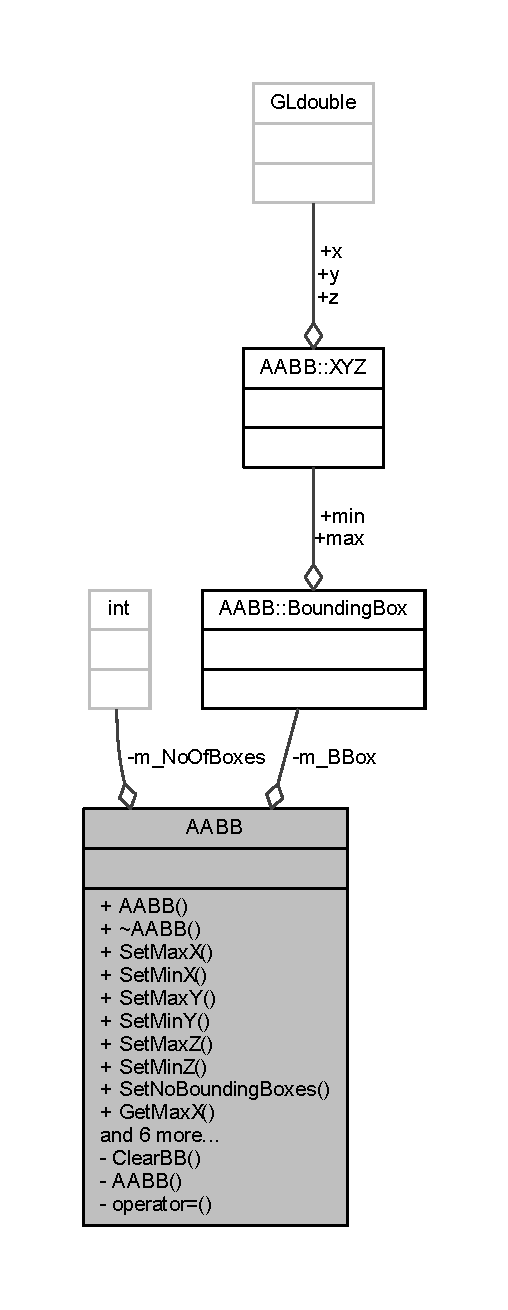
\includegraphics[height=550pt]{class_a_a_b_b__coll__graph}
\end{center}
\end{figure}
\subsection*{Classes}
\begin{DoxyCompactItemize}
\item 
struct \hyperlink{struct_a_a_b_b_1_1_bounding_box}{Bounding\+Box}
\item 
struct \hyperlink{struct_a_a_b_b_1_1_x_y_z}{X\+YZ}
\end{DoxyCompactItemize}
\subsection*{Public Member Functions}
\begin{DoxyCompactItemize}
\item 
\hyperlink{class_a_a_b_b_a5f5baf6c533905aa1456b3a3eb57bab2}{A\+A\+BB} ()
\item 
virtual \hyperlink{class_a_a_b_b_a1c8a263cbd356446535e88b521eab3d5}{$\sim$\+A\+A\+BB} ()
\item 
void \hyperlink{class_a_a_b_b_a49aefcac8e9b33ef4508f220d551e9a3}{Set\+MaxX} (const int \&temp\+Index, const G\+Ldouble \&tempX)
\item 
void \hyperlink{class_a_a_b_b_a38ecdedc213500ce61a1caa9ad0b1468}{Set\+MinX} (const int \&temp\+Index, const G\+Ldouble \&tempX)
\item 
void \hyperlink{class_a_a_b_b_af5f3fe38dd9aaf9ba1aa81c119b4beaa}{Set\+MaxY} (const int \&temp\+Index, const G\+Ldouble \&tempY)
\item 
void \hyperlink{class_a_a_b_b_a1cba0f0ef073d176fcffd58344668c6a}{Set\+MinY} (const int \&temp\+Index, const G\+Ldouble \&tempY)
\item 
void \hyperlink{class_a_a_b_b_a3b5c15b7a3330384d08b4ad1a8c87903}{Set\+MaxZ} (const int \&temp\+Index, const G\+Ldouble \&tempZ)
\item 
void \hyperlink{class_a_a_b_b_a97f330cb047e00b160cee87301b8ac23}{Set\+MinZ} (const int \&temp\+Index, const G\+Ldouble \&tempZ)
\item 
void \hyperlink{class_a_a_b_b_a4bbff0661c754b621c4b6bfc89bcf051}{Set\+No\+Bounding\+Boxes} (const int \&temp\+Size)
\item 
G\+Ldouble \hyperlink{class_a_a_b_b_a96d56ed1be5ba2a151b82c508d9149a2}{Get\+MaxX} (const int \&temp\+Index)
\item 
G\+Ldouble \hyperlink{class_a_a_b_b_a54aa8d1616469816102925c93cd7c195}{Get\+MinX} (const int \&temp\+Index)
\item 
G\+Ldouble \hyperlink{class_a_a_b_b_a1e4dc54e528b14528968b6aa9e347eea}{Get\+MaxY} (const int \&temp\+Index)
\item 
G\+Ldouble \hyperlink{class_a_a_b_b_a1177a0ebf40f7f3545f834f99c73c0f6}{Get\+MinY} (const int \&temp\+Index)
\item 
G\+Ldouble \hyperlink{class_a_a_b_b_a8f39211bf0b803194058797bcb06450c}{Get\+MaxZ} (const int \&temp\+Index)
\item 
G\+Ldouble \hyperlink{class_a_a_b_b_aaa4d9cd90b1f8890b9c678a2d33fb693}{Get\+MinZ} (const int \&temp\+Index)
\item 
int \hyperlink{class_a_a_b_b_a65be20483d52ea207e9569244c5fb1c4}{Get\+No\+Bounding\+Boxes} ()
\end{DoxyCompactItemize}
\subsection*{Private Member Functions}
\begin{DoxyCompactItemize}
\item 
void \hyperlink{class_a_a_b_b_a0c8c0d63af1044663eb095c43b53e1a6}{Clear\+BB} (\hyperlink{struct_a_a_b_b_1_1_bounding_box}{Bounding\+Box} $\ast$\&temp\+Array)
\item 
\hyperlink{class_a_a_b_b_a7a43651ebd0edfde0fe707afc97295fa}{A\+A\+BB} (const \hyperlink{class_a_a_b_b}{A\+A\+BB} \&aabb)
\item 
\hyperlink{class_a_a_b_b}{A\+A\+BB} \& \hyperlink{class_a_a_b_b_a5e03a183f9968778603af55af5dbfea4}{operator=} (const \hyperlink{class_a_a_b_b}{A\+A\+BB} \&aabb)
\end{DoxyCompactItemize}
\subsection*{Private Attributes}
\begin{DoxyCompactItemize}
\item 
\hyperlink{struct_a_a_b_b_1_1_bounding_box}{Bounding\+Box} $\ast$ \hyperlink{class_a_a_b_b_a0085dacc83197350a4d4f114ff67ddd4}{m\+\_\+\+B\+Box}
\item 
int \hyperlink{class_a_a_b_b_a7b66c322f9e990757be44203e7b5d76a}{m\+\_\+\+No\+Of\+Boxes}
\end{DoxyCompactItemize}


\subsection{Constructor \& Destructor Documentation}
\index{A\+A\+BB@{A\+A\+BB}!A\+A\+BB@{A\+A\+BB}}
\index{A\+A\+BB@{A\+A\+BB}!A\+A\+BB@{A\+A\+BB}}
\subsubsection[{\texorpdfstring{A\+A\+B\+B(const A\+A\+B\+B \&aabb)}{AABB(const AABB &aabb)}}]{\setlength{\rightskip}{0pt plus 5cm}A\+A\+B\+B\+::\+A\+A\+BB (
\begin{DoxyParamCaption}
\item[{const {\bf A\+A\+BB} \&}]{aabb}
\end{DoxyParamCaption}
)\hspace{0.3cm}{\ttfamily [inline]}, {\ttfamily [private]}}\hypertarget{class_a_a_b_b_a7a43651ebd0edfde0fe707afc97295fa}{}\label{class_a_a_b_b_a7a43651ebd0edfde0fe707afc97295fa}
\index{A\+A\+BB@{A\+A\+BB}!A\+A\+BB@{A\+A\+BB}}
\index{A\+A\+BB@{A\+A\+BB}!A\+A\+BB@{A\+A\+BB}}
\subsubsection[{\texorpdfstring{A\+A\+B\+B()}{AABB()}}]{\setlength{\rightskip}{0pt plus 5cm}A\+A\+B\+B\+::\+A\+A\+BB (
\begin{DoxyParamCaption}
{}
\end{DoxyParamCaption}
)\hspace{0.3cm}{\ttfamily [inline]}}\hypertarget{class_a_a_b_b_a5f5baf6c533905aa1456b3a3eb57bab2}{}\label{class_a_a_b_b_a5f5baf6c533905aa1456b3a3eb57bab2}
\index{A\+A\+BB@{A\+A\+BB}!````~A\+A\+BB@{$\sim$\+A\+A\+BB}}
\index{````~A\+A\+BB@{$\sim$\+A\+A\+BB}!A\+A\+BB@{A\+A\+BB}}
\subsubsection[{\texorpdfstring{$\sim$\+A\+A\+B\+B()}{~AABB()}}]{\setlength{\rightskip}{0pt plus 5cm}virtual A\+A\+B\+B\+::$\sim$\+A\+A\+BB (
\begin{DoxyParamCaption}
{}
\end{DoxyParamCaption}
)\hspace{0.3cm}{\ttfamily [inline]}, {\ttfamily [virtual]}}\hypertarget{class_a_a_b_b_a1c8a263cbd356446535e88b521eab3d5}{}\label{class_a_a_b_b_a1c8a263cbd356446535e88b521eab3d5}


Here is the call graph for this function\+:
\nopagebreak
\begin{figure}[H]
\begin{center}
\leavevmode
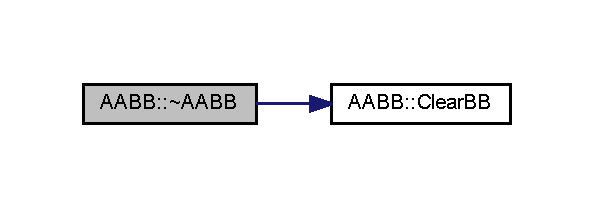
\includegraphics[width=285pt]{class_a_a_b_b_a1c8a263cbd356446535e88b521eab3d5_cgraph}
\end{center}
\end{figure}




Here is the caller graph for this function\+:
\nopagebreak
\begin{figure}[H]
\begin{center}
\leavevmode
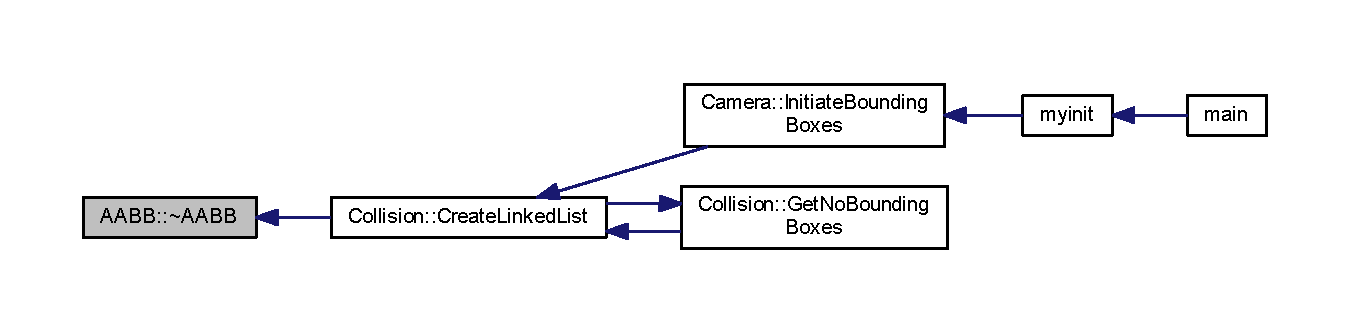
\includegraphics[width=350pt]{class_a_a_b_b_a1c8a263cbd356446535e88b521eab3d5_icgraph}
\end{center}
\end{figure}




\subsection{Member Function Documentation}
\index{A\+A\+BB@{A\+A\+BB}!Clear\+BB@{Clear\+BB}}
\index{Clear\+BB@{Clear\+BB}!A\+A\+BB@{A\+A\+BB}}
\subsubsection[{\texorpdfstring{Clear\+B\+B(\+Bounding\+Box $\ast$\&temp\+Array)}{ClearBB(BoundingBox *&tempArray)}}]{\setlength{\rightskip}{0pt plus 5cm}void A\+A\+B\+B\+::\+Clear\+BB (
\begin{DoxyParamCaption}
\item[{{\bf Bounding\+Box} $\ast$\&}]{temp\+Array}
\end{DoxyParamCaption}
)\hspace{0.3cm}{\ttfamily [private]}}\hypertarget{class_a_a_b_b_a0c8c0d63af1044663eb095c43b53e1a6}{}\label{class_a_a_b_b_a0c8c0d63af1044663eb095c43b53e1a6}


Here is the caller graph for this function\+:
\nopagebreak
\begin{figure}[H]
\begin{center}
\leavevmode
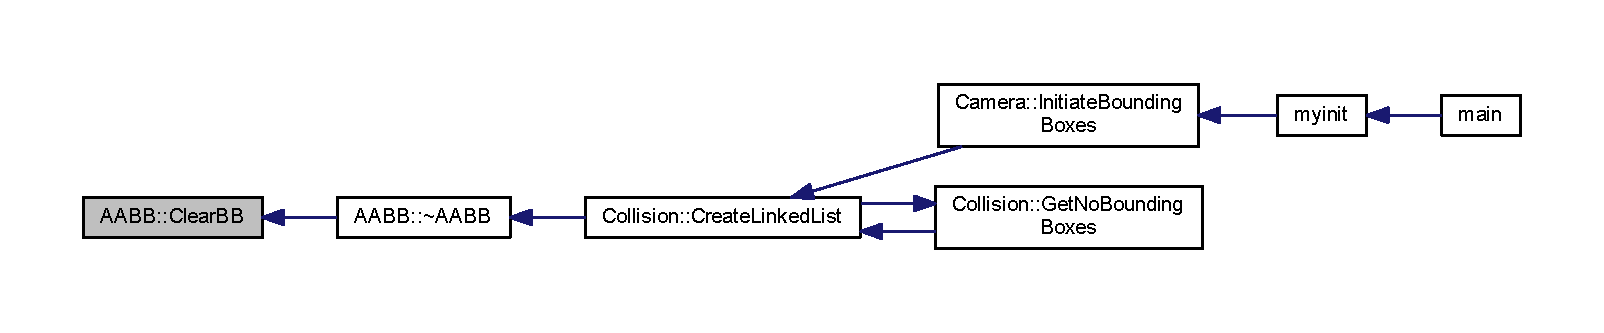
\includegraphics[width=350pt]{class_a_a_b_b_a0c8c0d63af1044663eb095c43b53e1a6_icgraph}
\end{center}
\end{figure}


\index{A\+A\+BB@{A\+A\+BB}!Get\+MaxX@{Get\+MaxX}}
\index{Get\+MaxX@{Get\+MaxX}!A\+A\+BB@{A\+A\+BB}}
\subsubsection[{\texorpdfstring{Get\+Max\+X(const int \&temp\+Index)}{GetMaxX(const int &tempIndex)}}]{\setlength{\rightskip}{0pt plus 5cm}G\+Ldouble A\+A\+B\+B\+::\+Get\+MaxX (
\begin{DoxyParamCaption}
\item[{const int \&}]{temp\+Index}
\end{DoxyParamCaption}
)\hspace{0.3cm}{\ttfamily [inline]}}\hypertarget{class_a_a_b_b_a96d56ed1be5ba2a151b82c508d9149a2}{}\label{class_a_a_b_b_a96d56ed1be5ba2a151b82c508d9149a2}


Here is the caller graph for this function\+:
\nopagebreak
\begin{figure}[H]
\begin{center}
\leavevmode
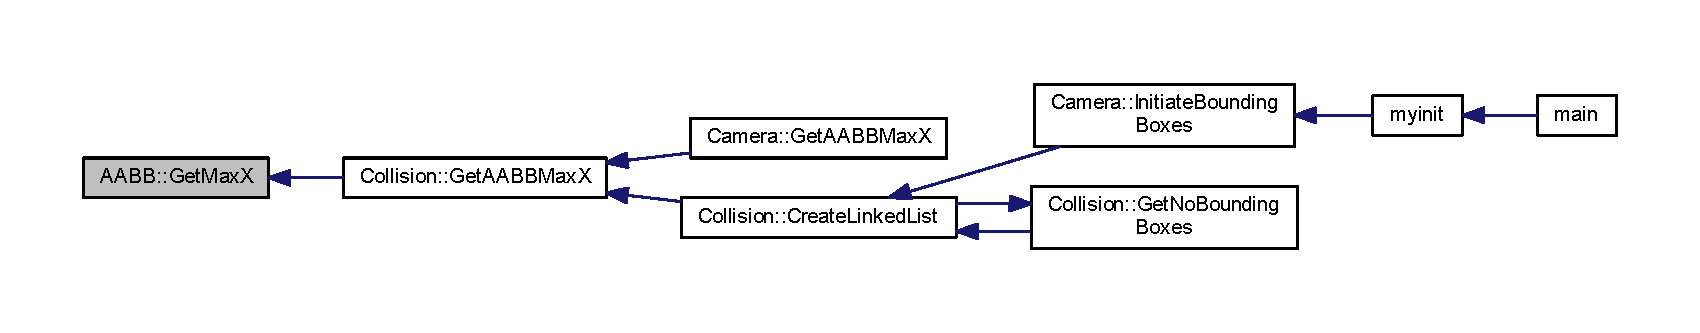
\includegraphics[width=350pt]{class_a_a_b_b_a96d56ed1be5ba2a151b82c508d9149a2_icgraph}
\end{center}
\end{figure}


\index{A\+A\+BB@{A\+A\+BB}!Get\+MaxY@{Get\+MaxY}}
\index{Get\+MaxY@{Get\+MaxY}!A\+A\+BB@{A\+A\+BB}}
\subsubsection[{\texorpdfstring{Get\+Max\+Y(const int \&temp\+Index)}{GetMaxY(const int &tempIndex)}}]{\setlength{\rightskip}{0pt plus 5cm}G\+Ldouble A\+A\+B\+B\+::\+Get\+MaxY (
\begin{DoxyParamCaption}
\item[{const int \&}]{temp\+Index}
\end{DoxyParamCaption}
)\hspace{0.3cm}{\ttfamily [inline]}}\hypertarget{class_a_a_b_b_a1e4dc54e528b14528968b6aa9e347eea}{}\label{class_a_a_b_b_a1e4dc54e528b14528968b6aa9e347eea}


Here is the caller graph for this function\+:
\nopagebreak
\begin{figure}[H]
\begin{center}
\leavevmode
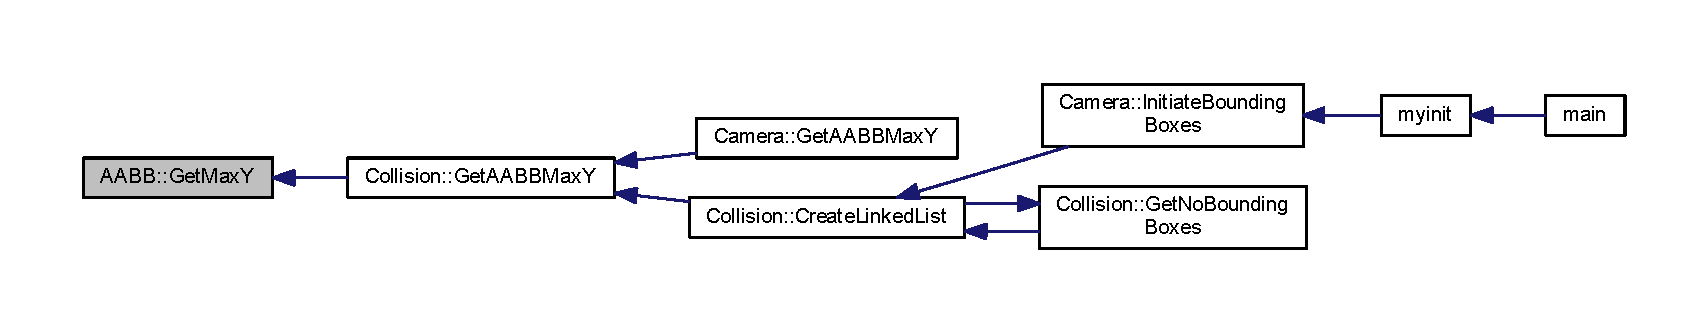
\includegraphics[width=350pt]{class_a_a_b_b_a1e4dc54e528b14528968b6aa9e347eea_icgraph}
\end{center}
\end{figure}


\index{A\+A\+BB@{A\+A\+BB}!Get\+MaxZ@{Get\+MaxZ}}
\index{Get\+MaxZ@{Get\+MaxZ}!A\+A\+BB@{A\+A\+BB}}
\subsubsection[{\texorpdfstring{Get\+Max\+Z(const int \&temp\+Index)}{GetMaxZ(const int &tempIndex)}}]{\setlength{\rightskip}{0pt plus 5cm}G\+Ldouble A\+A\+B\+B\+::\+Get\+MaxZ (
\begin{DoxyParamCaption}
\item[{const int \&}]{temp\+Index}
\end{DoxyParamCaption}
)\hspace{0.3cm}{\ttfamily [inline]}}\hypertarget{class_a_a_b_b_a8f39211bf0b803194058797bcb06450c}{}\label{class_a_a_b_b_a8f39211bf0b803194058797bcb06450c}


Here is the caller graph for this function\+:
\nopagebreak
\begin{figure}[H]
\begin{center}
\leavevmode
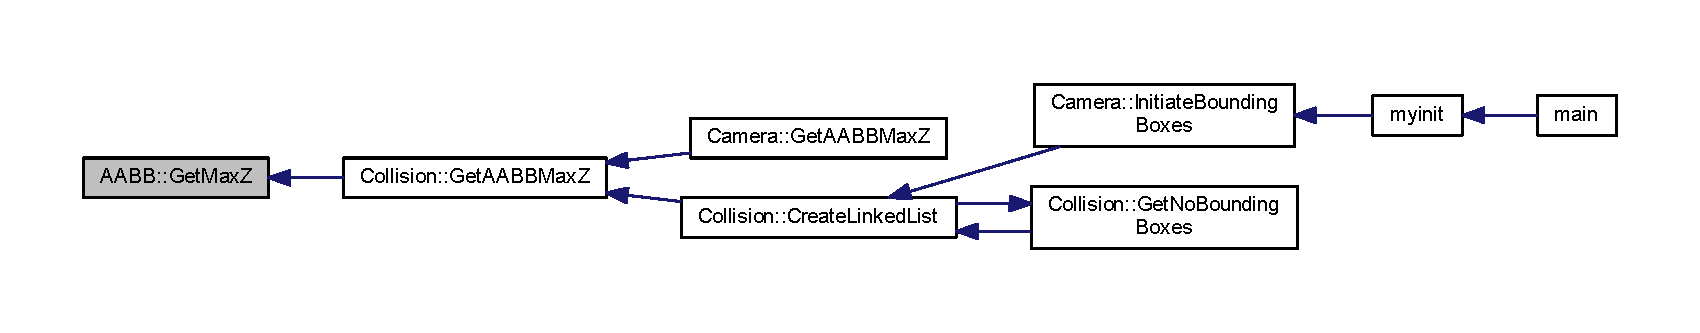
\includegraphics[width=350pt]{class_a_a_b_b_a8f39211bf0b803194058797bcb06450c_icgraph}
\end{center}
\end{figure}


\index{A\+A\+BB@{A\+A\+BB}!Get\+MinX@{Get\+MinX}}
\index{Get\+MinX@{Get\+MinX}!A\+A\+BB@{A\+A\+BB}}
\subsubsection[{\texorpdfstring{Get\+Min\+X(const int \&temp\+Index)}{GetMinX(const int &tempIndex)}}]{\setlength{\rightskip}{0pt plus 5cm}G\+Ldouble A\+A\+B\+B\+::\+Get\+MinX (
\begin{DoxyParamCaption}
\item[{const int \&}]{temp\+Index}
\end{DoxyParamCaption}
)\hspace{0.3cm}{\ttfamily [inline]}}\hypertarget{class_a_a_b_b_a54aa8d1616469816102925c93cd7c195}{}\label{class_a_a_b_b_a54aa8d1616469816102925c93cd7c195}


Here is the caller graph for this function\+:
\nopagebreak
\begin{figure}[H]
\begin{center}
\leavevmode
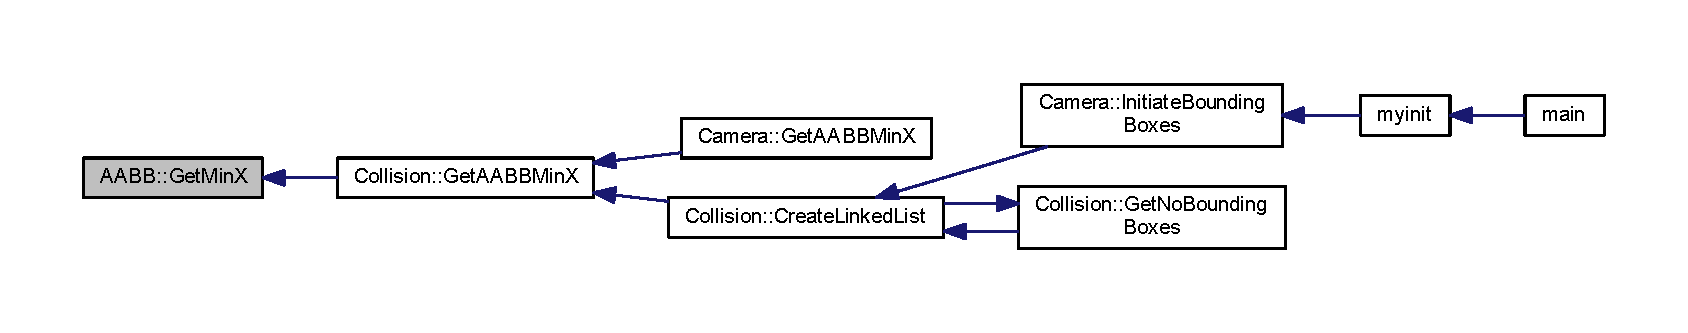
\includegraphics[width=350pt]{class_a_a_b_b_a54aa8d1616469816102925c93cd7c195_icgraph}
\end{center}
\end{figure}


\index{A\+A\+BB@{A\+A\+BB}!Get\+MinY@{Get\+MinY}}
\index{Get\+MinY@{Get\+MinY}!A\+A\+BB@{A\+A\+BB}}
\subsubsection[{\texorpdfstring{Get\+Min\+Y(const int \&temp\+Index)}{GetMinY(const int &tempIndex)}}]{\setlength{\rightskip}{0pt plus 5cm}G\+Ldouble A\+A\+B\+B\+::\+Get\+MinY (
\begin{DoxyParamCaption}
\item[{const int \&}]{temp\+Index}
\end{DoxyParamCaption}
)\hspace{0.3cm}{\ttfamily [inline]}}\hypertarget{class_a_a_b_b_a1177a0ebf40f7f3545f834f99c73c0f6}{}\label{class_a_a_b_b_a1177a0ebf40f7f3545f834f99c73c0f6}


Here is the caller graph for this function\+:
\nopagebreak
\begin{figure}[H]
\begin{center}
\leavevmode
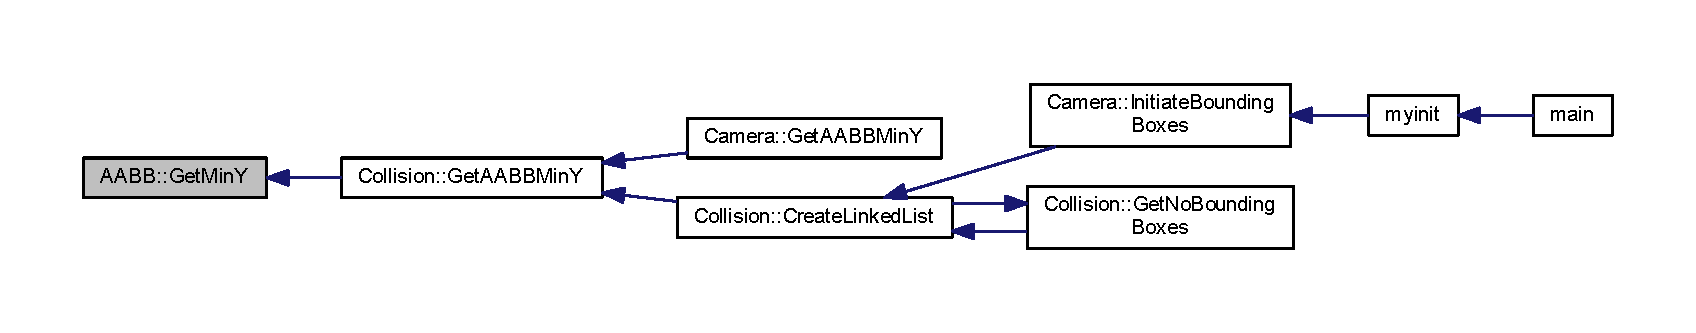
\includegraphics[width=350pt]{class_a_a_b_b_a1177a0ebf40f7f3545f834f99c73c0f6_icgraph}
\end{center}
\end{figure}


\index{A\+A\+BB@{A\+A\+BB}!Get\+MinZ@{Get\+MinZ}}
\index{Get\+MinZ@{Get\+MinZ}!A\+A\+BB@{A\+A\+BB}}
\subsubsection[{\texorpdfstring{Get\+Min\+Z(const int \&temp\+Index)}{GetMinZ(const int &tempIndex)}}]{\setlength{\rightskip}{0pt plus 5cm}G\+Ldouble A\+A\+B\+B\+::\+Get\+MinZ (
\begin{DoxyParamCaption}
\item[{const int \&}]{temp\+Index}
\end{DoxyParamCaption}
)\hspace{0.3cm}{\ttfamily [inline]}}\hypertarget{class_a_a_b_b_aaa4d9cd90b1f8890b9c678a2d33fb693}{}\label{class_a_a_b_b_aaa4d9cd90b1f8890b9c678a2d33fb693}


Here is the caller graph for this function\+:
\nopagebreak
\begin{figure}[H]
\begin{center}
\leavevmode
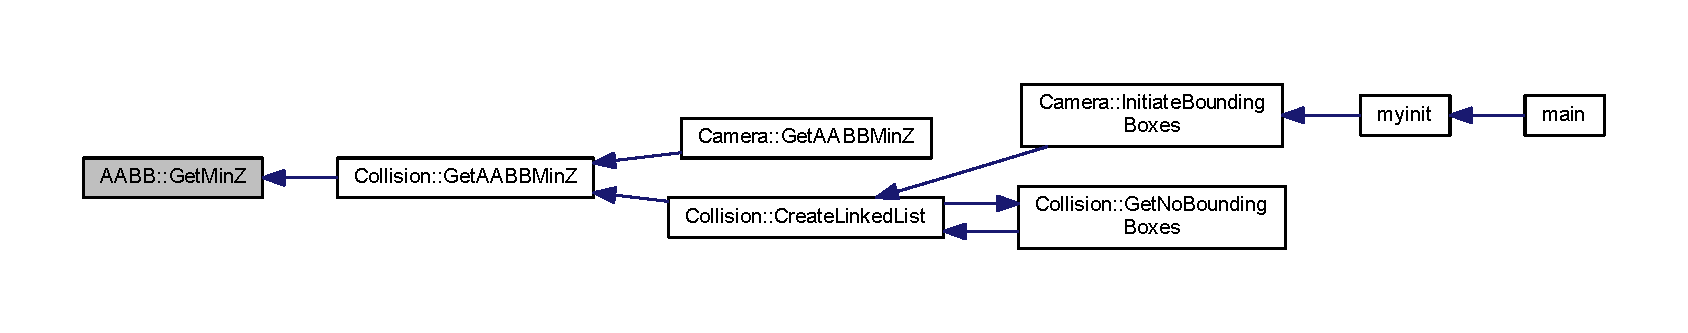
\includegraphics[width=350pt]{class_a_a_b_b_aaa4d9cd90b1f8890b9c678a2d33fb693_icgraph}
\end{center}
\end{figure}


\index{A\+A\+BB@{A\+A\+BB}!Get\+No\+Bounding\+Boxes@{Get\+No\+Bounding\+Boxes}}
\index{Get\+No\+Bounding\+Boxes@{Get\+No\+Bounding\+Boxes}!A\+A\+BB@{A\+A\+BB}}
\subsubsection[{\texorpdfstring{Get\+No\+Bounding\+Boxes()}{GetNoBoundingBoxes()}}]{\setlength{\rightskip}{0pt plus 5cm}int A\+A\+B\+B\+::\+Get\+No\+Bounding\+Boxes (
\begin{DoxyParamCaption}
{}
\end{DoxyParamCaption}
)\hspace{0.3cm}{\ttfamily [inline]}}\hypertarget{class_a_a_b_b_a65be20483d52ea207e9569244c5fb1c4}{}\label{class_a_a_b_b_a65be20483d52ea207e9569244c5fb1c4}


Here is the caller graph for this function\+:
\nopagebreak
\begin{figure}[H]
\begin{center}
\leavevmode
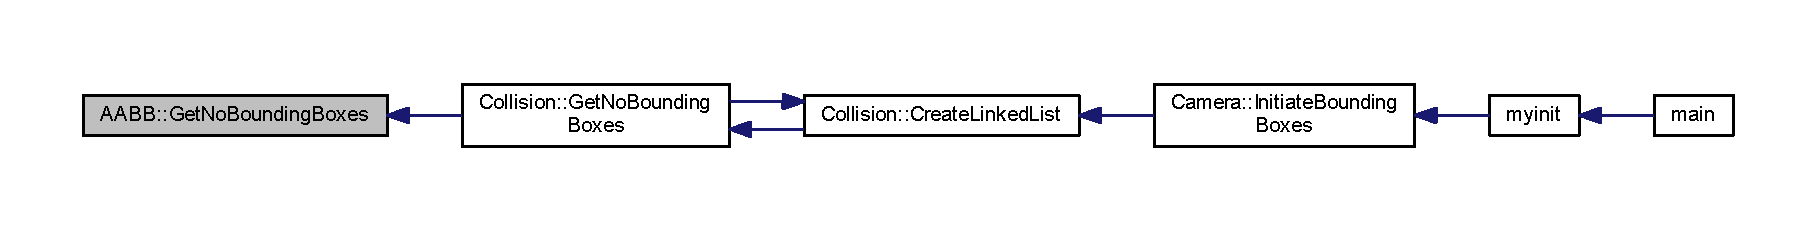
\includegraphics[width=350pt]{class_a_a_b_b_a65be20483d52ea207e9569244c5fb1c4_icgraph}
\end{center}
\end{figure}


\index{A\+A\+BB@{A\+A\+BB}!operator=@{operator=}}
\index{operator=@{operator=}!A\+A\+BB@{A\+A\+BB}}
\subsubsection[{\texorpdfstring{operator=(const A\+A\+B\+B \&aabb)}{operator=(const AABB &aabb)}}]{\setlength{\rightskip}{0pt plus 5cm}{\bf A\+A\+BB}\& A\+A\+B\+B\+::operator= (
\begin{DoxyParamCaption}
\item[{const {\bf A\+A\+BB} \&}]{aabb}
\end{DoxyParamCaption}
)\hspace{0.3cm}{\ttfamily [inline]}, {\ttfamily [private]}}\hypertarget{class_a_a_b_b_a5e03a183f9968778603af55af5dbfea4}{}\label{class_a_a_b_b_a5e03a183f9968778603af55af5dbfea4}
\index{A\+A\+BB@{A\+A\+BB}!Set\+MaxX@{Set\+MaxX}}
\index{Set\+MaxX@{Set\+MaxX}!A\+A\+BB@{A\+A\+BB}}
\subsubsection[{\texorpdfstring{Set\+Max\+X(const int \&temp\+Index, const G\+Ldouble \&temp\+X)}{SetMaxX(const int &tempIndex, const GLdouble &tempX)}}]{\setlength{\rightskip}{0pt plus 5cm}void A\+A\+B\+B\+::\+Set\+MaxX (
\begin{DoxyParamCaption}
\item[{const int \&}]{temp\+Index, }
\item[{const G\+Ldouble \&}]{tempX}
\end{DoxyParamCaption}
)\hspace{0.3cm}{\ttfamily [inline]}}\hypertarget{class_a_a_b_b_a49aefcac8e9b33ef4508f220d551e9a3}{}\label{class_a_a_b_b_a49aefcac8e9b33ef4508f220d551e9a3}


Here is the caller graph for this function\+:
\nopagebreak
\begin{figure}[H]
\begin{center}
\leavevmode
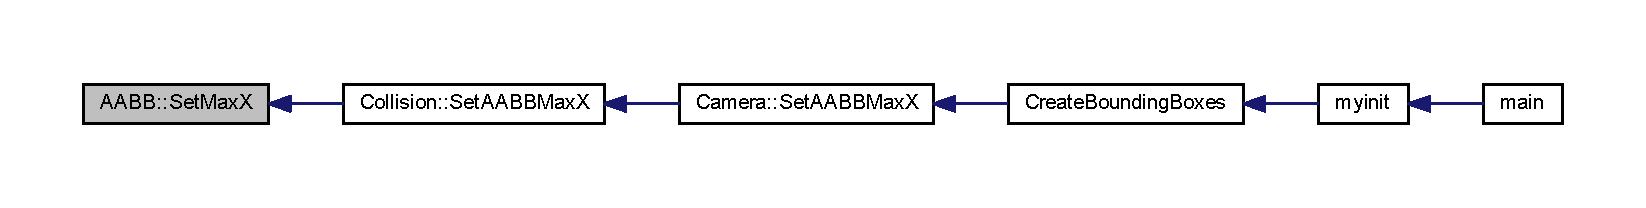
\includegraphics[width=350pt]{class_a_a_b_b_a49aefcac8e9b33ef4508f220d551e9a3_icgraph}
\end{center}
\end{figure}


\index{A\+A\+BB@{A\+A\+BB}!Set\+MaxY@{Set\+MaxY}}
\index{Set\+MaxY@{Set\+MaxY}!A\+A\+BB@{A\+A\+BB}}
\subsubsection[{\texorpdfstring{Set\+Max\+Y(const int \&temp\+Index, const G\+Ldouble \&temp\+Y)}{SetMaxY(const int &tempIndex, const GLdouble &tempY)}}]{\setlength{\rightskip}{0pt plus 5cm}void A\+A\+B\+B\+::\+Set\+MaxY (
\begin{DoxyParamCaption}
\item[{const int \&}]{temp\+Index, }
\item[{const G\+Ldouble \&}]{tempY}
\end{DoxyParamCaption}
)\hspace{0.3cm}{\ttfamily [inline]}}\hypertarget{class_a_a_b_b_af5f3fe38dd9aaf9ba1aa81c119b4beaa}{}\label{class_a_a_b_b_af5f3fe38dd9aaf9ba1aa81c119b4beaa}


Here is the caller graph for this function\+:
\nopagebreak
\begin{figure}[H]
\begin{center}
\leavevmode
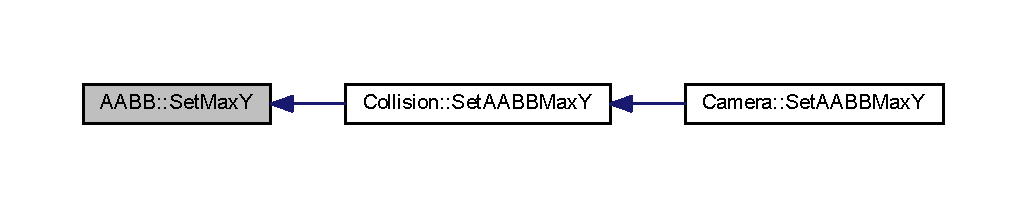
\includegraphics[width=350pt]{class_a_a_b_b_af5f3fe38dd9aaf9ba1aa81c119b4beaa_icgraph}
\end{center}
\end{figure}


\index{A\+A\+BB@{A\+A\+BB}!Set\+MaxZ@{Set\+MaxZ}}
\index{Set\+MaxZ@{Set\+MaxZ}!A\+A\+BB@{A\+A\+BB}}
\subsubsection[{\texorpdfstring{Set\+Max\+Z(const int \&temp\+Index, const G\+Ldouble \&temp\+Z)}{SetMaxZ(const int &tempIndex, const GLdouble &tempZ)}}]{\setlength{\rightskip}{0pt plus 5cm}void A\+A\+B\+B\+::\+Set\+MaxZ (
\begin{DoxyParamCaption}
\item[{const int \&}]{temp\+Index, }
\item[{const G\+Ldouble \&}]{tempZ}
\end{DoxyParamCaption}
)\hspace{0.3cm}{\ttfamily [inline]}}\hypertarget{class_a_a_b_b_a3b5c15b7a3330384d08b4ad1a8c87903}{}\label{class_a_a_b_b_a3b5c15b7a3330384d08b4ad1a8c87903}


Here is the caller graph for this function\+:
\nopagebreak
\begin{figure}[H]
\begin{center}
\leavevmode
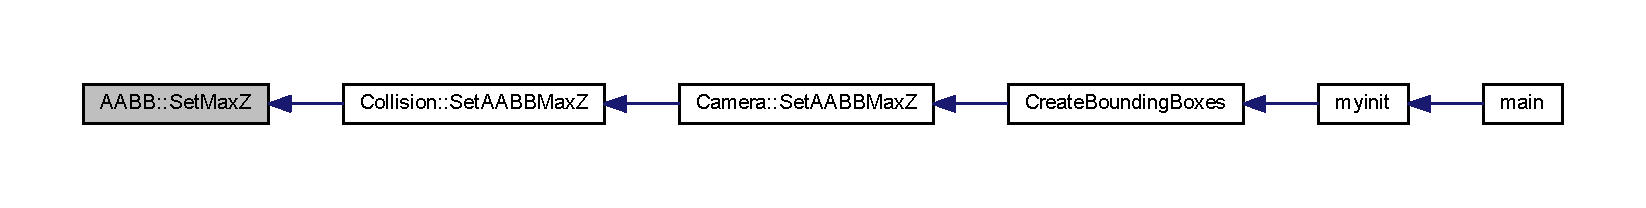
\includegraphics[width=350pt]{class_a_a_b_b_a3b5c15b7a3330384d08b4ad1a8c87903_icgraph}
\end{center}
\end{figure}


\index{A\+A\+BB@{A\+A\+BB}!Set\+MinX@{Set\+MinX}}
\index{Set\+MinX@{Set\+MinX}!A\+A\+BB@{A\+A\+BB}}
\subsubsection[{\texorpdfstring{Set\+Min\+X(const int \&temp\+Index, const G\+Ldouble \&temp\+X)}{SetMinX(const int &tempIndex, const GLdouble &tempX)}}]{\setlength{\rightskip}{0pt plus 5cm}void A\+A\+B\+B\+::\+Set\+MinX (
\begin{DoxyParamCaption}
\item[{const int \&}]{temp\+Index, }
\item[{const G\+Ldouble \&}]{tempX}
\end{DoxyParamCaption}
)\hspace{0.3cm}{\ttfamily [inline]}}\hypertarget{class_a_a_b_b_a38ecdedc213500ce61a1caa9ad0b1468}{}\label{class_a_a_b_b_a38ecdedc213500ce61a1caa9ad0b1468}


Here is the caller graph for this function\+:
\nopagebreak
\begin{figure}[H]
\begin{center}
\leavevmode
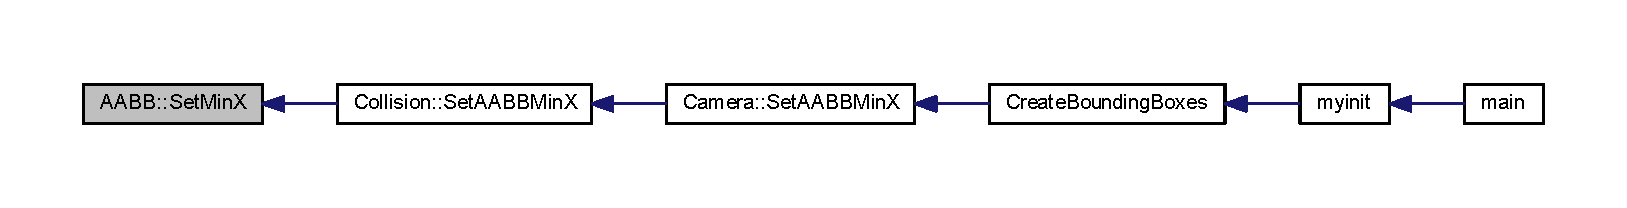
\includegraphics[width=350pt]{class_a_a_b_b_a38ecdedc213500ce61a1caa9ad0b1468_icgraph}
\end{center}
\end{figure}


\index{A\+A\+BB@{A\+A\+BB}!Set\+MinY@{Set\+MinY}}
\index{Set\+MinY@{Set\+MinY}!A\+A\+BB@{A\+A\+BB}}
\subsubsection[{\texorpdfstring{Set\+Min\+Y(const int \&temp\+Index, const G\+Ldouble \&temp\+Y)}{SetMinY(const int &tempIndex, const GLdouble &tempY)}}]{\setlength{\rightskip}{0pt plus 5cm}void A\+A\+B\+B\+::\+Set\+MinY (
\begin{DoxyParamCaption}
\item[{const int \&}]{temp\+Index, }
\item[{const G\+Ldouble \&}]{tempY}
\end{DoxyParamCaption}
)\hspace{0.3cm}{\ttfamily [inline]}}\hypertarget{class_a_a_b_b_a1cba0f0ef073d176fcffd58344668c6a}{}\label{class_a_a_b_b_a1cba0f0ef073d176fcffd58344668c6a}


Here is the caller graph for this function\+:
\nopagebreak
\begin{figure}[H]
\begin{center}
\leavevmode
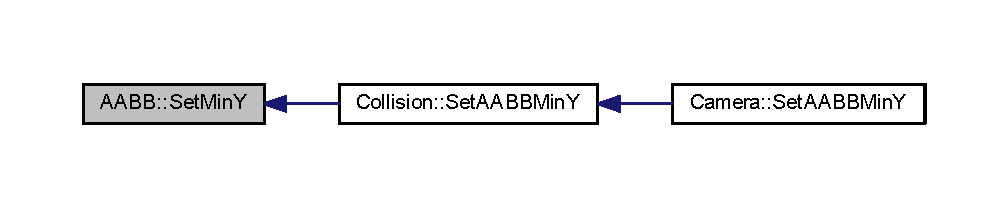
\includegraphics[width=350pt]{class_a_a_b_b_a1cba0f0ef073d176fcffd58344668c6a_icgraph}
\end{center}
\end{figure}


\index{A\+A\+BB@{A\+A\+BB}!Set\+MinZ@{Set\+MinZ}}
\index{Set\+MinZ@{Set\+MinZ}!A\+A\+BB@{A\+A\+BB}}
\subsubsection[{\texorpdfstring{Set\+Min\+Z(const int \&temp\+Index, const G\+Ldouble \&temp\+Z)}{SetMinZ(const int &tempIndex, const GLdouble &tempZ)}}]{\setlength{\rightskip}{0pt plus 5cm}void A\+A\+B\+B\+::\+Set\+MinZ (
\begin{DoxyParamCaption}
\item[{const int \&}]{temp\+Index, }
\item[{const G\+Ldouble \&}]{tempZ}
\end{DoxyParamCaption}
)\hspace{0.3cm}{\ttfamily [inline]}}\hypertarget{class_a_a_b_b_a97f330cb047e00b160cee87301b8ac23}{}\label{class_a_a_b_b_a97f330cb047e00b160cee87301b8ac23}


Here is the call graph for this function\+:
\nopagebreak
\begin{figure}[H]
\begin{center}
\leavevmode
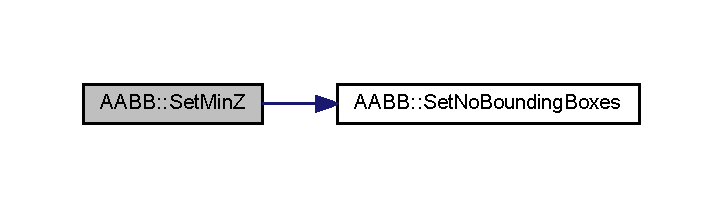
\includegraphics[width=347pt]{class_a_a_b_b_a97f330cb047e00b160cee87301b8ac23_cgraph}
\end{center}
\end{figure}




Here is the caller graph for this function\+:
\nopagebreak
\begin{figure}[H]
\begin{center}
\leavevmode
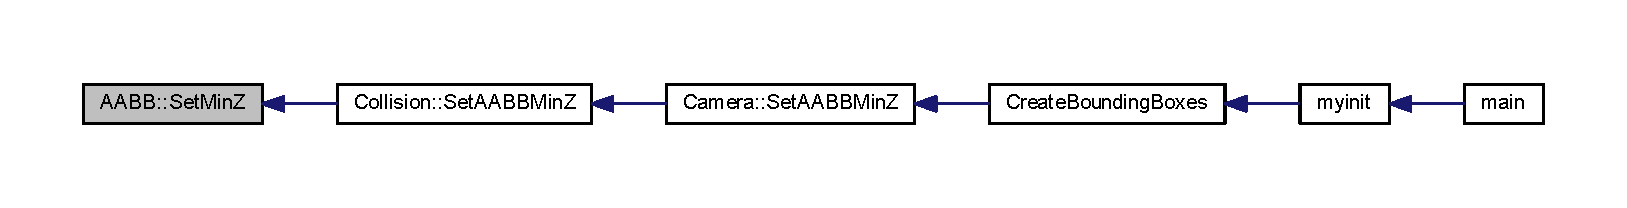
\includegraphics[width=350pt]{class_a_a_b_b_a97f330cb047e00b160cee87301b8ac23_icgraph}
\end{center}
\end{figure}


\index{A\+A\+BB@{A\+A\+BB}!Set\+No\+Bounding\+Boxes@{Set\+No\+Bounding\+Boxes}}
\index{Set\+No\+Bounding\+Boxes@{Set\+No\+Bounding\+Boxes}!A\+A\+BB@{A\+A\+BB}}
\subsubsection[{\texorpdfstring{Set\+No\+Bounding\+Boxes(const int \&temp\+Size)}{SetNoBoundingBoxes(const int &tempSize)}}]{\setlength{\rightskip}{0pt plus 5cm}void A\+A\+B\+B\+::\+Set\+No\+Bounding\+Boxes (
\begin{DoxyParamCaption}
\item[{const int \&}]{temp\+Size}
\end{DoxyParamCaption}
)}\hypertarget{class_a_a_b_b_a4bbff0661c754b621c4b6bfc89bcf051}{}\label{class_a_a_b_b_a4bbff0661c754b621c4b6bfc89bcf051}


Here is the caller graph for this function\+:
\nopagebreak
\begin{figure}[H]
\begin{center}
\leavevmode
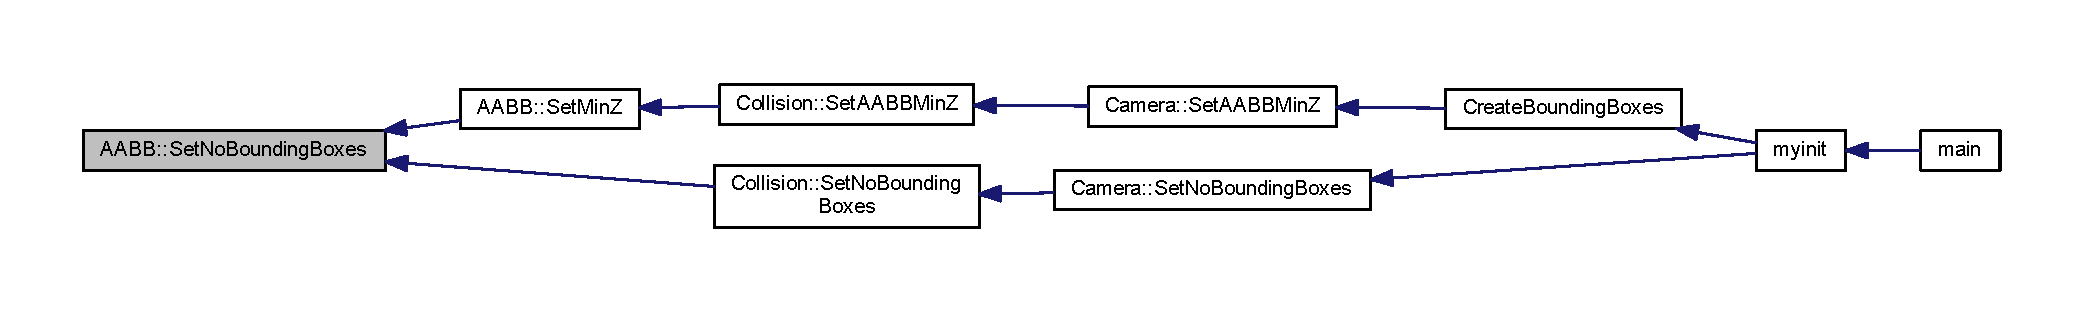
\includegraphics[width=350pt]{class_a_a_b_b_a4bbff0661c754b621c4b6bfc89bcf051_icgraph}
\end{center}
\end{figure}




\subsection{Member Data Documentation}
\index{A\+A\+BB@{A\+A\+BB}!m\+\_\+\+B\+Box@{m\+\_\+\+B\+Box}}
\index{m\+\_\+\+B\+Box@{m\+\_\+\+B\+Box}!A\+A\+BB@{A\+A\+BB}}
\subsubsection[{\texorpdfstring{m\+\_\+\+B\+Box}{m_BBox}}]{\setlength{\rightskip}{0pt plus 5cm}{\bf Bounding\+Box}$\ast$ A\+A\+B\+B\+::m\+\_\+\+B\+Box\hspace{0.3cm}{\ttfamily [private]}}\hypertarget{class_a_a_b_b_a0085dacc83197350a4d4f114ff67ddd4}{}\label{class_a_a_b_b_a0085dacc83197350a4d4f114ff67ddd4}
\index{A\+A\+BB@{A\+A\+BB}!m\+\_\+\+No\+Of\+Boxes@{m\+\_\+\+No\+Of\+Boxes}}
\index{m\+\_\+\+No\+Of\+Boxes@{m\+\_\+\+No\+Of\+Boxes}!A\+A\+BB@{A\+A\+BB}}
\subsubsection[{\texorpdfstring{m\+\_\+\+No\+Of\+Boxes}{m_NoOfBoxes}}]{\setlength{\rightskip}{0pt plus 5cm}int A\+A\+B\+B\+::m\+\_\+\+No\+Of\+Boxes\hspace{0.3cm}{\ttfamily [private]}}\hypertarget{class_a_a_b_b_a7b66c322f9e990757be44203e7b5d76a}{}\label{class_a_a_b_b_a7b66c322f9e990757be44203e7b5d76a}


The documentation for this class was generated from the following files\+:\begin{DoxyCompactItemize}
\item 
C\+:/000\+Uniwork/\+I\+C\+T290 Games Programming Try 2/\+Exercise 1/\+C\+A\+M\+P\+U\+S T\+O\+U\+R/\hyperlink{_a_a_b_b_8_h}{A\+A\+B\+B.\+H}\item 
C\+:/000\+Uniwork/\+I\+C\+T290 Games Programming Try 2/\+Exercise 1/\+C\+A\+M\+P\+U\+S T\+O\+U\+R/\hyperlink{_a_a_b_b_8_c_p_p}{A\+A\+B\+B.\+C\+PP}\end{DoxyCompactItemize}

\hypertarget{class_a_a_b_b_linked_list}{}\section{A\+A\+B\+B\+Linked\+List Class Reference}
\label{class_a_a_b_b_linked_list}\index{A\+A\+B\+B\+Linked\+List@{A\+A\+B\+B\+Linked\+List}}


{\ttfamily \#include $<$A\+A\+B\+B\+Linked\+List.\+h$>$}



Collaboration diagram for A\+A\+B\+B\+Linked\+List\+:
\nopagebreak
\begin{figure}[H]
\begin{center}
\leavevmode
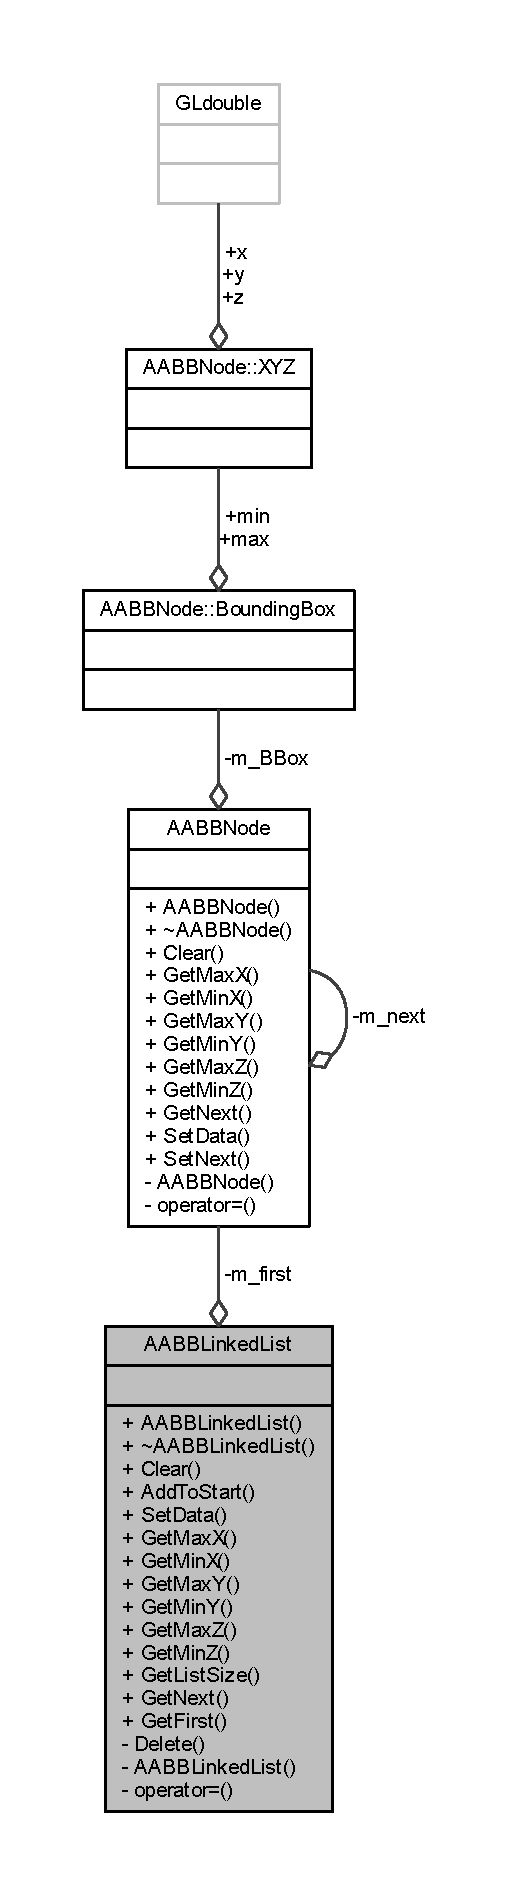
\includegraphics[height=550pt]{class_a_a_b_b_linked_list__coll__graph}
\end{center}
\end{figure}
\subsection*{Public Member Functions}
\begin{DoxyCompactItemize}
\item 
\hyperlink{class_a_a_b_b_linked_list_a2da1cd31c139b1ff1dd058f89c05c392}{A\+A\+B\+B\+Linked\+List} ()
\item 
virtual \hyperlink{class_a_a_b_b_linked_list_a045b677f4cceafb09d188e7a08f5e065}{$\sim$\+A\+A\+B\+B\+Linked\+List} ()
\item 
void \hyperlink{class_a_a_b_b_linked_list_a91220ba141deab9a3da2ec7ca6396436}{Clear} ()
\item 
bool \hyperlink{class_a_a_b_b_linked_list_a0dda8d1e7b9d5a2721b518d03b141664}{Add\+To\+Start} (G\+Ldouble maxX, G\+Ldouble minX, G\+Ldouble maxY, G\+Ldouble minY, G\+Ldouble maxZ, G\+Ldouble minZ)
\item 
void \hyperlink{class_a_a_b_b_linked_list_a9466a3aaffb597d9976259726b44463a}{Set\+Data} (const int \&ptr\+Count, const G\+Ldouble maxX, const G\+Ldouble minX, const G\+Ldouble maxY, const G\+Ldouble minY, const G\+Ldouble maxZ, const G\+Ldouble minZ)
\item 
G\+Ldouble \hyperlink{class_a_a_b_b_linked_list_a8e5dfc22a5b09a5439c7d48c777f21b6}{Get\+MaxX} (int ptr\+Count)
\item 
G\+Ldouble \hyperlink{class_a_a_b_b_linked_list_a01b738ef73d102240bc9bd54044c2a46}{Get\+MinX} (int ptr\+Count)
\item 
G\+Ldouble \hyperlink{class_a_a_b_b_linked_list_a06e37c604e86a670fc6657aac7ada31b}{Get\+MaxY} (int ptr\+Count)
\item 
G\+Ldouble \hyperlink{class_a_a_b_b_linked_list_aa59cbdbfb2012f733010283639a27584}{Get\+MinY} (int ptr\+Count)
\item 
G\+Ldouble \hyperlink{class_a_a_b_b_linked_list_af728cb9e63fe37667356ec4a74d9bb09}{Get\+MaxZ} (int ptr\+Count)
\item 
G\+Ldouble \hyperlink{class_a_a_b_b_linked_list_a93270a86be1d2f63aca450f7ef39d130}{Get\+MinZ} (int ptr\+Count)
\item 
int \hyperlink{class_a_a_b_b_linked_list_a42ebbd212e1058adab56b5829dedffca}{Get\+List\+Size} ()
\item 
\hyperlink{class_a_a_b_b_node}{A\+A\+B\+B\+Node} $\ast$ \hyperlink{class_a_a_b_b_linked_list_a8843e719c2db1f73087fe772a39fa1af}{Get\+Next} () const 
\item 
\hyperlink{class_a_a_b_b_node}{A\+A\+B\+B\+Node} $\ast$ \hyperlink{class_a_a_b_b_linked_list_a51b92571c3e95ca4b3906a8a6aae547f}{Get\+First} () const 
\end{DoxyCompactItemize}
\subsection*{Private Member Functions}
\begin{DoxyCompactItemize}
\item 
void \hyperlink{class_a_a_b_b_linked_list_aa4e4c62a0b374cafb85f5f41a9d31553}{Delete} (\hyperlink{class_a_a_b_b_node}{A\+A\+B\+B\+Node} $\ast$before)
\item 
\hyperlink{class_a_a_b_b_linked_list_ad59bb13edd2c35799bf927038836ddea}{A\+A\+B\+B\+Linked\+List} (const \hyperlink{class_a_a_b_b_linked_list}{A\+A\+B\+B\+Linked\+List} \&ll)
\item 
\hyperlink{class_a_a_b_b_linked_list}{A\+A\+B\+B\+Linked\+List} \& \hyperlink{class_a_a_b_b_linked_list_ac70cf6e12aba18c1245566e226199d3d}{operator=} (const \hyperlink{class_a_a_b_b_linked_list}{A\+A\+B\+B\+Linked\+List} \&ll)
\end{DoxyCompactItemize}
\subsection*{Private Attributes}
\begin{DoxyCompactItemize}
\item 
\hyperlink{class_a_a_b_b_node}{A\+A\+B\+B\+Node} $\ast$ \hyperlink{class_a_a_b_b_linked_list_ae5641ef70823a45200dc68b28bf47351}{m\+\_\+first}
\end{DoxyCompactItemize}


\subsection{Constructor \& Destructor Documentation}
\index{A\+A\+B\+B\+Linked\+List@{A\+A\+B\+B\+Linked\+List}!A\+A\+B\+B\+Linked\+List@{A\+A\+B\+B\+Linked\+List}}
\index{A\+A\+B\+B\+Linked\+List@{A\+A\+B\+B\+Linked\+List}!A\+A\+B\+B\+Linked\+List@{A\+A\+B\+B\+Linked\+List}}
\subsubsection[{\texorpdfstring{A\+A\+B\+B\+Linked\+List()}{AABBLinkedList()}}]{\setlength{\rightskip}{0pt plus 5cm}A\+A\+B\+B\+Linked\+List\+::\+A\+A\+B\+B\+Linked\+List (
\begin{DoxyParamCaption}
{}
\end{DoxyParamCaption}
)\hspace{0.3cm}{\ttfamily [inline]}}\hypertarget{class_a_a_b_b_linked_list_a2da1cd31c139b1ff1dd058f89c05c392}{}\label{class_a_a_b_b_linked_list_a2da1cd31c139b1ff1dd058f89c05c392}
\index{A\+A\+B\+B\+Linked\+List@{A\+A\+B\+B\+Linked\+List}!````~A\+A\+B\+B\+Linked\+List@{$\sim$\+A\+A\+B\+B\+Linked\+List}}
\index{````~A\+A\+B\+B\+Linked\+List@{$\sim$\+A\+A\+B\+B\+Linked\+List}!A\+A\+B\+B\+Linked\+List@{A\+A\+B\+B\+Linked\+List}}
\subsubsection[{\texorpdfstring{$\sim$\+A\+A\+B\+B\+Linked\+List()}{~AABBLinkedList()}}]{\setlength{\rightskip}{0pt plus 5cm}virtual A\+A\+B\+B\+Linked\+List\+::$\sim$\+A\+A\+B\+B\+Linked\+List (
\begin{DoxyParamCaption}
{}
\end{DoxyParamCaption}
)\hspace{0.3cm}{\ttfamily [inline]}, {\ttfamily [virtual]}}\hypertarget{class_a_a_b_b_linked_list_a045b677f4cceafb09d188e7a08f5e065}{}\label{class_a_a_b_b_linked_list_a045b677f4cceafb09d188e7a08f5e065}


Here is the call graph for this function\+:
\nopagebreak
\begin{figure}[H]
\begin{center}
\leavevmode
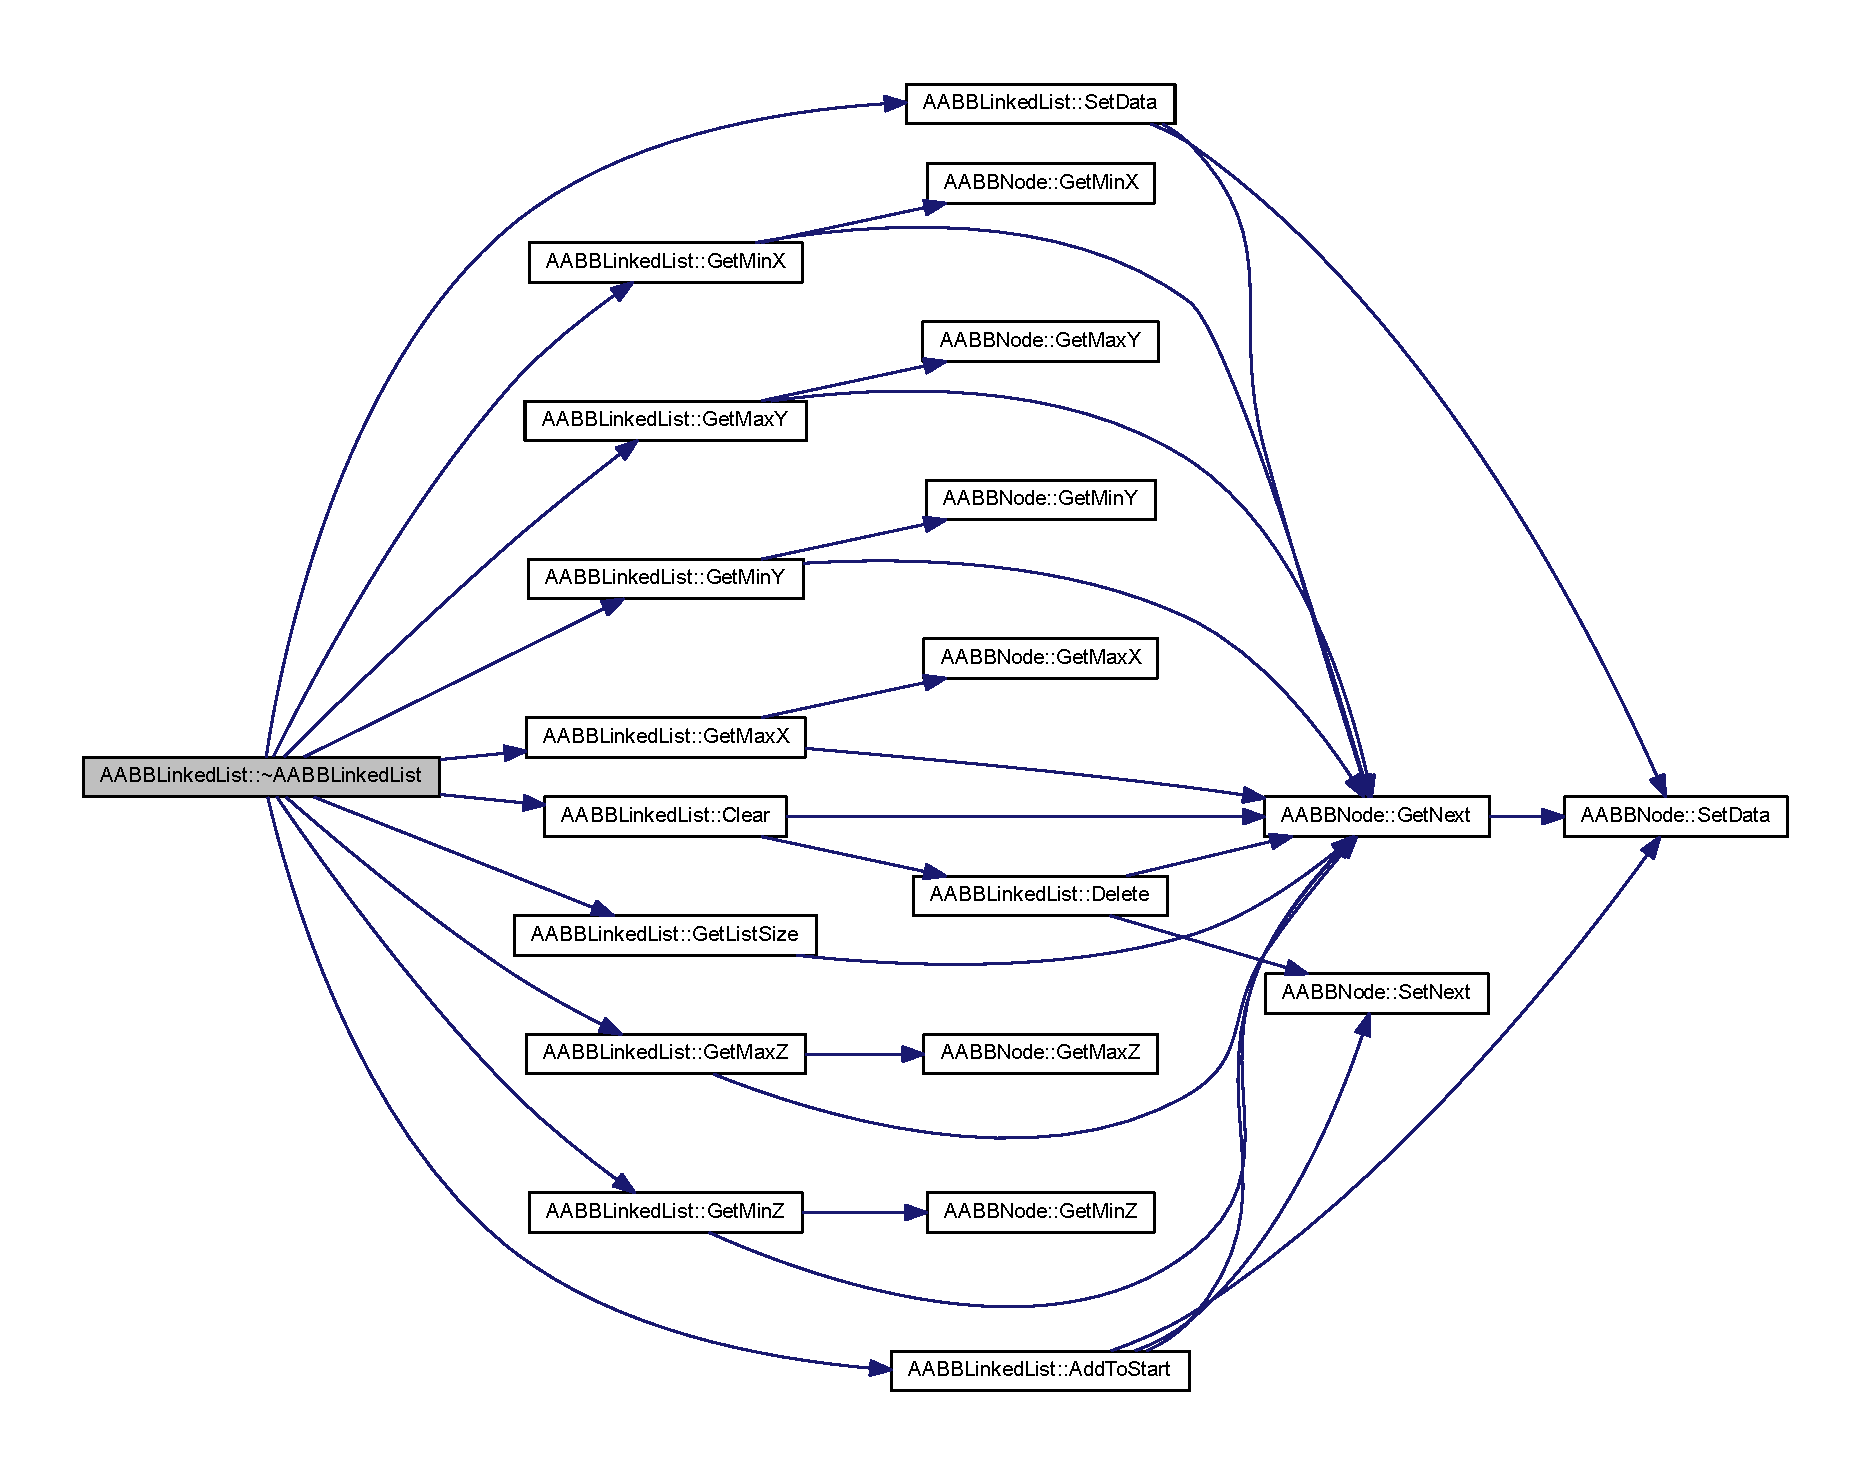
\includegraphics[width=350pt]{class_a_a_b_b_linked_list_a045b677f4cceafb09d188e7a08f5e065_cgraph}
\end{center}
\end{figure}


\index{A\+A\+B\+B\+Linked\+List@{A\+A\+B\+B\+Linked\+List}!A\+A\+B\+B\+Linked\+List@{A\+A\+B\+B\+Linked\+List}}
\index{A\+A\+B\+B\+Linked\+List@{A\+A\+B\+B\+Linked\+List}!A\+A\+B\+B\+Linked\+List@{A\+A\+B\+B\+Linked\+List}}
\subsubsection[{\texorpdfstring{A\+A\+B\+B\+Linked\+List(const A\+A\+B\+B\+Linked\+List \&ll)}{AABBLinkedList(const AABBLinkedList &ll)}}]{\setlength{\rightskip}{0pt plus 5cm}A\+A\+B\+B\+Linked\+List\+::\+A\+A\+B\+B\+Linked\+List (
\begin{DoxyParamCaption}
\item[{const {\bf A\+A\+B\+B\+Linked\+List} \&}]{ll}
\end{DoxyParamCaption}
)\hspace{0.3cm}{\ttfamily [inline]}, {\ttfamily [private]}}\hypertarget{class_a_a_b_b_linked_list_ad59bb13edd2c35799bf927038836ddea}{}\label{class_a_a_b_b_linked_list_ad59bb13edd2c35799bf927038836ddea}


\subsection{Member Function Documentation}
\index{A\+A\+B\+B\+Linked\+List@{A\+A\+B\+B\+Linked\+List}!Add\+To\+Start@{Add\+To\+Start}}
\index{Add\+To\+Start@{Add\+To\+Start}!A\+A\+B\+B\+Linked\+List@{A\+A\+B\+B\+Linked\+List}}
\subsubsection[{\texorpdfstring{Add\+To\+Start(\+G\+Ldouble max\+X, G\+Ldouble min\+X, G\+Ldouble max\+Y, G\+Ldouble min\+Y, G\+Ldouble max\+Z, G\+Ldouble min\+Z)}{AddToStart(GLdouble maxX, GLdouble minX, GLdouble maxY, GLdouble minY, GLdouble maxZ, GLdouble minZ)}}]{\setlength{\rightskip}{0pt plus 5cm}bool A\+A\+B\+B\+Linked\+List\+::\+Add\+To\+Start (
\begin{DoxyParamCaption}
\item[{G\+Ldouble}]{maxX, }
\item[{G\+Ldouble}]{minX, }
\item[{G\+Ldouble}]{maxY, }
\item[{G\+Ldouble}]{minY, }
\item[{G\+Ldouble}]{maxZ, }
\item[{G\+Ldouble}]{minZ}
\end{DoxyParamCaption}
)}\hypertarget{class_a_a_b_b_linked_list_a0dda8d1e7b9d5a2721b518d03b141664}{}\label{class_a_a_b_b_linked_list_a0dda8d1e7b9d5a2721b518d03b141664}


Here is the call graph for this function\+:
\nopagebreak
\begin{figure}[H]
\begin{center}
\leavevmode
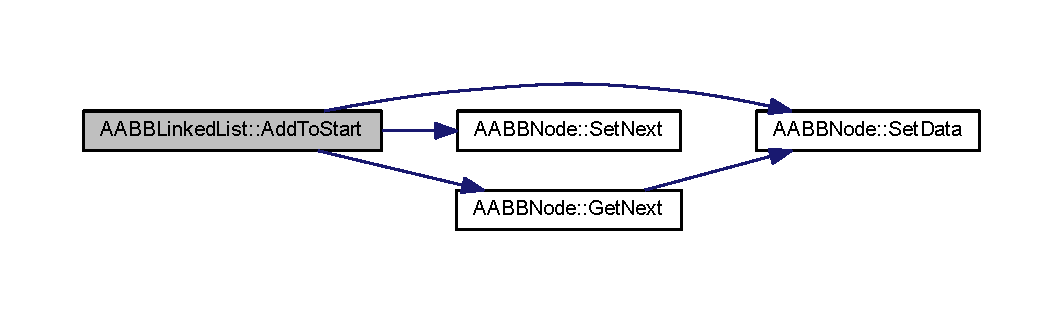
\includegraphics[width=350pt]{class_a_a_b_b_linked_list_a0dda8d1e7b9d5a2721b518d03b141664_cgraph}
\end{center}
\end{figure}




Here is the caller graph for this function\+:
\nopagebreak
\begin{figure}[H]
\begin{center}
\leavevmode
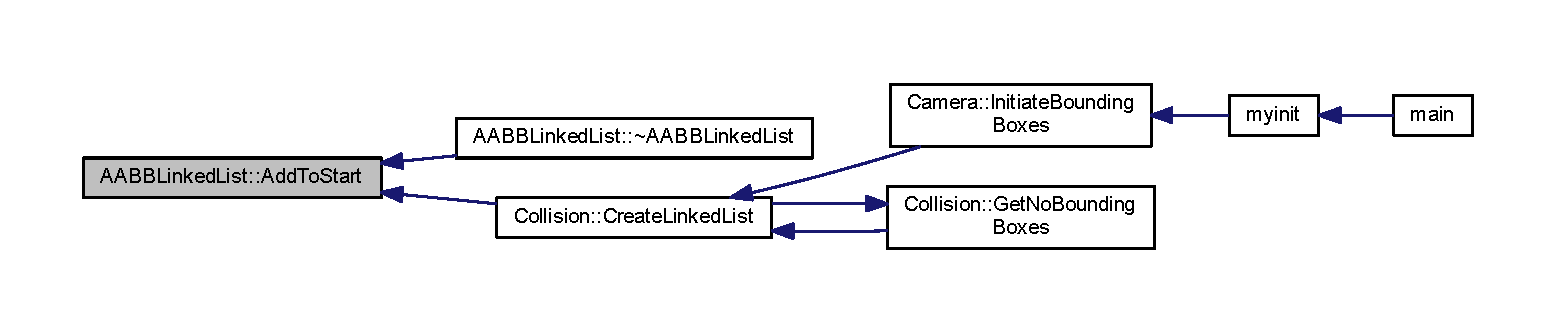
\includegraphics[width=350pt]{class_a_a_b_b_linked_list_a0dda8d1e7b9d5a2721b518d03b141664_icgraph}
\end{center}
\end{figure}


\index{A\+A\+B\+B\+Linked\+List@{A\+A\+B\+B\+Linked\+List}!Clear@{Clear}}
\index{Clear@{Clear}!A\+A\+B\+B\+Linked\+List@{A\+A\+B\+B\+Linked\+List}}
\subsubsection[{\texorpdfstring{Clear()}{Clear()}}]{\setlength{\rightskip}{0pt plus 5cm}void A\+A\+B\+B\+Linked\+List\+::\+Clear (
\begin{DoxyParamCaption}
{}
\end{DoxyParamCaption}
)}\hypertarget{class_a_a_b_b_linked_list_a91220ba141deab9a3da2ec7ca6396436}{}\label{class_a_a_b_b_linked_list_a91220ba141deab9a3da2ec7ca6396436}


Here is the call graph for this function\+:
\nopagebreak
\begin{figure}[H]
\begin{center}
\leavevmode
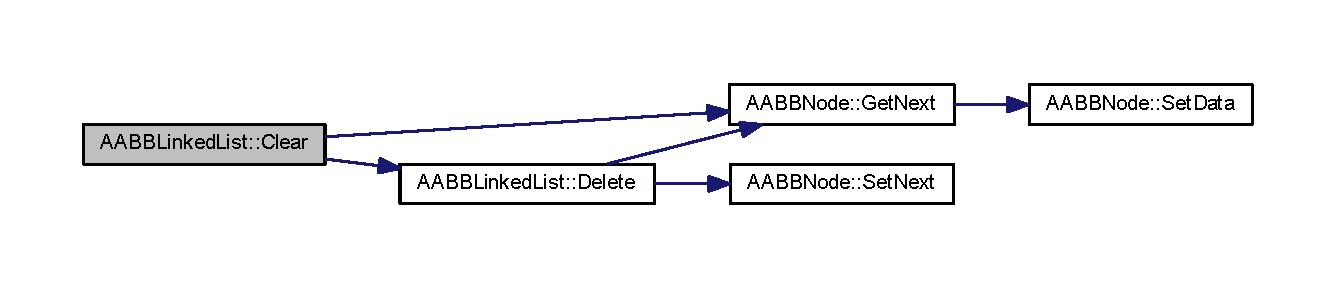
\includegraphics[width=350pt]{class_a_a_b_b_linked_list_a91220ba141deab9a3da2ec7ca6396436_cgraph}
\end{center}
\end{figure}




Here is the caller graph for this function\+:
\nopagebreak
\begin{figure}[H]
\begin{center}
\leavevmode
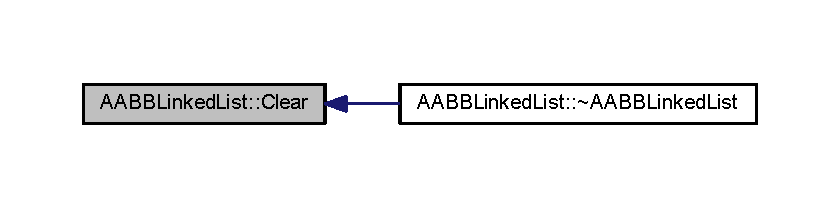
\includegraphics[width=350pt]{class_a_a_b_b_linked_list_a91220ba141deab9a3da2ec7ca6396436_icgraph}
\end{center}
\end{figure}


\index{A\+A\+B\+B\+Linked\+List@{A\+A\+B\+B\+Linked\+List}!Delete@{Delete}}
\index{Delete@{Delete}!A\+A\+B\+B\+Linked\+List@{A\+A\+B\+B\+Linked\+List}}
\subsubsection[{\texorpdfstring{Delete(\+A\+A\+B\+B\+Node $\ast$before)}{Delete(AABBNode *before)}}]{\setlength{\rightskip}{0pt plus 5cm}void A\+A\+B\+B\+Linked\+List\+::\+Delete (
\begin{DoxyParamCaption}
\item[{{\bf A\+A\+B\+B\+Node} $\ast$}]{before}
\end{DoxyParamCaption}
)\hspace{0.3cm}{\ttfamily [private]}}\hypertarget{class_a_a_b_b_linked_list_aa4e4c62a0b374cafb85f5f41a9d31553}{}\label{class_a_a_b_b_linked_list_aa4e4c62a0b374cafb85f5f41a9d31553}


Here is the call graph for this function\+:
\nopagebreak
\begin{figure}[H]
\begin{center}
\leavevmode
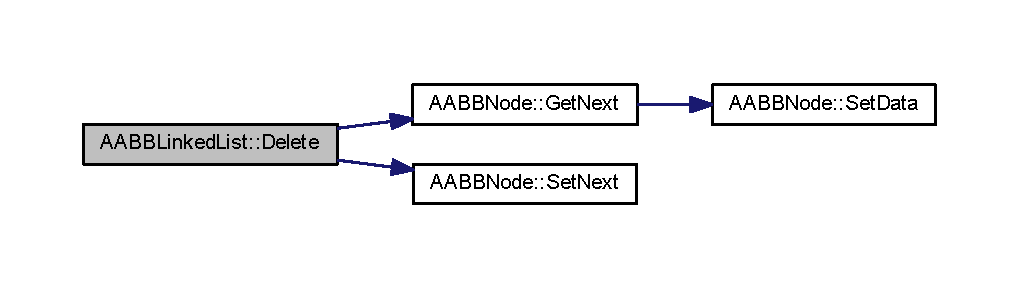
\includegraphics[width=350pt]{class_a_a_b_b_linked_list_aa4e4c62a0b374cafb85f5f41a9d31553_cgraph}
\end{center}
\end{figure}




Here is the caller graph for this function\+:
\nopagebreak
\begin{figure}[H]
\begin{center}
\leavevmode
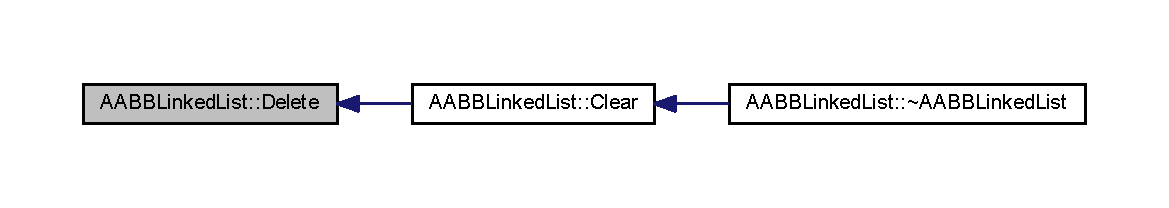
\includegraphics[width=350pt]{class_a_a_b_b_linked_list_aa4e4c62a0b374cafb85f5f41a9d31553_icgraph}
\end{center}
\end{figure}


\index{A\+A\+B\+B\+Linked\+List@{A\+A\+B\+B\+Linked\+List}!Get\+First@{Get\+First}}
\index{Get\+First@{Get\+First}!A\+A\+B\+B\+Linked\+List@{A\+A\+B\+B\+Linked\+List}}
\subsubsection[{\texorpdfstring{Get\+First() const }{GetFirst() const }}]{\setlength{\rightskip}{0pt plus 5cm}{\bf A\+A\+B\+B\+Node}$\ast$ A\+A\+B\+B\+Linked\+List\+::\+Get\+First (
\begin{DoxyParamCaption}
{}
\end{DoxyParamCaption}
) const\hspace{0.3cm}{\ttfamily [inline]}}\hypertarget{class_a_a_b_b_linked_list_a51b92571c3e95ca4b3906a8a6aae547f}{}\label{class_a_a_b_b_linked_list_a51b92571c3e95ca4b3906a8a6aae547f}
\index{A\+A\+B\+B\+Linked\+List@{A\+A\+B\+B\+Linked\+List}!Get\+List\+Size@{Get\+List\+Size}}
\index{Get\+List\+Size@{Get\+List\+Size}!A\+A\+B\+B\+Linked\+List@{A\+A\+B\+B\+Linked\+List}}
\subsubsection[{\texorpdfstring{Get\+List\+Size()}{GetListSize()}}]{\setlength{\rightskip}{0pt plus 5cm}int A\+A\+B\+B\+Linked\+List\+::\+Get\+List\+Size (
\begin{DoxyParamCaption}
{}
\end{DoxyParamCaption}
)}\hypertarget{class_a_a_b_b_linked_list_a42ebbd212e1058adab56b5829dedffca}{}\label{class_a_a_b_b_linked_list_a42ebbd212e1058adab56b5829dedffca}


Here is the call graph for this function\+:
\nopagebreak
\begin{figure}[H]
\begin{center}
\leavevmode
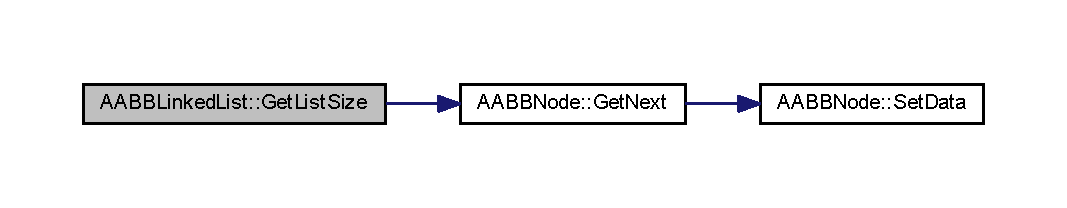
\includegraphics[width=350pt]{class_a_a_b_b_linked_list_a42ebbd212e1058adab56b5829dedffca_cgraph}
\end{center}
\end{figure}




Here is the caller graph for this function\+:
\nopagebreak
\begin{figure}[H]
\begin{center}
\leavevmode
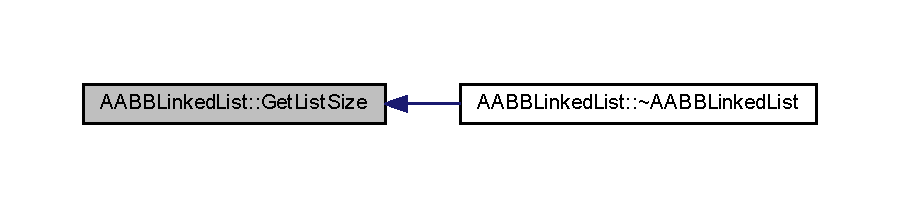
\includegraphics[width=350pt]{class_a_a_b_b_linked_list_a42ebbd212e1058adab56b5829dedffca_icgraph}
\end{center}
\end{figure}


\index{A\+A\+B\+B\+Linked\+List@{A\+A\+B\+B\+Linked\+List}!Get\+MaxX@{Get\+MaxX}}
\index{Get\+MaxX@{Get\+MaxX}!A\+A\+B\+B\+Linked\+List@{A\+A\+B\+B\+Linked\+List}}
\subsubsection[{\texorpdfstring{Get\+Max\+X(int ptr\+Count)}{GetMaxX(int ptrCount)}}]{\setlength{\rightskip}{0pt plus 5cm}G\+Ldouble A\+A\+B\+B\+Linked\+List\+::\+Get\+MaxX (
\begin{DoxyParamCaption}
\item[{int}]{ptr\+Count}
\end{DoxyParamCaption}
)}\hypertarget{class_a_a_b_b_linked_list_a8e5dfc22a5b09a5439c7d48c777f21b6}{}\label{class_a_a_b_b_linked_list_a8e5dfc22a5b09a5439c7d48c777f21b6}


Here is the call graph for this function\+:
\nopagebreak
\begin{figure}[H]
\begin{center}
\leavevmode
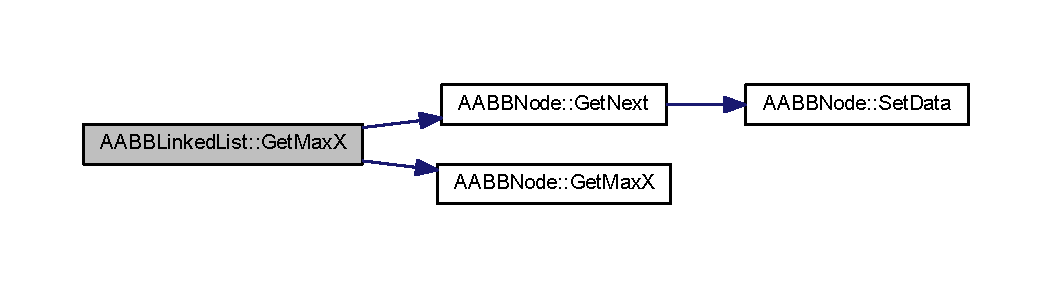
\includegraphics[width=350pt]{class_a_a_b_b_linked_list_a8e5dfc22a5b09a5439c7d48c777f21b6_cgraph}
\end{center}
\end{figure}




Here is the caller graph for this function\+:
\nopagebreak
\begin{figure}[H]
\begin{center}
\leavevmode
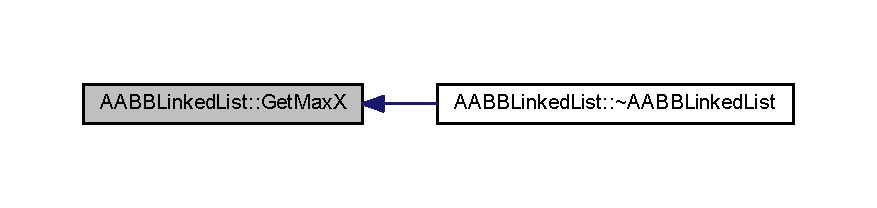
\includegraphics[width=350pt]{class_a_a_b_b_linked_list_a8e5dfc22a5b09a5439c7d48c777f21b6_icgraph}
\end{center}
\end{figure}


\index{A\+A\+B\+B\+Linked\+List@{A\+A\+B\+B\+Linked\+List}!Get\+MaxY@{Get\+MaxY}}
\index{Get\+MaxY@{Get\+MaxY}!A\+A\+B\+B\+Linked\+List@{A\+A\+B\+B\+Linked\+List}}
\subsubsection[{\texorpdfstring{Get\+Max\+Y(int ptr\+Count)}{GetMaxY(int ptrCount)}}]{\setlength{\rightskip}{0pt plus 5cm}G\+Ldouble A\+A\+B\+B\+Linked\+List\+::\+Get\+MaxY (
\begin{DoxyParamCaption}
\item[{int}]{ptr\+Count}
\end{DoxyParamCaption}
)}\hypertarget{class_a_a_b_b_linked_list_a06e37c604e86a670fc6657aac7ada31b}{}\label{class_a_a_b_b_linked_list_a06e37c604e86a670fc6657aac7ada31b}


Here is the call graph for this function\+:
\nopagebreak
\begin{figure}[H]
\begin{center}
\leavevmode
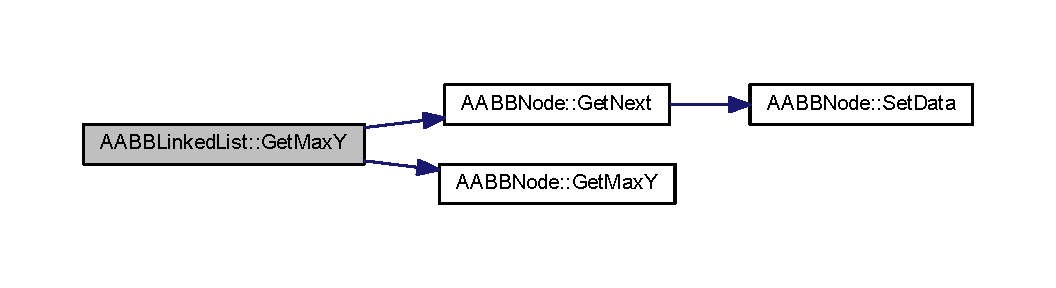
\includegraphics[width=350pt]{class_a_a_b_b_linked_list_a06e37c604e86a670fc6657aac7ada31b_cgraph}
\end{center}
\end{figure}




Here is the caller graph for this function\+:
\nopagebreak
\begin{figure}[H]
\begin{center}
\leavevmode
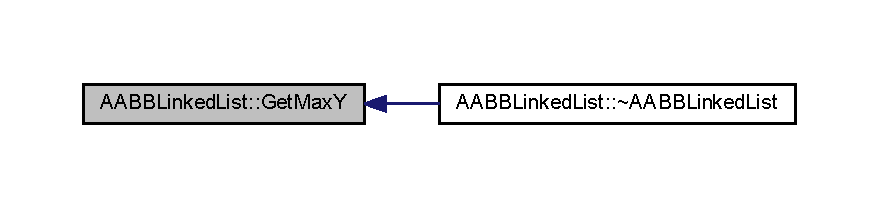
\includegraphics[width=350pt]{class_a_a_b_b_linked_list_a06e37c604e86a670fc6657aac7ada31b_icgraph}
\end{center}
\end{figure}


\index{A\+A\+B\+B\+Linked\+List@{A\+A\+B\+B\+Linked\+List}!Get\+MaxZ@{Get\+MaxZ}}
\index{Get\+MaxZ@{Get\+MaxZ}!A\+A\+B\+B\+Linked\+List@{A\+A\+B\+B\+Linked\+List}}
\subsubsection[{\texorpdfstring{Get\+Max\+Z(int ptr\+Count)}{GetMaxZ(int ptrCount)}}]{\setlength{\rightskip}{0pt plus 5cm}G\+Ldouble A\+A\+B\+B\+Linked\+List\+::\+Get\+MaxZ (
\begin{DoxyParamCaption}
\item[{int}]{ptr\+Count}
\end{DoxyParamCaption}
)}\hypertarget{class_a_a_b_b_linked_list_af728cb9e63fe37667356ec4a74d9bb09}{}\label{class_a_a_b_b_linked_list_af728cb9e63fe37667356ec4a74d9bb09}


Here is the call graph for this function\+:
\nopagebreak
\begin{figure}[H]
\begin{center}
\leavevmode
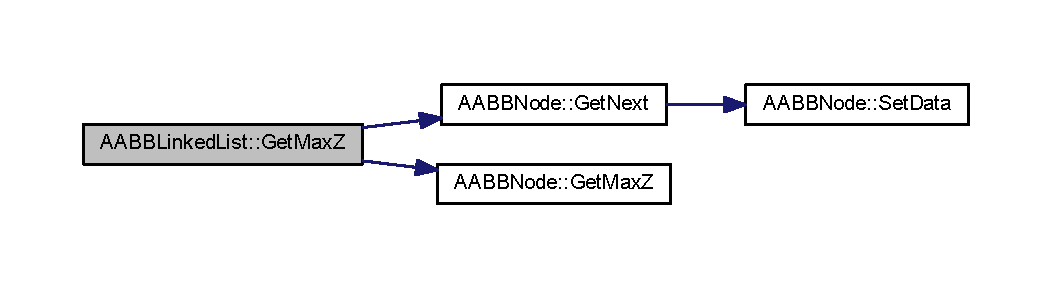
\includegraphics[width=350pt]{class_a_a_b_b_linked_list_af728cb9e63fe37667356ec4a74d9bb09_cgraph}
\end{center}
\end{figure}




Here is the caller graph for this function\+:
\nopagebreak
\begin{figure}[H]
\begin{center}
\leavevmode
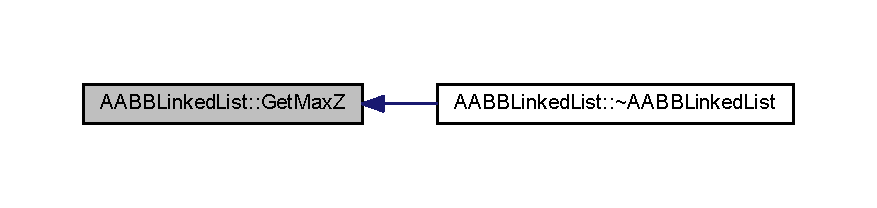
\includegraphics[width=350pt]{class_a_a_b_b_linked_list_af728cb9e63fe37667356ec4a74d9bb09_icgraph}
\end{center}
\end{figure}


\index{A\+A\+B\+B\+Linked\+List@{A\+A\+B\+B\+Linked\+List}!Get\+MinX@{Get\+MinX}}
\index{Get\+MinX@{Get\+MinX}!A\+A\+B\+B\+Linked\+List@{A\+A\+B\+B\+Linked\+List}}
\subsubsection[{\texorpdfstring{Get\+Min\+X(int ptr\+Count)}{GetMinX(int ptrCount)}}]{\setlength{\rightskip}{0pt plus 5cm}G\+Ldouble A\+A\+B\+B\+Linked\+List\+::\+Get\+MinX (
\begin{DoxyParamCaption}
\item[{int}]{ptr\+Count}
\end{DoxyParamCaption}
)}\hypertarget{class_a_a_b_b_linked_list_a01b738ef73d102240bc9bd54044c2a46}{}\label{class_a_a_b_b_linked_list_a01b738ef73d102240bc9bd54044c2a46}


Here is the call graph for this function\+:
\nopagebreak
\begin{figure}[H]
\begin{center}
\leavevmode
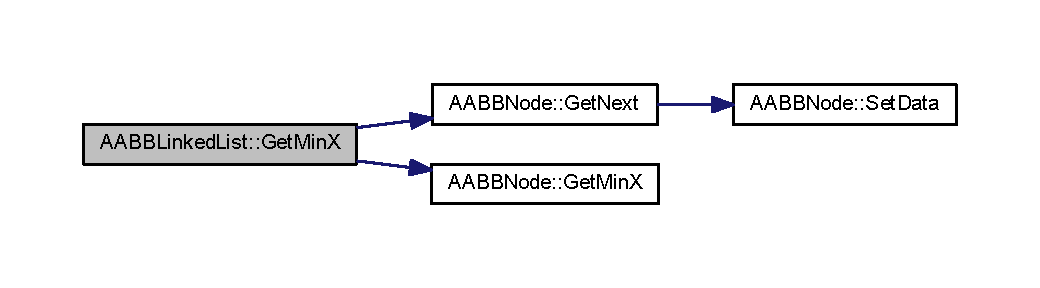
\includegraphics[width=350pt]{class_a_a_b_b_linked_list_a01b738ef73d102240bc9bd54044c2a46_cgraph}
\end{center}
\end{figure}




Here is the caller graph for this function\+:
\nopagebreak
\begin{figure}[H]
\begin{center}
\leavevmode
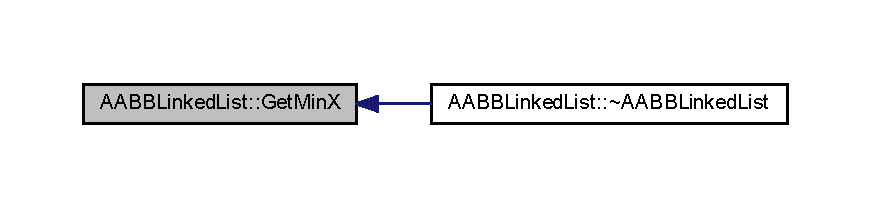
\includegraphics[width=350pt]{class_a_a_b_b_linked_list_a01b738ef73d102240bc9bd54044c2a46_icgraph}
\end{center}
\end{figure}


\index{A\+A\+B\+B\+Linked\+List@{A\+A\+B\+B\+Linked\+List}!Get\+MinY@{Get\+MinY}}
\index{Get\+MinY@{Get\+MinY}!A\+A\+B\+B\+Linked\+List@{A\+A\+B\+B\+Linked\+List}}
\subsubsection[{\texorpdfstring{Get\+Min\+Y(int ptr\+Count)}{GetMinY(int ptrCount)}}]{\setlength{\rightskip}{0pt plus 5cm}G\+Ldouble A\+A\+B\+B\+Linked\+List\+::\+Get\+MinY (
\begin{DoxyParamCaption}
\item[{int}]{ptr\+Count}
\end{DoxyParamCaption}
)}\hypertarget{class_a_a_b_b_linked_list_aa59cbdbfb2012f733010283639a27584}{}\label{class_a_a_b_b_linked_list_aa59cbdbfb2012f733010283639a27584}


Here is the call graph for this function\+:
\nopagebreak
\begin{figure}[H]
\begin{center}
\leavevmode
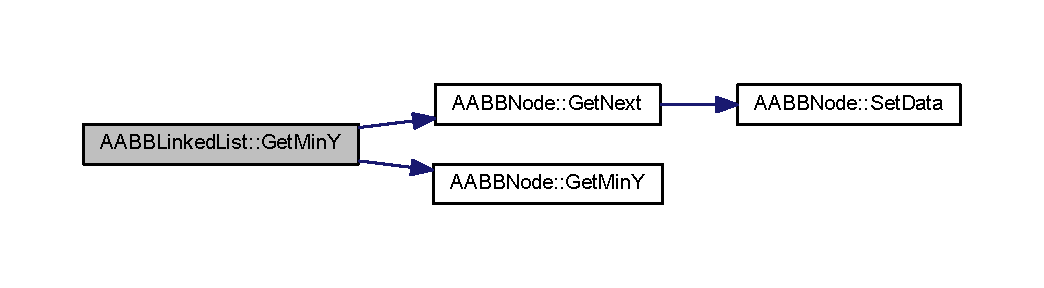
\includegraphics[width=350pt]{class_a_a_b_b_linked_list_aa59cbdbfb2012f733010283639a27584_cgraph}
\end{center}
\end{figure}




Here is the caller graph for this function\+:
\nopagebreak
\begin{figure}[H]
\begin{center}
\leavevmode
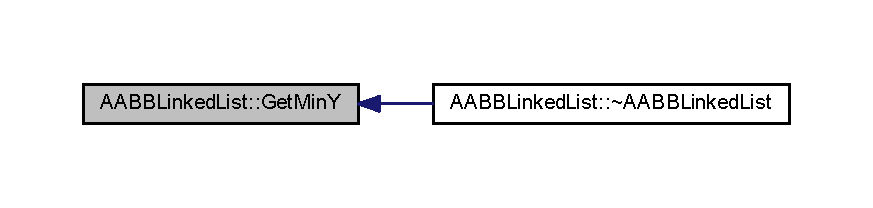
\includegraphics[width=350pt]{class_a_a_b_b_linked_list_aa59cbdbfb2012f733010283639a27584_icgraph}
\end{center}
\end{figure}


\index{A\+A\+B\+B\+Linked\+List@{A\+A\+B\+B\+Linked\+List}!Get\+MinZ@{Get\+MinZ}}
\index{Get\+MinZ@{Get\+MinZ}!A\+A\+B\+B\+Linked\+List@{A\+A\+B\+B\+Linked\+List}}
\subsubsection[{\texorpdfstring{Get\+Min\+Z(int ptr\+Count)}{GetMinZ(int ptrCount)}}]{\setlength{\rightskip}{0pt plus 5cm}G\+Ldouble A\+A\+B\+B\+Linked\+List\+::\+Get\+MinZ (
\begin{DoxyParamCaption}
\item[{int}]{ptr\+Count}
\end{DoxyParamCaption}
)}\hypertarget{class_a_a_b_b_linked_list_a93270a86be1d2f63aca450f7ef39d130}{}\label{class_a_a_b_b_linked_list_a93270a86be1d2f63aca450f7ef39d130}


Here is the call graph for this function\+:
\nopagebreak
\begin{figure}[H]
\begin{center}
\leavevmode
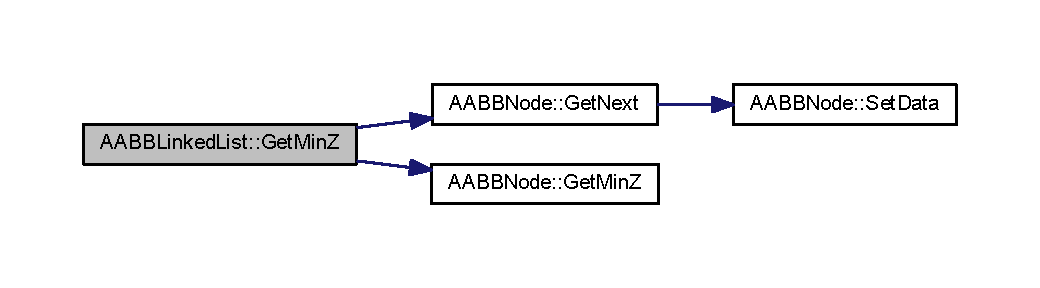
\includegraphics[width=350pt]{class_a_a_b_b_linked_list_a93270a86be1d2f63aca450f7ef39d130_cgraph}
\end{center}
\end{figure}




Here is the caller graph for this function\+:
\nopagebreak
\begin{figure}[H]
\begin{center}
\leavevmode
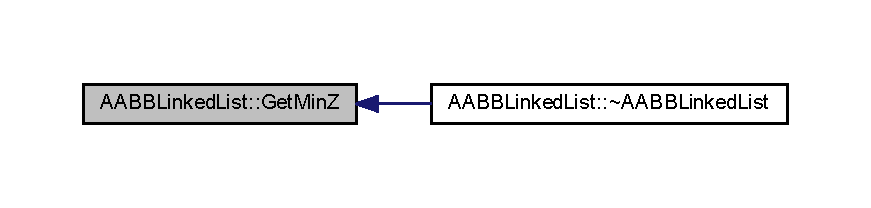
\includegraphics[width=350pt]{class_a_a_b_b_linked_list_a93270a86be1d2f63aca450f7ef39d130_icgraph}
\end{center}
\end{figure}


\index{A\+A\+B\+B\+Linked\+List@{A\+A\+B\+B\+Linked\+List}!Get\+Next@{Get\+Next}}
\index{Get\+Next@{Get\+Next}!A\+A\+B\+B\+Linked\+List@{A\+A\+B\+B\+Linked\+List}}
\subsubsection[{\texorpdfstring{Get\+Next() const }{GetNext() const }}]{\setlength{\rightskip}{0pt plus 5cm}{\bf A\+A\+B\+B\+Node}$\ast$ A\+A\+B\+B\+Linked\+List\+::\+Get\+Next (
\begin{DoxyParamCaption}
{}
\end{DoxyParamCaption}
) const\hspace{0.3cm}{\ttfamily [inline]}}\hypertarget{class_a_a_b_b_linked_list_a8843e719c2db1f73087fe772a39fa1af}{}\label{class_a_a_b_b_linked_list_a8843e719c2db1f73087fe772a39fa1af}


Here is the call graph for this function\+:
\nopagebreak
\begin{figure}[H]
\begin{center}
\leavevmode
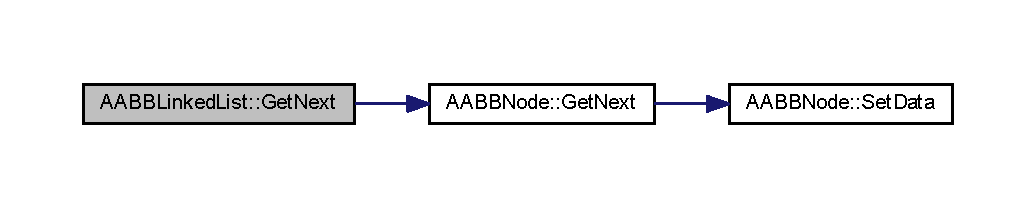
\includegraphics[width=350pt]{class_a_a_b_b_linked_list_a8843e719c2db1f73087fe772a39fa1af_cgraph}
\end{center}
\end{figure}


\index{A\+A\+B\+B\+Linked\+List@{A\+A\+B\+B\+Linked\+List}!operator=@{operator=}}
\index{operator=@{operator=}!A\+A\+B\+B\+Linked\+List@{A\+A\+B\+B\+Linked\+List}}
\subsubsection[{\texorpdfstring{operator=(const A\+A\+B\+B\+Linked\+List \&ll)}{operator=(const AABBLinkedList &ll)}}]{\setlength{\rightskip}{0pt plus 5cm}{\bf A\+A\+B\+B\+Linked\+List}\& A\+A\+B\+B\+Linked\+List\+::operator= (
\begin{DoxyParamCaption}
\item[{const {\bf A\+A\+B\+B\+Linked\+List} \&}]{ll}
\end{DoxyParamCaption}
)\hspace{0.3cm}{\ttfamily [inline]}, {\ttfamily [private]}}\hypertarget{class_a_a_b_b_linked_list_ac70cf6e12aba18c1245566e226199d3d}{}\label{class_a_a_b_b_linked_list_ac70cf6e12aba18c1245566e226199d3d}
\index{A\+A\+B\+B\+Linked\+List@{A\+A\+B\+B\+Linked\+List}!Set\+Data@{Set\+Data}}
\index{Set\+Data@{Set\+Data}!A\+A\+B\+B\+Linked\+List@{A\+A\+B\+B\+Linked\+List}}
\subsubsection[{\texorpdfstring{Set\+Data(const int \&ptr\+Count, const G\+Ldouble max\+X, const G\+Ldouble min\+X, const G\+Ldouble max\+Y, const G\+Ldouble min\+Y, const G\+Ldouble max\+Z, const G\+Ldouble min\+Z)}{SetData(const int &ptrCount, const GLdouble maxX, const GLdouble minX, const GLdouble maxY, const GLdouble minY, const GLdouble maxZ, const GLdouble minZ)}}]{\setlength{\rightskip}{0pt plus 5cm}void A\+A\+B\+B\+Linked\+List\+::\+Set\+Data (
\begin{DoxyParamCaption}
\item[{const int \&}]{ptr\+Count, }
\item[{const G\+Ldouble}]{maxX, }
\item[{const G\+Ldouble}]{minX, }
\item[{const G\+Ldouble}]{maxY, }
\item[{const G\+Ldouble}]{minY, }
\item[{const G\+Ldouble}]{maxZ, }
\item[{const G\+Ldouble}]{minZ}
\end{DoxyParamCaption}
)}\hypertarget{class_a_a_b_b_linked_list_a9466a3aaffb597d9976259726b44463a}{}\label{class_a_a_b_b_linked_list_a9466a3aaffb597d9976259726b44463a}


Here is the call graph for this function\+:
\nopagebreak
\begin{figure}[H]
\begin{center}
\leavevmode
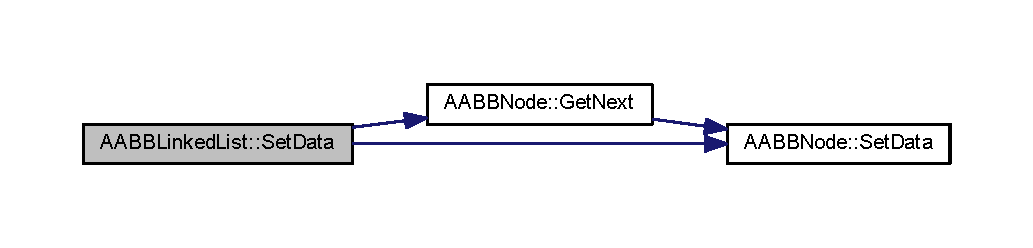
\includegraphics[width=350pt]{class_a_a_b_b_linked_list_a9466a3aaffb597d9976259726b44463a_cgraph}
\end{center}
\end{figure}




Here is the caller graph for this function\+:
\nopagebreak
\begin{figure}[H]
\begin{center}
\leavevmode
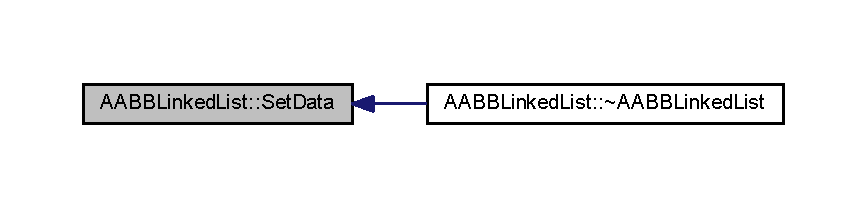
\includegraphics[width=350pt]{class_a_a_b_b_linked_list_a9466a3aaffb597d9976259726b44463a_icgraph}
\end{center}
\end{figure}




\subsection{Member Data Documentation}
\index{A\+A\+B\+B\+Linked\+List@{A\+A\+B\+B\+Linked\+List}!m\+\_\+first@{m\+\_\+first}}
\index{m\+\_\+first@{m\+\_\+first}!A\+A\+B\+B\+Linked\+List@{A\+A\+B\+B\+Linked\+List}}
\subsubsection[{\texorpdfstring{m\+\_\+first}{m_first}}]{\setlength{\rightskip}{0pt plus 5cm}{\bf A\+A\+B\+B\+Node}$\ast$ A\+A\+B\+B\+Linked\+List\+::m\+\_\+first\hspace{0.3cm}{\ttfamily [private]}}\hypertarget{class_a_a_b_b_linked_list_ae5641ef70823a45200dc68b28bf47351}{}\label{class_a_a_b_b_linked_list_ae5641ef70823a45200dc68b28bf47351}


The documentation for this class was generated from the following files\+:\begin{DoxyCompactItemize}
\item 
C\+:/000\+Uniwork/\+I\+C\+T290 Games Programming Try 2/\+Exercise 1/\+C\+A\+M\+P\+U\+S T\+O\+U\+R/\hyperlink{_a_a_b_b_linked_list_8h}{A\+A\+B\+B\+Linked\+List.\+h}\item 
C\+:/000\+Uniwork/\+I\+C\+T290 Games Programming Try 2/\+Exercise 1/\+C\+A\+M\+P\+U\+S T\+O\+U\+R/\hyperlink{_a_a_b_b_linked_list_8cpp}{A\+A\+B\+B\+Linked\+List.\+cpp}\end{DoxyCompactItemize}

\hypertarget{class_a_a_b_b_node}{}\section{A\+A\+B\+B\+Node Class Reference}
\label{class_a_a_b_b_node}\index{A\+A\+B\+B\+Node@{A\+A\+B\+B\+Node}}


{\ttfamily \#include $<$A\+A\+B\+B\+Node.\+h$>$}



Collaboration diagram for A\+A\+B\+B\+Node\+:
\nopagebreak
\begin{figure}[H]
\begin{center}
\leavevmode
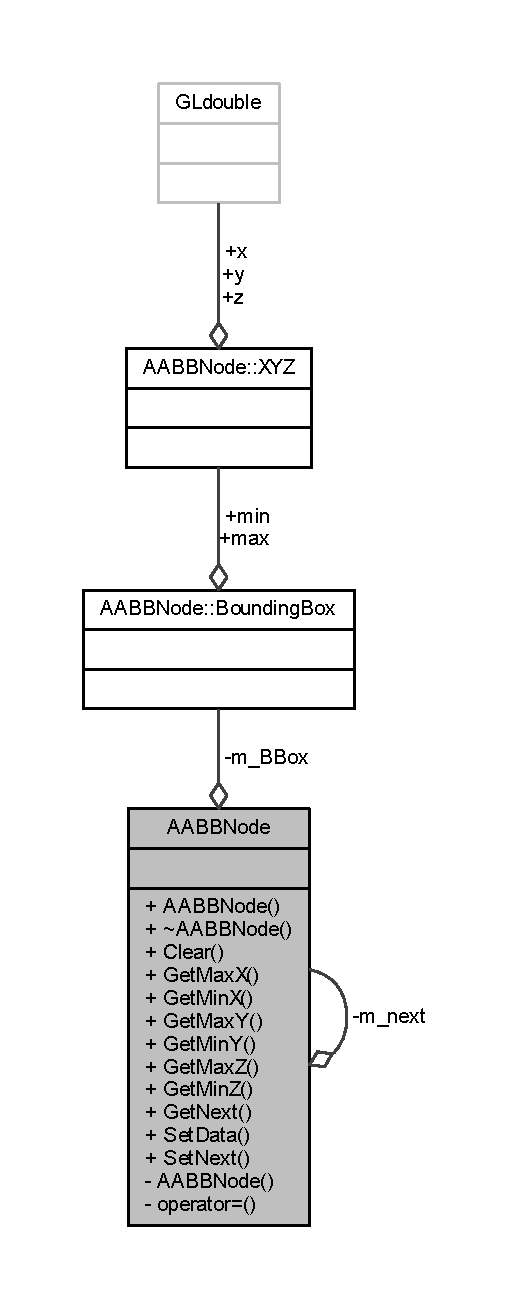
\includegraphics[height=550pt]{class_a_a_b_b_node__coll__graph}
\end{center}
\end{figure}
\subsection*{Classes}
\begin{DoxyCompactItemize}
\item 
struct \hyperlink{struct_a_a_b_b_node_1_1_bounding_box}{Bounding\+Box}
\item 
struct \hyperlink{struct_a_a_b_b_node_1_1_x_y_z}{X\+YZ}
\end{DoxyCompactItemize}
\subsection*{Public Member Functions}
\begin{DoxyCompactItemize}
\item 
\hyperlink{class_a_a_b_b_node_ab44974b730878548779dcc724b8a5be7}{A\+A\+B\+B\+Node} ()
\item 
virtual \hyperlink{class_a_a_b_b_node_a9836982140490a8e86a9822dbc0d53e6}{$\sim$\+A\+A\+B\+B\+Node} ()
\item 
void \hyperlink{class_a_a_b_b_node_a1b1bafc601218c6b5870e430998e387f}{Clear} ()
\item 
G\+Ldouble \hyperlink{class_a_a_b_b_node_adb707da6d39fdae8230dd40f33a6cc85}{Get\+MaxX} ()
\item 
G\+Ldouble \hyperlink{class_a_a_b_b_node_ada7009629434897aefb2b58384ae91e2}{Get\+MinX} ()
\item 
G\+Ldouble \hyperlink{class_a_a_b_b_node_aca46418ff41fbadd321474617abe81e8}{Get\+MaxY} ()
\item 
G\+Ldouble \hyperlink{class_a_a_b_b_node_a1dfa67f00ed2e48487df020eb5a20fd0}{Get\+MinY} ()
\item 
G\+Ldouble \hyperlink{class_a_a_b_b_node_a86f9e03ef5e39913c520b00dd06541e6}{Get\+MaxZ} ()
\item 
G\+Ldouble \hyperlink{class_a_a_b_b_node_a9d8ab82f585a852cc45cb1d8b27188cf}{Get\+MinZ} ()
\item 
\hyperlink{class_a_a_b_b_node}{A\+A\+B\+B\+Node} $\ast$ \hyperlink{class_a_a_b_b_node_aeba066c64653e3a9d73e0b617a8b844c}{Get\+Next} () const 
\item 
void \hyperlink{class_a_a_b_b_node_a43c049985e68d0d7443dc7ba11c71979}{Set\+Data} (const G\+Ldouble maxX, const G\+Ldouble minX, const G\+Ldouble maxY, const G\+Ldouble minY, const G\+Ldouble maxZ, const G\+Ldouble minZ)
\item 
void \hyperlink{class_a_a_b_b_node_a2d624ad9c1241156af7a4dd96cbcd40f}{Set\+Next} (\hyperlink{class_a_a_b_b_node}{A\+A\+B\+B\+Node} $\ast$next)
\end{DoxyCompactItemize}
\subsection*{Private Member Functions}
\begin{DoxyCompactItemize}
\item 
\hyperlink{class_a_a_b_b_node_ae5599cabd1c7ff4437d979ba52c487f6}{A\+A\+B\+B\+Node} (const \hyperlink{class_a_a_b_b_node}{A\+A\+B\+B\+Node} \&new\+Node)
\item 
\hyperlink{class_a_a_b_b_node}{A\+A\+B\+B\+Node} \& \hyperlink{class_a_a_b_b_node_aa4302db47c66af98472bcf6f42c6ba65}{operator=} (const \hyperlink{class_a_a_b_b_node}{A\+A\+B\+B\+Node} \&new\+Node)
\end{DoxyCompactItemize}
\subsection*{Private Attributes}
\begin{DoxyCompactItemize}
\item 
\hyperlink{class_a_a_b_b_node}{A\+A\+B\+B\+Node} $\ast$ \hyperlink{class_a_a_b_b_node_a2fe0e4624db458571d0935f4b09ec415}{m\+\_\+next}
\item 
\hyperlink{struct_a_a_b_b_node_1_1_bounding_box}{Bounding\+Box} \hyperlink{class_a_a_b_b_node_ac45482982e70ba3d40c2099b99db0663}{m\+\_\+\+B\+Box}
\end{DoxyCompactItemize}


\subsection{Constructor \& Destructor Documentation}
\index{A\+A\+B\+B\+Node@{A\+A\+B\+B\+Node}!A\+A\+B\+B\+Node@{A\+A\+B\+B\+Node}}
\index{A\+A\+B\+B\+Node@{A\+A\+B\+B\+Node}!A\+A\+B\+B\+Node@{A\+A\+B\+B\+Node}}
\subsubsection[{\texorpdfstring{A\+A\+B\+B\+Node()}{AABBNode()}}]{\setlength{\rightskip}{0pt plus 5cm}A\+A\+B\+B\+Node\+::\+A\+A\+B\+B\+Node (
\begin{DoxyParamCaption}
{}
\end{DoxyParamCaption}
)\hspace{0.3cm}{\ttfamily [inline]}}\hypertarget{class_a_a_b_b_node_ab44974b730878548779dcc724b8a5be7}{}\label{class_a_a_b_b_node_ab44974b730878548779dcc724b8a5be7}


Here is the call graph for this function\+:
\nopagebreak
\begin{figure}[H]
\begin{center}
\leavevmode
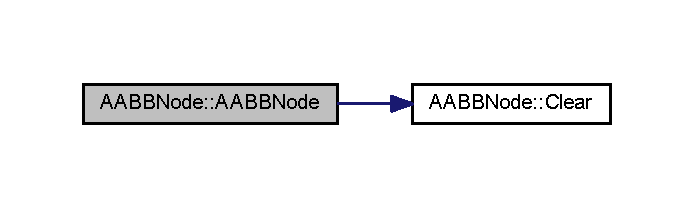
\includegraphics[width=333pt]{class_a_a_b_b_node_ab44974b730878548779dcc724b8a5be7_cgraph}
\end{center}
\end{figure}


\index{A\+A\+B\+B\+Node@{A\+A\+B\+B\+Node}!````~A\+A\+B\+B\+Node@{$\sim$\+A\+A\+B\+B\+Node}}
\index{````~A\+A\+B\+B\+Node@{$\sim$\+A\+A\+B\+B\+Node}!A\+A\+B\+B\+Node@{A\+A\+B\+B\+Node}}
\subsubsection[{\texorpdfstring{$\sim$\+A\+A\+B\+B\+Node()}{~AABBNode()}}]{\setlength{\rightskip}{0pt plus 5cm}virtual A\+A\+B\+B\+Node\+::$\sim$\+A\+A\+B\+B\+Node (
\begin{DoxyParamCaption}
{}
\end{DoxyParamCaption}
)\hspace{0.3cm}{\ttfamily [inline]}, {\ttfamily [virtual]}}\hypertarget{class_a_a_b_b_node_a9836982140490a8e86a9822dbc0d53e6}{}\label{class_a_a_b_b_node_a9836982140490a8e86a9822dbc0d53e6}


Here is the call graph for this function\+:
\nopagebreak
\begin{figure}[H]
\begin{center}
\leavevmode
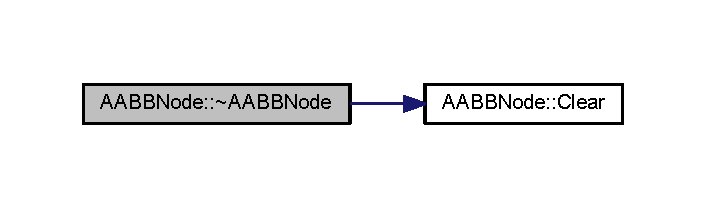
\includegraphics[width=339pt]{class_a_a_b_b_node_a9836982140490a8e86a9822dbc0d53e6_cgraph}
\end{center}
\end{figure}


\index{A\+A\+B\+B\+Node@{A\+A\+B\+B\+Node}!A\+A\+B\+B\+Node@{A\+A\+B\+B\+Node}}
\index{A\+A\+B\+B\+Node@{A\+A\+B\+B\+Node}!A\+A\+B\+B\+Node@{A\+A\+B\+B\+Node}}
\subsubsection[{\texorpdfstring{A\+A\+B\+B\+Node(const A\+A\+B\+B\+Node \&new\+Node)}{AABBNode(const AABBNode &newNode)}}]{\setlength{\rightskip}{0pt plus 5cm}A\+A\+B\+B\+Node\+::\+A\+A\+B\+B\+Node (
\begin{DoxyParamCaption}
\item[{const {\bf A\+A\+B\+B\+Node} \&}]{new\+Node}
\end{DoxyParamCaption}
)\hspace{0.3cm}{\ttfamily [inline]}, {\ttfamily [private]}}\hypertarget{class_a_a_b_b_node_ae5599cabd1c7ff4437d979ba52c487f6}{}\label{class_a_a_b_b_node_ae5599cabd1c7ff4437d979ba52c487f6}


\subsection{Member Function Documentation}
\index{A\+A\+B\+B\+Node@{A\+A\+B\+B\+Node}!Clear@{Clear}}
\index{Clear@{Clear}!A\+A\+B\+B\+Node@{A\+A\+B\+B\+Node}}
\subsubsection[{\texorpdfstring{Clear()}{Clear()}}]{\setlength{\rightskip}{0pt plus 5cm}void A\+A\+B\+B\+Node\+::\+Clear (
\begin{DoxyParamCaption}
{}
\end{DoxyParamCaption}
)}\hypertarget{class_a_a_b_b_node_a1b1bafc601218c6b5870e430998e387f}{}\label{class_a_a_b_b_node_a1b1bafc601218c6b5870e430998e387f}


Here is the caller graph for this function\+:
\nopagebreak
\begin{figure}[H]
\begin{center}
\leavevmode
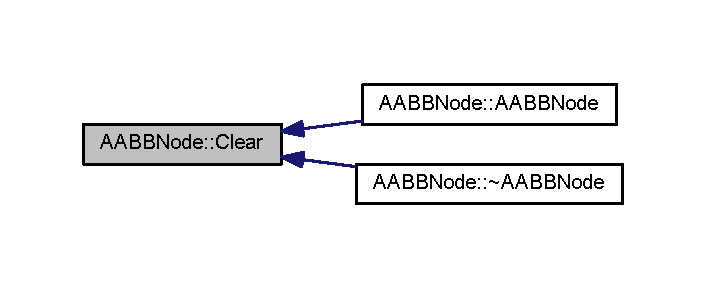
\includegraphics[width=339pt]{class_a_a_b_b_node_a1b1bafc601218c6b5870e430998e387f_icgraph}
\end{center}
\end{figure}


\index{A\+A\+B\+B\+Node@{A\+A\+B\+B\+Node}!Get\+MaxX@{Get\+MaxX}}
\index{Get\+MaxX@{Get\+MaxX}!A\+A\+B\+B\+Node@{A\+A\+B\+B\+Node}}
\subsubsection[{\texorpdfstring{Get\+Max\+X()}{GetMaxX()}}]{\setlength{\rightskip}{0pt plus 5cm}G\+Ldouble A\+A\+B\+B\+Node\+::\+Get\+MaxX (
\begin{DoxyParamCaption}
{}
\end{DoxyParamCaption}
)\hspace{0.3cm}{\ttfamily [inline]}}\hypertarget{class_a_a_b_b_node_adb707da6d39fdae8230dd40f33a6cc85}{}\label{class_a_a_b_b_node_adb707da6d39fdae8230dd40f33a6cc85}


Here is the caller graph for this function\+:
\nopagebreak
\begin{figure}[H]
\begin{center}
\leavevmode
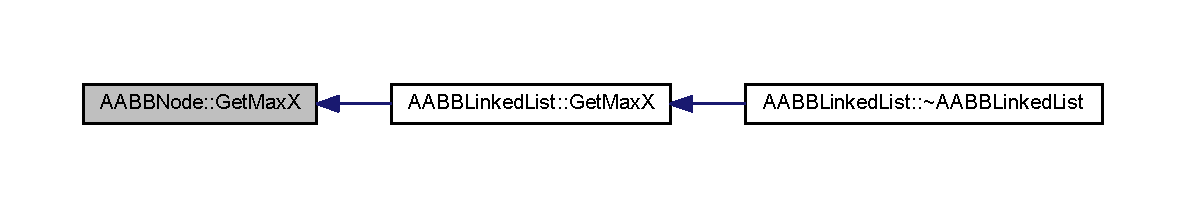
\includegraphics[width=350pt]{class_a_a_b_b_node_adb707da6d39fdae8230dd40f33a6cc85_icgraph}
\end{center}
\end{figure}


\index{A\+A\+B\+B\+Node@{A\+A\+B\+B\+Node}!Get\+MaxY@{Get\+MaxY}}
\index{Get\+MaxY@{Get\+MaxY}!A\+A\+B\+B\+Node@{A\+A\+B\+B\+Node}}
\subsubsection[{\texorpdfstring{Get\+Max\+Y()}{GetMaxY()}}]{\setlength{\rightskip}{0pt plus 5cm}G\+Ldouble A\+A\+B\+B\+Node\+::\+Get\+MaxY (
\begin{DoxyParamCaption}
{}
\end{DoxyParamCaption}
)\hspace{0.3cm}{\ttfamily [inline]}}\hypertarget{class_a_a_b_b_node_aca46418ff41fbadd321474617abe81e8}{}\label{class_a_a_b_b_node_aca46418ff41fbadd321474617abe81e8}


Here is the caller graph for this function\+:
\nopagebreak
\begin{figure}[H]
\begin{center}
\leavevmode
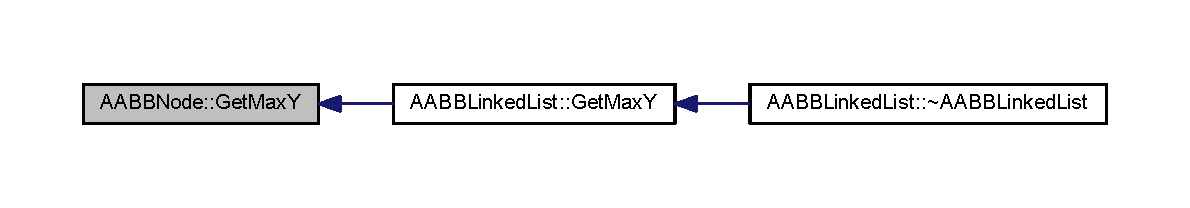
\includegraphics[width=350pt]{class_a_a_b_b_node_aca46418ff41fbadd321474617abe81e8_icgraph}
\end{center}
\end{figure}


\index{A\+A\+B\+B\+Node@{A\+A\+B\+B\+Node}!Get\+MaxZ@{Get\+MaxZ}}
\index{Get\+MaxZ@{Get\+MaxZ}!A\+A\+B\+B\+Node@{A\+A\+B\+B\+Node}}
\subsubsection[{\texorpdfstring{Get\+Max\+Z()}{GetMaxZ()}}]{\setlength{\rightskip}{0pt plus 5cm}G\+Ldouble A\+A\+B\+B\+Node\+::\+Get\+MaxZ (
\begin{DoxyParamCaption}
{}
\end{DoxyParamCaption}
)\hspace{0.3cm}{\ttfamily [inline]}}\hypertarget{class_a_a_b_b_node_a86f9e03ef5e39913c520b00dd06541e6}{}\label{class_a_a_b_b_node_a86f9e03ef5e39913c520b00dd06541e6}


Here is the caller graph for this function\+:
\nopagebreak
\begin{figure}[H]
\begin{center}
\leavevmode
\includegraphics[width=350pt]{class_a_a_b_b_node_a86f9e03ef5e39913c520b00dd06541e6_icgraph}
\end{center}
\end{figure}


\index{A\+A\+B\+B\+Node@{A\+A\+B\+B\+Node}!Get\+MinX@{Get\+MinX}}
\index{Get\+MinX@{Get\+MinX}!A\+A\+B\+B\+Node@{A\+A\+B\+B\+Node}}
\subsubsection[{\texorpdfstring{Get\+Min\+X()}{GetMinX()}}]{\setlength{\rightskip}{0pt plus 5cm}G\+Ldouble A\+A\+B\+B\+Node\+::\+Get\+MinX (
\begin{DoxyParamCaption}
{}
\end{DoxyParamCaption}
)\hspace{0.3cm}{\ttfamily [inline]}}\hypertarget{class_a_a_b_b_node_ada7009629434897aefb2b58384ae91e2}{}\label{class_a_a_b_b_node_ada7009629434897aefb2b58384ae91e2}


Here is the caller graph for this function\+:
\nopagebreak
\begin{figure}[H]
\begin{center}
\leavevmode
\includegraphics[width=350pt]{class_a_a_b_b_node_ada7009629434897aefb2b58384ae91e2_icgraph}
\end{center}
\end{figure}


\index{A\+A\+B\+B\+Node@{A\+A\+B\+B\+Node}!Get\+MinY@{Get\+MinY}}
\index{Get\+MinY@{Get\+MinY}!A\+A\+B\+B\+Node@{A\+A\+B\+B\+Node}}
\subsubsection[{\texorpdfstring{Get\+Min\+Y()}{GetMinY()}}]{\setlength{\rightskip}{0pt plus 5cm}G\+Ldouble A\+A\+B\+B\+Node\+::\+Get\+MinY (
\begin{DoxyParamCaption}
{}
\end{DoxyParamCaption}
)\hspace{0.3cm}{\ttfamily [inline]}}\hypertarget{class_a_a_b_b_node_a1dfa67f00ed2e48487df020eb5a20fd0}{}\label{class_a_a_b_b_node_a1dfa67f00ed2e48487df020eb5a20fd0}


Here is the caller graph for this function\+:
\nopagebreak
\begin{figure}[H]
\begin{center}
\leavevmode
\includegraphics[width=350pt]{class_a_a_b_b_node_a1dfa67f00ed2e48487df020eb5a20fd0_icgraph}
\end{center}
\end{figure}


\index{A\+A\+B\+B\+Node@{A\+A\+B\+B\+Node}!Get\+MinZ@{Get\+MinZ}}
\index{Get\+MinZ@{Get\+MinZ}!A\+A\+B\+B\+Node@{A\+A\+B\+B\+Node}}
\subsubsection[{\texorpdfstring{Get\+Min\+Z()}{GetMinZ()}}]{\setlength{\rightskip}{0pt plus 5cm}G\+Ldouble A\+A\+B\+B\+Node\+::\+Get\+MinZ (
\begin{DoxyParamCaption}
{}
\end{DoxyParamCaption}
)\hspace{0.3cm}{\ttfamily [inline]}}\hypertarget{class_a_a_b_b_node_a9d8ab82f585a852cc45cb1d8b27188cf}{}\label{class_a_a_b_b_node_a9d8ab82f585a852cc45cb1d8b27188cf}


Here is the caller graph for this function\+:
\nopagebreak
\begin{figure}[H]
\begin{center}
\leavevmode
\includegraphics[width=350pt]{class_a_a_b_b_node_a9d8ab82f585a852cc45cb1d8b27188cf_icgraph}
\end{center}
\end{figure}


\index{A\+A\+B\+B\+Node@{A\+A\+B\+B\+Node}!Get\+Next@{Get\+Next}}
\index{Get\+Next@{Get\+Next}!A\+A\+B\+B\+Node@{A\+A\+B\+B\+Node}}
\subsubsection[{\texorpdfstring{Get\+Next() const }{GetNext() const }}]{\setlength{\rightskip}{0pt plus 5cm}{\bf A\+A\+B\+B\+Node}$\ast$ A\+A\+B\+B\+Node\+::\+Get\+Next (
\begin{DoxyParamCaption}
{}
\end{DoxyParamCaption}
) const\hspace{0.3cm}{\ttfamily [inline]}}\hypertarget{class_a_a_b_b_node_aeba066c64653e3a9d73e0b617a8b844c}{}\label{class_a_a_b_b_node_aeba066c64653e3a9d73e0b617a8b844c}


Here is the call graph for this function\+:
\nopagebreak
\begin{figure}[H]
\begin{center}
\leavevmode
\includegraphics[width=331pt]{class_a_a_b_b_node_aeba066c64653e3a9d73e0b617a8b844c_cgraph}
\end{center}
\end{figure}




Here is the caller graph for this function\+:
\nopagebreak
\begin{figure}[H]
\begin{center}
\leavevmode
\includegraphics[width=350pt]{class_a_a_b_b_node_aeba066c64653e3a9d73e0b617a8b844c_icgraph}
\end{center}
\end{figure}


\index{A\+A\+B\+B\+Node@{A\+A\+B\+B\+Node}!operator=@{operator=}}
\index{operator=@{operator=}!A\+A\+B\+B\+Node@{A\+A\+B\+B\+Node}}
\subsubsection[{\texorpdfstring{operator=(const A\+A\+B\+B\+Node \&new\+Node)}{operator=(const AABBNode &newNode)}}]{\setlength{\rightskip}{0pt plus 5cm}{\bf A\+A\+B\+B\+Node}\& A\+A\+B\+B\+Node\+::operator= (
\begin{DoxyParamCaption}
\item[{const {\bf A\+A\+B\+B\+Node} \&}]{new\+Node}
\end{DoxyParamCaption}
)\hspace{0.3cm}{\ttfamily [inline]}, {\ttfamily [private]}}\hypertarget{class_a_a_b_b_node_aa4302db47c66af98472bcf6f42c6ba65}{}\label{class_a_a_b_b_node_aa4302db47c66af98472bcf6f42c6ba65}
\index{A\+A\+B\+B\+Node@{A\+A\+B\+B\+Node}!Set\+Data@{Set\+Data}}
\index{Set\+Data@{Set\+Data}!A\+A\+B\+B\+Node@{A\+A\+B\+B\+Node}}
\subsubsection[{\texorpdfstring{Set\+Data(const G\+Ldouble max\+X, const G\+Ldouble min\+X, const G\+Ldouble max\+Y, const G\+Ldouble min\+Y, const G\+Ldouble max\+Z, const G\+Ldouble min\+Z)}{SetData(const GLdouble maxX, const GLdouble minX, const GLdouble maxY, const GLdouble minY, const GLdouble maxZ, const GLdouble minZ)}}]{\setlength{\rightskip}{0pt plus 5cm}void A\+A\+B\+B\+Node\+::\+Set\+Data (
\begin{DoxyParamCaption}
\item[{const G\+Ldouble}]{maxX, }
\item[{const G\+Ldouble}]{minX, }
\item[{const G\+Ldouble}]{maxY, }
\item[{const G\+Ldouble}]{minY, }
\item[{const G\+Ldouble}]{maxZ, }
\item[{const G\+Ldouble}]{minZ}
\end{DoxyParamCaption}
)}\hypertarget{class_a_a_b_b_node_a43c049985e68d0d7443dc7ba11c71979}{}\label{class_a_a_b_b_node_a43c049985e68d0d7443dc7ba11c71979}


Here is the caller graph for this function\+:
\nopagebreak
\begin{figure}[H]
\begin{center}
\leavevmode
\includegraphics[width=350pt]{class_a_a_b_b_node_a43c049985e68d0d7443dc7ba11c71979_icgraph}
\end{center}
\end{figure}


\index{A\+A\+B\+B\+Node@{A\+A\+B\+B\+Node}!Set\+Next@{Set\+Next}}
\index{Set\+Next@{Set\+Next}!A\+A\+B\+B\+Node@{A\+A\+B\+B\+Node}}
\subsubsection[{\texorpdfstring{Set\+Next(\+A\+A\+B\+B\+Node $\ast$next)}{SetNext(AABBNode *next)}}]{\setlength{\rightskip}{0pt plus 5cm}void A\+A\+B\+B\+Node\+::\+Set\+Next (
\begin{DoxyParamCaption}
\item[{{\bf A\+A\+B\+B\+Node} $\ast$}]{next}
\end{DoxyParamCaption}
)\hspace{0.3cm}{\ttfamily [inline]}}\hypertarget{class_a_a_b_b_node_a2d624ad9c1241156af7a4dd96cbcd40f}{}\label{class_a_a_b_b_node_a2d624ad9c1241156af7a4dd96cbcd40f}


Here is the caller graph for this function\+:
\nopagebreak
\begin{figure}[H]
\begin{center}
\leavevmode
\includegraphics[width=350pt]{class_a_a_b_b_node_a2d624ad9c1241156af7a4dd96cbcd40f_icgraph}
\end{center}
\end{figure}




\subsection{Member Data Documentation}
\index{A\+A\+B\+B\+Node@{A\+A\+B\+B\+Node}!m\+\_\+\+B\+Box@{m\+\_\+\+B\+Box}}
\index{m\+\_\+\+B\+Box@{m\+\_\+\+B\+Box}!A\+A\+B\+B\+Node@{A\+A\+B\+B\+Node}}
\subsubsection[{\texorpdfstring{m\+\_\+\+B\+Box}{m_BBox}}]{\setlength{\rightskip}{0pt plus 5cm}{\bf Bounding\+Box} A\+A\+B\+B\+Node\+::m\+\_\+\+B\+Box\hspace{0.3cm}{\ttfamily [private]}}\hypertarget{class_a_a_b_b_node_ac45482982e70ba3d40c2099b99db0663}{}\label{class_a_a_b_b_node_ac45482982e70ba3d40c2099b99db0663}
\index{A\+A\+B\+B\+Node@{A\+A\+B\+B\+Node}!m\+\_\+next@{m\+\_\+next}}
\index{m\+\_\+next@{m\+\_\+next}!A\+A\+B\+B\+Node@{A\+A\+B\+B\+Node}}
\subsubsection[{\texorpdfstring{m\+\_\+next}{m_next}}]{\setlength{\rightskip}{0pt plus 5cm}{\bf A\+A\+B\+B\+Node}$\ast$ A\+A\+B\+B\+Node\+::m\+\_\+next\hspace{0.3cm}{\ttfamily [private]}}\hypertarget{class_a_a_b_b_node_a2fe0e4624db458571d0935f4b09ec415}{}\label{class_a_a_b_b_node_a2fe0e4624db458571d0935f4b09ec415}


The documentation for this class was generated from the following files\+:\begin{DoxyCompactItemize}
\item 
C\+:/000\+Uniwork/\+I\+C\+T290 Games Programming Try 2/\+Exercise 1/\+C\+A\+M\+P\+U\+S T\+O\+U\+R/\hyperlink{_a_a_b_b_node_8h}{A\+A\+B\+B\+Node.\+h}\item 
C\+:/000\+Uniwork/\+I\+C\+T290 Games Programming Try 2/\+Exercise 1/\+C\+A\+M\+P\+U\+S T\+O\+U\+R/\hyperlink{_a_a_b_b_node_8cpp}{A\+A\+B\+B\+Node.\+cpp}\end{DoxyCompactItemize}

\hypertarget{struct_a_a_b_b_1_1_bounding_box}{}\section{A\+A\+BB\+:\+:Bounding\+Box Struct Reference}
\label{struct_a_a_b_b_1_1_bounding_box}\index{A\+A\+B\+B\+::\+Bounding\+Box@{A\+A\+B\+B\+::\+Bounding\+Box}}


Collaboration diagram for A\+A\+BB\+:\+:Bounding\+Box\+:
\nopagebreak
\begin{figure}[H]
\begin{center}
\leavevmode
\includegraphics[width=187pt]{struct_a_a_b_b_1_1_bounding_box__coll__graph}
\end{center}
\end{figure}
\subsection*{Public Attributes}
\begin{DoxyCompactItemize}
\item 
\hyperlink{struct_a_a_b_b_1_1_x_y_z}{X\+YZ} \hyperlink{struct_a_a_b_b_1_1_bounding_box_a3eab345c474818852c6fc60fa78b9dd4}{max}
\item 
\hyperlink{struct_a_a_b_b_1_1_x_y_z}{X\+YZ} \hyperlink{struct_a_a_b_b_1_1_bounding_box_a47ffd944b2b41d2ebd1fee2f6d16a6d4}{min}
\end{DoxyCompactItemize}


\subsection{Member Data Documentation}
\index{A\+A\+B\+B\+::\+Bounding\+Box@{A\+A\+B\+B\+::\+Bounding\+Box}!max@{max}}
\index{max@{max}!A\+A\+B\+B\+::\+Bounding\+Box@{A\+A\+B\+B\+::\+Bounding\+Box}}
\subsubsection[{\texorpdfstring{max}{max}}]{\setlength{\rightskip}{0pt plus 5cm}{\bf X\+YZ} A\+A\+B\+B\+::\+Bounding\+Box\+::max}\hypertarget{struct_a_a_b_b_1_1_bounding_box_a3eab345c474818852c6fc60fa78b9dd4}{}\label{struct_a_a_b_b_1_1_bounding_box_a3eab345c474818852c6fc60fa78b9dd4}
\index{A\+A\+B\+B\+::\+Bounding\+Box@{A\+A\+B\+B\+::\+Bounding\+Box}!min@{min}}
\index{min@{min}!A\+A\+B\+B\+::\+Bounding\+Box@{A\+A\+B\+B\+::\+Bounding\+Box}}
\subsubsection[{\texorpdfstring{min}{min}}]{\setlength{\rightskip}{0pt plus 5cm}{\bf X\+YZ} A\+A\+B\+B\+::\+Bounding\+Box\+::min}\hypertarget{struct_a_a_b_b_1_1_bounding_box_a47ffd944b2b41d2ebd1fee2f6d16a6d4}{}\label{struct_a_a_b_b_1_1_bounding_box_a47ffd944b2b41d2ebd1fee2f6d16a6d4}


The documentation for this struct was generated from the following file\+:\begin{DoxyCompactItemize}
\item 
C\+:/000\+Uniwork/\+I\+C\+T290 Games Programming Try 2/\+Exercise 1/\+C\+A\+M\+P\+U\+S T\+O\+U\+R/\hyperlink{_a_a_b_b_8_h}{A\+A\+B\+B.\+H}\end{DoxyCompactItemize}

\hypertarget{struct_a_a_b_b_node_1_1_bounding_box}{}\section{A\+A\+B\+B\+Node\+:\+:Bounding\+Box Struct Reference}
\label{struct_a_a_b_b_node_1_1_bounding_box}\index{A\+A\+B\+B\+Node\+::\+Bounding\+Box@{A\+A\+B\+B\+Node\+::\+Bounding\+Box}}


Collaboration diagram for A\+A\+B\+B\+Node\+:\+:Bounding\+Box\+:
\nopagebreak
\begin{figure}[H]
\begin{center}
\leavevmode
\includegraphics[width=210pt]{struct_a_a_b_b_node_1_1_bounding_box__coll__graph}
\end{center}
\end{figure}
\subsection*{Public Attributes}
\begin{DoxyCompactItemize}
\item 
\hyperlink{struct_a_a_b_b_node_1_1_x_y_z}{X\+YZ} \hyperlink{struct_a_a_b_b_node_1_1_bounding_box_a75e2a4b821ffd9327092d1911fba647a}{max}
\item 
\hyperlink{struct_a_a_b_b_node_1_1_x_y_z}{X\+YZ} \hyperlink{struct_a_a_b_b_node_1_1_bounding_box_a9c046f23dd984b1bc04afe0257b68657}{min}
\end{DoxyCompactItemize}


\subsection{Member Data Documentation}
\index{A\+A\+B\+B\+Node\+::\+Bounding\+Box@{A\+A\+B\+B\+Node\+::\+Bounding\+Box}!max@{max}}
\index{max@{max}!A\+A\+B\+B\+Node\+::\+Bounding\+Box@{A\+A\+B\+B\+Node\+::\+Bounding\+Box}}
\subsubsection[{\texorpdfstring{max}{max}}]{\setlength{\rightskip}{0pt plus 5cm}{\bf X\+YZ} A\+A\+B\+B\+Node\+::\+Bounding\+Box\+::max}\hypertarget{struct_a_a_b_b_node_1_1_bounding_box_a75e2a4b821ffd9327092d1911fba647a}{}\label{struct_a_a_b_b_node_1_1_bounding_box_a75e2a4b821ffd9327092d1911fba647a}
\index{A\+A\+B\+B\+Node\+::\+Bounding\+Box@{A\+A\+B\+B\+Node\+::\+Bounding\+Box}!min@{min}}
\index{min@{min}!A\+A\+B\+B\+Node\+::\+Bounding\+Box@{A\+A\+B\+B\+Node\+::\+Bounding\+Box}}
\subsubsection[{\texorpdfstring{min}{min}}]{\setlength{\rightskip}{0pt plus 5cm}{\bf X\+YZ} A\+A\+B\+B\+Node\+::\+Bounding\+Box\+::min}\hypertarget{struct_a_a_b_b_node_1_1_bounding_box_a9c046f23dd984b1bc04afe0257b68657}{}\label{struct_a_a_b_b_node_1_1_bounding_box_a9c046f23dd984b1bc04afe0257b68657}


The documentation for this struct was generated from the following file\+:\begin{DoxyCompactItemize}
\item 
C\+:/000\+Uniwork/\+I\+C\+T290 Games Programming Try 2/\+Exercise 1/\+C\+A\+M\+P\+U\+S T\+O\+U\+R/\hyperlink{_a_a_b_b_node_8h}{A\+A\+B\+B\+Node.\+h}\end{DoxyCompactItemize}

\hypertarget{class_camera}{}\section{Camera Class Reference}
\label{class_camera}\index{Camera@{Camera}}


{\ttfamily \#include $<$camera.\+h$>$}



Collaboration diagram for Camera\+:
\nopagebreak
\begin{figure}[H]
\begin{center}
\leavevmode
\includegraphics[width=350pt]{class_camera__coll__graph}
\end{center}
\end{figure}
\subsection*{Public Member Functions}
\begin{DoxyCompactItemize}
\item 
\hyperlink{class_camera_a01f94c3543f56ede7af49dc778f19331}{Camera} ()
\item 
virtual \hyperlink{class_camera_ac9ed2a1433c5afdfb9cdf5b282fbc350}{$\sim$\+Camera} ()
\item 
void \hyperlink{class_camera_a57b68a39284d0c249676a3dba70bac05}{Set\+A\+A\+B\+B\+MaxX} (const int \&temp\+Index, const G\+Ldouble \&tempX)
\item 
void \hyperlink{class_camera_a4c0c8094ebcf2c5255e064ebbb7d562c}{Set\+A\+A\+B\+B\+MinX} (const int \&temp\+Index, const G\+Ldouble \&tempX)
\item 
void \hyperlink{class_camera_a5645577a695fb4b5b59aa948882a27d4}{Set\+A\+A\+B\+B\+MaxY} (const int \&temp\+Index, const G\+Ldouble \&tempY)
\item 
void \hyperlink{class_camera_aa3b852f1208a5e2c9bfa0ee6d1c8e8cc}{Set\+A\+A\+B\+B\+MinY} (const int \&temp\+Index, const G\+Ldouble \&tempY)
\item 
void \hyperlink{class_camera_aaf211279f0439d31fa1d885f1a630db9}{Set\+A\+A\+B\+B\+MaxZ} (const int \&temp\+Index, const G\+Ldouble \&tempZ)
\item 
void \hyperlink{class_camera_ae5dfebfe1c8a018fb2ce96803b6f2c49}{Set\+A\+A\+B\+B\+MinZ} (const int \&temp\+Index, const G\+Ldouble \&tempZ)
\item 
void \hyperlink{class_camera_af1b56a7aee4d2b0c38054e05c0553e51}{Set\+Rotate\+Speed} (const G\+Ldouble \&temp\+Speed)
\item 
void \hyperlink{class_camera_a86a5a6f374125bb58c6a97ba2d921a64}{Set\+Move\+Speed} (const G\+Ldouble \&temp\+Speed)
\item 
void \hyperlink{class_camera_a63b20dd514c4e3fc9990d6a61151387c}{Set\+Collision\+Detection\+On} (const bool \&temp\+Col)
\item 
void \hyperlink{class_camera_a043549232a16c18fe93f35c5d3a40fe2}{Set\+No\+Bounding\+Boxes} (const int \&temp\+Size)
\item 
void \hyperlink{class_camera_a32f72b80b7aaf7a1623dc68239bd446b}{Set\+World\+Coordinates} (const G\+Ldouble \&tempX, const G\+Ldouble \&tempZ)
\item 
void \hyperlink{class_camera_af39ed792820436b916a4d6110413423f}{Initiate\+Bounding\+Boxes} ()
\item 
void \hyperlink{class_camera_a5b5c1468bdb3b8e6e654bea66c9561b8}{Set\+Plains} (const int temp\+Type, const G\+Ldouble temp\+Xs, const G\+Ldouble temp\+Xe, const G\+Ldouble temp\+Ys, const G\+Ldouble temp\+Ye, const G\+Ldouble temp\+Zs, const G\+Ldouble temp\+Ze)
\item 
G\+Ldouble \hyperlink{class_camera_a5d71756678367cc9ef6d3186dff7e821}{Get\+LR} ()
\item 
G\+Ldouble \hyperlink{class_camera_acaa842acd09e3a18c409ddc0c89cf808}{Get\+UD} ()
\item 
G\+Ldouble \hyperlink{class_camera_a2c82b9713e7cc1fb77130aad72728478}{Get\+FB} ()
\item 
G\+Ldouble \hyperlink{class_camera_a60cc1df56165f876367b82bf3016879d}{Get\+A\+A\+B\+B\+MaxX} (const int \&temp\+Index)
\item 
G\+Ldouble \hyperlink{class_camera_a7b0c8231ff696a81330b0960ee4ff719}{Get\+A\+A\+B\+B\+MinX} (const int \&temp\+Index)
\item 
G\+Ldouble \hyperlink{class_camera_a65002f8d31f7d541284126550e033c12}{Get\+A\+A\+B\+B\+MaxY} (const int \&temp\+Index)
\item 
G\+Ldouble \hyperlink{class_camera_adcd706fee322ada843a3ac753aa69549}{Get\+A\+A\+B\+B\+MinY} (const int \&temp\+Index)
\item 
G\+Ldouble \hyperlink{class_camera_a8cba314f46549c3d71be172b86ad5fe0}{Get\+A\+A\+B\+B\+MaxZ} (const int \&temp\+Index)
\item 
G\+Ldouble \hyperlink{class_camera_a333f233675f83907a0f8a8e3274865fe}{Get\+A\+A\+B\+B\+MinZ} (const int \&temp\+Index)
\item 
void \hyperlink{class_camera_a259204729f7a60277c6f6215559adcc0}{Position} (G\+Ldouble const \&tempX, G\+Ldouble const \&tempY, G\+Ldouble const \&tempZ, G\+Ldouble const \&temp\+Angle)
\item 
void \hyperlink{class_camera_a5757577b0e11b8722bf251ee086eef1d}{Check\+Camera} ()
\item 
void \hyperlink{class_camera_a19d7bf6f171a46abe5b7743c0429ca75}{Direction\+FB} (int const \&temp\+Move)
\item 
void \hyperlink{class_camera_a11f6493139834cc9d31a1c28e5effa1a}{Direction\+LR} (int const \&temp\+Move)
\item 
void \hyperlink{class_camera_a3134cb509a1167898806c94bf6f3bf28}{Direction\+UD} (int const \&temp\+Move)
\item 
void \hyperlink{class_camera_a9b7f4a96faa388248f8350c733789688}{Direction\+Rotate\+LR} (G\+Ldouble const \&temp\+Move)
\item 
void \hyperlink{class_camera_a7271df5741bcbe72f464729f8d80ad43}{Direction\+Look\+UD} (int const \&temp\+Move)
\item 
void \hyperlink{class_camera_adc12edf020e48254432214200f8e63c3}{Display\+Map} (const int \&screen\+Width, const int \&screen\+Height, const G\+Luint \&temp\+Image)
\item 
void \hyperlink{class_camera_ab8084e679b9cf9bf9a6e333ca8a0caee}{Display\+Welcome\+Screen} (const int \&screen\+Width, const int \&screen\+Height, const int \&temp\+Exit, const G\+Luint \&temp\+Image)
\item 
void \hyperlink{class_camera_a182d23d247e640ba1ed267332a8a6dd0}{Display\+No\+Exit} (const int \&screen\+Width, const int \&screen\+Height, const G\+Luint \&temp\+Image)
\end{DoxyCompactItemize}
\subsection*{Private Member Functions}
\begin{DoxyCompactItemize}
\item 
bool \hyperlink{class_camera_a8937b6b035801d1f698b40693c53d1e6}{Move\+F\+B\+OK} ()
\item 
bool \hyperlink{class_camera_a4e500f9773f9f46a69e6a70d40d838bf}{Move\+L\+R\+OK} ()
\item 
bool \hyperlink{class_camera_a3bb636079c02cdb8ac235c157faa4556}{Move\+U\+D\+OK} ()
\item 
bool \hyperlink{class_camera_a5c352dbad24a210bf0159e00f1dfe8b8}{Rotate\+L\+R\+OK} ()
\item 
bool \hyperlink{class_camera_a3b3f5cedfa0d89824ea52f109bc3eba8}{Look\+U\+D\+OK} ()
\item 
void \hyperlink{class_camera_acc808e653e9c59f0d2450c9caca26b98}{Move\+FB} ()
\item 
void \hyperlink{class_camera_ad53c2248f2d38bc8f01ac288e8cc21d3}{Move\+LR} ()
\item 
void \hyperlink{class_camera_af14abc814d362ed9781db6725919f836}{Move\+UD} ()
\item 
void \hyperlink{class_camera_aff5a71068d0d6f82c5a03efe1c9be259}{Rotate\+LR} ()
\item 
void \hyperlink{class_camera_ae72895a4f32cdc88146bee6a1a3ea636}{Look\+UD} ()
\item 
void \hyperlink{class_camera_a62b9c31a39202f116f3b9fd774ef42e3}{Set\+Plains} (const int \&moveX, const int \&moveZ)
\item 
void \hyperlink{class_camera_a11d15ac81e6fbe74c1dd09e342be3e9c}{Reset\+X\+YZ} ()
\item 
void \hyperlink{class_camera_a023cb3e9d92301d8132f338c7ef5be77}{call\+G\+L\+Look\+At} ()
\item 
void \hyperlink{class_camera_ae1798d33c0a7379dc227cc18dc767732}{Climb\+Steps} (G\+Ldouble step\+Start, G\+Ldouble step\+Finish, G\+Ldouble step\+Height, G\+Ldouble step\+Width, int no\+Steps)
\item 
void \hyperlink{class_camera_aedb7c813456b1856f098a8733d7f4e1b}{Check\+Steps} ()
\item 
\hyperlink{class_camera_ac01065de99da2319fb5fd4fc1ba96ea3}{Camera} (const \hyperlink{class_camera}{Camera} \&\hyperlink{main_8cpp_a3b23650c3f80b53cee3a2c471797c732}{cam})
\item 
\hyperlink{class_camera}{Camera} \& \hyperlink{class_camera_a5a6ef1328b993f207ab51755e7d19341}{operator=} (const \hyperlink{class_camera}{Camera} \&\hyperlink{main_8cpp_a3b23650c3f80b53cee3a2c471797c732}{cam})
\end{DoxyCompactItemize}
\subsection*{Private Attributes}
\begin{DoxyCompactItemize}
\item 
G\+Ldouble \hyperlink{class_camera_ac25bd676d0c76ec08ab47c2c12d553e6}{m\+\_\+incrementX}
\item 
G\+Ldouble \hyperlink{class_camera_a777eebd5eecb1611eee536cfa5f31352}{m\+\_\+incrementZ}
\item 
int \hyperlink{class_camera_a0f0d872791aed39f2ac08f402f647915}{m\+\_\+\+No\+\_\+\+Plains}
\item 
int \hyperlink{class_camera_ac5693b74a6d1e8dfd24e0166166b5945}{m\+\_\+plain\+No}
\item 
G\+Ldouble \hyperlink{class_camera_ac7817dd04945678fc56b9384d85aeb5a}{m\+\_\+plain\+Height}
\item 
G\+Ldouble \hyperlink{class_camera_a2cec5d8ebb2cf924f341f2c8380dd3b0}{m\+\_\+rotate\+Angle\+LR}
\item 
G\+Ldouble \hyperlink{class_camera_aaee679a1afd9606b73b3aced250b6cc8}{m\+\_\+delta\+Angle\+LR}
\item 
G\+Ldouble \hyperlink{class_camera_a732416affaf942ce888b09c4ebf21d1c}{m\+\_\+rotate\+Angle\+UD}
\item 
G\+Ldouble \hyperlink{class_camera_aa7b595dcc6baf3ad640fddf4c5324255}{m\+\_\+delta\+Angle\+UD}
\item 
G\+Ldouble \hyperlink{class_camera_a25bb32ac42de7c4dd7363346e67f5109}{m\+\_\+x}
\item 
G\+Ldouble \hyperlink{class_camera_a453ac6c0c996ba47cc1783d45566a893}{m\+\_\+y}
\item 
G\+Ldouble \hyperlink{class_camera_a34fa5e648d04f0648e397ea7bde2d717}{m\+\_\+z}
\item 
G\+Ldouble \hyperlink{class_camera_ae08110e1bfe81d6f019924c0e67f3373}{m\+\_\+z\+Last}
\item 
G\+Ldouble \hyperlink{class_camera_ae5fb587e1a44ba40f7978e4425480192}{m\+\_\+x\+Last}
\item 
G\+Ldouble \hyperlink{class_camera_ab7ffaf41adca8d8d233cc7317ffff47b}{m\+\_\+lookX}
\item 
G\+Ldouble \hyperlink{class_camera_a319433486f0d49d9a0689d92ff7a9c71}{m\+\_\+lookY}
\item 
G\+Ldouble \hyperlink{class_camera_a8c78671164cc57c2e543e72dbd45f0e5}{m\+\_\+lookZ}
\item 
G\+Ldouble \hyperlink{class_camera_a911721fe8284d96a8b39f2643697f9b8}{m\+\_\+look\+XX}
\item 
G\+Ldouble \hyperlink{class_camera_aa3dec6999681086ca8554ae1064ea981}{m\+\_\+look\+YY}
\item 
G\+Ldouble \hyperlink{class_camera_a56ed44a9568055cdd08ea722f9cc6ec2}{m\+\_\+look\+ZZ}
\item 
G\+Ldouble \hyperlink{class_camera_a926b86f367bdc0cae1783498b39ae4cd}{m\+\_\+delta\+Move\+LR}
\item 
G\+Ldouble \hyperlink{class_camera_a07005a18b67f5cedf2da83fecf419be1}{m\+\_\+delta\+Move\+FB}
\item 
G\+Ldouble \hyperlink{class_camera_acff5854969204b936ffa3f725978a9e0}{m\+\_\+delta\+Move\+UD}
\item 
G\+Ldouble \hyperlink{class_camera_a1effa9e036ee79639576c98309b3167c}{m\+\_\+direction}
\item 
G\+Ldouble \hyperlink{class_camera_a6bb4538eac6b62a28b54d44bf29fa43e}{m\+\_\+rotate\+Speed}
\item 
G\+Ldouble \hyperlink{class_camera_ac3af0da038084aef9d6fe40034c5ca32}{m\+\_\+move\+Speed}
\item 
bool \hyperlink{class_camera_a05187d2d2ade85f02b9b64f3609be183}{m\+\_\+\+Collision\+Detection\+On}
\item 
\hyperlink{class_collision}{Collision} \hyperlink{class_camera_a1e22adb9c7075912a96bae63b6e207eb}{m\+\_\+col\+Detect}
\item 
\hyperlink{class_camera_map}{Camera\+Map} \hyperlink{class_camera_adb7e6447abcabd554a16aee09a7e1fbd}{m\+\_\+map}
\item 
\hyperlink{class_plain_linked_list}{Plain\+Linked\+List} \hyperlink{class_camera_aea1d08ac0b682512dcd09ba37ef3fc78}{m\+\_\+\+Plain}
\item 
\hyperlink{class_c_easy_sound}{C\+Easy\+Sound} $\ast$ \hyperlink{class_camera_a3972ee2951a400a843420cb81ade3e86}{es}
\item 
\hyperlink{class_c_sound}{C\+Sound} $\ast$ \hyperlink{class_camera_af49515a2c895ccb07b3a7ba8644b9cc3}{step\+Sound}
\end{DoxyCompactItemize}


\subsection{Constructor \& Destructor Documentation}
\index{Camera@{Camera}!Camera@{Camera}}
\index{Camera@{Camera}!Camera@{Camera}}
\subsubsection[{\texorpdfstring{Camera()}{Camera()}}]{\setlength{\rightskip}{0pt plus 5cm}Camera\+::\+Camera (
\begin{DoxyParamCaption}
{}
\end{DoxyParamCaption}
)}\hypertarget{class_camera_a01f94c3543f56ede7af49dc778f19331}{}\label{class_camera_a01f94c3543f56ede7af49dc778f19331}


Here is the call graph for this function\+:
\nopagebreak
\begin{figure}[H]
\begin{center}
\leavevmode
\includegraphics[width=350pt]{class_camera_a01f94c3543f56ede7af49dc778f19331_cgraph}
\end{center}
\end{figure}


\index{Camera@{Camera}!````~Camera@{$\sim$\+Camera}}
\index{````~Camera@{$\sim$\+Camera}!Camera@{Camera}}
\subsubsection[{\texorpdfstring{$\sim$\+Camera()}{~Camera()}}]{\setlength{\rightskip}{0pt plus 5cm}virtual Camera\+::$\sim$\+Camera (
\begin{DoxyParamCaption}
{}
\end{DoxyParamCaption}
)\hspace{0.3cm}{\ttfamily [inline]}, {\ttfamily [virtual]}}\hypertarget{class_camera_ac9ed2a1433c5afdfb9cdf5b282fbc350}{}\label{class_camera_ac9ed2a1433c5afdfb9cdf5b282fbc350}


Here is the call graph for this function\+:
\nopagebreak
\begin{figure}[H]
\begin{center}
\leavevmode
\includegraphics[width=322pt]{class_camera_ac9ed2a1433c5afdfb9cdf5b282fbc350_cgraph}
\end{center}
\end{figure}


\index{Camera@{Camera}!Camera@{Camera}}
\index{Camera@{Camera}!Camera@{Camera}}
\subsubsection[{\texorpdfstring{Camera(const Camera \&cam)}{Camera(const Camera &cam)}}]{\setlength{\rightskip}{0pt plus 5cm}Camera\+::\+Camera (
\begin{DoxyParamCaption}
\item[{const {\bf Camera} \&}]{cam}
\end{DoxyParamCaption}
)\hspace{0.3cm}{\ttfamily [inline]}, {\ttfamily [private]}}\hypertarget{class_camera_ac01065de99da2319fb5fd4fc1ba96ea3}{}\label{class_camera_ac01065de99da2319fb5fd4fc1ba96ea3}


\subsection{Member Function Documentation}
\index{Camera@{Camera}!call\+G\+L\+Look\+At@{call\+G\+L\+Look\+At}}
\index{call\+G\+L\+Look\+At@{call\+G\+L\+Look\+At}!Camera@{Camera}}
\subsubsection[{\texorpdfstring{call\+G\+L\+Look\+At()}{callGLLookAt()}}]{\setlength{\rightskip}{0pt plus 5cm}void Camera\+::call\+G\+L\+Look\+At (
\begin{DoxyParamCaption}
{}
\end{DoxyParamCaption}
)\hspace{0.3cm}{\ttfamily [private]}}\hypertarget{class_camera_a023cb3e9d92301d8132f338c7ef5be77}{}\label{class_camera_a023cb3e9d92301d8132f338c7ef5be77}


Here is the caller graph for this function\+:
\nopagebreak
\begin{figure}[H]
\begin{center}
\leavevmode
\includegraphics[width=350pt]{class_camera_a023cb3e9d92301d8132f338c7ef5be77_icgraph}
\end{center}
\end{figure}


\index{Camera@{Camera}!Check\+Camera@{Check\+Camera}}
\index{Check\+Camera@{Check\+Camera}!Camera@{Camera}}
\subsubsection[{\texorpdfstring{Check\+Camera()}{CheckCamera()}}]{\setlength{\rightskip}{0pt plus 5cm}void Camera\+::\+Check\+Camera (
\begin{DoxyParamCaption}
{}
\end{DoxyParamCaption}
)}\hypertarget{class_camera_a5757577b0e11b8722bf251ee086eef1d}{}\label{class_camera_a5757577b0e11b8722bf251ee086eef1d}


Here is the call graph for this function\+:
\nopagebreak
\begin{figure}[H]
\begin{center}
\leavevmode
\includegraphics[width=350pt]{class_camera_a5757577b0e11b8722bf251ee086eef1d_cgraph}
\end{center}
\end{figure}




Here is the caller graph for this function\+:
\nopagebreak
\begin{figure}[H]
\begin{center}
\leavevmode
\includegraphics[width=350pt]{class_camera_a5757577b0e11b8722bf251ee086eef1d_icgraph}
\end{center}
\end{figure}


\index{Camera@{Camera}!Check\+Steps@{Check\+Steps}}
\index{Check\+Steps@{Check\+Steps}!Camera@{Camera}}
\subsubsection[{\texorpdfstring{Check\+Steps()}{CheckSteps()}}]{\setlength{\rightskip}{0pt plus 5cm}void Camera\+::\+Check\+Steps (
\begin{DoxyParamCaption}
{}
\end{DoxyParamCaption}
)\hspace{0.3cm}{\ttfamily [private]}}\hypertarget{class_camera_aedb7c813456b1856f098a8733d7f4e1b}{}\label{class_camera_aedb7c813456b1856f098a8733d7f4e1b}
\index{Camera@{Camera}!Climb\+Steps@{Climb\+Steps}}
\index{Climb\+Steps@{Climb\+Steps}!Camera@{Camera}}
\subsubsection[{\texorpdfstring{Climb\+Steps(\+G\+Ldouble step\+Start, G\+Ldouble step\+Finish, G\+Ldouble step\+Height, G\+Ldouble step\+Width, int no\+Steps)}{ClimbSteps(GLdouble stepStart, GLdouble stepFinish, GLdouble stepHeight, GLdouble stepWidth, int noSteps)}}]{\setlength{\rightskip}{0pt plus 5cm}void Camera\+::\+Climb\+Steps (
\begin{DoxyParamCaption}
\item[{G\+Ldouble}]{step\+Start, }
\item[{G\+Ldouble}]{step\+Finish, }
\item[{G\+Ldouble}]{step\+Height, }
\item[{G\+Ldouble}]{step\+Width, }
\item[{int}]{no\+Steps}
\end{DoxyParamCaption}
)\hspace{0.3cm}{\ttfamily [private]}}\hypertarget{class_camera_ae1798d33c0a7379dc227cc18dc767732}{}\label{class_camera_ae1798d33c0a7379dc227cc18dc767732}


Here is the call graph for this function\+:
\nopagebreak
\begin{figure}[H]
\begin{center}
\leavevmode
\includegraphics[width=330pt]{class_camera_ae1798d33c0a7379dc227cc18dc767732_cgraph}
\end{center}
\end{figure}


\index{Camera@{Camera}!Direction\+FB@{Direction\+FB}}
\index{Direction\+FB@{Direction\+FB}!Camera@{Camera}}
\subsubsection[{\texorpdfstring{Direction\+F\+B(int const \&temp\+Move)}{DirectionFB(int const &tempMove)}}]{\setlength{\rightskip}{0pt plus 5cm}void Camera\+::\+Direction\+FB (
\begin{DoxyParamCaption}
\item[{int const \&}]{temp\+Move}
\end{DoxyParamCaption}
)}\hypertarget{class_camera_a19d7bf6f171a46abe5b7743c0429ca75}{}\label{class_camera_a19d7bf6f171a46abe5b7743c0429ca75}


Here is the caller graph for this function\+:
\nopagebreak
\begin{figure}[H]
\begin{center}
\leavevmode
\includegraphics[width=350pt]{class_camera_a19d7bf6f171a46abe5b7743c0429ca75_icgraph}
\end{center}
\end{figure}


\index{Camera@{Camera}!Direction\+Look\+UD@{Direction\+Look\+UD}}
\index{Direction\+Look\+UD@{Direction\+Look\+UD}!Camera@{Camera}}
\subsubsection[{\texorpdfstring{Direction\+Look\+U\+D(int const \&temp\+Move)}{DirectionLookUD(int const &tempMove)}}]{\setlength{\rightskip}{0pt plus 5cm}void Camera\+::\+Direction\+Look\+UD (
\begin{DoxyParamCaption}
\item[{int const \&}]{temp\+Move}
\end{DoxyParamCaption}
)}\hypertarget{class_camera_a7271df5741bcbe72f464729f8d80ad43}{}\label{class_camera_a7271df5741bcbe72f464729f8d80ad43}


Here is the caller graph for this function\+:
\nopagebreak
\begin{figure}[H]
\begin{center}
\leavevmode
\includegraphics[width=350pt]{class_camera_a7271df5741bcbe72f464729f8d80ad43_icgraph}
\end{center}
\end{figure}


\index{Camera@{Camera}!Direction\+LR@{Direction\+LR}}
\index{Direction\+LR@{Direction\+LR}!Camera@{Camera}}
\subsubsection[{\texorpdfstring{Direction\+L\+R(int const \&temp\+Move)}{DirectionLR(int const &tempMove)}}]{\setlength{\rightskip}{0pt plus 5cm}void Camera\+::\+Direction\+LR (
\begin{DoxyParamCaption}
\item[{int const \&}]{temp\+Move}
\end{DoxyParamCaption}
)}\hypertarget{class_camera_a11f6493139834cc9d31a1c28e5effa1a}{}\label{class_camera_a11f6493139834cc9d31a1c28e5effa1a}


Here is the caller graph for this function\+:
\nopagebreak
\begin{figure}[H]
\begin{center}
\leavevmode
\includegraphics[width=350pt]{class_camera_a11f6493139834cc9d31a1c28e5effa1a_icgraph}
\end{center}
\end{figure}


\index{Camera@{Camera}!Direction\+Rotate\+LR@{Direction\+Rotate\+LR}}
\index{Direction\+Rotate\+LR@{Direction\+Rotate\+LR}!Camera@{Camera}}
\subsubsection[{\texorpdfstring{Direction\+Rotate\+L\+R(\+G\+Ldouble const \&temp\+Move)}{DirectionRotateLR(GLdouble const &tempMove)}}]{\setlength{\rightskip}{0pt plus 5cm}void Camera\+::\+Direction\+Rotate\+LR (
\begin{DoxyParamCaption}
\item[{G\+Ldouble const \&}]{temp\+Move}
\end{DoxyParamCaption}
)}\hypertarget{class_camera_a9b7f4a96faa388248f8350c733789688}{}\label{class_camera_a9b7f4a96faa388248f8350c733789688}


Here is the caller graph for this function\+:
\nopagebreak
\begin{figure}[H]
\begin{center}
\leavevmode
\includegraphics[width=350pt]{class_camera_a9b7f4a96faa388248f8350c733789688_icgraph}
\end{center}
\end{figure}


\index{Camera@{Camera}!Direction\+UD@{Direction\+UD}}
\index{Direction\+UD@{Direction\+UD}!Camera@{Camera}}
\subsubsection[{\texorpdfstring{Direction\+U\+D(int const \&temp\+Move)}{DirectionUD(int const &tempMove)}}]{\setlength{\rightskip}{0pt plus 5cm}void Camera\+::\+Direction\+UD (
\begin{DoxyParamCaption}
\item[{int const \&}]{temp\+Move}
\end{DoxyParamCaption}
)}\hypertarget{class_camera_a3134cb509a1167898806c94bf6f3bf28}{}\label{class_camera_a3134cb509a1167898806c94bf6f3bf28}


Here is the caller graph for this function\+:
\nopagebreak
\begin{figure}[H]
\begin{center}
\leavevmode
\includegraphics[width=344pt]{class_camera_a3134cb509a1167898806c94bf6f3bf28_icgraph}
\end{center}
\end{figure}


\index{Camera@{Camera}!Display\+Map@{Display\+Map}}
\index{Display\+Map@{Display\+Map}!Camera@{Camera}}
\subsubsection[{\texorpdfstring{Display\+Map(const int \&screen\+Width, const int \&screen\+Height, const G\+Luint \&temp\+Image)}{DisplayMap(const int &screenWidth, const int &screenHeight, const GLuint &tempImage)}}]{\setlength{\rightskip}{0pt plus 5cm}void Camera\+::\+Display\+Map (
\begin{DoxyParamCaption}
\item[{const int \&}]{screen\+Width, }
\item[{const int \&}]{screen\+Height, }
\item[{const G\+Luint \&}]{temp\+Image}
\end{DoxyParamCaption}
)}\hypertarget{class_camera_adc12edf020e48254432214200f8e63c3}{}\label{class_camera_adc12edf020e48254432214200f8e63c3}


Here is the call graph for this function\+:
\nopagebreak
\begin{figure}[H]
\begin{center}
\leavevmode
\includegraphics[width=349pt]{class_camera_adc12edf020e48254432214200f8e63c3_cgraph}
\end{center}
\end{figure}




Here is the caller graph for this function\+:
\nopagebreak
\begin{figure}[H]
\begin{center}
\leavevmode
\includegraphics[width=350pt]{class_camera_adc12edf020e48254432214200f8e63c3_icgraph}
\end{center}
\end{figure}


\index{Camera@{Camera}!Display\+No\+Exit@{Display\+No\+Exit}}
\index{Display\+No\+Exit@{Display\+No\+Exit}!Camera@{Camera}}
\subsubsection[{\texorpdfstring{Display\+No\+Exit(const int \&screen\+Width, const int \&screen\+Height, const G\+Luint \&temp\+Image)}{DisplayNoExit(const int &screenWidth, const int &screenHeight, const GLuint &tempImage)}}]{\setlength{\rightskip}{0pt plus 5cm}void Camera\+::\+Display\+No\+Exit (
\begin{DoxyParamCaption}
\item[{const int \&}]{screen\+Width, }
\item[{const int \&}]{screen\+Height, }
\item[{const G\+Luint \&}]{temp\+Image}
\end{DoxyParamCaption}
)}\hypertarget{class_camera_a182d23d247e640ba1ed267332a8a6dd0}{}\label{class_camera_a182d23d247e640ba1ed267332a8a6dd0}


Here is the call graph for this function\+:
\nopagebreak
\begin{figure}[H]
\begin{center}
\leavevmode
\includegraphics[width=350pt]{class_camera_a182d23d247e640ba1ed267332a8a6dd0_cgraph}
\end{center}
\end{figure}




Here is the caller graph for this function\+:
\nopagebreak
\begin{figure}[H]
\begin{center}
\leavevmode
\includegraphics[width=350pt]{class_camera_a182d23d247e640ba1ed267332a8a6dd0_icgraph}
\end{center}
\end{figure}


\index{Camera@{Camera}!Display\+Welcome\+Screen@{Display\+Welcome\+Screen}}
\index{Display\+Welcome\+Screen@{Display\+Welcome\+Screen}!Camera@{Camera}}
\subsubsection[{\texorpdfstring{Display\+Welcome\+Screen(const int \&screen\+Width, const int \&screen\+Height, const int \&temp\+Exit, const G\+Luint \&temp\+Image)}{DisplayWelcomeScreen(const int &screenWidth, const int &screenHeight, const int &tempExit, const GLuint &tempImage)}}]{\setlength{\rightskip}{0pt plus 5cm}void Camera\+::\+Display\+Welcome\+Screen (
\begin{DoxyParamCaption}
\item[{const int \&}]{screen\+Width, }
\item[{const int \&}]{screen\+Height, }
\item[{const int \&}]{temp\+Exit, }
\item[{const G\+Luint \&}]{temp\+Image}
\end{DoxyParamCaption}
)}\hypertarget{class_camera_ab8084e679b9cf9bf9a6e333ca8a0caee}{}\label{class_camera_ab8084e679b9cf9bf9a6e333ca8a0caee}


Here is the call graph for this function\+:
\nopagebreak
\begin{figure}[H]
\begin{center}
\leavevmode
\includegraphics[width=350pt]{class_camera_ab8084e679b9cf9bf9a6e333ca8a0caee_cgraph}
\end{center}
\end{figure}




Here is the caller graph for this function\+:
\nopagebreak
\begin{figure}[H]
\begin{center}
\leavevmode
\includegraphics[width=350pt]{class_camera_ab8084e679b9cf9bf9a6e333ca8a0caee_icgraph}
\end{center}
\end{figure}


\index{Camera@{Camera}!Get\+A\+A\+B\+B\+MaxX@{Get\+A\+A\+B\+B\+MaxX}}
\index{Get\+A\+A\+B\+B\+MaxX@{Get\+A\+A\+B\+B\+MaxX}!Camera@{Camera}}
\subsubsection[{\texorpdfstring{Get\+A\+A\+B\+B\+Max\+X(const int \&temp\+Index)}{GetAABBMaxX(const int &tempIndex)}}]{\setlength{\rightskip}{0pt plus 5cm}G\+Ldouble Camera\+::\+Get\+A\+A\+B\+B\+MaxX (
\begin{DoxyParamCaption}
\item[{const int \&}]{temp\+Index}
\end{DoxyParamCaption}
)\hspace{0.3cm}{\ttfamily [inline]}}\hypertarget{class_camera_a60cc1df56165f876367b82bf3016879d}{}\label{class_camera_a60cc1df56165f876367b82bf3016879d}


Here is the call graph for this function\+:
\nopagebreak
\begin{figure}[H]
\begin{center}
\leavevmode
\includegraphics[width=350pt]{class_camera_a60cc1df56165f876367b82bf3016879d_cgraph}
\end{center}
\end{figure}


\index{Camera@{Camera}!Get\+A\+A\+B\+B\+MaxY@{Get\+A\+A\+B\+B\+MaxY}}
\index{Get\+A\+A\+B\+B\+MaxY@{Get\+A\+A\+B\+B\+MaxY}!Camera@{Camera}}
\subsubsection[{\texorpdfstring{Get\+A\+A\+B\+B\+Max\+Y(const int \&temp\+Index)}{GetAABBMaxY(const int &tempIndex)}}]{\setlength{\rightskip}{0pt plus 5cm}G\+Ldouble Camera\+::\+Get\+A\+A\+B\+B\+MaxY (
\begin{DoxyParamCaption}
\item[{const int \&}]{temp\+Index}
\end{DoxyParamCaption}
)\hspace{0.3cm}{\ttfamily [inline]}}\hypertarget{class_camera_a65002f8d31f7d541284126550e033c12}{}\label{class_camera_a65002f8d31f7d541284126550e033c12}


Here is the call graph for this function\+:
\nopagebreak
\begin{figure}[H]
\begin{center}
\leavevmode
\includegraphics[width=350pt]{class_camera_a65002f8d31f7d541284126550e033c12_cgraph}
\end{center}
\end{figure}


\index{Camera@{Camera}!Get\+A\+A\+B\+B\+MaxZ@{Get\+A\+A\+B\+B\+MaxZ}}
\index{Get\+A\+A\+B\+B\+MaxZ@{Get\+A\+A\+B\+B\+MaxZ}!Camera@{Camera}}
\subsubsection[{\texorpdfstring{Get\+A\+A\+B\+B\+Max\+Z(const int \&temp\+Index)}{GetAABBMaxZ(const int &tempIndex)}}]{\setlength{\rightskip}{0pt plus 5cm}G\+Ldouble Camera\+::\+Get\+A\+A\+B\+B\+MaxZ (
\begin{DoxyParamCaption}
\item[{const int \&}]{temp\+Index}
\end{DoxyParamCaption}
)\hspace{0.3cm}{\ttfamily [inline]}}\hypertarget{class_camera_a8cba314f46549c3d71be172b86ad5fe0}{}\label{class_camera_a8cba314f46549c3d71be172b86ad5fe0}


Here is the call graph for this function\+:
\nopagebreak
\begin{figure}[H]
\begin{center}
\leavevmode
\includegraphics[width=350pt]{class_camera_a8cba314f46549c3d71be172b86ad5fe0_cgraph}
\end{center}
\end{figure}


\index{Camera@{Camera}!Get\+A\+A\+B\+B\+MinX@{Get\+A\+A\+B\+B\+MinX}}
\index{Get\+A\+A\+B\+B\+MinX@{Get\+A\+A\+B\+B\+MinX}!Camera@{Camera}}
\subsubsection[{\texorpdfstring{Get\+A\+A\+B\+B\+Min\+X(const int \&temp\+Index)}{GetAABBMinX(const int &tempIndex)}}]{\setlength{\rightskip}{0pt plus 5cm}G\+Ldouble Camera\+::\+Get\+A\+A\+B\+B\+MinX (
\begin{DoxyParamCaption}
\item[{const int \&}]{temp\+Index}
\end{DoxyParamCaption}
)\hspace{0.3cm}{\ttfamily [inline]}}\hypertarget{class_camera_a7b0c8231ff696a81330b0960ee4ff719}{}\label{class_camera_a7b0c8231ff696a81330b0960ee4ff719}


Here is the call graph for this function\+:
\nopagebreak
\begin{figure}[H]
\begin{center}
\leavevmode
\includegraphics[width=350pt]{class_camera_a7b0c8231ff696a81330b0960ee4ff719_cgraph}
\end{center}
\end{figure}


\index{Camera@{Camera}!Get\+A\+A\+B\+B\+MinY@{Get\+A\+A\+B\+B\+MinY}}
\index{Get\+A\+A\+B\+B\+MinY@{Get\+A\+A\+B\+B\+MinY}!Camera@{Camera}}
\subsubsection[{\texorpdfstring{Get\+A\+A\+B\+B\+Min\+Y(const int \&temp\+Index)}{GetAABBMinY(const int &tempIndex)}}]{\setlength{\rightskip}{0pt plus 5cm}G\+Ldouble Camera\+::\+Get\+A\+A\+B\+B\+MinY (
\begin{DoxyParamCaption}
\item[{const int \&}]{temp\+Index}
\end{DoxyParamCaption}
)\hspace{0.3cm}{\ttfamily [inline]}}\hypertarget{class_camera_adcd706fee322ada843a3ac753aa69549}{}\label{class_camera_adcd706fee322ada843a3ac753aa69549}


Here is the call graph for this function\+:
\nopagebreak
\begin{figure}[H]
\begin{center}
\leavevmode
\includegraphics[width=350pt]{class_camera_adcd706fee322ada843a3ac753aa69549_cgraph}
\end{center}
\end{figure}


\index{Camera@{Camera}!Get\+A\+A\+B\+B\+MinZ@{Get\+A\+A\+B\+B\+MinZ}}
\index{Get\+A\+A\+B\+B\+MinZ@{Get\+A\+A\+B\+B\+MinZ}!Camera@{Camera}}
\subsubsection[{\texorpdfstring{Get\+A\+A\+B\+B\+Min\+Z(const int \&temp\+Index)}{GetAABBMinZ(const int &tempIndex)}}]{\setlength{\rightskip}{0pt plus 5cm}G\+Ldouble Camera\+::\+Get\+A\+A\+B\+B\+MinZ (
\begin{DoxyParamCaption}
\item[{const int \&}]{temp\+Index}
\end{DoxyParamCaption}
)\hspace{0.3cm}{\ttfamily [inline]}}\hypertarget{class_camera_a333f233675f83907a0f8a8e3274865fe}{}\label{class_camera_a333f233675f83907a0f8a8e3274865fe}


Here is the call graph for this function\+:
\nopagebreak
\begin{figure}[H]
\begin{center}
\leavevmode
\includegraphics[width=350pt]{class_camera_a333f233675f83907a0f8a8e3274865fe_cgraph}
\end{center}
\end{figure}


\index{Camera@{Camera}!Get\+FB@{Get\+FB}}
\index{Get\+FB@{Get\+FB}!Camera@{Camera}}
\subsubsection[{\texorpdfstring{Get\+F\+B()}{GetFB()}}]{\setlength{\rightskip}{0pt plus 5cm}G\+Ldouble Camera\+::\+Get\+FB (
\begin{DoxyParamCaption}
{}
\end{DoxyParamCaption}
)\hspace{0.3cm}{\ttfamily [inline]}}\hypertarget{class_camera_a2c82b9713e7cc1fb77130aad72728478}{}\label{class_camera_a2c82b9713e7cc1fb77130aad72728478}


Here is the caller graph for this function\+:
\nopagebreak
\begin{figure}[H]
\begin{center}
\leavevmode
\includegraphics[width=350pt]{class_camera_a2c82b9713e7cc1fb77130aad72728478_icgraph}
\end{center}
\end{figure}


\index{Camera@{Camera}!Get\+LR@{Get\+LR}}
\index{Get\+LR@{Get\+LR}!Camera@{Camera}}
\subsubsection[{\texorpdfstring{Get\+L\+R()}{GetLR()}}]{\setlength{\rightskip}{0pt plus 5cm}G\+Ldouble Camera\+::\+Get\+LR (
\begin{DoxyParamCaption}
{}
\end{DoxyParamCaption}
)\hspace{0.3cm}{\ttfamily [inline]}}\hypertarget{class_camera_a5d71756678367cc9ef6d3186dff7e821}{}\label{class_camera_a5d71756678367cc9ef6d3186dff7e821}


Here is the caller graph for this function\+:
\nopagebreak
\begin{figure}[H]
\begin{center}
\leavevmode
\includegraphics[width=350pt]{class_camera_a5d71756678367cc9ef6d3186dff7e821_icgraph}
\end{center}
\end{figure}


\index{Camera@{Camera}!Get\+UD@{Get\+UD}}
\index{Get\+UD@{Get\+UD}!Camera@{Camera}}
\subsubsection[{\texorpdfstring{Get\+U\+D()}{GetUD()}}]{\setlength{\rightskip}{0pt plus 5cm}G\+Ldouble Camera\+::\+Get\+UD (
\begin{DoxyParamCaption}
{}
\end{DoxyParamCaption}
)\hspace{0.3cm}{\ttfamily [inline]}}\hypertarget{class_camera_acaa842acd09e3a18c409ddc0c89cf808}{}\label{class_camera_acaa842acd09e3a18c409ddc0c89cf808}
\index{Camera@{Camera}!Initiate\+Bounding\+Boxes@{Initiate\+Bounding\+Boxes}}
\index{Initiate\+Bounding\+Boxes@{Initiate\+Bounding\+Boxes}!Camera@{Camera}}
\subsubsection[{\texorpdfstring{Initiate\+Bounding\+Boxes()}{InitiateBoundingBoxes()}}]{\setlength{\rightskip}{0pt plus 5cm}void Camera\+::\+Initiate\+Bounding\+Boxes (
\begin{DoxyParamCaption}
{}
\end{DoxyParamCaption}
)\hspace{0.3cm}{\ttfamily [inline]}}\hypertarget{class_camera_af39ed792820436b916a4d6110413423f}{}\label{class_camera_af39ed792820436b916a4d6110413423f}


Here is the call graph for this function\+:
\nopagebreak
\begin{figure}[H]
\begin{center}
\leavevmode
\includegraphics[width=350pt]{class_camera_af39ed792820436b916a4d6110413423f_cgraph}
\end{center}
\end{figure}




Here is the caller graph for this function\+:
\nopagebreak
\begin{figure}[H]
\begin{center}
\leavevmode
\includegraphics[width=350pt]{class_camera_af39ed792820436b916a4d6110413423f_icgraph}
\end{center}
\end{figure}


\index{Camera@{Camera}!Look\+UD@{Look\+UD}}
\index{Look\+UD@{Look\+UD}!Camera@{Camera}}
\subsubsection[{\texorpdfstring{Look\+U\+D()}{LookUD()}}]{\setlength{\rightskip}{0pt plus 5cm}void Camera\+::\+Look\+UD (
\begin{DoxyParamCaption}
{}
\end{DoxyParamCaption}
)\hspace{0.3cm}{\ttfamily [private]}}\hypertarget{class_camera_ae72895a4f32cdc88146bee6a1a3ea636}{}\label{class_camera_ae72895a4f32cdc88146bee6a1a3ea636}


Here is the call graph for this function\+:
\nopagebreak
\begin{figure}[H]
\begin{center}
\leavevmode
\includegraphics[width=322pt]{class_camera_ae72895a4f32cdc88146bee6a1a3ea636_cgraph}
\end{center}
\end{figure}




Here is the caller graph for this function\+:
\nopagebreak
\begin{figure}[H]
\begin{center}
\leavevmode
\includegraphics[width=350pt]{class_camera_ae72895a4f32cdc88146bee6a1a3ea636_icgraph}
\end{center}
\end{figure}


\index{Camera@{Camera}!Look\+U\+D\+OK@{Look\+U\+D\+OK}}
\index{Look\+U\+D\+OK@{Look\+U\+D\+OK}!Camera@{Camera}}
\subsubsection[{\texorpdfstring{Look\+U\+D\+O\+K()}{LookUDOK()}}]{\setlength{\rightskip}{0pt plus 5cm}bool Camera\+::\+Look\+U\+D\+OK (
\begin{DoxyParamCaption}
{}
\end{DoxyParamCaption}
)\hspace{0.3cm}{\ttfamily [private]}}\hypertarget{class_camera_a3b3f5cedfa0d89824ea52f109bc3eba8}{}\label{class_camera_a3b3f5cedfa0d89824ea52f109bc3eba8}


Here is the caller graph for this function\+:
\nopagebreak
\begin{figure}[H]
\begin{center}
\leavevmode
\includegraphics[width=350pt]{class_camera_a3b3f5cedfa0d89824ea52f109bc3eba8_icgraph}
\end{center}
\end{figure}


\index{Camera@{Camera}!Move\+FB@{Move\+FB}}
\index{Move\+FB@{Move\+FB}!Camera@{Camera}}
\subsubsection[{\texorpdfstring{Move\+F\+B()}{MoveFB()}}]{\setlength{\rightskip}{0pt plus 5cm}void Camera\+::\+Move\+FB (
\begin{DoxyParamCaption}
{}
\end{DoxyParamCaption}
)\hspace{0.3cm}{\ttfamily [private]}}\hypertarget{class_camera_acc808e653e9c59f0d2450c9caca26b98}{}\label{class_camera_acc808e653e9c59f0d2450c9caca26b98}


Here is the call graph for this function\+:
\nopagebreak
\begin{figure}[H]
\begin{center}
\leavevmode
\includegraphics[width=350pt]{class_camera_acc808e653e9c59f0d2450c9caca26b98_cgraph}
\end{center}
\end{figure}




Here is the caller graph for this function\+:
\nopagebreak
\begin{figure}[H]
\begin{center}
\leavevmode
\includegraphics[width=350pt]{class_camera_acc808e653e9c59f0d2450c9caca26b98_icgraph}
\end{center}
\end{figure}


\index{Camera@{Camera}!Move\+F\+B\+OK@{Move\+F\+B\+OK}}
\index{Move\+F\+B\+OK@{Move\+F\+B\+OK}!Camera@{Camera}}
\subsubsection[{\texorpdfstring{Move\+F\+B\+O\+K()}{MoveFBOK()}}]{\setlength{\rightskip}{0pt plus 5cm}bool Camera\+::\+Move\+F\+B\+OK (
\begin{DoxyParamCaption}
{}
\end{DoxyParamCaption}
)\hspace{0.3cm}{\ttfamily [private]}}\hypertarget{class_camera_a8937b6b035801d1f698b40693c53d1e6}{}\label{class_camera_a8937b6b035801d1f698b40693c53d1e6}


Here is the caller graph for this function\+:
\nopagebreak
\begin{figure}[H]
\begin{center}
\leavevmode
\includegraphics[width=350pt]{class_camera_a8937b6b035801d1f698b40693c53d1e6_icgraph}
\end{center}
\end{figure}


\index{Camera@{Camera}!Move\+LR@{Move\+LR}}
\index{Move\+LR@{Move\+LR}!Camera@{Camera}}
\subsubsection[{\texorpdfstring{Move\+L\+R()}{MoveLR()}}]{\setlength{\rightskip}{0pt plus 5cm}void Camera\+::\+Move\+LR (
\begin{DoxyParamCaption}
{}
\end{DoxyParamCaption}
)\hspace{0.3cm}{\ttfamily [private]}}\hypertarget{class_camera_ad53c2248f2d38bc8f01ac288e8cc21d3}{}\label{class_camera_ad53c2248f2d38bc8f01ac288e8cc21d3}


Here is the call graph for this function\+:
\nopagebreak
\begin{figure}[H]
\begin{center}
\leavevmode
\includegraphics[width=350pt]{class_camera_ad53c2248f2d38bc8f01ac288e8cc21d3_cgraph}
\end{center}
\end{figure}




Here is the caller graph for this function\+:
\nopagebreak
\begin{figure}[H]
\begin{center}
\leavevmode
\includegraphics[width=350pt]{class_camera_ad53c2248f2d38bc8f01ac288e8cc21d3_icgraph}
\end{center}
\end{figure}


\index{Camera@{Camera}!Move\+L\+R\+OK@{Move\+L\+R\+OK}}
\index{Move\+L\+R\+OK@{Move\+L\+R\+OK}!Camera@{Camera}}
\subsubsection[{\texorpdfstring{Move\+L\+R\+O\+K()}{MoveLROK()}}]{\setlength{\rightskip}{0pt plus 5cm}bool Camera\+::\+Move\+L\+R\+OK (
\begin{DoxyParamCaption}
{}
\end{DoxyParamCaption}
)\hspace{0.3cm}{\ttfamily [private]}}\hypertarget{class_camera_a4e500f9773f9f46a69e6a70d40d838bf}{}\label{class_camera_a4e500f9773f9f46a69e6a70d40d838bf}


Here is the caller graph for this function\+:
\nopagebreak
\begin{figure}[H]
\begin{center}
\leavevmode
\includegraphics[width=350pt]{class_camera_a4e500f9773f9f46a69e6a70d40d838bf_icgraph}
\end{center}
\end{figure}


\index{Camera@{Camera}!Move\+UD@{Move\+UD}}
\index{Move\+UD@{Move\+UD}!Camera@{Camera}}
\subsubsection[{\texorpdfstring{Move\+U\+D()}{MoveUD()}}]{\setlength{\rightskip}{0pt plus 5cm}void Camera\+::\+Move\+UD (
\begin{DoxyParamCaption}
{}
\end{DoxyParamCaption}
)\hspace{0.3cm}{\ttfamily [private]}}\hypertarget{class_camera_af14abc814d362ed9781db6725919f836}{}\label{class_camera_af14abc814d362ed9781db6725919f836}


Here is the call graph for this function\+:
\nopagebreak
\begin{figure}[H]
\begin{center}
\leavevmode
\includegraphics[width=350pt]{class_camera_af14abc814d362ed9781db6725919f836_cgraph}
\end{center}
\end{figure}




Here is the caller graph for this function\+:
\nopagebreak
\begin{figure}[H]
\begin{center}
\leavevmode
\includegraphics[width=350pt]{class_camera_af14abc814d362ed9781db6725919f836_icgraph}
\end{center}
\end{figure}


\index{Camera@{Camera}!Move\+U\+D\+OK@{Move\+U\+D\+OK}}
\index{Move\+U\+D\+OK@{Move\+U\+D\+OK}!Camera@{Camera}}
\subsubsection[{\texorpdfstring{Move\+U\+D\+O\+K()}{MoveUDOK()}}]{\setlength{\rightskip}{0pt plus 5cm}bool Camera\+::\+Move\+U\+D\+OK (
\begin{DoxyParamCaption}
{}
\end{DoxyParamCaption}
)\hspace{0.3cm}{\ttfamily [private]}}\hypertarget{class_camera_a3bb636079c02cdb8ac235c157faa4556}{}\label{class_camera_a3bb636079c02cdb8ac235c157faa4556}


Here is the caller graph for this function\+:
\nopagebreak
\begin{figure}[H]
\begin{center}
\leavevmode
\includegraphics[width=350pt]{class_camera_a3bb636079c02cdb8ac235c157faa4556_icgraph}
\end{center}
\end{figure}


\index{Camera@{Camera}!operator=@{operator=}}
\index{operator=@{operator=}!Camera@{Camera}}
\subsubsection[{\texorpdfstring{operator=(const Camera \&cam)}{operator=(const Camera &cam)}}]{\setlength{\rightskip}{0pt plus 5cm}{\bf Camera}\& Camera\+::operator= (
\begin{DoxyParamCaption}
\item[{const {\bf Camera} \&}]{cam}
\end{DoxyParamCaption}
)\hspace{0.3cm}{\ttfamily [inline]}, {\ttfamily [private]}}\hypertarget{class_camera_a5a6ef1328b993f207ab51755e7d19341}{}\label{class_camera_a5a6ef1328b993f207ab51755e7d19341}
\index{Camera@{Camera}!Position@{Position}}
\index{Position@{Position}!Camera@{Camera}}
\subsubsection[{\texorpdfstring{Position(\+G\+Ldouble const \&temp\+X, G\+Ldouble const \&temp\+Y, G\+Ldouble const \&temp\+Z, G\+Ldouble const \&temp\+Angle)}{Position(GLdouble const &tempX, GLdouble const &tempY, GLdouble const &tempZ, GLdouble const &tempAngle)}}]{\setlength{\rightskip}{0pt plus 5cm}void Camera\+::\+Position (
\begin{DoxyParamCaption}
\item[{G\+Ldouble const \&}]{tempX, }
\item[{G\+Ldouble const \&}]{tempY, }
\item[{G\+Ldouble const \&}]{tempZ, }
\item[{G\+Ldouble const \&}]{temp\+Angle}
\end{DoxyParamCaption}
)}\hypertarget{class_camera_a259204729f7a60277c6f6215559adcc0}{}\label{class_camera_a259204729f7a60277c6f6215559adcc0}


Here is the call graph for this function\+:
\nopagebreak
\begin{figure}[H]
\begin{center}
\leavevmode
\includegraphics[width=323pt]{class_camera_a259204729f7a60277c6f6215559adcc0_cgraph}
\end{center}
\end{figure}




Here is the caller graph for this function\+:
\nopagebreak
\begin{figure}[H]
\begin{center}
\leavevmode
\includegraphics[width=350pt]{class_camera_a259204729f7a60277c6f6215559adcc0_icgraph}
\end{center}
\end{figure}


\index{Camera@{Camera}!Reset\+X\+YZ@{Reset\+X\+YZ}}
\index{Reset\+X\+YZ@{Reset\+X\+YZ}!Camera@{Camera}}
\subsubsection[{\texorpdfstring{Reset\+X\+Y\+Z()}{ResetXYZ()}}]{\setlength{\rightskip}{0pt plus 5cm}void Camera\+::\+Reset\+X\+YZ (
\begin{DoxyParamCaption}
{}
\end{DoxyParamCaption}
)\hspace{0.3cm}{\ttfamily [private]}}\hypertarget{class_camera_a11d15ac81e6fbe74c1dd09e342be3e9c}{}\label{class_camera_a11d15ac81e6fbe74c1dd09e342be3e9c}


Here is the caller graph for this function\+:
\nopagebreak
\begin{figure}[H]
\begin{center}
\leavevmode
\includegraphics[width=350pt]{class_camera_a11d15ac81e6fbe74c1dd09e342be3e9c_icgraph}
\end{center}
\end{figure}


\index{Camera@{Camera}!Rotate\+LR@{Rotate\+LR}}
\index{Rotate\+LR@{Rotate\+LR}!Camera@{Camera}}
\subsubsection[{\texorpdfstring{Rotate\+L\+R()}{RotateLR()}}]{\setlength{\rightskip}{0pt plus 5cm}void Camera\+::\+Rotate\+LR (
\begin{DoxyParamCaption}
{}
\end{DoxyParamCaption}
)\hspace{0.3cm}{\ttfamily [private]}}\hypertarget{class_camera_aff5a71068d0d6f82c5a03efe1c9be259}{}\label{class_camera_aff5a71068d0d6f82c5a03efe1c9be259}


Here is the call graph for this function\+:
\nopagebreak
\begin{figure}[H]
\begin{center}
\leavevmode
\includegraphics[width=328pt]{class_camera_aff5a71068d0d6f82c5a03efe1c9be259_cgraph}
\end{center}
\end{figure}




Here is the caller graph for this function\+:
\nopagebreak
\begin{figure}[H]
\begin{center}
\leavevmode
\includegraphics[width=350pt]{class_camera_aff5a71068d0d6f82c5a03efe1c9be259_icgraph}
\end{center}
\end{figure}


\index{Camera@{Camera}!Rotate\+L\+R\+OK@{Rotate\+L\+R\+OK}}
\index{Rotate\+L\+R\+OK@{Rotate\+L\+R\+OK}!Camera@{Camera}}
\subsubsection[{\texorpdfstring{Rotate\+L\+R\+O\+K()}{RotateLROK()}}]{\setlength{\rightskip}{0pt plus 5cm}bool Camera\+::\+Rotate\+L\+R\+OK (
\begin{DoxyParamCaption}
{}
\end{DoxyParamCaption}
)\hspace{0.3cm}{\ttfamily [private]}}\hypertarget{class_camera_a5c352dbad24a210bf0159e00f1dfe8b8}{}\label{class_camera_a5c352dbad24a210bf0159e00f1dfe8b8}


Here is the caller graph for this function\+:
\nopagebreak
\begin{figure}[H]
\begin{center}
\leavevmode
\includegraphics[width=350pt]{class_camera_a5c352dbad24a210bf0159e00f1dfe8b8_icgraph}
\end{center}
\end{figure}


\index{Camera@{Camera}!Set\+A\+A\+B\+B\+MaxX@{Set\+A\+A\+B\+B\+MaxX}}
\index{Set\+A\+A\+B\+B\+MaxX@{Set\+A\+A\+B\+B\+MaxX}!Camera@{Camera}}
\subsubsection[{\texorpdfstring{Set\+A\+A\+B\+B\+Max\+X(const int \&temp\+Index, const G\+Ldouble \&temp\+X)}{SetAABBMaxX(const int &tempIndex, const GLdouble &tempX)}}]{\setlength{\rightskip}{0pt plus 5cm}void Camera\+::\+Set\+A\+A\+B\+B\+MaxX (
\begin{DoxyParamCaption}
\item[{const int \&}]{temp\+Index, }
\item[{const G\+Ldouble \&}]{tempX}
\end{DoxyParamCaption}
)\hspace{0.3cm}{\ttfamily [inline]}}\hypertarget{class_camera_a57b68a39284d0c249676a3dba70bac05}{}\label{class_camera_a57b68a39284d0c249676a3dba70bac05}


Here is the call graph for this function\+:
\nopagebreak
\begin{figure}[H]
\begin{center}
\leavevmode
\includegraphics[width=350pt]{class_camera_a57b68a39284d0c249676a3dba70bac05_cgraph}
\end{center}
\end{figure}




Here is the caller graph for this function\+:
\nopagebreak
\begin{figure}[H]
\begin{center}
\leavevmode
\includegraphics[width=350pt]{class_camera_a57b68a39284d0c249676a3dba70bac05_icgraph}
\end{center}
\end{figure}


\index{Camera@{Camera}!Set\+A\+A\+B\+B\+MaxY@{Set\+A\+A\+B\+B\+MaxY}}
\index{Set\+A\+A\+B\+B\+MaxY@{Set\+A\+A\+B\+B\+MaxY}!Camera@{Camera}}
\subsubsection[{\texorpdfstring{Set\+A\+A\+B\+B\+Max\+Y(const int \&temp\+Index, const G\+Ldouble \&temp\+Y)}{SetAABBMaxY(const int &tempIndex, const GLdouble &tempY)}}]{\setlength{\rightskip}{0pt plus 5cm}void Camera\+::\+Set\+A\+A\+B\+B\+MaxY (
\begin{DoxyParamCaption}
\item[{const int \&}]{temp\+Index, }
\item[{const G\+Ldouble \&}]{tempY}
\end{DoxyParamCaption}
)\hspace{0.3cm}{\ttfamily [inline]}}\hypertarget{class_camera_a5645577a695fb4b5b59aa948882a27d4}{}\label{class_camera_a5645577a695fb4b5b59aa948882a27d4}


Here is the call graph for this function\+:
\nopagebreak
\begin{figure}[H]
\begin{center}
\leavevmode
\includegraphics[width=350pt]{class_camera_a5645577a695fb4b5b59aa948882a27d4_cgraph}
\end{center}
\end{figure}


\index{Camera@{Camera}!Set\+A\+A\+B\+B\+MaxZ@{Set\+A\+A\+B\+B\+MaxZ}}
\index{Set\+A\+A\+B\+B\+MaxZ@{Set\+A\+A\+B\+B\+MaxZ}!Camera@{Camera}}
\subsubsection[{\texorpdfstring{Set\+A\+A\+B\+B\+Max\+Z(const int \&temp\+Index, const G\+Ldouble \&temp\+Z)}{SetAABBMaxZ(const int &tempIndex, const GLdouble &tempZ)}}]{\setlength{\rightskip}{0pt plus 5cm}void Camera\+::\+Set\+A\+A\+B\+B\+MaxZ (
\begin{DoxyParamCaption}
\item[{const int \&}]{temp\+Index, }
\item[{const G\+Ldouble \&}]{tempZ}
\end{DoxyParamCaption}
)\hspace{0.3cm}{\ttfamily [inline]}}\hypertarget{class_camera_aaf211279f0439d31fa1d885f1a630db9}{}\label{class_camera_aaf211279f0439d31fa1d885f1a630db9}


Here is the call graph for this function\+:
\nopagebreak
\begin{figure}[H]
\begin{center}
\leavevmode
\includegraphics[width=350pt]{class_camera_aaf211279f0439d31fa1d885f1a630db9_cgraph}
\end{center}
\end{figure}




Here is the caller graph for this function\+:
\nopagebreak
\begin{figure}[H]
\begin{center}
\leavevmode
\includegraphics[width=350pt]{class_camera_aaf211279f0439d31fa1d885f1a630db9_icgraph}
\end{center}
\end{figure}


\index{Camera@{Camera}!Set\+A\+A\+B\+B\+MinX@{Set\+A\+A\+B\+B\+MinX}}
\index{Set\+A\+A\+B\+B\+MinX@{Set\+A\+A\+B\+B\+MinX}!Camera@{Camera}}
\subsubsection[{\texorpdfstring{Set\+A\+A\+B\+B\+Min\+X(const int \&temp\+Index, const G\+Ldouble \&temp\+X)}{SetAABBMinX(const int &tempIndex, const GLdouble &tempX)}}]{\setlength{\rightskip}{0pt plus 5cm}void Camera\+::\+Set\+A\+A\+B\+B\+MinX (
\begin{DoxyParamCaption}
\item[{const int \&}]{temp\+Index, }
\item[{const G\+Ldouble \&}]{tempX}
\end{DoxyParamCaption}
)\hspace{0.3cm}{\ttfamily [inline]}}\hypertarget{class_camera_a4c0c8094ebcf2c5255e064ebbb7d562c}{}\label{class_camera_a4c0c8094ebcf2c5255e064ebbb7d562c}


Here is the call graph for this function\+:
\nopagebreak
\begin{figure}[H]
\begin{center}
\leavevmode
\includegraphics[width=350pt]{class_camera_a4c0c8094ebcf2c5255e064ebbb7d562c_cgraph}
\end{center}
\end{figure}




Here is the caller graph for this function\+:
\nopagebreak
\begin{figure}[H]
\begin{center}
\leavevmode
\includegraphics[width=350pt]{class_camera_a4c0c8094ebcf2c5255e064ebbb7d562c_icgraph}
\end{center}
\end{figure}


\index{Camera@{Camera}!Set\+A\+A\+B\+B\+MinY@{Set\+A\+A\+B\+B\+MinY}}
\index{Set\+A\+A\+B\+B\+MinY@{Set\+A\+A\+B\+B\+MinY}!Camera@{Camera}}
\subsubsection[{\texorpdfstring{Set\+A\+A\+B\+B\+Min\+Y(const int \&temp\+Index, const G\+Ldouble \&temp\+Y)}{SetAABBMinY(const int &tempIndex, const GLdouble &tempY)}}]{\setlength{\rightskip}{0pt plus 5cm}void Camera\+::\+Set\+A\+A\+B\+B\+MinY (
\begin{DoxyParamCaption}
\item[{const int \&}]{temp\+Index, }
\item[{const G\+Ldouble \&}]{tempY}
\end{DoxyParamCaption}
)\hspace{0.3cm}{\ttfamily [inline]}}\hypertarget{class_camera_aa3b852f1208a5e2c9bfa0ee6d1c8e8cc}{}\label{class_camera_aa3b852f1208a5e2c9bfa0ee6d1c8e8cc}


Here is the call graph for this function\+:
\nopagebreak
\begin{figure}[H]
\begin{center}
\leavevmode
\includegraphics[width=350pt]{class_camera_aa3b852f1208a5e2c9bfa0ee6d1c8e8cc_cgraph}
\end{center}
\end{figure}


\index{Camera@{Camera}!Set\+A\+A\+B\+B\+MinZ@{Set\+A\+A\+B\+B\+MinZ}}
\index{Set\+A\+A\+B\+B\+MinZ@{Set\+A\+A\+B\+B\+MinZ}!Camera@{Camera}}
\subsubsection[{\texorpdfstring{Set\+A\+A\+B\+B\+Min\+Z(const int \&temp\+Index, const G\+Ldouble \&temp\+Z)}{SetAABBMinZ(const int &tempIndex, const GLdouble &tempZ)}}]{\setlength{\rightskip}{0pt plus 5cm}void Camera\+::\+Set\+A\+A\+B\+B\+MinZ (
\begin{DoxyParamCaption}
\item[{const int \&}]{temp\+Index, }
\item[{const G\+Ldouble \&}]{tempZ}
\end{DoxyParamCaption}
)\hspace{0.3cm}{\ttfamily [inline]}}\hypertarget{class_camera_ae5dfebfe1c8a018fb2ce96803b6f2c49}{}\label{class_camera_ae5dfebfe1c8a018fb2ce96803b6f2c49}


Here is the call graph for this function\+:
\nopagebreak
\begin{figure}[H]
\begin{center}
\leavevmode
\includegraphics[width=350pt]{class_camera_ae5dfebfe1c8a018fb2ce96803b6f2c49_cgraph}
\end{center}
\end{figure}




Here is the caller graph for this function\+:
\nopagebreak
\begin{figure}[H]
\begin{center}
\leavevmode
\includegraphics[width=350pt]{class_camera_ae5dfebfe1c8a018fb2ce96803b6f2c49_icgraph}
\end{center}
\end{figure}


\index{Camera@{Camera}!Set\+Collision\+Detection\+On@{Set\+Collision\+Detection\+On}}
\index{Set\+Collision\+Detection\+On@{Set\+Collision\+Detection\+On}!Camera@{Camera}}
\subsubsection[{\texorpdfstring{Set\+Collision\+Detection\+On(const bool \&temp\+Col)}{SetCollisionDetectionOn(const bool &tempCol)}}]{\setlength{\rightskip}{0pt plus 5cm}void Camera\+::\+Set\+Collision\+Detection\+On (
\begin{DoxyParamCaption}
\item[{const bool \&}]{temp\+Col}
\end{DoxyParamCaption}
)\hspace{0.3cm}{\ttfamily [inline]}}\hypertarget{class_camera_a63b20dd514c4e3fc9990d6a61151387c}{}\label{class_camera_a63b20dd514c4e3fc9990d6a61151387c}


Here is the caller graph for this function\+:
\nopagebreak
\begin{figure}[H]
\begin{center}
\leavevmode
\includegraphics[width=350pt]{class_camera_a63b20dd514c4e3fc9990d6a61151387c_icgraph}
\end{center}
\end{figure}


\index{Camera@{Camera}!Set\+Move\+Speed@{Set\+Move\+Speed}}
\index{Set\+Move\+Speed@{Set\+Move\+Speed}!Camera@{Camera}}
\subsubsection[{\texorpdfstring{Set\+Move\+Speed(const G\+Ldouble \&temp\+Speed)}{SetMoveSpeed(const GLdouble &tempSpeed)}}]{\setlength{\rightskip}{0pt plus 5cm}void Camera\+::\+Set\+Move\+Speed (
\begin{DoxyParamCaption}
\item[{const G\+Ldouble \&}]{temp\+Speed}
\end{DoxyParamCaption}
)\hspace{0.3cm}{\ttfamily [inline]}}\hypertarget{class_camera_a86a5a6f374125bb58c6a97ba2d921a64}{}\label{class_camera_a86a5a6f374125bb58c6a97ba2d921a64}


Here is the caller graph for this function\+:
\nopagebreak
\begin{figure}[H]
\begin{center}
\leavevmode
\includegraphics[width=350pt]{class_camera_a86a5a6f374125bb58c6a97ba2d921a64_icgraph}
\end{center}
\end{figure}


\index{Camera@{Camera}!Set\+No\+Bounding\+Boxes@{Set\+No\+Bounding\+Boxes}}
\index{Set\+No\+Bounding\+Boxes@{Set\+No\+Bounding\+Boxes}!Camera@{Camera}}
\subsubsection[{\texorpdfstring{Set\+No\+Bounding\+Boxes(const int \&temp\+Size)}{SetNoBoundingBoxes(const int &tempSize)}}]{\setlength{\rightskip}{0pt plus 5cm}void Camera\+::\+Set\+No\+Bounding\+Boxes (
\begin{DoxyParamCaption}
\item[{const int \&}]{temp\+Size}
\end{DoxyParamCaption}
)\hspace{0.3cm}{\ttfamily [inline]}}\hypertarget{class_camera_a043549232a16c18fe93f35c5d3a40fe2}{}\label{class_camera_a043549232a16c18fe93f35c5d3a40fe2}


Here is the call graph for this function\+:
\nopagebreak
\begin{figure}[H]
\begin{center}
\leavevmode
\includegraphics[width=350pt]{class_camera_a043549232a16c18fe93f35c5d3a40fe2_cgraph}
\end{center}
\end{figure}




Here is the caller graph for this function\+:
\nopagebreak
\begin{figure}[H]
\begin{center}
\leavevmode
\includegraphics[width=350pt]{class_camera_a043549232a16c18fe93f35c5d3a40fe2_icgraph}
\end{center}
\end{figure}


\index{Camera@{Camera}!Set\+Plains@{Set\+Plains}}
\index{Set\+Plains@{Set\+Plains}!Camera@{Camera}}
\subsubsection[{\texorpdfstring{Set\+Plains(const int temp\+Type, const G\+Ldouble temp\+Xs, const G\+Ldouble temp\+Xe, const G\+Ldouble temp\+Ys, const G\+Ldouble temp\+Ye, const G\+Ldouble temp\+Zs, const G\+Ldouble temp\+Ze)}{SetPlains(const int tempType, const GLdouble tempXs, const GLdouble tempXe, const GLdouble tempYs, const GLdouble tempYe, const GLdouble tempZs, const GLdouble tempZe)}}]{\setlength{\rightskip}{0pt plus 5cm}void Camera\+::\+Set\+Plains (
\begin{DoxyParamCaption}
\item[{const int}]{temp\+Type, }
\item[{const G\+Ldouble}]{temp\+Xs, }
\item[{const G\+Ldouble}]{temp\+Xe, }
\item[{const G\+Ldouble}]{temp\+Ys, }
\item[{const G\+Ldouble}]{temp\+Ye, }
\item[{const G\+Ldouble}]{temp\+Zs, }
\item[{const G\+Ldouble}]{temp\+Ze}
\end{DoxyParamCaption}
)}\hypertarget{class_camera_a5b5c1468bdb3b8e6e654bea66c9561b8}{}\label{class_camera_a5b5c1468bdb3b8e6e654bea66c9561b8}


Here is the call graph for this function\+:
\nopagebreak
\begin{figure}[H]
\begin{center}
\leavevmode
\includegraphics[width=350pt]{class_camera_a5b5c1468bdb3b8e6e654bea66c9561b8_cgraph}
\end{center}
\end{figure}




Here is the caller graph for this function\+:
\nopagebreak
\begin{figure}[H]
\begin{center}
\leavevmode
\includegraphics[width=350pt]{class_camera_a5b5c1468bdb3b8e6e654bea66c9561b8_icgraph}
\end{center}
\end{figure}


\index{Camera@{Camera}!Set\+Plains@{Set\+Plains}}
\index{Set\+Plains@{Set\+Plains}!Camera@{Camera}}
\subsubsection[{\texorpdfstring{Set\+Plains(const int \&move\+X, const int \&move\+Z)}{SetPlains(const int &moveX, const int &moveZ)}}]{\setlength{\rightskip}{0pt plus 5cm}void Camera\+::\+Set\+Plains (
\begin{DoxyParamCaption}
\item[{const int \&}]{moveX, }
\item[{const int \&}]{moveZ}
\end{DoxyParamCaption}
)\hspace{0.3cm}{\ttfamily [private]}}\hypertarget{class_camera_a62b9c31a39202f116f3b9fd774ef42e3}{}\label{class_camera_a62b9c31a39202f116f3b9fd774ef42e3}


Here is the call graph for this function\+:
\nopagebreak
\begin{figure}[H]
\begin{center}
\leavevmode
\includegraphics[width=350pt]{class_camera_a62b9c31a39202f116f3b9fd774ef42e3_cgraph}
\end{center}
\end{figure}


\index{Camera@{Camera}!Set\+Rotate\+Speed@{Set\+Rotate\+Speed}}
\index{Set\+Rotate\+Speed@{Set\+Rotate\+Speed}!Camera@{Camera}}
\subsubsection[{\texorpdfstring{Set\+Rotate\+Speed(const G\+Ldouble \&temp\+Speed)}{SetRotateSpeed(const GLdouble &tempSpeed)}}]{\setlength{\rightskip}{0pt plus 5cm}void Camera\+::\+Set\+Rotate\+Speed (
\begin{DoxyParamCaption}
\item[{const G\+Ldouble \&}]{temp\+Speed}
\end{DoxyParamCaption}
)\hspace{0.3cm}{\ttfamily [inline]}}\hypertarget{class_camera_af1b56a7aee4d2b0c38054e05c0553e51}{}\label{class_camera_af1b56a7aee4d2b0c38054e05c0553e51}


Here is the caller graph for this function\+:
\nopagebreak
\begin{figure}[H]
\begin{center}
\leavevmode
\includegraphics[width=350pt]{class_camera_af1b56a7aee4d2b0c38054e05c0553e51_icgraph}
\end{center}
\end{figure}


\index{Camera@{Camera}!Set\+World\+Coordinates@{Set\+World\+Coordinates}}
\index{Set\+World\+Coordinates@{Set\+World\+Coordinates}!Camera@{Camera}}
\subsubsection[{\texorpdfstring{Set\+World\+Coordinates(const G\+Ldouble \&temp\+X, const G\+Ldouble \&temp\+Z)}{SetWorldCoordinates(const GLdouble &tempX, const GLdouble &tempZ)}}]{\setlength{\rightskip}{0pt plus 5cm}void Camera\+::\+Set\+World\+Coordinates (
\begin{DoxyParamCaption}
\item[{const G\+Ldouble \&}]{tempX, }
\item[{const G\+Ldouble \&}]{tempZ}
\end{DoxyParamCaption}
)}\hypertarget{class_camera_a32f72b80b7aaf7a1623dc68239bd446b}{}\label{class_camera_a32f72b80b7aaf7a1623dc68239bd446b}


Here is the call graph for this function\+:
\nopagebreak
\begin{figure}[H]
\begin{center}
\leavevmode
\includegraphics[width=350pt]{class_camera_a32f72b80b7aaf7a1623dc68239bd446b_cgraph}
\end{center}
\end{figure}




Here is the caller graph for this function\+:
\nopagebreak
\begin{figure}[H]
\begin{center}
\leavevmode
\includegraphics[width=350pt]{class_camera_a32f72b80b7aaf7a1623dc68239bd446b_icgraph}
\end{center}
\end{figure}




\subsection{Member Data Documentation}
\index{Camera@{Camera}!es@{es}}
\index{es@{es}!Camera@{Camera}}
\subsubsection[{\texorpdfstring{es}{es}}]{\setlength{\rightskip}{0pt plus 5cm}{\bf C\+Easy\+Sound}$\ast$ Camera\+::es\hspace{0.3cm}{\ttfamily [private]}}\hypertarget{class_camera_a3972ee2951a400a843420cb81ade3e86}{}\label{class_camera_a3972ee2951a400a843420cb81ade3e86}
\index{Camera@{Camera}!m\+\_\+col\+Detect@{m\+\_\+col\+Detect}}
\index{m\+\_\+col\+Detect@{m\+\_\+col\+Detect}!Camera@{Camera}}
\subsubsection[{\texorpdfstring{m\+\_\+col\+Detect}{m_colDetect}}]{\setlength{\rightskip}{0pt plus 5cm}{\bf Collision} Camera\+::m\+\_\+col\+Detect\hspace{0.3cm}{\ttfamily [private]}}\hypertarget{class_camera_a1e22adb9c7075912a96bae63b6e207eb}{}\label{class_camera_a1e22adb9c7075912a96bae63b6e207eb}
\index{Camera@{Camera}!m\+\_\+\+Collision\+Detection\+On@{m\+\_\+\+Collision\+Detection\+On}}
\index{m\+\_\+\+Collision\+Detection\+On@{m\+\_\+\+Collision\+Detection\+On}!Camera@{Camera}}
\subsubsection[{\texorpdfstring{m\+\_\+\+Collision\+Detection\+On}{m_CollisionDetectionOn}}]{\setlength{\rightskip}{0pt plus 5cm}bool Camera\+::m\+\_\+\+Collision\+Detection\+On\hspace{0.3cm}{\ttfamily [private]}}\hypertarget{class_camera_a05187d2d2ade85f02b9b64f3609be183}{}\label{class_camera_a05187d2d2ade85f02b9b64f3609be183}
\index{Camera@{Camera}!m\+\_\+delta\+Angle\+LR@{m\+\_\+delta\+Angle\+LR}}
\index{m\+\_\+delta\+Angle\+LR@{m\+\_\+delta\+Angle\+LR}!Camera@{Camera}}
\subsubsection[{\texorpdfstring{m\+\_\+delta\+Angle\+LR}{m_deltaAngleLR}}]{\setlength{\rightskip}{0pt plus 5cm}G\+Ldouble Camera\+::m\+\_\+delta\+Angle\+LR\hspace{0.3cm}{\ttfamily [private]}}\hypertarget{class_camera_aaee679a1afd9606b73b3aced250b6cc8}{}\label{class_camera_aaee679a1afd9606b73b3aced250b6cc8}
\index{Camera@{Camera}!m\+\_\+delta\+Angle\+UD@{m\+\_\+delta\+Angle\+UD}}
\index{m\+\_\+delta\+Angle\+UD@{m\+\_\+delta\+Angle\+UD}!Camera@{Camera}}
\subsubsection[{\texorpdfstring{m\+\_\+delta\+Angle\+UD}{m_deltaAngleUD}}]{\setlength{\rightskip}{0pt plus 5cm}G\+Ldouble Camera\+::m\+\_\+delta\+Angle\+UD\hspace{0.3cm}{\ttfamily [private]}}\hypertarget{class_camera_aa7b595dcc6baf3ad640fddf4c5324255}{}\label{class_camera_aa7b595dcc6baf3ad640fddf4c5324255}
\index{Camera@{Camera}!m\+\_\+delta\+Move\+FB@{m\+\_\+delta\+Move\+FB}}
\index{m\+\_\+delta\+Move\+FB@{m\+\_\+delta\+Move\+FB}!Camera@{Camera}}
\subsubsection[{\texorpdfstring{m\+\_\+delta\+Move\+FB}{m_deltaMoveFB}}]{\setlength{\rightskip}{0pt plus 5cm}G\+Ldouble Camera\+::m\+\_\+delta\+Move\+FB\hspace{0.3cm}{\ttfamily [private]}}\hypertarget{class_camera_a07005a18b67f5cedf2da83fecf419be1}{}\label{class_camera_a07005a18b67f5cedf2da83fecf419be1}
\index{Camera@{Camera}!m\+\_\+delta\+Move\+LR@{m\+\_\+delta\+Move\+LR}}
\index{m\+\_\+delta\+Move\+LR@{m\+\_\+delta\+Move\+LR}!Camera@{Camera}}
\subsubsection[{\texorpdfstring{m\+\_\+delta\+Move\+LR}{m_deltaMoveLR}}]{\setlength{\rightskip}{0pt plus 5cm}G\+Ldouble Camera\+::m\+\_\+delta\+Move\+LR\hspace{0.3cm}{\ttfamily [private]}}\hypertarget{class_camera_a926b86f367bdc0cae1783498b39ae4cd}{}\label{class_camera_a926b86f367bdc0cae1783498b39ae4cd}
\index{Camera@{Camera}!m\+\_\+delta\+Move\+UD@{m\+\_\+delta\+Move\+UD}}
\index{m\+\_\+delta\+Move\+UD@{m\+\_\+delta\+Move\+UD}!Camera@{Camera}}
\subsubsection[{\texorpdfstring{m\+\_\+delta\+Move\+UD}{m_deltaMoveUD}}]{\setlength{\rightskip}{0pt plus 5cm}G\+Ldouble Camera\+::m\+\_\+delta\+Move\+UD\hspace{0.3cm}{\ttfamily [private]}}\hypertarget{class_camera_acff5854969204b936ffa3f725978a9e0}{}\label{class_camera_acff5854969204b936ffa3f725978a9e0}
\index{Camera@{Camera}!m\+\_\+direction@{m\+\_\+direction}}
\index{m\+\_\+direction@{m\+\_\+direction}!Camera@{Camera}}
\subsubsection[{\texorpdfstring{m\+\_\+direction}{m_direction}}]{\setlength{\rightskip}{0pt plus 5cm}G\+Ldouble Camera\+::m\+\_\+direction\hspace{0.3cm}{\ttfamily [private]}}\hypertarget{class_camera_a1effa9e036ee79639576c98309b3167c}{}\label{class_camera_a1effa9e036ee79639576c98309b3167c}
\index{Camera@{Camera}!m\+\_\+incrementX@{m\+\_\+incrementX}}
\index{m\+\_\+incrementX@{m\+\_\+incrementX}!Camera@{Camera}}
\subsubsection[{\texorpdfstring{m\+\_\+incrementX}{m_incrementX}}]{\setlength{\rightskip}{0pt plus 5cm}G\+Ldouble Camera\+::m\+\_\+incrementX\hspace{0.3cm}{\ttfamily [private]}}\hypertarget{class_camera_ac25bd676d0c76ec08ab47c2c12d553e6}{}\label{class_camera_ac25bd676d0c76ec08ab47c2c12d553e6}
\index{Camera@{Camera}!m\+\_\+incrementZ@{m\+\_\+incrementZ}}
\index{m\+\_\+incrementZ@{m\+\_\+incrementZ}!Camera@{Camera}}
\subsubsection[{\texorpdfstring{m\+\_\+incrementZ}{m_incrementZ}}]{\setlength{\rightskip}{0pt plus 5cm}G\+Ldouble Camera\+::m\+\_\+incrementZ\hspace{0.3cm}{\ttfamily [private]}}\hypertarget{class_camera_a777eebd5eecb1611eee536cfa5f31352}{}\label{class_camera_a777eebd5eecb1611eee536cfa5f31352}
\index{Camera@{Camera}!m\+\_\+lookX@{m\+\_\+lookX}}
\index{m\+\_\+lookX@{m\+\_\+lookX}!Camera@{Camera}}
\subsubsection[{\texorpdfstring{m\+\_\+lookX}{m_lookX}}]{\setlength{\rightskip}{0pt plus 5cm}G\+Ldouble Camera\+::m\+\_\+lookX\hspace{0.3cm}{\ttfamily [private]}}\hypertarget{class_camera_ab7ffaf41adca8d8d233cc7317ffff47b}{}\label{class_camera_ab7ffaf41adca8d8d233cc7317ffff47b}
\index{Camera@{Camera}!m\+\_\+look\+XX@{m\+\_\+look\+XX}}
\index{m\+\_\+look\+XX@{m\+\_\+look\+XX}!Camera@{Camera}}
\subsubsection[{\texorpdfstring{m\+\_\+look\+XX}{m_lookXX}}]{\setlength{\rightskip}{0pt plus 5cm}G\+Ldouble Camera\+::m\+\_\+look\+XX\hspace{0.3cm}{\ttfamily [private]}}\hypertarget{class_camera_a911721fe8284d96a8b39f2643697f9b8}{}\label{class_camera_a911721fe8284d96a8b39f2643697f9b8}
\index{Camera@{Camera}!m\+\_\+lookY@{m\+\_\+lookY}}
\index{m\+\_\+lookY@{m\+\_\+lookY}!Camera@{Camera}}
\subsubsection[{\texorpdfstring{m\+\_\+lookY}{m_lookY}}]{\setlength{\rightskip}{0pt plus 5cm}G\+Ldouble Camera\+::m\+\_\+lookY\hspace{0.3cm}{\ttfamily [private]}}\hypertarget{class_camera_a319433486f0d49d9a0689d92ff7a9c71}{}\label{class_camera_a319433486f0d49d9a0689d92ff7a9c71}
\index{Camera@{Camera}!m\+\_\+look\+YY@{m\+\_\+look\+YY}}
\index{m\+\_\+look\+YY@{m\+\_\+look\+YY}!Camera@{Camera}}
\subsubsection[{\texorpdfstring{m\+\_\+look\+YY}{m_lookYY}}]{\setlength{\rightskip}{0pt plus 5cm}G\+Ldouble Camera\+::m\+\_\+look\+YY\hspace{0.3cm}{\ttfamily [private]}}\hypertarget{class_camera_aa3dec6999681086ca8554ae1064ea981}{}\label{class_camera_aa3dec6999681086ca8554ae1064ea981}
\index{Camera@{Camera}!m\+\_\+lookZ@{m\+\_\+lookZ}}
\index{m\+\_\+lookZ@{m\+\_\+lookZ}!Camera@{Camera}}
\subsubsection[{\texorpdfstring{m\+\_\+lookZ}{m_lookZ}}]{\setlength{\rightskip}{0pt plus 5cm}G\+Ldouble Camera\+::m\+\_\+lookZ\hspace{0.3cm}{\ttfamily [private]}}\hypertarget{class_camera_a8c78671164cc57c2e543e72dbd45f0e5}{}\label{class_camera_a8c78671164cc57c2e543e72dbd45f0e5}
\index{Camera@{Camera}!m\+\_\+look\+ZZ@{m\+\_\+look\+ZZ}}
\index{m\+\_\+look\+ZZ@{m\+\_\+look\+ZZ}!Camera@{Camera}}
\subsubsection[{\texorpdfstring{m\+\_\+look\+ZZ}{m_lookZZ}}]{\setlength{\rightskip}{0pt plus 5cm}G\+Ldouble Camera\+::m\+\_\+look\+ZZ\hspace{0.3cm}{\ttfamily [private]}}\hypertarget{class_camera_a56ed44a9568055cdd08ea722f9cc6ec2}{}\label{class_camera_a56ed44a9568055cdd08ea722f9cc6ec2}
\index{Camera@{Camera}!m\+\_\+map@{m\+\_\+map}}
\index{m\+\_\+map@{m\+\_\+map}!Camera@{Camera}}
\subsubsection[{\texorpdfstring{m\+\_\+map}{m_map}}]{\setlength{\rightskip}{0pt plus 5cm}{\bf Camera\+Map} Camera\+::m\+\_\+map\hspace{0.3cm}{\ttfamily [private]}}\hypertarget{class_camera_adb7e6447abcabd554a16aee09a7e1fbd}{}\label{class_camera_adb7e6447abcabd554a16aee09a7e1fbd}
\index{Camera@{Camera}!m\+\_\+move\+Speed@{m\+\_\+move\+Speed}}
\index{m\+\_\+move\+Speed@{m\+\_\+move\+Speed}!Camera@{Camera}}
\subsubsection[{\texorpdfstring{m\+\_\+move\+Speed}{m_moveSpeed}}]{\setlength{\rightskip}{0pt plus 5cm}G\+Ldouble Camera\+::m\+\_\+move\+Speed\hspace{0.3cm}{\ttfamily [private]}}\hypertarget{class_camera_ac3af0da038084aef9d6fe40034c5ca32}{}\label{class_camera_ac3af0da038084aef9d6fe40034c5ca32}
\index{Camera@{Camera}!m\+\_\+\+No\+\_\+\+Plains@{m\+\_\+\+No\+\_\+\+Plains}}
\index{m\+\_\+\+No\+\_\+\+Plains@{m\+\_\+\+No\+\_\+\+Plains}!Camera@{Camera}}
\subsubsection[{\texorpdfstring{m\+\_\+\+No\+\_\+\+Plains}{m_No_Plains}}]{\setlength{\rightskip}{0pt plus 5cm}int Camera\+::m\+\_\+\+No\+\_\+\+Plains\hspace{0.3cm}{\ttfamily [private]}}\hypertarget{class_camera_a0f0d872791aed39f2ac08f402f647915}{}\label{class_camera_a0f0d872791aed39f2ac08f402f647915}
\index{Camera@{Camera}!m\+\_\+\+Plain@{m\+\_\+\+Plain}}
\index{m\+\_\+\+Plain@{m\+\_\+\+Plain}!Camera@{Camera}}
\subsubsection[{\texorpdfstring{m\+\_\+\+Plain}{m_Plain}}]{\setlength{\rightskip}{0pt plus 5cm}{\bf Plain\+Linked\+List} Camera\+::m\+\_\+\+Plain\hspace{0.3cm}{\ttfamily [private]}}\hypertarget{class_camera_aea1d08ac0b682512dcd09ba37ef3fc78}{}\label{class_camera_aea1d08ac0b682512dcd09ba37ef3fc78}
\index{Camera@{Camera}!m\+\_\+plain\+Height@{m\+\_\+plain\+Height}}
\index{m\+\_\+plain\+Height@{m\+\_\+plain\+Height}!Camera@{Camera}}
\subsubsection[{\texorpdfstring{m\+\_\+plain\+Height}{m_plainHeight}}]{\setlength{\rightskip}{0pt plus 5cm}G\+Ldouble Camera\+::m\+\_\+plain\+Height\hspace{0.3cm}{\ttfamily [private]}}\hypertarget{class_camera_ac7817dd04945678fc56b9384d85aeb5a}{}\label{class_camera_ac7817dd04945678fc56b9384d85aeb5a}
\index{Camera@{Camera}!m\+\_\+plain\+No@{m\+\_\+plain\+No}}
\index{m\+\_\+plain\+No@{m\+\_\+plain\+No}!Camera@{Camera}}
\subsubsection[{\texorpdfstring{m\+\_\+plain\+No}{m_plainNo}}]{\setlength{\rightskip}{0pt plus 5cm}int Camera\+::m\+\_\+plain\+No\hspace{0.3cm}{\ttfamily [private]}}\hypertarget{class_camera_ac5693b74a6d1e8dfd24e0166166b5945}{}\label{class_camera_ac5693b74a6d1e8dfd24e0166166b5945}
\index{Camera@{Camera}!m\+\_\+rotate\+Angle\+LR@{m\+\_\+rotate\+Angle\+LR}}
\index{m\+\_\+rotate\+Angle\+LR@{m\+\_\+rotate\+Angle\+LR}!Camera@{Camera}}
\subsubsection[{\texorpdfstring{m\+\_\+rotate\+Angle\+LR}{m_rotateAngleLR}}]{\setlength{\rightskip}{0pt plus 5cm}G\+Ldouble Camera\+::m\+\_\+rotate\+Angle\+LR\hspace{0.3cm}{\ttfamily [private]}}\hypertarget{class_camera_a2cec5d8ebb2cf924f341f2c8380dd3b0}{}\label{class_camera_a2cec5d8ebb2cf924f341f2c8380dd3b0}
\index{Camera@{Camera}!m\+\_\+rotate\+Angle\+UD@{m\+\_\+rotate\+Angle\+UD}}
\index{m\+\_\+rotate\+Angle\+UD@{m\+\_\+rotate\+Angle\+UD}!Camera@{Camera}}
\subsubsection[{\texorpdfstring{m\+\_\+rotate\+Angle\+UD}{m_rotateAngleUD}}]{\setlength{\rightskip}{0pt plus 5cm}G\+Ldouble Camera\+::m\+\_\+rotate\+Angle\+UD\hspace{0.3cm}{\ttfamily [private]}}\hypertarget{class_camera_a732416affaf942ce888b09c4ebf21d1c}{}\label{class_camera_a732416affaf942ce888b09c4ebf21d1c}
\index{Camera@{Camera}!m\+\_\+rotate\+Speed@{m\+\_\+rotate\+Speed}}
\index{m\+\_\+rotate\+Speed@{m\+\_\+rotate\+Speed}!Camera@{Camera}}
\subsubsection[{\texorpdfstring{m\+\_\+rotate\+Speed}{m_rotateSpeed}}]{\setlength{\rightskip}{0pt plus 5cm}G\+Ldouble Camera\+::m\+\_\+rotate\+Speed\hspace{0.3cm}{\ttfamily [private]}}\hypertarget{class_camera_a6bb4538eac6b62a28b54d44bf29fa43e}{}\label{class_camera_a6bb4538eac6b62a28b54d44bf29fa43e}
\index{Camera@{Camera}!m\+\_\+x@{m\+\_\+x}}
\index{m\+\_\+x@{m\+\_\+x}!Camera@{Camera}}
\subsubsection[{\texorpdfstring{m\+\_\+x}{m_x}}]{\setlength{\rightskip}{0pt plus 5cm}G\+Ldouble Camera\+::m\+\_\+x\hspace{0.3cm}{\ttfamily [private]}}\hypertarget{class_camera_a25bb32ac42de7c4dd7363346e67f5109}{}\label{class_camera_a25bb32ac42de7c4dd7363346e67f5109}
\index{Camera@{Camera}!m\+\_\+x\+Last@{m\+\_\+x\+Last}}
\index{m\+\_\+x\+Last@{m\+\_\+x\+Last}!Camera@{Camera}}
\subsubsection[{\texorpdfstring{m\+\_\+x\+Last}{m_xLast}}]{\setlength{\rightskip}{0pt plus 5cm}G\+Ldouble Camera\+::m\+\_\+x\+Last\hspace{0.3cm}{\ttfamily [private]}}\hypertarget{class_camera_ae5fb587e1a44ba40f7978e4425480192}{}\label{class_camera_ae5fb587e1a44ba40f7978e4425480192}
\index{Camera@{Camera}!m\+\_\+y@{m\+\_\+y}}
\index{m\+\_\+y@{m\+\_\+y}!Camera@{Camera}}
\subsubsection[{\texorpdfstring{m\+\_\+y}{m_y}}]{\setlength{\rightskip}{0pt plus 5cm}G\+Ldouble Camera\+::m\+\_\+y\hspace{0.3cm}{\ttfamily [private]}}\hypertarget{class_camera_a453ac6c0c996ba47cc1783d45566a893}{}\label{class_camera_a453ac6c0c996ba47cc1783d45566a893}
\index{Camera@{Camera}!m\+\_\+z@{m\+\_\+z}}
\index{m\+\_\+z@{m\+\_\+z}!Camera@{Camera}}
\subsubsection[{\texorpdfstring{m\+\_\+z}{m_z}}]{\setlength{\rightskip}{0pt plus 5cm}G\+Ldouble Camera\+::m\+\_\+z\hspace{0.3cm}{\ttfamily [private]}}\hypertarget{class_camera_a34fa5e648d04f0648e397ea7bde2d717}{}\label{class_camera_a34fa5e648d04f0648e397ea7bde2d717}
\index{Camera@{Camera}!m\+\_\+z\+Last@{m\+\_\+z\+Last}}
\index{m\+\_\+z\+Last@{m\+\_\+z\+Last}!Camera@{Camera}}
\subsubsection[{\texorpdfstring{m\+\_\+z\+Last}{m_zLast}}]{\setlength{\rightskip}{0pt plus 5cm}G\+Ldouble Camera\+::m\+\_\+z\+Last\hspace{0.3cm}{\ttfamily [private]}}\hypertarget{class_camera_ae08110e1bfe81d6f019924c0e67f3373}{}\label{class_camera_ae08110e1bfe81d6f019924c0e67f3373}
\index{Camera@{Camera}!step\+Sound@{step\+Sound}}
\index{step\+Sound@{step\+Sound}!Camera@{Camera}}
\subsubsection[{\texorpdfstring{step\+Sound}{stepSound}}]{\setlength{\rightskip}{0pt plus 5cm}{\bf C\+Sound}$\ast$ Camera\+::step\+Sound\hspace{0.3cm}{\ttfamily [private]}}\hypertarget{class_camera_af49515a2c895ccb07b3a7ba8644b9cc3}{}\label{class_camera_af49515a2c895ccb07b3a7ba8644b9cc3}


The documentation for this class was generated from the following files\+:\begin{DoxyCompactItemize}
\item 
C\+:/000\+Uniwork/\+I\+C\+T290 Games Programming Try 2/\+Exercise 1/\+C\+A\+M\+P\+U\+S T\+O\+U\+R/\hyperlink{camera_8h}{camera.\+h}\item 
C\+:/000\+Uniwork/\+I\+C\+T290 Games Programming Try 2/\+Exercise 1/\+C\+A\+M\+P\+U\+S T\+O\+U\+R/\hyperlink{camera_8cpp}{camera.\+cpp}\end{DoxyCompactItemize}

\hypertarget{class_camera_map}{}\section{Camera\+Map Class Reference}
\label{class_camera_map}\index{Camera\+Map@{Camera\+Map}}


{\ttfamily \#include $<$camera\+Map.\+h$>$}



Collaboration diagram for Camera\+Map\+:
\nopagebreak
\begin{figure}[H]
\begin{center}
\leavevmode
\includegraphics[width=216pt]{class_camera_map__coll__graph}
\end{center}
\end{figure}
\subsection*{Public Member Functions}
\begin{DoxyCompactItemize}
\item 
\hyperlink{class_camera_map_ab30d802ae5a9650bfd068eb9e2540616}{Camera\+Map} ()
\item 
virtual \hyperlink{class_camera_map_a033fac41221eaa5f74b60e92642c96c3}{$\sim$\+Camera\+Map} ()
\item 
void \hyperlink{class_camera_map_ae9310b2f4c46953742fc6a7e7f9358d4}{Display\+Map} (const int \&screen\+Width, const int \&screen\+Height, const G\+Ldouble \&x\+Pos, const G\+Ldouble \&z\+Pos, const G\+Luint \&temp\+Image)
\item 
void \hyperlink{class_camera_map_aa1f6b8bc540898135184b7081fdf2bff}{Display\+Welcome\+Screen} (const int \&screen\+Width, const int \&screen\+Height, const int \&temp\+Exit, const G\+Luint \&temp\+Image)
\item 
void \hyperlink{class_camera_map_ae282ccb9fd38101c1bf5ae560596561a}{Display\+No\+Exit} (const int \&screen\+Width, const int \&screen\+Height, const G\+Luint \&temp\+Image)
\end{DoxyCompactItemize}
\subsection*{Private Member Functions}
\begin{DoxyCompactItemize}
\item 
\hyperlink{class_camera_map_a6fd330373da90a4366c04b6d0ff1758d}{Camera\+Map} (const \hyperlink{class_camera_map}{Camera\+Map} \&\hyperlink{main_8cpp_a3b23650c3f80b53cee3a2c471797c732}{cam})
\item 
\hyperlink{class_camera_map}{Camera\+Map} \& \hyperlink{class_camera_map_afef8e83e5723b9247fe63766478abe3b}{operator=} (const \hyperlink{class_camera_map}{Camera\+Map} \&\hyperlink{main_8cpp_a3b23650c3f80b53cee3a2c471797c732}{cam})
\end{DoxyCompactItemize}


\subsection{Constructor \& Destructor Documentation}
\index{Camera\+Map@{Camera\+Map}!Camera\+Map@{Camera\+Map}}
\index{Camera\+Map@{Camera\+Map}!Camera\+Map@{Camera\+Map}}
\subsubsection[{\texorpdfstring{Camera\+Map()}{CameraMap()}}]{\setlength{\rightskip}{0pt plus 5cm}Camera\+Map\+::\+Camera\+Map (
\begin{DoxyParamCaption}
{}
\end{DoxyParamCaption}
)\hspace{0.3cm}{\ttfamily [inline]}}\hypertarget{class_camera_map_ab30d802ae5a9650bfd068eb9e2540616}{}\label{class_camera_map_ab30d802ae5a9650bfd068eb9e2540616}
\index{Camera\+Map@{Camera\+Map}!````~Camera\+Map@{$\sim$\+Camera\+Map}}
\index{````~Camera\+Map@{$\sim$\+Camera\+Map}!Camera\+Map@{Camera\+Map}}
\subsubsection[{\texorpdfstring{$\sim$\+Camera\+Map()}{~CameraMap()}}]{\setlength{\rightskip}{0pt plus 5cm}virtual Camera\+Map\+::$\sim$\+Camera\+Map (
\begin{DoxyParamCaption}
{}
\end{DoxyParamCaption}
)\hspace{0.3cm}{\ttfamily [inline]}, {\ttfamily [virtual]}}\hypertarget{class_camera_map_a033fac41221eaa5f74b60e92642c96c3}{}\label{class_camera_map_a033fac41221eaa5f74b60e92642c96c3}


Here is the call graph for this function\+:
\nopagebreak
\begin{figure}[H]
\begin{center}
\leavevmode
\includegraphics[width=350pt]{class_camera_map_a033fac41221eaa5f74b60e92642c96c3_cgraph}
\end{center}
\end{figure}


\index{Camera\+Map@{Camera\+Map}!Camera\+Map@{Camera\+Map}}
\index{Camera\+Map@{Camera\+Map}!Camera\+Map@{Camera\+Map}}
\subsubsection[{\texorpdfstring{Camera\+Map(const Camera\+Map \&cam)}{CameraMap(const CameraMap &cam)}}]{\setlength{\rightskip}{0pt plus 5cm}Camera\+Map\+::\+Camera\+Map (
\begin{DoxyParamCaption}
\item[{const {\bf Camera\+Map} \&}]{cam}
\end{DoxyParamCaption}
)\hspace{0.3cm}{\ttfamily [inline]}, {\ttfamily [private]}}\hypertarget{class_camera_map_a6fd330373da90a4366c04b6d0ff1758d}{}\label{class_camera_map_a6fd330373da90a4366c04b6d0ff1758d}


\subsection{Member Function Documentation}
\index{Camera\+Map@{Camera\+Map}!Display\+Map@{Display\+Map}}
\index{Display\+Map@{Display\+Map}!Camera\+Map@{Camera\+Map}}
\subsubsection[{\texorpdfstring{Display\+Map(const int \&screen\+Width, const int \&screen\+Height, const G\+Ldouble \&x\+Pos, const G\+Ldouble \&z\+Pos, const G\+Luint \&temp\+Image)}{DisplayMap(const int &screenWidth, const int &screenHeight, const GLdouble &xPos, const GLdouble &zPos, const GLuint &tempImage)}}]{\setlength{\rightskip}{0pt plus 5cm}void Camera\+Map\+::\+Display\+Map (
\begin{DoxyParamCaption}
\item[{const int \&}]{screen\+Width, }
\item[{const int \&}]{screen\+Height, }
\item[{const G\+Ldouble \&}]{x\+Pos, }
\item[{const G\+Ldouble \&}]{z\+Pos, }
\item[{const G\+Luint \&}]{temp\+Image}
\end{DoxyParamCaption}
)}\hypertarget{class_camera_map_ae9310b2f4c46953742fc6a7e7f9358d4}{}\label{class_camera_map_ae9310b2f4c46953742fc6a7e7f9358d4}


Here is the caller graph for this function\+:
\nopagebreak
\begin{figure}[H]
\begin{center}
\leavevmode
\includegraphics[width=350pt]{class_camera_map_ae9310b2f4c46953742fc6a7e7f9358d4_icgraph}
\end{center}
\end{figure}


\index{Camera\+Map@{Camera\+Map}!Display\+No\+Exit@{Display\+No\+Exit}}
\index{Display\+No\+Exit@{Display\+No\+Exit}!Camera\+Map@{Camera\+Map}}
\subsubsection[{\texorpdfstring{Display\+No\+Exit(const int \&screen\+Width, const int \&screen\+Height, const G\+Luint \&temp\+Image)}{DisplayNoExit(const int &screenWidth, const int &screenHeight, const GLuint &tempImage)}}]{\setlength{\rightskip}{0pt plus 5cm}void Camera\+Map\+::\+Display\+No\+Exit (
\begin{DoxyParamCaption}
\item[{const int \&}]{screen\+Width, }
\item[{const int \&}]{screen\+Height, }
\item[{const G\+Luint \&}]{temp\+Image}
\end{DoxyParamCaption}
)}\hypertarget{class_camera_map_ae282ccb9fd38101c1bf5ae560596561a}{}\label{class_camera_map_ae282ccb9fd38101c1bf5ae560596561a}


Here is the caller graph for this function\+:
\nopagebreak
\begin{figure}[H]
\begin{center}
\leavevmode
\includegraphics[width=350pt]{class_camera_map_ae282ccb9fd38101c1bf5ae560596561a_icgraph}
\end{center}
\end{figure}


\index{Camera\+Map@{Camera\+Map}!Display\+Welcome\+Screen@{Display\+Welcome\+Screen}}
\index{Display\+Welcome\+Screen@{Display\+Welcome\+Screen}!Camera\+Map@{Camera\+Map}}
\subsubsection[{\texorpdfstring{Display\+Welcome\+Screen(const int \&screen\+Width, const int \&screen\+Height, const int \&temp\+Exit, const G\+Luint \&temp\+Image)}{DisplayWelcomeScreen(const int &screenWidth, const int &screenHeight, const int &tempExit, const GLuint &tempImage)}}]{\setlength{\rightskip}{0pt plus 5cm}void Camera\+Map\+::\+Display\+Welcome\+Screen (
\begin{DoxyParamCaption}
\item[{const int \&}]{screen\+Width, }
\item[{const int \&}]{screen\+Height, }
\item[{const int \&}]{temp\+Exit, }
\item[{const G\+Luint \&}]{temp\+Image}
\end{DoxyParamCaption}
)}\hypertarget{class_camera_map_aa1f6b8bc540898135184b7081fdf2bff}{}\label{class_camera_map_aa1f6b8bc540898135184b7081fdf2bff}


Here is the caller graph for this function\+:
\nopagebreak
\begin{figure}[H]
\begin{center}
\leavevmode
\includegraphics[width=350pt]{class_camera_map_aa1f6b8bc540898135184b7081fdf2bff_icgraph}
\end{center}
\end{figure}


\index{Camera\+Map@{Camera\+Map}!operator=@{operator=}}
\index{operator=@{operator=}!Camera\+Map@{Camera\+Map}}
\subsubsection[{\texorpdfstring{operator=(const Camera\+Map \&cam)}{operator=(const CameraMap &cam)}}]{\setlength{\rightskip}{0pt plus 5cm}{\bf Camera\+Map}\& Camera\+Map\+::operator= (
\begin{DoxyParamCaption}
\item[{const {\bf Camera\+Map} \&}]{cam}
\end{DoxyParamCaption}
)\hspace{0.3cm}{\ttfamily [inline]}, {\ttfamily [private]}}\hypertarget{class_camera_map_afef8e83e5723b9247fe63766478abe3b}{}\label{class_camera_map_afef8e83e5723b9247fe63766478abe3b}


The documentation for this class was generated from the following files\+:\begin{DoxyCompactItemize}
\item 
C\+:/000\+Uniwork/\+I\+C\+T290 Games Programming Try 2/\+Exercise 1/\+C\+A\+M\+P\+U\+S T\+O\+U\+R/\hyperlink{camera_map_8h}{camera\+Map.\+h}\item 
C\+:/000\+Uniwork/\+I\+C\+T290 Games Programming Try 2/\+Exercise 1/\+C\+A\+M\+P\+U\+S T\+O\+U\+R/\hyperlink{camera_map_8cpp}{camera\+Map.\+cpp}\end{DoxyCompactItemize}

\hypertarget{class_c_easy_sound}{}\section{C\+Easy\+Sound Class Reference}
\label{class_c_easy_sound}\index{C\+Easy\+Sound@{C\+Easy\+Sound}}


{\ttfamily \#include $<$Easy\+Sound.\+h$>$}



Collaboration diagram for C\+Easy\+Sound\+:
\nopagebreak
\begin{figure}[H]
\begin{center}
\leavevmode
\includegraphics[width=292pt]{class_c_easy_sound__coll__graph}
\end{center}
\end{figure}
\subsection*{Public Member Functions}
\begin{DoxyCompactItemize}
\item 
virtual \hyperlink{class_c_easy_sound_a5cff415b6a13deb64871cfc2dfa33b3c}{$\sim$\+C\+Easy\+Sound} ()
\item 
void \hyperlink{class_c_easy_sound_a29fc35523c9eedb3b2589f90f27d03f0}{Call\+Mix\+Audio} (void $\ast$unused, Uint8 $\ast$stream, int len)
\item 
int \hyperlink{class_c_easy_sound_aa1d7ffd4f5c4891a863df85d6136daf1}{Load} (char $\ast$filename)
\item 
void \hyperlink{class_c_easy_sound_a88ac4b0af77d561c5fad4016ed9aedcf}{Unload} (int i\+Sound\+ID)
\item 
void \hyperlink{class_c_easy_sound_a7d7e9aa0f0b6cc79ab2cdb179ee9d29f}{Unload} (\hyperlink{class_c_sound}{C\+Sound} $\ast$sound)
\item 
\hyperlink{class_c_sound}{C\+Sound} $\ast$ \hyperlink{class_c_easy_sound_a871478c0717d884846c2a4f528860a5f}{Get\+Sound} (int i\+Sound\+ID)
\item 
S\+D\+L\+\_\+\+Audio\+Spec \hyperlink{class_c_easy_sound_a1d5a81eee0c6f787890375f3bc3ec37e}{Get\+Obtained} ()
\end{DoxyCompactItemize}
\subsection*{Static Public Member Functions}
\begin{DoxyCompactItemize}
\item 
static \hyperlink{class_c_easy_sound}{C\+Easy\+Sound} $\ast$ \hyperlink{class_c_easy_sound_a89e74a3e4cf2bd0e72c3bbf6901dcb7c}{Instance} ()
\end{DoxyCompactItemize}
\subsection*{Protected Member Functions}
\begin{DoxyCompactItemize}
\item 
\hyperlink{class_c_easy_sound_a4a18c7ef207c8a00470c19f07044f8b6}{C\+Easy\+Sound} ()
\end{DoxyCompactItemize}
\subsection*{Private Attributes}
\begin{DoxyCompactItemize}
\item 
std\+::list$<$ \hyperlink{class_c_sound}{C\+Sound} $\ast$ $>$ \hyperlink{class_c_easy_sound_ab9462a201705d5314d8672417841f76c}{m\+\_\+list\+Sound}
\item 
S\+D\+L\+\_\+\+Audio\+Spec \hyperlink{class_c_easy_sound_a0bba6237523136bdd2f2698b489ab0c5}{desired}
\item 
S\+D\+L\+\_\+\+Audio\+Spec \hyperlink{class_c_easy_sound_a1e163bfd31003aed603af84b9464a82c}{obtained}
\end{DoxyCompactItemize}
\subsection*{Static Private Attributes}
\begin{DoxyCompactItemize}
\item 
static \hyperlink{class_c_easy_sound}{C\+Easy\+Sound} $\ast$ \hyperlink{class_c_easy_sound_ac1894785d41ee50082c2592cb8fa6ff1}{\+\_\+instance} = N\+U\+LL
\end{DoxyCompactItemize}


\subsection{Detailed Description}
class \hyperlink{class_c_easy_sound}{C\+Easy\+Sound}\+: This class is singleton design pattern, and it control all object related to sound. (use S\+DL library)

\begin{DoxyAuthor}{Author}
Shannon, Graham and Shay 
\end{DoxyAuthor}


\subsection{Constructor \& Destructor Documentation}
\index{C\+Easy\+Sound@{C\+Easy\+Sound}!````~C\+Easy\+Sound@{$\sim$\+C\+Easy\+Sound}}
\index{````~C\+Easy\+Sound@{$\sim$\+C\+Easy\+Sound}!C\+Easy\+Sound@{C\+Easy\+Sound}}
\subsubsection[{\texorpdfstring{$\sim$\+C\+Easy\+Sound()}{~CEasySound()}}]{\setlength{\rightskip}{0pt plus 5cm}C\+Easy\+Sound\+::$\sim$\+C\+Easy\+Sound (
\begin{DoxyParamCaption}
{}
\end{DoxyParamCaption}
)\hspace{0.3cm}{\ttfamily [virtual]}}\hypertarget{class_c_easy_sound_a5cff415b6a13deb64871cfc2dfa33b3c}{}\label{class_c_easy_sound_a5cff415b6a13deb64871cfc2dfa33b3c}
$\sim$\+C\+Easy\+Sound\+:

\begin{DoxyReturn}{Returns}

\end{DoxyReturn}
\index{C\+Easy\+Sound@{C\+Easy\+Sound}!C\+Easy\+Sound@{C\+Easy\+Sound}}
\index{C\+Easy\+Sound@{C\+Easy\+Sound}!C\+Easy\+Sound@{C\+Easy\+Sound}}
\subsubsection[{\texorpdfstring{C\+Easy\+Sound()}{CEasySound()}}]{\setlength{\rightskip}{0pt plus 5cm}C\+Easy\+Sound\+::\+C\+Easy\+Sound (
\begin{DoxyParamCaption}
{}
\end{DoxyParamCaption}
)\hspace{0.3cm}{\ttfamily [protected]}}\hypertarget{class_c_easy_sound_a4a18c7ef207c8a00470c19f07044f8b6}{}\label{class_c_easy_sound_a4a18c7ef207c8a00470c19f07044f8b6}
\hyperlink{class_c_easy_sound}{C\+Easy\+Sound}\+: The construction had to be protected because of Singleton Design Pattern

\begin{DoxyReturn}{Returns}

\end{DoxyReturn}


Here is the call graph for this function\+:
\nopagebreak
\begin{figure}[H]
\begin{center}
\leavevmode
\includegraphics[width=350pt]{class_c_easy_sound_a4a18c7ef207c8a00470c19f07044f8b6_cgraph}
\end{center}
\end{figure}




Here is the caller graph for this function\+:
\nopagebreak
\begin{figure}[H]
\begin{center}
\leavevmode
\includegraphics[width=350pt]{class_c_easy_sound_a4a18c7ef207c8a00470c19f07044f8b6_icgraph}
\end{center}
\end{figure}




\subsection{Member Function Documentation}
\index{C\+Easy\+Sound@{C\+Easy\+Sound}!Call\+Mix\+Audio@{Call\+Mix\+Audio}}
\index{Call\+Mix\+Audio@{Call\+Mix\+Audio}!C\+Easy\+Sound@{C\+Easy\+Sound}}
\subsubsection[{\texorpdfstring{Call\+Mix\+Audio(void $\ast$unused, Uint8 $\ast$stream, int len)}{CallMixAudio(void *unused, Uint8 *stream, int len)}}]{\setlength{\rightskip}{0pt plus 5cm}void C\+Easy\+Sound\+::\+Call\+Mix\+Audio (
\begin{DoxyParamCaption}
\item[{void $\ast$}]{unused, }
\item[{Uint8 $\ast$}]{stream, }
\item[{int}]{len}
\end{DoxyParamCaption}
)}\hypertarget{class_c_easy_sound_a29fc35523c9eedb3b2589f90f27d03f0}{}\label{class_c_easy_sound_a29fc35523c9eedb3b2589f90f27d03f0}
Call\+Mix\+Audio\+: ? no idea eh


\begin{DoxyParams}{Parameters}
{\em unused} & \\
\hline
{\em stream} & \\
\hline
{\em len} & \\
\hline
\end{DoxyParams}
\begin{DoxyReturn}{Returns}
void 
\end{DoxyReturn}


Here is the caller graph for this function\+:
\nopagebreak
\begin{figure}[H]
\begin{center}
\leavevmode
\includegraphics[width=350pt]{class_c_easy_sound_a29fc35523c9eedb3b2589f90f27d03f0_icgraph}
\end{center}
\end{figure}


\index{C\+Easy\+Sound@{C\+Easy\+Sound}!Get\+Obtained@{Get\+Obtained}}
\index{Get\+Obtained@{Get\+Obtained}!C\+Easy\+Sound@{C\+Easy\+Sound}}
\subsubsection[{\texorpdfstring{Get\+Obtained()}{GetObtained()}}]{\setlength{\rightskip}{0pt plus 5cm}S\+D\+L\+\_\+\+Audio\+Spec C\+Easy\+Sound\+::\+Get\+Obtained (
\begin{DoxyParamCaption}
{}
\end{DoxyParamCaption}
)\hspace{0.3cm}{\ttfamily [inline]}}\hypertarget{class_c_easy_sound_a1d5a81eee0c6f787890375f3bc3ec37e}{}\label{class_c_easy_sound_a1d5a81eee0c6f787890375f3bc3ec37e}


Here is the call graph for this function\+:
\nopagebreak
\begin{figure}[H]
\begin{center}
\leavevmode
\includegraphics[width=350pt]{class_c_easy_sound_a1d5a81eee0c6f787890375f3bc3ec37e_cgraph}
\end{center}
\end{figure}




Here is the caller graph for this function\+:
\nopagebreak
\begin{figure}[H]
\begin{center}
\leavevmode
\includegraphics[width=342pt]{class_c_easy_sound_a1d5a81eee0c6f787890375f3bc3ec37e_icgraph}
\end{center}
\end{figure}


\index{C\+Easy\+Sound@{C\+Easy\+Sound}!Get\+Sound@{Get\+Sound}}
\index{Get\+Sound@{Get\+Sound}!C\+Easy\+Sound@{C\+Easy\+Sound}}
\subsubsection[{\texorpdfstring{Get\+Sound(int i\+Sound\+I\+D)}{GetSound(int iSoundID)}}]{\setlength{\rightskip}{0pt plus 5cm}{\bf C\+Sound} $\ast$ C\+Easy\+Sound\+::\+Get\+Sound (
\begin{DoxyParamCaption}
\item[{int}]{i\+Sound\+ID}
\end{DoxyParamCaption}
)}\hypertarget{class_c_easy_sound_a871478c0717d884846c2a4f528860a5f}{}\label{class_c_easy_sound_a871478c0717d884846c2a4f528860a5f}
Get\+Sound\+: get the sound from the m\+\_\+list\+Sound list


\begin{DoxyParams}{Parameters}
{\em i\+Sound\+ID} & -\/ Sound\textquotesingle{}s ID to be given before get Sound Object from the m\+\_\+list\+Sound \\
\hline
\end{DoxyParams}
\begin{DoxyReturn}{Returns}
C\+Sound$\ast$ -\/ Sound Object to use it (Play, Stop, etc) 
\end{DoxyReturn}


Here is the caller graph for this function\+:
\nopagebreak
\begin{figure}[H]
\begin{center}
\leavevmode
\includegraphics[width=329pt]{class_c_easy_sound_a871478c0717d884846c2a4f528860a5f_icgraph}
\end{center}
\end{figure}


\index{C\+Easy\+Sound@{C\+Easy\+Sound}!Instance@{Instance}}
\index{Instance@{Instance}!C\+Easy\+Sound@{C\+Easy\+Sound}}
\subsubsection[{\texorpdfstring{Instance()}{Instance()}}]{\setlength{\rightskip}{0pt plus 5cm}{\bf C\+Easy\+Sound} $\ast$ C\+Easy\+Sound\+::\+Instance (
\begin{DoxyParamCaption}
{}
\end{DoxyParamCaption}
)\hspace{0.3cm}{\ttfamily [static]}}\hypertarget{class_c_easy_sound_a89e74a3e4cf2bd0e72c3bbf6901dcb7c}{}\label{class_c_easy_sound_a89e74a3e4cf2bd0e72c3bbf6901dcb7c}
Instance\+: Get \hyperlink{class_c_easy_sound}{C\+Easy\+Sound} class before using any methods (Singleton Design Pattern)

\begin{DoxyReturn}{Returns}
static C\+Easy\+Sound$\ast$ 
\end{DoxyReturn}


Here is the call graph for this function\+:
\nopagebreak
\begin{figure}[H]
\begin{center}
\leavevmode
\includegraphics[width=350pt]{class_c_easy_sound_a89e74a3e4cf2bd0e72c3bbf6901dcb7c_cgraph}
\end{center}
\end{figure}




Here is the caller graph for this function\+:
\nopagebreak
\begin{figure}[H]
\begin{center}
\leavevmode
\includegraphics[width=350pt]{class_c_easy_sound_a89e74a3e4cf2bd0e72c3bbf6901dcb7c_icgraph}
\end{center}
\end{figure}


\index{C\+Easy\+Sound@{C\+Easy\+Sound}!Load@{Load}}
\index{Load@{Load}!C\+Easy\+Sound@{C\+Easy\+Sound}}
\subsubsection[{\texorpdfstring{Load(char $\ast$filename)}{Load(char *filename)}}]{\setlength{\rightskip}{0pt plus 5cm}int C\+Easy\+Sound\+::\+Load (
\begin{DoxyParamCaption}
\item[{char $\ast$}]{filename}
\end{DoxyParamCaption}
)}\hypertarget{class_c_easy_sound_aa1d7ffd4f5c4891a863df85d6136daf1}{}\label{class_c_easy_sound_aa1d7ffd4f5c4891a863df85d6136daf1}
Load\+: load the sound and store in the m\+\_\+list\+Sound list


\begin{DoxyParams}{Parameters}
{\em filename} & -\/ filename of sound wave file \\
\hline
\end{DoxyParams}
\begin{DoxyReturn}{Returns}
int -\/ get sound\textquotesingle{}s ID for future use 
\end{DoxyReturn}


Here is the call graph for this function\+:
\nopagebreak
\begin{figure}[H]
\begin{center}
\leavevmode
\includegraphics[width=319pt]{class_c_easy_sound_aa1d7ffd4f5c4891a863df85d6136daf1_cgraph}
\end{center}
\end{figure}




Here is the caller graph for this function\+:
\nopagebreak
\begin{figure}[H]
\begin{center}
\leavevmode
\includegraphics[width=307pt]{class_c_easy_sound_aa1d7ffd4f5c4891a863df85d6136daf1_icgraph}
\end{center}
\end{figure}


\index{C\+Easy\+Sound@{C\+Easy\+Sound}!Unload@{Unload}}
\index{Unload@{Unload}!C\+Easy\+Sound@{C\+Easy\+Sound}}
\subsubsection[{\texorpdfstring{Unload(int i\+Sound\+I\+D)}{Unload(int iSoundID)}}]{\setlength{\rightskip}{0pt plus 5cm}void C\+Easy\+Sound\+::\+Unload (
\begin{DoxyParamCaption}
\item[{int}]{i\+Sound\+ID}
\end{DoxyParamCaption}
)}\hypertarget{class_c_easy_sound_a88ac4b0af77d561c5fad4016ed9aedcf}{}\label{class_c_easy_sound_a88ac4b0af77d561c5fad4016ed9aedcf}
Unload\+: unload the sound and remove form the m\+\_\+list\+Sound list


\begin{DoxyParams}{Parameters}
{\em i\+Sound\+ID} & -\/ Sound\textquotesingle{}s ID to find if there match ID in the m\+\_\+list\+Sound and unload it. \\
\hline
\end{DoxyParams}
\begin{DoxyReturn}{Returns}
void 
\end{DoxyReturn}


Here is the caller graph for this function\+:
\nopagebreak
\begin{figure}[H]
\begin{center}
\leavevmode
\includegraphics[width=322pt]{class_c_easy_sound_a88ac4b0af77d561c5fad4016ed9aedcf_icgraph}
\end{center}
\end{figure}


\index{C\+Easy\+Sound@{C\+Easy\+Sound}!Unload@{Unload}}
\index{Unload@{Unload}!C\+Easy\+Sound@{C\+Easy\+Sound}}
\subsubsection[{\texorpdfstring{Unload(\+C\+Sound $\ast$sound)}{Unload(CSound *sound)}}]{\setlength{\rightskip}{0pt plus 5cm}void C\+Easy\+Sound\+::\+Unload (
\begin{DoxyParamCaption}
\item[{{\bf C\+Sound} $\ast$}]{sound}
\end{DoxyParamCaption}
)}\hypertarget{class_c_easy_sound_a7d7e9aa0f0b6cc79ab2cdb179ee9d29f}{}\label{class_c_easy_sound_a7d7e9aa0f0b6cc79ab2cdb179ee9d29f}
Unload\+: unload the sound and remove from the m\+\_\+list\+Sound list


\begin{DoxyParams}{Parameters}
{\em sound} & -\/ \hyperlink{class_c_sound}{C\+Sound} class to find if there match ID in the m\+\_\+list\+Sound and unload it. \\
\hline
\end{DoxyParams}
\begin{DoxyReturn}{Returns}
void 
\end{DoxyReturn}


Here is the call graph for this function\+:
\nopagebreak
\begin{figure}[H]
\begin{center}
\leavevmode
\includegraphics[width=336pt]{class_c_easy_sound_a7d7e9aa0f0b6cc79ab2cdb179ee9d29f_cgraph}
\end{center}
\end{figure}




\subsection{Member Data Documentation}
\index{C\+Easy\+Sound@{C\+Easy\+Sound}!\+\_\+instance@{\+\_\+instance}}
\index{\+\_\+instance@{\+\_\+instance}!C\+Easy\+Sound@{C\+Easy\+Sound}}
\subsubsection[{\texorpdfstring{\+\_\+instance}{_instance}}]{\setlength{\rightskip}{0pt plus 5cm}{\bf C\+Easy\+Sound} $\ast$ C\+Easy\+Sound\+::\+\_\+instance = N\+U\+LL\hspace{0.3cm}{\ttfamily [static]}, {\ttfamily [private]}}\hypertarget{class_c_easy_sound_ac1894785d41ee50082c2592cb8fa6ff1}{}\label{class_c_easy_sound_ac1894785d41ee50082c2592cb8fa6ff1}
\+\_\+instance\+: pointer of \hyperlink{class_c_easy_sound}{C\+Easy\+Sound} class as part of the Singleton Design Pattern \index{C\+Easy\+Sound@{C\+Easy\+Sound}!desired@{desired}}
\index{desired@{desired}!C\+Easy\+Sound@{C\+Easy\+Sound}}
\subsubsection[{\texorpdfstring{desired}{desired}}]{\setlength{\rightskip}{0pt plus 5cm}S\+D\+L\+\_\+\+Audio\+Spec C\+Easy\+Sound\+::desired\hspace{0.3cm}{\ttfamily [private]}}\hypertarget{class_c_easy_sound_a0bba6237523136bdd2f2698b489ab0c5}{}\label{class_c_easy_sound_a0bba6237523136bdd2f2698b489ab0c5}
\index{C\+Easy\+Sound@{C\+Easy\+Sound}!m\+\_\+list\+Sound@{m\+\_\+list\+Sound}}
\index{m\+\_\+list\+Sound@{m\+\_\+list\+Sound}!C\+Easy\+Sound@{C\+Easy\+Sound}}
\subsubsection[{\texorpdfstring{m\+\_\+list\+Sound}{m_listSound}}]{\setlength{\rightskip}{0pt plus 5cm}std\+::list$<${\bf C\+Sound}$\ast$$>$ C\+Easy\+Sound\+::m\+\_\+list\+Sound\hspace{0.3cm}{\ttfamily [private]}}\hypertarget{class_c_easy_sound_ab9462a201705d5314d8672417841f76c}{}\label{class_c_easy_sound_ab9462a201705d5314d8672417841f76c}
m\+\_\+list\+Sound\+: list of Sound\textquotesingle{}s object to store it. (S\+TL\textquotesingle{}s list object) \index{C\+Easy\+Sound@{C\+Easy\+Sound}!obtained@{obtained}}
\index{obtained@{obtained}!C\+Easy\+Sound@{C\+Easy\+Sound}}
\subsubsection[{\texorpdfstring{obtained}{obtained}}]{\setlength{\rightskip}{0pt plus 5cm}S\+D\+L\+\_\+\+Audio\+Spec C\+Easy\+Sound\+::obtained\hspace{0.3cm}{\ttfamily [private]}}\hypertarget{class_c_easy_sound_a1e163bfd31003aed603af84b9464a82c}{}\label{class_c_easy_sound_a1e163bfd31003aed603af84b9464a82c}


The documentation for this class was generated from the following files\+:\begin{DoxyCompactItemize}
\item 
C\+:/000\+Uniwork/\+I\+C\+T290 Games Programming Try 2/\+Exercise 1/\+C\+A\+M\+P\+U\+S T\+O\+U\+R/\hyperlink{_easy_sound_8h}{Easy\+Sound.\+h}\item 
C\+:/000\+Uniwork/\+I\+C\+T290 Games Programming Try 2/\+Exercise 1/\+C\+A\+M\+P\+U\+S T\+O\+U\+R/\hyperlink{_easy_sound_8cpp}{Easy\+Sound.\+cpp}\end{DoxyCompactItemize}

\hypertarget{class_collision}{}\section{Collision Class Reference}
\label{class_collision}\index{Collision@{Collision}}


{\ttfamily \#include $<$collision.\+h$>$}



Collaboration diagram for Collision\+:
\nopagebreak
\begin{figure}[H]
\begin{center}
\leavevmode
\includegraphics[height=550pt]{class_collision__coll__graph}
\end{center}
\end{figure}
\subsection*{Public Member Functions}
\begin{DoxyCompactItemize}
\item 
\hyperlink{class_collision_aea8004fbf48b79b5db7b784688b23788}{Collision} ()
\item 
virtual \hyperlink{class_collision_a81d1b669d7a8b03b178e794168ba7cec}{$\sim$\+Collision} ()
\item 
void \hyperlink{class_collision_a4a48bb981450043e0acf28a94ba374cc}{Set\+A\+A\+B\+B\+MaxX} (const int \&temp\+Index, const double \&tempX)
\item 
void \hyperlink{class_collision_ad66b32a512b0960655b5ccdbbf801040}{Set\+A\+A\+B\+B\+MinX} (const int \&temp\+Index, const double \&tempX)
\item 
void \hyperlink{class_collision_a35e483cf3deffa4be09fed5784fe9b70}{Set\+A\+A\+B\+B\+MaxY} (const int \&temp\+Index, const double \&tempY)
\item 
void \hyperlink{class_collision_a2fc1f4a0be6b09684b7b79afc943a385}{Set\+A\+A\+B\+B\+MinY} (const int \&temp\+Index, const double \&tempY)
\item 
void \hyperlink{class_collision_a9b6fe54f1dda6499340ac58c5ffb6a77}{Set\+A\+A\+B\+B\+MaxZ} (const int \&temp\+Index, const double \&tempZ)
\item 
void \hyperlink{class_collision_ab77ba9725bc8b756345869e96cfc3228}{Set\+A\+A\+B\+B\+MinZ} (const int \&temp\+Index, const double \&tempZ)
\item 
void \hyperlink{class_collision_af053c5af75487ad9562a936ec8e6a158}{Set\+WorldX} (const double \&tempX)
\item 
void \hyperlink{class_collision_a6f39869c9da8a8860d01b7f8091ea0af}{Set\+WorldZ} (const double \&tempZ)
\item 
void \hyperlink{class_collision_a33c7681e88ca6ab89ae53b6342aed6f2}{Set\+No\+Bounding\+Boxes} (const int \&temp\+Size)
\item 
double \hyperlink{class_collision_a54a4c7409f13ac040768d41422e796de}{Get\+A\+A\+B\+B\+MaxX} (const int \&temp\+Index)
\item 
double \hyperlink{class_collision_a5cf3d3f10e3f24128a6b410c5a34ffa7}{Get\+A\+A\+B\+B\+MinX} (const int \&temp\+Index)
\item 
double \hyperlink{class_collision_aa3dcbca1a59ada6f1140ce68ffaf4e24}{Get\+A\+A\+B\+B\+MaxY} (const int \&temp\+Index)
\item 
double \hyperlink{class_collision_a3e246319658fd5a998798ca6b31d3928}{Get\+A\+A\+B\+B\+MinY} (const int \&temp\+Index)
\item 
double \hyperlink{class_collision_acc43c167003e4a0b9acbd3cd115bb63e}{Get\+A\+A\+B\+B\+MaxZ} (const int \&temp\+Index)
\item 
double \hyperlink{class_collision_a30a4c5b51585ee4ea10d6b7a7a7b2539}{Get\+A\+A\+B\+B\+MinZ} (const int \&temp\+Index)
\item 
int \hyperlink{class_collision_affd6aa970fc603b44dab681f551baef1}{Get\+No\+Bounding\+Boxes} ()
\item 
bool \hyperlink{class_collision_a0b97a69bc20aeecc04e5c4359e675af7}{Collide} (double endX, double endY, double endZ)
\item 
void \hyperlink{class_collision_a30554164f1f1501dc707bcec81e3fd34}{Create\+Linked\+List} ()
\end{DoxyCompactItemize}
\subsection*{Private Member Functions}
\begin{DoxyCompactItemize}
\item 
bool \hyperlink{class_collision_aa2f957eb7ad08fb81e993e6a55c2d5c0}{Check\+Collision} (int index, double endX, double endY, double endZ)
\item 
\hyperlink{class_collision_a4b74f854ccef698607a86b15a7783434}{Collision} (const \hyperlink{class_collision}{Collision} \&coll)
\item 
\hyperlink{class_collision}{Collision} \& \hyperlink{class_collision_a4fe027eb6fa039decbb3712eeedda396}{operator=} (const \hyperlink{class_collision}{Collision} \&coll)
\end{DoxyCompactItemize}
\subsection*{Private Attributes}
\begin{DoxyCompactItemize}
\item 
\hyperlink{class_a_a_b_b}{A\+A\+BB} \hyperlink{class_collision_a88ee51f46c755e9fde0eaeea3ccc841c}{m\+\_\+\+A\+A\+BB}
\item 
\hyperlink{class_a_a_b_b_linked_list}{A\+A\+B\+B\+Linked\+List} \hyperlink{class_collision_ada3810edb7dd64df4afc1d30097385ca}{m\+\_\+list} \mbox{[}4\mbox{]}
\item 
int \hyperlink{class_collision_a672db5b63f40954a5c7ddc2077dcd0dd}{m\+\_\+list\+Size} \mbox{[}4\mbox{]}
\item 
double \hyperlink{class_collision_a623ab40059b558aee3a4d7ec9f36e584}{m\+\_\+world\+SizeX}
\item 
double \hyperlink{class_collision_a1a38403384262f9817e46e125e77601b}{m\+\_\+world\+SizeZ}
\end{DoxyCompactItemize}


\subsection{Constructor \& Destructor Documentation}
\index{Collision@{Collision}!Collision@{Collision}}
\index{Collision@{Collision}!Collision@{Collision}}
\subsubsection[{\texorpdfstring{Collision()}{Collision()}}]{\setlength{\rightskip}{0pt plus 5cm}Collision\+::\+Collision (
\begin{DoxyParamCaption}
{}
\end{DoxyParamCaption}
)\hspace{0.3cm}{\ttfamily [inline]}}\hypertarget{class_collision_aea8004fbf48b79b5db7b784688b23788}{}\label{class_collision_aea8004fbf48b79b5db7b784688b23788}


Here is the caller graph for this function\+:
\nopagebreak
\begin{figure}[H]
\begin{center}
\leavevmode
\includegraphics[width=350pt]{class_collision_aea8004fbf48b79b5db7b784688b23788_icgraph}
\end{center}
\end{figure}


\index{Collision@{Collision}!````~Collision@{$\sim$\+Collision}}
\index{````~Collision@{$\sim$\+Collision}!Collision@{Collision}}
\subsubsection[{\texorpdfstring{$\sim$\+Collision()}{~Collision()}}]{\setlength{\rightskip}{0pt plus 5cm}virtual Collision\+::$\sim$\+Collision (
\begin{DoxyParamCaption}
{}
\end{DoxyParamCaption}
)\hspace{0.3cm}{\ttfamily [inline]}, {\ttfamily [virtual]}}\hypertarget{class_collision_a81d1b669d7a8b03b178e794168ba7cec}{}\label{class_collision_a81d1b669d7a8b03b178e794168ba7cec}
\index{Collision@{Collision}!Collision@{Collision}}
\index{Collision@{Collision}!Collision@{Collision}}
\subsubsection[{\texorpdfstring{Collision(const Collision \&coll)}{Collision(const Collision &coll)}}]{\setlength{\rightskip}{0pt plus 5cm}Collision\+::\+Collision (
\begin{DoxyParamCaption}
\item[{const {\bf Collision} \&}]{coll}
\end{DoxyParamCaption}
)\hspace{0.3cm}{\ttfamily [inline]}, {\ttfamily [private]}}\hypertarget{class_collision_a4b74f854ccef698607a86b15a7783434}{}\label{class_collision_a4b74f854ccef698607a86b15a7783434}


\subsection{Member Function Documentation}
\index{Collision@{Collision}!Check\+Collision@{Check\+Collision}}
\index{Check\+Collision@{Check\+Collision}!Collision@{Collision}}
\subsubsection[{\texorpdfstring{Check\+Collision(int index, double end\+X, double end\+Y, double end\+Z)}{CheckCollision(int index, double endX, double endY, double endZ)}}]{\setlength{\rightskip}{0pt plus 5cm}bool Collision\+::\+Check\+Collision (
\begin{DoxyParamCaption}
\item[{int}]{index, }
\item[{double}]{endX, }
\item[{double}]{endY, }
\item[{double}]{endZ}
\end{DoxyParamCaption}
)\hspace{0.3cm}{\ttfamily [private]}}\hypertarget{class_collision_aa2f957eb7ad08fb81e993e6a55c2d5c0}{}\label{class_collision_aa2f957eb7ad08fb81e993e6a55c2d5c0}


Here is the caller graph for this function\+:
\nopagebreak
\begin{figure}[H]
\begin{center}
\leavevmode
\includegraphics[width=350pt]{class_collision_aa2f957eb7ad08fb81e993e6a55c2d5c0_icgraph}
\end{center}
\end{figure}


\index{Collision@{Collision}!Collide@{Collide}}
\index{Collide@{Collide}!Collision@{Collision}}
\subsubsection[{\texorpdfstring{Collide(double end\+X, double end\+Y, double end\+Z)}{Collide(double endX, double endY, double endZ)}}]{\setlength{\rightskip}{0pt plus 5cm}bool Collision\+::\+Collide (
\begin{DoxyParamCaption}
\item[{double}]{endX, }
\item[{double}]{endY, }
\item[{double}]{endZ}
\end{DoxyParamCaption}
)}\hypertarget{class_collision_a0b97a69bc20aeecc04e5c4359e675af7}{}\label{class_collision_a0b97a69bc20aeecc04e5c4359e675af7}


Here is the call graph for this function\+:
\nopagebreak
\begin{figure}[H]
\begin{center}
\leavevmode
\includegraphics[width=329pt]{class_collision_a0b97a69bc20aeecc04e5c4359e675af7_cgraph}
\end{center}
\end{figure}




Here is the caller graph for this function\+:
\nopagebreak
\begin{figure}[H]
\begin{center}
\leavevmode
\includegraphics[width=350pt]{class_collision_a0b97a69bc20aeecc04e5c4359e675af7_icgraph}
\end{center}
\end{figure}


\index{Collision@{Collision}!Create\+Linked\+List@{Create\+Linked\+List}}
\index{Create\+Linked\+List@{Create\+Linked\+List}!Collision@{Collision}}
\subsubsection[{\texorpdfstring{Create\+Linked\+List()}{CreateLinkedList()}}]{\setlength{\rightskip}{0pt plus 5cm}void Collision\+::\+Create\+Linked\+List (
\begin{DoxyParamCaption}
{}
\end{DoxyParamCaption}
)}\hypertarget{class_collision_a30554164f1f1501dc707bcec81e3fd34}{}\label{class_collision_a30554164f1f1501dc707bcec81e3fd34}


Here is the call graph for this function\+:
\nopagebreak
\begin{figure}[H]
\begin{center}
\leavevmode
\includegraphics[width=350pt]{class_collision_a30554164f1f1501dc707bcec81e3fd34_cgraph}
\end{center}
\end{figure}




Here is the caller graph for this function\+:
\nopagebreak
\begin{figure}[H]
\begin{center}
\leavevmode
\includegraphics[width=350pt]{class_collision_a30554164f1f1501dc707bcec81e3fd34_icgraph}
\end{center}
\end{figure}


\index{Collision@{Collision}!Get\+A\+A\+B\+B\+MaxX@{Get\+A\+A\+B\+B\+MaxX}}
\index{Get\+A\+A\+B\+B\+MaxX@{Get\+A\+A\+B\+B\+MaxX}!Collision@{Collision}}
\subsubsection[{\texorpdfstring{Get\+A\+A\+B\+B\+Max\+X(const int \&temp\+Index)}{GetAABBMaxX(const int &tempIndex)}}]{\setlength{\rightskip}{0pt plus 5cm}double Collision\+::\+Get\+A\+A\+B\+B\+MaxX (
\begin{DoxyParamCaption}
\item[{const int \&}]{temp\+Index}
\end{DoxyParamCaption}
)\hspace{0.3cm}{\ttfamily [inline]}}\hypertarget{class_collision_a54a4c7409f13ac040768d41422e796de}{}\label{class_collision_a54a4c7409f13ac040768d41422e796de}


Here is the call graph for this function\+:
\nopagebreak
\begin{figure}[H]
\begin{center}
\leavevmode
\includegraphics[width=331pt]{class_collision_a54a4c7409f13ac040768d41422e796de_cgraph}
\end{center}
\end{figure}




Here is the caller graph for this function\+:
\nopagebreak
\begin{figure}[H]
\begin{center}
\leavevmode
\includegraphics[width=350pt]{class_collision_a54a4c7409f13ac040768d41422e796de_icgraph}
\end{center}
\end{figure}


\index{Collision@{Collision}!Get\+A\+A\+B\+B\+MaxY@{Get\+A\+A\+B\+B\+MaxY}}
\index{Get\+A\+A\+B\+B\+MaxY@{Get\+A\+A\+B\+B\+MaxY}!Collision@{Collision}}
\subsubsection[{\texorpdfstring{Get\+A\+A\+B\+B\+Max\+Y(const int \&temp\+Index)}{GetAABBMaxY(const int &tempIndex)}}]{\setlength{\rightskip}{0pt plus 5cm}double Collision\+::\+Get\+A\+A\+B\+B\+MaxY (
\begin{DoxyParamCaption}
\item[{const int \&}]{temp\+Index}
\end{DoxyParamCaption}
)\hspace{0.3cm}{\ttfamily [inline]}}\hypertarget{class_collision_aa3dcbca1a59ada6f1140ce68ffaf4e24}{}\label{class_collision_aa3dcbca1a59ada6f1140ce68ffaf4e24}


Here is the call graph for this function\+:
\nopagebreak
\begin{figure}[H]
\begin{center}
\leavevmode
\includegraphics[width=335pt]{class_collision_aa3dcbca1a59ada6f1140ce68ffaf4e24_cgraph}
\end{center}
\end{figure}




Here is the caller graph for this function\+:
\nopagebreak
\begin{figure}[H]
\begin{center}
\leavevmode
\includegraphics[width=350pt]{class_collision_aa3dcbca1a59ada6f1140ce68ffaf4e24_icgraph}
\end{center}
\end{figure}


\index{Collision@{Collision}!Get\+A\+A\+B\+B\+MaxZ@{Get\+A\+A\+B\+B\+MaxZ}}
\index{Get\+A\+A\+B\+B\+MaxZ@{Get\+A\+A\+B\+B\+MaxZ}!Collision@{Collision}}
\subsubsection[{\texorpdfstring{Get\+A\+A\+B\+B\+Max\+Z(const int \&temp\+Index)}{GetAABBMaxZ(const int &tempIndex)}}]{\setlength{\rightskip}{0pt plus 5cm}double Collision\+::\+Get\+A\+A\+B\+B\+MaxZ (
\begin{DoxyParamCaption}
\item[{const int \&}]{temp\+Index}
\end{DoxyParamCaption}
)\hspace{0.3cm}{\ttfamily [inline]}}\hypertarget{class_collision_acc43c167003e4a0b9acbd3cd115bb63e}{}\label{class_collision_acc43c167003e4a0b9acbd3cd115bb63e}


Here is the call graph for this function\+:
\nopagebreak
\begin{figure}[H]
\begin{center}
\leavevmode
\includegraphics[width=331pt]{class_collision_acc43c167003e4a0b9acbd3cd115bb63e_cgraph}
\end{center}
\end{figure}




Here is the caller graph for this function\+:
\nopagebreak
\begin{figure}[H]
\begin{center}
\leavevmode
\includegraphics[width=350pt]{class_collision_acc43c167003e4a0b9acbd3cd115bb63e_icgraph}
\end{center}
\end{figure}


\index{Collision@{Collision}!Get\+A\+A\+B\+B\+MinX@{Get\+A\+A\+B\+B\+MinX}}
\index{Get\+A\+A\+B\+B\+MinX@{Get\+A\+A\+B\+B\+MinX}!Collision@{Collision}}
\subsubsection[{\texorpdfstring{Get\+A\+A\+B\+B\+Min\+X(const int \&temp\+Index)}{GetAABBMinX(const int &tempIndex)}}]{\setlength{\rightskip}{0pt plus 5cm}double Collision\+::\+Get\+A\+A\+B\+B\+MinX (
\begin{DoxyParamCaption}
\item[{const int \&}]{temp\+Index}
\end{DoxyParamCaption}
)\hspace{0.3cm}{\ttfamily [inline]}}\hypertarget{class_collision_a5cf3d3f10e3f24128a6b410c5a34ffa7}{}\label{class_collision_a5cf3d3f10e3f24128a6b410c5a34ffa7}


Here is the call graph for this function\+:
\nopagebreak
\begin{figure}[H]
\begin{center}
\leavevmode
\includegraphics[width=325pt]{class_collision_a5cf3d3f10e3f24128a6b410c5a34ffa7_cgraph}
\end{center}
\end{figure}




Here is the caller graph for this function\+:
\nopagebreak
\begin{figure}[H]
\begin{center}
\leavevmode
\includegraphics[width=350pt]{class_collision_a5cf3d3f10e3f24128a6b410c5a34ffa7_icgraph}
\end{center}
\end{figure}


\index{Collision@{Collision}!Get\+A\+A\+B\+B\+MinY@{Get\+A\+A\+B\+B\+MinY}}
\index{Get\+A\+A\+B\+B\+MinY@{Get\+A\+A\+B\+B\+MinY}!Collision@{Collision}}
\subsubsection[{\texorpdfstring{Get\+A\+A\+B\+B\+Min\+Y(const int \&temp\+Index)}{GetAABBMinY(const int &tempIndex)}}]{\setlength{\rightskip}{0pt plus 5cm}double Collision\+::\+Get\+A\+A\+B\+B\+MinY (
\begin{DoxyParamCaption}
\item[{const int \&}]{temp\+Index}
\end{DoxyParamCaption}
)\hspace{0.3cm}{\ttfamily [inline]}}\hypertarget{class_collision_a3e246319658fd5a998798ca6b31d3928}{}\label{class_collision_a3e246319658fd5a998798ca6b31d3928}


Here is the call graph for this function\+:
\nopagebreak
\begin{figure}[H]
\begin{center}
\leavevmode
\includegraphics[width=329pt]{class_collision_a3e246319658fd5a998798ca6b31d3928_cgraph}
\end{center}
\end{figure}




Here is the caller graph for this function\+:
\nopagebreak
\begin{figure}[H]
\begin{center}
\leavevmode
\includegraphics[width=350pt]{class_collision_a3e246319658fd5a998798ca6b31d3928_icgraph}
\end{center}
\end{figure}


\index{Collision@{Collision}!Get\+A\+A\+B\+B\+MinZ@{Get\+A\+A\+B\+B\+MinZ}}
\index{Get\+A\+A\+B\+B\+MinZ@{Get\+A\+A\+B\+B\+MinZ}!Collision@{Collision}}
\subsubsection[{\texorpdfstring{Get\+A\+A\+B\+B\+Min\+Z(const int \&temp\+Index)}{GetAABBMinZ(const int &tempIndex)}}]{\setlength{\rightskip}{0pt plus 5cm}double Collision\+::\+Get\+A\+A\+B\+B\+MinZ (
\begin{DoxyParamCaption}
\item[{const int \&}]{temp\+Index}
\end{DoxyParamCaption}
)\hspace{0.3cm}{\ttfamily [inline]}}\hypertarget{class_collision_a30a4c5b51585ee4ea10d6b7a7a7b2539}{}\label{class_collision_a30a4c5b51585ee4ea10d6b7a7a7b2539}


Here is the call graph for this function\+:
\nopagebreak
\begin{figure}[H]
\begin{center}
\leavevmode
\includegraphics[width=325pt]{class_collision_a30a4c5b51585ee4ea10d6b7a7a7b2539_cgraph}
\end{center}
\end{figure}




Here is the caller graph for this function\+:
\nopagebreak
\begin{figure}[H]
\begin{center}
\leavevmode
\includegraphics[width=350pt]{class_collision_a30a4c5b51585ee4ea10d6b7a7a7b2539_icgraph}
\end{center}
\end{figure}


\index{Collision@{Collision}!Get\+No\+Bounding\+Boxes@{Get\+No\+Bounding\+Boxes}}
\index{Get\+No\+Bounding\+Boxes@{Get\+No\+Bounding\+Boxes}!Collision@{Collision}}
\subsubsection[{\texorpdfstring{Get\+No\+Bounding\+Boxes()}{GetNoBoundingBoxes()}}]{\setlength{\rightskip}{0pt plus 5cm}int Collision\+::\+Get\+No\+Bounding\+Boxes (
\begin{DoxyParamCaption}
{}
\end{DoxyParamCaption}
)\hspace{0.3cm}{\ttfamily [inline]}}\hypertarget{class_collision_affd6aa970fc603b44dab681f551baef1}{}\label{class_collision_affd6aa970fc603b44dab681f551baef1}


Here is the call graph for this function\+:
\nopagebreak
\begin{figure}[H]
\begin{center}
\leavevmode
\includegraphics[width=350pt]{class_collision_affd6aa970fc603b44dab681f551baef1_cgraph}
\end{center}
\end{figure}




Here is the caller graph for this function\+:
\nopagebreak
\begin{figure}[H]
\begin{center}
\leavevmode
\includegraphics[width=350pt]{class_collision_affd6aa970fc603b44dab681f551baef1_icgraph}
\end{center}
\end{figure}


\index{Collision@{Collision}!operator=@{operator=}}
\index{operator=@{operator=}!Collision@{Collision}}
\subsubsection[{\texorpdfstring{operator=(const Collision \&coll)}{operator=(const Collision &coll)}}]{\setlength{\rightskip}{0pt plus 5cm}{\bf Collision}\& Collision\+::operator= (
\begin{DoxyParamCaption}
\item[{const {\bf Collision} \&}]{coll}
\end{DoxyParamCaption}
)\hspace{0.3cm}{\ttfamily [inline]}, {\ttfamily [private]}}\hypertarget{class_collision_a4fe027eb6fa039decbb3712eeedda396}{}\label{class_collision_a4fe027eb6fa039decbb3712eeedda396}
\index{Collision@{Collision}!Set\+A\+A\+B\+B\+MaxX@{Set\+A\+A\+B\+B\+MaxX}}
\index{Set\+A\+A\+B\+B\+MaxX@{Set\+A\+A\+B\+B\+MaxX}!Collision@{Collision}}
\subsubsection[{\texorpdfstring{Set\+A\+A\+B\+B\+Max\+X(const int \&temp\+Index, const double \&temp\+X)}{SetAABBMaxX(const int &tempIndex, const double &tempX)}}]{\setlength{\rightskip}{0pt plus 5cm}void Collision\+::\+Set\+A\+A\+B\+B\+MaxX (
\begin{DoxyParamCaption}
\item[{const int \&}]{temp\+Index, }
\item[{const double \&}]{tempX}
\end{DoxyParamCaption}
)\hspace{0.3cm}{\ttfamily [inline]}}\hypertarget{class_collision_a4a48bb981450043e0acf28a94ba374cc}{}\label{class_collision_a4a48bb981450043e0acf28a94ba374cc}


Here is the call graph for this function\+:
\nopagebreak
\begin{figure}[H]
\begin{center}
\leavevmode
\includegraphics[width=330pt]{class_collision_a4a48bb981450043e0acf28a94ba374cc_cgraph}
\end{center}
\end{figure}




Here is the caller graph for this function\+:
\nopagebreak
\begin{figure}[H]
\begin{center}
\leavevmode
\includegraphics[width=350pt]{class_collision_a4a48bb981450043e0acf28a94ba374cc_icgraph}
\end{center}
\end{figure}


\index{Collision@{Collision}!Set\+A\+A\+B\+B\+MaxY@{Set\+A\+A\+B\+B\+MaxY}}
\index{Set\+A\+A\+B\+B\+MaxY@{Set\+A\+A\+B\+B\+MaxY}!Collision@{Collision}}
\subsubsection[{\texorpdfstring{Set\+A\+A\+B\+B\+Max\+Y(const int \&temp\+Index, const double \&temp\+Y)}{SetAABBMaxY(const int &tempIndex, const double &tempY)}}]{\setlength{\rightskip}{0pt plus 5cm}void Collision\+::\+Set\+A\+A\+B\+B\+MaxY (
\begin{DoxyParamCaption}
\item[{const int \&}]{temp\+Index, }
\item[{const double \&}]{tempY}
\end{DoxyParamCaption}
)\hspace{0.3cm}{\ttfamily [inline]}}\hypertarget{class_collision_a35e483cf3deffa4be09fed5784fe9b70}{}\label{class_collision_a35e483cf3deffa4be09fed5784fe9b70}


Here is the call graph for this function\+:
\nopagebreak
\begin{figure}[H]
\begin{center}
\leavevmode
\includegraphics[width=333pt]{class_collision_a35e483cf3deffa4be09fed5784fe9b70_cgraph}
\end{center}
\end{figure}




Here is the caller graph for this function\+:
\nopagebreak
\begin{figure}[H]
\begin{center}
\leavevmode
\includegraphics[width=350pt]{class_collision_a35e483cf3deffa4be09fed5784fe9b70_icgraph}
\end{center}
\end{figure}


\index{Collision@{Collision}!Set\+A\+A\+B\+B\+MaxZ@{Set\+A\+A\+B\+B\+MaxZ}}
\index{Set\+A\+A\+B\+B\+MaxZ@{Set\+A\+A\+B\+B\+MaxZ}!Collision@{Collision}}
\subsubsection[{\texorpdfstring{Set\+A\+A\+B\+B\+Max\+Z(const int \&temp\+Index, const double \&temp\+Z)}{SetAABBMaxZ(const int &tempIndex, const double &tempZ)}}]{\setlength{\rightskip}{0pt plus 5cm}void Collision\+::\+Set\+A\+A\+B\+B\+MaxZ (
\begin{DoxyParamCaption}
\item[{const int \&}]{temp\+Index, }
\item[{const double \&}]{tempZ}
\end{DoxyParamCaption}
)\hspace{0.3cm}{\ttfamily [inline]}}\hypertarget{class_collision_a9b6fe54f1dda6499340ac58c5ffb6a77}{}\label{class_collision_a9b6fe54f1dda6499340ac58c5ffb6a77}


Here is the call graph for this function\+:
\nopagebreak
\begin{figure}[H]
\begin{center}
\leavevmode
\includegraphics[width=330pt]{class_collision_a9b6fe54f1dda6499340ac58c5ffb6a77_cgraph}
\end{center}
\end{figure}




Here is the caller graph for this function\+:
\nopagebreak
\begin{figure}[H]
\begin{center}
\leavevmode
\includegraphics[width=350pt]{class_collision_a9b6fe54f1dda6499340ac58c5ffb6a77_icgraph}
\end{center}
\end{figure}


\index{Collision@{Collision}!Set\+A\+A\+B\+B\+MinX@{Set\+A\+A\+B\+B\+MinX}}
\index{Set\+A\+A\+B\+B\+MinX@{Set\+A\+A\+B\+B\+MinX}!Collision@{Collision}}
\subsubsection[{\texorpdfstring{Set\+A\+A\+B\+B\+Min\+X(const int \&temp\+Index, const double \&temp\+X)}{SetAABBMinX(const int &tempIndex, const double &tempX)}}]{\setlength{\rightskip}{0pt plus 5cm}void Collision\+::\+Set\+A\+A\+B\+B\+MinX (
\begin{DoxyParamCaption}
\item[{const int \&}]{temp\+Index, }
\item[{const double \&}]{tempX}
\end{DoxyParamCaption}
)\hspace{0.3cm}{\ttfamily [inline]}}\hypertarget{class_collision_ad66b32a512b0960655b5ccdbbf801040}{}\label{class_collision_ad66b32a512b0960655b5ccdbbf801040}


Here is the call graph for this function\+:
\nopagebreak
\begin{figure}[H]
\begin{center}
\leavevmode
\includegraphics[width=324pt]{class_collision_ad66b32a512b0960655b5ccdbbf801040_cgraph}
\end{center}
\end{figure}




Here is the caller graph for this function\+:
\nopagebreak
\begin{figure}[H]
\begin{center}
\leavevmode
\includegraphics[width=350pt]{class_collision_ad66b32a512b0960655b5ccdbbf801040_icgraph}
\end{center}
\end{figure}


\index{Collision@{Collision}!Set\+A\+A\+B\+B\+MinY@{Set\+A\+A\+B\+B\+MinY}}
\index{Set\+A\+A\+B\+B\+MinY@{Set\+A\+A\+B\+B\+MinY}!Collision@{Collision}}
\subsubsection[{\texorpdfstring{Set\+A\+A\+B\+B\+Min\+Y(const int \&temp\+Index, const double \&temp\+Y)}{SetAABBMinY(const int &tempIndex, const double &tempY)}}]{\setlength{\rightskip}{0pt plus 5cm}void Collision\+::\+Set\+A\+A\+B\+B\+MinY (
\begin{DoxyParamCaption}
\item[{const int \&}]{temp\+Index, }
\item[{const double \&}]{tempY}
\end{DoxyParamCaption}
)\hspace{0.3cm}{\ttfamily [inline]}}\hypertarget{class_collision_a2fc1f4a0be6b09684b7b79afc943a385}{}\label{class_collision_a2fc1f4a0be6b09684b7b79afc943a385}


Here is the call graph for this function\+:
\nopagebreak
\begin{figure}[H]
\begin{center}
\leavevmode
\includegraphics[width=327pt]{class_collision_a2fc1f4a0be6b09684b7b79afc943a385_cgraph}
\end{center}
\end{figure}




Here is the caller graph for this function\+:
\nopagebreak
\begin{figure}[H]
\begin{center}
\leavevmode
\includegraphics[width=350pt]{class_collision_a2fc1f4a0be6b09684b7b79afc943a385_icgraph}
\end{center}
\end{figure}


\index{Collision@{Collision}!Set\+A\+A\+B\+B\+MinZ@{Set\+A\+A\+B\+B\+MinZ}}
\index{Set\+A\+A\+B\+B\+MinZ@{Set\+A\+A\+B\+B\+MinZ}!Collision@{Collision}}
\subsubsection[{\texorpdfstring{Set\+A\+A\+B\+B\+Min\+Z(const int \&temp\+Index, const double \&temp\+Z)}{SetAABBMinZ(const int &tempIndex, const double &tempZ)}}]{\setlength{\rightskip}{0pt plus 5cm}void Collision\+::\+Set\+A\+A\+B\+B\+MinZ (
\begin{DoxyParamCaption}
\item[{const int \&}]{temp\+Index, }
\item[{const double \&}]{tempZ}
\end{DoxyParamCaption}
)\hspace{0.3cm}{\ttfamily [inline]}}\hypertarget{class_collision_ab77ba9725bc8b756345869e96cfc3228}{}\label{class_collision_ab77ba9725bc8b756345869e96cfc3228}


Here is the call graph for this function\+:
\nopagebreak
\begin{figure}[H]
\begin{center}
\leavevmode
\includegraphics[width=350pt]{class_collision_ab77ba9725bc8b756345869e96cfc3228_cgraph}
\end{center}
\end{figure}




Here is the caller graph for this function\+:
\nopagebreak
\begin{figure}[H]
\begin{center}
\leavevmode
\includegraphics[width=350pt]{class_collision_ab77ba9725bc8b756345869e96cfc3228_icgraph}
\end{center}
\end{figure}


\index{Collision@{Collision}!Set\+No\+Bounding\+Boxes@{Set\+No\+Bounding\+Boxes}}
\index{Set\+No\+Bounding\+Boxes@{Set\+No\+Bounding\+Boxes}!Collision@{Collision}}
\subsubsection[{\texorpdfstring{Set\+No\+Bounding\+Boxes(const int \&temp\+Size)}{SetNoBoundingBoxes(const int &tempSize)}}]{\setlength{\rightskip}{0pt plus 5cm}void Collision\+::\+Set\+No\+Bounding\+Boxes (
\begin{DoxyParamCaption}
\item[{const int \&}]{temp\+Size}
\end{DoxyParamCaption}
)\hspace{0.3cm}{\ttfamily [inline]}}\hypertarget{class_collision_a33c7681e88ca6ab89ae53b6342aed6f2}{}\label{class_collision_a33c7681e88ca6ab89ae53b6342aed6f2}


Here is the call graph for this function\+:
\nopagebreak
\begin{figure}[H]
\begin{center}
\leavevmode
\includegraphics[width=350pt]{class_collision_a33c7681e88ca6ab89ae53b6342aed6f2_cgraph}
\end{center}
\end{figure}




Here is the caller graph for this function\+:
\nopagebreak
\begin{figure}[H]
\begin{center}
\leavevmode
\includegraphics[width=350pt]{class_collision_a33c7681e88ca6ab89ae53b6342aed6f2_icgraph}
\end{center}
\end{figure}


\index{Collision@{Collision}!Set\+WorldX@{Set\+WorldX}}
\index{Set\+WorldX@{Set\+WorldX}!Collision@{Collision}}
\subsubsection[{\texorpdfstring{Set\+World\+X(const double \&temp\+X)}{SetWorldX(const double &tempX)}}]{\setlength{\rightskip}{0pt plus 5cm}void Collision\+::\+Set\+WorldX (
\begin{DoxyParamCaption}
\item[{const double \&}]{tempX}
\end{DoxyParamCaption}
)\hspace{0.3cm}{\ttfamily [inline]}}\hypertarget{class_collision_af053c5af75487ad9562a936ec8e6a158}{}\label{class_collision_af053c5af75487ad9562a936ec8e6a158}


Here is the caller graph for this function\+:
\nopagebreak
\begin{figure}[H]
\begin{center}
\leavevmode
\includegraphics[width=350pt]{class_collision_af053c5af75487ad9562a936ec8e6a158_icgraph}
\end{center}
\end{figure}


\index{Collision@{Collision}!Set\+WorldZ@{Set\+WorldZ}}
\index{Set\+WorldZ@{Set\+WorldZ}!Collision@{Collision}}
\subsubsection[{\texorpdfstring{Set\+World\+Z(const double \&temp\+Z)}{SetWorldZ(const double &tempZ)}}]{\setlength{\rightskip}{0pt plus 5cm}void Collision\+::\+Set\+WorldZ (
\begin{DoxyParamCaption}
\item[{const double \&}]{tempZ}
\end{DoxyParamCaption}
)\hspace{0.3cm}{\ttfamily [inline]}}\hypertarget{class_collision_a6f39869c9da8a8860d01b7f8091ea0af}{}\label{class_collision_a6f39869c9da8a8860d01b7f8091ea0af}


Here is the caller graph for this function\+:
\nopagebreak
\begin{figure}[H]
\begin{center}
\leavevmode
\includegraphics[width=350pt]{class_collision_a6f39869c9da8a8860d01b7f8091ea0af_icgraph}
\end{center}
\end{figure}




\subsection{Member Data Documentation}
\index{Collision@{Collision}!m\+\_\+\+A\+A\+BB@{m\+\_\+\+A\+A\+BB}}
\index{m\+\_\+\+A\+A\+BB@{m\+\_\+\+A\+A\+BB}!Collision@{Collision}}
\subsubsection[{\texorpdfstring{m\+\_\+\+A\+A\+BB}{m_AABB}}]{\setlength{\rightskip}{0pt plus 5cm}{\bf A\+A\+BB} Collision\+::m\+\_\+\+A\+A\+BB\hspace{0.3cm}{\ttfamily [private]}}\hypertarget{class_collision_a88ee51f46c755e9fde0eaeea3ccc841c}{}\label{class_collision_a88ee51f46c755e9fde0eaeea3ccc841c}
\index{Collision@{Collision}!m\+\_\+list@{m\+\_\+list}}
\index{m\+\_\+list@{m\+\_\+list}!Collision@{Collision}}
\subsubsection[{\texorpdfstring{m\+\_\+list}{m_list}}]{\setlength{\rightskip}{0pt plus 5cm}{\bf A\+A\+B\+B\+Linked\+List} Collision\+::m\+\_\+list\mbox{[}4\mbox{]}\hspace{0.3cm}{\ttfamily [private]}}\hypertarget{class_collision_ada3810edb7dd64df4afc1d30097385ca}{}\label{class_collision_ada3810edb7dd64df4afc1d30097385ca}
\index{Collision@{Collision}!m\+\_\+list\+Size@{m\+\_\+list\+Size}}
\index{m\+\_\+list\+Size@{m\+\_\+list\+Size}!Collision@{Collision}}
\subsubsection[{\texorpdfstring{m\+\_\+list\+Size}{m_listSize}}]{\setlength{\rightskip}{0pt plus 5cm}int Collision\+::m\+\_\+list\+Size\mbox{[}4\mbox{]}\hspace{0.3cm}{\ttfamily [private]}}\hypertarget{class_collision_a672db5b63f40954a5c7ddc2077dcd0dd}{}\label{class_collision_a672db5b63f40954a5c7ddc2077dcd0dd}
\index{Collision@{Collision}!m\+\_\+world\+SizeX@{m\+\_\+world\+SizeX}}
\index{m\+\_\+world\+SizeX@{m\+\_\+world\+SizeX}!Collision@{Collision}}
\subsubsection[{\texorpdfstring{m\+\_\+world\+SizeX}{m_worldSizeX}}]{\setlength{\rightskip}{0pt plus 5cm}double Collision\+::m\+\_\+world\+SizeX\hspace{0.3cm}{\ttfamily [private]}}\hypertarget{class_collision_a623ab40059b558aee3a4d7ec9f36e584}{}\label{class_collision_a623ab40059b558aee3a4d7ec9f36e584}
\index{Collision@{Collision}!m\+\_\+world\+SizeZ@{m\+\_\+world\+SizeZ}}
\index{m\+\_\+world\+SizeZ@{m\+\_\+world\+SizeZ}!Collision@{Collision}}
\subsubsection[{\texorpdfstring{m\+\_\+world\+SizeZ}{m_worldSizeZ}}]{\setlength{\rightskip}{0pt plus 5cm}double Collision\+::m\+\_\+world\+SizeZ\hspace{0.3cm}{\ttfamily [private]}}\hypertarget{class_collision_a1a38403384262f9817e46e125e77601b}{}\label{class_collision_a1a38403384262f9817e46e125e77601b}


The documentation for this class was generated from the following files\+:\begin{DoxyCompactItemize}
\item 
C\+:/000\+Uniwork/\+I\+C\+T290 Games Programming Try 2/\+Exercise 1/\+C\+A\+M\+P\+U\+S T\+O\+U\+R/\hyperlink{collision_8h}{collision.\+h}\item 
C\+:/000\+Uniwork/\+I\+C\+T290 Games Programming Try 2/\+Exercise 1/\+C\+A\+M\+P\+U\+S T\+O\+U\+R/\hyperlink{collision_8cpp}{collision.\+cpp}\end{DoxyCompactItemize}

\hypertarget{class_c_sound}{}\section{C\+Sound Class Reference}
\label{class_c_sound}\index{C\+Sound@{C\+Sound}}


{\ttfamily \#include $<$Sound.\+h$>$}



Collaboration diagram for C\+Sound\+:
\nopagebreak
\begin{figure}[H]
\begin{center}
\leavevmode
\includegraphics[width=350pt]{class_c_sound__coll__graph}
\end{center}
\end{figure}
\subsection*{Public Member Functions}
\begin{DoxyCompactItemize}
\item 
\hyperlink{class_c_sound_a57c4b63acfa422461526dee33fc317d8}{C\+Sound} (char $\ast$filename, int i\+Sound\+ID)
\item 
virtual \hyperlink{class_c_sound_afe00e938f0c637e80ae2e3d30faa5add}{$\sim$\+C\+Sound} ()
\item 
bool \hyperlink{class_c_sound_a17f9bef660b17787ac312ce02446ac96}{Play} (\hyperlink{class_c_sound_time}{C\+Sound\+Time} start, \hyperlink{class_c_sound_time}{C\+Sound\+Time} length)
\item 
bool \hyperlink{class_c_sound_a413a563864ccdfaeab232a3c36025a0a}{Play} ()
\item 
\hyperlink{class_c_sound_time}{C\+Sound\+Time} \hyperlink{class_c_sound_a366c42ebc2c48e56e0788caa72f226df}{Stop} ()
\item 
\hyperlink{class_c_sound_time}{C\+Sound\+Time} \hyperlink{class_c_sound_a81b39696be6a9aff2aa09f1fed26e750}{Get\+Length} ()
\item 
int \hyperlink{class_c_sound_ac08135b722291ee5222067bbed669994}{Get\+Sound\+ID} ()
\end{DoxyCompactItemize}
\subsection*{Public Attributes}
\begin{DoxyCompactItemize}
\item 
Uint8 $\ast$ \hyperlink{class_c_sound_a3f49133f65666c8edd9f46d7c9f49161}{m\+\_\+data}
\item 
\hyperlink{class_c_sound_time}{C\+Sound\+Time} \hyperlink{class_c_sound_aa1b6ed3838420f7d7c99ca7805106829}{m\+\_\+pos}
\item 
\hyperlink{class_c_sound_time}{C\+Sound\+Time} \hyperlink{class_c_sound_a1e31a63957e73925bee5871f85e5f2f6}{m\+\_\+len}
\item 
\hyperlink{class_c_sound_time}{C\+Sound\+Time} \hyperlink{class_c_sound_a26b1e9f2a8e7b3a8b2ba313ff56fa199}{m\+\_\+stop}
\item 
S\+D\+L\+\_\+\+Audio\+Spec \hyperlink{class_c_sound_ac41facd6fbd54c78f6b2d19608aa3217}{m\+\_\+spec}
\item 
int \hyperlink{class_c_sound_a267778ee9ca3f7fed5b344a09a24f2eb}{m\+\_\+i\+Sound\+ID}
\end{DoxyCompactItemize}


\subsection{Detailed Description}
class \hyperlink{class_c_sound}{C\+Sound}\+: This class is the sound object, and it allow to play, stop, etc

\begin{DoxyAuthor}{Author}
Shannon, Grahan and Shay 
\end{DoxyAuthor}


\subsection{Constructor \& Destructor Documentation}
\index{C\+Sound@{C\+Sound}!C\+Sound@{C\+Sound}}
\index{C\+Sound@{C\+Sound}!C\+Sound@{C\+Sound}}
\subsubsection[{\texorpdfstring{C\+Sound(char $\ast$filename, int i\+Sound\+I\+D)}{CSound(char *filename, int iSoundID)}}]{\setlength{\rightskip}{0pt plus 5cm}C\+Sound\+::\+C\+Sound (
\begin{DoxyParamCaption}
\item[{char $\ast$}]{filename, }
\item[{int}]{i\+Sound\+ID}
\end{DoxyParamCaption}
)}\hypertarget{class_c_sound_a57c4b63acfa422461526dee33fc317d8}{}\label{class_c_sound_a57c4b63acfa422461526dee33fc317d8}
\hyperlink{class_c_sound}{C\+Sound}\+:


\begin{DoxyParams}{Parameters}
{\em filename} & \\
\hline
{\em i\+Sound\+ID} & \\
\hline
\end{DoxyParams}
\begin{DoxyReturn}{Returns}

\end{DoxyReturn}


Here is the call graph for this function\+:
\nopagebreak
\begin{figure}[H]
\begin{center}
\leavevmode
\includegraphics[width=350pt]{class_c_sound_a57c4b63acfa422461526dee33fc317d8_cgraph}
\end{center}
\end{figure}


\index{C\+Sound@{C\+Sound}!````~C\+Sound@{$\sim$\+C\+Sound}}
\index{````~C\+Sound@{$\sim$\+C\+Sound}!C\+Sound@{C\+Sound}}
\subsubsection[{\texorpdfstring{$\sim$\+C\+Sound()}{~CSound()}}]{\setlength{\rightskip}{0pt plus 5cm}C\+Sound\+::$\sim$\+C\+Sound (
\begin{DoxyParamCaption}
{}
\end{DoxyParamCaption}
)\hspace{0.3cm}{\ttfamily [virtual]}}\hypertarget{class_c_sound_afe00e938f0c637e80ae2e3d30faa5add}{}\label{class_c_sound_afe00e938f0c637e80ae2e3d30faa5add}
$\sim$\+C\+Sound\+:

\begin{DoxyReturn}{Returns}

\end{DoxyReturn}


\subsection{Member Function Documentation}
\index{C\+Sound@{C\+Sound}!Get\+Length@{Get\+Length}}
\index{Get\+Length@{Get\+Length}!C\+Sound@{C\+Sound}}
\subsubsection[{\texorpdfstring{Get\+Length()}{GetLength()}}]{\setlength{\rightskip}{0pt plus 5cm}{\bf C\+Sound\+Time} C\+Sound\+::\+Get\+Length (
\begin{DoxyParamCaption}
{}
\end{DoxyParamCaption}
)}\hypertarget{class_c_sound_a81b39696be6a9aff2aa09f1fed26e750}{}\label{class_c_sound_a81b39696be6a9aff2aa09f1fed26e750}
Get\+Length\+:

\begin{DoxyReturn}{Returns}
\hyperlink{class_c_sound_time}{C\+Sound\+Time} 
\end{DoxyReturn}


Here is the caller graph for this function\+:
\nopagebreak
\begin{figure}[H]
\begin{center}
\leavevmode
\includegraphics[width=350pt]{class_c_sound_a81b39696be6a9aff2aa09f1fed26e750_icgraph}
\end{center}
\end{figure}


\index{C\+Sound@{C\+Sound}!Get\+Sound\+ID@{Get\+Sound\+ID}}
\index{Get\+Sound\+ID@{Get\+Sound\+ID}!C\+Sound@{C\+Sound}}
\subsubsection[{\texorpdfstring{Get\+Sound\+I\+D()}{GetSoundID()}}]{\setlength{\rightskip}{0pt plus 5cm}int C\+Sound\+::\+Get\+Sound\+ID (
\begin{DoxyParamCaption}
{}
\end{DoxyParamCaption}
)\hspace{0.3cm}{\ttfamily [inline]}}\hypertarget{class_c_sound_ac08135b722291ee5222067bbed669994}{}\label{class_c_sound_ac08135b722291ee5222067bbed669994}
Get\+Sound\+ID\+:

\begin{DoxyReturn}{Returns}
int 
\end{DoxyReturn}


Here is the caller graph for this function\+:
\nopagebreak
\begin{figure}[H]
\begin{center}
\leavevmode
\includegraphics[width=336pt]{class_c_sound_ac08135b722291ee5222067bbed669994_icgraph}
\end{center}
\end{figure}


\index{C\+Sound@{C\+Sound}!Play@{Play}}
\index{Play@{Play}!C\+Sound@{C\+Sound}}
\subsubsection[{\texorpdfstring{Play(\+C\+Sound\+Time start, C\+Sound\+Time length)}{Play(CSoundTime start, CSoundTime length)}}]{\setlength{\rightskip}{0pt plus 5cm}bool C\+Sound\+::\+Play (
\begin{DoxyParamCaption}
\item[{{\bf C\+Sound\+Time}}]{start, }
\item[{{\bf C\+Sound\+Time}}]{length}
\end{DoxyParamCaption}
)}\hypertarget{class_c_sound_a17f9bef660b17787ac312ce02446ac96}{}\label{class_c_sound_a17f9bef660b17787ac312ce02446ac96}
Play\+:


\begin{DoxyParams}{Parameters}
{\em start} & \\
\hline
{\em length} & \\
\hline
\end{DoxyParams}
\begin{DoxyReturn}{Returns}
bool 
\end{DoxyReturn}


Here is the caller graph for this function\+:
\nopagebreak
\begin{figure}[H]
\begin{center}
\leavevmode
\includegraphics[width=291pt]{class_c_sound_a17f9bef660b17787ac312ce02446ac96_icgraph}
\end{center}
\end{figure}


\index{C\+Sound@{C\+Sound}!Play@{Play}}
\index{Play@{Play}!C\+Sound@{C\+Sound}}
\subsubsection[{\texorpdfstring{Play()}{Play()}}]{\setlength{\rightskip}{0pt plus 5cm}bool C\+Sound\+::\+Play (
\begin{DoxyParamCaption}
{}
\end{DoxyParamCaption}
)}\hypertarget{class_c_sound_a413a563864ccdfaeab232a3c36025a0a}{}\label{class_c_sound_a413a563864ccdfaeab232a3c36025a0a}
Play\+:

\begin{DoxyReturn}{Returns}
bool 
\end{DoxyReturn}
\index{C\+Sound@{C\+Sound}!Stop@{Stop}}
\index{Stop@{Stop}!C\+Sound@{C\+Sound}}
\subsubsection[{\texorpdfstring{Stop()}{Stop()}}]{\setlength{\rightskip}{0pt plus 5cm}{\bf C\+Sound\+Time} C\+Sound\+::\+Stop (
\begin{DoxyParamCaption}
{}
\end{DoxyParamCaption}
)}\hypertarget{class_c_sound_a366c42ebc2c48e56e0788caa72f226df}{}\label{class_c_sound_a366c42ebc2c48e56e0788caa72f226df}
Stop\+:

\begin{DoxyReturn}{Returns}
\hyperlink{class_c_sound_time}{C\+Sound\+Time} 
\end{DoxyReturn}


\subsection{Member Data Documentation}
\index{C\+Sound@{C\+Sound}!m\+\_\+data@{m\+\_\+data}}
\index{m\+\_\+data@{m\+\_\+data}!C\+Sound@{C\+Sound}}
\subsubsection[{\texorpdfstring{m\+\_\+data}{m_data}}]{\setlength{\rightskip}{0pt plus 5cm}Uint8$\ast$ C\+Sound\+::m\+\_\+data}\hypertarget{class_c_sound_a3f49133f65666c8edd9f46d7c9f49161}{}\label{class_c_sound_a3f49133f65666c8edd9f46d7c9f49161}
m\+\_\+data\+: \index{C\+Sound@{C\+Sound}!m\+\_\+i\+Sound\+ID@{m\+\_\+i\+Sound\+ID}}
\index{m\+\_\+i\+Sound\+ID@{m\+\_\+i\+Sound\+ID}!C\+Sound@{C\+Sound}}
\subsubsection[{\texorpdfstring{m\+\_\+i\+Sound\+ID}{m_iSoundID}}]{\setlength{\rightskip}{0pt plus 5cm}int C\+Sound\+::m\+\_\+i\+Sound\+ID}\hypertarget{class_c_sound_a267778ee9ca3f7fed5b344a09a24f2eb}{}\label{class_c_sound_a267778ee9ca3f7fed5b344a09a24f2eb}
m\+\_\+i\+Sound\+ID\+: \index{C\+Sound@{C\+Sound}!m\+\_\+len@{m\+\_\+len}}
\index{m\+\_\+len@{m\+\_\+len}!C\+Sound@{C\+Sound}}
\subsubsection[{\texorpdfstring{m\+\_\+len}{m_len}}]{\setlength{\rightskip}{0pt plus 5cm}{\bf C\+Sound\+Time} C\+Sound\+::m\+\_\+len}\hypertarget{class_c_sound_a1e31a63957e73925bee5871f85e5f2f6}{}\label{class_c_sound_a1e31a63957e73925bee5871f85e5f2f6}
m\+\_\+len\+: \index{C\+Sound@{C\+Sound}!m\+\_\+pos@{m\+\_\+pos}}
\index{m\+\_\+pos@{m\+\_\+pos}!C\+Sound@{C\+Sound}}
\subsubsection[{\texorpdfstring{m\+\_\+pos}{m_pos}}]{\setlength{\rightskip}{0pt plus 5cm}{\bf C\+Sound\+Time} C\+Sound\+::m\+\_\+pos}\hypertarget{class_c_sound_aa1b6ed3838420f7d7c99ca7805106829}{}\label{class_c_sound_aa1b6ed3838420f7d7c99ca7805106829}
m\+\_\+pos\+: \index{C\+Sound@{C\+Sound}!m\+\_\+spec@{m\+\_\+spec}}
\index{m\+\_\+spec@{m\+\_\+spec}!C\+Sound@{C\+Sound}}
\subsubsection[{\texorpdfstring{m\+\_\+spec}{m_spec}}]{\setlength{\rightskip}{0pt plus 5cm}S\+D\+L\+\_\+\+Audio\+Spec C\+Sound\+::m\+\_\+spec}\hypertarget{class_c_sound_ac41facd6fbd54c78f6b2d19608aa3217}{}\label{class_c_sound_ac41facd6fbd54c78f6b2d19608aa3217}
m\+\_\+spec\+: \index{C\+Sound@{C\+Sound}!m\+\_\+stop@{m\+\_\+stop}}
\index{m\+\_\+stop@{m\+\_\+stop}!C\+Sound@{C\+Sound}}
\subsubsection[{\texorpdfstring{m\+\_\+stop}{m_stop}}]{\setlength{\rightskip}{0pt plus 5cm}{\bf C\+Sound\+Time} C\+Sound\+::m\+\_\+stop}\hypertarget{class_c_sound_a26b1e9f2a8e7b3a8b2ba313ff56fa199}{}\label{class_c_sound_a26b1e9f2a8e7b3a8b2ba313ff56fa199}


The documentation for this class was generated from the following files\+:\begin{DoxyCompactItemize}
\item 
C\+:/000\+Uniwork/\+I\+C\+T290 Games Programming Try 2/\+Exercise 1/\+C\+A\+M\+P\+U\+S T\+O\+U\+R/\hyperlink{_sound_8h}{Sound.\+h}\item 
C\+:/000\+Uniwork/\+I\+C\+T290 Games Programming Try 2/\+Exercise 1/\+C\+A\+M\+P\+U\+S T\+O\+U\+R/\hyperlink{_sound_8cpp}{Sound.\+cpp}\end{DoxyCompactItemize}

\hypertarget{class_c_sound_time}{}\section{C\+Sound\+Time Class Reference}
\label{class_c_sound_time}\index{C\+Sound\+Time@{C\+Sound\+Time}}


{\ttfamily \#include $<$Sound\+Time.\+h$>$}



Collaboration diagram for C\+Sound\+Time\+:
\nopagebreak
\begin{figure}[H]
\begin{center}
\leavevmode
\includegraphics[width=231pt]{class_c_sound_time__coll__graph}
\end{center}
\end{figure}
\subsection*{Public Member Functions}
\begin{DoxyCompactItemize}
\item 
\hyperlink{class_c_sound_time_a62023afd804cc88b62c5e3c252ac34a0}{C\+Sound\+Time} (Uint32 time=(Uint32) 0)
\item 
\hyperlink{class_c_sound_time_a2c7d5ed3ab0ca06783843ce011cf1620}{C\+Sound\+Time} (int min, int sec, int ms)
\item 
virtual \hyperlink{class_c_sound_time_a642d1ff52e745142940ca9129cc055dd}{$\sim$\+C\+Sound\+Time} ()
\item 
Uint32 \hyperlink{class_c_sound_time_a51ef710780c9680f685b39421d605377}{Get\+S\+D\+L\+Time} ()
\item 
\hyperlink{class_c_sound_time}{C\+Sound\+Time} \& \hyperlink{class_c_sound_time_aad8532b1cbcd5bd11a868387e096011e}{operator+=} (\hyperlink{class_c_sound_time}{C\+Sound\+Time} $\ast$)
\item 
\hyperlink{class_c_sound_time}{C\+Sound\+Time} \& \hyperlink{class_c_sound_time_ad87a113b078f7f943d70332f5a961104}{operator-\/=} (\hyperlink{class_c_sound_time}{C\+Sound\+Time} $\ast$)
\item 
\hyperlink{class_c_sound_time}{C\+Sound\+Time} \& \hyperlink{class_c_sound_time_a7d35c9b41af69c5db3505f99a029f0c9}{operator+=} (int)
\item 
\hyperlink{class_c_sound_time}{C\+Sound\+Time} \& \hyperlink{class_c_sound_time_a382895ae3c4f835211054afd1d791479}{operator-\/=} (int)
\item 
\hyperlink{class_c_sound_time}{C\+Sound\+Time} \& \hyperlink{class_c_sound_time_a7d363df0d4380e275660cfe8a553a604}{operator++} ()
\item 
\hyperlink{class_c_sound_time}{C\+Sound\+Time} \& \hyperlink{class_c_sound_time_adb21b0993964903cae5bd427826fd825}{operator-\/-\/} ()
\item 
int \hyperlink{class_c_sound_time_ac16e19ca4933f5ca7f316d8c409ca71d}{operator==} (const \hyperlink{class_c_sound_time}{C\+Sound\+Time} \&cst)
\item 
void \hyperlink{class_c_sound_time_a6f217edcd34b4c555a15b4eecf9cb324}{add\+Min} (int mins)
\item 
void \hyperlink{class_c_sound_time_a75adfe86a4342bf30b86d91d425b5f1d}{add\+Sec} (int seconds)
\item 
void \hyperlink{class_c_sound_time_ae85160ad6855d23f0dceb27be8375dd0}{add\+MS} (int milliseconds)
\end{DoxyCompactItemize}
\subsection*{Private Attributes}
\begin{DoxyCompactItemize}
\item 
int \hyperlink{class_c_sound_time_abb5d08c723c13e6f7279c20fd09e1d2e}{m\+\_\+minutes}
\item 
int \hyperlink{class_c_sound_time_a54970b01c99641895c48a5c358b9c3c7}{m\+\_\+seconds}
\item 
int \hyperlink{class_c_sound_time_aba69cd6f3a99395314aef0c4fcd70aef}{m\+\_\+milliseconds}
\item 
Uint32 \hyperlink{class_c_sound_time_a99122b938256cded3aeffe92bc8b3715}{m\+\_\+time}
\end{DoxyCompactItemize}
\subsection*{Friends}
\begin{DoxyCompactItemize}
\item 
int \hyperlink{class_c_sound_time_a9108b5290ee14fc575b24831fb16ca5e}{operator==} (const \hyperlink{class_c_sound_time}{C\+Sound\+Time} \&cst1, const \hyperlink{class_c_sound_time}{C\+Sound\+Time} \&cst2)
\end{DoxyCompactItemize}


\subsection{Detailed Description}
class \hyperlink{class_c_sound_time}{C\+Sound\+Time}\+: The is the time convertion from min\+:sec\+:ms into int value for S\+DL library

\begin{DoxyAuthor}{Author}
Shannon, Grahan and Shay 
\end{DoxyAuthor}


\subsection{Constructor \& Destructor Documentation}
\index{C\+Sound\+Time@{C\+Sound\+Time}!C\+Sound\+Time@{C\+Sound\+Time}}
\index{C\+Sound\+Time@{C\+Sound\+Time}!C\+Sound\+Time@{C\+Sound\+Time}}
\subsubsection[{\texorpdfstring{C\+Sound\+Time(\+Uint32 time=(\+Uint32) 0)}{CSoundTime(Uint32 time=(Uint32) 0)}}]{\setlength{\rightskip}{0pt plus 5cm}C\+Sound\+Time\+::\+C\+Sound\+Time (
\begin{DoxyParamCaption}
\item[{Uint32}]{time = {\ttfamily (Uint32)0}}
\end{DoxyParamCaption}
)}\hypertarget{class_c_sound_time_a62023afd804cc88b62c5e3c252ac34a0}{}\label{class_c_sound_time_a62023afd804cc88b62c5e3c252ac34a0}
\hyperlink{class_c_sound_time}{C\+Sound\+Time}\+:


\begin{DoxyParams}{Parameters}
{\em time} & \\
\hline
\end{DoxyParams}
\begin{DoxyReturn}{Returns}

\end{DoxyReturn}
\index{C\+Sound\+Time@{C\+Sound\+Time}!C\+Sound\+Time@{C\+Sound\+Time}}
\index{C\+Sound\+Time@{C\+Sound\+Time}!C\+Sound\+Time@{C\+Sound\+Time}}
\subsubsection[{\texorpdfstring{C\+Sound\+Time(int min, int sec, int ms)}{CSoundTime(int min, int sec, int ms)}}]{\setlength{\rightskip}{0pt plus 5cm}C\+Sound\+Time\+::\+C\+Sound\+Time (
\begin{DoxyParamCaption}
\item[{int}]{min, }
\item[{int}]{sec, }
\item[{int}]{ms}
\end{DoxyParamCaption}
)}\hypertarget{class_c_sound_time_a2c7d5ed3ab0ca06783843ce011cf1620}{}\label{class_c_sound_time_a2c7d5ed3ab0ca06783843ce011cf1620}
\hyperlink{class_c_sound_time}{C\+Sound\+Time}\+:


\begin{DoxyParams}{Parameters}
{\em min} & \\
\hline
{\em sec} & \\
\hline
{\em ms} & \\
\hline
\end{DoxyParams}
\begin{DoxyReturn}{Returns}

\end{DoxyReturn}
\index{C\+Sound\+Time@{C\+Sound\+Time}!````~C\+Sound\+Time@{$\sim$\+C\+Sound\+Time}}
\index{````~C\+Sound\+Time@{$\sim$\+C\+Sound\+Time}!C\+Sound\+Time@{C\+Sound\+Time}}
\subsubsection[{\texorpdfstring{$\sim$\+C\+Sound\+Time()}{~CSoundTime()}}]{\setlength{\rightskip}{0pt plus 5cm}C\+Sound\+Time\+::$\sim$\+C\+Sound\+Time (
\begin{DoxyParamCaption}
{}
\end{DoxyParamCaption}
)\hspace{0.3cm}{\ttfamily [virtual]}}\hypertarget{class_c_sound_time_a642d1ff52e745142940ca9129cc055dd}{}\label{class_c_sound_time_a642d1ff52e745142940ca9129cc055dd}
$\sim$\+C\+Sound\+Time\+:

\begin{DoxyReturn}{Returns}

\end{DoxyReturn}


\subsection{Member Function Documentation}
\index{C\+Sound\+Time@{C\+Sound\+Time}!add\+Min@{add\+Min}}
\index{add\+Min@{add\+Min}!C\+Sound\+Time@{C\+Sound\+Time}}
\subsubsection[{\texorpdfstring{add\+Min(int mins)}{addMin(int mins)}}]{\setlength{\rightskip}{0pt plus 5cm}void C\+Sound\+Time\+::add\+Min (
\begin{DoxyParamCaption}
\item[{int}]{mins}
\end{DoxyParamCaption}
)}\hypertarget{class_c_sound_time_a6f217edcd34b4c555a15b4eecf9cb324}{}\label{class_c_sound_time_a6f217edcd34b4c555a15b4eecf9cb324}
add\+Min\+:


\begin{DoxyParams}{Parameters}
{\em mins} & \\
\hline
\end{DoxyParams}
\begin{DoxyReturn}{Returns}
void 
\end{DoxyReturn}
\index{C\+Sound\+Time@{C\+Sound\+Time}!add\+MS@{add\+MS}}
\index{add\+MS@{add\+MS}!C\+Sound\+Time@{C\+Sound\+Time}}
\subsubsection[{\texorpdfstring{add\+M\+S(int milliseconds)}{addMS(int milliseconds)}}]{\setlength{\rightskip}{0pt plus 5cm}void C\+Sound\+Time\+::add\+MS (
\begin{DoxyParamCaption}
\item[{int}]{milliseconds}
\end{DoxyParamCaption}
)}\hypertarget{class_c_sound_time_ae85160ad6855d23f0dceb27be8375dd0}{}\label{class_c_sound_time_ae85160ad6855d23f0dceb27be8375dd0}
add\+MS\+:


\begin{DoxyParams}{Parameters}
{\em milliseconds} & \\
\hline
\end{DoxyParams}
\begin{DoxyReturn}{Returns}
void 
\end{DoxyReturn}
\index{C\+Sound\+Time@{C\+Sound\+Time}!add\+Sec@{add\+Sec}}
\index{add\+Sec@{add\+Sec}!C\+Sound\+Time@{C\+Sound\+Time}}
\subsubsection[{\texorpdfstring{add\+Sec(int seconds)}{addSec(int seconds)}}]{\setlength{\rightskip}{0pt plus 5cm}void C\+Sound\+Time\+::add\+Sec (
\begin{DoxyParamCaption}
\item[{int}]{seconds}
\end{DoxyParamCaption}
)}\hypertarget{class_c_sound_time_a75adfe86a4342bf30b86d91d425b5f1d}{}\label{class_c_sound_time_a75adfe86a4342bf30b86d91d425b5f1d}
add\+Sec\+:


\begin{DoxyParams}{Parameters}
{\em seconds} & \\
\hline
\end{DoxyParams}
\begin{DoxyReturn}{Returns}
void 
\end{DoxyReturn}
\index{C\+Sound\+Time@{C\+Sound\+Time}!Get\+S\+D\+L\+Time@{Get\+S\+D\+L\+Time}}
\index{Get\+S\+D\+L\+Time@{Get\+S\+D\+L\+Time}!C\+Sound\+Time@{C\+Sound\+Time}}
\subsubsection[{\texorpdfstring{Get\+S\+D\+L\+Time()}{GetSDLTime()}}]{\setlength{\rightskip}{0pt plus 5cm}Uint32 C\+Sound\+Time\+::\+Get\+S\+D\+L\+Time (
\begin{DoxyParamCaption}
{}
\end{DoxyParamCaption}
)}\hypertarget{class_c_sound_time_a51ef710780c9680f685b39421d605377}{}\label{class_c_sound_time_a51ef710780c9680f685b39421d605377}
Get\+S\+D\+L\+Time\+:

\begin{DoxyReturn}{Returns}
int 
\end{DoxyReturn}


Here is the caller graph for this function\+:
\nopagebreak
\begin{figure}[H]
\begin{center}
\leavevmode
\includegraphics[width=342pt]{class_c_sound_time_a51ef710780c9680f685b39421d605377_icgraph}
\end{center}
\end{figure}


\index{C\+Sound\+Time@{C\+Sound\+Time}!operator++@{operator++}}
\index{operator++@{operator++}!C\+Sound\+Time@{C\+Sound\+Time}}
\subsubsection[{\texorpdfstring{operator++()}{operator++()}}]{\setlength{\rightskip}{0pt plus 5cm}{\bf C\+Sound\+Time} \& C\+Sound\+Time\+::operator++ (
\begin{DoxyParamCaption}
{}
\end{DoxyParamCaption}
)}\hypertarget{class_c_sound_time_a7d363df0d4380e275660cfe8a553a604}{}\label{class_c_sound_time_a7d363df0d4380e275660cfe8a553a604}
operator++\+:

\begin{DoxyReturn}{Returns}
\hyperlink{class_c_sound_time}{C\+Sound\+Time}\& 
\end{DoxyReturn}
\index{C\+Sound\+Time@{C\+Sound\+Time}!operator+=@{operator+=}}
\index{operator+=@{operator+=}!C\+Sound\+Time@{C\+Sound\+Time}}
\subsubsection[{\texorpdfstring{operator+=(\+C\+Sound\+Time $\ast$)}{operator+=(CSoundTime *)}}]{\setlength{\rightskip}{0pt plus 5cm}{\bf C\+Sound\+Time} \& C\+Sound\+Time\+::operator+= (
\begin{DoxyParamCaption}
\item[{{\bf C\+Sound\+Time} $\ast$}]{}
\end{DoxyParamCaption}
)}\hypertarget{class_c_sound_time_aad8532b1cbcd5bd11a868387e096011e}{}\label{class_c_sound_time_aad8532b1cbcd5bd11a868387e096011e}
operator+=\+:


\begin{DoxyParams}{Parameters}
{\em } & \\
\hline
\end{DoxyParams}
\index{C\+Sound\+Time@{C\+Sound\+Time}!operator+=@{operator+=}}
\index{operator+=@{operator+=}!C\+Sound\+Time@{C\+Sound\+Time}}
\subsubsection[{\texorpdfstring{operator+=(int)}{operator+=(int)}}]{\setlength{\rightskip}{0pt plus 5cm}{\bf C\+Sound\+Time} \& C\+Sound\+Time\+::operator+= (
\begin{DoxyParamCaption}
\item[{int}]{}
\end{DoxyParamCaption}
)}\hypertarget{class_c_sound_time_a7d35c9b41af69c5db3505f99a029f0c9}{}\label{class_c_sound_time_a7d35c9b41af69c5db3505f99a029f0c9}
operator+=\+:


\begin{DoxyParams}{Parameters}
{\em } & \\
\hline
\end{DoxyParams}
\index{C\+Sound\+Time@{C\+Sound\+Time}!operator-\/-\/@{operator-\/-\/}}
\index{operator-\/-\/@{operator-\/-\/}!C\+Sound\+Time@{C\+Sound\+Time}}
\subsubsection[{\texorpdfstring{operator-\/-\/()}{operator--()}}]{\setlength{\rightskip}{0pt plus 5cm}{\bf C\+Sound\+Time} \& C\+Sound\+Time\+::operator-\/-\/ (
\begin{DoxyParamCaption}
{}
\end{DoxyParamCaption}
)}\hypertarget{class_c_sound_time_adb21b0993964903cae5bd427826fd825}{}\label{class_c_sound_time_adb21b0993964903cae5bd427826fd825}
operator-\/-\/\+:

\begin{DoxyReturn}{Returns}
\hyperlink{class_c_sound_time}{C\+Sound\+Time}\& 
\end{DoxyReturn}
\index{C\+Sound\+Time@{C\+Sound\+Time}!operator-\/=@{operator-\/=}}
\index{operator-\/=@{operator-\/=}!C\+Sound\+Time@{C\+Sound\+Time}}
\subsubsection[{\texorpdfstring{operator-\/=(\+C\+Sound\+Time $\ast$)}{operator-=(CSoundTime *)}}]{\setlength{\rightskip}{0pt plus 5cm}{\bf C\+Sound\+Time} \& C\+Sound\+Time\+::operator-\/= (
\begin{DoxyParamCaption}
\item[{{\bf C\+Sound\+Time} $\ast$}]{}
\end{DoxyParamCaption}
)}\hypertarget{class_c_sound_time_ad87a113b078f7f943d70332f5a961104}{}\label{class_c_sound_time_ad87a113b078f7f943d70332f5a961104}
operator-\/=\+:


\begin{DoxyParams}{Parameters}
{\em } & \\
\hline
\end{DoxyParams}
\index{C\+Sound\+Time@{C\+Sound\+Time}!operator-\/=@{operator-\/=}}
\index{operator-\/=@{operator-\/=}!C\+Sound\+Time@{C\+Sound\+Time}}
\subsubsection[{\texorpdfstring{operator-\/=(int)}{operator-=(int)}}]{\setlength{\rightskip}{0pt plus 5cm}{\bf C\+Sound\+Time} \& C\+Sound\+Time\+::operator-\/= (
\begin{DoxyParamCaption}
\item[{int}]{}
\end{DoxyParamCaption}
)}\hypertarget{class_c_sound_time_a382895ae3c4f835211054afd1d791479}{}\label{class_c_sound_time_a382895ae3c4f835211054afd1d791479}
operator-\/=\+:


\begin{DoxyParams}{Parameters}
{\em } & \\
\hline
\end{DoxyParams}
\index{C\+Sound\+Time@{C\+Sound\+Time}!operator==@{operator==}}
\index{operator==@{operator==}!C\+Sound\+Time@{C\+Sound\+Time}}
\subsubsection[{\texorpdfstring{operator==(const C\+Sound\+Time \&cst)}{operator==(const CSoundTime &cst)}}]{\setlength{\rightskip}{0pt plus 5cm}int C\+Sound\+Time\+::operator== (
\begin{DoxyParamCaption}
\item[{const {\bf C\+Sound\+Time} \&}]{cst}
\end{DoxyParamCaption}
)}\hypertarget{class_c_sound_time_ac16e19ca4933f5ca7f316d8c409ca71d}{}\label{class_c_sound_time_ac16e19ca4933f5ca7f316d8c409ca71d}
operator==\+:


\begin{DoxyParams}{Parameters}
{\em cst} & \\
\hline
\end{DoxyParams}
\begin{DoxyReturn}{Returns}
int 
\end{DoxyReturn}


\subsection{Friends And Related Function Documentation}
\index{C\+Sound\+Time@{C\+Sound\+Time}!operator==@{operator==}}
\index{operator==@{operator==}!C\+Sound\+Time@{C\+Sound\+Time}}
\subsubsection[{\texorpdfstring{operator==}{operator==}}]{\setlength{\rightskip}{0pt plus 5cm}int operator== (
\begin{DoxyParamCaption}
\item[{const {\bf C\+Sound\+Time} \&}]{cst1, }
\item[{const {\bf C\+Sound\+Time} \&}]{cst2}
\end{DoxyParamCaption}
)\hspace{0.3cm}{\ttfamily [friend]}}\hypertarget{class_c_sound_time_a9108b5290ee14fc575b24831fb16ca5e}{}\label{class_c_sound_time_a9108b5290ee14fc575b24831fb16ca5e}
friend operator==\+:


\begin{DoxyParams}{Parameters}
{\em cst1} & \\
\hline
{\em cst2} & \\
\hline
\end{DoxyParams}
\begin{DoxyReturn}{Returns}
int 
\end{DoxyReturn}


\subsection{Member Data Documentation}
\index{C\+Sound\+Time@{C\+Sound\+Time}!m\+\_\+milliseconds@{m\+\_\+milliseconds}}
\index{m\+\_\+milliseconds@{m\+\_\+milliseconds}!C\+Sound\+Time@{C\+Sound\+Time}}
\subsubsection[{\texorpdfstring{m\+\_\+milliseconds}{m_milliseconds}}]{\setlength{\rightskip}{0pt plus 5cm}int C\+Sound\+Time\+::m\+\_\+milliseconds\hspace{0.3cm}{\ttfamily [private]}}\hypertarget{class_c_sound_time_aba69cd6f3a99395314aef0c4fcd70aef}{}\label{class_c_sound_time_aba69cd6f3a99395314aef0c4fcd70aef}
m\+\_\+milliseconds\+: \index{C\+Sound\+Time@{C\+Sound\+Time}!m\+\_\+minutes@{m\+\_\+minutes}}
\index{m\+\_\+minutes@{m\+\_\+minutes}!C\+Sound\+Time@{C\+Sound\+Time}}
\subsubsection[{\texorpdfstring{m\+\_\+minutes}{m_minutes}}]{\setlength{\rightskip}{0pt plus 5cm}int C\+Sound\+Time\+::m\+\_\+minutes\hspace{0.3cm}{\ttfamily [private]}}\hypertarget{class_c_sound_time_abb5d08c723c13e6f7279c20fd09e1d2e}{}\label{class_c_sound_time_abb5d08c723c13e6f7279c20fd09e1d2e}
m\+\_\+minutes\+: \index{C\+Sound\+Time@{C\+Sound\+Time}!m\+\_\+seconds@{m\+\_\+seconds}}
\index{m\+\_\+seconds@{m\+\_\+seconds}!C\+Sound\+Time@{C\+Sound\+Time}}
\subsubsection[{\texorpdfstring{m\+\_\+seconds}{m_seconds}}]{\setlength{\rightskip}{0pt plus 5cm}int C\+Sound\+Time\+::m\+\_\+seconds\hspace{0.3cm}{\ttfamily [private]}}\hypertarget{class_c_sound_time_a54970b01c99641895c48a5c358b9c3c7}{}\label{class_c_sound_time_a54970b01c99641895c48a5c358b9c3c7}
m\+\_\+seconds\+: \index{C\+Sound\+Time@{C\+Sound\+Time}!m\+\_\+time@{m\+\_\+time}}
\index{m\+\_\+time@{m\+\_\+time}!C\+Sound\+Time@{C\+Sound\+Time}}
\subsubsection[{\texorpdfstring{m\+\_\+time}{m_time}}]{\setlength{\rightskip}{0pt plus 5cm}Uint32 C\+Sound\+Time\+::m\+\_\+time\hspace{0.3cm}{\ttfamily [private]}}\hypertarget{class_c_sound_time_a99122b938256cded3aeffe92bc8b3715}{}\label{class_c_sound_time_a99122b938256cded3aeffe92bc8b3715}
m\+\_\+time\+: 

The documentation for this class was generated from the following files\+:\begin{DoxyCompactItemize}
\item 
C\+:/000\+Uniwork/\+I\+C\+T290 Games Programming Try 2/\+Exercise 1/\+C\+A\+M\+P\+U\+S T\+O\+U\+R/\hyperlink{_sound_time_8h}{Sound\+Time.\+h}\item 
C\+:/000\+Uniwork/\+I\+C\+T290 Games Programming Try 2/\+Exercise 1/\+C\+A\+M\+P\+U\+S T\+O\+U\+R/\hyperlink{_sound_time_8cpp}{Sound\+Time.\+cpp}\end{DoxyCompactItemize}

\hypertarget{class_plain_linked_list}{}\section{Plain\+Linked\+List Class Reference}
\label{class_plain_linked_list}\index{Plain\+Linked\+List@{Plain\+Linked\+List}}


{\ttfamily \#include $<$Plain\+Linked\+List.\+h$>$}



Collaboration diagram for Plain\+Linked\+List\+:
\nopagebreak
\begin{figure}[H]
\begin{center}
\leavevmode
\includegraphics[height=550pt]{class_plain_linked_list__coll__graph}
\end{center}
\end{figure}
\subsection*{Public Member Functions}
\begin{DoxyCompactItemize}
\item 
\hyperlink{class_plain_linked_list_a65df7dd185ebd991725900eb587f96a8}{Plain\+Linked\+List} ()
\item 
virtual \hyperlink{class_plain_linked_list_a9b11aabf026e1d65cbf16e854ff46533}{$\sim$\+Plain\+Linked\+List} ()
\item 
void \hyperlink{class_plain_linked_list_a836472749021aa66632a7adb79f210a2}{Clear} ()
\item 
bool \hyperlink{class_plain_linked_list_a4d9d62421c215a3c9e2c9ef0833b84a1}{Add\+To\+Start} (const int temp\+Type, const G\+Ldouble temp\+Xs, const G\+Ldouble temp\+Xe, const G\+Ldouble temp\+Ys, const G\+Ldouble temp\+Ye, const G\+Ldouble temp\+Zs, const G\+Ldouble temp\+Ze)
\item 
void \hyperlink{class_plain_linked_list_acc66c25c1c1bb911b7cdb22da14cb6de}{Set\+Data} (const int \&ptr\+Count, const int temp\+Type, const G\+Ldouble temp\+Xs, const G\+Ldouble temp\+Xe, const G\+Ldouble temp\+Ys, const G\+Ldouble temp\+Ye, const G\+Ldouble temp\+Zs, const G\+Ldouble temp\+Ze)
\item 
G\+Ldouble \hyperlink{class_plain_linked_list_ad10e61ef1f9a9479b7b64d396e4e34cc}{Get\+Type} (int ptr\+Count)
\item 
G\+Ldouble \hyperlink{class_plain_linked_list_a2085c878239f34eb9a17822756c39461}{Get\+Xstart} (int ptr\+Count)
\item 
G\+Ldouble \hyperlink{class_plain_linked_list_aca26ded8e3d474096f32ccf8c3b2157f}{Get\+Xend} (int ptr\+Count)
\item 
G\+Ldouble \hyperlink{class_plain_linked_list_ad0b9f3d62cc92f26ec919c3bde7fdd22}{Get\+Ystart} (int ptr\+Count)
\item 
G\+Ldouble \hyperlink{class_plain_linked_list_a82ff501e86ac795549d28067ae70441b}{Get\+Yend} (int ptr\+Count)
\item 
G\+Ldouble \hyperlink{class_plain_linked_list_a597babac3511eca108443d88d0b0cbf8}{Get\+Zstart} (int ptr\+Count)
\item 
G\+Ldouble \hyperlink{class_plain_linked_list_af5801f80f8cac4465eadfd0bec88704c}{Get\+Zend} (int ptr\+Count)
\item 
int \hyperlink{class_plain_linked_list_a5c8077af674e9abc6fc6062f7460dd35}{Get\+List\+Size} ()
\item 
\hyperlink{class_plain_node}{Plain\+Node} $\ast$ \hyperlink{class_plain_linked_list_a5dfca19e3a7696030fb8c556c8534ff3}{Get\+Next} () const 
\item 
\hyperlink{class_plain_node}{Plain\+Node} $\ast$ \hyperlink{class_plain_linked_list_a78efbfbf61bb0544ce43263eef8f7b95}{Get\+First} () const 
\end{DoxyCompactItemize}
\subsection*{Private Member Functions}
\begin{DoxyCompactItemize}
\item 
void \hyperlink{class_plain_linked_list_af7efedb06f304d6d886a8817a83988d7}{Delete} (\hyperlink{class_plain_node}{Plain\+Node} $\ast$before)
\item 
\hyperlink{class_plain_linked_list_ae75ab85e9d28ac6e29002837fd35fc50}{Plain\+Linked\+List} (const \hyperlink{class_plain_linked_list}{Plain\+Linked\+List} \&array)
\item 
\hyperlink{class_plain_linked_list}{Plain\+Linked\+List} \& \hyperlink{class_plain_linked_list_a6f63aa1e49afd1492e5a32eb3d471e33}{operator=} (const \hyperlink{class_plain_linked_list}{Plain\+Linked\+List} \&array)
\end{DoxyCompactItemize}
\subsection*{Private Attributes}
\begin{DoxyCompactItemize}
\item 
\hyperlink{class_plain_node}{Plain\+Node} $\ast$ \hyperlink{class_plain_linked_list_a622a6f6a5f2c8d82a67a5671b6bd4fce}{m\+\_\+first}
\end{DoxyCompactItemize}


\subsection{Constructor \& Destructor Documentation}
\index{Plain\+Linked\+List@{Plain\+Linked\+List}!Plain\+Linked\+List@{Plain\+Linked\+List}}
\index{Plain\+Linked\+List@{Plain\+Linked\+List}!Plain\+Linked\+List@{Plain\+Linked\+List}}
\subsubsection[{\texorpdfstring{Plain\+Linked\+List()}{PlainLinkedList()}}]{\setlength{\rightskip}{0pt plus 5cm}Plain\+Linked\+List\+::\+Plain\+Linked\+List (
\begin{DoxyParamCaption}
{}
\end{DoxyParamCaption}
)\hspace{0.3cm}{\ttfamily [inline]}}\hypertarget{class_plain_linked_list_a65df7dd185ebd991725900eb587f96a8}{}\label{class_plain_linked_list_a65df7dd185ebd991725900eb587f96a8}
\index{Plain\+Linked\+List@{Plain\+Linked\+List}!````~Plain\+Linked\+List@{$\sim$\+Plain\+Linked\+List}}
\index{````~Plain\+Linked\+List@{$\sim$\+Plain\+Linked\+List}!Plain\+Linked\+List@{Plain\+Linked\+List}}
\subsubsection[{\texorpdfstring{$\sim$\+Plain\+Linked\+List()}{~PlainLinkedList()}}]{\setlength{\rightskip}{0pt plus 5cm}virtual Plain\+Linked\+List\+::$\sim$\+Plain\+Linked\+List (
\begin{DoxyParamCaption}
{}
\end{DoxyParamCaption}
)\hspace{0.3cm}{\ttfamily [inline]}, {\ttfamily [virtual]}}\hypertarget{class_plain_linked_list_a9b11aabf026e1d65cbf16e854ff46533}{}\label{class_plain_linked_list_a9b11aabf026e1d65cbf16e854ff46533}


Here is the call graph for this function\+:
\nopagebreak
\begin{figure}[H]
\begin{center}
\leavevmode
\includegraphics[width=350pt]{class_plain_linked_list_a9b11aabf026e1d65cbf16e854ff46533_cgraph}
\end{center}
\end{figure}


\index{Plain\+Linked\+List@{Plain\+Linked\+List}!Plain\+Linked\+List@{Plain\+Linked\+List}}
\index{Plain\+Linked\+List@{Plain\+Linked\+List}!Plain\+Linked\+List@{Plain\+Linked\+List}}
\subsubsection[{\texorpdfstring{Plain\+Linked\+List(const Plain\+Linked\+List \&array)}{PlainLinkedList(const PlainLinkedList &array)}}]{\setlength{\rightskip}{0pt plus 5cm}Plain\+Linked\+List\+::\+Plain\+Linked\+List (
\begin{DoxyParamCaption}
\item[{const {\bf Plain\+Linked\+List} \&}]{array}
\end{DoxyParamCaption}
)\hspace{0.3cm}{\ttfamily [inline]}, {\ttfamily [private]}}\hypertarget{class_plain_linked_list_ae75ab85e9d28ac6e29002837fd35fc50}{}\label{class_plain_linked_list_ae75ab85e9d28ac6e29002837fd35fc50}


\subsection{Member Function Documentation}
\index{Plain\+Linked\+List@{Plain\+Linked\+List}!Add\+To\+Start@{Add\+To\+Start}}
\index{Add\+To\+Start@{Add\+To\+Start}!Plain\+Linked\+List@{Plain\+Linked\+List}}
\subsubsection[{\texorpdfstring{Add\+To\+Start(const int temp\+Type, const G\+Ldouble temp\+Xs, const G\+Ldouble temp\+Xe, const G\+Ldouble temp\+Ys, const G\+Ldouble temp\+Ye, const G\+Ldouble temp\+Zs, const G\+Ldouble temp\+Ze)}{AddToStart(const int tempType, const GLdouble tempXs, const GLdouble tempXe, const GLdouble tempYs, const GLdouble tempYe, const GLdouble tempZs, const GLdouble tempZe)}}]{\setlength{\rightskip}{0pt plus 5cm}bool Plain\+Linked\+List\+::\+Add\+To\+Start (
\begin{DoxyParamCaption}
\item[{const int}]{temp\+Type, }
\item[{const G\+Ldouble}]{temp\+Xs, }
\item[{const G\+Ldouble}]{temp\+Xe, }
\item[{const G\+Ldouble}]{temp\+Ys, }
\item[{const G\+Ldouble}]{temp\+Ye, }
\item[{const G\+Ldouble}]{temp\+Zs, }
\item[{const G\+Ldouble}]{temp\+Ze}
\end{DoxyParamCaption}
)}\hypertarget{class_plain_linked_list_a4d9d62421c215a3c9e2c9ef0833b84a1}{}\label{class_plain_linked_list_a4d9d62421c215a3c9e2c9ef0833b84a1}


Here is the call graph for this function\+:
\nopagebreak
\begin{figure}[H]
\begin{center}
\leavevmode
\includegraphics[width=350pt]{class_plain_linked_list_a4d9d62421c215a3c9e2c9ef0833b84a1_cgraph}
\end{center}
\end{figure}




Here is the caller graph for this function\+:
\nopagebreak
\begin{figure}[H]
\begin{center}
\leavevmode
\includegraphics[width=350pt]{class_plain_linked_list_a4d9d62421c215a3c9e2c9ef0833b84a1_icgraph}
\end{center}
\end{figure}


\index{Plain\+Linked\+List@{Plain\+Linked\+List}!Clear@{Clear}}
\index{Clear@{Clear}!Plain\+Linked\+List@{Plain\+Linked\+List}}
\subsubsection[{\texorpdfstring{Clear()}{Clear()}}]{\setlength{\rightskip}{0pt plus 5cm}void Plain\+Linked\+List\+::\+Clear (
\begin{DoxyParamCaption}
{}
\end{DoxyParamCaption}
)}\hypertarget{class_plain_linked_list_a836472749021aa66632a7adb79f210a2}{}\label{class_plain_linked_list_a836472749021aa66632a7adb79f210a2}


Here is the call graph for this function\+:
\nopagebreak
\begin{figure}[H]
\begin{center}
\leavevmode
\includegraphics[width=350pt]{class_plain_linked_list_a836472749021aa66632a7adb79f210a2_cgraph}
\end{center}
\end{figure}




Here is the caller graph for this function\+:
\nopagebreak
\begin{figure}[H]
\begin{center}
\leavevmode
\includegraphics[width=350pt]{class_plain_linked_list_a836472749021aa66632a7adb79f210a2_icgraph}
\end{center}
\end{figure}


\index{Plain\+Linked\+List@{Plain\+Linked\+List}!Delete@{Delete}}
\index{Delete@{Delete}!Plain\+Linked\+List@{Plain\+Linked\+List}}
\subsubsection[{\texorpdfstring{Delete(\+Plain\+Node $\ast$before)}{Delete(PlainNode *before)}}]{\setlength{\rightskip}{0pt plus 5cm}void Plain\+Linked\+List\+::\+Delete (
\begin{DoxyParamCaption}
\item[{{\bf Plain\+Node} $\ast$}]{before}
\end{DoxyParamCaption}
)\hspace{0.3cm}{\ttfamily [private]}}\hypertarget{class_plain_linked_list_af7efedb06f304d6d886a8817a83988d7}{}\label{class_plain_linked_list_af7efedb06f304d6d886a8817a83988d7}


Here is the call graph for this function\+:
\nopagebreak
\begin{figure}[H]
\begin{center}
\leavevmode
\includegraphics[width=350pt]{class_plain_linked_list_af7efedb06f304d6d886a8817a83988d7_cgraph}
\end{center}
\end{figure}




Here is the caller graph for this function\+:
\nopagebreak
\begin{figure}[H]
\begin{center}
\leavevmode
\includegraphics[width=350pt]{class_plain_linked_list_af7efedb06f304d6d886a8817a83988d7_icgraph}
\end{center}
\end{figure}


\index{Plain\+Linked\+List@{Plain\+Linked\+List}!Get\+First@{Get\+First}}
\index{Get\+First@{Get\+First}!Plain\+Linked\+List@{Plain\+Linked\+List}}
\subsubsection[{\texorpdfstring{Get\+First() const }{GetFirst() const }}]{\setlength{\rightskip}{0pt plus 5cm}{\bf Plain\+Node}$\ast$ Plain\+Linked\+List\+::\+Get\+First (
\begin{DoxyParamCaption}
{}
\end{DoxyParamCaption}
) const\hspace{0.3cm}{\ttfamily [inline]}}\hypertarget{class_plain_linked_list_a78efbfbf61bb0544ce43263eef8f7b95}{}\label{class_plain_linked_list_a78efbfbf61bb0544ce43263eef8f7b95}
\index{Plain\+Linked\+List@{Plain\+Linked\+List}!Get\+List\+Size@{Get\+List\+Size}}
\index{Get\+List\+Size@{Get\+List\+Size}!Plain\+Linked\+List@{Plain\+Linked\+List}}
\subsubsection[{\texorpdfstring{Get\+List\+Size()}{GetListSize()}}]{\setlength{\rightskip}{0pt plus 5cm}int Plain\+Linked\+List\+::\+Get\+List\+Size (
\begin{DoxyParamCaption}
{}
\end{DoxyParamCaption}
)}\hypertarget{class_plain_linked_list_a5c8077af674e9abc6fc6062f7460dd35}{}\label{class_plain_linked_list_a5c8077af674e9abc6fc6062f7460dd35}


Here is the call graph for this function\+:
\nopagebreak
\begin{figure}[H]
\begin{center}
\leavevmode
\includegraphics[width=350pt]{class_plain_linked_list_a5c8077af674e9abc6fc6062f7460dd35_cgraph}
\end{center}
\end{figure}




Here is the caller graph for this function\+:
\nopagebreak
\begin{figure}[H]
\begin{center}
\leavevmode
\includegraphics[width=350pt]{class_plain_linked_list_a5c8077af674e9abc6fc6062f7460dd35_icgraph}
\end{center}
\end{figure}


\index{Plain\+Linked\+List@{Plain\+Linked\+List}!Get\+Next@{Get\+Next}}
\index{Get\+Next@{Get\+Next}!Plain\+Linked\+List@{Plain\+Linked\+List}}
\subsubsection[{\texorpdfstring{Get\+Next() const }{GetNext() const }}]{\setlength{\rightskip}{0pt plus 5cm}{\bf Plain\+Node}$\ast$ Plain\+Linked\+List\+::\+Get\+Next (
\begin{DoxyParamCaption}
{}
\end{DoxyParamCaption}
) const\hspace{0.3cm}{\ttfamily [inline]}}\hypertarget{class_plain_linked_list_a5dfca19e3a7696030fb8c556c8534ff3}{}\label{class_plain_linked_list_a5dfca19e3a7696030fb8c556c8534ff3}


Here is the call graph for this function\+:
\nopagebreak
\begin{figure}[H]
\begin{center}
\leavevmode
\includegraphics[width=350pt]{class_plain_linked_list_a5dfca19e3a7696030fb8c556c8534ff3_cgraph}
\end{center}
\end{figure}


\index{Plain\+Linked\+List@{Plain\+Linked\+List}!Get\+Type@{Get\+Type}}
\index{Get\+Type@{Get\+Type}!Plain\+Linked\+List@{Plain\+Linked\+List}}
\subsubsection[{\texorpdfstring{Get\+Type(int ptr\+Count)}{GetType(int ptrCount)}}]{\setlength{\rightskip}{0pt plus 5cm}G\+Ldouble Plain\+Linked\+List\+::\+Get\+Type (
\begin{DoxyParamCaption}
\item[{int}]{ptr\+Count}
\end{DoxyParamCaption}
)}\hypertarget{class_plain_linked_list_ad10e61ef1f9a9479b7b64d396e4e34cc}{}\label{class_plain_linked_list_ad10e61ef1f9a9479b7b64d396e4e34cc}


Here is the call graph for this function\+:
\nopagebreak
\begin{figure}[H]
\begin{center}
\leavevmode
\includegraphics[width=350pt]{class_plain_linked_list_ad10e61ef1f9a9479b7b64d396e4e34cc_cgraph}
\end{center}
\end{figure}




Here is the caller graph for this function\+:
\nopagebreak
\begin{figure}[H]
\begin{center}
\leavevmode
\includegraphics[width=350pt]{class_plain_linked_list_ad10e61ef1f9a9479b7b64d396e4e34cc_icgraph}
\end{center}
\end{figure}


\index{Plain\+Linked\+List@{Plain\+Linked\+List}!Get\+Xend@{Get\+Xend}}
\index{Get\+Xend@{Get\+Xend}!Plain\+Linked\+List@{Plain\+Linked\+List}}
\subsubsection[{\texorpdfstring{Get\+Xend(int ptr\+Count)}{GetXend(int ptrCount)}}]{\setlength{\rightskip}{0pt plus 5cm}G\+Ldouble Plain\+Linked\+List\+::\+Get\+Xend (
\begin{DoxyParamCaption}
\item[{int}]{ptr\+Count}
\end{DoxyParamCaption}
)}\hypertarget{class_plain_linked_list_aca26ded8e3d474096f32ccf8c3b2157f}{}\label{class_plain_linked_list_aca26ded8e3d474096f32ccf8c3b2157f}


Here is the call graph for this function\+:
\nopagebreak
\begin{figure}[H]
\begin{center}
\leavevmode
\includegraphics[width=350pt]{class_plain_linked_list_aca26ded8e3d474096f32ccf8c3b2157f_cgraph}
\end{center}
\end{figure}




Here is the caller graph for this function\+:
\nopagebreak
\begin{figure}[H]
\begin{center}
\leavevmode
\includegraphics[width=350pt]{class_plain_linked_list_aca26ded8e3d474096f32ccf8c3b2157f_icgraph}
\end{center}
\end{figure}


\index{Plain\+Linked\+List@{Plain\+Linked\+List}!Get\+Xstart@{Get\+Xstart}}
\index{Get\+Xstart@{Get\+Xstart}!Plain\+Linked\+List@{Plain\+Linked\+List}}
\subsubsection[{\texorpdfstring{Get\+Xstart(int ptr\+Count)}{GetXstart(int ptrCount)}}]{\setlength{\rightskip}{0pt plus 5cm}G\+Ldouble Plain\+Linked\+List\+::\+Get\+Xstart (
\begin{DoxyParamCaption}
\item[{int}]{ptr\+Count}
\end{DoxyParamCaption}
)}\hypertarget{class_plain_linked_list_a2085c878239f34eb9a17822756c39461}{}\label{class_plain_linked_list_a2085c878239f34eb9a17822756c39461}


Here is the call graph for this function\+:
\nopagebreak
\begin{figure}[H]
\begin{center}
\leavevmode
\includegraphics[width=350pt]{class_plain_linked_list_a2085c878239f34eb9a17822756c39461_cgraph}
\end{center}
\end{figure}




Here is the caller graph for this function\+:
\nopagebreak
\begin{figure}[H]
\begin{center}
\leavevmode
\includegraphics[width=350pt]{class_plain_linked_list_a2085c878239f34eb9a17822756c39461_icgraph}
\end{center}
\end{figure}


\index{Plain\+Linked\+List@{Plain\+Linked\+List}!Get\+Yend@{Get\+Yend}}
\index{Get\+Yend@{Get\+Yend}!Plain\+Linked\+List@{Plain\+Linked\+List}}
\subsubsection[{\texorpdfstring{Get\+Yend(int ptr\+Count)}{GetYend(int ptrCount)}}]{\setlength{\rightskip}{0pt plus 5cm}G\+Ldouble Plain\+Linked\+List\+::\+Get\+Yend (
\begin{DoxyParamCaption}
\item[{int}]{ptr\+Count}
\end{DoxyParamCaption}
)}\hypertarget{class_plain_linked_list_a82ff501e86ac795549d28067ae70441b}{}\label{class_plain_linked_list_a82ff501e86ac795549d28067ae70441b}


Here is the call graph for this function\+:
\nopagebreak
\begin{figure}[H]
\begin{center}
\leavevmode
\includegraphics[width=350pt]{class_plain_linked_list_a82ff501e86ac795549d28067ae70441b_cgraph}
\end{center}
\end{figure}




Here is the caller graph for this function\+:
\nopagebreak
\begin{figure}[H]
\begin{center}
\leavevmode
\includegraphics[width=350pt]{class_plain_linked_list_a82ff501e86ac795549d28067ae70441b_icgraph}
\end{center}
\end{figure}


\index{Plain\+Linked\+List@{Plain\+Linked\+List}!Get\+Ystart@{Get\+Ystart}}
\index{Get\+Ystart@{Get\+Ystart}!Plain\+Linked\+List@{Plain\+Linked\+List}}
\subsubsection[{\texorpdfstring{Get\+Ystart(int ptr\+Count)}{GetYstart(int ptrCount)}}]{\setlength{\rightskip}{0pt plus 5cm}G\+Ldouble Plain\+Linked\+List\+::\+Get\+Ystart (
\begin{DoxyParamCaption}
\item[{int}]{ptr\+Count}
\end{DoxyParamCaption}
)}\hypertarget{class_plain_linked_list_ad0b9f3d62cc92f26ec919c3bde7fdd22}{}\label{class_plain_linked_list_ad0b9f3d62cc92f26ec919c3bde7fdd22}


Here is the call graph for this function\+:
\nopagebreak
\begin{figure}[H]
\begin{center}
\leavevmode
\includegraphics[width=350pt]{class_plain_linked_list_ad0b9f3d62cc92f26ec919c3bde7fdd22_cgraph}
\end{center}
\end{figure}




Here is the caller graph for this function\+:
\nopagebreak
\begin{figure}[H]
\begin{center}
\leavevmode
\includegraphics[width=350pt]{class_plain_linked_list_ad0b9f3d62cc92f26ec919c3bde7fdd22_icgraph}
\end{center}
\end{figure}


\index{Plain\+Linked\+List@{Plain\+Linked\+List}!Get\+Zend@{Get\+Zend}}
\index{Get\+Zend@{Get\+Zend}!Plain\+Linked\+List@{Plain\+Linked\+List}}
\subsubsection[{\texorpdfstring{Get\+Zend(int ptr\+Count)}{GetZend(int ptrCount)}}]{\setlength{\rightskip}{0pt plus 5cm}G\+Ldouble Plain\+Linked\+List\+::\+Get\+Zend (
\begin{DoxyParamCaption}
\item[{int}]{ptr\+Count}
\end{DoxyParamCaption}
)}\hypertarget{class_plain_linked_list_af5801f80f8cac4465eadfd0bec88704c}{}\label{class_plain_linked_list_af5801f80f8cac4465eadfd0bec88704c}


Here is the call graph for this function\+:
\nopagebreak
\begin{figure}[H]
\begin{center}
\leavevmode
\includegraphics[width=350pt]{class_plain_linked_list_af5801f80f8cac4465eadfd0bec88704c_cgraph}
\end{center}
\end{figure}




Here is the caller graph for this function\+:
\nopagebreak
\begin{figure}[H]
\begin{center}
\leavevmode
\includegraphics[width=350pt]{class_plain_linked_list_af5801f80f8cac4465eadfd0bec88704c_icgraph}
\end{center}
\end{figure}


\index{Plain\+Linked\+List@{Plain\+Linked\+List}!Get\+Zstart@{Get\+Zstart}}
\index{Get\+Zstart@{Get\+Zstart}!Plain\+Linked\+List@{Plain\+Linked\+List}}
\subsubsection[{\texorpdfstring{Get\+Zstart(int ptr\+Count)}{GetZstart(int ptrCount)}}]{\setlength{\rightskip}{0pt plus 5cm}G\+Ldouble Plain\+Linked\+List\+::\+Get\+Zstart (
\begin{DoxyParamCaption}
\item[{int}]{ptr\+Count}
\end{DoxyParamCaption}
)}\hypertarget{class_plain_linked_list_a597babac3511eca108443d88d0b0cbf8}{}\label{class_plain_linked_list_a597babac3511eca108443d88d0b0cbf8}


Here is the call graph for this function\+:
\nopagebreak
\begin{figure}[H]
\begin{center}
\leavevmode
\includegraphics[width=350pt]{class_plain_linked_list_a597babac3511eca108443d88d0b0cbf8_cgraph}
\end{center}
\end{figure}




Here is the caller graph for this function\+:
\nopagebreak
\begin{figure}[H]
\begin{center}
\leavevmode
\includegraphics[width=350pt]{class_plain_linked_list_a597babac3511eca108443d88d0b0cbf8_icgraph}
\end{center}
\end{figure}


\index{Plain\+Linked\+List@{Plain\+Linked\+List}!operator=@{operator=}}
\index{operator=@{operator=}!Plain\+Linked\+List@{Plain\+Linked\+List}}
\subsubsection[{\texorpdfstring{operator=(const Plain\+Linked\+List \&array)}{operator=(const PlainLinkedList &array)}}]{\setlength{\rightskip}{0pt plus 5cm}{\bf Plain\+Linked\+List}\& Plain\+Linked\+List\+::operator= (
\begin{DoxyParamCaption}
\item[{const {\bf Plain\+Linked\+List} \&}]{array}
\end{DoxyParamCaption}
)\hspace{0.3cm}{\ttfamily [inline]}, {\ttfamily [private]}}\hypertarget{class_plain_linked_list_a6f63aa1e49afd1492e5a32eb3d471e33}{}\label{class_plain_linked_list_a6f63aa1e49afd1492e5a32eb3d471e33}
\index{Plain\+Linked\+List@{Plain\+Linked\+List}!Set\+Data@{Set\+Data}}
\index{Set\+Data@{Set\+Data}!Plain\+Linked\+List@{Plain\+Linked\+List}}
\subsubsection[{\texorpdfstring{Set\+Data(const int \&ptr\+Count, const int temp\+Type, const G\+Ldouble temp\+Xs, const G\+Ldouble temp\+Xe, const G\+Ldouble temp\+Ys, const G\+Ldouble temp\+Ye, const G\+Ldouble temp\+Zs, const G\+Ldouble temp\+Ze)}{SetData(const int &ptrCount, const int tempType, const GLdouble tempXs, const GLdouble tempXe, const GLdouble tempYs, const GLdouble tempYe, const GLdouble tempZs, const GLdouble tempZe)}}]{\setlength{\rightskip}{0pt plus 5cm}void Plain\+Linked\+List\+::\+Set\+Data (
\begin{DoxyParamCaption}
\item[{const int \&}]{ptr\+Count, }
\item[{const int}]{temp\+Type, }
\item[{const G\+Ldouble}]{temp\+Xs, }
\item[{const G\+Ldouble}]{temp\+Xe, }
\item[{const G\+Ldouble}]{temp\+Ys, }
\item[{const G\+Ldouble}]{temp\+Ye, }
\item[{const G\+Ldouble}]{temp\+Zs, }
\item[{const G\+Ldouble}]{temp\+Ze}
\end{DoxyParamCaption}
)}\hypertarget{class_plain_linked_list_acc66c25c1c1bb911b7cdb22da14cb6de}{}\label{class_plain_linked_list_acc66c25c1c1bb911b7cdb22da14cb6de}


Here is the call graph for this function\+:
\nopagebreak
\begin{figure}[H]
\begin{center}
\leavevmode
\includegraphics[width=350pt]{class_plain_linked_list_acc66c25c1c1bb911b7cdb22da14cb6de_cgraph}
\end{center}
\end{figure}




Here is the caller graph for this function\+:
\nopagebreak
\begin{figure}[H]
\begin{center}
\leavevmode
\includegraphics[width=350pt]{class_plain_linked_list_acc66c25c1c1bb911b7cdb22da14cb6de_icgraph}
\end{center}
\end{figure}




\subsection{Member Data Documentation}
\index{Plain\+Linked\+List@{Plain\+Linked\+List}!m\+\_\+first@{m\+\_\+first}}
\index{m\+\_\+first@{m\+\_\+first}!Plain\+Linked\+List@{Plain\+Linked\+List}}
\subsubsection[{\texorpdfstring{m\+\_\+first}{m_first}}]{\setlength{\rightskip}{0pt plus 5cm}{\bf Plain\+Node}$\ast$ Plain\+Linked\+List\+::m\+\_\+first\hspace{0.3cm}{\ttfamily [private]}}\hypertarget{class_plain_linked_list_a622a6f6a5f2c8d82a67a5671b6bd4fce}{}\label{class_plain_linked_list_a622a6f6a5f2c8d82a67a5671b6bd4fce}


The documentation for this class was generated from the following files\+:\begin{DoxyCompactItemize}
\item 
C\+:/000\+Uniwork/\+I\+C\+T290 Games Programming Try 2/\+Exercise 1/\+C\+A\+M\+P\+U\+S T\+O\+U\+R/\hyperlink{_plain_linked_list_8h}{Plain\+Linked\+List.\+h}\item 
C\+:/000\+Uniwork/\+I\+C\+T290 Games Programming Try 2/\+Exercise 1/\+C\+A\+M\+P\+U\+S T\+O\+U\+R/\hyperlink{_plain_linked_list_8cpp}{Plain\+Linked\+List.\+cpp}\end{DoxyCompactItemize}

\hypertarget{class_plain_node}{}\section{Plain\+Node Class Reference}
\label{class_plain_node}\index{Plain\+Node@{Plain\+Node}}


{\ttfamily \#include $<$Plain\+Node.\+h$>$}



Collaboration diagram for Plain\+Node\+:
\nopagebreak
\begin{figure}[H]
\begin{center}
\leavevmode
\includegraphics[width=219pt]{class_plain_node__coll__graph}
\end{center}
\end{figure}
\subsection*{Public Member Functions}
\begin{DoxyCompactItemize}
\item 
\hyperlink{class_plain_node_a89717edd4c35360b3f0794952d13701a}{Plain\+Node} ()
\item 
virtual \hyperlink{class_plain_node_aa15aa2126be8eb0366f12134172d11ff}{$\sim$\+Plain\+Node} ()
\item 
void \hyperlink{class_plain_node_ade7970c1699be78baf7aefea6f8eb6b7}{Clear} ()
\item 
G\+Ldouble \hyperlink{class_plain_node_a92a67076341f1facb73017b158626885}{Get\+Type} ()
\item 
G\+Ldouble \hyperlink{class_plain_node_a85adb877e9592e4c6a02e529d6a0f88a}{Get\+Xstart} ()
\item 
G\+Ldouble \hyperlink{class_plain_node_a1a5b063da3d3e818012ab62c26578b64}{Get\+Xend} ()
\item 
G\+Ldouble \hyperlink{class_plain_node_ab2b832010948f49b45f7b12962b26a79}{Get\+Ystart} ()
\item 
G\+Ldouble \hyperlink{class_plain_node_afe6e74faec6b6d1f1e1584630e6a1cb0}{Get\+Yend} ()
\item 
G\+Ldouble \hyperlink{class_plain_node_a38912cf44f7dd4bebd7c96d15fce281f}{Get\+Zstart} ()
\item 
G\+Ldouble \hyperlink{class_plain_node_ad5a0b8555f754557b89ced6f4c14aa53}{Get\+Zend} ()
\item 
\hyperlink{class_plain_node}{Plain\+Node} $\ast$ \hyperlink{class_plain_node_a34f55330c3e261b76b9086fec5928386}{Get\+Next} () const 
\item 
void \hyperlink{class_plain_node_a566db8fc78c8b4dea13373f908a53577}{Set\+Data} (const int temp\+Type, const G\+Ldouble temp\+Xs, const G\+Ldouble temp\+Xe, const G\+Ldouble temp\+Ys, const G\+Ldouble temp\+Ye, const G\+Ldouble temp\+Zs, const G\+Ldouble temp\+Ze)
\item 
void \hyperlink{class_plain_node_afe5be77c2dfbf7447105f0ea722e77f1}{Set\+Next} (\hyperlink{class_plain_node}{Plain\+Node} $\ast$next)
\end{DoxyCompactItemize}
\subsection*{Private Member Functions}
\begin{DoxyCompactItemize}
\item 
\hyperlink{class_plain_node_a2d924a1ecee05104dedde475ced5cd22}{Plain\+Node} (const \hyperlink{class_plain_node}{Plain\+Node} \&new\+Node)
\item 
\hyperlink{class_plain_node}{Plain\+Node} \& \hyperlink{class_plain_node_a496412bf61f1803e08a6d3a7a0fb726e}{operator=} (const \hyperlink{class_plain_node}{Plain\+Node} \&new\+Node)
\end{DoxyCompactItemize}
\subsection*{Private Attributes}
\begin{DoxyCompactItemize}
\item 
\hyperlink{class_plain_node}{Plain\+Node} $\ast$ \hyperlink{class_plain_node_a315754d90125ba2f98e529dbd5be01d7}{m\+\_\+next}
\item 
G\+Ldouble \hyperlink{class_plain_node_a4a7a0bc97d625ad59efb9a6da1c6b67a}{m\+\_\+type}
\item 
G\+Ldouble \hyperlink{class_plain_node_adec780fad49e308e720abb143e50fbd2}{m\+\_\+x\+Plain\+Start}
\item 
G\+Ldouble \hyperlink{class_plain_node_ab3c0aa26c237e65c1354fdb19d9dcf19}{m\+\_\+x\+Plain\+End}
\item 
G\+Ldouble \hyperlink{class_plain_node_a0c5d942c08b721bae6d39fefb70208ab}{m\+\_\+y\+Plain\+Start}
\item 
G\+Ldouble \hyperlink{class_plain_node_a9bdee0ddec815c7d820149850a3893bf}{m\+\_\+y\+Plain\+End}
\item 
G\+Ldouble \hyperlink{class_plain_node_a0710725fd22ace62da20fbfcf524ffe1}{m\+\_\+z\+Plain\+Start}
\item 
G\+Ldouble \hyperlink{class_plain_node_ad43675dc862c5b07e70b6b7bed925751}{m\+\_\+z\+Plain\+End}
\end{DoxyCompactItemize}


\subsection{Constructor \& Destructor Documentation}
\index{Plain\+Node@{Plain\+Node}!Plain\+Node@{Plain\+Node}}
\index{Plain\+Node@{Plain\+Node}!Plain\+Node@{Plain\+Node}}
\subsubsection[{\texorpdfstring{Plain\+Node()}{PlainNode()}}]{\setlength{\rightskip}{0pt plus 5cm}Plain\+Node\+::\+Plain\+Node (
\begin{DoxyParamCaption}
{}
\end{DoxyParamCaption}
)\hspace{0.3cm}{\ttfamily [inline]}}\hypertarget{class_plain_node_a89717edd4c35360b3f0794952d13701a}{}\label{class_plain_node_a89717edd4c35360b3f0794952d13701a}


Here is the call graph for this function\+:
\nopagebreak
\begin{figure}[H]
\begin{center}
\leavevmode
\includegraphics[width=316pt]{class_plain_node_a89717edd4c35360b3f0794952d13701a_cgraph}
\end{center}
\end{figure}


\index{Plain\+Node@{Plain\+Node}!````~Plain\+Node@{$\sim$\+Plain\+Node}}
\index{````~Plain\+Node@{$\sim$\+Plain\+Node}!Plain\+Node@{Plain\+Node}}
\subsubsection[{\texorpdfstring{$\sim$\+Plain\+Node()}{~PlainNode()}}]{\setlength{\rightskip}{0pt plus 5cm}virtual Plain\+Node\+::$\sim$\+Plain\+Node (
\begin{DoxyParamCaption}
{}
\end{DoxyParamCaption}
)\hspace{0.3cm}{\ttfamily [inline]}, {\ttfamily [virtual]}}\hypertarget{class_plain_node_aa15aa2126be8eb0366f12134172d11ff}{}\label{class_plain_node_aa15aa2126be8eb0366f12134172d11ff}


Here is the call graph for this function\+:
\nopagebreak
\begin{figure}[H]
\begin{center}
\leavevmode
\includegraphics[width=322pt]{class_plain_node_aa15aa2126be8eb0366f12134172d11ff_cgraph}
\end{center}
\end{figure}


\index{Plain\+Node@{Plain\+Node}!Plain\+Node@{Plain\+Node}}
\index{Plain\+Node@{Plain\+Node}!Plain\+Node@{Plain\+Node}}
\subsubsection[{\texorpdfstring{Plain\+Node(const Plain\+Node \&new\+Node)}{PlainNode(const PlainNode &newNode)}}]{\setlength{\rightskip}{0pt plus 5cm}Plain\+Node\+::\+Plain\+Node (
\begin{DoxyParamCaption}
\item[{const {\bf Plain\+Node} \&}]{new\+Node}
\end{DoxyParamCaption}
)\hspace{0.3cm}{\ttfamily [inline]}, {\ttfamily [private]}}\hypertarget{class_plain_node_a2d924a1ecee05104dedde475ced5cd22}{}\label{class_plain_node_a2d924a1ecee05104dedde475ced5cd22}


\subsection{Member Function Documentation}
\index{Plain\+Node@{Plain\+Node}!Clear@{Clear}}
\index{Clear@{Clear}!Plain\+Node@{Plain\+Node}}
\subsubsection[{\texorpdfstring{Clear()}{Clear()}}]{\setlength{\rightskip}{0pt plus 5cm}void Plain\+Node\+::\+Clear (
\begin{DoxyParamCaption}
{}
\end{DoxyParamCaption}
)}\hypertarget{class_plain_node_ade7970c1699be78baf7aefea6f8eb6b7}{}\label{class_plain_node_ade7970c1699be78baf7aefea6f8eb6b7}


Here is the caller graph for this function\+:
\nopagebreak
\begin{figure}[H]
\begin{center}
\leavevmode
\includegraphics[width=322pt]{class_plain_node_ade7970c1699be78baf7aefea6f8eb6b7_icgraph}
\end{center}
\end{figure}


\index{Plain\+Node@{Plain\+Node}!Get\+Next@{Get\+Next}}
\index{Get\+Next@{Get\+Next}!Plain\+Node@{Plain\+Node}}
\subsubsection[{\texorpdfstring{Get\+Next() const }{GetNext() const }}]{\setlength{\rightskip}{0pt plus 5cm}{\bf Plain\+Node}$\ast$ Plain\+Node\+::\+Get\+Next (
\begin{DoxyParamCaption}
{}
\end{DoxyParamCaption}
) const\hspace{0.3cm}{\ttfamily [inline]}}\hypertarget{class_plain_node_a34f55330c3e261b76b9086fec5928386}{}\label{class_plain_node_a34f55330c3e261b76b9086fec5928386}


Here is the call graph for this function\+:
\nopagebreak
\begin{figure}[H]
\begin{center}
\leavevmode
\includegraphics[width=321pt]{class_plain_node_a34f55330c3e261b76b9086fec5928386_cgraph}
\end{center}
\end{figure}




Here is the caller graph for this function\+:
\nopagebreak
\begin{figure}[H]
\begin{center}
\leavevmode
\includegraphics[width=350pt]{class_plain_node_a34f55330c3e261b76b9086fec5928386_icgraph}
\end{center}
\end{figure}


\index{Plain\+Node@{Plain\+Node}!Get\+Type@{Get\+Type}}
\index{Get\+Type@{Get\+Type}!Plain\+Node@{Plain\+Node}}
\subsubsection[{\texorpdfstring{Get\+Type()}{GetType()}}]{\setlength{\rightskip}{0pt plus 5cm}G\+Ldouble Plain\+Node\+::\+Get\+Type (
\begin{DoxyParamCaption}
{}
\end{DoxyParamCaption}
)\hspace{0.3cm}{\ttfamily [inline]}}\hypertarget{class_plain_node_a92a67076341f1facb73017b158626885}{}\label{class_plain_node_a92a67076341f1facb73017b158626885}


Here is the caller graph for this function\+:
\nopagebreak
\begin{figure}[H]
\begin{center}
\leavevmode
\includegraphics[width=350pt]{class_plain_node_a92a67076341f1facb73017b158626885_icgraph}
\end{center}
\end{figure}


\index{Plain\+Node@{Plain\+Node}!Get\+Xend@{Get\+Xend}}
\index{Get\+Xend@{Get\+Xend}!Plain\+Node@{Plain\+Node}}
\subsubsection[{\texorpdfstring{Get\+Xend()}{GetXend()}}]{\setlength{\rightskip}{0pt plus 5cm}G\+Ldouble Plain\+Node\+::\+Get\+Xend (
\begin{DoxyParamCaption}
{}
\end{DoxyParamCaption}
)\hspace{0.3cm}{\ttfamily [inline]}}\hypertarget{class_plain_node_a1a5b063da3d3e818012ab62c26578b64}{}\label{class_plain_node_a1a5b063da3d3e818012ab62c26578b64}


Here is the caller graph for this function\+:
\nopagebreak
\begin{figure}[H]
\begin{center}
\leavevmode
\includegraphics[width=350pt]{class_plain_node_a1a5b063da3d3e818012ab62c26578b64_icgraph}
\end{center}
\end{figure}


\index{Plain\+Node@{Plain\+Node}!Get\+Xstart@{Get\+Xstart}}
\index{Get\+Xstart@{Get\+Xstart}!Plain\+Node@{Plain\+Node}}
\subsubsection[{\texorpdfstring{Get\+Xstart()}{GetXstart()}}]{\setlength{\rightskip}{0pt plus 5cm}G\+Ldouble Plain\+Node\+::\+Get\+Xstart (
\begin{DoxyParamCaption}
{}
\end{DoxyParamCaption}
)\hspace{0.3cm}{\ttfamily [inline]}}\hypertarget{class_plain_node_a85adb877e9592e4c6a02e529d6a0f88a}{}\label{class_plain_node_a85adb877e9592e4c6a02e529d6a0f88a}


Here is the caller graph for this function\+:
\nopagebreak
\begin{figure}[H]
\begin{center}
\leavevmode
\includegraphics[width=350pt]{class_plain_node_a85adb877e9592e4c6a02e529d6a0f88a_icgraph}
\end{center}
\end{figure}


\index{Plain\+Node@{Plain\+Node}!Get\+Yend@{Get\+Yend}}
\index{Get\+Yend@{Get\+Yend}!Plain\+Node@{Plain\+Node}}
\subsubsection[{\texorpdfstring{Get\+Yend()}{GetYend()}}]{\setlength{\rightskip}{0pt plus 5cm}G\+Ldouble Plain\+Node\+::\+Get\+Yend (
\begin{DoxyParamCaption}
{}
\end{DoxyParamCaption}
)\hspace{0.3cm}{\ttfamily [inline]}}\hypertarget{class_plain_node_afe6e74faec6b6d1f1e1584630e6a1cb0}{}\label{class_plain_node_afe6e74faec6b6d1f1e1584630e6a1cb0}


Here is the caller graph for this function\+:
\nopagebreak
\begin{figure}[H]
\begin{center}
\leavevmode
\includegraphics[width=350pt]{class_plain_node_afe6e74faec6b6d1f1e1584630e6a1cb0_icgraph}
\end{center}
\end{figure}


\index{Plain\+Node@{Plain\+Node}!Get\+Ystart@{Get\+Ystart}}
\index{Get\+Ystart@{Get\+Ystart}!Plain\+Node@{Plain\+Node}}
\subsubsection[{\texorpdfstring{Get\+Ystart()}{GetYstart()}}]{\setlength{\rightskip}{0pt plus 5cm}G\+Ldouble Plain\+Node\+::\+Get\+Ystart (
\begin{DoxyParamCaption}
{}
\end{DoxyParamCaption}
)\hspace{0.3cm}{\ttfamily [inline]}}\hypertarget{class_plain_node_ab2b832010948f49b45f7b12962b26a79}{}\label{class_plain_node_ab2b832010948f49b45f7b12962b26a79}


Here is the caller graph for this function\+:
\nopagebreak
\begin{figure}[H]
\begin{center}
\leavevmode
\includegraphics[width=350pt]{class_plain_node_ab2b832010948f49b45f7b12962b26a79_icgraph}
\end{center}
\end{figure}


\index{Plain\+Node@{Plain\+Node}!Get\+Zend@{Get\+Zend}}
\index{Get\+Zend@{Get\+Zend}!Plain\+Node@{Plain\+Node}}
\subsubsection[{\texorpdfstring{Get\+Zend()}{GetZend()}}]{\setlength{\rightskip}{0pt plus 5cm}G\+Ldouble Plain\+Node\+::\+Get\+Zend (
\begin{DoxyParamCaption}
{}
\end{DoxyParamCaption}
)\hspace{0.3cm}{\ttfamily [inline]}}\hypertarget{class_plain_node_ad5a0b8555f754557b89ced6f4c14aa53}{}\label{class_plain_node_ad5a0b8555f754557b89ced6f4c14aa53}


Here is the caller graph for this function\+:
\nopagebreak
\begin{figure}[H]
\begin{center}
\leavevmode
\includegraphics[width=350pt]{class_plain_node_ad5a0b8555f754557b89ced6f4c14aa53_icgraph}
\end{center}
\end{figure}


\index{Plain\+Node@{Plain\+Node}!Get\+Zstart@{Get\+Zstart}}
\index{Get\+Zstart@{Get\+Zstart}!Plain\+Node@{Plain\+Node}}
\subsubsection[{\texorpdfstring{Get\+Zstart()}{GetZstart()}}]{\setlength{\rightskip}{0pt plus 5cm}G\+Ldouble Plain\+Node\+::\+Get\+Zstart (
\begin{DoxyParamCaption}
{}
\end{DoxyParamCaption}
)\hspace{0.3cm}{\ttfamily [inline]}}\hypertarget{class_plain_node_a38912cf44f7dd4bebd7c96d15fce281f}{}\label{class_plain_node_a38912cf44f7dd4bebd7c96d15fce281f}


Here is the caller graph for this function\+:
\nopagebreak
\begin{figure}[H]
\begin{center}
\leavevmode
\includegraphics[width=350pt]{class_plain_node_a38912cf44f7dd4bebd7c96d15fce281f_icgraph}
\end{center}
\end{figure}


\index{Plain\+Node@{Plain\+Node}!operator=@{operator=}}
\index{operator=@{operator=}!Plain\+Node@{Plain\+Node}}
\subsubsection[{\texorpdfstring{operator=(const Plain\+Node \&new\+Node)}{operator=(const PlainNode &newNode)}}]{\setlength{\rightskip}{0pt plus 5cm}{\bf Plain\+Node}\& Plain\+Node\+::operator= (
\begin{DoxyParamCaption}
\item[{const {\bf Plain\+Node} \&}]{new\+Node}
\end{DoxyParamCaption}
)\hspace{0.3cm}{\ttfamily [inline]}, {\ttfamily [private]}}\hypertarget{class_plain_node_a496412bf61f1803e08a6d3a7a0fb726e}{}\label{class_plain_node_a496412bf61f1803e08a6d3a7a0fb726e}
\index{Plain\+Node@{Plain\+Node}!Set\+Data@{Set\+Data}}
\index{Set\+Data@{Set\+Data}!Plain\+Node@{Plain\+Node}}
\subsubsection[{\texorpdfstring{Set\+Data(const int temp\+Type, const G\+Ldouble temp\+Xs, const G\+Ldouble temp\+Xe, const G\+Ldouble temp\+Ys, const G\+Ldouble temp\+Ye, const G\+Ldouble temp\+Zs, const G\+Ldouble temp\+Ze)}{SetData(const int tempType, const GLdouble tempXs, const GLdouble tempXe, const GLdouble tempYs, const GLdouble tempYe, const GLdouble tempZs, const GLdouble tempZe)}}]{\setlength{\rightskip}{0pt plus 5cm}void Plain\+Node\+::\+Set\+Data (
\begin{DoxyParamCaption}
\item[{const int}]{temp\+Type, }
\item[{const G\+Ldouble}]{temp\+Xs, }
\item[{const G\+Ldouble}]{temp\+Xe, }
\item[{const G\+Ldouble}]{temp\+Ys, }
\item[{const G\+Ldouble}]{temp\+Ye, }
\item[{const G\+Ldouble}]{temp\+Zs, }
\item[{const G\+Ldouble}]{temp\+Ze}
\end{DoxyParamCaption}
)}\hypertarget{class_plain_node_a566db8fc78c8b4dea13373f908a53577}{}\label{class_plain_node_a566db8fc78c8b4dea13373f908a53577}


Here is the caller graph for this function\+:
\nopagebreak
\begin{figure}[H]
\begin{center}
\leavevmode
\includegraphics[width=350pt]{class_plain_node_a566db8fc78c8b4dea13373f908a53577_icgraph}
\end{center}
\end{figure}


\index{Plain\+Node@{Plain\+Node}!Set\+Next@{Set\+Next}}
\index{Set\+Next@{Set\+Next}!Plain\+Node@{Plain\+Node}}
\subsubsection[{\texorpdfstring{Set\+Next(\+Plain\+Node $\ast$next)}{SetNext(PlainNode *next)}}]{\setlength{\rightskip}{0pt plus 5cm}void Plain\+Node\+::\+Set\+Next (
\begin{DoxyParamCaption}
\item[{{\bf Plain\+Node} $\ast$}]{next}
\end{DoxyParamCaption}
)\hspace{0.3cm}{\ttfamily [inline]}}\hypertarget{class_plain_node_afe5be77c2dfbf7447105f0ea722e77f1}{}\label{class_plain_node_afe5be77c2dfbf7447105f0ea722e77f1}


Here is the caller graph for this function\+:
\nopagebreak
\begin{figure}[H]
\begin{center}
\leavevmode
\includegraphics[width=350pt]{class_plain_node_afe5be77c2dfbf7447105f0ea722e77f1_icgraph}
\end{center}
\end{figure}




\subsection{Member Data Documentation}
\index{Plain\+Node@{Plain\+Node}!m\+\_\+next@{m\+\_\+next}}
\index{m\+\_\+next@{m\+\_\+next}!Plain\+Node@{Plain\+Node}}
\subsubsection[{\texorpdfstring{m\+\_\+next}{m_next}}]{\setlength{\rightskip}{0pt plus 5cm}{\bf Plain\+Node}$\ast$ Plain\+Node\+::m\+\_\+next\hspace{0.3cm}{\ttfamily [private]}}\hypertarget{class_plain_node_a315754d90125ba2f98e529dbd5be01d7}{}\label{class_plain_node_a315754d90125ba2f98e529dbd5be01d7}
\index{Plain\+Node@{Plain\+Node}!m\+\_\+type@{m\+\_\+type}}
\index{m\+\_\+type@{m\+\_\+type}!Plain\+Node@{Plain\+Node}}
\subsubsection[{\texorpdfstring{m\+\_\+type}{m_type}}]{\setlength{\rightskip}{0pt plus 5cm}G\+Ldouble Plain\+Node\+::m\+\_\+type\hspace{0.3cm}{\ttfamily [private]}}\hypertarget{class_plain_node_a4a7a0bc97d625ad59efb9a6da1c6b67a}{}\label{class_plain_node_a4a7a0bc97d625ad59efb9a6da1c6b67a}
\index{Plain\+Node@{Plain\+Node}!m\+\_\+x\+Plain\+End@{m\+\_\+x\+Plain\+End}}
\index{m\+\_\+x\+Plain\+End@{m\+\_\+x\+Plain\+End}!Plain\+Node@{Plain\+Node}}
\subsubsection[{\texorpdfstring{m\+\_\+x\+Plain\+End}{m_xPlainEnd}}]{\setlength{\rightskip}{0pt plus 5cm}G\+Ldouble Plain\+Node\+::m\+\_\+x\+Plain\+End\hspace{0.3cm}{\ttfamily [private]}}\hypertarget{class_plain_node_ab3c0aa26c237e65c1354fdb19d9dcf19}{}\label{class_plain_node_ab3c0aa26c237e65c1354fdb19d9dcf19}
\index{Plain\+Node@{Plain\+Node}!m\+\_\+x\+Plain\+Start@{m\+\_\+x\+Plain\+Start}}
\index{m\+\_\+x\+Plain\+Start@{m\+\_\+x\+Plain\+Start}!Plain\+Node@{Plain\+Node}}
\subsubsection[{\texorpdfstring{m\+\_\+x\+Plain\+Start}{m_xPlainStart}}]{\setlength{\rightskip}{0pt plus 5cm}G\+Ldouble Plain\+Node\+::m\+\_\+x\+Plain\+Start\hspace{0.3cm}{\ttfamily [private]}}\hypertarget{class_plain_node_adec780fad49e308e720abb143e50fbd2}{}\label{class_plain_node_adec780fad49e308e720abb143e50fbd2}
\index{Plain\+Node@{Plain\+Node}!m\+\_\+y\+Plain\+End@{m\+\_\+y\+Plain\+End}}
\index{m\+\_\+y\+Plain\+End@{m\+\_\+y\+Plain\+End}!Plain\+Node@{Plain\+Node}}
\subsubsection[{\texorpdfstring{m\+\_\+y\+Plain\+End}{m_yPlainEnd}}]{\setlength{\rightskip}{0pt plus 5cm}G\+Ldouble Plain\+Node\+::m\+\_\+y\+Plain\+End\hspace{0.3cm}{\ttfamily [private]}}\hypertarget{class_plain_node_a9bdee0ddec815c7d820149850a3893bf}{}\label{class_plain_node_a9bdee0ddec815c7d820149850a3893bf}
\index{Plain\+Node@{Plain\+Node}!m\+\_\+y\+Plain\+Start@{m\+\_\+y\+Plain\+Start}}
\index{m\+\_\+y\+Plain\+Start@{m\+\_\+y\+Plain\+Start}!Plain\+Node@{Plain\+Node}}
\subsubsection[{\texorpdfstring{m\+\_\+y\+Plain\+Start}{m_yPlainStart}}]{\setlength{\rightskip}{0pt plus 5cm}G\+Ldouble Plain\+Node\+::m\+\_\+y\+Plain\+Start\hspace{0.3cm}{\ttfamily [private]}}\hypertarget{class_plain_node_a0c5d942c08b721bae6d39fefb70208ab}{}\label{class_plain_node_a0c5d942c08b721bae6d39fefb70208ab}
\index{Plain\+Node@{Plain\+Node}!m\+\_\+z\+Plain\+End@{m\+\_\+z\+Plain\+End}}
\index{m\+\_\+z\+Plain\+End@{m\+\_\+z\+Plain\+End}!Plain\+Node@{Plain\+Node}}
\subsubsection[{\texorpdfstring{m\+\_\+z\+Plain\+End}{m_zPlainEnd}}]{\setlength{\rightskip}{0pt plus 5cm}G\+Ldouble Plain\+Node\+::m\+\_\+z\+Plain\+End\hspace{0.3cm}{\ttfamily [private]}}\hypertarget{class_plain_node_ad43675dc862c5b07e70b6b7bed925751}{}\label{class_plain_node_ad43675dc862c5b07e70b6b7bed925751}
\index{Plain\+Node@{Plain\+Node}!m\+\_\+z\+Plain\+Start@{m\+\_\+z\+Plain\+Start}}
\index{m\+\_\+z\+Plain\+Start@{m\+\_\+z\+Plain\+Start}!Plain\+Node@{Plain\+Node}}
\subsubsection[{\texorpdfstring{m\+\_\+z\+Plain\+Start}{m_zPlainStart}}]{\setlength{\rightskip}{0pt plus 5cm}G\+Ldouble Plain\+Node\+::m\+\_\+z\+Plain\+Start\hspace{0.3cm}{\ttfamily [private]}}\hypertarget{class_plain_node_a0710725fd22ace62da20fbfcf524ffe1}{}\label{class_plain_node_a0710725fd22ace62da20fbfcf524ffe1}


The documentation for this class was generated from the following files\+:\begin{DoxyCompactItemize}
\item 
C\+:/000\+Uniwork/\+I\+C\+T290 Games Programming Try 2/\+Exercise 1/\+C\+A\+M\+P\+U\+S T\+O\+U\+R/\hyperlink{_plain_node_8h}{Plain\+Node.\+h}\item 
C\+:/000\+Uniwork/\+I\+C\+T290 Games Programming Try 2/\+Exercise 1/\+C\+A\+M\+P\+U\+S T\+O\+U\+R/\hyperlink{_plain_node_8cpp}{Plain\+Node.\+cpp}\end{DoxyCompactItemize}

\hypertarget{class_textured_polygons}{}\section{Textured\+Polygons Class Reference}
\label{class_textured_polygons}\index{Textured\+Polygons@{Textured\+Polygons}}


{\ttfamily \#include $<$textured\+Polygons.\+h$>$}



Collaboration diagram for Textured\+Polygons\+:
\nopagebreak
\begin{figure}[H]
\begin{center}
\leavevmode
\includegraphics[width=211pt]{class_textured_polygons__coll__graph}
\end{center}
\end{figure}
\subsection*{Public Member Functions}
\begin{DoxyCompactItemize}
\item 
\hyperlink{class_textured_polygons_a2fd288c8e0d4a158c1c36c7474e0a4c2}{Textured\+Polygons} ()
\item 
virtual \hyperlink{class_textured_polygons_a276d8e169ea115c0229b01734c6cee7f}{$\sim$\+Textured\+Polygons} ()
\item 
G\+Luint \hyperlink{class_textured_polygons_af6694e3cbea65de23f5dcfab77a48b99}{Get\+Texture} (const int \&temp\+Index)
\item 
G\+Lubyte $\ast$ \hyperlink{class_textured_polygons_af491c14a7711097065a61e8b54c95647}{Load\+Texture} (char $\ast$filename, int img\+Width, int img\+Height)
\item 
void \hyperlink{class_textured_polygons_a172716856851bb2b34fc1a66fb0b0b92}{Set\+Texture\+Count} (const int \&texture\+No)
\item 
void \hyperlink{class_textured_polygons_ac197b25a7152feed1499351f22446a45}{Create\+Texture} (int texture\+No, unsigned char $\ast$\hyperlink{main_8cpp_af673cb5418d7f684e255beb5c190260e}{image}, int img\+Width, int img\+Height)
\item 
void \hyperlink{class_textured_polygons_a4b21cfdd9a38b6026bc1f0e8bd2455a1}{Create\+Display\+List} (const int \&X\+YZ, const int \&list\+No, const G\+Ldouble \&x\+Img\+Size, const G\+Ldouble \&z\+Img\+Size, const G\+Ldouble \&x\+Start, const G\+Ldouble \&y\+Start, const G\+Ldouble \&z\+Start, const G\+Ldouble \&x\+Times, const G\+Ldouble \&z\+Times)
\item 
void \hyperlink{class_textured_polygons_af3a7080054a94bd1d237c1e8afe7c394}{Create\+Yto\+Z\+Window\+List} (const int \&list\+No, const G\+Ldouble \&x\+Start, const G\+Ldouble \&y\+Start, const G\+Ldouble \&y\+Size, const G\+Ldouble \&z\+Start, const G\+Ldouble \&z\+Size, const G\+Ldouble \&y\+Img\+Size, const G\+Ldouble \&z\+Img\+Size)
\item 
void \hyperlink{class_textured_polygons_af5b832e3512d14a5f69f98707fe9c14e}{Create\+Xto\+Y\+Window\+List} (const int \&list\+No, const G\+Ldouble \&z\+Start, const G\+Ldouble \&x\+Start, const G\+Ldouble \&x\+Size, const G\+Ldouble \&y\+Start, const G\+Ldouble \&y\+Size, const G\+Ldouble \&x\+Img\+Size, const G\+Ldouble \&y\+Img\+Size)
\item 
void \hyperlink{class_textured_polygons_a60c92fd32d48dc25bb93badc44ed2d01}{Create\+Angled\+Polygon} (const int \&list\+No, const G\+Ldouble \&image\+Width, const G\+Ldouble \&image\+Height, const G\+Ldouble \&x1, const G\+Ldouble \&x2, const G\+Ldouble \&x3, const G\+Ldouble \&x4, const G\+Ldouble \&y1, const G\+Ldouble \&y2, const G\+Ldouble \&y3, const G\+Ldouble \&y4, const G\+Ldouble \&z1, const G\+Ldouble \&z2, const G\+Ldouble \&z3, const G\+Ldouble \&z4, const int \&smallestX, const int \&smallestZ)
\end{DoxyCompactItemize}
\subsection*{Private Member Functions}
\begin{DoxyCompactItemize}
\item 
G\+Lubyte $\ast$ \hyperlink{class_textured_polygons_af4aa6550dc7c44ef4a9756147df5404e}{Load\+Raw\+Image\+File} (char $\ast$filename, int \hyperlink{main_8cpp_a2474a5474cbff19523a51eb1de01cda4}{width}, int \hyperlink{main_8cpp_ad12fc34ce789bce6c8a05d8a17138534}{height})
\item 
void \hyperlink{class_textured_polygons_ac528f882d17878e9ec11db8c2ab7a1f3}{Clear} ()
\item 
void \hyperlink{class_textured_polygons_afcc97491bf1cbbe22e91bc7e4c476ac3}{Create\+Xto\+Z\+Texture\+List} (const G\+Ldouble \&x\+Img\+Size, const G\+Ldouble \&z\+Img\+Size, const G\+Ldouble \&x\+Start, const G\+Ldouble \&y\+Start, const G\+Ldouble \&z\+Start, const G\+Ldouble \&x\+Times, const G\+Ldouble \&z\+Times)
\item 
void \hyperlink{class_textured_polygons_a037ef33a71ce33954a49b378b3aad197}{Create\+Xto\+Y\+Texture\+List} (const G\+Ldouble \&x\+Img\+Size, const G\+Ldouble \&y\+Img\+Size, const G\+Ldouble \&x\+Start, const G\+Ldouble \&y\+Start, const G\+Ldouble \&z\+Start, const G\+Ldouble \&x\+Times, const G\+Ldouble \&y\+Times, const bool \&flip)
\item 
void \hyperlink{class_textured_polygons_ad5beba21ad65ebbd1c8228924b56e49b}{Create\+Yto\+Z\+Texture\+List} (const G\+Ldouble \&y\+Img\+Size, const G\+Ldouble \&z\+Img\+Size, const G\+Ldouble \&x\+Start, const G\+Ldouble \&y\+Start, const G\+Ldouble \&z\+Start, const G\+Ldouble \&y\+Times, const G\+Ldouble \&z\+Times, const bool \&flip)
\item 
void \hyperlink{class_textured_polygons_adc5387d4097428836d56ea8b3f66e61d}{Create\+Texture\+Scale} (G\+Ldouble \&xz\+Image1, G\+Ldouble \&xz\+Image2, G\+Ldouble \&xz\+Image3, G\+Ldouble \&xz\+Image4, const G\+Ldouble \&image\+Size)
\item 
\hyperlink{class_textured_polygons_a22fb5adddf718bcd26d723069d31679a}{Textured\+Polygons} (const \hyperlink{class_textured_polygons}{Textured\+Polygons} \&\hyperlink{main_8cpp_a6bd63100748332f06fcbd5b3e2d84847}{tp})
\item 
\hyperlink{class_textured_polygons}{Textured\+Polygons} \& \hyperlink{class_textured_polygons_ad3e65ab7a1ca0012b384dbee1675cada}{operator=} (const \hyperlink{class_textured_polygons}{Textured\+Polygons} \&\hyperlink{main_8cpp_a6bd63100748332f06fcbd5b3e2d84847}{tp})
\end{DoxyCompactItemize}
\subsection*{Private Attributes}
\begin{DoxyCompactItemize}
\item 
G\+Luint $\ast$ \hyperlink{class_textured_polygons_a12e0d56cfe3cc9e906fdb7e457afb447}{m\+\_\+texture}
\end{DoxyCompactItemize}


\subsection{Constructor \& Destructor Documentation}
\index{Textured\+Polygons@{Textured\+Polygons}!Textured\+Polygons@{Textured\+Polygons}}
\index{Textured\+Polygons@{Textured\+Polygons}!Textured\+Polygons@{Textured\+Polygons}}
\subsubsection[{\texorpdfstring{Textured\+Polygons()}{TexturedPolygons()}}]{\setlength{\rightskip}{0pt plus 5cm}Textured\+Polygons\+::\+Textured\+Polygons (
\begin{DoxyParamCaption}
{}
\end{DoxyParamCaption}
)\hspace{0.3cm}{\ttfamily [inline]}}\hypertarget{class_textured_polygons_a2fd288c8e0d4a158c1c36c7474e0a4c2}{}\label{class_textured_polygons_a2fd288c8e0d4a158c1c36c7474e0a4c2}
\index{Textured\+Polygons@{Textured\+Polygons}!````~Textured\+Polygons@{$\sim$\+Textured\+Polygons}}
\index{````~Textured\+Polygons@{$\sim$\+Textured\+Polygons}!Textured\+Polygons@{Textured\+Polygons}}
\subsubsection[{\texorpdfstring{$\sim$\+Textured\+Polygons()}{~TexturedPolygons()}}]{\setlength{\rightskip}{0pt plus 5cm}virtual Textured\+Polygons\+::$\sim$\+Textured\+Polygons (
\begin{DoxyParamCaption}
{}
\end{DoxyParamCaption}
)\hspace{0.3cm}{\ttfamily [inline]}, {\ttfamily [virtual]}}\hypertarget{class_textured_polygons_a276d8e169ea115c0229b01734c6cee7f}{}\label{class_textured_polygons_a276d8e169ea115c0229b01734c6cee7f}


Here is the call graph for this function\+:
\nopagebreak
\begin{figure}[H]
\begin{center}
\leavevmode
\includegraphics[width=340pt]{class_textured_polygons_a276d8e169ea115c0229b01734c6cee7f_cgraph}
\end{center}
\end{figure}


\index{Textured\+Polygons@{Textured\+Polygons}!Textured\+Polygons@{Textured\+Polygons}}
\index{Textured\+Polygons@{Textured\+Polygons}!Textured\+Polygons@{Textured\+Polygons}}
\subsubsection[{\texorpdfstring{Textured\+Polygons(const Textured\+Polygons \&tp)}{TexturedPolygons(const TexturedPolygons &tp)}}]{\setlength{\rightskip}{0pt plus 5cm}Textured\+Polygons\+::\+Textured\+Polygons (
\begin{DoxyParamCaption}
\item[{const {\bf Textured\+Polygons} \&}]{tp}
\end{DoxyParamCaption}
)\hspace{0.3cm}{\ttfamily [inline]}, {\ttfamily [private]}}\hypertarget{class_textured_polygons_a22fb5adddf718bcd26d723069d31679a}{}\label{class_textured_polygons_a22fb5adddf718bcd26d723069d31679a}


\subsection{Member Function Documentation}
\index{Textured\+Polygons@{Textured\+Polygons}!Clear@{Clear}}
\index{Clear@{Clear}!Textured\+Polygons@{Textured\+Polygons}}
\subsubsection[{\texorpdfstring{Clear()}{Clear()}}]{\setlength{\rightskip}{0pt plus 5cm}void Textured\+Polygons\+::\+Clear (
\begin{DoxyParamCaption}
{}
\end{DoxyParamCaption}
)\hspace{0.3cm}{\ttfamily [private]}}\hypertarget{class_textured_polygons_ac528f882d17878e9ec11db8c2ab7a1f3}{}\label{class_textured_polygons_ac528f882d17878e9ec11db8c2ab7a1f3}


Here is the caller graph for this function\+:
\nopagebreak
\begin{figure}[H]
\begin{center}
\leavevmode
\includegraphics[width=340pt]{class_textured_polygons_ac528f882d17878e9ec11db8c2ab7a1f3_icgraph}
\end{center}
\end{figure}


\index{Textured\+Polygons@{Textured\+Polygons}!Create\+Angled\+Polygon@{Create\+Angled\+Polygon}}
\index{Create\+Angled\+Polygon@{Create\+Angled\+Polygon}!Textured\+Polygons@{Textured\+Polygons}}
\subsubsection[{\texorpdfstring{Create\+Angled\+Polygon(const int \&list\+No, const G\+Ldouble \&image\+Width, const G\+Ldouble \&image\+Height, const G\+Ldouble \&x1, const G\+Ldouble \&x2, const G\+Ldouble \&x3, const G\+Ldouble \&x4, const G\+Ldouble \&y1, const G\+Ldouble \&y2, const G\+Ldouble \&y3, const G\+Ldouble \&y4, const G\+Ldouble \&z1, const G\+Ldouble \&z2, const G\+Ldouble \&z3, const G\+Ldouble \&z4, const int \&smallest\+X, const int \&smallest\+Z)}{CreateAngledPolygon(const int &listNo, const GLdouble &imageWidth, const GLdouble &imageHeight, const GLdouble &x1, const GLdouble &x2, const GLdouble &x3, const GLdouble &x4, const GLdouble &y1, const GLdouble &y2, const GLdouble &y3, const GLdouble &y4, const GLdouble &z1, const GLdouble &z2, const GLdouble &z3, const GLdouble &z4, const int &smallestX, const int &smallestZ)}}]{\setlength{\rightskip}{0pt plus 5cm}void Textured\+Polygons\+::\+Create\+Angled\+Polygon (
\begin{DoxyParamCaption}
\item[{const int \&}]{list\+No, }
\item[{const G\+Ldouble \&}]{image\+Width, }
\item[{const G\+Ldouble \&}]{image\+Height, }
\item[{const G\+Ldouble \&}]{x1, }
\item[{const G\+Ldouble \&}]{x2, }
\item[{const G\+Ldouble \&}]{x3, }
\item[{const G\+Ldouble \&}]{x4, }
\item[{const G\+Ldouble \&}]{y1, }
\item[{const G\+Ldouble \&}]{y2, }
\item[{const G\+Ldouble \&}]{y3, }
\item[{const G\+Ldouble \&}]{y4, }
\item[{const G\+Ldouble \&}]{z1, }
\item[{const G\+Ldouble \&}]{z2, }
\item[{const G\+Ldouble \&}]{z3, }
\item[{const G\+Ldouble \&}]{z4, }
\item[{const int \&}]{smallestX, }
\item[{const int \&}]{smallestZ}
\end{DoxyParamCaption}
)}\hypertarget{class_textured_polygons_a60c92fd32d48dc25bb93badc44ed2d01}{}\label{class_textured_polygons_a60c92fd32d48dc25bb93badc44ed2d01}


Here is the caller graph for this function\+:
\nopagebreak
\begin{figure}[H]
\begin{center}
\leavevmode
\includegraphics[width=350pt]{class_textured_polygons_a60c92fd32d48dc25bb93badc44ed2d01_icgraph}
\end{center}
\end{figure}


\index{Textured\+Polygons@{Textured\+Polygons}!Create\+Display\+List@{Create\+Display\+List}}
\index{Create\+Display\+List@{Create\+Display\+List}!Textured\+Polygons@{Textured\+Polygons}}
\subsubsection[{\texorpdfstring{Create\+Display\+List(const int \&\+X\+Y\+Z, const int \&list\+No, const G\+Ldouble \&x\+Img\+Size, const G\+Ldouble \&z\+Img\+Size, const G\+Ldouble \&x\+Start, const G\+Ldouble \&y\+Start, const G\+Ldouble \&z\+Start, const G\+Ldouble \&x\+Times, const G\+Ldouble \&z\+Times)}{CreateDisplayList(const int &XYZ, const int &listNo, const GLdouble &xImgSize, const GLdouble &zImgSize, const GLdouble &xStart, const GLdouble &yStart, const GLdouble &zStart, const GLdouble &xTimes, const GLdouble &zTimes)}}]{\setlength{\rightskip}{0pt plus 5cm}void Textured\+Polygons\+::\+Create\+Display\+List (
\begin{DoxyParamCaption}
\item[{const int \&}]{X\+YZ, }
\item[{const int \&}]{list\+No, }
\item[{const G\+Ldouble \&}]{x\+Img\+Size, }
\item[{const G\+Ldouble \&}]{z\+Img\+Size, }
\item[{const G\+Ldouble \&}]{x\+Start, }
\item[{const G\+Ldouble \&}]{y\+Start, }
\item[{const G\+Ldouble \&}]{z\+Start, }
\item[{const G\+Ldouble \&}]{x\+Times, }
\item[{const G\+Ldouble \&}]{z\+Times}
\end{DoxyParamCaption}
)}\hypertarget{class_textured_polygons_a4b21cfdd9a38b6026bc1f0e8bd2455a1}{}\label{class_textured_polygons_a4b21cfdd9a38b6026bc1f0e8bd2455a1}


Here is the caller graph for this function\+:
\nopagebreak
\begin{figure}[H]
\begin{center}
\leavevmode
\includegraphics[width=350pt]{class_textured_polygons_a4b21cfdd9a38b6026bc1f0e8bd2455a1_icgraph}
\end{center}
\end{figure}


\index{Textured\+Polygons@{Textured\+Polygons}!Create\+Texture@{Create\+Texture}}
\index{Create\+Texture@{Create\+Texture}!Textured\+Polygons@{Textured\+Polygons}}
\subsubsection[{\texorpdfstring{Create\+Texture(int texture\+No, unsigned char $\ast$image, int img\+Width, int img\+Height)}{CreateTexture(int textureNo, unsigned char *image, int imgWidth, int imgHeight)}}]{\setlength{\rightskip}{0pt plus 5cm}void Textured\+Polygons\+::\+Create\+Texture (
\begin{DoxyParamCaption}
\item[{int}]{texture\+No, }
\item[{unsigned char $\ast$}]{image, }
\item[{int}]{img\+Width, }
\item[{int}]{img\+Height}
\end{DoxyParamCaption}
)}\hypertarget{class_textured_polygons_ac197b25a7152feed1499351f22446a45}{}\label{class_textured_polygons_ac197b25a7152feed1499351f22446a45}


Here is the caller graph for this function\+:
\nopagebreak
\begin{figure}[H]
\begin{center}
\leavevmode
\includegraphics[width=350pt]{class_textured_polygons_ac197b25a7152feed1499351f22446a45_icgraph}
\end{center}
\end{figure}


\index{Textured\+Polygons@{Textured\+Polygons}!Create\+Texture\+Scale@{Create\+Texture\+Scale}}
\index{Create\+Texture\+Scale@{Create\+Texture\+Scale}!Textured\+Polygons@{Textured\+Polygons}}
\subsubsection[{\texorpdfstring{Create\+Texture\+Scale(\+G\+Ldouble \&xz\+Image1, G\+Ldouble \&xz\+Image2, G\+Ldouble \&xz\+Image3, G\+Ldouble \&xz\+Image4, const G\+Ldouble \&image\+Size)}{CreateTextureScale(GLdouble &xzImage1, GLdouble &xzImage2, GLdouble &xzImage3, GLdouble &xzImage4, const GLdouble &imageSize)}}]{\setlength{\rightskip}{0pt plus 5cm}void Textured\+Polygons\+::\+Create\+Texture\+Scale (
\begin{DoxyParamCaption}
\item[{G\+Ldouble \&}]{xz\+Image1, }
\item[{G\+Ldouble \&}]{xz\+Image2, }
\item[{G\+Ldouble \&}]{xz\+Image3, }
\item[{G\+Ldouble \&}]{xz\+Image4, }
\item[{const G\+Ldouble \&}]{image\+Size}
\end{DoxyParamCaption}
)\hspace{0.3cm}{\ttfamily [private]}}\hypertarget{class_textured_polygons_adc5387d4097428836d56ea8b3f66e61d}{}\label{class_textured_polygons_adc5387d4097428836d56ea8b3f66e61d}
\index{Textured\+Polygons@{Textured\+Polygons}!Create\+Xto\+Y\+Texture\+List@{Create\+Xto\+Y\+Texture\+List}}
\index{Create\+Xto\+Y\+Texture\+List@{Create\+Xto\+Y\+Texture\+List}!Textured\+Polygons@{Textured\+Polygons}}
\subsubsection[{\texorpdfstring{Create\+Xto\+Y\+Texture\+List(const G\+Ldouble \&x\+Img\+Size, const G\+Ldouble \&y\+Img\+Size, const G\+Ldouble \&x\+Start, const G\+Ldouble \&y\+Start, const G\+Ldouble \&z\+Start, const G\+Ldouble \&x\+Times, const G\+Ldouble \&y\+Times, const bool \&flip)}{CreateXtoYTextureList(const GLdouble &xImgSize, const GLdouble &yImgSize, const GLdouble &xStart, const GLdouble &yStart, const GLdouble &zStart, const GLdouble &xTimes, const GLdouble &yTimes, const bool &flip)}}]{\setlength{\rightskip}{0pt plus 5cm}void Textured\+Polygons\+::\+Create\+Xto\+Y\+Texture\+List (
\begin{DoxyParamCaption}
\item[{const G\+Ldouble \&}]{x\+Img\+Size, }
\item[{const G\+Ldouble \&}]{y\+Img\+Size, }
\item[{const G\+Ldouble \&}]{x\+Start, }
\item[{const G\+Ldouble \&}]{y\+Start, }
\item[{const G\+Ldouble \&}]{z\+Start, }
\item[{const G\+Ldouble \&}]{x\+Times, }
\item[{const G\+Ldouble \&}]{y\+Times, }
\item[{const bool \&}]{flip}
\end{DoxyParamCaption}
)\hspace{0.3cm}{\ttfamily [private]}}\hypertarget{class_textured_polygons_a037ef33a71ce33954a49b378b3aad197}{}\label{class_textured_polygons_a037ef33a71ce33954a49b378b3aad197}
\index{Textured\+Polygons@{Textured\+Polygons}!Create\+Xto\+Y\+Window\+List@{Create\+Xto\+Y\+Window\+List}}
\index{Create\+Xto\+Y\+Window\+List@{Create\+Xto\+Y\+Window\+List}!Textured\+Polygons@{Textured\+Polygons}}
\subsubsection[{\texorpdfstring{Create\+Xto\+Y\+Window\+List(const int \&list\+No, const G\+Ldouble \&z\+Start, const G\+Ldouble \&x\+Start, const G\+Ldouble \&x\+Size, const G\+Ldouble \&y\+Start, const G\+Ldouble \&y\+Size, const G\+Ldouble \&x\+Img\+Size, const G\+Ldouble \&y\+Img\+Size)}{CreateXtoYWindowList(const int &listNo, const GLdouble &zStart, const GLdouble &xStart, const GLdouble &xSize, const GLdouble &yStart, const GLdouble &ySize, const GLdouble &xImgSize, const GLdouble &yImgSize)}}]{\setlength{\rightskip}{0pt plus 5cm}void Textured\+Polygons\+::\+Create\+Xto\+Y\+Window\+List (
\begin{DoxyParamCaption}
\item[{const int \&}]{list\+No, }
\item[{const G\+Ldouble \&}]{z\+Start, }
\item[{const G\+Ldouble \&}]{x\+Start, }
\item[{const G\+Ldouble \&}]{x\+Size, }
\item[{const G\+Ldouble \&}]{y\+Start, }
\item[{const G\+Ldouble \&}]{y\+Size, }
\item[{const G\+Ldouble \&}]{x\+Img\+Size, }
\item[{const G\+Ldouble \&}]{y\+Img\+Size}
\end{DoxyParamCaption}
)}\hypertarget{class_textured_polygons_af5b832e3512d14a5f69f98707fe9c14e}{}\label{class_textured_polygons_af5b832e3512d14a5f69f98707fe9c14e}


Here is the caller graph for this function\+:
\nopagebreak
\begin{figure}[H]
\begin{center}
\leavevmode
\includegraphics[width=350pt]{class_textured_polygons_af5b832e3512d14a5f69f98707fe9c14e_icgraph}
\end{center}
\end{figure}


\index{Textured\+Polygons@{Textured\+Polygons}!Create\+Xto\+Z\+Texture\+List@{Create\+Xto\+Z\+Texture\+List}}
\index{Create\+Xto\+Z\+Texture\+List@{Create\+Xto\+Z\+Texture\+List}!Textured\+Polygons@{Textured\+Polygons}}
\subsubsection[{\texorpdfstring{Create\+Xto\+Z\+Texture\+List(const G\+Ldouble \&x\+Img\+Size, const G\+Ldouble \&z\+Img\+Size, const G\+Ldouble \&x\+Start, const G\+Ldouble \&y\+Start, const G\+Ldouble \&z\+Start, const G\+Ldouble \&x\+Times, const G\+Ldouble \&z\+Times)}{CreateXtoZTextureList(const GLdouble &xImgSize, const GLdouble &zImgSize, const GLdouble &xStart, const GLdouble &yStart, const GLdouble &zStart, const GLdouble &xTimes, const GLdouble &zTimes)}}]{\setlength{\rightskip}{0pt plus 5cm}void Textured\+Polygons\+::\+Create\+Xto\+Z\+Texture\+List (
\begin{DoxyParamCaption}
\item[{const G\+Ldouble \&}]{x\+Img\+Size, }
\item[{const G\+Ldouble \&}]{z\+Img\+Size, }
\item[{const G\+Ldouble \&}]{x\+Start, }
\item[{const G\+Ldouble \&}]{y\+Start, }
\item[{const G\+Ldouble \&}]{z\+Start, }
\item[{const G\+Ldouble \&}]{x\+Times, }
\item[{const G\+Ldouble \&}]{z\+Times}
\end{DoxyParamCaption}
)\hspace{0.3cm}{\ttfamily [private]}}\hypertarget{class_textured_polygons_afcc97491bf1cbbe22e91bc7e4c476ac3}{}\label{class_textured_polygons_afcc97491bf1cbbe22e91bc7e4c476ac3}
\index{Textured\+Polygons@{Textured\+Polygons}!Create\+Yto\+Z\+Texture\+List@{Create\+Yto\+Z\+Texture\+List}}
\index{Create\+Yto\+Z\+Texture\+List@{Create\+Yto\+Z\+Texture\+List}!Textured\+Polygons@{Textured\+Polygons}}
\subsubsection[{\texorpdfstring{Create\+Yto\+Z\+Texture\+List(const G\+Ldouble \&y\+Img\+Size, const G\+Ldouble \&z\+Img\+Size, const G\+Ldouble \&x\+Start, const G\+Ldouble \&y\+Start, const G\+Ldouble \&z\+Start, const G\+Ldouble \&y\+Times, const G\+Ldouble \&z\+Times, const bool \&flip)}{CreateYtoZTextureList(const GLdouble &yImgSize, const GLdouble &zImgSize, const GLdouble &xStart, const GLdouble &yStart, const GLdouble &zStart, const GLdouble &yTimes, const GLdouble &zTimes, const bool &flip)}}]{\setlength{\rightskip}{0pt plus 5cm}void Textured\+Polygons\+::\+Create\+Yto\+Z\+Texture\+List (
\begin{DoxyParamCaption}
\item[{const G\+Ldouble \&}]{y\+Img\+Size, }
\item[{const G\+Ldouble \&}]{z\+Img\+Size, }
\item[{const G\+Ldouble \&}]{x\+Start, }
\item[{const G\+Ldouble \&}]{y\+Start, }
\item[{const G\+Ldouble \&}]{z\+Start, }
\item[{const G\+Ldouble \&}]{y\+Times, }
\item[{const G\+Ldouble \&}]{z\+Times, }
\item[{const bool \&}]{flip}
\end{DoxyParamCaption}
)\hspace{0.3cm}{\ttfamily [private]}}\hypertarget{class_textured_polygons_ad5beba21ad65ebbd1c8228924b56e49b}{}\label{class_textured_polygons_ad5beba21ad65ebbd1c8228924b56e49b}
\index{Textured\+Polygons@{Textured\+Polygons}!Create\+Yto\+Z\+Window\+List@{Create\+Yto\+Z\+Window\+List}}
\index{Create\+Yto\+Z\+Window\+List@{Create\+Yto\+Z\+Window\+List}!Textured\+Polygons@{Textured\+Polygons}}
\subsubsection[{\texorpdfstring{Create\+Yto\+Z\+Window\+List(const int \&list\+No, const G\+Ldouble \&x\+Start, const G\+Ldouble \&y\+Start, const G\+Ldouble \&y\+Size, const G\+Ldouble \&z\+Start, const G\+Ldouble \&z\+Size, const G\+Ldouble \&y\+Img\+Size, const G\+Ldouble \&z\+Img\+Size)}{CreateYtoZWindowList(const int &listNo, const GLdouble &xStart, const GLdouble &yStart, const GLdouble &ySize, const GLdouble &zStart, const GLdouble &zSize, const GLdouble &yImgSize, const GLdouble &zImgSize)}}]{\setlength{\rightskip}{0pt plus 5cm}void Textured\+Polygons\+::\+Create\+Yto\+Z\+Window\+List (
\begin{DoxyParamCaption}
\item[{const int \&}]{list\+No, }
\item[{const G\+Ldouble \&}]{x\+Start, }
\item[{const G\+Ldouble \&}]{y\+Start, }
\item[{const G\+Ldouble \&}]{y\+Size, }
\item[{const G\+Ldouble \&}]{z\+Start, }
\item[{const G\+Ldouble \&}]{z\+Size, }
\item[{const G\+Ldouble \&}]{y\+Img\+Size, }
\item[{const G\+Ldouble \&}]{z\+Img\+Size}
\end{DoxyParamCaption}
)}\hypertarget{class_textured_polygons_af3a7080054a94bd1d237c1e8afe7c394}{}\label{class_textured_polygons_af3a7080054a94bd1d237c1e8afe7c394}


Here is the caller graph for this function\+:
\nopagebreak
\begin{figure}[H]
\begin{center}
\leavevmode
\includegraphics[width=350pt]{class_textured_polygons_af3a7080054a94bd1d237c1e8afe7c394_icgraph}
\end{center}
\end{figure}


\index{Textured\+Polygons@{Textured\+Polygons}!Get\+Texture@{Get\+Texture}}
\index{Get\+Texture@{Get\+Texture}!Textured\+Polygons@{Textured\+Polygons}}
\subsubsection[{\texorpdfstring{Get\+Texture(const int \&temp\+Index)}{GetTexture(const int &tempIndex)}}]{\setlength{\rightskip}{0pt plus 5cm}G\+Luint Textured\+Polygons\+::\+Get\+Texture (
\begin{DoxyParamCaption}
\item[{const int \&}]{temp\+Index}
\end{DoxyParamCaption}
)\hspace{0.3cm}{\ttfamily [inline]}}\hypertarget{class_textured_polygons_af6694e3cbea65de23f5dcfab77a48b99}{}\label{class_textured_polygons_af6694e3cbea65de23f5dcfab77a48b99}


Here is the call graph for this function\+:
\nopagebreak
\begin{figure}[H]
\begin{center}
\leavevmode
\includegraphics[width=350pt]{class_textured_polygons_af6694e3cbea65de23f5dcfab77a48b99_cgraph}
\end{center}
\end{figure}




Here is the caller graph for this function\+:
\nopagebreak
\begin{figure}[H]
\begin{center}
\leavevmode
\includegraphics[width=350pt]{class_textured_polygons_af6694e3cbea65de23f5dcfab77a48b99_icgraph}
\end{center}
\end{figure}


\index{Textured\+Polygons@{Textured\+Polygons}!Load\+Raw\+Image\+File@{Load\+Raw\+Image\+File}}
\index{Load\+Raw\+Image\+File@{Load\+Raw\+Image\+File}!Textured\+Polygons@{Textured\+Polygons}}
\subsubsection[{\texorpdfstring{Load\+Raw\+Image\+File(char $\ast$filename, int width, int height)}{LoadRawImageFile(char *filename, int width, int height)}}]{\setlength{\rightskip}{0pt plus 5cm}G\+Lubyte $\ast$ Textured\+Polygons\+::\+Load\+Raw\+Image\+File (
\begin{DoxyParamCaption}
\item[{char $\ast$}]{filename, }
\item[{int}]{width, }
\item[{int}]{height}
\end{DoxyParamCaption}
)\hspace{0.3cm}{\ttfamily [private]}}\hypertarget{class_textured_polygons_af4aa6550dc7c44ef4a9756147df5404e}{}\label{class_textured_polygons_af4aa6550dc7c44ef4a9756147df5404e}
\index{Textured\+Polygons@{Textured\+Polygons}!Load\+Texture@{Load\+Texture}}
\index{Load\+Texture@{Load\+Texture}!Textured\+Polygons@{Textured\+Polygons}}
\subsubsection[{\texorpdfstring{Load\+Texture(char $\ast$filename, int img\+Width, int img\+Height)}{LoadTexture(char *filename, int imgWidth, int imgHeight)}}]{\setlength{\rightskip}{0pt plus 5cm}G\+Lubyte $\ast$ Textured\+Polygons\+::\+Load\+Texture (
\begin{DoxyParamCaption}
\item[{char $\ast$}]{filename, }
\item[{int}]{img\+Width, }
\item[{int}]{img\+Height}
\end{DoxyParamCaption}
)}\hypertarget{class_textured_polygons_af491c14a7711097065a61e8b54c95647}{}\label{class_textured_polygons_af491c14a7711097065a61e8b54c95647}


Here is the caller graph for this function\+:
\nopagebreak
\begin{figure}[H]
\begin{center}
\leavevmode
\includegraphics[width=350pt]{class_textured_polygons_af491c14a7711097065a61e8b54c95647_icgraph}
\end{center}
\end{figure}


\index{Textured\+Polygons@{Textured\+Polygons}!operator=@{operator=}}
\index{operator=@{operator=}!Textured\+Polygons@{Textured\+Polygons}}
\subsubsection[{\texorpdfstring{operator=(const Textured\+Polygons \&tp)}{operator=(const TexturedPolygons &tp)}}]{\setlength{\rightskip}{0pt plus 5cm}{\bf Textured\+Polygons}\& Textured\+Polygons\+::operator= (
\begin{DoxyParamCaption}
\item[{const {\bf Textured\+Polygons} \&}]{tp}
\end{DoxyParamCaption}
)\hspace{0.3cm}{\ttfamily [inline]}, {\ttfamily [private]}}\hypertarget{class_textured_polygons_ad3e65ab7a1ca0012b384dbee1675cada}{}\label{class_textured_polygons_ad3e65ab7a1ca0012b384dbee1675cada}
\index{Textured\+Polygons@{Textured\+Polygons}!Set\+Texture\+Count@{Set\+Texture\+Count}}
\index{Set\+Texture\+Count@{Set\+Texture\+Count}!Textured\+Polygons@{Textured\+Polygons}}
\subsubsection[{\texorpdfstring{Set\+Texture\+Count(const int \&texture\+No)}{SetTextureCount(const int &textureNo)}}]{\setlength{\rightskip}{0pt plus 5cm}void Textured\+Polygons\+::\+Set\+Texture\+Count (
\begin{DoxyParamCaption}
\item[{const int \&}]{texture\+No}
\end{DoxyParamCaption}
)}\hypertarget{class_textured_polygons_a172716856851bb2b34fc1a66fb0b0b92}{}\label{class_textured_polygons_a172716856851bb2b34fc1a66fb0b0b92}


Here is the caller graph for this function\+:
\nopagebreak
\begin{figure}[H]
\begin{center}
\leavevmode
\includegraphics[width=350pt]{class_textured_polygons_a172716856851bb2b34fc1a66fb0b0b92_icgraph}
\end{center}
\end{figure}




\subsection{Member Data Documentation}
\index{Textured\+Polygons@{Textured\+Polygons}!m\+\_\+texture@{m\+\_\+texture}}
\index{m\+\_\+texture@{m\+\_\+texture}!Textured\+Polygons@{Textured\+Polygons}}
\subsubsection[{\texorpdfstring{m\+\_\+texture}{m_texture}}]{\setlength{\rightskip}{0pt plus 5cm}G\+Luint$\ast$ Textured\+Polygons\+::m\+\_\+texture\hspace{0.3cm}{\ttfamily [private]}}\hypertarget{class_textured_polygons_a12e0d56cfe3cc9e906fdb7e457afb447}{}\label{class_textured_polygons_a12e0d56cfe3cc9e906fdb7e457afb447}


The documentation for this class was generated from the following files\+:\begin{DoxyCompactItemize}
\item 
C\+:/000\+Uniwork/\+I\+C\+T290 Games Programming Try 2/\+Exercise 1/\+C\+A\+M\+P\+U\+S T\+O\+U\+R/\hyperlink{textured_polygons_8h}{textured\+Polygons.\+h}\item 
C\+:/000\+Uniwork/\+I\+C\+T290 Games Programming Try 2/\+Exercise 1/\+C\+A\+M\+P\+U\+S T\+O\+U\+R/\hyperlink{textured_polygons_8cpp}{textured\+Polygons.\+cpp}\end{DoxyCompactItemize}

\hypertarget{struct_a_a_b_b_node_1_1_x_y_z}{}\section{A\+A\+B\+B\+Node\+:\+:X\+YZ Struct Reference}
\label{struct_a_a_b_b_node_1_1_x_y_z}\index{A\+A\+B\+B\+Node\+::\+X\+YZ@{A\+A\+B\+B\+Node\+::\+X\+YZ}}


Collaboration diagram for A\+A\+B\+B\+Node\+:\+:X\+YZ\+:
\nopagebreak
\begin{figure}[H]
\begin{center}
\leavevmode
\includegraphics[width=169pt]{struct_a_a_b_b_node_1_1_x_y_z__coll__graph}
\end{center}
\end{figure}
\subsection*{Public Attributes}
\begin{DoxyCompactItemize}
\item 
G\+Ldouble \hyperlink{struct_a_a_b_b_node_1_1_x_y_z_acae492ce70ffac4fadc0ac896e6eb3dd}{x}
\item 
G\+Ldouble \hyperlink{struct_a_a_b_b_node_1_1_x_y_z_aabe6ebb872838d5d7cd6f9535be750bb}{y}
\item 
G\+Ldouble \hyperlink{struct_a_a_b_b_node_1_1_x_y_z_a5bde4ccc9a39dc20ede833ed64b51015}{z}
\end{DoxyCompactItemize}


\subsection{Member Data Documentation}
\index{A\+A\+B\+B\+Node\+::\+X\+YZ@{A\+A\+B\+B\+Node\+::\+X\+YZ}!x@{x}}
\index{x@{x}!A\+A\+B\+B\+Node\+::\+X\+YZ@{A\+A\+B\+B\+Node\+::\+X\+YZ}}
\subsubsection[{\texorpdfstring{x}{x}}]{\setlength{\rightskip}{0pt plus 5cm}G\+Ldouble A\+A\+B\+B\+Node\+::\+X\+Y\+Z\+::x}\hypertarget{struct_a_a_b_b_node_1_1_x_y_z_acae492ce70ffac4fadc0ac896e6eb3dd}{}\label{struct_a_a_b_b_node_1_1_x_y_z_acae492ce70ffac4fadc0ac896e6eb3dd}
\index{A\+A\+B\+B\+Node\+::\+X\+YZ@{A\+A\+B\+B\+Node\+::\+X\+YZ}!y@{y}}
\index{y@{y}!A\+A\+B\+B\+Node\+::\+X\+YZ@{A\+A\+B\+B\+Node\+::\+X\+YZ}}
\subsubsection[{\texorpdfstring{y}{y}}]{\setlength{\rightskip}{0pt plus 5cm}G\+Ldouble A\+A\+B\+B\+Node\+::\+X\+Y\+Z\+::y}\hypertarget{struct_a_a_b_b_node_1_1_x_y_z_aabe6ebb872838d5d7cd6f9535be750bb}{}\label{struct_a_a_b_b_node_1_1_x_y_z_aabe6ebb872838d5d7cd6f9535be750bb}
\index{A\+A\+B\+B\+Node\+::\+X\+YZ@{A\+A\+B\+B\+Node\+::\+X\+YZ}!z@{z}}
\index{z@{z}!A\+A\+B\+B\+Node\+::\+X\+YZ@{A\+A\+B\+B\+Node\+::\+X\+YZ}}
\subsubsection[{\texorpdfstring{z}{z}}]{\setlength{\rightskip}{0pt plus 5cm}G\+Ldouble A\+A\+B\+B\+Node\+::\+X\+Y\+Z\+::z}\hypertarget{struct_a_a_b_b_node_1_1_x_y_z_a5bde4ccc9a39dc20ede833ed64b51015}{}\label{struct_a_a_b_b_node_1_1_x_y_z_a5bde4ccc9a39dc20ede833ed64b51015}


The documentation for this struct was generated from the following file\+:\begin{DoxyCompactItemize}
\item 
C\+:/000\+Uniwork/\+I\+C\+T290 Games Programming Try 2/\+Exercise 1/\+C\+A\+M\+P\+U\+S T\+O\+U\+R/\hyperlink{_a_a_b_b_node_8h}{A\+A\+B\+B\+Node.\+h}\end{DoxyCompactItemize}

\hypertarget{struct_a_a_b_b_1_1_x_y_z}{}\section{A\+A\+BB\+:\+:X\+YZ Struct Reference}
\label{struct_a_a_b_b_1_1_x_y_z}\index{A\+A\+B\+B\+::\+X\+YZ@{A\+A\+B\+B\+::\+X\+YZ}}


Collaboration diagram for A\+A\+BB\+:\+:X\+YZ\+:
\nopagebreak
\begin{figure}[H]
\begin{center}
\leavevmode
\includegraphics[width=147pt]{struct_a_a_b_b_1_1_x_y_z__coll__graph}
\end{center}
\end{figure}
\subsection*{Public Attributes}
\begin{DoxyCompactItemize}
\item 
G\+Ldouble \hyperlink{struct_a_a_b_b_1_1_x_y_z_ae8cfad188494bd7f2e3f6ef7d166e33c}{x}
\item 
G\+Ldouble \hyperlink{struct_a_a_b_b_1_1_x_y_z_a5ad8f1a60153a4c3fd58a60a06a5100d}{y}
\item 
G\+Ldouble \hyperlink{struct_a_a_b_b_1_1_x_y_z_a6601b017a897d082c777cd6f08af2399}{z}
\end{DoxyCompactItemize}


\subsection{Member Data Documentation}
\index{A\+A\+B\+B\+::\+X\+YZ@{A\+A\+B\+B\+::\+X\+YZ}!x@{x}}
\index{x@{x}!A\+A\+B\+B\+::\+X\+YZ@{A\+A\+B\+B\+::\+X\+YZ}}
\subsubsection[{\texorpdfstring{x}{x}}]{\setlength{\rightskip}{0pt plus 5cm}G\+Ldouble A\+A\+B\+B\+::\+X\+Y\+Z\+::x}\hypertarget{struct_a_a_b_b_1_1_x_y_z_ae8cfad188494bd7f2e3f6ef7d166e33c}{}\label{struct_a_a_b_b_1_1_x_y_z_ae8cfad188494bd7f2e3f6ef7d166e33c}
\index{A\+A\+B\+B\+::\+X\+YZ@{A\+A\+B\+B\+::\+X\+YZ}!y@{y}}
\index{y@{y}!A\+A\+B\+B\+::\+X\+YZ@{A\+A\+B\+B\+::\+X\+YZ}}
\subsubsection[{\texorpdfstring{y}{y}}]{\setlength{\rightskip}{0pt plus 5cm}G\+Ldouble A\+A\+B\+B\+::\+X\+Y\+Z\+::y}\hypertarget{struct_a_a_b_b_1_1_x_y_z_a5ad8f1a60153a4c3fd58a60a06a5100d}{}\label{struct_a_a_b_b_1_1_x_y_z_a5ad8f1a60153a4c3fd58a60a06a5100d}
\index{A\+A\+B\+B\+::\+X\+YZ@{A\+A\+B\+B\+::\+X\+YZ}!z@{z}}
\index{z@{z}!A\+A\+B\+B\+::\+X\+YZ@{A\+A\+B\+B\+::\+X\+YZ}}
\subsubsection[{\texorpdfstring{z}{z}}]{\setlength{\rightskip}{0pt plus 5cm}G\+Ldouble A\+A\+B\+B\+::\+X\+Y\+Z\+::z}\hypertarget{struct_a_a_b_b_1_1_x_y_z_a6601b017a897d082c777cd6f08af2399}{}\label{struct_a_a_b_b_1_1_x_y_z_a6601b017a897d082c777cd6f08af2399}


The documentation for this struct was generated from the following file\+:\begin{DoxyCompactItemize}
\item 
C\+:/000\+Uniwork/\+I\+C\+T290 Games Programming Try 2/\+Exercise 1/\+C\+A\+M\+P\+U\+S T\+O\+U\+R/\hyperlink{_a_a_b_b_8_h}{A\+A\+B\+B.\+H}\end{DoxyCompactItemize}

\chapter{File Documentation}
\hypertarget{_a_a_b_b_8_c_p_p}{}\section{C\+:/000\+Uniwork/\+I\+C\+T290 Games Programming Try 2/\+Exercise 1/\+C\+A\+M\+P\+US T\+O\+U\+R/\+A\+A\+BB.C\+PP File Reference}
\label{_a_a_b_b_8_c_p_p}\index{C\+:/000\+Uniwork/\+I\+C\+T290 Games Programming Try 2/\+Exercise 1/\+C\+A\+M\+P\+U\+S T\+O\+U\+R/\+A\+A\+B\+B.\+C\+PP@{C\+:/000\+Uniwork/\+I\+C\+T290 Games Programming Try 2/\+Exercise 1/\+C\+A\+M\+P\+U\+S T\+O\+U\+R/\+A\+A\+B\+B.\+C\+PP}}
{\ttfamily \#include $<$iostream$>$}\\*
{\ttfamily \#include \char`\"{}A\+A\+B\+B.\+h\char`\"{}}\\*
Include dependency graph for A\+A\+B\+B.\+C\+PP\+:
\nopagebreak
\begin{figure}[H]
\begin{center}
\leavevmode
\includegraphics[width=272pt]{_a_a_b_b_8_c_p_p__incl}
\end{center}
\end{figure}

\hypertarget{_a_a_b_b_8_h}{}\section{C\+:/000\+Uniwork/\+I\+C\+T290 Games Programming Try 2/\+Exercise 1/\+C\+A\+M\+P\+US T\+O\+U\+R/\+A\+A\+BB.H File Reference}
\label{_a_a_b_b_8_h}\index{C\+:/000\+Uniwork/\+I\+C\+T290 Games Programming Try 2/\+Exercise 1/\+C\+A\+M\+P\+U\+S T\+O\+U\+R/\+A\+A\+B\+B.\+H@{C\+:/000\+Uniwork/\+I\+C\+T290 Games Programming Try 2/\+Exercise 1/\+C\+A\+M\+P\+U\+S T\+O\+U\+R/\+A\+A\+B\+B.\+H}}
{\ttfamily \#include $<$iostream$>$}\\*
{\ttfamily \#include $<$math.\+h$>$}\\*
{\ttfamily \#include $<$glut.\+h$>$}\\*
Include dependency graph for A\+A\+B\+B.\+H\+:
\nopagebreak
\begin{figure}[H]
\begin{center}
\leavevmode
\includegraphics[width=270pt]{_a_a_b_b_8_h__incl}
\end{center}
\end{figure}
This graph shows which files directly or indirectly include this file\+:
\nopagebreak
\begin{figure}[H]
\begin{center}
\leavevmode
\includegraphics[width=350pt]{_a_a_b_b_8_h__dep__incl}
\end{center}
\end{figure}
\subsection*{Classes}
\begin{DoxyCompactItemize}
\item 
class \hyperlink{class_a_a_b_b}{A\+A\+BB}
\item 
struct \hyperlink{struct_a_a_b_b_1_1_x_y_z}{A\+A\+B\+B\+::\+X\+YZ}
\item 
struct \hyperlink{struct_a_a_b_b_1_1_bounding_box}{A\+A\+B\+B\+::\+Bounding\+Box}
\end{DoxyCompactItemize}

\hypertarget{_a_a_b_b_linked_list_8cpp}{}\section{C\+:/000\+Uniwork/\+I\+C\+T290 Games Programming Try 2/\+Exercise 1/\+C\+A\+M\+P\+US T\+O\+U\+R/\+A\+A\+B\+B\+Linked\+List.cpp File Reference}
\label{_a_a_b_b_linked_list_8cpp}\index{C\+:/000\+Uniwork/\+I\+C\+T290 Games Programming Try 2/\+Exercise 1/\+C\+A\+M\+P\+U\+S T\+O\+U\+R/\+A\+A\+B\+B\+Linked\+List.\+cpp@{C\+:/000\+Uniwork/\+I\+C\+T290 Games Programming Try 2/\+Exercise 1/\+C\+A\+M\+P\+U\+S T\+O\+U\+R/\+A\+A\+B\+B\+Linked\+List.\+cpp}}
{\ttfamily \#include \char`\"{}A\+A\+B\+B\+Linked\+List.\+h\char`\"{}}\\*
Include dependency graph for A\+A\+B\+B\+Linked\+List.\+cpp\+:
\nopagebreak
\begin{figure}[H]
\begin{center}
\leavevmode
\includegraphics[width=229pt]{_a_a_b_b_linked_list_8cpp__incl}
\end{center}
\end{figure}

\hypertarget{_a_a_b_b_linked_list_8h}{}\section{C\+:/000\+Uniwork/\+I\+C\+T290 Games Programming Try 2/\+Exercise 1/\+C\+A\+M\+P\+US T\+O\+U\+R/\+A\+A\+B\+B\+Linked\+List.h File Reference}
\label{_a_a_b_b_linked_list_8h}\index{C\+:/000\+Uniwork/\+I\+C\+T290 Games Programming Try 2/\+Exercise 1/\+C\+A\+M\+P\+U\+S T\+O\+U\+R/\+A\+A\+B\+B\+Linked\+List.\+h@{C\+:/000\+Uniwork/\+I\+C\+T290 Games Programming Try 2/\+Exercise 1/\+C\+A\+M\+P\+U\+S T\+O\+U\+R/\+A\+A\+B\+B\+Linked\+List.\+h}}
{\ttfamily \#include \char`\"{}A\+A\+B\+B\+Node.\+h\char`\"{}}\\*
{\ttfamily \#include $<$glut.\+h$>$}\\*
Include dependency graph for A\+A\+B\+B\+Linked\+List.\+h\+:
\nopagebreak
\begin{figure}[H]
\begin{center}
\leavevmode
\includegraphics[width=229pt]{_a_a_b_b_linked_list_8h__incl}
\end{center}
\end{figure}
This graph shows which files directly or indirectly include this file\+:
\nopagebreak
\begin{figure}[H]
\begin{center}
\leavevmode
\includegraphics[width=350pt]{_a_a_b_b_linked_list_8h__dep__incl}
\end{center}
\end{figure}
\subsection*{Classes}
\begin{DoxyCompactItemize}
\item 
class \hyperlink{class_a_a_b_b_linked_list}{A\+A\+B\+B\+Linked\+List}
\end{DoxyCompactItemize}

\hypertarget{_a_a_b_b_node_8cpp}{}\section{C\+:/000\+Uniwork/\+I\+C\+T290 Games Programming Try 2/\+Exercise 1/\+C\+A\+M\+P\+US T\+O\+U\+R/\+A\+A\+B\+B\+Node.cpp File Reference}
\label{_a_a_b_b_node_8cpp}\index{C\+:/000\+Uniwork/\+I\+C\+T290 Games Programming Try 2/\+Exercise 1/\+C\+A\+M\+P\+U\+S T\+O\+U\+R/\+A\+A\+B\+B\+Node.\+cpp@{C\+:/000\+Uniwork/\+I\+C\+T290 Games Programming Try 2/\+Exercise 1/\+C\+A\+M\+P\+U\+S T\+O\+U\+R/\+A\+A\+B\+B\+Node.\+cpp}}
{\ttfamily \#include \char`\"{}A\+A\+B\+B\+Node.\+h\char`\"{}}\\*
Include dependency graph for A\+A\+B\+B\+Node.\+cpp\+:
\nopagebreak
\begin{figure}[H]
\begin{center}
\leavevmode
\includegraphics[width=229pt]{_a_a_b_b_node_8cpp__incl}
\end{center}
\end{figure}

\hypertarget{_a_a_b_b_node_8h}{}\section{C\+:/000\+Uniwork/\+I\+C\+T290 Games Programming Try 2/\+Exercise 1/\+C\+A\+M\+P\+US T\+O\+U\+R/\+A\+A\+B\+B\+Node.h File Reference}
\label{_a_a_b_b_node_8h}\index{C\+:/000\+Uniwork/\+I\+C\+T290 Games Programming Try 2/\+Exercise 1/\+C\+A\+M\+P\+U\+S T\+O\+U\+R/\+A\+A\+B\+B\+Node.\+h@{C\+:/000\+Uniwork/\+I\+C\+T290 Games Programming Try 2/\+Exercise 1/\+C\+A\+M\+P\+U\+S T\+O\+U\+R/\+A\+A\+B\+B\+Node.\+h}}
{\ttfamily \#include $<$vector$>$}\\*
{\ttfamily \#include $<$glut.\+h$>$}\\*
Include dependency graph for A\+A\+B\+B\+Node.\+h\+:
\nopagebreak
\begin{figure}[H]
\begin{center}
\leavevmode
\includegraphics[width=229pt]{_a_a_b_b_node_8h__incl}
\end{center}
\end{figure}
This graph shows which files directly or indirectly include this file\+:
\nopagebreak
\begin{figure}[H]
\begin{center}
\leavevmode
\includegraphics[width=350pt]{_a_a_b_b_node_8h__dep__incl}
\end{center}
\end{figure}
\subsection*{Classes}
\begin{DoxyCompactItemize}
\item 
class \hyperlink{class_a_a_b_b_node}{A\+A\+B\+B\+Node}
\item 
struct \hyperlink{struct_a_a_b_b_node_1_1_x_y_z}{A\+A\+B\+B\+Node\+::\+X\+YZ}
\item 
struct \hyperlink{struct_a_a_b_b_node_1_1_bounding_box}{A\+A\+B\+B\+Node\+::\+Bounding\+Box}
\end{DoxyCompactItemize}

\hypertarget{camera_8cpp}{}\section{C\+:/000\+Uniwork/\+I\+C\+T290 Games Programming Try 2/\+Exercise 1/\+C\+A\+M\+P\+US T\+O\+U\+R/camera.cpp File Reference}
\label{camera_8cpp}\index{C\+:/000\+Uniwork/\+I\+C\+T290 Games Programming Try 2/\+Exercise 1/\+C\+A\+M\+P\+U\+S T\+O\+U\+R/camera.\+cpp@{C\+:/000\+Uniwork/\+I\+C\+T290 Games Programming Try 2/\+Exercise 1/\+C\+A\+M\+P\+U\+S T\+O\+U\+R/camera.\+cpp}}
{\ttfamily \#include \char`\"{}Camera.\+h\char`\"{}}\\*
{\ttfamily \#include $<$math.\+h$>$}\\*
{\ttfamily \#include $<$glut.\+h$>$}\\*
Include dependency graph for camera.\+cpp\+:
\nopagebreak
\begin{figure}[H]
\begin{center}
\leavevmode
\includegraphics[width=350pt]{camera_8cpp__incl}
\end{center}
\end{figure}

\hypertarget{camera_8h}{}\section{C\+:/000\+Uniwork/\+I\+C\+T290 Games Programming Try 2/\+Exercise 1/\+C\+A\+M\+P\+US T\+O\+U\+R/camera.h File Reference}
\label{camera_8h}\index{C\+:/000\+Uniwork/\+I\+C\+T290 Games Programming Try 2/\+Exercise 1/\+C\+A\+M\+P\+U\+S T\+O\+U\+R/camera.\+h@{C\+:/000\+Uniwork/\+I\+C\+T290 Games Programming Try 2/\+Exercise 1/\+C\+A\+M\+P\+U\+S T\+O\+U\+R/camera.\+h}}
{\ttfamily \#include \char`\"{}collision.\+h\char`\"{}}\\*
{\ttfamily \#include \char`\"{}camera\+Map.\+h\char`\"{}}\\*
{\ttfamily \#include \char`\"{}Plain\+Linked\+List.\+h\char`\"{}}\\*
{\ttfamily \#include \char`\"{}Easy\+Sound.\+h\char`\"{}}\\*
Include dependency graph for camera.\+h\+:
\nopagebreak
\begin{figure}[H]
\begin{center}
\leavevmode
\includegraphics[width=350pt]{camera_8h__incl}
\end{center}
\end{figure}
This graph shows which files directly or indirectly include this file\+:
\nopagebreak
\begin{figure}[H]
\begin{center}
\leavevmode
\includegraphics[width=350pt]{camera_8h__dep__incl}
\end{center}
\end{figure}
\subsection*{Classes}
\begin{DoxyCompactItemize}
\item 
class \hyperlink{class_camera}{Camera}
\end{DoxyCompactItemize}
\subsection*{Macros}
\begin{DoxyCompactItemize}
\item 
\#define \hyperlink{camera_8h_a598a3330b3c21701223ee0ca14316eca}{PI}~3.\+1415962654
\end{DoxyCompactItemize}


\subsection{Macro Definition Documentation}
\index{camera.\+h@{camera.\+h}!PI@{PI}}
\index{PI@{PI}!camera.\+h@{camera.\+h}}
\subsubsection[{\texorpdfstring{PI}{PI}}]{\setlength{\rightskip}{0pt plus 5cm}\#define PI~3.\+1415962654}\hypertarget{camera_8h_a598a3330b3c21701223ee0ca14316eca}{}\label{camera_8h_a598a3330b3c21701223ee0ca14316eca}

\hypertarget{camera_map_8cpp}{}\section{C\+:/000\+Uniwork/\+I\+C\+T290 Games Programming Try 2/\+Exercise 1/\+C\+A\+M\+P\+US T\+O\+U\+R/camera\+Map.cpp File Reference}
\label{camera_map_8cpp}\index{C\+:/000\+Uniwork/\+I\+C\+T290 Games Programming Try 2/\+Exercise 1/\+C\+A\+M\+P\+U\+S T\+O\+U\+R/camera\+Map.\+cpp@{C\+:/000\+Uniwork/\+I\+C\+T290 Games Programming Try 2/\+Exercise 1/\+C\+A\+M\+P\+U\+S T\+O\+U\+R/camera\+Map.\+cpp}}
{\ttfamily \#include \char`\"{}camera\+Map.\+h\char`\"{}}\\*
Include dependency graph for camera\+Map.\+cpp\+:
\nopagebreak
\begin{figure}[H]
\begin{center}
\leavevmode
\includegraphics[width=229pt]{camera_map_8cpp__incl}
\end{center}
\end{figure}

\hypertarget{camera_map_8h}{}\section{C\+:/000\+Uniwork/\+I\+C\+T290 Games Programming Try 2/\+Exercise 1/\+C\+A\+M\+P\+US T\+O\+U\+R/camera\+Map.h File Reference}
\label{camera_map_8h}\index{C\+:/000\+Uniwork/\+I\+C\+T290 Games Programming Try 2/\+Exercise 1/\+C\+A\+M\+P\+U\+S T\+O\+U\+R/camera\+Map.\+h@{C\+:/000\+Uniwork/\+I\+C\+T290 Games Programming Try 2/\+Exercise 1/\+C\+A\+M\+P\+U\+S T\+O\+U\+R/camera\+Map.\+h}}
{\ttfamily \#include $<$glut.\+h$>$}\\*
Include dependency graph for camera\+Map.\+h\+:
\nopagebreak
\begin{figure}[H]
\begin{center}
\leavevmode
\includegraphics[width=229pt]{camera_map_8h__incl}
\end{center}
\end{figure}
This graph shows which files directly or indirectly include this file\+:
\nopagebreak
\begin{figure}[H]
\begin{center}
\leavevmode
\includegraphics[width=350pt]{camera_map_8h__dep__incl}
\end{center}
\end{figure}
\subsection*{Classes}
\begin{DoxyCompactItemize}
\item 
class \hyperlink{class_camera_map}{Camera\+Map}
\end{DoxyCompactItemize}

\hypertarget{collision_8cpp}{}\section{C\+:/000\+Uniwork/\+I\+C\+T290 Games Programming Try 2/\+Exercise 1/\+C\+A\+M\+P\+US T\+O\+U\+R/collision.cpp File Reference}
\label{collision_8cpp}\index{C\+:/000\+Uniwork/\+I\+C\+T290 Games Programming Try 2/\+Exercise 1/\+C\+A\+M\+P\+U\+S T\+O\+U\+R/collision.\+cpp@{C\+:/000\+Uniwork/\+I\+C\+T290 Games Programming Try 2/\+Exercise 1/\+C\+A\+M\+P\+U\+S T\+O\+U\+R/collision.\+cpp}}
{\ttfamily \#include \char`\"{}collision.\+h\char`\"{}}\\*
Include dependency graph for collision.\+cpp\+:
\nopagebreak
\begin{figure}[H]
\begin{center}
\leavevmode
\includegraphics[width=350pt]{collision_8cpp__incl}
\end{center}
\end{figure}

\hypertarget{collision_8h}{}\section{C\+:/000\+Uniwork/\+I\+C\+T290 Games Programming Try 2/\+Exercise 1/\+C\+A\+M\+P\+US T\+O\+U\+R/collision.h File Reference}
\label{collision_8h}\index{C\+:/000\+Uniwork/\+I\+C\+T290 Games Programming Try 2/\+Exercise 1/\+C\+A\+M\+P\+U\+S T\+O\+U\+R/collision.\+h@{C\+:/000\+Uniwork/\+I\+C\+T290 Games Programming Try 2/\+Exercise 1/\+C\+A\+M\+P\+U\+S T\+O\+U\+R/collision.\+h}}
{\ttfamily \#include \char`\"{}A\+A\+B\+B.\+h\char`\"{}}\\*
{\ttfamily \#include \char`\"{}A\+A\+B\+B\+Linked\+List.\+h\char`\"{}}\\*
Include dependency graph for collision.\+h\+:
\nopagebreak
\begin{figure}[H]
\begin{center}
\leavevmode
\includegraphics[width=350pt]{collision_8h__incl}
\end{center}
\end{figure}
This graph shows which files directly or indirectly include this file\+:
\nopagebreak
\begin{figure}[H]
\begin{center}
\leavevmode
\includegraphics[width=350pt]{collision_8h__dep__incl}
\end{center}
\end{figure}
\subsection*{Classes}
\begin{DoxyCompactItemize}
\item 
class \hyperlink{class_collision}{Collision}
\end{DoxyCompactItemize}

\hypertarget{_easy_sound_8cpp}{}\section{C\+:/000\+Uniwork/\+I\+C\+T290 Games Programming Try 2/\+Exercise 1/\+C\+A\+M\+P\+US T\+O\+U\+R/\+Easy\+Sound.cpp File Reference}
\label{_easy_sound_8cpp}\index{C\+:/000\+Uniwork/\+I\+C\+T290 Games Programming Try 2/\+Exercise 1/\+C\+A\+M\+P\+U\+S T\+O\+U\+R/\+Easy\+Sound.\+cpp@{C\+:/000\+Uniwork/\+I\+C\+T290 Games Programming Try 2/\+Exercise 1/\+C\+A\+M\+P\+U\+S T\+O\+U\+R/\+Easy\+Sound.\+cpp}}
{\ttfamily \#include \char`\"{}Easy\+Sound.\+h\char`\"{}}\\*
Include dependency graph for Easy\+Sound.\+cpp\+:
\nopagebreak
\begin{figure}[H]
\begin{center}
\leavevmode
\includegraphics[width=323pt]{_easy_sound_8cpp__incl}
\end{center}
\end{figure}
\subsection*{Functions}
\begin{DoxyCompactItemize}
\item 
void \hyperlink{_easy_sound_8cpp_acb5aef18dcd112d5e47c746978b6df4d}{mixaudio} (void $\ast$unused, Uint8 $\ast$stream, int len)
\end{DoxyCompactItemize}


\subsection{Function Documentation}
\index{Easy\+Sound.\+cpp@{Easy\+Sound.\+cpp}!mixaudio@{mixaudio}}
\index{mixaudio@{mixaudio}!Easy\+Sound.\+cpp@{Easy\+Sound.\+cpp}}
\subsubsection[{\texorpdfstring{mixaudio(void $\ast$unused, Uint8 $\ast$stream, int len)}{mixaudio(void *unused, Uint8 *stream, int len)}}]{\setlength{\rightskip}{0pt plus 5cm}void mixaudio (
\begin{DoxyParamCaption}
\item[{void $\ast$}]{unused, }
\item[{Uint8 $\ast$}]{stream, }
\item[{int}]{len}
\end{DoxyParamCaption}
)}\hypertarget{_easy_sound_8cpp_acb5aef18dcd112d5e47c746978b6df4d}{}\label{_easy_sound_8cpp_acb5aef18dcd112d5e47c746978b6df4d}


Here is the call graph for this function\+:
\nopagebreak
\begin{figure}[H]
\begin{center}
\leavevmode
\includegraphics[width=350pt]{_easy_sound_8cpp_acb5aef18dcd112d5e47c746978b6df4d_cgraph}
\end{center}
\end{figure}




Here is the caller graph for this function\+:
\nopagebreak
\begin{figure}[H]
\begin{center}
\leavevmode
\includegraphics[width=350pt]{_easy_sound_8cpp_acb5aef18dcd112d5e47c746978b6df4d_icgraph}
\end{center}
\end{figure}



\hypertarget{_easy_sound_8h}{}\section{C\+:/000\+Uniwork/\+I\+C\+T290 Games Programming Try 2/\+Exercise 1/\+C\+A\+M\+P\+US T\+O\+U\+R/\+Easy\+Sound.h File Reference}
\label{_easy_sound_8h}\index{C\+:/000\+Uniwork/\+I\+C\+T290 Games Programming Try 2/\+Exercise 1/\+C\+A\+M\+P\+U\+S T\+O\+U\+R/\+Easy\+Sound.\+h@{C\+:/000\+Uniwork/\+I\+C\+T290 Games Programming Try 2/\+Exercise 1/\+C\+A\+M\+P\+U\+S T\+O\+U\+R/\+Easy\+Sound.\+h}}
{\ttfamily \#include $<$stdlib.\+h$>$}\\*
{\ttfamily \#include $<$S\+D\+L.\+h$>$}\\*
{\ttfamily \#include $<$list$>$}\\*
{\ttfamily \#include \char`\"{}Sound.\+h\char`\"{}}\\*
{\ttfamily \#include \char`\"{}Sound\+Time.\+h\char`\"{}}\\*
Include dependency graph for Easy\+Sound.\+h\+:
\nopagebreak
\begin{figure}[H]
\begin{center}
\leavevmode
\includegraphics[width=323pt]{_easy_sound_8h__incl}
\end{center}
\end{figure}
This graph shows which files directly or indirectly include this file\+:
\nopagebreak
\begin{figure}[H]
\begin{center}
\leavevmode
\includegraphics[width=350pt]{_easy_sound_8h__dep__incl}
\end{center}
\end{figure}
\subsection*{Classes}
\begin{DoxyCompactItemize}
\item 
class \hyperlink{class_c_easy_sound}{C\+Easy\+Sound}
\end{DoxyCompactItemize}
\subsection*{Macros}
\begin{DoxyCompactItemize}
\item 
\#define \hyperlink{_easy_sound_8h_a2d475799d86cb25e9e8da8b4e592d76d}{E\+S\+\_\+\+S\+A\+M\+P\+LE}~8192
\item 
\#define \hyperlink{_easy_sound_8h_adb3ae3399adf6a1d4bfd43bfb5c307fd}{E\+S\+\_\+\+F\+R\+EQ}~88200
\end{DoxyCompactItemize}
\subsection*{Functions}
\begin{DoxyCompactItemize}
\item 
void \hyperlink{_easy_sound_8h_acb5aef18dcd112d5e47c746978b6df4d}{mixaudio} (void $\ast$unused, Uint8 $\ast$stream, int len)
\end{DoxyCompactItemize}


\subsection{Macro Definition Documentation}
\index{Easy\+Sound.\+h@{Easy\+Sound.\+h}!E\+S\+\_\+\+F\+R\+EQ@{E\+S\+\_\+\+F\+R\+EQ}}
\index{E\+S\+\_\+\+F\+R\+EQ@{E\+S\+\_\+\+F\+R\+EQ}!Easy\+Sound.\+h@{Easy\+Sound.\+h}}
\subsubsection[{\texorpdfstring{E\+S\+\_\+\+F\+R\+EQ}{ES_FREQ}}]{\setlength{\rightskip}{0pt plus 5cm}\#define E\+S\+\_\+\+F\+R\+EQ~88200}\hypertarget{_easy_sound_8h_adb3ae3399adf6a1d4bfd43bfb5c307fd}{}\label{_easy_sound_8h_adb3ae3399adf6a1d4bfd43bfb5c307fd}
\index{Easy\+Sound.\+h@{Easy\+Sound.\+h}!E\+S\+\_\+\+S\+A\+M\+P\+LE@{E\+S\+\_\+\+S\+A\+M\+P\+LE}}
\index{E\+S\+\_\+\+S\+A\+M\+P\+LE@{E\+S\+\_\+\+S\+A\+M\+P\+LE}!Easy\+Sound.\+h@{Easy\+Sound.\+h}}
\subsubsection[{\texorpdfstring{E\+S\+\_\+\+S\+A\+M\+P\+LE}{ES_SAMPLE}}]{\setlength{\rightskip}{0pt plus 5cm}\#define E\+S\+\_\+\+S\+A\+M\+P\+LE~8192}\hypertarget{_easy_sound_8h_a2d475799d86cb25e9e8da8b4e592d76d}{}\label{_easy_sound_8h_a2d475799d86cb25e9e8da8b4e592d76d}
class Score\+: This class displays the score, bonus and time on the screen

\begin{DoxyAuthor}{Author}
Shay Leary 
\end{DoxyAuthor}


\subsection{Function Documentation}
\index{Easy\+Sound.\+h@{Easy\+Sound.\+h}!mixaudio@{mixaudio}}
\index{mixaudio@{mixaudio}!Easy\+Sound.\+h@{Easy\+Sound.\+h}}
\subsubsection[{\texorpdfstring{mixaudio(void $\ast$unused, Uint8 $\ast$stream, int len)}{mixaudio(void *unused, Uint8 *stream, int len)}}]{\setlength{\rightskip}{0pt plus 5cm}void mixaudio (
\begin{DoxyParamCaption}
\item[{void $\ast$}]{unused, }
\item[{Uint8 $\ast$}]{stream, }
\item[{int}]{len}
\end{DoxyParamCaption}
)}\hypertarget{_easy_sound_8h_acb5aef18dcd112d5e47c746978b6df4d}{}\label{_easy_sound_8h_acb5aef18dcd112d5e47c746978b6df4d}


Here is the call graph for this function\+:
\nopagebreak
\begin{figure}[H]
\begin{center}
\leavevmode
\includegraphics[width=350pt]{_easy_sound_8h_acb5aef18dcd112d5e47c746978b6df4d_cgraph}
\end{center}
\end{figure}




Here is the caller graph for this function\+:
\nopagebreak
\begin{figure}[H]
\begin{center}
\leavevmode
\includegraphics[width=350pt]{_easy_sound_8h_acb5aef18dcd112d5e47c746978b6df4d_icgraph}
\end{center}
\end{figure}



\hypertarget{main_8cpp}{}\section{C\+:/000\+Uniwork/\+I\+C\+T290 Games Programming Try 2/\+Exercise 1/\+C\+A\+M\+P\+US T\+O\+U\+R/main.cpp File Reference}
\label{main_8cpp}\index{C\+:/000\+Uniwork/\+I\+C\+T290 Games Programming Try 2/\+Exercise 1/\+C\+A\+M\+P\+U\+S T\+O\+U\+R/main.\+cpp@{C\+:/000\+Uniwork/\+I\+C\+T290 Games Programming Try 2/\+Exercise 1/\+C\+A\+M\+P\+U\+S T\+O\+U\+R/main.\+cpp}}
{\ttfamily \#include $<$math.\+h$>$}\\*
{\ttfamily \#include $<$glut.\+h$>$}\\*
{\ttfamily \#include $<$time.\+h$>$}\\*
{\ttfamily \#include \char`\"{}camera.\+h\char`\"{}}\\*
{\ttfamily \#include \char`\"{}textured\+Polygons.\+h\char`\"{}}\\*
Include dependency graph for main.\+cpp\+:
\nopagebreak
\begin{figure}[H]
\begin{center}
\leavevmode
\includegraphics[width=350pt]{main_8cpp__incl}
\end{center}
\end{figure}
\subsection*{Macros}
\begin{DoxyCompactItemize}
\item 
\#define \hyperlink{main_8cpp_a598a3330b3c21701223ee0ca14316eca}{PI}~3.\+1415962654
\item 
\#define \hyperlink{main_8cpp_a323358fd84497c5085b677efc3c1ab92}{XY}~0
\item 
\#define \hyperlink{main_8cpp_a6736db3c0be0d143ef677e1341a7e9e6}{XZ}~1
\item 
\#define \hyperlink{main_8cpp_afd97953520efd65730393ad496c2b646}{YZ}~2
\item 
\#define \hyperlink{main_8cpp_a8ae85b3c6c924629c86a2583ada24506}{Y\+Z\+\_\+\+F\+L\+IP}~3
\item 
\#define \hyperlink{main_8cpp_a1602bc860af2a4e55ad70d613730c0eb}{X\+Y\+\_\+\+F\+L\+IP}~4
\item 
\#define \hyperlink{main_8cpp_aa09a550dd180ff8831cf8ac60d2f04be}{F\+L\+A\+T\+\_\+\+P\+L\+A\+IN}~0
\item 
\#define \hyperlink{main_8cpp_a5b65a1fd3ef4be772b976acc14543d20}{X\+Y\+\_\+\+P\+L\+A\+IN}~1
\item 
\#define \hyperlink{main_8cpp_a3a4ba107e2b19350d981aea00224e304}{Z\+Y\+\_\+\+P\+L\+A\+IN}~2
\item 
\#define \hyperlink{main_8cpp_a0f6b2c5e6a922165582784ca418d0d17}{G\+R\+A\+SS}~1
\item 
\#define \hyperlink{main_8cpp_a4a26e7dc7802b21c4a836b787e4cc821}{G\+R\+A\+S\+S\+\_\+2}~2
\item 
\#define \hyperlink{main_8cpp_a14e1e70cea33ba71668b81d17c7abf04}{G\+R\+A\+S\+S\+\_\+\+H\+I\+LL}~3
\item 
\#define \hyperlink{main_8cpp_a71c697f8a2eab9cf5b57f0379dd1ba9c}{P\+A\+V\+E\+M\+E\+NT}~4
\item 
\#define \hyperlink{main_8cpp_addda8d355f7c39a9af285188367f9c0f}{P\+A\+V\+E\+M\+E\+N\+T\+\_\+\+T\+OP}~5
\item 
\#define \hyperlink{main_8cpp_ac70430977b0c4f4c9e3e108c1e913fff}{P\+A\+V\+E\+M\+E\+N\+T\+S\+I\+D\+E\+\_\+\+L\+E\+FT}~6
\item 
\#define \hyperlink{main_8cpp_abf5b9e22068b98e2773242263acf79e2}{P\+A\+V\+E\+M\+E\+N\+T\+S\+I\+D\+E\+\_\+\+R\+I\+G\+HT}~7
\item 
\#define \hyperlink{main_8cpp_ad26caaee1fce49e8e9d88eca79d6618c}{P\+A\+V\+E\+M\+E\+N\+T\+S\+I\+D\+E\+\_\+\+T\+OP}~8
\item 
\#define \hyperlink{main_8cpp_a18539d934a6328210ac353d7131368ba}{P\+A\+V\+E\+M\+E\+N\+T\+\_\+\+C\+O\+R\+N\+E\+R\+\_\+1}~9
\item 
\#define \hyperlink{main_8cpp_ac72a6c7fa0f85507d4d5dd5f9c94f3b7}{P\+A\+V\+E\+M\+E\+N\+T\+\_\+\+C\+O\+R\+N\+E\+R\+\_\+2}~10
\item 
\#define \hyperlink{main_8cpp_ae6eb4d961c8493246624817b6fe591c9}{P\+A\+V\+E\+M\+E\+N\+T\+\_\+\+F\+L\+IP}~11
\item 
\#define \hyperlink{main_8cpp_a35c82875777912b42d8ce003d8b8cc6f}{P\+A\+V\+E\+M\+E\+N\+T\+\_\+\+T\+O\+P\+\_\+\+F\+L\+IP}~12
\item 
\#define \hyperlink{main_8cpp_ada044d925665584c0d80554e62de55fd}{P\+A\+V\+E\+M\+E\+N\+T\+\_\+16}~13
\item 
\#define \hyperlink{main_8cpp_aa5bcc9e638cdc9876921a84d9ffb4f91}{D\+O\+O\+R\+P\+A\+V\+E\+\_\+1}~14
\item 
\#define \hyperlink{main_8cpp_a7acee18f54c6aa03f2e94b208fad581a}{W\+A\+L\+L\+\_\+\+B\+R\+I\+C\+K\+\_\+\+YZ}~15
\item 
\#define \hyperlink{main_8cpp_abe6897c2468142785741feb8b1829156}{W\+A\+L\+L\+\_\+\+B\+R\+I\+C\+K\+\_\+\+XY}~16
\item 
\#define \hyperlink{main_8cpp_a15e95aecf596de7c6a277365e79a56bb}{W\+A\+L\+L\+\_\+\+B\+R\+I\+C\+K\+\_\+\+X\+Y\+\_\+87\+W\+I\+D\+TH}~17
\item 
\#define \hyperlink{main_8cpp_a872c160e4532b47d8d7bed39baae5cfc}{W\+A\+L\+L\+\_\+\+B\+R\+I\+C\+K\+\_\+\+G\+A\+P\+\_\+\+YZ}~18
\item 
\#define \hyperlink{main_8cpp_a82d6571a621a1d39ed7de6dc95201b9d}{W\+A\+L\+L\+\_\+\+B\+R\+I\+C\+K\+\_\+\+G\+A\+P2\+\_\+\+YZ}~19
\item 
\#define \hyperlink{main_8cpp_a96841291966825ff174e11399cdefa39}{W\+A\+L\+L\+\_\+\+B\+R\+I\+C\+K\+\_\+\+U\+S\+D\+\_\+\+YZ}~20
\item 
\#define \hyperlink{main_8cpp_ad030ef84c873915cb60e9b7935941b91}{W\+A\+L\+L\+\_\+\+B\+R\+I\+C\+K\+\_\+\+X\+Y\+\_\+\+E\+ND}~21
\item 
\#define \hyperlink{main_8cpp_a03f16ebe9c9a0dc1c88261528af30c25}{W\+A\+L\+L\+\_\+\+B\+R\+I\+C\+K\+\_\+\+Y\+Z\+\_\+\+E\+ND}~22
\item 
\#define \hyperlink{main_8cpp_a543ea3d7b65cc977aaed163bad810b91}{W\+A\+L\+L\+\_\+\+G\+A\+P\+\_\+1}~23
\item 
\#define \hyperlink{main_8cpp_a0040e888494ca1add5e414efb201eddc}{W\+A\+L\+L\+\_\+\+B\+R\+I\+C\+K\+\_\+3\+\_\+4}~24
\item 
\#define \hyperlink{main_8cpp_a2826edcde522a5283a2128ecbea75ee4}{S\+H\+A\+D\+O\+W\+\_\+\+B\+R\+I\+CK}~25
\item 
\#define \hyperlink{main_8cpp_acebaae2e3ce5a03e3622ce8c697d97ec}{W\+A\+L\+L\+\_\+\+B\+R\+I\+C\+K\+\_\+\+S\+E\+C\+\_\+\+S\+I\+GN}~216
\item 
\#define \hyperlink{main_8cpp_a61243a7ce106353f3f5df9eedcb89976}{W\+I\+N\+D\+O\+W\+P\+O\+S\+T\+\_\+\+C\+H\+A\+N\+C\+\_\+\+F\+R\+O\+NT}~26
\item 
\#define \hyperlink{main_8cpp_ae68f5fe203be02a2d8eedf8811eb470e}{W\+I\+N\+D\+O\+W\+P\+O\+S\+T\+\_\+\+C\+H\+A\+N\+C\+\_\+\+R\+I\+G\+HT}~27
\item 
\#define \hyperlink{main_8cpp_a03e4e353dadaf92c0d7b209786aea55b}{W\+I\+N\+D\+O\+W\+P\+O\+S\+T\+\_\+\+C\+H\+A\+N\+C\+\_\+\+L\+E\+FT}~28
\item 
\#define \hyperlink{main_8cpp_a06d1e10c2197bb1338cb709ac8f84fcd}{W\+I\+N\+D\+O\+W\+L\+E\+D\+G\+E\+\_\+\+C\+H\+A\+N\+C\+\_\+\+F\+R\+O\+NT}~29
\item 
\#define \hyperlink{main_8cpp_ae2eb2c3ebb6ba0d0d19222c627c4e9f3}{W\+I\+N\+D\+O\+W\+L\+E\+D\+G\+E\+\_\+\+C\+H\+A\+N\+C\+\_\+\+T\+OP}~30
\item 
\#define \hyperlink{main_8cpp_a6fd0bb3054ff33503299f4ff9dfdd239}{W\+I\+N\+D\+O\+W\+P\+O\+S\+T\+\_\+\+P\+H\+Y\+S\+S\+C\+I\+\_\+\+F\+R\+O\+NT}~31
\item 
\#define \hyperlink{main_8cpp_a817a81e5ff7c171bdbf94397fa4d1a24}{W\+I\+N\+D\+O\+W\+P\+O\+S\+T\+\_\+\+P\+H\+Y\+S\+S\+C\+I\+\_\+\+R\+I\+G\+HT}~32
\item 
\#define \hyperlink{main_8cpp_ad5f2388141a6d46ce2d4db7550857084}{W\+I\+N\+D\+O\+W\+P\+O\+S\+T\+\_\+\+P\+H\+Y\+S\+S\+C\+I\+\_\+\+L\+E\+FT}~33
\item 
\#define \hyperlink{main_8cpp_a9c150707cdd118bbf9db910e579b37c5}{W\+I\+N\+D\+O\+W\+P\+O\+S\+T\+\_\+\+L\+I\+B\+\_\+\+F\+R\+O\+NT}~34
\item 
\#define \hyperlink{main_8cpp_ab6826b1552bf6ac5bdd55d44517a8599}{W\+I\+N\+D\+O\+W\+P\+O\+S\+T\+\_\+\+L\+I\+B\+\_\+\+L\+E\+FT}~35
\item 
\#define \hyperlink{main_8cpp_a07582959cf6516aee84136cfb392f9ee}{W\+I\+N\+D\+O\+W\+P\+O\+S\+T\+\_\+\+L\+I\+B\+\_\+\+R\+I\+G\+HT}~36
\item 
\#define \hyperlink{main_8cpp_a5c35e81839126b1a2361fd41a3e7916c}{D\+O\+O\+R\+\_\+\+P\+O\+S\+T\+\_\+\+S\+E\+C\+U\+R\+I\+TY}~37
\item 
\#define \hyperlink{main_8cpp_adcb7581f5dfd0d598c2efe335cc94399}{W\+I\+N\+D\+O\+W\+L\+E\+D\+G\+E\+\_\+\+P\+S\+\_\+\+F\+R\+O\+NT}~38
\item 
\#define \hyperlink{main_8cpp_a15ee772ffcd62e6f393484b507a565bd}{W\+I\+N\+D\+O\+W\+L\+E\+D\+G\+E\+\_\+\+P\+S\+\_\+\+T\+OP}~39
\item 
\#define \hyperlink{main_8cpp_a008b6c3df530201c0b642ff9e97aa9a7}{W\+I\+N\+D\+O\+W\+L\+E\+D\+G\+E\+\_\+\+P\+S\+\_\+\+B\+O\+TT}~40
\item 
\#define \hyperlink{main_8cpp_ace3d475849223155fc1078cc6d9444fe}{W\+I\+N\+D\+O\+W\+L\+E\+D\+G\+E\+\_\+\+L\+I\+B\+\_\+A}~41
\item 
\#define \hyperlink{main_8cpp_ac1cfb7627fb0d278fe3f8151f174f772}{W\+I\+N\+D\+O\+W\+L\+E\+D\+G\+E\+\_\+\+L\+I\+B\+\_\+B}~42
\item 
\#define \hyperlink{main_8cpp_a53cf39ef7b4dd0fd48f3c98acc221ee2}{W\+I\+N\+D\+O\+W\+L\+E\+D\+G\+E\+\_\+\+L\+I\+B\+\_\+\+T\+O\+P\+\_\+A}~43
\item 
\#define \hyperlink{main_8cpp_addfeab19dfcdc8906d4ff2916b8c0af5}{W\+I\+N\+D\+O\+W\+L\+E\+D\+G\+E\+\_\+\+L\+I\+B\+\_\+\+T\+O\+P\+\_\+B}~44
\item 
\#define \hyperlink{main_8cpp_a0e950995e7b9caa87aa21e9cba77e472}{W\+I\+N\+D\+O\+W\+\_\+\+L\+E\+D\+G\+E\+\_\+\+E\+N\+D\+\_\+1}~45
\item 
\#define \hyperlink{main_8cpp_a46934a4d64dec11df8c538e0b00deba3}{W\+I\+N\+D\+O\+W\+\_\+\+L\+E\+D\+G\+E\+\_\+\+E\+N\+D\+\_\+2}~46
\item 
\#define \hyperlink{main_8cpp_afe921df7b6c0ea1fbb6ddb33c43a46ac}{M\+A\+I\+N\+\_\+\+P\+O\+ST}~47
\item 
\#define \hyperlink{main_8cpp_aa1ff1c686f30f9351be7331e55d1d15e}{M\+A\+I\+N\+\_\+\+P\+O\+S\+T\+\_\+2}~48
\item 
\#define \hyperlink{main_8cpp_a2dc12f956352cf39ed68fe77d3dbbc2f}{D\+O\+O\+R\+\_\+\+P\+O\+S\+T\+\_\+\+C\+H\+A\+NC}~49
\item 
\#define \hyperlink{main_8cpp_ad12f8e3cf087a4cdab502461252899e5}{D\+O\+O\+R\+\_\+\+S\+I\+D\+E\+P\+O\+S\+T\+\_\+\+C\+H\+A\+NC}~50
\item 
\#define \hyperlink{main_8cpp_a0a3f3517851f99714c7ab8815387f954}{D\+O\+O\+R\+\_\+\+P\+O\+S\+T\+\_\+\+L\+IB}~215
\item 
\#define \hyperlink{main_8cpp_a3c5c375ab3774ca9dc3a9773464b7339}{P\+U\+R\+P\+L\+E\+\_\+\+P\+O\+ST}~51
\item 
\#define \hyperlink{main_8cpp_abac11a5cc0fe281a759e1af2c4bbf950}{P\+U\+R\+P\+L\+E\+\_\+\+P\+O\+S\+T\+S\+I\+DE}~52
\item 
\#define \hyperlink{main_8cpp_af365d39511733917d3db6b6ee950ec62}{R\+E\+D\+\_\+\+P\+O\+ST}~53
\item 
\#define \hyperlink{main_8cpp_aa491ce89336eccefbf400b0ea881b56c}{R\+E\+D\+\_\+\+P\+O\+S\+T\+S\+I\+DE}~54
\item 
\#define \hyperlink{main_8cpp_ade11df87b6fe5f9b4d0e0d189b9cba57}{R\+O\+O\+F\+\_\+\+T\+OP}~55
\item 
\#define \hyperlink{main_8cpp_ad77199157d4011aae60fa98285b4dee1}{R\+O\+O\+F\+\_\+\+T\+O\+P\+\_\+\+L\+IB}~56
\item 
\#define \hyperlink{main_8cpp_ab27f71bc17d67ee01075349073a09658}{R\+O\+O\+F\+\_\+\+P\+L\+A\+N\+KS}~57
\item 
\#define \hyperlink{main_8cpp_a76433d33acda009c7194b1f256cdbe83}{R\+O\+O\+F\+\_\+\+B\+E\+A\+M\+\_\+1}~58
\item 
\#define \hyperlink{main_8cpp_af9f23da28ba0269c74911e309e97bd5e}{R\+O\+O\+F\+\_\+\+P\+L\+A\+N\+K\+S\+\_\+2}~59
\item 
\#define \hyperlink{main_8cpp_a051fcafb27f4a6678ce8709def9dc53c}{R\+O\+O\+F\+\_\+\+B\+E\+A\+M\+\_\+2}~60
\item 
\#define \hyperlink{main_8cpp_ac76e4c67aab4cd9df30a283d302a46a4}{B\+E\+L\+O\+W\+\_\+\+R\+O\+O\+F\+\_\+\+F\+I\+LL}~61
\item 
\#define \hyperlink{main_8cpp_a282285888a7d73beac204451ff2baede}{R\+O\+O\+F\+\_\+\+B\+E\+A\+M\+\_\+3}~62
\item 
\#define \hyperlink{main_8cpp_a7e080fdf37d3f802813ee0e68ab43d8e}{R\+O\+O\+F\+\_\+\+B\+E\+A\+M\+\_\+4}~63
\item 
\#define \hyperlink{main_8cpp_aedf96b91661831ac9b17d7d45d359ea8}{R\+O\+O\+F\+\_\+\+B\+E\+A\+M\+\_\+3\+\_\+\+T\+OP}~64
\item 
\#define \hyperlink{main_8cpp_aa942a4dd51bf749a27eac2d5b3c81b58}{K\+B\+LT}~65
\item 
\#define \hyperlink{main_8cpp_a2f755f143bdae300e179c9a35ba2caed}{K\+B\+L\+T\+\_\+\+E\+D\+GE}~66
\item 
\#define \hyperlink{main_8cpp_a79dfd71df78fb0381d87fafe1f54aca6}{K\+B\+L\+T\+\_\+\+E\+D\+G\+E\+\_\+2}~67
\item 
\#define \hyperlink{main_8cpp_ad1343ed89e68d32014e96e426aad94b5}{K\+B\+L\+T\+\_\+\+E\+D\+G\+E\+\_\+\+C\+O\+R\+N\+ER}~68
\item 
\#define \hyperlink{main_8cpp_a69ca6bd835600ed72b0c9dc31bc4239a}{K\+B\+L\+T\+\_\+\+S\+I\+D\+E\+\_\+1}~69
\item 
\#define \hyperlink{main_8cpp_ac83d50e66a66f5d6e18fbecf700341d1}{K\+B\+L\+T\+\_\+\+S\+I\+D\+E\+\_\+2}~70
\item 
\#define \hyperlink{main_8cpp_ac2712a507d6a6801f258564a3e812743}{N\+E\+X\+U\+S\+\_\+\+S\+I\+GN}~71
\item 
\#define \hyperlink{main_8cpp_a42ecac596bad809df3689df521348ca0}{N\+E\+X\+U\+S\+\_\+\+S\+I\+DE}~72
\item 
\#define \hyperlink{main_8cpp_a2893abdd5a9b58fce0251f3117b7ae1f}{S\+E\+C\+U\+R\+I\+T\+Y\+\_\+\+S\+I\+GN}~73
\item 
\#define \hyperlink{main_8cpp_a2a4692df794868715d79ad10da320973}{S\+E\+C\+U\+R\+I\+T\+Y\+\_\+\+S\+I\+G\+N\+\_\+2}~74
\item 
\#define \hyperlink{main_8cpp_a3c8a9bbce5c2bf51c23cabe7a8f3ceb4}{S\+I\+G\+N\+\_\+1}~75
\item 
\#define \hyperlink{main_8cpp_ad0031b160fe050d6bd7901621de9119f}{S\+I\+G\+N\+\_\+1\+\_\+\+S\+I\+D\+E\+\_\+1}~76
\item 
\#define \hyperlink{main_8cpp_ad8ff421ca18605e47d096af63c8e4e35}{S\+I\+G\+N\+\_\+1\+\_\+\+S\+I\+D\+E\+\_\+2}~77
\item 
\#define \hyperlink{main_8cpp_a2d2e58504fb96fa5d849ba1d860e0da8}{S\+I\+G\+N\+\_\+2}~78
\item 
\#define \hyperlink{main_8cpp_a8b0ec7a00fb42ed74093738da207018c}{S\+I\+G\+N\+\_\+2\+\_\+\+S\+I\+DE}~79
\item 
\#define \hyperlink{main_8cpp_a268e4c9ee2b82a70ef9b0902e28fa419}{P\+S\+C\+\_\+\+S\+I\+GN}~80
\item 
\#define \hyperlink{main_8cpp_a492674cee5e20a13c8a99791f35d6eae}{P\+S\+C\+\_\+\+S\+I\+G\+N\+\_\+2}~81
\item 
\#define \hyperlink{main_8cpp_aea3b75d8a6ec759686cbe4f0a3da000f}{C\+O\+\_\+\+S\+I\+GN}~82
\item 
\#define \hyperlink{main_8cpp_a882807cbacb197a42cbcbfb4a251d91c}{S\+T\+A\+\_\+\+T\+R\+A\+V\+EL}~83
\item 
\#define \hyperlink{main_8cpp_a4969c92456b027d6f77a8249fe15be27}{S\+T\+A\+\_\+\+T\+R\+A\+V\+E\+L\+\_\+\+E\+D\+GE}~84
\item 
\#define \hyperlink{main_8cpp_a0c874712f4bbd3c599a2ab098d7330a4}{S\+T\+A\+\_\+\+T\+R\+A\+V\+E\+L\+\_\+\+B\+R\+A\+C\+K\+ET}~85
\item 
\#define \hyperlink{main_8cpp_afa2287d1a648babaff044fbf66dd6214}{S\+T\+A\+\_\+\+T\+R\+A\+V\+E\+L\+\_\+2}~86
\item 
\#define \hyperlink{main_8cpp_a56a6985e41a6034a8f72c0e1c2903fb0}{S\+T\+A\+\_\+\+T\+R\+A\+V\+E\+L\+\_\+\+B\+O\+T\+T\+OM}~87
\item 
\#define \hyperlink{main_8cpp_a46671ed1f8b018c254a5e6cc551203f5}{T\+O\+I\+L\+E\+T\+\_\+\+M\+EN}~88
\item 
\#define \hyperlink{main_8cpp_a1d11b516a5d0867981ca3edd337e3593}{T\+O\+I\+L\+E\+T\+\_\+\+W\+O\+M\+EN}~89
\item 
\#define \hyperlink{main_8cpp_a4253083d185147b850253a8d1e8632dc}{G\+S\+\_\+\+S\+I\+GN}~90
\item 
\#define \hyperlink{main_8cpp_aa9e9e5cd399df86984320843eb2a0908}{G\+S\+\_\+\+S\+I\+G\+N\+\_\+2}~91
\item 
\#define \hyperlink{main_8cpp_a9bbe920fc1718217d1c40907a22131af}{G\+S\+\_\+\+S\+I\+G\+N\+\_\+\+E\+D\+GE}~92
\item 
\#define \hyperlink{main_8cpp_a381c377a55478645aad9283ff59557ea}{M\+A\+P\+\_\+2}~93
\item 
\#define \hyperlink{main_8cpp_ac16745fba3f8aad4e565b4b47ee3eb65}{G\+L\+A\+S\+S\+\_\+\+B\+O\+A\+RD}~94
\item 
\#define \hyperlink{main_8cpp_acb924e9996d31280ba4f6cd7e1dd06b8}{G\+L\+A\+S\+S\+\_\+\+B\+O\+A\+R\+D\+\_\+2}~95
\item 
\#define \hyperlink{main_8cpp_a2db08ad47586310657c3d10371af7fa9}{G\+L\+A\+S\+S\+\_\+\+B\+O\+A\+R\+D\+\_\+3}~96
\item 
\#define \hyperlink{main_8cpp_a72b80724bdf23bc050321126a1cbb9f4}{G\+L\+A\+S\+S\+\_\+\+B\+\_\+\+S\+I\+DE}~97
\item 
\#define \hyperlink{main_8cpp_ad1417caca247216847e1268061783d04}{R\+U\+S\+T\+Y\+\_\+\+M\+AN}~98
\item 
\#define \hyperlink{main_8cpp_ae6875e23bb3ab307266db186cb0490dd}{N\+O\+\_\+\+S\+M\+O\+K\+E\+\_\+\+S\+I\+GN}~99
\item 
\#define \hyperlink{main_8cpp_aa8cec024b20e373b6db15e2e30fce3dd}{C\+A\+R\+P\+ET}~100
\item 
\#define \hyperlink{main_8cpp_a211b0fa830b51ac42736971920d8b218}{D\+R\+I\+N\+K\+S\+\_\+\+S\+I\+DE}~101
\item 
\#define \hyperlink{main_8cpp_a89edb53b1f753ebb61ce8952e38ed688}{D\+R\+I\+N\+K\+S\+\_\+\+T\+OP}~102
\item 
\#define \hyperlink{main_8cpp_a1d1439538a45ee6fe30f8ae1bececa27}{D\+R\+I\+N\+K\+S\+\_\+\+E\+D\+GE}~103
\item 
\#define \hyperlink{main_8cpp_a729519fc83d6f7f0153734b189e603c5}{D\+R\+I\+N\+K\+S\+\_\+\+S\+I\+D\+E\+\_\+2}~104
\item 
\#define \hyperlink{main_8cpp_a219eaedd4e5b6d7d07930d479aee57f9}{C\+O\+K\+E\+\_\+\+M\+A\+C\+H\+I\+NE}~105
\item 
\#define \hyperlink{main_8cpp_a36ac88e942e71bce0e8599666b5c70a9}{C\+O\+F\+F\+E\+E\+\_\+\+M\+A\+C\+H\+I\+NE}~106
\item 
\#define \hyperlink{main_8cpp_a1c57ff38c6e69d8d113084376946f534}{S\+W\+E\+E\+T\+\_\+\+M\+A\+C\+H\+I\+NE}~107
\item 
\#define \hyperlink{main_8cpp_a5c6b5cfff0e8cac119f57448880db747}{M\+A\+C\+H\+I\+N\+E\+\_\+\+S\+I\+D\+ES}~108
\item 
\#define \hyperlink{main_8cpp_a79ec91c2e445054071ac22e552f55e30}{M\+A\+C\+H\+I\+N\+E\+\_\+\+S\+I\+D\+E\+S\+\_\+2}~109
\item 
\#define \hyperlink{main_8cpp_a51f52492ea69af7e75a09f7eb24f79ea}{T\+E\+L\+E\+P\+H\+O\+N\+E\+\_\+\+B\+A\+CK}~110
\item 
\#define \hyperlink{main_8cpp_a48112affd2237e0f216fe04df1aa942f}{T\+E\+L\+E\+P\+H\+O\+N\+E\+\_\+\+F\+R\+O\+NT}~111
\item 
\#define \hyperlink{main_8cpp_a6e23c8f40f784f079ec441eae00a165b}{T\+E\+L\+E\+P\+H\+O\+N\+E\+\_\+\+S\+I\+D\+E\+\_\+1}~112
\item 
\#define \hyperlink{main_8cpp_acb384029eecd222e0e6bfe4d32b324fe}{T\+E\+L\+E\+P\+H\+O\+N\+E\+\_\+\+F\+R\+O\+N\+T\+\_\+2}~113
\item 
\#define \hyperlink{main_8cpp_a358799659d2e18115b804c21c7bc5e22}{T\+E\+L\+E\+P\+H\+O\+N\+E\+\_\+\+M\+A\+I\+N\+\_\+\+S\+I\+DE}~114
\item 
\#define \hyperlink{main_8cpp_a2ee1c7865975c60c3a9916dcdd13f6eb}{T\+E\+L\+E\+P\+H\+O\+N\+E\+\_\+\+T\+O\+P\+\_\+1}~115
\item 
\#define \hyperlink{main_8cpp_a899aafb1ed74a43cbe23c36caf4190ea}{T\+E\+L\+E\+P\+H\+O\+N\+E\+\_\+\+S\+I\+D\+E\+\_\+2}~116
\item 
\#define \hyperlink{main_8cpp_a2c9ca0c4cbf8909c6dbec0567523e186}{T\+E\+L\+E\+P\+H\+O\+N\+E\+\_\+\+T\+O\+P\+\_\+2}~117
\item 
\#define \hyperlink{main_8cpp_adc14b4986f5839daac4c15b701231ede}{T\+E\+L\+E\+P\+H\+O\+N\+E\+\_\+\+B\+O\+T\+T\+OM}~118
\item 
\#define \hyperlink{main_8cpp_ab55957f871b85c246e23ce4434f932fd}{T\+E\+L\+E\+P\+H\+O\+N\+E\+\_\+\+F\+I\+LL}~119
\item 
\#define \hyperlink{main_8cpp_aed0d25e0b5822814bd8f881cf0070d45}{T\+E\+L\+E\+P\+H\+O\+N\+E\+\_\+\+F\+R\+O\+N\+T\+\_\+3}~120
\item 
\#define \hyperlink{main_8cpp_a0e66fa2e14b4675c2d53a45771744975}{S\+T\+E\+P\+S\+\_\+\+L\+I\+B\+R\+A\+RY}~121
\item 
\#define \hyperlink{main_8cpp_a61c501fccc36531599fba566eff01f59}{S\+T\+E\+P\+S\+\_\+\+L\+I\+B\+R\+A\+R\+Y\+\_\+\+T\+OP}~122
\item 
\#define \hyperlink{main_8cpp_a1ee76f9492d830689f7545ecc89d988d}{S\+T\+E\+P\+\_\+\+P\+A\+V\+I\+N\+G\+\_\+1}~123
\item 
\#define \hyperlink{main_8cpp_a41ff1f1773284ca1841a181e3e656385}{S\+T\+E\+P\+\_\+\+E\+D\+GE}~124
\item 
\#define \hyperlink{main_8cpp_acfb87c43c4940497f7e2a21a08008155}{W\+I\+N\+D\+O\+W\+\_\+1}~125
\item 
\#define \hyperlink{main_8cpp_a3a3d2fa7d87de923bda521adabdf7956}{W\+I\+N\+D\+O\+W\+\_\+2}~126
\item 
\#define \hyperlink{main_8cpp_aa535d51fca247322b83b0db0a7330c0c}{W\+I\+N\+D\+O\+W\+\_\+3}~127
\item 
\#define \hyperlink{main_8cpp_a53624ac10b6705933c558531de5f71b0}{W\+I\+N\+D\+O\+W\+\_\+4}~128
\item 
\#define \hyperlink{main_8cpp_a1d43136ca42ab5be2ee387bdc436a24e}{W\+I\+N\+D\+O\+W\+\_\+5}~129
\item 
\#define \hyperlink{main_8cpp_aecc9d51f01a8c782b162aa71af393038}{W\+I\+N\+D\+O\+W\+\_\+6}~130
\item 
\#define \hyperlink{main_8cpp_a6c905979e30184163d4e71f32abb66be}{W\+I\+N\+D\+O\+W\+\_\+7}~131
\item 
\#define \hyperlink{main_8cpp_a785669e9ba39b523e8dca8676482ae89}{W\+I\+N\+D\+O\+W\+\_\+8}~132
\item 
\#define \hyperlink{main_8cpp_a27981dba6375634e135cef5e8f218a85}{W\+I\+N\+D\+O\+W\+\_\+9}~133
\item 
\#define \hyperlink{main_8cpp_a6c0c02b32c89b2d3824ed497d2452d01}{W\+I\+N\+D\+O\+W\+\_\+10}~134
\item 
\#define \hyperlink{main_8cpp_a72bb3fecc312f9c545afe9ab0132aecb}{W\+I\+N\+D\+O\+W\+\_\+11}~135
\item 
\#define \hyperlink{main_8cpp_a4aaea6a47d9d4b935ee9c47af8d2a075}{W\+I\+N\+D\+O\+W\+\_\+12}~136
\item 
\#define \hyperlink{main_8cpp_a69ac4a51828ec7e2cd84c0a1c4450204}{W\+I\+N\+D\+O\+W\+\_\+13}~137
\item 
\#define \hyperlink{main_8cpp_a48cef3eaf871e098ad71c0de2844ac45}{W\+I\+N\+D\+O\+W\+\_\+14}~138
\item 
\#define \hyperlink{main_8cpp_a5f3b4b7a58ef20716e4382b83bb8c241}{W\+I\+N\+D\+O\+W\+\_\+14B}~139
\item 
\#define \hyperlink{main_8cpp_a24c8fac3d72ec46f66f68213e6a8fa9c}{W\+I\+N\+D\+O\+W\+\_\+15}~140
\item 
\#define \hyperlink{main_8cpp_aaa4db837f4dd5682fbd6ef1ce9bfec6a}{W\+I\+N\+D\+O\+W\+\_\+16}~141
\item 
\#define \hyperlink{main_8cpp_a46e7105245d4e0ff1ada3e8286ccfad2}{W\+I\+N\+D\+O\+W\+\_\+17}~142
\item 
\#define \hyperlink{main_8cpp_af250a84200ea64fb2be8a43d8505c022}{W\+I\+N\+D\+O\+W\+\_\+2B}~143
\item 
\#define \hyperlink{main_8cpp_afb7355737537b3a77f50859cf55d497b}{W\+I\+N\+D\+O\+W\+\_\+2C}~144
\item 
\#define \hyperlink{main_8cpp_ae1e54b4e2fb2d891ebf6e2af10152971}{W\+I\+N\+D\+O\+W\+\_\+2\+US}~145
\item 
\#define \hyperlink{main_8cpp_aa6e01b4ee187ce12ba0adfd512a4e1af}{W\+I\+N\+D\+O\+W\+\_\+3B}~146
\item 
\#define \hyperlink{main_8cpp_a73528c004d3a9c1093e52df11e2cbfaf}{W\+I\+N\+D\+O\+W\+\_\+2\+U\+SB}~147
\item 
\#define \hyperlink{main_8cpp_a2bb6cc14e416260b6561b0b1e8024265}{W\+I\+N\+D\+O\+W\+\_\+\+L\+I\+B\+\_\+1}~148
\item 
\#define \hyperlink{main_8cpp_a20fda6d3a525f61935b5cf94ba4a7817}{W\+I\+N\+D\+O\+W\+\_\+\+L\+I\+B\+\_\+1A}~149
\item 
\#define \hyperlink{main_8cpp_a080a4b61178ea49783ac0c51748d1c5b}{W\+I\+N\+D\+O\+W\+\_\+\+L\+I\+B\+\_\+1B}~150
\item 
\#define \hyperlink{main_8cpp_ad1453cce6925fa3e4d7bc89266af6253}{W\+I\+N\+D\+O\+W\+\_\+\+L\+I\+B\+\_\+1C}~151
\item 
\#define \hyperlink{main_8cpp_a8654321b372debfaa01afeae89511106}{W\+I\+N\+D\+O\+W\+\_\+\+L\+I\+B\+\_\+\+U\+S\+\_\+A}~152
\item 
\#define \hyperlink{main_8cpp_a82464d2dfb5b15c141db4455eade72fc}{W\+I\+N\+D\+O\+W\+\_\+\+L\+I\+B\+\_\+\+U\+S\+\_\+B}~153
\item 
\#define \hyperlink{main_8cpp_aa3bcef394c42477b7fd38c350b7d76da}{W\+I\+N\+D\+O\+W\+\_\+\+L\+I\+B\+\_\+\+D\+O\+O\+R\+\_\+1}~154
\item 
\#define \hyperlink{main_8cpp_a255aa5d8751566a41e02d16e415283e7}{W\+I\+N\+D\+O\+W\+\_\+\+L\+I\+B\+\_\+\+D\+O\+O\+R\+\_\+2}~155
\item 
\#define \hyperlink{main_8cpp_a4a40b98ba673225952bcfdd22c9eb5b8}{W\+I\+N\+D\+O\+W\+\_\+\+L\+I\+B\+\_\+\+L\+O\+NG}~156
\item 
\#define \hyperlink{main_8cpp_ad19064bf36b035581c5dd37a2de9f1af}{E\+N\+T\+R\+A\+N\+CE}~157
\item 
\#define \hyperlink{main_8cpp_ae16e78236c84902924d8d912f0afcd70}{E\+N\+T\+R\+A\+N\+C\+E\+\_\+2}~158
\item 
\#define \hyperlink{main_8cpp_a20796861c0af6c2b5994d31e3fa56cdc}{E\+X\+I\+T\+\_\+\+E\+A\+ST}~159
\item 
\#define \hyperlink{main_8cpp_a0310eb80f8be5b911f1c632d380b9ed8}{E\+X\+I\+T\+\_\+\+W\+E\+ST}~220
\item 
\#define \hyperlink{main_8cpp_a13a29971d5be9b42a7f022f0ec5c394b}{C\+H\+A\+N\+C\+\_\+\+D\+O\+O\+R\+\_\+1}~160
\item 
\#define \hyperlink{main_8cpp_a0de159cb14355c75b690f4af9dc4a1b5}{C\+H\+A\+N\+C\+\_\+\+D\+O\+O\+R\+\_\+2}~161
\item 
\#define \hyperlink{main_8cpp_a71de07e3d2af09a7baa39fcf6d28aa0b}{W\+I\+N\+D\+O\+W\+\_\+2D}~162
\item 
\#define \hyperlink{main_8cpp_a2570847b0568f0403749897b11374352}{W\+I\+N\+D\+O\+W\+\_\+2E}~163
\item 
\#define \hyperlink{main_8cpp_ad7d85c3fb540752f67ce26df620e74df}{W\+I\+N\+D\+O\+W\+\_\+1B}~164
\item 
\#define \hyperlink{main_8cpp_a3996a276403a883fb1df258f6b25f0d5}{S\+T\+E\+P\+\_\+\+W\+I\+N\+D\+OW}~221
\item 
\#define \hyperlink{main_8cpp_a43e1be7ff0c4926089892c676c3056b4}{A\+B\+O\+V\+E\+\_\+\+W\+I\+N\+D\+O\+W\+\_\+\+B\+L\+O\+CK}~165
\item 
\#define \hyperlink{main_8cpp_a55efab6789ceb5dc489a6ddf72ace9ec}{A\+B\+O\+V\+E\+\_\+\+W\+I\+N\+D\+O\+W\+\_\+\+B\+L\+O\+C\+K\+\_\+2}~166
\item 
\#define \hyperlink{main_8cpp_af13ae437ab1a3f3188ebdcd1837fdab9}{A\+B\+O\+V\+E\+\_\+\+W\+I\+N\+D\+O\+W\+\_\+\+B\+L\+O\+C\+K\+\_\+3}~167
\item 
\#define \hyperlink{main_8cpp_a9829252f117ca668c4e05338320448cf}{A\+B\+O\+V\+E\+\_\+\+W\+I\+N\+D\+O\+W\+\_\+\+E\+D\+G\+E\+\_\+3B}~168
\item 
\#define \hyperlink{main_8cpp_afba0e059486cc8d3cacd5c9314860374}{A\+B\+O\+V\+E\+\_\+\+W\+I\+N\+D\+O\+W\+\_\+\+B\+L\+O\+C\+K\+\_\+\+X\+Y\+\_\+3}~169
\item 
\#define \hyperlink{main_8cpp_a7ce6246d97fde60d329795c6de441d3d}{A\+B\+O\+V\+E\+\_\+\+L\+IB}~170
\item 
\#define \hyperlink{main_8cpp_ad07a08c0b4bd7e0ac9725e6c13cf41fe}{A\+B\+O\+V\+E\+\_\+\+U\+N\+D\+E\+R\+\_\+\+P\+O\+S\+TS}~171
\item 
\#define \hyperlink{main_8cpp_a95992940fd89c060d8564b56633b62ad}{A\+B\+O\+V\+E\+\_\+\+U\+N\+D\+E\+R\+\_\+\+P\+O\+S\+T\+S\+\_\+2}~172
\item 
\#define \hyperlink{main_8cpp_a542c2d3a58297dbfd8095c3d21508eec}{A\+B\+O\+V\+E\+\_\+\+W\+I\+N\+D\+O\+W\+\_\+\+U\+N\+D\+E\+R\+\_\+\+L\+IB}~173
\item 
\#define \hyperlink{main_8cpp_a202311fa0ddbd40429a5a9b09cf46f12}{A\+B\+O\+V\+E\+\_\+\+W\+I\+N\+D\+O\+W\+\_\+\+B\+L\+O\+C\+K\+\_\+\+C\+H\+A\+NC}~174
\item 
\#define \hyperlink{main_8cpp_a3881a623767c726dda9f7ed41686e396}{A\+B\+O\+V\+E\+\_\+\+W\+I\+N\+D\+O\+W\+\_\+\+E\+D\+G\+E\+\_\+3\+B\+\_\+\+L\+IB}~175
\item 
\#define \hyperlink{main_8cpp_a131697e46673c828c0f6871abd50ac7d}{A\+B\+O\+V\+E\+\_\+\+W\+I\+N\+D\+O\+W\+\_\+\+E\+D\+G\+E\+\_\+4\+B\+\_\+\+L\+IB}~176
\item 
\#define \hyperlink{main_8cpp_a5896b89fdf2468a30d8bbc2ee4cf7dbb}{A\+B\+O\+V\+E\+\_\+\+U\+N\+D\+E\+R\+\_\+4B}~177
\item 
\#define \hyperlink{main_8cpp_a500db3144d1b6ea6e20e789f4d9e9b02}{A\+B\+O\+V\+E\+\_\+\+C\+H\+A\+N\+C\+\_\+\+T\+E\+XT}~178
\item 
\#define \hyperlink{main_8cpp_a559582561ea628c5c4ff2639c00309b3}{A\+B\+O\+V\+E\+\_\+\+C\+H\+A\+N\+C\+\_\+\+T\+E\+X\+T\+\_\+2}~179
\item 
\#define \hyperlink{main_8cpp_a6941d68e14ef178e7a55bc23c82a8f79}{A\+B\+O\+V\+E\+\_\+\+P\+H\+Y\+S\+\_\+\+S\+C\+I\+\_\+\+T\+E\+XT}~180
\item 
\#define \hyperlink{main_8cpp_ae03c082b4bca1329b990edab66825763}{A\+B\+O\+V\+E\+\_\+\+C\+H\+A\+N\+C\+\_\+\+T\+E\+X\+T\+\_\+3}~181
\item 
\#define \hyperlink{main_8cpp_a70cb879f872ec6afc05f2431ae5a2504}{A\+B\+O\+V\+E\+\_\+\+L\+I\+B\+\_\+\+T\+E\+XT}~182
\item 
\#define \hyperlink{main_8cpp_aaa63d9be2b249b5377831802f30e4d8f}{A\+B\+O\+V\+E\+\_\+\+L\+I\+B\+\_\+\+T\+E\+X\+T\+\_\+2}~183
\item 
\#define \hyperlink{main_8cpp_ae3c2e58558f1c839876b52d5005c78cd}{A\+B\+O\+V\+E\+\_\+\+T\+I\+C\+K\+E\+T\+S\+\_\+\+T\+E\+XT}~184
\item 
\#define \hyperlink{main_8cpp_a669a03e46ffba456f76ace1f9b1148b6}{A\+B\+O\+V\+E\+\_\+\+C\+H\+A\+N\+C\+\_\+\+E\+D\+GE}~185
\item 
\#define \hyperlink{main_8cpp_a488e16e6f8115d1217efcf8a07012059}{T\+O\+I\+L\+E\+T\+\_\+\+D\+O\+O\+R\+\_\+\+T\+OP}~186
\item 
\#define \hyperlink{main_8cpp_abc98e3adbe205cd3ab83d97150d0a845}{L\+I\+G\+HT}~187
\item 
\#define \hyperlink{main_8cpp_aa028f315f6c052949bd4fa22e6ab30ee}{L\+I\+G\+H\+T\+\_\+\+S\+U\+P\+P\+O\+RT}~188
\item 
\#define \hyperlink{main_8cpp_a9c0d098234a5e75ae22eb29e67afb60d}{L\+I\+G\+H\+T\+\_\+\+S\+U\+P\+P\+O\+R\+T\+\_\+2}~189
\item 
\#define \hyperlink{main_8cpp_a68a2a9174a89aae80e216b2c66573567}{B\+E\+N\+C\+H\+\_\+\+T\+OP}~190
\item 
\#define \hyperlink{main_8cpp_ad1c24e7be7e748f702d7719aa511867b}{B\+E\+N\+C\+H\+\_\+\+S\+I\+DE}~191
\item 
\#define \hyperlink{main_8cpp_aa640a62a6611e2b450ca70d09ef7d9b8}{B\+E\+N\+C\+H\+\_\+\+S\+I\+D\+E\+\_\+2}~192
\item 
\#define \hyperlink{main_8cpp_a21a6656a04192a16a9ff8536db5b27a2}{B\+E\+N\+C\+H\+\_\+\+E\+D\+GE}~193
\item 
\#define \hyperlink{main_8cpp_a642b82f8e46e79e9c088f15790319ead}{B\+E\+N\+C\+H\+\_\+\+E\+D\+G\+E\+\_\+\+T\+OP}~194
\item 
\#define \hyperlink{main_8cpp_ad370cb28eae2372c32a4c08df2edcbcb}{B\+E\+N\+C\+H\+\_\+\+E\+D\+G\+E\+\_\+\+S\+I\+DE}~195
\item 
\#define \hyperlink{main_8cpp_a1a6a0589d888dbfd12ee4d6a687742bf}{B\+E\+N\+C\+H\+\_\+\+E\+D\+G\+E\+\_\+\+T\+O\+P\+\_\+2}~196
\item 
\#define \hyperlink{main_8cpp_a9b91f6d268b309fa2e1f994b05d82cdc}{B\+E\+N\+C\+H\+\_\+\+E\+D\+G\+E\+\_\+2}~197
\item 
\#define \hyperlink{main_8cpp_a74212b563c632132a7446af8f91c6e49}{B\+E\+N\+C\+H\+\_\+\+E\+D\+G\+E\+\_\+3}~198
\item 
\#define \hyperlink{main_8cpp_a12e77617c153bb965cf7c729c5cb35ea}{T\+I\+C\+K\+E\+T\+\_\+\+C\+O\+U\+N\+T\+E\+R\+\_\+\+T\+OP}~200
\item 
\#define \hyperlink{main_8cpp_a439a94c41f66521e55d051c811bb7309}{T\+I\+C\+K\+E\+T\+\_\+\+C\+O\+U\+N\+T\+E\+R\+\_\+\+E\+D\+GE}~201
\item 
\#define \hyperlink{main_8cpp_aa7df5682ddb521c4d02c6908d7067fb1}{T\+I\+C\+K\+E\+T\+\_\+\+C\+O\+U\+N\+T\+E\+R\+\_\+\+E\+D\+G\+E\+\_\+2}~202
\item 
\#define \hyperlink{main_8cpp_adb7a6a06fe4ad1a82a941cb4a1f01036}{T\+I\+C\+K\+E\+T\+\_\+\+C\+O\+U\+N\+T\+E\+R\+\_\+\+E\+D\+G\+E\+\_\+3}~203
\item 
\#define \hyperlink{main_8cpp_ad13252f16df1de0478eb773fc1745de4}{T\+I\+C\+K\+E\+T\+\_\+\+L\+E\+D\+GE}~204
\item 
\#define \hyperlink{main_8cpp_ae836a34edee9876e415479a3e4a35d97}{T\+I\+C\+K\+E\+T\+\_\+\+L\+E\+D\+G\+E\+\_\+\+E\+D\+GE}~205
\item 
\#define \hyperlink{main_8cpp_a06b486912d0a525fbae51f786c91b9b3}{T\+I\+C\+K\+E\+T\+\_\+\+L\+E\+D\+G\+E\+\_\+\+E\+D\+G\+E\+\_\+2}~206
\item 
\#define \hyperlink{main_8cpp_a27a56ec3aa2eab96e4c88ae1ba63cac6}{W\+A\+L\+L\+\_\+\+B\+R\+I\+C\+K\+\_\+\+S\+T\+E\+P\+S\+\_\+\+T\+OP}~207
\item 
\#define \hyperlink{main_8cpp_ae41115fdba97e53dc9adba2a6d87c08d}{W\+A\+L\+L\+\_\+\+B\+R\+I\+C\+K\+\_\+\+S\+T\+E\+PS}~208
\item 
\#define \hyperlink{main_8cpp_a07c9d99c521e768b3d64a150c29c21aa}{W\+A\+L\+L\+\_\+\+B\+R\+I\+C\+K\+\_\+\+S\+T\+E\+P\+S\+\_\+\+C\+O\+V\+ER}~209
\item 
\#define \hyperlink{main_8cpp_a8bfcb68f9d3b525d158780de76505267}{W\+A\+L\+L\+\_\+\+B\+R\+I\+C\+K\+\_\+\+S\+T\+E\+P\+S\+\_\+\+E\+D\+GE}~210
\item 
\#define \hyperlink{main_8cpp_a794afb4d2638b5b5bed8be6d83df3b7b}{W\+A\+L\+L\+\_\+\+B\+R\+I\+C\+K\+\_\+\+S\+T\+E\+P\+S\+\_\+\+E\+D\+G\+E\+\_\+2}~211
\item 
\#define \hyperlink{main_8cpp_a9c194a464f362ecbe4eeec209e675f8f}{D\+R\+A\+I\+N\+P\+I\+PE}~212
\item 
\#define \hyperlink{main_8cpp_a1959491417a14866f3f4fd049764a1ce}{C\+O\+U\+N\+T\+E\+R\+\_\+\+T\+OP}~213
\item 
\#define \hyperlink{main_8cpp_af3edcb0df03885676f0034515be0bcff}{C\+O\+U\+N\+T\+E\+R\+\_\+\+S\+I\+DE}~214
\item 
\#define \hyperlink{main_8cpp_a4e58380df1435929cc191b5b4ba99cd5}{M\+AP}~217
\item 
\#define \hyperlink{main_8cpp_abb4fc560bc2e069893e26498f516809d}{W\+E\+L\+C\+O\+ME}~218
\item 
\#define \hyperlink{main_8cpp_ad111e603bbebe5d87f6bc39264ce4733}{E\+X\+IT}~219
\item 
\#define \hyperlink{main_8cpp_a9b07f0553c72fbfdf76791f923b0b8fb}{N\+O\+\_\+\+E\+X\+IT}~222
\end{DoxyCompactItemize}
\subsection*{Functions}
\begin{DoxyCompactItemize}
\item 
void \hyperlink{main_8cpp_a8264fa9a7444ab4805520c3d018b6623}{myinit} ()
\item 
void \hyperlink{main_8cpp_a5d3fb9b91b5c167b70a1a0557e67f271}{Display} ()
\item 
void \hyperlink{main_8cpp_acc1ffe65e6869931318610cae7210078}{reshape} (int w, int h)
\item 
void \hyperlink{main_8cpp_a5828243a546dac120bbeb4679ac4d828}{keys} (unsigned char key, int x, int y)
\item 
void \hyperlink{main_8cpp_a095e2fbdd5922031684bbcdb434dd4d1}{movement\+Keys} (int key, int x, int y)
\item 
void \hyperlink{main_8cpp_acd0be7034feaba24b1c4956202907666}{release\+Key} (int key, int x, int y)
\item 
void \hyperlink{main_8cpp_afe803587002217240c9f183634c9aba9}{release\+Keys} (unsigned char key, int x, int y)
\item 
void \hyperlink{main_8cpp_a9f40c74c3dfe5c0f35d51e5160eeeab6}{Mouse} (int button, int state, int x, int y)
\item 
void \hyperlink{main_8cpp_ad98e38d016ad1258ee8592beffa21c93}{mouse\+Move} (int x, int y)
\item 
void \hyperlink{main_8cpp_ada52bdbf899ab2ba3572a72e95ac0857}{Draw\+Backdrop} ()
\item 
void \hyperlink{main_8cpp_aa8cd6d1bc96097115cd520cf5aace8aa}{Display\+Above\+Window\+Block} ()
\item 
void \hyperlink{main_8cpp_acdbb08ea8e4f244da7667f8d4b446931}{Display\+Bench} ()
\item 
void \hyperlink{main_8cpp_aeca7ff199326c450f2610dda4db1a383}{Display\+Bricks} ()
\item 
void \hyperlink{main_8cpp_a3b5a2452d00ece9596afbd73289869df}{Display\+Chanc\+Posts} ()
\item 
void \hyperlink{main_8cpp_ae920cd83ae83affb74f791fd82d56238}{Display\+Cylinders} ()
\item 
void \hyperlink{main_8cpp_a9d353f4af09d7249821fea0d2efa0a3e}{Display\+Door\+Paving} ()
\item 
void \hyperlink{main_8cpp_aecb18ee4ab174454e9f871580e957f70}{Display\+Door\+Posts} ()
\item 
void \hyperlink{main_8cpp_aa4f2855878e58e20660a4b465fc6a5e1}{Display\+Entrance\+Steps} ()
\item 
void \hyperlink{main_8cpp_aa5653c56c0532cbed082b5faecfbd4a7}{Display\+Extras} ()
\item 
void \hyperlink{main_8cpp_af367155e48029aa7a2403c4be762dd51}{Display\+Grass} ()
\item 
void \hyperlink{main_8cpp_a216b9249fef375124636403c3b1de0a4}{Display\+Larger\+Textures} ()
\item 
void \hyperlink{main_8cpp_ad2d5def0e7f72be3e0fc4c4d4bc04ba2}{Display\+Library\+Posts} ()
\item 
void \hyperlink{main_8cpp_a188a1af620512db79422a43f11b554c2}{Display\+Main\+Posts} ()
\item 
void \hyperlink{main_8cpp_a22a8ade3e5566ca3e55b429db32d5698}{Display\+Pavement} ()
\item 
void \hyperlink{main_8cpp_addee97da245df1d8036ff2fa6722dbcb}{Display\+Phys\+Sci\+Posts} ()
\item 
void \hyperlink{main_8cpp_ad0283b8d5685a55c308e48a4f4438f33}{Display\+Purple\+Posts} ()
\item 
void \hyperlink{main_8cpp_abf4857443bedfa39dadaa43d3fe1b8f1}{Display\+Red\+Posts} ()
\item 
void \hyperlink{main_8cpp_a7e15fa0ab8f5cd3e2caac9722fad9c9e}{Display\+Roof} ()
\item 
void \hyperlink{main_8cpp_a933055b1e041a63674f3cae2d905c981}{Display\+Step\+Bricks} ()
\item 
void \hyperlink{main_8cpp_a8f6d994eb65c10f5d1b2b6331a73fc5f}{Display\+Lights} ()
\item 
void \hyperlink{main_8cpp_a228d3886ffa0bae451a9cd7b4359e540}{Display\+E\+CL} ()
\item 
void \hyperlink{main_8cpp_a0c8e3bf7c765b84b2a66cd9a8fefbe5e}{Create\+Texture\+List} ()
\item 
void \hyperlink{main_8cpp_a5cfc0e1a6befcb997b31aeb74cff5b24}{Draw\+Grass} ()
\item 
void \hyperlink{main_8cpp_ac85f6bb2755f0f4240a22ca708e62d59}{Draw\+Chanc\+Posts} ()
\item 
void \hyperlink{main_8cpp_a68c65dfc8421ca333a466d9c06707e60}{Draw\+Door\+Posts} ()
\item 
void \hyperlink{main_8cpp_a9d09aa9a67f755ae16fdcf5f37a16b83}{Draw\+Purple\+Posts} ()
\item 
void \hyperlink{main_8cpp_aac6e408945214f82238126ce68cd97f4}{Draw\+Red\+Posts} ()
\item 
void \hyperlink{main_8cpp_a7e94995d7022e4f3daf12a6f5d36ba9c}{Draw\+Main\+Posts} ()
\item 
void \hyperlink{main_8cpp_a01e06eed52c63f0e2235773cf53790b1}{Draw\+Above\+Window\+Block} ()
\item 
void \hyperlink{main_8cpp_a4c2c0d2c5ec187eab216c4f71561f3ca}{Draw\+Door\+Paving} ()
\item 
void \hyperlink{main_8cpp_a96c27bd3994a411c6eefb383a6c8fccd}{Draw\+Phys\+Sci\+Posts} ()
\item 
void \hyperlink{main_8cpp_aae6f0b30873fd5a5ab7e234ac50ef76a}{Draw\+Library\+Posts} ()
\item 
void \hyperlink{main_8cpp_aeba093f3f408c98e1e6b19e0d2ec776f}{Draw\+Bricks} ()
\item 
void \hyperlink{main_8cpp_a78b76ba919310a35d8bec7352df1597d}{Draw\+Pavement} ()
\item 
void \hyperlink{main_8cpp_ae3621ca1936302aff614561ca3e98ba4}{Draw\+Extras} ()
\item 
void \hyperlink{main_8cpp_a2234e9eff7ea365201bbdbe594305fb3}{Draw\+Roof} ()
\item 
void \hyperlink{main_8cpp_a789090901cc8a58eb8c82bd5ae5b2f6f}{Draw\+Entrance\+Steps} ()
\item 
void \hyperlink{main_8cpp_a2e4468fa24959cfa401c98b3bb35f2ff}{Draw\+Larger\+Textures} ()
\item 
void \hyperlink{main_8cpp_a4b9363811783571b9cd12a4ed0a88446}{Draw\+Lights} ()
\item 
void \hyperlink{main_8cpp_a8a8bda68350f32da8ec35a58264cc2f2}{Draw\+Bench} ()
\item 
void \hyperlink{main_8cpp_a8d3f937f7670e188c632f00a1c3eb4fc}{Draw\+Cylinders} ()
\item 
void \hyperlink{main_8cpp_a4b5fe2594c946a5547ecc2542751d9e2}{Draw\+Angled\+Roof\+Beam} (int list\+No, G\+Ldouble x, G\+Ldouble y, G\+Ldouble z, G\+Ldouble beam\+Size)
\item 
void \hyperlink{main_8cpp_a91ef132c33a747723f5a6dd4f799c848}{Draw\+Angled\+Roof\+Beam2} (int list\+No, G\+Ldouble x, G\+Ldouble y, G\+Ldouble z, G\+Ldouble beam\+Size)
\item 
void \hyperlink{main_8cpp_aefaff786dac735e065d19b12f3c7704a}{Draw\+Step\+Bricks} ()
\item 
void \hyperlink{main_8cpp_adc7ad632689995464a6eed54b4adbbd0}{Draw\+Map\+Exit} ()
\item 
void \hyperlink{main_8cpp_a0acc81a16b3d669e13b68d195f9051a9}{Draw\+E\+CL} ()
\item 
void \hyperlink{main_8cpp_a4d7829e5fffb8dbf033df194a8096755}{Bind\+Bridge\+Wall} (G\+Lint LR)
\item 
void \hyperlink{main_8cpp_a8eb593fc7ebf3a7df9f17e79e1564b28}{Bind\+Building\+Wall} ()
\item 
void \hyperlink{main_8cpp_ab3195598056a0d8bfe623b813a9aa803}{Bind\+Wall\+Posts} (G\+Lint LR)
\item 
void \hyperlink{main_8cpp_aabc0dc23c6edac5eb54affde4b2e129a}{Increment\+Frame\+Count} ()
\item 
void \hyperlink{main_8cpp_ac54794c345d8da57abbb08ea7118f121}{Create\+Textures} ()
\item 
void \hyperlink{main_8cpp_a1f83a4237959eaf436a6ceac26003892}{Create\+Bounding\+Boxes} ()
\item 
void \hyperlink{main_8cpp_a6cf23cd46360f21b30b53b359d9d297f}{Create\+Plains} ()
\item 
void \hyperlink{main_8cpp_a20d8d7e57e6f273bd1f9abf81d4553e4}{Delete\+Image\+From\+Memory} (unsigned char $\ast$temp\+Image)
\item 
int \hyperlink{main_8cpp_a3c04138a5bfe5d72780bb7e82a18e627}{main} (int argc, char $\ast$$\ast$argv)
\end{DoxyCompactItemize}
\subsection*{Variables}
\begin{DoxyCompactItemize}
\item 
G\+Ldouble \hyperlink{main_8cpp_adff8d5f60c439b4a7cff01cc16f80a1e}{movement\+Speed} = 10.\+0
\item 
G\+Ldouble \hyperlink{main_8cpp_a5a11326a82cb26007aee79f8674759b8}{rotation\+Speed} = 0.\+005
\item 
G\+Ldouble \hyperlink{main_8cpp_a9be886293f7e929f0e6da89cd6135738}{step\+Increment}
\item 
G\+Ldouble \hyperlink{main_8cpp_a272d9492731e226d3d3fc5402e72f6e4}{angle\+Increment}
\item 
int \hyperlink{main_8cpp_abaf7d77bd2fc7eb6125fa605bd645b67}{frame\+Count} = 0
\item 
clock\+\_\+t \hyperlink{main_8cpp_abd7495a1b8cd749cc91ec5d1918c043e}{last\+Clock} = 0
\item 
float \hyperlink{main_8cpp_a207ad05f99cc72068a92358861ff5e71}{ratio}
\item 
int \hyperlink{main_8cpp_a2474a5474cbff19523a51eb1de01cda4}{width}
\item 
int \hyperlink{main_8cpp_ad12fc34ce789bce6c8a05d8a17138534}{height}
\item 
bool \hyperlink{main_8cpp_a0dd2434f04b9a28a123d7783b3dbb84a}{Display\+Map} = false
\item 
bool \hyperlink{main_8cpp_a0082ec54ec154d6fe5a924e354695d5e}{Display\+Welcome} = true
\item 
bool \hyperlink{main_8cpp_ae5422d9094d0295b89854e7e0a1edf3c}{Display\+Exit} = false
\item 
bool \hyperlink{main_8cpp_a326956b499392d170f0e53777acabe26}{lights\+On}
\item 
bool \hyperlink{main_8cpp_ab66b04a6bbf99c6502594c2093df0e97}{display\+E\+CL} = true
\item 
G\+Ldouble \hyperlink{main_8cpp_afa82c8f9cd9327d35f791471b342252f}{step}
\item 
G\+Ldouble \hyperlink{main_8cpp_a6b2bcc87ea88cf4424a1acd8499ac71d}{step2}
\item 
G\+Ldouble \hyperlink{main_8cpp_a61e571b81389c9e2edd5b2199430cc75}{step\+Length}
\item 
G\+L\+Uquadric\+Obj $\ast$ \hyperlink{main_8cpp_ac81c7e6575c397773937b71e49020f8c}{glu\+\_\+cylinder}
\item 
unsigned char $\ast$ \hyperlink{main_8cpp_af673cb5418d7f684e255beb5c190260e}{image} = N\+U\+LL
\item 
\hyperlink{class_camera}{Camera} \hyperlink{main_8cpp_a3b23650c3f80b53cee3a2c471797c732}{cam}
\item 
\hyperlink{class_textured_polygons}{Textured\+Polygons} \hyperlink{main_8cpp_a6bd63100748332f06fcbd5b3e2d84847}{tp}
\end{DoxyCompactItemize}


\subsection{Macro Definition Documentation}
\index{main.\+cpp@{main.\+cpp}!A\+B\+O\+V\+E\+\_\+\+C\+H\+A\+N\+C\+\_\+\+E\+D\+GE@{A\+B\+O\+V\+E\+\_\+\+C\+H\+A\+N\+C\+\_\+\+E\+D\+GE}}
\index{A\+B\+O\+V\+E\+\_\+\+C\+H\+A\+N\+C\+\_\+\+E\+D\+GE@{A\+B\+O\+V\+E\+\_\+\+C\+H\+A\+N\+C\+\_\+\+E\+D\+GE}!main.\+cpp@{main.\+cpp}}
\subsubsection[{\texorpdfstring{A\+B\+O\+V\+E\+\_\+\+C\+H\+A\+N\+C\+\_\+\+E\+D\+GE}{ABOVE_CHANC_EDGE}}]{\setlength{\rightskip}{0pt plus 5cm}\#define A\+B\+O\+V\+E\+\_\+\+C\+H\+A\+N\+C\+\_\+\+E\+D\+GE~185}\hypertarget{main_8cpp_a669a03e46ffba456f76ace1f9b1148b6}{}\label{main_8cpp_a669a03e46ffba456f76ace1f9b1148b6}
\index{main.\+cpp@{main.\+cpp}!A\+B\+O\+V\+E\+\_\+\+C\+H\+A\+N\+C\+\_\+\+T\+E\+XT@{A\+B\+O\+V\+E\+\_\+\+C\+H\+A\+N\+C\+\_\+\+T\+E\+XT}}
\index{A\+B\+O\+V\+E\+\_\+\+C\+H\+A\+N\+C\+\_\+\+T\+E\+XT@{A\+B\+O\+V\+E\+\_\+\+C\+H\+A\+N\+C\+\_\+\+T\+E\+XT}!main.\+cpp@{main.\+cpp}}
\subsubsection[{\texorpdfstring{A\+B\+O\+V\+E\+\_\+\+C\+H\+A\+N\+C\+\_\+\+T\+E\+XT}{ABOVE_CHANC_TEXT}}]{\setlength{\rightskip}{0pt plus 5cm}\#define A\+B\+O\+V\+E\+\_\+\+C\+H\+A\+N\+C\+\_\+\+T\+E\+XT~178}\hypertarget{main_8cpp_a500db3144d1b6ea6e20e789f4d9e9b02}{}\label{main_8cpp_a500db3144d1b6ea6e20e789f4d9e9b02}
\index{main.\+cpp@{main.\+cpp}!A\+B\+O\+V\+E\+\_\+\+C\+H\+A\+N\+C\+\_\+\+T\+E\+X\+T\+\_\+2@{A\+B\+O\+V\+E\+\_\+\+C\+H\+A\+N\+C\+\_\+\+T\+E\+X\+T\+\_\+2}}
\index{A\+B\+O\+V\+E\+\_\+\+C\+H\+A\+N\+C\+\_\+\+T\+E\+X\+T\+\_\+2@{A\+B\+O\+V\+E\+\_\+\+C\+H\+A\+N\+C\+\_\+\+T\+E\+X\+T\+\_\+2}!main.\+cpp@{main.\+cpp}}
\subsubsection[{\texorpdfstring{A\+B\+O\+V\+E\+\_\+\+C\+H\+A\+N\+C\+\_\+\+T\+E\+X\+T\+\_\+2}{ABOVE_CHANC_TEXT_2}}]{\setlength{\rightskip}{0pt plus 5cm}\#define A\+B\+O\+V\+E\+\_\+\+C\+H\+A\+N\+C\+\_\+\+T\+E\+X\+T\+\_\+2~179}\hypertarget{main_8cpp_a559582561ea628c5c4ff2639c00309b3}{}\label{main_8cpp_a559582561ea628c5c4ff2639c00309b3}
\index{main.\+cpp@{main.\+cpp}!A\+B\+O\+V\+E\+\_\+\+C\+H\+A\+N\+C\+\_\+\+T\+E\+X\+T\+\_\+3@{A\+B\+O\+V\+E\+\_\+\+C\+H\+A\+N\+C\+\_\+\+T\+E\+X\+T\+\_\+3}}
\index{A\+B\+O\+V\+E\+\_\+\+C\+H\+A\+N\+C\+\_\+\+T\+E\+X\+T\+\_\+3@{A\+B\+O\+V\+E\+\_\+\+C\+H\+A\+N\+C\+\_\+\+T\+E\+X\+T\+\_\+3}!main.\+cpp@{main.\+cpp}}
\subsubsection[{\texorpdfstring{A\+B\+O\+V\+E\+\_\+\+C\+H\+A\+N\+C\+\_\+\+T\+E\+X\+T\+\_\+3}{ABOVE_CHANC_TEXT_3}}]{\setlength{\rightskip}{0pt plus 5cm}\#define A\+B\+O\+V\+E\+\_\+\+C\+H\+A\+N\+C\+\_\+\+T\+E\+X\+T\+\_\+3~181}\hypertarget{main_8cpp_ae03c082b4bca1329b990edab66825763}{}\label{main_8cpp_ae03c082b4bca1329b990edab66825763}
\index{main.\+cpp@{main.\+cpp}!A\+B\+O\+V\+E\+\_\+\+L\+IB@{A\+B\+O\+V\+E\+\_\+\+L\+IB}}
\index{A\+B\+O\+V\+E\+\_\+\+L\+IB@{A\+B\+O\+V\+E\+\_\+\+L\+IB}!main.\+cpp@{main.\+cpp}}
\subsubsection[{\texorpdfstring{A\+B\+O\+V\+E\+\_\+\+L\+IB}{ABOVE_LIB}}]{\setlength{\rightskip}{0pt plus 5cm}\#define A\+B\+O\+V\+E\+\_\+\+L\+IB~170}\hypertarget{main_8cpp_a7ce6246d97fde60d329795c6de441d3d}{}\label{main_8cpp_a7ce6246d97fde60d329795c6de441d3d}
\index{main.\+cpp@{main.\+cpp}!A\+B\+O\+V\+E\+\_\+\+L\+I\+B\+\_\+\+T\+E\+XT@{A\+B\+O\+V\+E\+\_\+\+L\+I\+B\+\_\+\+T\+E\+XT}}
\index{A\+B\+O\+V\+E\+\_\+\+L\+I\+B\+\_\+\+T\+E\+XT@{A\+B\+O\+V\+E\+\_\+\+L\+I\+B\+\_\+\+T\+E\+XT}!main.\+cpp@{main.\+cpp}}
\subsubsection[{\texorpdfstring{A\+B\+O\+V\+E\+\_\+\+L\+I\+B\+\_\+\+T\+E\+XT}{ABOVE_LIB_TEXT}}]{\setlength{\rightskip}{0pt plus 5cm}\#define A\+B\+O\+V\+E\+\_\+\+L\+I\+B\+\_\+\+T\+E\+XT~182}\hypertarget{main_8cpp_a70cb879f872ec6afc05f2431ae5a2504}{}\label{main_8cpp_a70cb879f872ec6afc05f2431ae5a2504}
\index{main.\+cpp@{main.\+cpp}!A\+B\+O\+V\+E\+\_\+\+L\+I\+B\+\_\+\+T\+E\+X\+T\+\_\+2@{A\+B\+O\+V\+E\+\_\+\+L\+I\+B\+\_\+\+T\+E\+X\+T\+\_\+2}}
\index{A\+B\+O\+V\+E\+\_\+\+L\+I\+B\+\_\+\+T\+E\+X\+T\+\_\+2@{A\+B\+O\+V\+E\+\_\+\+L\+I\+B\+\_\+\+T\+E\+X\+T\+\_\+2}!main.\+cpp@{main.\+cpp}}
\subsubsection[{\texorpdfstring{A\+B\+O\+V\+E\+\_\+\+L\+I\+B\+\_\+\+T\+E\+X\+T\+\_\+2}{ABOVE_LIB_TEXT_2}}]{\setlength{\rightskip}{0pt plus 5cm}\#define A\+B\+O\+V\+E\+\_\+\+L\+I\+B\+\_\+\+T\+E\+X\+T\+\_\+2~183}\hypertarget{main_8cpp_aaa63d9be2b249b5377831802f30e4d8f}{}\label{main_8cpp_aaa63d9be2b249b5377831802f30e4d8f}
\index{main.\+cpp@{main.\+cpp}!A\+B\+O\+V\+E\+\_\+\+P\+H\+Y\+S\+\_\+\+S\+C\+I\+\_\+\+T\+E\+XT@{A\+B\+O\+V\+E\+\_\+\+P\+H\+Y\+S\+\_\+\+S\+C\+I\+\_\+\+T\+E\+XT}}
\index{A\+B\+O\+V\+E\+\_\+\+P\+H\+Y\+S\+\_\+\+S\+C\+I\+\_\+\+T\+E\+XT@{A\+B\+O\+V\+E\+\_\+\+P\+H\+Y\+S\+\_\+\+S\+C\+I\+\_\+\+T\+E\+XT}!main.\+cpp@{main.\+cpp}}
\subsubsection[{\texorpdfstring{A\+B\+O\+V\+E\+\_\+\+P\+H\+Y\+S\+\_\+\+S\+C\+I\+\_\+\+T\+E\+XT}{ABOVE_PHYS_SCI_TEXT}}]{\setlength{\rightskip}{0pt plus 5cm}\#define A\+B\+O\+V\+E\+\_\+\+P\+H\+Y\+S\+\_\+\+S\+C\+I\+\_\+\+T\+E\+XT~180}\hypertarget{main_8cpp_a6941d68e14ef178e7a55bc23c82a8f79}{}\label{main_8cpp_a6941d68e14ef178e7a55bc23c82a8f79}
\index{main.\+cpp@{main.\+cpp}!A\+B\+O\+V\+E\+\_\+\+T\+I\+C\+K\+E\+T\+S\+\_\+\+T\+E\+XT@{A\+B\+O\+V\+E\+\_\+\+T\+I\+C\+K\+E\+T\+S\+\_\+\+T\+E\+XT}}
\index{A\+B\+O\+V\+E\+\_\+\+T\+I\+C\+K\+E\+T\+S\+\_\+\+T\+E\+XT@{A\+B\+O\+V\+E\+\_\+\+T\+I\+C\+K\+E\+T\+S\+\_\+\+T\+E\+XT}!main.\+cpp@{main.\+cpp}}
\subsubsection[{\texorpdfstring{A\+B\+O\+V\+E\+\_\+\+T\+I\+C\+K\+E\+T\+S\+\_\+\+T\+E\+XT}{ABOVE_TICKETS_TEXT}}]{\setlength{\rightskip}{0pt plus 5cm}\#define A\+B\+O\+V\+E\+\_\+\+T\+I\+C\+K\+E\+T\+S\+\_\+\+T\+E\+XT~184}\hypertarget{main_8cpp_ae3c2e58558f1c839876b52d5005c78cd}{}\label{main_8cpp_ae3c2e58558f1c839876b52d5005c78cd}
\index{main.\+cpp@{main.\+cpp}!A\+B\+O\+V\+E\+\_\+\+U\+N\+D\+E\+R\+\_\+4B@{A\+B\+O\+V\+E\+\_\+\+U\+N\+D\+E\+R\+\_\+4B}}
\index{A\+B\+O\+V\+E\+\_\+\+U\+N\+D\+E\+R\+\_\+4B@{A\+B\+O\+V\+E\+\_\+\+U\+N\+D\+E\+R\+\_\+4B}!main.\+cpp@{main.\+cpp}}
\subsubsection[{\texorpdfstring{A\+B\+O\+V\+E\+\_\+\+U\+N\+D\+E\+R\+\_\+4B}{ABOVE_UNDER_4B}}]{\setlength{\rightskip}{0pt plus 5cm}\#define A\+B\+O\+V\+E\+\_\+\+U\+N\+D\+E\+R\+\_\+4B~177}\hypertarget{main_8cpp_a5896b89fdf2468a30d8bbc2ee4cf7dbb}{}\label{main_8cpp_a5896b89fdf2468a30d8bbc2ee4cf7dbb}
\index{main.\+cpp@{main.\+cpp}!A\+B\+O\+V\+E\+\_\+\+U\+N\+D\+E\+R\+\_\+\+P\+O\+S\+TS@{A\+B\+O\+V\+E\+\_\+\+U\+N\+D\+E\+R\+\_\+\+P\+O\+S\+TS}}
\index{A\+B\+O\+V\+E\+\_\+\+U\+N\+D\+E\+R\+\_\+\+P\+O\+S\+TS@{A\+B\+O\+V\+E\+\_\+\+U\+N\+D\+E\+R\+\_\+\+P\+O\+S\+TS}!main.\+cpp@{main.\+cpp}}
\subsubsection[{\texorpdfstring{A\+B\+O\+V\+E\+\_\+\+U\+N\+D\+E\+R\+\_\+\+P\+O\+S\+TS}{ABOVE_UNDER_POSTS}}]{\setlength{\rightskip}{0pt plus 5cm}\#define A\+B\+O\+V\+E\+\_\+\+U\+N\+D\+E\+R\+\_\+\+P\+O\+S\+TS~171}\hypertarget{main_8cpp_ad07a08c0b4bd7e0ac9725e6c13cf41fe}{}\label{main_8cpp_ad07a08c0b4bd7e0ac9725e6c13cf41fe}
\index{main.\+cpp@{main.\+cpp}!A\+B\+O\+V\+E\+\_\+\+U\+N\+D\+E\+R\+\_\+\+P\+O\+S\+T\+S\+\_\+2@{A\+B\+O\+V\+E\+\_\+\+U\+N\+D\+E\+R\+\_\+\+P\+O\+S\+T\+S\+\_\+2}}
\index{A\+B\+O\+V\+E\+\_\+\+U\+N\+D\+E\+R\+\_\+\+P\+O\+S\+T\+S\+\_\+2@{A\+B\+O\+V\+E\+\_\+\+U\+N\+D\+E\+R\+\_\+\+P\+O\+S\+T\+S\+\_\+2}!main.\+cpp@{main.\+cpp}}
\subsubsection[{\texorpdfstring{A\+B\+O\+V\+E\+\_\+\+U\+N\+D\+E\+R\+\_\+\+P\+O\+S\+T\+S\+\_\+2}{ABOVE_UNDER_POSTS_2}}]{\setlength{\rightskip}{0pt plus 5cm}\#define A\+B\+O\+V\+E\+\_\+\+U\+N\+D\+E\+R\+\_\+\+P\+O\+S\+T\+S\+\_\+2~172}\hypertarget{main_8cpp_a95992940fd89c060d8564b56633b62ad}{}\label{main_8cpp_a95992940fd89c060d8564b56633b62ad}
\index{main.\+cpp@{main.\+cpp}!A\+B\+O\+V\+E\+\_\+\+W\+I\+N\+D\+O\+W\+\_\+\+B\+L\+O\+CK@{A\+B\+O\+V\+E\+\_\+\+W\+I\+N\+D\+O\+W\+\_\+\+B\+L\+O\+CK}}
\index{A\+B\+O\+V\+E\+\_\+\+W\+I\+N\+D\+O\+W\+\_\+\+B\+L\+O\+CK@{A\+B\+O\+V\+E\+\_\+\+W\+I\+N\+D\+O\+W\+\_\+\+B\+L\+O\+CK}!main.\+cpp@{main.\+cpp}}
\subsubsection[{\texorpdfstring{A\+B\+O\+V\+E\+\_\+\+W\+I\+N\+D\+O\+W\+\_\+\+B\+L\+O\+CK}{ABOVE_WINDOW_BLOCK}}]{\setlength{\rightskip}{0pt plus 5cm}\#define A\+B\+O\+V\+E\+\_\+\+W\+I\+N\+D\+O\+W\+\_\+\+B\+L\+O\+CK~165}\hypertarget{main_8cpp_a43e1be7ff0c4926089892c676c3056b4}{}\label{main_8cpp_a43e1be7ff0c4926089892c676c3056b4}
\index{main.\+cpp@{main.\+cpp}!A\+B\+O\+V\+E\+\_\+\+W\+I\+N\+D\+O\+W\+\_\+\+B\+L\+O\+C\+K\+\_\+2@{A\+B\+O\+V\+E\+\_\+\+W\+I\+N\+D\+O\+W\+\_\+\+B\+L\+O\+C\+K\+\_\+2}}
\index{A\+B\+O\+V\+E\+\_\+\+W\+I\+N\+D\+O\+W\+\_\+\+B\+L\+O\+C\+K\+\_\+2@{A\+B\+O\+V\+E\+\_\+\+W\+I\+N\+D\+O\+W\+\_\+\+B\+L\+O\+C\+K\+\_\+2}!main.\+cpp@{main.\+cpp}}
\subsubsection[{\texorpdfstring{A\+B\+O\+V\+E\+\_\+\+W\+I\+N\+D\+O\+W\+\_\+\+B\+L\+O\+C\+K\+\_\+2}{ABOVE_WINDOW_BLOCK_2}}]{\setlength{\rightskip}{0pt plus 5cm}\#define A\+B\+O\+V\+E\+\_\+\+W\+I\+N\+D\+O\+W\+\_\+\+B\+L\+O\+C\+K\+\_\+2~166}\hypertarget{main_8cpp_a55efab6789ceb5dc489a6ddf72ace9ec}{}\label{main_8cpp_a55efab6789ceb5dc489a6ddf72ace9ec}
\index{main.\+cpp@{main.\+cpp}!A\+B\+O\+V\+E\+\_\+\+W\+I\+N\+D\+O\+W\+\_\+\+B\+L\+O\+C\+K\+\_\+3@{A\+B\+O\+V\+E\+\_\+\+W\+I\+N\+D\+O\+W\+\_\+\+B\+L\+O\+C\+K\+\_\+3}}
\index{A\+B\+O\+V\+E\+\_\+\+W\+I\+N\+D\+O\+W\+\_\+\+B\+L\+O\+C\+K\+\_\+3@{A\+B\+O\+V\+E\+\_\+\+W\+I\+N\+D\+O\+W\+\_\+\+B\+L\+O\+C\+K\+\_\+3}!main.\+cpp@{main.\+cpp}}
\subsubsection[{\texorpdfstring{A\+B\+O\+V\+E\+\_\+\+W\+I\+N\+D\+O\+W\+\_\+\+B\+L\+O\+C\+K\+\_\+3}{ABOVE_WINDOW_BLOCK_3}}]{\setlength{\rightskip}{0pt plus 5cm}\#define A\+B\+O\+V\+E\+\_\+\+W\+I\+N\+D\+O\+W\+\_\+\+B\+L\+O\+C\+K\+\_\+3~167}\hypertarget{main_8cpp_af13ae437ab1a3f3188ebdcd1837fdab9}{}\label{main_8cpp_af13ae437ab1a3f3188ebdcd1837fdab9}
\index{main.\+cpp@{main.\+cpp}!A\+B\+O\+V\+E\+\_\+\+W\+I\+N\+D\+O\+W\+\_\+\+B\+L\+O\+C\+K\+\_\+\+C\+H\+A\+NC@{A\+B\+O\+V\+E\+\_\+\+W\+I\+N\+D\+O\+W\+\_\+\+B\+L\+O\+C\+K\+\_\+\+C\+H\+A\+NC}}
\index{A\+B\+O\+V\+E\+\_\+\+W\+I\+N\+D\+O\+W\+\_\+\+B\+L\+O\+C\+K\+\_\+\+C\+H\+A\+NC@{A\+B\+O\+V\+E\+\_\+\+W\+I\+N\+D\+O\+W\+\_\+\+B\+L\+O\+C\+K\+\_\+\+C\+H\+A\+NC}!main.\+cpp@{main.\+cpp}}
\subsubsection[{\texorpdfstring{A\+B\+O\+V\+E\+\_\+\+W\+I\+N\+D\+O\+W\+\_\+\+B\+L\+O\+C\+K\+\_\+\+C\+H\+A\+NC}{ABOVE_WINDOW_BLOCK_CHANC}}]{\setlength{\rightskip}{0pt plus 5cm}\#define A\+B\+O\+V\+E\+\_\+\+W\+I\+N\+D\+O\+W\+\_\+\+B\+L\+O\+C\+K\+\_\+\+C\+H\+A\+NC~174}\hypertarget{main_8cpp_a202311fa0ddbd40429a5a9b09cf46f12}{}\label{main_8cpp_a202311fa0ddbd40429a5a9b09cf46f12}
\index{main.\+cpp@{main.\+cpp}!A\+B\+O\+V\+E\+\_\+\+W\+I\+N\+D\+O\+W\+\_\+\+B\+L\+O\+C\+K\+\_\+\+X\+Y\+\_\+3@{A\+B\+O\+V\+E\+\_\+\+W\+I\+N\+D\+O\+W\+\_\+\+B\+L\+O\+C\+K\+\_\+\+X\+Y\+\_\+3}}
\index{A\+B\+O\+V\+E\+\_\+\+W\+I\+N\+D\+O\+W\+\_\+\+B\+L\+O\+C\+K\+\_\+\+X\+Y\+\_\+3@{A\+B\+O\+V\+E\+\_\+\+W\+I\+N\+D\+O\+W\+\_\+\+B\+L\+O\+C\+K\+\_\+\+X\+Y\+\_\+3}!main.\+cpp@{main.\+cpp}}
\subsubsection[{\texorpdfstring{A\+B\+O\+V\+E\+\_\+\+W\+I\+N\+D\+O\+W\+\_\+\+B\+L\+O\+C\+K\+\_\+\+X\+Y\+\_\+3}{ABOVE_WINDOW_BLOCK_XY_3}}]{\setlength{\rightskip}{0pt plus 5cm}\#define A\+B\+O\+V\+E\+\_\+\+W\+I\+N\+D\+O\+W\+\_\+\+B\+L\+O\+C\+K\+\_\+\+X\+Y\+\_\+3~169}\hypertarget{main_8cpp_afba0e059486cc8d3cacd5c9314860374}{}\label{main_8cpp_afba0e059486cc8d3cacd5c9314860374}
\index{main.\+cpp@{main.\+cpp}!A\+B\+O\+V\+E\+\_\+\+W\+I\+N\+D\+O\+W\+\_\+\+E\+D\+G\+E\+\_\+3B@{A\+B\+O\+V\+E\+\_\+\+W\+I\+N\+D\+O\+W\+\_\+\+E\+D\+G\+E\+\_\+3B}}
\index{A\+B\+O\+V\+E\+\_\+\+W\+I\+N\+D\+O\+W\+\_\+\+E\+D\+G\+E\+\_\+3B@{A\+B\+O\+V\+E\+\_\+\+W\+I\+N\+D\+O\+W\+\_\+\+E\+D\+G\+E\+\_\+3B}!main.\+cpp@{main.\+cpp}}
\subsubsection[{\texorpdfstring{A\+B\+O\+V\+E\+\_\+\+W\+I\+N\+D\+O\+W\+\_\+\+E\+D\+G\+E\+\_\+3B}{ABOVE_WINDOW_EDGE_3B}}]{\setlength{\rightskip}{0pt plus 5cm}\#define A\+B\+O\+V\+E\+\_\+\+W\+I\+N\+D\+O\+W\+\_\+\+E\+D\+G\+E\+\_\+3B~168}\hypertarget{main_8cpp_a9829252f117ca668c4e05338320448cf}{}\label{main_8cpp_a9829252f117ca668c4e05338320448cf}
\index{main.\+cpp@{main.\+cpp}!A\+B\+O\+V\+E\+\_\+\+W\+I\+N\+D\+O\+W\+\_\+\+E\+D\+G\+E\+\_\+3\+B\+\_\+\+L\+IB@{A\+B\+O\+V\+E\+\_\+\+W\+I\+N\+D\+O\+W\+\_\+\+E\+D\+G\+E\+\_\+3\+B\+\_\+\+L\+IB}}
\index{A\+B\+O\+V\+E\+\_\+\+W\+I\+N\+D\+O\+W\+\_\+\+E\+D\+G\+E\+\_\+3\+B\+\_\+\+L\+IB@{A\+B\+O\+V\+E\+\_\+\+W\+I\+N\+D\+O\+W\+\_\+\+E\+D\+G\+E\+\_\+3\+B\+\_\+\+L\+IB}!main.\+cpp@{main.\+cpp}}
\subsubsection[{\texorpdfstring{A\+B\+O\+V\+E\+\_\+\+W\+I\+N\+D\+O\+W\+\_\+\+E\+D\+G\+E\+\_\+3\+B\+\_\+\+L\+IB}{ABOVE_WINDOW_EDGE_3B_LIB}}]{\setlength{\rightskip}{0pt plus 5cm}\#define A\+B\+O\+V\+E\+\_\+\+W\+I\+N\+D\+O\+W\+\_\+\+E\+D\+G\+E\+\_\+3\+B\+\_\+\+L\+IB~175}\hypertarget{main_8cpp_a3881a623767c726dda9f7ed41686e396}{}\label{main_8cpp_a3881a623767c726dda9f7ed41686e396}
\index{main.\+cpp@{main.\+cpp}!A\+B\+O\+V\+E\+\_\+\+W\+I\+N\+D\+O\+W\+\_\+\+E\+D\+G\+E\+\_\+4\+B\+\_\+\+L\+IB@{A\+B\+O\+V\+E\+\_\+\+W\+I\+N\+D\+O\+W\+\_\+\+E\+D\+G\+E\+\_\+4\+B\+\_\+\+L\+IB}}
\index{A\+B\+O\+V\+E\+\_\+\+W\+I\+N\+D\+O\+W\+\_\+\+E\+D\+G\+E\+\_\+4\+B\+\_\+\+L\+IB@{A\+B\+O\+V\+E\+\_\+\+W\+I\+N\+D\+O\+W\+\_\+\+E\+D\+G\+E\+\_\+4\+B\+\_\+\+L\+IB}!main.\+cpp@{main.\+cpp}}
\subsubsection[{\texorpdfstring{A\+B\+O\+V\+E\+\_\+\+W\+I\+N\+D\+O\+W\+\_\+\+E\+D\+G\+E\+\_\+4\+B\+\_\+\+L\+IB}{ABOVE_WINDOW_EDGE_4B_LIB}}]{\setlength{\rightskip}{0pt plus 5cm}\#define A\+B\+O\+V\+E\+\_\+\+W\+I\+N\+D\+O\+W\+\_\+\+E\+D\+G\+E\+\_\+4\+B\+\_\+\+L\+IB~176}\hypertarget{main_8cpp_a131697e46673c828c0f6871abd50ac7d}{}\label{main_8cpp_a131697e46673c828c0f6871abd50ac7d}
\index{main.\+cpp@{main.\+cpp}!A\+B\+O\+V\+E\+\_\+\+W\+I\+N\+D\+O\+W\+\_\+\+U\+N\+D\+E\+R\+\_\+\+L\+IB@{A\+B\+O\+V\+E\+\_\+\+W\+I\+N\+D\+O\+W\+\_\+\+U\+N\+D\+E\+R\+\_\+\+L\+IB}}
\index{A\+B\+O\+V\+E\+\_\+\+W\+I\+N\+D\+O\+W\+\_\+\+U\+N\+D\+E\+R\+\_\+\+L\+IB@{A\+B\+O\+V\+E\+\_\+\+W\+I\+N\+D\+O\+W\+\_\+\+U\+N\+D\+E\+R\+\_\+\+L\+IB}!main.\+cpp@{main.\+cpp}}
\subsubsection[{\texorpdfstring{A\+B\+O\+V\+E\+\_\+\+W\+I\+N\+D\+O\+W\+\_\+\+U\+N\+D\+E\+R\+\_\+\+L\+IB}{ABOVE_WINDOW_UNDER_LIB}}]{\setlength{\rightskip}{0pt plus 5cm}\#define A\+B\+O\+V\+E\+\_\+\+W\+I\+N\+D\+O\+W\+\_\+\+U\+N\+D\+E\+R\+\_\+\+L\+IB~173}\hypertarget{main_8cpp_a542c2d3a58297dbfd8095c3d21508eec}{}\label{main_8cpp_a542c2d3a58297dbfd8095c3d21508eec}
\index{main.\+cpp@{main.\+cpp}!B\+E\+L\+O\+W\+\_\+\+R\+O\+O\+F\+\_\+\+F\+I\+LL@{B\+E\+L\+O\+W\+\_\+\+R\+O\+O\+F\+\_\+\+F\+I\+LL}}
\index{B\+E\+L\+O\+W\+\_\+\+R\+O\+O\+F\+\_\+\+F\+I\+LL@{B\+E\+L\+O\+W\+\_\+\+R\+O\+O\+F\+\_\+\+F\+I\+LL}!main.\+cpp@{main.\+cpp}}
\subsubsection[{\texorpdfstring{B\+E\+L\+O\+W\+\_\+\+R\+O\+O\+F\+\_\+\+F\+I\+LL}{BELOW_ROOF_FILL}}]{\setlength{\rightskip}{0pt plus 5cm}\#define B\+E\+L\+O\+W\+\_\+\+R\+O\+O\+F\+\_\+\+F\+I\+LL~61}\hypertarget{main_8cpp_ac76e4c67aab4cd9df30a283d302a46a4}{}\label{main_8cpp_ac76e4c67aab4cd9df30a283d302a46a4}
\index{main.\+cpp@{main.\+cpp}!B\+E\+N\+C\+H\+\_\+\+E\+D\+GE@{B\+E\+N\+C\+H\+\_\+\+E\+D\+GE}}
\index{B\+E\+N\+C\+H\+\_\+\+E\+D\+GE@{B\+E\+N\+C\+H\+\_\+\+E\+D\+GE}!main.\+cpp@{main.\+cpp}}
\subsubsection[{\texorpdfstring{B\+E\+N\+C\+H\+\_\+\+E\+D\+GE}{BENCH_EDGE}}]{\setlength{\rightskip}{0pt plus 5cm}\#define B\+E\+N\+C\+H\+\_\+\+E\+D\+GE~193}\hypertarget{main_8cpp_a21a6656a04192a16a9ff8536db5b27a2}{}\label{main_8cpp_a21a6656a04192a16a9ff8536db5b27a2}
\index{main.\+cpp@{main.\+cpp}!B\+E\+N\+C\+H\+\_\+\+E\+D\+G\+E\+\_\+2@{B\+E\+N\+C\+H\+\_\+\+E\+D\+G\+E\+\_\+2}}
\index{B\+E\+N\+C\+H\+\_\+\+E\+D\+G\+E\+\_\+2@{B\+E\+N\+C\+H\+\_\+\+E\+D\+G\+E\+\_\+2}!main.\+cpp@{main.\+cpp}}
\subsubsection[{\texorpdfstring{B\+E\+N\+C\+H\+\_\+\+E\+D\+G\+E\+\_\+2}{BENCH_EDGE_2}}]{\setlength{\rightskip}{0pt plus 5cm}\#define B\+E\+N\+C\+H\+\_\+\+E\+D\+G\+E\+\_\+2~197}\hypertarget{main_8cpp_a9b91f6d268b309fa2e1f994b05d82cdc}{}\label{main_8cpp_a9b91f6d268b309fa2e1f994b05d82cdc}
\index{main.\+cpp@{main.\+cpp}!B\+E\+N\+C\+H\+\_\+\+E\+D\+G\+E\+\_\+3@{B\+E\+N\+C\+H\+\_\+\+E\+D\+G\+E\+\_\+3}}
\index{B\+E\+N\+C\+H\+\_\+\+E\+D\+G\+E\+\_\+3@{B\+E\+N\+C\+H\+\_\+\+E\+D\+G\+E\+\_\+3}!main.\+cpp@{main.\+cpp}}
\subsubsection[{\texorpdfstring{B\+E\+N\+C\+H\+\_\+\+E\+D\+G\+E\+\_\+3}{BENCH_EDGE_3}}]{\setlength{\rightskip}{0pt plus 5cm}\#define B\+E\+N\+C\+H\+\_\+\+E\+D\+G\+E\+\_\+3~198}\hypertarget{main_8cpp_a74212b563c632132a7446af8f91c6e49}{}\label{main_8cpp_a74212b563c632132a7446af8f91c6e49}
\index{main.\+cpp@{main.\+cpp}!B\+E\+N\+C\+H\+\_\+\+E\+D\+G\+E\+\_\+\+S\+I\+DE@{B\+E\+N\+C\+H\+\_\+\+E\+D\+G\+E\+\_\+\+S\+I\+DE}}
\index{B\+E\+N\+C\+H\+\_\+\+E\+D\+G\+E\+\_\+\+S\+I\+DE@{B\+E\+N\+C\+H\+\_\+\+E\+D\+G\+E\+\_\+\+S\+I\+DE}!main.\+cpp@{main.\+cpp}}
\subsubsection[{\texorpdfstring{B\+E\+N\+C\+H\+\_\+\+E\+D\+G\+E\+\_\+\+S\+I\+DE}{BENCH_EDGE_SIDE}}]{\setlength{\rightskip}{0pt plus 5cm}\#define B\+E\+N\+C\+H\+\_\+\+E\+D\+G\+E\+\_\+\+S\+I\+DE~195}\hypertarget{main_8cpp_ad370cb28eae2372c32a4c08df2edcbcb}{}\label{main_8cpp_ad370cb28eae2372c32a4c08df2edcbcb}
\index{main.\+cpp@{main.\+cpp}!B\+E\+N\+C\+H\+\_\+\+E\+D\+G\+E\+\_\+\+T\+OP@{B\+E\+N\+C\+H\+\_\+\+E\+D\+G\+E\+\_\+\+T\+OP}}
\index{B\+E\+N\+C\+H\+\_\+\+E\+D\+G\+E\+\_\+\+T\+OP@{B\+E\+N\+C\+H\+\_\+\+E\+D\+G\+E\+\_\+\+T\+OP}!main.\+cpp@{main.\+cpp}}
\subsubsection[{\texorpdfstring{B\+E\+N\+C\+H\+\_\+\+E\+D\+G\+E\+\_\+\+T\+OP}{BENCH_EDGE_TOP}}]{\setlength{\rightskip}{0pt plus 5cm}\#define B\+E\+N\+C\+H\+\_\+\+E\+D\+G\+E\+\_\+\+T\+OP~194}\hypertarget{main_8cpp_a642b82f8e46e79e9c088f15790319ead}{}\label{main_8cpp_a642b82f8e46e79e9c088f15790319ead}
\index{main.\+cpp@{main.\+cpp}!B\+E\+N\+C\+H\+\_\+\+E\+D\+G\+E\+\_\+\+T\+O\+P\+\_\+2@{B\+E\+N\+C\+H\+\_\+\+E\+D\+G\+E\+\_\+\+T\+O\+P\+\_\+2}}
\index{B\+E\+N\+C\+H\+\_\+\+E\+D\+G\+E\+\_\+\+T\+O\+P\+\_\+2@{B\+E\+N\+C\+H\+\_\+\+E\+D\+G\+E\+\_\+\+T\+O\+P\+\_\+2}!main.\+cpp@{main.\+cpp}}
\subsubsection[{\texorpdfstring{B\+E\+N\+C\+H\+\_\+\+E\+D\+G\+E\+\_\+\+T\+O\+P\+\_\+2}{BENCH_EDGE_TOP_2}}]{\setlength{\rightskip}{0pt plus 5cm}\#define B\+E\+N\+C\+H\+\_\+\+E\+D\+G\+E\+\_\+\+T\+O\+P\+\_\+2~196}\hypertarget{main_8cpp_a1a6a0589d888dbfd12ee4d6a687742bf}{}\label{main_8cpp_a1a6a0589d888dbfd12ee4d6a687742bf}
\index{main.\+cpp@{main.\+cpp}!B\+E\+N\+C\+H\+\_\+\+S\+I\+DE@{B\+E\+N\+C\+H\+\_\+\+S\+I\+DE}}
\index{B\+E\+N\+C\+H\+\_\+\+S\+I\+DE@{B\+E\+N\+C\+H\+\_\+\+S\+I\+DE}!main.\+cpp@{main.\+cpp}}
\subsubsection[{\texorpdfstring{B\+E\+N\+C\+H\+\_\+\+S\+I\+DE}{BENCH_SIDE}}]{\setlength{\rightskip}{0pt plus 5cm}\#define B\+E\+N\+C\+H\+\_\+\+S\+I\+DE~191}\hypertarget{main_8cpp_ad1c24e7be7e748f702d7719aa511867b}{}\label{main_8cpp_ad1c24e7be7e748f702d7719aa511867b}
\index{main.\+cpp@{main.\+cpp}!B\+E\+N\+C\+H\+\_\+\+S\+I\+D\+E\+\_\+2@{B\+E\+N\+C\+H\+\_\+\+S\+I\+D\+E\+\_\+2}}
\index{B\+E\+N\+C\+H\+\_\+\+S\+I\+D\+E\+\_\+2@{B\+E\+N\+C\+H\+\_\+\+S\+I\+D\+E\+\_\+2}!main.\+cpp@{main.\+cpp}}
\subsubsection[{\texorpdfstring{B\+E\+N\+C\+H\+\_\+\+S\+I\+D\+E\+\_\+2}{BENCH_SIDE_2}}]{\setlength{\rightskip}{0pt plus 5cm}\#define B\+E\+N\+C\+H\+\_\+\+S\+I\+D\+E\+\_\+2~192}\hypertarget{main_8cpp_aa640a62a6611e2b450ca70d09ef7d9b8}{}\label{main_8cpp_aa640a62a6611e2b450ca70d09ef7d9b8}
\index{main.\+cpp@{main.\+cpp}!B\+E\+N\+C\+H\+\_\+\+T\+OP@{B\+E\+N\+C\+H\+\_\+\+T\+OP}}
\index{B\+E\+N\+C\+H\+\_\+\+T\+OP@{B\+E\+N\+C\+H\+\_\+\+T\+OP}!main.\+cpp@{main.\+cpp}}
\subsubsection[{\texorpdfstring{B\+E\+N\+C\+H\+\_\+\+T\+OP}{BENCH_TOP}}]{\setlength{\rightskip}{0pt plus 5cm}\#define B\+E\+N\+C\+H\+\_\+\+T\+OP~190}\hypertarget{main_8cpp_a68a2a9174a89aae80e216b2c66573567}{}\label{main_8cpp_a68a2a9174a89aae80e216b2c66573567}
\index{main.\+cpp@{main.\+cpp}!C\+A\+R\+P\+ET@{C\+A\+R\+P\+ET}}
\index{C\+A\+R\+P\+ET@{C\+A\+R\+P\+ET}!main.\+cpp@{main.\+cpp}}
\subsubsection[{\texorpdfstring{C\+A\+R\+P\+ET}{CARPET}}]{\setlength{\rightskip}{0pt plus 5cm}\#define C\+A\+R\+P\+ET~100}\hypertarget{main_8cpp_aa8cec024b20e373b6db15e2e30fce3dd}{}\label{main_8cpp_aa8cec024b20e373b6db15e2e30fce3dd}
\index{main.\+cpp@{main.\+cpp}!C\+H\+A\+N\+C\+\_\+\+D\+O\+O\+R\+\_\+1@{C\+H\+A\+N\+C\+\_\+\+D\+O\+O\+R\+\_\+1}}
\index{C\+H\+A\+N\+C\+\_\+\+D\+O\+O\+R\+\_\+1@{C\+H\+A\+N\+C\+\_\+\+D\+O\+O\+R\+\_\+1}!main.\+cpp@{main.\+cpp}}
\subsubsection[{\texorpdfstring{C\+H\+A\+N\+C\+\_\+\+D\+O\+O\+R\+\_\+1}{CHANC_DOOR_1}}]{\setlength{\rightskip}{0pt plus 5cm}\#define C\+H\+A\+N\+C\+\_\+\+D\+O\+O\+R\+\_\+1~160}\hypertarget{main_8cpp_a13a29971d5be9b42a7f022f0ec5c394b}{}\label{main_8cpp_a13a29971d5be9b42a7f022f0ec5c394b}
\index{main.\+cpp@{main.\+cpp}!C\+H\+A\+N\+C\+\_\+\+D\+O\+O\+R\+\_\+2@{C\+H\+A\+N\+C\+\_\+\+D\+O\+O\+R\+\_\+2}}
\index{C\+H\+A\+N\+C\+\_\+\+D\+O\+O\+R\+\_\+2@{C\+H\+A\+N\+C\+\_\+\+D\+O\+O\+R\+\_\+2}!main.\+cpp@{main.\+cpp}}
\subsubsection[{\texorpdfstring{C\+H\+A\+N\+C\+\_\+\+D\+O\+O\+R\+\_\+2}{CHANC_DOOR_2}}]{\setlength{\rightskip}{0pt plus 5cm}\#define C\+H\+A\+N\+C\+\_\+\+D\+O\+O\+R\+\_\+2~161}\hypertarget{main_8cpp_a0de159cb14355c75b690f4af9dc4a1b5}{}\label{main_8cpp_a0de159cb14355c75b690f4af9dc4a1b5}
\index{main.\+cpp@{main.\+cpp}!C\+O\+\_\+\+S\+I\+GN@{C\+O\+\_\+\+S\+I\+GN}}
\index{C\+O\+\_\+\+S\+I\+GN@{C\+O\+\_\+\+S\+I\+GN}!main.\+cpp@{main.\+cpp}}
\subsubsection[{\texorpdfstring{C\+O\+\_\+\+S\+I\+GN}{CO_SIGN}}]{\setlength{\rightskip}{0pt plus 5cm}\#define C\+O\+\_\+\+S\+I\+GN~82}\hypertarget{main_8cpp_aea3b75d8a6ec759686cbe4f0a3da000f}{}\label{main_8cpp_aea3b75d8a6ec759686cbe4f0a3da000f}
\index{main.\+cpp@{main.\+cpp}!C\+O\+F\+F\+E\+E\+\_\+\+M\+A\+C\+H\+I\+NE@{C\+O\+F\+F\+E\+E\+\_\+\+M\+A\+C\+H\+I\+NE}}
\index{C\+O\+F\+F\+E\+E\+\_\+\+M\+A\+C\+H\+I\+NE@{C\+O\+F\+F\+E\+E\+\_\+\+M\+A\+C\+H\+I\+NE}!main.\+cpp@{main.\+cpp}}
\subsubsection[{\texorpdfstring{C\+O\+F\+F\+E\+E\+\_\+\+M\+A\+C\+H\+I\+NE}{COFFEE_MACHINE}}]{\setlength{\rightskip}{0pt plus 5cm}\#define C\+O\+F\+F\+E\+E\+\_\+\+M\+A\+C\+H\+I\+NE~106}\hypertarget{main_8cpp_a36ac88e942e71bce0e8599666b5c70a9}{}\label{main_8cpp_a36ac88e942e71bce0e8599666b5c70a9}
\index{main.\+cpp@{main.\+cpp}!C\+O\+K\+E\+\_\+\+M\+A\+C\+H\+I\+NE@{C\+O\+K\+E\+\_\+\+M\+A\+C\+H\+I\+NE}}
\index{C\+O\+K\+E\+\_\+\+M\+A\+C\+H\+I\+NE@{C\+O\+K\+E\+\_\+\+M\+A\+C\+H\+I\+NE}!main.\+cpp@{main.\+cpp}}
\subsubsection[{\texorpdfstring{C\+O\+K\+E\+\_\+\+M\+A\+C\+H\+I\+NE}{COKE_MACHINE}}]{\setlength{\rightskip}{0pt plus 5cm}\#define C\+O\+K\+E\+\_\+\+M\+A\+C\+H\+I\+NE~105}\hypertarget{main_8cpp_a219eaedd4e5b6d7d07930d479aee57f9}{}\label{main_8cpp_a219eaedd4e5b6d7d07930d479aee57f9}
\index{main.\+cpp@{main.\+cpp}!C\+O\+U\+N\+T\+E\+R\+\_\+\+S\+I\+DE@{C\+O\+U\+N\+T\+E\+R\+\_\+\+S\+I\+DE}}
\index{C\+O\+U\+N\+T\+E\+R\+\_\+\+S\+I\+DE@{C\+O\+U\+N\+T\+E\+R\+\_\+\+S\+I\+DE}!main.\+cpp@{main.\+cpp}}
\subsubsection[{\texorpdfstring{C\+O\+U\+N\+T\+E\+R\+\_\+\+S\+I\+DE}{COUNTER_SIDE}}]{\setlength{\rightskip}{0pt plus 5cm}\#define C\+O\+U\+N\+T\+E\+R\+\_\+\+S\+I\+DE~214}\hypertarget{main_8cpp_af3edcb0df03885676f0034515be0bcff}{}\label{main_8cpp_af3edcb0df03885676f0034515be0bcff}
\index{main.\+cpp@{main.\+cpp}!C\+O\+U\+N\+T\+E\+R\+\_\+\+T\+OP@{C\+O\+U\+N\+T\+E\+R\+\_\+\+T\+OP}}
\index{C\+O\+U\+N\+T\+E\+R\+\_\+\+T\+OP@{C\+O\+U\+N\+T\+E\+R\+\_\+\+T\+OP}!main.\+cpp@{main.\+cpp}}
\subsubsection[{\texorpdfstring{C\+O\+U\+N\+T\+E\+R\+\_\+\+T\+OP}{COUNTER_TOP}}]{\setlength{\rightskip}{0pt plus 5cm}\#define C\+O\+U\+N\+T\+E\+R\+\_\+\+T\+OP~213}\hypertarget{main_8cpp_a1959491417a14866f3f4fd049764a1ce}{}\label{main_8cpp_a1959491417a14866f3f4fd049764a1ce}
\index{main.\+cpp@{main.\+cpp}!D\+O\+O\+R\+\_\+\+P\+O\+S\+T\+\_\+\+C\+H\+A\+NC@{D\+O\+O\+R\+\_\+\+P\+O\+S\+T\+\_\+\+C\+H\+A\+NC}}
\index{D\+O\+O\+R\+\_\+\+P\+O\+S\+T\+\_\+\+C\+H\+A\+NC@{D\+O\+O\+R\+\_\+\+P\+O\+S\+T\+\_\+\+C\+H\+A\+NC}!main.\+cpp@{main.\+cpp}}
\subsubsection[{\texorpdfstring{D\+O\+O\+R\+\_\+\+P\+O\+S\+T\+\_\+\+C\+H\+A\+NC}{DOOR_POST_CHANC}}]{\setlength{\rightskip}{0pt plus 5cm}\#define D\+O\+O\+R\+\_\+\+P\+O\+S\+T\+\_\+\+C\+H\+A\+NC~49}\hypertarget{main_8cpp_a2dc12f956352cf39ed68fe77d3dbbc2f}{}\label{main_8cpp_a2dc12f956352cf39ed68fe77d3dbbc2f}
\index{main.\+cpp@{main.\+cpp}!D\+O\+O\+R\+\_\+\+P\+O\+S\+T\+\_\+\+L\+IB@{D\+O\+O\+R\+\_\+\+P\+O\+S\+T\+\_\+\+L\+IB}}
\index{D\+O\+O\+R\+\_\+\+P\+O\+S\+T\+\_\+\+L\+IB@{D\+O\+O\+R\+\_\+\+P\+O\+S\+T\+\_\+\+L\+IB}!main.\+cpp@{main.\+cpp}}
\subsubsection[{\texorpdfstring{D\+O\+O\+R\+\_\+\+P\+O\+S\+T\+\_\+\+L\+IB}{DOOR_POST_LIB}}]{\setlength{\rightskip}{0pt plus 5cm}\#define D\+O\+O\+R\+\_\+\+P\+O\+S\+T\+\_\+\+L\+IB~215}\hypertarget{main_8cpp_a0a3f3517851f99714c7ab8815387f954}{}\label{main_8cpp_a0a3f3517851f99714c7ab8815387f954}
\index{main.\+cpp@{main.\+cpp}!D\+O\+O\+R\+\_\+\+P\+O\+S\+T\+\_\+\+S\+E\+C\+U\+R\+I\+TY@{D\+O\+O\+R\+\_\+\+P\+O\+S\+T\+\_\+\+S\+E\+C\+U\+R\+I\+TY}}
\index{D\+O\+O\+R\+\_\+\+P\+O\+S\+T\+\_\+\+S\+E\+C\+U\+R\+I\+TY@{D\+O\+O\+R\+\_\+\+P\+O\+S\+T\+\_\+\+S\+E\+C\+U\+R\+I\+TY}!main.\+cpp@{main.\+cpp}}
\subsubsection[{\texorpdfstring{D\+O\+O\+R\+\_\+\+P\+O\+S\+T\+\_\+\+S\+E\+C\+U\+R\+I\+TY}{DOOR_POST_SECURITY}}]{\setlength{\rightskip}{0pt plus 5cm}\#define D\+O\+O\+R\+\_\+\+P\+O\+S\+T\+\_\+\+S\+E\+C\+U\+R\+I\+TY~37}\hypertarget{main_8cpp_a5c35e81839126b1a2361fd41a3e7916c}{}\label{main_8cpp_a5c35e81839126b1a2361fd41a3e7916c}
\index{main.\+cpp@{main.\+cpp}!D\+O\+O\+R\+\_\+\+S\+I\+D\+E\+P\+O\+S\+T\+\_\+\+C\+H\+A\+NC@{D\+O\+O\+R\+\_\+\+S\+I\+D\+E\+P\+O\+S\+T\+\_\+\+C\+H\+A\+NC}}
\index{D\+O\+O\+R\+\_\+\+S\+I\+D\+E\+P\+O\+S\+T\+\_\+\+C\+H\+A\+NC@{D\+O\+O\+R\+\_\+\+S\+I\+D\+E\+P\+O\+S\+T\+\_\+\+C\+H\+A\+NC}!main.\+cpp@{main.\+cpp}}
\subsubsection[{\texorpdfstring{D\+O\+O\+R\+\_\+\+S\+I\+D\+E\+P\+O\+S\+T\+\_\+\+C\+H\+A\+NC}{DOOR_SIDEPOST_CHANC}}]{\setlength{\rightskip}{0pt plus 5cm}\#define D\+O\+O\+R\+\_\+\+S\+I\+D\+E\+P\+O\+S\+T\+\_\+\+C\+H\+A\+NC~50}\hypertarget{main_8cpp_ad12f8e3cf087a4cdab502461252899e5}{}\label{main_8cpp_ad12f8e3cf087a4cdab502461252899e5}
\index{main.\+cpp@{main.\+cpp}!D\+O\+O\+R\+P\+A\+V\+E\+\_\+1@{D\+O\+O\+R\+P\+A\+V\+E\+\_\+1}}
\index{D\+O\+O\+R\+P\+A\+V\+E\+\_\+1@{D\+O\+O\+R\+P\+A\+V\+E\+\_\+1}!main.\+cpp@{main.\+cpp}}
\subsubsection[{\texorpdfstring{D\+O\+O\+R\+P\+A\+V\+E\+\_\+1}{DOORPAVE_1}}]{\setlength{\rightskip}{0pt plus 5cm}\#define D\+O\+O\+R\+P\+A\+V\+E\+\_\+1~14}\hypertarget{main_8cpp_aa5bcc9e638cdc9876921a84d9ffb4f91}{}\label{main_8cpp_aa5bcc9e638cdc9876921a84d9ffb4f91}
\index{main.\+cpp@{main.\+cpp}!D\+R\+A\+I\+N\+P\+I\+PE@{D\+R\+A\+I\+N\+P\+I\+PE}}
\index{D\+R\+A\+I\+N\+P\+I\+PE@{D\+R\+A\+I\+N\+P\+I\+PE}!main.\+cpp@{main.\+cpp}}
\subsubsection[{\texorpdfstring{D\+R\+A\+I\+N\+P\+I\+PE}{DRAINPIPE}}]{\setlength{\rightskip}{0pt plus 5cm}\#define D\+R\+A\+I\+N\+P\+I\+PE~212}\hypertarget{main_8cpp_a9c194a464f362ecbe4eeec209e675f8f}{}\label{main_8cpp_a9c194a464f362ecbe4eeec209e675f8f}
\index{main.\+cpp@{main.\+cpp}!D\+R\+I\+N\+K\+S\+\_\+\+E\+D\+GE@{D\+R\+I\+N\+K\+S\+\_\+\+E\+D\+GE}}
\index{D\+R\+I\+N\+K\+S\+\_\+\+E\+D\+GE@{D\+R\+I\+N\+K\+S\+\_\+\+E\+D\+GE}!main.\+cpp@{main.\+cpp}}
\subsubsection[{\texorpdfstring{D\+R\+I\+N\+K\+S\+\_\+\+E\+D\+GE}{DRINKS_EDGE}}]{\setlength{\rightskip}{0pt plus 5cm}\#define D\+R\+I\+N\+K\+S\+\_\+\+E\+D\+GE~103}\hypertarget{main_8cpp_a1d1439538a45ee6fe30f8ae1bececa27}{}\label{main_8cpp_a1d1439538a45ee6fe30f8ae1bececa27}
\index{main.\+cpp@{main.\+cpp}!D\+R\+I\+N\+K\+S\+\_\+\+S\+I\+DE@{D\+R\+I\+N\+K\+S\+\_\+\+S\+I\+DE}}
\index{D\+R\+I\+N\+K\+S\+\_\+\+S\+I\+DE@{D\+R\+I\+N\+K\+S\+\_\+\+S\+I\+DE}!main.\+cpp@{main.\+cpp}}
\subsubsection[{\texorpdfstring{D\+R\+I\+N\+K\+S\+\_\+\+S\+I\+DE}{DRINKS_SIDE}}]{\setlength{\rightskip}{0pt plus 5cm}\#define D\+R\+I\+N\+K\+S\+\_\+\+S\+I\+DE~101}\hypertarget{main_8cpp_a211b0fa830b51ac42736971920d8b218}{}\label{main_8cpp_a211b0fa830b51ac42736971920d8b218}
\index{main.\+cpp@{main.\+cpp}!D\+R\+I\+N\+K\+S\+\_\+\+S\+I\+D\+E\+\_\+2@{D\+R\+I\+N\+K\+S\+\_\+\+S\+I\+D\+E\+\_\+2}}
\index{D\+R\+I\+N\+K\+S\+\_\+\+S\+I\+D\+E\+\_\+2@{D\+R\+I\+N\+K\+S\+\_\+\+S\+I\+D\+E\+\_\+2}!main.\+cpp@{main.\+cpp}}
\subsubsection[{\texorpdfstring{D\+R\+I\+N\+K\+S\+\_\+\+S\+I\+D\+E\+\_\+2}{DRINKS_SIDE_2}}]{\setlength{\rightskip}{0pt plus 5cm}\#define D\+R\+I\+N\+K\+S\+\_\+\+S\+I\+D\+E\+\_\+2~104}\hypertarget{main_8cpp_a729519fc83d6f7f0153734b189e603c5}{}\label{main_8cpp_a729519fc83d6f7f0153734b189e603c5}
\index{main.\+cpp@{main.\+cpp}!D\+R\+I\+N\+K\+S\+\_\+\+T\+OP@{D\+R\+I\+N\+K\+S\+\_\+\+T\+OP}}
\index{D\+R\+I\+N\+K\+S\+\_\+\+T\+OP@{D\+R\+I\+N\+K\+S\+\_\+\+T\+OP}!main.\+cpp@{main.\+cpp}}
\subsubsection[{\texorpdfstring{D\+R\+I\+N\+K\+S\+\_\+\+T\+OP}{DRINKS_TOP}}]{\setlength{\rightskip}{0pt plus 5cm}\#define D\+R\+I\+N\+K\+S\+\_\+\+T\+OP~102}\hypertarget{main_8cpp_a89edb53b1f753ebb61ce8952e38ed688}{}\label{main_8cpp_a89edb53b1f753ebb61ce8952e38ed688}
\index{main.\+cpp@{main.\+cpp}!E\+N\+T\+R\+A\+N\+CE@{E\+N\+T\+R\+A\+N\+CE}}
\index{E\+N\+T\+R\+A\+N\+CE@{E\+N\+T\+R\+A\+N\+CE}!main.\+cpp@{main.\+cpp}}
\subsubsection[{\texorpdfstring{E\+N\+T\+R\+A\+N\+CE}{ENTRANCE}}]{\setlength{\rightskip}{0pt plus 5cm}\#define E\+N\+T\+R\+A\+N\+CE~157}\hypertarget{main_8cpp_ad19064bf36b035581c5dd37a2de9f1af}{}\label{main_8cpp_ad19064bf36b035581c5dd37a2de9f1af}
\index{main.\+cpp@{main.\+cpp}!E\+N\+T\+R\+A\+N\+C\+E\+\_\+2@{E\+N\+T\+R\+A\+N\+C\+E\+\_\+2}}
\index{E\+N\+T\+R\+A\+N\+C\+E\+\_\+2@{E\+N\+T\+R\+A\+N\+C\+E\+\_\+2}!main.\+cpp@{main.\+cpp}}
\subsubsection[{\texorpdfstring{E\+N\+T\+R\+A\+N\+C\+E\+\_\+2}{ENTRANCE_2}}]{\setlength{\rightskip}{0pt plus 5cm}\#define E\+N\+T\+R\+A\+N\+C\+E\+\_\+2~158}\hypertarget{main_8cpp_ae16e78236c84902924d8d912f0afcd70}{}\label{main_8cpp_ae16e78236c84902924d8d912f0afcd70}
\index{main.\+cpp@{main.\+cpp}!E\+X\+IT@{E\+X\+IT}}
\index{E\+X\+IT@{E\+X\+IT}!main.\+cpp@{main.\+cpp}}
\subsubsection[{\texorpdfstring{E\+X\+IT}{EXIT}}]{\setlength{\rightskip}{0pt plus 5cm}\#define E\+X\+IT~219}\hypertarget{main_8cpp_ad111e603bbebe5d87f6bc39264ce4733}{}\label{main_8cpp_ad111e603bbebe5d87f6bc39264ce4733}
\index{main.\+cpp@{main.\+cpp}!E\+X\+I\+T\+\_\+\+E\+A\+ST@{E\+X\+I\+T\+\_\+\+E\+A\+ST}}
\index{E\+X\+I\+T\+\_\+\+E\+A\+ST@{E\+X\+I\+T\+\_\+\+E\+A\+ST}!main.\+cpp@{main.\+cpp}}
\subsubsection[{\texorpdfstring{E\+X\+I\+T\+\_\+\+E\+A\+ST}{EXIT_EAST}}]{\setlength{\rightskip}{0pt plus 5cm}\#define E\+X\+I\+T\+\_\+\+E\+A\+ST~159}\hypertarget{main_8cpp_a20796861c0af6c2b5994d31e3fa56cdc}{}\label{main_8cpp_a20796861c0af6c2b5994d31e3fa56cdc}
\index{main.\+cpp@{main.\+cpp}!E\+X\+I\+T\+\_\+\+W\+E\+ST@{E\+X\+I\+T\+\_\+\+W\+E\+ST}}
\index{E\+X\+I\+T\+\_\+\+W\+E\+ST@{E\+X\+I\+T\+\_\+\+W\+E\+ST}!main.\+cpp@{main.\+cpp}}
\subsubsection[{\texorpdfstring{E\+X\+I\+T\+\_\+\+W\+E\+ST}{EXIT_WEST}}]{\setlength{\rightskip}{0pt plus 5cm}\#define E\+X\+I\+T\+\_\+\+W\+E\+ST~220}\hypertarget{main_8cpp_a0310eb80f8be5b911f1c632d380b9ed8}{}\label{main_8cpp_a0310eb80f8be5b911f1c632d380b9ed8}
\index{main.\+cpp@{main.\+cpp}!F\+L\+A\+T\+\_\+\+P\+L\+A\+IN@{F\+L\+A\+T\+\_\+\+P\+L\+A\+IN}}
\index{F\+L\+A\+T\+\_\+\+P\+L\+A\+IN@{F\+L\+A\+T\+\_\+\+P\+L\+A\+IN}!main.\+cpp@{main.\+cpp}}
\subsubsection[{\texorpdfstring{F\+L\+A\+T\+\_\+\+P\+L\+A\+IN}{FLAT_PLAIN}}]{\setlength{\rightskip}{0pt plus 5cm}\#define F\+L\+A\+T\+\_\+\+P\+L\+A\+IN~0}\hypertarget{main_8cpp_aa09a550dd180ff8831cf8ac60d2f04be}{}\label{main_8cpp_aa09a550dd180ff8831cf8ac60d2f04be}
\index{main.\+cpp@{main.\+cpp}!G\+L\+A\+S\+S\+\_\+\+B\+\_\+\+S\+I\+DE@{G\+L\+A\+S\+S\+\_\+\+B\+\_\+\+S\+I\+DE}}
\index{G\+L\+A\+S\+S\+\_\+\+B\+\_\+\+S\+I\+DE@{G\+L\+A\+S\+S\+\_\+\+B\+\_\+\+S\+I\+DE}!main.\+cpp@{main.\+cpp}}
\subsubsection[{\texorpdfstring{G\+L\+A\+S\+S\+\_\+\+B\+\_\+\+S\+I\+DE}{GLASS_B_SIDE}}]{\setlength{\rightskip}{0pt plus 5cm}\#define G\+L\+A\+S\+S\+\_\+\+B\+\_\+\+S\+I\+DE~97}\hypertarget{main_8cpp_a72b80724bdf23bc050321126a1cbb9f4}{}\label{main_8cpp_a72b80724bdf23bc050321126a1cbb9f4}
\index{main.\+cpp@{main.\+cpp}!G\+L\+A\+S\+S\+\_\+\+B\+O\+A\+RD@{G\+L\+A\+S\+S\+\_\+\+B\+O\+A\+RD}}
\index{G\+L\+A\+S\+S\+\_\+\+B\+O\+A\+RD@{G\+L\+A\+S\+S\+\_\+\+B\+O\+A\+RD}!main.\+cpp@{main.\+cpp}}
\subsubsection[{\texorpdfstring{G\+L\+A\+S\+S\+\_\+\+B\+O\+A\+RD}{GLASS_BOARD}}]{\setlength{\rightskip}{0pt plus 5cm}\#define G\+L\+A\+S\+S\+\_\+\+B\+O\+A\+RD~94}\hypertarget{main_8cpp_ac16745fba3f8aad4e565b4b47ee3eb65}{}\label{main_8cpp_ac16745fba3f8aad4e565b4b47ee3eb65}
\index{main.\+cpp@{main.\+cpp}!G\+L\+A\+S\+S\+\_\+\+B\+O\+A\+R\+D\+\_\+2@{G\+L\+A\+S\+S\+\_\+\+B\+O\+A\+R\+D\+\_\+2}}
\index{G\+L\+A\+S\+S\+\_\+\+B\+O\+A\+R\+D\+\_\+2@{G\+L\+A\+S\+S\+\_\+\+B\+O\+A\+R\+D\+\_\+2}!main.\+cpp@{main.\+cpp}}
\subsubsection[{\texorpdfstring{G\+L\+A\+S\+S\+\_\+\+B\+O\+A\+R\+D\+\_\+2}{GLASS_BOARD_2}}]{\setlength{\rightskip}{0pt plus 5cm}\#define G\+L\+A\+S\+S\+\_\+\+B\+O\+A\+R\+D\+\_\+2~95}\hypertarget{main_8cpp_acb924e9996d31280ba4f6cd7e1dd06b8}{}\label{main_8cpp_acb924e9996d31280ba4f6cd7e1dd06b8}
\index{main.\+cpp@{main.\+cpp}!G\+L\+A\+S\+S\+\_\+\+B\+O\+A\+R\+D\+\_\+3@{G\+L\+A\+S\+S\+\_\+\+B\+O\+A\+R\+D\+\_\+3}}
\index{G\+L\+A\+S\+S\+\_\+\+B\+O\+A\+R\+D\+\_\+3@{G\+L\+A\+S\+S\+\_\+\+B\+O\+A\+R\+D\+\_\+3}!main.\+cpp@{main.\+cpp}}
\subsubsection[{\texorpdfstring{G\+L\+A\+S\+S\+\_\+\+B\+O\+A\+R\+D\+\_\+3}{GLASS_BOARD_3}}]{\setlength{\rightskip}{0pt plus 5cm}\#define G\+L\+A\+S\+S\+\_\+\+B\+O\+A\+R\+D\+\_\+3~96}\hypertarget{main_8cpp_a2db08ad47586310657c3d10371af7fa9}{}\label{main_8cpp_a2db08ad47586310657c3d10371af7fa9}
\index{main.\+cpp@{main.\+cpp}!G\+R\+A\+SS@{G\+R\+A\+SS}}
\index{G\+R\+A\+SS@{G\+R\+A\+SS}!main.\+cpp@{main.\+cpp}}
\subsubsection[{\texorpdfstring{G\+R\+A\+SS}{GRASS}}]{\setlength{\rightskip}{0pt plus 5cm}\#define G\+R\+A\+SS~1}\hypertarget{main_8cpp_a0f6b2c5e6a922165582784ca418d0d17}{}\label{main_8cpp_a0f6b2c5e6a922165582784ca418d0d17}
\index{main.\+cpp@{main.\+cpp}!G\+R\+A\+S\+S\+\_\+2@{G\+R\+A\+S\+S\+\_\+2}}
\index{G\+R\+A\+S\+S\+\_\+2@{G\+R\+A\+S\+S\+\_\+2}!main.\+cpp@{main.\+cpp}}
\subsubsection[{\texorpdfstring{G\+R\+A\+S\+S\+\_\+2}{GRASS_2}}]{\setlength{\rightskip}{0pt plus 5cm}\#define G\+R\+A\+S\+S\+\_\+2~2}\hypertarget{main_8cpp_a4a26e7dc7802b21c4a836b787e4cc821}{}\label{main_8cpp_a4a26e7dc7802b21c4a836b787e4cc821}
\index{main.\+cpp@{main.\+cpp}!G\+R\+A\+S\+S\+\_\+\+H\+I\+LL@{G\+R\+A\+S\+S\+\_\+\+H\+I\+LL}}
\index{G\+R\+A\+S\+S\+\_\+\+H\+I\+LL@{G\+R\+A\+S\+S\+\_\+\+H\+I\+LL}!main.\+cpp@{main.\+cpp}}
\subsubsection[{\texorpdfstring{G\+R\+A\+S\+S\+\_\+\+H\+I\+LL}{GRASS_HILL}}]{\setlength{\rightskip}{0pt plus 5cm}\#define G\+R\+A\+S\+S\+\_\+\+H\+I\+LL~3}\hypertarget{main_8cpp_a14e1e70cea33ba71668b81d17c7abf04}{}\label{main_8cpp_a14e1e70cea33ba71668b81d17c7abf04}
\index{main.\+cpp@{main.\+cpp}!G\+S\+\_\+\+S\+I\+GN@{G\+S\+\_\+\+S\+I\+GN}}
\index{G\+S\+\_\+\+S\+I\+GN@{G\+S\+\_\+\+S\+I\+GN}!main.\+cpp@{main.\+cpp}}
\subsubsection[{\texorpdfstring{G\+S\+\_\+\+S\+I\+GN}{GS_SIGN}}]{\setlength{\rightskip}{0pt plus 5cm}\#define G\+S\+\_\+\+S\+I\+GN~90}\hypertarget{main_8cpp_a4253083d185147b850253a8d1e8632dc}{}\label{main_8cpp_a4253083d185147b850253a8d1e8632dc}
\index{main.\+cpp@{main.\+cpp}!G\+S\+\_\+\+S\+I\+G\+N\+\_\+2@{G\+S\+\_\+\+S\+I\+G\+N\+\_\+2}}
\index{G\+S\+\_\+\+S\+I\+G\+N\+\_\+2@{G\+S\+\_\+\+S\+I\+G\+N\+\_\+2}!main.\+cpp@{main.\+cpp}}
\subsubsection[{\texorpdfstring{G\+S\+\_\+\+S\+I\+G\+N\+\_\+2}{GS_SIGN_2}}]{\setlength{\rightskip}{0pt plus 5cm}\#define G\+S\+\_\+\+S\+I\+G\+N\+\_\+2~91}\hypertarget{main_8cpp_aa9e9e5cd399df86984320843eb2a0908}{}\label{main_8cpp_aa9e9e5cd399df86984320843eb2a0908}
\index{main.\+cpp@{main.\+cpp}!G\+S\+\_\+\+S\+I\+G\+N\+\_\+\+E\+D\+GE@{G\+S\+\_\+\+S\+I\+G\+N\+\_\+\+E\+D\+GE}}
\index{G\+S\+\_\+\+S\+I\+G\+N\+\_\+\+E\+D\+GE@{G\+S\+\_\+\+S\+I\+G\+N\+\_\+\+E\+D\+GE}!main.\+cpp@{main.\+cpp}}
\subsubsection[{\texorpdfstring{G\+S\+\_\+\+S\+I\+G\+N\+\_\+\+E\+D\+GE}{GS_SIGN_EDGE}}]{\setlength{\rightskip}{0pt plus 5cm}\#define G\+S\+\_\+\+S\+I\+G\+N\+\_\+\+E\+D\+GE~92}\hypertarget{main_8cpp_a9bbe920fc1718217d1c40907a22131af}{}\label{main_8cpp_a9bbe920fc1718217d1c40907a22131af}
\index{main.\+cpp@{main.\+cpp}!K\+B\+LT@{K\+B\+LT}}
\index{K\+B\+LT@{K\+B\+LT}!main.\+cpp@{main.\+cpp}}
\subsubsection[{\texorpdfstring{K\+B\+LT}{KBLT}}]{\setlength{\rightskip}{0pt plus 5cm}\#define K\+B\+LT~65}\hypertarget{main_8cpp_aa942a4dd51bf749a27eac2d5b3c81b58}{}\label{main_8cpp_aa942a4dd51bf749a27eac2d5b3c81b58}
\index{main.\+cpp@{main.\+cpp}!K\+B\+L\+T\+\_\+\+E\+D\+GE@{K\+B\+L\+T\+\_\+\+E\+D\+GE}}
\index{K\+B\+L\+T\+\_\+\+E\+D\+GE@{K\+B\+L\+T\+\_\+\+E\+D\+GE}!main.\+cpp@{main.\+cpp}}
\subsubsection[{\texorpdfstring{K\+B\+L\+T\+\_\+\+E\+D\+GE}{KBLT_EDGE}}]{\setlength{\rightskip}{0pt plus 5cm}\#define K\+B\+L\+T\+\_\+\+E\+D\+GE~66}\hypertarget{main_8cpp_a2f755f143bdae300e179c9a35ba2caed}{}\label{main_8cpp_a2f755f143bdae300e179c9a35ba2caed}
\index{main.\+cpp@{main.\+cpp}!K\+B\+L\+T\+\_\+\+E\+D\+G\+E\+\_\+2@{K\+B\+L\+T\+\_\+\+E\+D\+G\+E\+\_\+2}}
\index{K\+B\+L\+T\+\_\+\+E\+D\+G\+E\+\_\+2@{K\+B\+L\+T\+\_\+\+E\+D\+G\+E\+\_\+2}!main.\+cpp@{main.\+cpp}}
\subsubsection[{\texorpdfstring{K\+B\+L\+T\+\_\+\+E\+D\+G\+E\+\_\+2}{KBLT_EDGE_2}}]{\setlength{\rightskip}{0pt plus 5cm}\#define K\+B\+L\+T\+\_\+\+E\+D\+G\+E\+\_\+2~67}\hypertarget{main_8cpp_a79dfd71df78fb0381d87fafe1f54aca6}{}\label{main_8cpp_a79dfd71df78fb0381d87fafe1f54aca6}
\index{main.\+cpp@{main.\+cpp}!K\+B\+L\+T\+\_\+\+E\+D\+G\+E\+\_\+\+C\+O\+R\+N\+ER@{K\+B\+L\+T\+\_\+\+E\+D\+G\+E\+\_\+\+C\+O\+R\+N\+ER}}
\index{K\+B\+L\+T\+\_\+\+E\+D\+G\+E\+\_\+\+C\+O\+R\+N\+ER@{K\+B\+L\+T\+\_\+\+E\+D\+G\+E\+\_\+\+C\+O\+R\+N\+ER}!main.\+cpp@{main.\+cpp}}
\subsubsection[{\texorpdfstring{K\+B\+L\+T\+\_\+\+E\+D\+G\+E\+\_\+\+C\+O\+R\+N\+ER}{KBLT_EDGE_CORNER}}]{\setlength{\rightskip}{0pt plus 5cm}\#define K\+B\+L\+T\+\_\+\+E\+D\+G\+E\+\_\+\+C\+O\+R\+N\+ER~68}\hypertarget{main_8cpp_ad1343ed89e68d32014e96e426aad94b5}{}\label{main_8cpp_ad1343ed89e68d32014e96e426aad94b5}
\index{main.\+cpp@{main.\+cpp}!K\+B\+L\+T\+\_\+\+S\+I\+D\+E\+\_\+1@{K\+B\+L\+T\+\_\+\+S\+I\+D\+E\+\_\+1}}
\index{K\+B\+L\+T\+\_\+\+S\+I\+D\+E\+\_\+1@{K\+B\+L\+T\+\_\+\+S\+I\+D\+E\+\_\+1}!main.\+cpp@{main.\+cpp}}
\subsubsection[{\texorpdfstring{K\+B\+L\+T\+\_\+\+S\+I\+D\+E\+\_\+1}{KBLT_SIDE_1}}]{\setlength{\rightskip}{0pt plus 5cm}\#define K\+B\+L\+T\+\_\+\+S\+I\+D\+E\+\_\+1~69}\hypertarget{main_8cpp_a69ca6bd835600ed72b0c9dc31bc4239a}{}\label{main_8cpp_a69ca6bd835600ed72b0c9dc31bc4239a}
\index{main.\+cpp@{main.\+cpp}!K\+B\+L\+T\+\_\+\+S\+I\+D\+E\+\_\+2@{K\+B\+L\+T\+\_\+\+S\+I\+D\+E\+\_\+2}}
\index{K\+B\+L\+T\+\_\+\+S\+I\+D\+E\+\_\+2@{K\+B\+L\+T\+\_\+\+S\+I\+D\+E\+\_\+2}!main.\+cpp@{main.\+cpp}}
\subsubsection[{\texorpdfstring{K\+B\+L\+T\+\_\+\+S\+I\+D\+E\+\_\+2}{KBLT_SIDE_2}}]{\setlength{\rightskip}{0pt plus 5cm}\#define K\+B\+L\+T\+\_\+\+S\+I\+D\+E\+\_\+2~70}\hypertarget{main_8cpp_ac83d50e66a66f5d6e18fbecf700341d1}{}\label{main_8cpp_ac83d50e66a66f5d6e18fbecf700341d1}
\index{main.\+cpp@{main.\+cpp}!L\+I\+G\+HT@{L\+I\+G\+HT}}
\index{L\+I\+G\+HT@{L\+I\+G\+HT}!main.\+cpp@{main.\+cpp}}
\subsubsection[{\texorpdfstring{L\+I\+G\+HT}{LIGHT}}]{\setlength{\rightskip}{0pt plus 5cm}\#define L\+I\+G\+HT~187}\hypertarget{main_8cpp_abc98e3adbe205cd3ab83d97150d0a845}{}\label{main_8cpp_abc98e3adbe205cd3ab83d97150d0a845}
\index{main.\+cpp@{main.\+cpp}!L\+I\+G\+H\+T\+\_\+\+S\+U\+P\+P\+O\+RT@{L\+I\+G\+H\+T\+\_\+\+S\+U\+P\+P\+O\+RT}}
\index{L\+I\+G\+H\+T\+\_\+\+S\+U\+P\+P\+O\+RT@{L\+I\+G\+H\+T\+\_\+\+S\+U\+P\+P\+O\+RT}!main.\+cpp@{main.\+cpp}}
\subsubsection[{\texorpdfstring{L\+I\+G\+H\+T\+\_\+\+S\+U\+P\+P\+O\+RT}{LIGHT_SUPPORT}}]{\setlength{\rightskip}{0pt plus 5cm}\#define L\+I\+G\+H\+T\+\_\+\+S\+U\+P\+P\+O\+RT~188}\hypertarget{main_8cpp_aa028f315f6c052949bd4fa22e6ab30ee}{}\label{main_8cpp_aa028f315f6c052949bd4fa22e6ab30ee}
\index{main.\+cpp@{main.\+cpp}!L\+I\+G\+H\+T\+\_\+\+S\+U\+P\+P\+O\+R\+T\+\_\+2@{L\+I\+G\+H\+T\+\_\+\+S\+U\+P\+P\+O\+R\+T\+\_\+2}}
\index{L\+I\+G\+H\+T\+\_\+\+S\+U\+P\+P\+O\+R\+T\+\_\+2@{L\+I\+G\+H\+T\+\_\+\+S\+U\+P\+P\+O\+R\+T\+\_\+2}!main.\+cpp@{main.\+cpp}}
\subsubsection[{\texorpdfstring{L\+I\+G\+H\+T\+\_\+\+S\+U\+P\+P\+O\+R\+T\+\_\+2}{LIGHT_SUPPORT_2}}]{\setlength{\rightskip}{0pt plus 5cm}\#define L\+I\+G\+H\+T\+\_\+\+S\+U\+P\+P\+O\+R\+T\+\_\+2~189}\hypertarget{main_8cpp_a9c0d098234a5e75ae22eb29e67afb60d}{}\label{main_8cpp_a9c0d098234a5e75ae22eb29e67afb60d}
\index{main.\+cpp@{main.\+cpp}!M\+A\+C\+H\+I\+N\+E\+\_\+\+S\+I\+D\+ES@{M\+A\+C\+H\+I\+N\+E\+\_\+\+S\+I\+D\+ES}}
\index{M\+A\+C\+H\+I\+N\+E\+\_\+\+S\+I\+D\+ES@{M\+A\+C\+H\+I\+N\+E\+\_\+\+S\+I\+D\+ES}!main.\+cpp@{main.\+cpp}}
\subsubsection[{\texorpdfstring{M\+A\+C\+H\+I\+N\+E\+\_\+\+S\+I\+D\+ES}{MACHINE_SIDES}}]{\setlength{\rightskip}{0pt plus 5cm}\#define M\+A\+C\+H\+I\+N\+E\+\_\+\+S\+I\+D\+ES~108}\hypertarget{main_8cpp_a5c6b5cfff0e8cac119f57448880db747}{}\label{main_8cpp_a5c6b5cfff0e8cac119f57448880db747}
\index{main.\+cpp@{main.\+cpp}!M\+A\+C\+H\+I\+N\+E\+\_\+\+S\+I\+D\+E\+S\+\_\+2@{M\+A\+C\+H\+I\+N\+E\+\_\+\+S\+I\+D\+E\+S\+\_\+2}}
\index{M\+A\+C\+H\+I\+N\+E\+\_\+\+S\+I\+D\+E\+S\+\_\+2@{M\+A\+C\+H\+I\+N\+E\+\_\+\+S\+I\+D\+E\+S\+\_\+2}!main.\+cpp@{main.\+cpp}}
\subsubsection[{\texorpdfstring{M\+A\+C\+H\+I\+N\+E\+\_\+\+S\+I\+D\+E\+S\+\_\+2}{MACHINE_SIDES_2}}]{\setlength{\rightskip}{0pt plus 5cm}\#define M\+A\+C\+H\+I\+N\+E\+\_\+\+S\+I\+D\+E\+S\+\_\+2~109}\hypertarget{main_8cpp_a79ec91c2e445054071ac22e552f55e30}{}\label{main_8cpp_a79ec91c2e445054071ac22e552f55e30}
\index{main.\+cpp@{main.\+cpp}!M\+A\+I\+N\+\_\+\+P\+O\+ST@{M\+A\+I\+N\+\_\+\+P\+O\+ST}}
\index{M\+A\+I\+N\+\_\+\+P\+O\+ST@{M\+A\+I\+N\+\_\+\+P\+O\+ST}!main.\+cpp@{main.\+cpp}}
\subsubsection[{\texorpdfstring{M\+A\+I\+N\+\_\+\+P\+O\+ST}{MAIN_POST}}]{\setlength{\rightskip}{0pt plus 5cm}\#define M\+A\+I\+N\+\_\+\+P\+O\+ST~47}\hypertarget{main_8cpp_afe921df7b6c0ea1fbb6ddb33c43a46ac}{}\label{main_8cpp_afe921df7b6c0ea1fbb6ddb33c43a46ac}
\index{main.\+cpp@{main.\+cpp}!M\+A\+I\+N\+\_\+\+P\+O\+S\+T\+\_\+2@{M\+A\+I\+N\+\_\+\+P\+O\+S\+T\+\_\+2}}
\index{M\+A\+I\+N\+\_\+\+P\+O\+S\+T\+\_\+2@{M\+A\+I\+N\+\_\+\+P\+O\+S\+T\+\_\+2}!main.\+cpp@{main.\+cpp}}
\subsubsection[{\texorpdfstring{M\+A\+I\+N\+\_\+\+P\+O\+S\+T\+\_\+2}{MAIN_POST_2}}]{\setlength{\rightskip}{0pt plus 5cm}\#define M\+A\+I\+N\+\_\+\+P\+O\+S\+T\+\_\+2~48}\hypertarget{main_8cpp_aa1ff1c686f30f9351be7331e55d1d15e}{}\label{main_8cpp_aa1ff1c686f30f9351be7331e55d1d15e}
\index{main.\+cpp@{main.\+cpp}!M\+AP@{M\+AP}}
\index{M\+AP@{M\+AP}!main.\+cpp@{main.\+cpp}}
\subsubsection[{\texorpdfstring{M\+AP}{MAP}}]{\setlength{\rightskip}{0pt plus 5cm}\#define M\+AP~217}\hypertarget{main_8cpp_a4e58380df1435929cc191b5b4ba99cd5}{}\label{main_8cpp_a4e58380df1435929cc191b5b4ba99cd5}
\index{main.\+cpp@{main.\+cpp}!M\+A\+P\+\_\+2@{M\+A\+P\+\_\+2}}
\index{M\+A\+P\+\_\+2@{M\+A\+P\+\_\+2}!main.\+cpp@{main.\+cpp}}
\subsubsection[{\texorpdfstring{M\+A\+P\+\_\+2}{MAP_2}}]{\setlength{\rightskip}{0pt plus 5cm}\#define M\+A\+P\+\_\+2~93}\hypertarget{main_8cpp_a381c377a55478645aad9283ff59557ea}{}\label{main_8cpp_a381c377a55478645aad9283ff59557ea}
\index{main.\+cpp@{main.\+cpp}!N\+E\+X\+U\+S\+\_\+\+S\+I\+DE@{N\+E\+X\+U\+S\+\_\+\+S\+I\+DE}}
\index{N\+E\+X\+U\+S\+\_\+\+S\+I\+DE@{N\+E\+X\+U\+S\+\_\+\+S\+I\+DE}!main.\+cpp@{main.\+cpp}}
\subsubsection[{\texorpdfstring{N\+E\+X\+U\+S\+\_\+\+S\+I\+DE}{NEXUS_SIDE}}]{\setlength{\rightskip}{0pt plus 5cm}\#define N\+E\+X\+U\+S\+\_\+\+S\+I\+DE~72}\hypertarget{main_8cpp_a42ecac596bad809df3689df521348ca0}{}\label{main_8cpp_a42ecac596bad809df3689df521348ca0}
\index{main.\+cpp@{main.\+cpp}!N\+E\+X\+U\+S\+\_\+\+S\+I\+GN@{N\+E\+X\+U\+S\+\_\+\+S\+I\+GN}}
\index{N\+E\+X\+U\+S\+\_\+\+S\+I\+GN@{N\+E\+X\+U\+S\+\_\+\+S\+I\+GN}!main.\+cpp@{main.\+cpp}}
\subsubsection[{\texorpdfstring{N\+E\+X\+U\+S\+\_\+\+S\+I\+GN}{NEXUS_SIGN}}]{\setlength{\rightskip}{0pt plus 5cm}\#define N\+E\+X\+U\+S\+\_\+\+S\+I\+GN~71}\hypertarget{main_8cpp_ac2712a507d6a6801f258564a3e812743}{}\label{main_8cpp_ac2712a507d6a6801f258564a3e812743}
\index{main.\+cpp@{main.\+cpp}!N\+O\+\_\+\+E\+X\+IT@{N\+O\+\_\+\+E\+X\+IT}}
\index{N\+O\+\_\+\+E\+X\+IT@{N\+O\+\_\+\+E\+X\+IT}!main.\+cpp@{main.\+cpp}}
\subsubsection[{\texorpdfstring{N\+O\+\_\+\+E\+X\+IT}{NO_EXIT}}]{\setlength{\rightskip}{0pt plus 5cm}\#define N\+O\+\_\+\+E\+X\+IT~222}\hypertarget{main_8cpp_a9b07f0553c72fbfdf76791f923b0b8fb}{}\label{main_8cpp_a9b07f0553c72fbfdf76791f923b0b8fb}
\index{main.\+cpp@{main.\+cpp}!N\+O\+\_\+\+S\+M\+O\+K\+E\+\_\+\+S\+I\+GN@{N\+O\+\_\+\+S\+M\+O\+K\+E\+\_\+\+S\+I\+GN}}
\index{N\+O\+\_\+\+S\+M\+O\+K\+E\+\_\+\+S\+I\+GN@{N\+O\+\_\+\+S\+M\+O\+K\+E\+\_\+\+S\+I\+GN}!main.\+cpp@{main.\+cpp}}
\subsubsection[{\texorpdfstring{N\+O\+\_\+\+S\+M\+O\+K\+E\+\_\+\+S\+I\+GN}{NO_SMOKE_SIGN}}]{\setlength{\rightskip}{0pt plus 5cm}\#define N\+O\+\_\+\+S\+M\+O\+K\+E\+\_\+\+S\+I\+GN~99}\hypertarget{main_8cpp_ae6875e23bb3ab307266db186cb0490dd}{}\label{main_8cpp_ae6875e23bb3ab307266db186cb0490dd}
\index{main.\+cpp@{main.\+cpp}!P\+A\+V\+E\+M\+E\+NT@{P\+A\+V\+E\+M\+E\+NT}}
\index{P\+A\+V\+E\+M\+E\+NT@{P\+A\+V\+E\+M\+E\+NT}!main.\+cpp@{main.\+cpp}}
\subsubsection[{\texorpdfstring{P\+A\+V\+E\+M\+E\+NT}{PAVEMENT}}]{\setlength{\rightskip}{0pt plus 5cm}\#define P\+A\+V\+E\+M\+E\+NT~4}\hypertarget{main_8cpp_a71c697f8a2eab9cf5b57f0379dd1ba9c}{}\label{main_8cpp_a71c697f8a2eab9cf5b57f0379dd1ba9c}
\index{main.\+cpp@{main.\+cpp}!P\+A\+V\+E\+M\+E\+N\+T\+\_\+16@{P\+A\+V\+E\+M\+E\+N\+T\+\_\+16}}
\index{P\+A\+V\+E\+M\+E\+N\+T\+\_\+16@{P\+A\+V\+E\+M\+E\+N\+T\+\_\+16}!main.\+cpp@{main.\+cpp}}
\subsubsection[{\texorpdfstring{P\+A\+V\+E\+M\+E\+N\+T\+\_\+16}{PAVEMENT_16}}]{\setlength{\rightskip}{0pt plus 5cm}\#define P\+A\+V\+E\+M\+E\+N\+T\+\_\+16~13}\hypertarget{main_8cpp_ada044d925665584c0d80554e62de55fd}{}\label{main_8cpp_ada044d925665584c0d80554e62de55fd}
\index{main.\+cpp@{main.\+cpp}!P\+A\+V\+E\+M\+E\+N\+T\+\_\+\+C\+O\+R\+N\+E\+R\+\_\+1@{P\+A\+V\+E\+M\+E\+N\+T\+\_\+\+C\+O\+R\+N\+E\+R\+\_\+1}}
\index{P\+A\+V\+E\+M\+E\+N\+T\+\_\+\+C\+O\+R\+N\+E\+R\+\_\+1@{P\+A\+V\+E\+M\+E\+N\+T\+\_\+\+C\+O\+R\+N\+E\+R\+\_\+1}!main.\+cpp@{main.\+cpp}}
\subsubsection[{\texorpdfstring{P\+A\+V\+E\+M\+E\+N\+T\+\_\+\+C\+O\+R\+N\+E\+R\+\_\+1}{PAVEMENT_CORNER_1}}]{\setlength{\rightskip}{0pt plus 5cm}\#define P\+A\+V\+E\+M\+E\+N\+T\+\_\+\+C\+O\+R\+N\+E\+R\+\_\+1~9}\hypertarget{main_8cpp_a18539d934a6328210ac353d7131368ba}{}\label{main_8cpp_a18539d934a6328210ac353d7131368ba}
\index{main.\+cpp@{main.\+cpp}!P\+A\+V\+E\+M\+E\+N\+T\+\_\+\+C\+O\+R\+N\+E\+R\+\_\+2@{P\+A\+V\+E\+M\+E\+N\+T\+\_\+\+C\+O\+R\+N\+E\+R\+\_\+2}}
\index{P\+A\+V\+E\+M\+E\+N\+T\+\_\+\+C\+O\+R\+N\+E\+R\+\_\+2@{P\+A\+V\+E\+M\+E\+N\+T\+\_\+\+C\+O\+R\+N\+E\+R\+\_\+2}!main.\+cpp@{main.\+cpp}}
\subsubsection[{\texorpdfstring{P\+A\+V\+E\+M\+E\+N\+T\+\_\+\+C\+O\+R\+N\+E\+R\+\_\+2}{PAVEMENT_CORNER_2}}]{\setlength{\rightskip}{0pt plus 5cm}\#define P\+A\+V\+E\+M\+E\+N\+T\+\_\+\+C\+O\+R\+N\+E\+R\+\_\+2~10}\hypertarget{main_8cpp_ac72a6c7fa0f85507d4d5dd5f9c94f3b7}{}\label{main_8cpp_ac72a6c7fa0f85507d4d5dd5f9c94f3b7}
\index{main.\+cpp@{main.\+cpp}!P\+A\+V\+E\+M\+E\+N\+T\+\_\+\+F\+L\+IP@{P\+A\+V\+E\+M\+E\+N\+T\+\_\+\+F\+L\+IP}}
\index{P\+A\+V\+E\+M\+E\+N\+T\+\_\+\+F\+L\+IP@{P\+A\+V\+E\+M\+E\+N\+T\+\_\+\+F\+L\+IP}!main.\+cpp@{main.\+cpp}}
\subsubsection[{\texorpdfstring{P\+A\+V\+E\+M\+E\+N\+T\+\_\+\+F\+L\+IP}{PAVEMENT_FLIP}}]{\setlength{\rightskip}{0pt plus 5cm}\#define P\+A\+V\+E\+M\+E\+N\+T\+\_\+\+F\+L\+IP~11}\hypertarget{main_8cpp_ae6eb4d961c8493246624817b6fe591c9}{}\label{main_8cpp_ae6eb4d961c8493246624817b6fe591c9}
\index{main.\+cpp@{main.\+cpp}!P\+A\+V\+E\+M\+E\+N\+T\+\_\+\+T\+OP@{P\+A\+V\+E\+M\+E\+N\+T\+\_\+\+T\+OP}}
\index{P\+A\+V\+E\+M\+E\+N\+T\+\_\+\+T\+OP@{P\+A\+V\+E\+M\+E\+N\+T\+\_\+\+T\+OP}!main.\+cpp@{main.\+cpp}}
\subsubsection[{\texorpdfstring{P\+A\+V\+E\+M\+E\+N\+T\+\_\+\+T\+OP}{PAVEMENT_TOP}}]{\setlength{\rightskip}{0pt plus 5cm}\#define P\+A\+V\+E\+M\+E\+N\+T\+\_\+\+T\+OP~5}\hypertarget{main_8cpp_addda8d355f7c39a9af285188367f9c0f}{}\label{main_8cpp_addda8d355f7c39a9af285188367f9c0f}
\index{main.\+cpp@{main.\+cpp}!P\+A\+V\+E\+M\+E\+N\+T\+\_\+\+T\+O\+P\+\_\+\+F\+L\+IP@{P\+A\+V\+E\+M\+E\+N\+T\+\_\+\+T\+O\+P\+\_\+\+F\+L\+IP}}
\index{P\+A\+V\+E\+M\+E\+N\+T\+\_\+\+T\+O\+P\+\_\+\+F\+L\+IP@{P\+A\+V\+E\+M\+E\+N\+T\+\_\+\+T\+O\+P\+\_\+\+F\+L\+IP}!main.\+cpp@{main.\+cpp}}
\subsubsection[{\texorpdfstring{P\+A\+V\+E\+M\+E\+N\+T\+\_\+\+T\+O\+P\+\_\+\+F\+L\+IP}{PAVEMENT_TOP_FLIP}}]{\setlength{\rightskip}{0pt plus 5cm}\#define P\+A\+V\+E\+M\+E\+N\+T\+\_\+\+T\+O\+P\+\_\+\+F\+L\+IP~12}\hypertarget{main_8cpp_a35c82875777912b42d8ce003d8b8cc6f}{}\label{main_8cpp_a35c82875777912b42d8ce003d8b8cc6f}
\index{main.\+cpp@{main.\+cpp}!P\+A\+V\+E\+M\+E\+N\+T\+S\+I\+D\+E\+\_\+\+L\+E\+FT@{P\+A\+V\+E\+M\+E\+N\+T\+S\+I\+D\+E\+\_\+\+L\+E\+FT}}
\index{P\+A\+V\+E\+M\+E\+N\+T\+S\+I\+D\+E\+\_\+\+L\+E\+FT@{P\+A\+V\+E\+M\+E\+N\+T\+S\+I\+D\+E\+\_\+\+L\+E\+FT}!main.\+cpp@{main.\+cpp}}
\subsubsection[{\texorpdfstring{P\+A\+V\+E\+M\+E\+N\+T\+S\+I\+D\+E\+\_\+\+L\+E\+FT}{PAVEMENTSIDE_LEFT}}]{\setlength{\rightskip}{0pt plus 5cm}\#define P\+A\+V\+E\+M\+E\+N\+T\+S\+I\+D\+E\+\_\+\+L\+E\+FT~6}\hypertarget{main_8cpp_ac70430977b0c4f4c9e3e108c1e913fff}{}\label{main_8cpp_ac70430977b0c4f4c9e3e108c1e913fff}
\index{main.\+cpp@{main.\+cpp}!P\+A\+V\+E\+M\+E\+N\+T\+S\+I\+D\+E\+\_\+\+R\+I\+G\+HT@{P\+A\+V\+E\+M\+E\+N\+T\+S\+I\+D\+E\+\_\+\+R\+I\+G\+HT}}
\index{P\+A\+V\+E\+M\+E\+N\+T\+S\+I\+D\+E\+\_\+\+R\+I\+G\+HT@{P\+A\+V\+E\+M\+E\+N\+T\+S\+I\+D\+E\+\_\+\+R\+I\+G\+HT}!main.\+cpp@{main.\+cpp}}
\subsubsection[{\texorpdfstring{P\+A\+V\+E\+M\+E\+N\+T\+S\+I\+D\+E\+\_\+\+R\+I\+G\+HT}{PAVEMENTSIDE_RIGHT}}]{\setlength{\rightskip}{0pt plus 5cm}\#define P\+A\+V\+E\+M\+E\+N\+T\+S\+I\+D\+E\+\_\+\+R\+I\+G\+HT~7}\hypertarget{main_8cpp_abf5b9e22068b98e2773242263acf79e2}{}\label{main_8cpp_abf5b9e22068b98e2773242263acf79e2}
\index{main.\+cpp@{main.\+cpp}!P\+A\+V\+E\+M\+E\+N\+T\+S\+I\+D\+E\+\_\+\+T\+OP@{P\+A\+V\+E\+M\+E\+N\+T\+S\+I\+D\+E\+\_\+\+T\+OP}}
\index{P\+A\+V\+E\+M\+E\+N\+T\+S\+I\+D\+E\+\_\+\+T\+OP@{P\+A\+V\+E\+M\+E\+N\+T\+S\+I\+D\+E\+\_\+\+T\+OP}!main.\+cpp@{main.\+cpp}}
\subsubsection[{\texorpdfstring{P\+A\+V\+E\+M\+E\+N\+T\+S\+I\+D\+E\+\_\+\+T\+OP}{PAVEMENTSIDE_TOP}}]{\setlength{\rightskip}{0pt plus 5cm}\#define P\+A\+V\+E\+M\+E\+N\+T\+S\+I\+D\+E\+\_\+\+T\+OP~8}\hypertarget{main_8cpp_ad26caaee1fce49e8e9d88eca79d6618c}{}\label{main_8cpp_ad26caaee1fce49e8e9d88eca79d6618c}
\index{main.\+cpp@{main.\+cpp}!PI@{PI}}
\index{PI@{PI}!main.\+cpp@{main.\+cpp}}
\subsubsection[{\texorpdfstring{PI}{PI}}]{\setlength{\rightskip}{0pt plus 5cm}\#define PI~3.\+1415962654}\hypertarget{main_8cpp_a598a3330b3c21701223ee0ca14316eca}{}\label{main_8cpp_a598a3330b3c21701223ee0ca14316eca}
\index{main.\+cpp@{main.\+cpp}!P\+S\+C\+\_\+\+S\+I\+GN@{P\+S\+C\+\_\+\+S\+I\+GN}}
\index{P\+S\+C\+\_\+\+S\+I\+GN@{P\+S\+C\+\_\+\+S\+I\+GN}!main.\+cpp@{main.\+cpp}}
\subsubsection[{\texorpdfstring{P\+S\+C\+\_\+\+S\+I\+GN}{PSC_SIGN}}]{\setlength{\rightskip}{0pt plus 5cm}\#define P\+S\+C\+\_\+\+S\+I\+GN~80}\hypertarget{main_8cpp_a268e4c9ee2b82a70ef9b0902e28fa419}{}\label{main_8cpp_a268e4c9ee2b82a70ef9b0902e28fa419}
\index{main.\+cpp@{main.\+cpp}!P\+S\+C\+\_\+\+S\+I\+G\+N\+\_\+2@{P\+S\+C\+\_\+\+S\+I\+G\+N\+\_\+2}}
\index{P\+S\+C\+\_\+\+S\+I\+G\+N\+\_\+2@{P\+S\+C\+\_\+\+S\+I\+G\+N\+\_\+2}!main.\+cpp@{main.\+cpp}}
\subsubsection[{\texorpdfstring{P\+S\+C\+\_\+\+S\+I\+G\+N\+\_\+2}{PSC_SIGN_2}}]{\setlength{\rightskip}{0pt plus 5cm}\#define P\+S\+C\+\_\+\+S\+I\+G\+N\+\_\+2~81}\hypertarget{main_8cpp_a492674cee5e20a13c8a99791f35d6eae}{}\label{main_8cpp_a492674cee5e20a13c8a99791f35d6eae}
\index{main.\+cpp@{main.\+cpp}!P\+U\+R\+P\+L\+E\+\_\+\+P\+O\+ST@{P\+U\+R\+P\+L\+E\+\_\+\+P\+O\+ST}}
\index{P\+U\+R\+P\+L\+E\+\_\+\+P\+O\+ST@{P\+U\+R\+P\+L\+E\+\_\+\+P\+O\+ST}!main.\+cpp@{main.\+cpp}}
\subsubsection[{\texorpdfstring{P\+U\+R\+P\+L\+E\+\_\+\+P\+O\+ST}{PURPLE_POST}}]{\setlength{\rightskip}{0pt plus 5cm}\#define P\+U\+R\+P\+L\+E\+\_\+\+P\+O\+ST~51}\hypertarget{main_8cpp_a3c5c375ab3774ca9dc3a9773464b7339}{}\label{main_8cpp_a3c5c375ab3774ca9dc3a9773464b7339}
\index{main.\+cpp@{main.\+cpp}!P\+U\+R\+P\+L\+E\+\_\+\+P\+O\+S\+T\+S\+I\+DE@{P\+U\+R\+P\+L\+E\+\_\+\+P\+O\+S\+T\+S\+I\+DE}}
\index{P\+U\+R\+P\+L\+E\+\_\+\+P\+O\+S\+T\+S\+I\+DE@{P\+U\+R\+P\+L\+E\+\_\+\+P\+O\+S\+T\+S\+I\+DE}!main.\+cpp@{main.\+cpp}}
\subsubsection[{\texorpdfstring{P\+U\+R\+P\+L\+E\+\_\+\+P\+O\+S\+T\+S\+I\+DE}{PURPLE_POSTSIDE}}]{\setlength{\rightskip}{0pt plus 5cm}\#define P\+U\+R\+P\+L\+E\+\_\+\+P\+O\+S\+T\+S\+I\+DE~52}\hypertarget{main_8cpp_abac11a5cc0fe281a759e1af2c4bbf950}{}\label{main_8cpp_abac11a5cc0fe281a759e1af2c4bbf950}
\index{main.\+cpp@{main.\+cpp}!R\+E\+D\+\_\+\+P\+O\+ST@{R\+E\+D\+\_\+\+P\+O\+ST}}
\index{R\+E\+D\+\_\+\+P\+O\+ST@{R\+E\+D\+\_\+\+P\+O\+ST}!main.\+cpp@{main.\+cpp}}
\subsubsection[{\texorpdfstring{R\+E\+D\+\_\+\+P\+O\+ST}{RED_POST}}]{\setlength{\rightskip}{0pt plus 5cm}\#define R\+E\+D\+\_\+\+P\+O\+ST~53}\hypertarget{main_8cpp_af365d39511733917d3db6b6ee950ec62}{}\label{main_8cpp_af365d39511733917d3db6b6ee950ec62}
\index{main.\+cpp@{main.\+cpp}!R\+E\+D\+\_\+\+P\+O\+S\+T\+S\+I\+DE@{R\+E\+D\+\_\+\+P\+O\+S\+T\+S\+I\+DE}}
\index{R\+E\+D\+\_\+\+P\+O\+S\+T\+S\+I\+DE@{R\+E\+D\+\_\+\+P\+O\+S\+T\+S\+I\+DE}!main.\+cpp@{main.\+cpp}}
\subsubsection[{\texorpdfstring{R\+E\+D\+\_\+\+P\+O\+S\+T\+S\+I\+DE}{RED_POSTSIDE}}]{\setlength{\rightskip}{0pt plus 5cm}\#define R\+E\+D\+\_\+\+P\+O\+S\+T\+S\+I\+DE~54}\hypertarget{main_8cpp_aa491ce89336eccefbf400b0ea881b56c}{}\label{main_8cpp_aa491ce89336eccefbf400b0ea881b56c}
\index{main.\+cpp@{main.\+cpp}!R\+O\+O\+F\+\_\+\+B\+E\+A\+M\+\_\+1@{R\+O\+O\+F\+\_\+\+B\+E\+A\+M\+\_\+1}}
\index{R\+O\+O\+F\+\_\+\+B\+E\+A\+M\+\_\+1@{R\+O\+O\+F\+\_\+\+B\+E\+A\+M\+\_\+1}!main.\+cpp@{main.\+cpp}}
\subsubsection[{\texorpdfstring{R\+O\+O\+F\+\_\+\+B\+E\+A\+M\+\_\+1}{ROOF_BEAM_1}}]{\setlength{\rightskip}{0pt plus 5cm}\#define R\+O\+O\+F\+\_\+\+B\+E\+A\+M\+\_\+1~58}\hypertarget{main_8cpp_a76433d33acda009c7194b1f256cdbe83}{}\label{main_8cpp_a76433d33acda009c7194b1f256cdbe83}
\index{main.\+cpp@{main.\+cpp}!R\+O\+O\+F\+\_\+\+B\+E\+A\+M\+\_\+2@{R\+O\+O\+F\+\_\+\+B\+E\+A\+M\+\_\+2}}
\index{R\+O\+O\+F\+\_\+\+B\+E\+A\+M\+\_\+2@{R\+O\+O\+F\+\_\+\+B\+E\+A\+M\+\_\+2}!main.\+cpp@{main.\+cpp}}
\subsubsection[{\texorpdfstring{R\+O\+O\+F\+\_\+\+B\+E\+A\+M\+\_\+2}{ROOF_BEAM_2}}]{\setlength{\rightskip}{0pt plus 5cm}\#define R\+O\+O\+F\+\_\+\+B\+E\+A\+M\+\_\+2~60}\hypertarget{main_8cpp_a051fcafb27f4a6678ce8709def9dc53c}{}\label{main_8cpp_a051fcafb27f4a6678ce8709def9dc53c}
\index{main.\+cpp@{main.\+cpp}!R\+O\+O\+F\+\_\+\+B\+E\+A\+M\+\_\+3@{R\+O\+O\+F\+\_\+\+B\+E\+A\+M\+\_\+3}}
\index{R\+O\+O\+F\+\_\+\+B\+E\+A\+M\+\_\+3@{R\+O\+O\+F\+\_\+\+B\+E\+A\+M\+\_\+3}!main.\+cpp@{main.\+cpp}}
\subsubsection[{\texorpdfstring{R\+O\+O\+F\+\_\+\+B\+E\+A\+M\+\_\+3}{ROOF_BEAM_3}}]{\setlength{\rightskip}{0pt plus 5cm}\#define R\+O\+O\+F\+\_\+\+B\+E\+A\+M\+\_\+3~62}\hypertarget{main_8cpp_a282285888a7d73beac204451ff2baede}{}\label{main_8cpp_a282285888a7d73beac204451ff2baede}
\index{main.\+cpp@{main.\+cpp}!R\+O\+O\+F\+\_\+\+B\+E\+A\+M\+\_\+3\+\_\+\+T\+OP@{R\+O\+O\+F\+\_\+\+B\+E\+A\+M\+\_\+3\+\_\+\+T\+OP}}
\index{R\+O\+O\+F\+\_\+\+B\+E\+A\+M\+\_\+3\+\_\+\+T\+OP@{R\+O\+O\+F\+\_\+\+B\+E\+A\+M\+\_\+3\+\_\+\+T\+OP}!main.\+cpp@{main.\+cpp}}
\subsubsection[{\texorpdfstring{R\+O\+O\+F\+\_\+\+B\+E\+A\+M\+\_\+3\+\_\+\+T\+OP}{ROOF_BEAM_3_TOP}}]{\setlength{\rightskip}{0pt plus 5cm}\#define R\+O\+O\+F\+\_\+\+B\+E\+A\+M\+\_\+3\+\_\+\+T\+OP~64}\hypertarget{main_8cpp_aedf96b91661831ac9b17d7d45d359ea8}{}\label{main_8cpp_aedf96b91661831ac9b17d7d45d359ea8}
\index{main.\+cpp@{main.\+cpp}!R\+O\+O\+F\+\_\+\+B\+E\+A\+M\+\_\+4@{R\+O\+O\+F\+\_\+\+B\+E\+A\+M\+\_\+4}}
\index{R\+O\+O\+F\+\_\+\+B\+E\+A\+M\+\_\+4@{R\+O\+O\+F\+\_\+\+B\+E\+A\+M\+\_\+4}!main.\+cpp@{main.\+cpp}}
\subsubsection[{\texorpdfstring{R\+O\+O\+F\+\_\+\+B\+E\+A\+M\+\_\+4}{ROOF_BEAM_4}}]{\setlength{\rightskip}{0pt plus 5cm}\#define R\+O\+O\+F\+\_\+\+B\+E\+A\+M\+\_\+4~63}\hypertarget{main_8cpp_a7e080fdf37d3f802813ee0e68ab43d8e}{}\label{main_8cpp_a7e080fdf37d3f802813ee0e68ab43d8e}
\index{main.\+cpp@{main.\+cpp}!R\+O\+O\+F\+\_\+\+P\+L\+A\+N\+KS@{R\+O\+O\+F\+\_\+\+P\+L\+A\+N\+KS}}
\index{R\+O\+O\+F\+\_\+\+P\+L\+A\+N\+KS@{R\+O\+O\+F\+\_\+\+P\+L\+A\+N\+KS}!main.\+cpp@{main.\+cpp}}
\subsubsection[{\texorpdfstring{R\+O\+O\+F\+\_\+\+P\+L\+A\+N\+KS}{ROOF_PLANKS}}]{\setlength{\rightskip}{0pt plus 5cm}\#define R\+O\+O\+F\+\_\+\+P\+L\+A\+N\+KS~57}\hypertarget{main_8cpp_ab27f71bc17d67ee01075349073a09658}{}\label{main_8cpp_ab27f71bc17d67ee01075349073a09658}
\index{main.\+cpp@{main.\+cpp}!R\+O\+O\+F\+\_\+\+P\+L\+A\+N\+K\+S\+\_\+2@{R\+O\+O\+F\+\_\+\+P\+L\+A\+N\+K\+S\+\_\+2}}
\index{R\+O\+O\+F\+\_\+\+P\+L\+A\+N\+K\+S\+\_\+2@{R\+O\+O\+F\+\_\+\+P\+L\+A\+N\+K\+S\+\_\+2}!main.\+cpp@{main.\+cpp}}
\subsubsection[{\texorpdfstring{R\+O\+O\+F\+\_\+\+P\+L\+A\+N\+K\+S\+\_\+2}{ROOF_PLANKS_2}}]{\setlength{\rightskip}{0pt plus 5cm}\#define R\+O\+O\+F\+\_\+\+P\+L\+A\+N\+K\+S\+\_\+2~59}\hypertarget{main_8cpp_af9f23da28ba0269c74911e309e97bd5e}{}\label{main_8cpp_af9f23da28ba0269c74911e309e97bd5e}
\index{main.\+cpp@{main.\+cpp}!R\+O\+O\+F\+\_\+\+T\+OP@{R\+O\+O\+F\+\_\+\+T\+OP}}
\index{R\+O\+O\+F\+\_\+\+T\+OP@{R\+O\+O\+F\+\_\+\+T\+OP}!main.\+cpp@{main.\+cpp}}
\subsubsection[{\texorpdfstring{R\+O\+O\+F\+\_\+\+T\+OP}{ROOF_TOP}}]{\setlength{\rightskip}{0pt plus 5cm}\#define R\+O\+O\+F\+\_\+\+T\+OP~55}\hypertarget{main_8cpp_ade11df87b6fe5f9b4d0e0d189b9cba57}{}\label{main_8cpp_ade11df87b6fe5f9b4d0e0d189b9cba57}
\index{main.\+cpp@{main.\+cpp}!R\+O\+O\+F\+\_\+\+T\+O\+P\+\_\+\+L\+IB@{R\+O\+O\+F\+\_\+\+T\+O\+P\+\_\+\+L\+IB}}
\index{R\+O\+O\+F\+\_\+\+T\+O\+P\+\_\+\+L\+IB@{R\+O\+O\+F\+\_\+\+T\+O\+P\+\_\+\+L\+IB}!main.\+cpp@{main.\+cpp}}
\subsubsection[{\texorpdfstring{R\+O\+O\+F\+\_\+\+T\+O\+P\+\_\+\+L\+IB}{ROOF_TOP_LIB}}]{\setlength{\rightskip}{0pt plus 5cm}\#define R\+O\+O\+F\+\_\+\+T\+O\+P\+\_\+\+L\+IB~56}\hypertarget{main_8cpp_ad77199157d4011aae60fa98285b4dee1}{}\label{main_8cpp_ad77199157d4011aae60fa98285b4dee1}
\index{main.\+cpp@{main.\+cpp}!R\+U\+S\+T\+Y\+\_\+\+M\+AN@{R\+U\+S\+T\+Y\+\_\+\+M\+AN}}
\index{R\+U\+S\+T\+Y\+\_\+\+M\+AN@{R\+U\+S\+T\+Y\+\_\+\+M\+AN}!main.\+cpp@{main.\+cpp}}
\subsubsection[{\texorpdfstring{R\+U\+S\+T\+Y\+\_\+\+M\+AN}{RUSTY_MAN}}]{\setlength{\rightskip}{0pt plus 5cm}\#define R\+U\+S\+T\+Y\+\_\+\+M\+AN~98}\hypertarget{main_8cpp_ad1417caca247216847e1268061783d04}{}\label{main_8cpp_ad1417caca247216847e1268061783d04}
\index{main.\+cpp@{main.\+cpp}!S\+E\+C\+U\+R\+I\+T\+Y\+\_\+\+S\+I\+GN@{S\+E\+C\+U\+R\+I\+T\+Y\+\_\+\+S\+I\+GN}}
\index{S\+E\+C\+U\+R\+I\+T\+Y\+\_\+\+S\+I\+GN@{S\+E\+C\+U\+R\+I\+T\+Y\+\_\+\+S\+I\+GN}!main.\+cpp@{main.\+cpp}}
\subsubsection[{\texorpdfstring{S\+E\+C\+U\+R\+I\+T\+Y\+\_\+\+S\+I\+GN}{SECURITY_SIGN}}]{\setlength{\rightskip}{0pt plus 5cm}\#define S\+E\+C\+U\+R\+I\+T\+Y\+\_\+\+S\+I\+GN~73}\hypertarget{main_8cpp_a2893abdd5a9b58fce0251f3117b7ae1f}{}\label{main_8cpp_a2893abdd5a9b58fce0251f3117b7ae1f}
\index{main.\+cpp@{main.\+cpp}!S\+E\+C\+U\+R\+I\+T\+Y\+\_\+\+S\+I\+G\+N\+\_\+2@{S\+E\+C\+U\+R\+I\+T\+Y\+\_\+\+S\+I\+G\+N\+\_\+2}}
\index{S\+E\+C\+U\+R\+I\+T\+Y\+\_\+\+S\+I\+G\+N\+\_\+2@{S\+E\+C\+U\+R\+I\+T\+Y\+\_\+\+S\+I\+G\+N\+\_\+2}!main.\+cpp@{main.\+cpp}}
\subsubsection[{\texorpdfstring{S\+E\+C\+U\+R\+I\+T\+Y\+\_\+\+S\+I\+G\+N\+\_\+2}{SECURITY_SIGN_2}}]{\setlength{\rightskip}{0pt plus 5cm}\#define S\+E\+C\+U\+R\+I\+T\+Y\+\_\+\+S\+I\+G\+N\+\_\+2~74}\hypertarget{main_8cpp_a2a4692df794868715d79ad10da320973}{}\label{main_8cpp_a2a4692df794868715d79ad10da320973}
\index{main.\+cpp@{main.\+cpp}!S\+H\+A\+D\+O\+W\+\_\+\+B\+R\+I\+CK@{S\+H\+A\+D\+O\+W\+\_\+\+B\+R\+I\+CK}}
\index{S\+H\+A\+D\+O\+W\+\_\+\+B\+R\+I\+CK@{S\+H\+A\+D\+O\+W\+\_\+\+B\+R\+I\+CK}!main.\+cpp@{main.\+cpp}}
\subsubsection[{\texorpdfstring{S\+H\+A\+D\+O\+W\+\_\+\+B\+R\+I\+CK}{SHADOW_BRICK}}]{\setlength{\rightskip}{0pt plus 5cm}\#define S\+H\+A\+D\+O\+W\+\_\+\+B\+R\+I\+CK~25}\hypertarget{main_8cpp_a2826edcde522a5283a2128ecbea75ee4}{}\label{main_8cpp_a2826edcde522a5283a2128ecbea75ee4}
\index{main.\+cpp@{main.\+cpp}!S\+I\+G\+N\+\_\+1@{S\+I\+G\+N\+\_\+1}}
\index{S\+I\+G\+N\+\_\+1@{S\+I\+G\+N\+\_\+1}!main.\+cpp@{main.\+cpp}}
\subsubsection[{\texorpdfstring{S\+I\+G\+N\+\_\+1}{SIGN_1}}]{\setlength{\rightskip}{0pt plus 5cm}\#define S\+I\+G\+N\+\_\+1~75}\hypertarget{main_8cpp_a3c8a9bbce5c2bf51c23cabe7a8f3ceb4}{}\label{main_8cpp_a3c8a9bbce5c2bf51c23cabe7a8f3ceb4}
\index{main.\+cpp@{main.\+cpp}!S\+I\+G\+N\+\_\+1\+\_\+\+S\+I\+D\+E\+\_\+1@{S\+I\+G\+N\+\_\+1\+\_\+\+S\+I\+D\+E\+\_\+1}}
\index{S\+I\+G\+N\+\_\+1\+\_\+\+S\+I\+D\+E\+\_\+1@{S\+I\+G\+N\+\_\+1\+\_\+\+S\+I\+D\+E\+\_\+1}!main.\+cpp@{main.\+cpp}}
\subsubsection[{\texorpdfstring{S\+I\+G\+N\+\_\+1\+\_\+\+S\+I\+D\+E\+\_\+1}{SIGN_1_SIDE_1}}]{\setlength{\rightskip}{0pt plus 5cm}\#define S\+I\+G\+N\+\_\+1\+\_\+\+S\+I\+D\+E\+\_\+1~76}\hypertarget{main_8cpp_ad0031b160fe050d6bd7901621de9119f}{}\label{main_8cpp_ad0031b160fe050d6bd7901621de9119f}
\index{main.\+cpp@{main.\+cpp}!S\+I\+G\+N\+\_\+1\+\_\+\+S\+I\+D\+E\+\_\+2@{S\+I\+G\+N\+\_\+1\+\_\+\+S\+I\+D\+E\+\_\+2}}
\index{S\+I\+G\+N\+\_\+1\+\_\+\+S\+I\+D\+E\+\_\+2@{S\+I\+G\+N\+\_\+1\+\_\+\+S\+I\+D\+E\+\_\+2}!main.\+cpp@{main.\+cpp}}
\subsubsection[{\texorpdfstring{S\+I\+G\+N\+\_\+1\+\_\+\+S\+I\+D\+E\+\_\+2}{SIGN_1_SIDE_2}}]{\setlength{\rightskip}{0pt plus 5cm}\#define S\+I\+G\+N\+\_\+1\+\_\+\+S\+I\+D\+E\+\_\+2~77}\hypertarget{main_8cpp_ad8ff421ca18605e47d096af63c8e4e35}{}\label{main_8cpp_ad8ff421ca18605e47d096af63c8e4e35}
\index{main.\+cpp@{main.\+cpp}!S\+I\+G\+N\+\_\+2@{S\+I\+G\+N\+\_\+2}}
\index{S\+I\+G\+N\+\_\+2@{S\+I\+G\+N\+\_\+2}!main.\+cpp@{main.\+cpp}}
\subsubsection[{\texorpdfstring{S\+I\+G\+N\+\_\+2}{SIGN_2}}]{\setlength{\rightskip}{0pt plus 5cm}\#define S\+I\+G\+N\+\_\+2~78}\hypertarget{main_8cpp_a2d2e58504fb96fa5d849ba1d860e0da8}{}\label{main_8cpp_a2d2e58504fb96fa5d849ba1d860e0da8}
\index{main.\+cpp@{main.\+cpp}!S\+I\+G\+N\+\_\+2\+\_\+\+S\+I\+DE@{S\+I\+G\+N\+\_\+2\+\_\+\+S\+I\+DE}}
\index{S\+I\+G\+N\+\_\+2\+\_\+\+S\+I\+DE@{S\+I\+G\+N\+\_\+2\+\_\+\+S\+I\+DE}!main.\+cpp@{main.\+cpp}}
\subsubsection[{\texorpdfstring{S\+I\+G\+N\+\_\+2\+\_\+\+S\+I\+DE}{SIGN_2_SIDE}}]{\setlength{\rightskip}{0pt plus 5cm}\#define S\+I\+G\+N\+\_\+2\+\_\+\+S\+I\+DE~79}\hypertarget{main_8cpp_a8b0ec7a00fb42ed74093738da207018c}{}\label{main_8cpp_a8b0ec7a00fb42ed74093738da207018c}
\index{main.\+cpp@{main.\+cpp}!S\+T\+A\+\_\+\+T\+R\+A\+V\+EL@{S\+T\+A\+\_\+\+T\+R\+A\+V\+EL}}
\index{S\+T\+A\+\_\+\+T\+R\+A\+V\+EL@{S\+T\+A\+\_\+\+T\+R\+A\+V\+EL}!main.\+cpp@{main.\+cpp}}
\subsubsection[{\texorpdfstring{S\+T\+A\+\_\+\+T\+R\+A\+V\+EL}{STA_TRAVEL}}]{\setlength{\rightskip}{0pt plus 5cm}\#define S\+T\+A\+\_\+\+T\+R\+A\+V\+EL~83}\hypertarget{main_8cpp_a882807cbacb197a42cbcbfb4a251d91c}{}\label{main_8cpp_a882807cbacb197a42cbcbfb4a251d91c}
\index{main.\+cpp@{main.\+cpp}!S\+T\+A\+\_\+\+T\+R\+A\+V\+E\+L\+\_\+2@{S\+T\+A\+\_\+\+T\+R\+A\+V\+E\+L\+\_\+2}}
\index{S\+T\+A\+\_\+\+T\+R\+A\+V\+E\+L\+\_\+2@{S\+T\+A\+\_\+\+T\+R\+A\+V\+E\+L\+\_\+2}!main.\+cpp@{main.\+cpp}}
\subsubsection[{\texorpdfstring{S\+T\+A\+\_\+\+T\+R\+A\+V\+E\+L\+\_\+2}{STA_TRAVEL_2}}]{\setlength{\rightskip}{0pt plus 5cm}\#define S\+T\+A\+\_\+\+T\+R\+A\+V\+E\+L\+\_\+2~86}\hypertarget{main_8cpp_afa2287d1a648babaff044fbf66dd6214}{}\label{main_8cpp_afa2287d1a648babaff044fbf66dd6214}
\index{main.\+cpp@{main.\+cpp}!S\+T\+A\+\_\+\+T\+R\+A\+V\+E\+L\+\_\+\+B\+O\+T\+T\+OM@{S\+T\+A\+\_\+\+T\+R\+A\+V\+E\+L\+\_\+\+B\+O\+T\+T\+OM}}
\index{S\+T\+A\+\_\+\+T\+R\+A\+V\+E\+L\+\_\+\+B\+O\+T\+T\+OM@{S\+T\+A\+\_\+\+T\+R\+A\+V\+E\+L\+\_\+\+B\+O\+T\+T\+OM}!main.\+cpp@{main.\+cpp}}
\subsubsection[{\texorpdfstring{S\+T\+A\+\_\+\+T\+R\+A\+V\+E\+L\+\_\+\+B\+O\+T\+T\+OM}{STA_TRAVEL_BOTTOM}}]{\setlength{\rightskip}{0pt plus 5cm}\#define S\+T\+A\+\_\+\+T\+R\+A\+V\+E\+L\+\_\+\+B\+O\+T\+T\+OM~87}\hypertarget{main_8cpp_a56a6985e41a6034a8f72c0e1c2903fb0}{}\label{main_8cpp_a56a6985e41a6034a8f72c0e1c2903fb0}
\index{main.\+cpp@{main.\+cpp}!S\+T\+A\+\_\+\+T\+R\+A\+V\+E\+L\+\_\+\+B\+R\+A\+C\+K\+ET@{S\+T\+A\+\_\+\+T\+R\+A\+V\+E\+L\+\_\+\+B\+R\+A\+C\+K\+ET}}
\index{S\+T\+A\+\_\+\+T\+R\+A\+V\+E\+L\+\_\+\+B\+R\+A\+C\+K\+ET@{S\+T\+A\+\_\+\+T\+R\+A\+V\+E\+L\+\_\+\+B\+R\+A\+C\+K\+ET}!main.\+cpp@{main.\+cpp}}
\subsubsection[{\texorpdfstring{S\+T\+A\+\_\+\+T\+R\+A\+V\+E\+L\+\_\+\+B\+R\+A\+C\+K\+ET}{STA_TRAVEL_BRACKET}}]{\setlength{\rightskip}{0pt plus 5cm}\#define S\+T\+A\+\_\+\+T\+R\+A\+V\+E\+L\+\_\+\+B\+R\+A\+C\+K\+ET~85}\hypertarget{main_8cpp_a0c874712f4bbd3c599a2ab098d7330a4}{}\label{main_8cpp_a0c874712f4bbd3c599a2ab098d7330a4}
\index{main.\+cpp@{main.\+cpp}!S\+T\+A\+\_\+\+T\+R\+A\+V\+E\+L\+\_\+\+E\+D\+GE@{S\+T\+A\+\_\+\+T\+R\+A\+V\+E\+L\+\_\+\+E\+D\+GE}}
\index{S\+T\+A\+\_\+\+T\+R\+A\+V\+E\+L\+\_\+\+E\+D\+GE@{S\+T\+A\+\_\+\+T\+R\+A\+V\+E\+L\+\_\+\+E\+D\+GE}!main.\+cpp@{main.\+cpp}}
\subsubsection[{\texorpdfstring{S\+T\+A\+\_\+\+T\+R\+A\+V\+E\+L\+\_\+\+E\+D\+GE}{STA_TRAVEL_EDGE}}]{\setlength{\rightskip}{0pt plus 5cm}\#define S\+T\+A\+\_\+\+T\+R\+A\+V\+E\+L\+\_\+\+E\+D\+GE~84}\hypertarget{main_8cpp_a4969c92456b027d6f77a8249fe15be27}{}\label{main_8cpp_a4969c92456b027d6f77a8249fe15be27}
\index{main.\+cpp@{main.\+cpp}!S\+T\+E\+P\+\_\+\+E\+D\+GE@{S\+T\+E\+P\+\_\+\+E\+D\+GE}}
\index{S\+T\+E\+P\+\_\+\+E\+D\+GE@{S\+T\+E\+P\+\_\+\+E\+D\+GE}!main.\+cpp@{main.\+cpp}}
\subsubsection[{\texorpdfstring{S\+T\+E\+P\+\_\+\+E\+D\+GE}{STEP_EDGE}}]{\setlength{\rightskip}{0pt plus 5cm}\#define S\+T\+E\+P\+\_\+\+E\+D\+GE~124}\hypertarget{main_8cpp_a41ff1f1773284ca1841a181e3e656385}{}\label{main_8cpp_a41ff1f1773284ca1841a181e3e656385}
\index{main.\+cpp@{main.\+cpp}!S\+T\+E\+P\+\_\+\+P\+A\+V\+I\+N\+G\+\_\+1@{S\+T\+E\+P\+\_\+\+P\+A\+V\+I\+N\+G\+\_\+1}}
\index{S\+T\+E\+P\+\_\+\+P\+A\+V\+I\+N\+G\+\_\+1@{S\+T\+E\+P\+\_\+\+P\+A\+V\+I\+N\+G\+\_\+1}!main.\+cpp@{main.\+cpp}}
\subsubsection[{\texorpdfstring{S\+T\+E\+P\+\_\+\+P\+A\+V\+I\+N\+G\+\_\+1}{STEP_PAVING_1}}]{\setlength{\rightskip}{0pt plus 5cm}\#define S\+T\+E\+P\+\_\+\+P\+A\+V\+I\+N\+G\+\_\+1~123}\hypertarget{main_8cpp_a1ee76f9492d830689f7545ecc89d988d}{}\label{main_8cpp_a1ee76f9492d830689f7545ecc89d988d}
\index{main.\+cpp@{main.\+cpp}!S\+T\+E\+P\+\_\+\+W\+I\+N\+D\+OW@{S\+T\+E\+P\+\_\+\+W\+I\+N\+D\+OW}}
\index{S\+T\+E\+P\+\_\+\+W\+I\+N\+D\+OW@{S\+T\+E\+P\+\_\+\+W\+I\+N\+D\+OW}!main.\+cpp@{main.\+cpp}}
\subsubsection[{\texorpdfstring{S\+T\+E\+P\+\_\+\+W\+I\+N\+D\+OW}{STEP_WINDOW}}]{\setlength{\rightskip}{0pt plus 5cm}\#define S\+T\+E\+P\+\_\+\+W\+I\+N\+D\+OW~221}\hypertarget{main_8cpp_a3996a276403a883fb1df258f6b25f0d5}{}\label{main_8cpp_a3996a276403a883fb1df258f6b25f0d5}
\index{main.\+cpp@{main.\+cpp}!S\+T\+E\+P\+S\+\_\+\+L\+I\+B\+R\+A\+RY@{S\+T\+E\+P\+S\+\_\+\+L\+I\+B\+R\+A\+RY}}
\index{S\+T\+E\+P\+S\+\_\+\+L\+I\+B\+R\+A\+RY@{S\+T\+E\+P\+S\+\_\+\+L\+I\+B\+R\+A\+RY}!main.\+cpp@{main.\+cpp}}
\subsubsection[{\texorpdfstring{S\+T\+E\+P\+S\+\_\+\+L\+I\+B\+R\+A\+RY}{STEPS_LIBRARY}}]{\setlength{\rightskip}{0pt plus 5cm}\#define S\+T\+E\+P\+S\+\_\+\+L\+I\+B\+R\+A\+RY~121}\hypertarget{main_8cpp_a0e66fa2e14b4675c2d53a45771744975}{}\label{main_8cpp_a0e66fa2e14b4675c2d53a45771744975}
\index{main.\+cpp@{main.\+cpp}!S\+T\+E\+P\+S\+\_\+\+L\+I\+B\+R\+A\+R\+Y\+\_\+\+T\+OP@{S\+T\+E\+P\+S\+\_\+\+L\+I\+B\+R\+A\+R\+Y\+\_\+\+T\+OP}}
\index{S\+T\+E\+P\+S\+\_\+\+L\+I\+B\+R\+A\+R\+Y\+\_\+\+T\+OP@{S\+T\+E\+P\+S\+\_\+\+L\+I\+B\+R\+A\+R\+Y\+\_\+\+T\+OP}!main.\+cpp@{main.\+cpp}}
\subsubsection[{\texorpdfstring{S\+T\+E\+P\+S\+\_\+\+L\+I\+B\+R\+A\+R\+Y\+\_\+\+T\+OP}{STEPS_LIBRARY_TOP}}]{\setlength{\rightskip}{0pt plus 5cm}\#define S\+T\+E\+P\+S\+\_\+\+L\+I\+B\+R\+A\+R\+Y\+\_\+\+T\+OP~122}\hypertarget{main_8cpp_a61c501fccc36531599fba566eff01f59}{}\label{main_8cpp_a61c501fccc36531599fba566eff01f59}
\index{main.\+cpp@{main.\+cpp}!S\+W\+E\+E\+T\+\_\+\+M\+A\+C\+H\+I\+NE@{S\+W\+E\+E\+T\+\_\+\+M\+A\+C\+H\+I\+NE}}
\index{S\+W\+E\+E\+T\+\_\+\+M\+A\+C\+H\+I\+NE@{S\+W\+E\+E\+T\+\_\+\+M\+A\+C\+H\+I\+NE}!main.\+cpp@{main.\+cpp}}
\subsubsection[{\texorpdfstring{S\+W\+E\+E\+T\+\_\+\+M\+A\+C\+H\+I\+NE}{SWEET_MACHINE}}]{\setlength{\rightskip}{0pt plus 5cm}\#define S\+W\+E\+E\+T\+\_\+\+M\+A\+C\+H\+I\+NE~107}\hypertarget{main_8cpp_a1c57ff38c6e69d8d113084376946f534}{}\label{main_8cpp_a1c57ff38c6e69d8d113084376946f534}
\index{main.\+cpp@{main.\+cpp}!T\+E\+L\+E\+P\+H\+O\+N\+E\+\_\+\+B\+A\+CK@{T\+E\+L\+E\+P\+H\+O\+N\+E\+\_\+\+B\+A\+CK}}
\index{T\+E\+L\+E\+P\+H\+O\+N\+E\+\_\+\+B\+A\+CK@{T\+E\+L\+E\+P\+H\+O\+N\+E\+\_\+\+B\+A\+CK}!main.\+cpp@{main.\+cpp}}
\subsubsection[{\texorpdfstring{T\+E\+L\+E\+P\+H\+O\+N\+E\+\_\+\+B\+A\+CK}{TELEPHONE_BACK}}]{\setlength{\rightskip}{0pt plus 5cm}\#define T\+E\+L\+E\+P\+H\+O\+N\+E\+\_\+\+B\+A\+CK~110}\hypertarget{main_8cpp_a51f52492ea69af7e75a09f7eb24f79ea}{}\label{main_8cpp_a51f52492ea69af7e75a09f7eb24f79ea}
\index{main.\+cpp@{main.\+cpp}!T\+E\+L\+E\+P\+H\+O\+N\+E\+\_\+\+B\+O\+T\+T\+OM@{T\+E\+L\+E\+P\+H\+O\+N\+E\+\_\+\+B\+O\+T\+T\+OM}}
\index{T\+E\+L\+E\+P\+H\+O\+N\+E\+\_\+\+B\+O\+T\+T\+OM@{T\+E\+L\+E\+P\+H\+O\+N\+E\+\_\+\+B\+O\+T\+T\+OM}!main.\+cpp@{main.\+cpp}}
\subsubsection[{\texorpdfstring{T\+E\+L\+E\+P\+H\+O\+N\+E\+\_\+\+B\+O\+T\+T\+OM}{TELEPHONE_BOTTOM}}]{\setlength{\rightskip}{0pt plus 5cm}\#define T\+E\+L\+E\+P\+H\+O\+N\+E\+\_\+\+B\+O\+T\+T\+OM~118}\hypertarget{main_8cpp_adc14b4986f5839daac4c15b701231ede}{}\label{main_8cpp_adc14b4986f5839daac4c15b701231ede}
\index{main.\+cpp@{main.\+cpp}!T\+E\+L\+E\+P\+H\+O\+N\+E\+\_\+\+F\+I\+LL@{T\+E\+L\+E\+P\+H\+O\+N\+E\+\_\+\+F\+I\+LL}}
\index{T\+E\+L\+E\+P\+H\+O\+N\+E\+\_\+\+F\+I\+LL@{T\+E\+L\+E\+P\+H\+O\+N\+E\+\_\+\+F\+I\+LL}!main.\+cpp@{main.\+cpp}}
\subsubsection[{\texorpdfstring{T\+E\+L\+E\+P\+H\+O\+N\+E\+\_\+\+F\+I\+LL}{TELEPHONE_FILL}}]{\setlength{\rightskip}{0pt plus 5cm}\#define T\+E\+L\+E\+P\+H\+O\+N\+E\+\_\+\+F\+I\+LL~119}\hypertarget{main_8cpp_ab55957f871b85c246e23ce4434f932fd}{}\label{main_8cpp_ab55957f871b85c246e23ce4434f932fd}
\index{main.\+cpp@{main.\+cpp}!T\+E\+L\+E\+P\+H\+O\+N\+E\+\_\+\+F\+R\+O\+NT@{T\+E\+L\+E\+P\+H\+O\+N\+E\+\_\+\+F\+R\+O\+NT}}
\index{T\+E\+L\+E\+P\+H\+O\+N\+E\+\_\+\+F\+R\+O\+NT@{T\+E\+L\+E\+P\+H\+O\+N\+E\+\_\+\+F\+R\+O\+NT}!main.\+cpp@{main.\+cpp}}
\subsubsection[{\texorpdfstring{T\+E\+L\+E\+P\+H\+O\+N\+E\+\_\+\+F\+R\+O\+NT}{TELEPHONE_FRONT}}]{\setlength{\rightskip}{0pt plus 5cm}\#define T\+E\+L\+E\+P\+H\+O\+N\+E\+\_\+\+F\+R\+O\+NT~111}\hypertarget{main_8cpp_a48112affd2237e0f216fe04df1aa942f}{}\label{main_8cpp_a48112affd2237e0f216fe04df1aa942f}
\index{main.\+cpp@{main.\+cpp}!T\+E\+L\+E\+P\+H\+O\+N\+E\+\_\+\+F\+R\+O\+N\+T\+\_\+2@{T\+E\+L\+E\+P\+H\+O\+N\+E\+\_\+\+F\+R\+O\+N\+T\+\_\+2}}
\index{T\+E\+L\+E\+P\+H\+O\+N\+E\+\_\+\+F\+R\+O\+N\+T\+\_\+2@{T\+E\+L\+E\+P\+H\+O\+N\+E\+\_\+\+F\+R\+O\+N\+T\+\_\+2}!main.\+cpp@{main.\+cpp}}
\subsubsection[{\texorpdfstring{T\+E\+L\+E\+P\+H\+O\+N\+E\+\_\+\+F\+R\+O\+N\+T\+\_\+2}{TELEPHONE_FRONT_2}}]{\setlength{\rightskip}{0pt plus 5cm}\#define T\+E\+L\+E\+P\+H\+O\+N\+E\+\_\+\+F\+R\+O\+N\+T\+\_\+2~113}\hypertarget{main_8cpp_acb384029eecd222e0e6bfe4d32b324fe}{}\label{main_8cpp_acb384029eecd222e0e6bfe4d32b324fe}
\index{main.\+cpp@{main.\+cpp}!T\+E\+L\+E\+P\+H\+O\+N\+E\+\_\+\+F\+R\+O\+N\+T\+\_\+3@{T\+E\+L\+E\+P\+H\+O\+N\+E\+\_\+\+F\+R\+O\+N\+T\+\_\+3}}
\index{T\+E\+L\+E\+P\+H\+O\+N\+E\+\_\+\+F\+R\+O\+N\+T\+\_\+3@{T\+E\+L\+E\+P\+H\+O\+N\+E\+\_\+\+F\+R\+O\+N\+T\+\_\+3}!main.\+cpp@{main.\+cpp}}
\subsubsection[{\texorpdfstring{T\+E\+L\+E\+P\+H\+O\+N\+E\+\_\+\+F\+R\+O\+N\+T\+\_\+3}{TELEPHONE_FRONT_3}}]{\setlength{\rightskip}{0pt plus 5cm}\#define T\+E\+L\+E\+P\+H\+O\+N\+E\+\_\+\+F\+R\+O\+N\+T\+\_\+3~120}\hypertarget{main_8cpp_aed0d25e0b5822814bd8f881cf0070d45}{}\label{main_8cpp_aed0d25e0b5822814bd8f881cf0070d45}
\index{main.\+cpp@{main.\+cpp}!T\+E\+L\+E\+P\+H\+O\+N\+E\+\_\+\+M\+A\+I\+N\+\_\+\+S\+I\+DE@{T\+E\+L\+E\+P\+H\+O\+N\+E\+\_\+\+M\+A\+I\+N\+\_\+\+S\+I\+DE}}
\index{T\+E\+L\+E\+P\+H\+O\+N\+E\+\_\+\+M\+A\+I\+N\+\_\+\+S\+I\+DE@{T\+E\+L\+E\+P\+H\+O\+N\+E\+\_\+\+M\+A\+I\+N\+\_\+\+S\+I\+DE}!main.\+cpp@{main.\+cpp}}
\subsubsection[{\texorpdfstring{T\+E\+L\+E\+P\+H\+O\+N\+E\+\_\+\+M\+A\+I\+N\+\_\+\+S\+I\+DE}{TELEPHONE_MAIN_SIDE}}]{\setlength{\rightskip}{0pt plus 5cm}\#define T\+E\+L\+E\+P\+H\+O\+N\+E\+\_\+\+M\+A\+I\+N\+\_\+\+S\+I\+DE~114}\hypertarget{main_8cpp_a358799659d2e18115b804c21c7bc5e22}{}\label{main_8cpp_a358799659d2e18115b804c21c7bc5e22}
\index{main.\+cpp@{main.\+cpp}!T\+E\+L\+E\+P\+H\+O\+N\+E\+\_\+\+S\+I\+D\+E\+\_\+1@{T\+E\+L\+E\+P\+H\+O\+N\+E\+\_\+\+S\+I\+D\+E\+\_\+1}}
\index{T\+E\+L\+E\+P\+H\+O\+N\+E\+\_\+\+S\+I\+D\+E\+\_\+1@{T\+E\+L\+E\+P\+H\+O\+N\+E\+\_\+\+S\+I\+D\+E\+\_\+1}!main.\+cpp@{main.\+cpp}}
\subsubsection[{\texorpdfstring{T\+E\+L\+E\+P\+H\+O\+N\+E\+\_\+\+S\+I\+D\+E\+\_\+1}{TELEPHONE_SIDE_1}}]{\setlength{\rightskip}{0pt plus 5cm}\#define T\+E\+L\+E\+P\+H\+O\+N\+E\+\_\+\+S\+I\+D\+E\+\_\+1~112}\hypertarget{main_8cpp_a6e23c8f40f784f079ec441eae00a165b}{}\label{main_8cpp_a6e23c8f40f784f079ec441eae00a165b}
\index{main.\+cpp@{main.\+cpp}!T\+E\+L\+E\+P\+H\+O\+N\+E\+\_\+\+S\+I\+D\+E\+\_\+2@{T\+E\+L\+E\+P\+H\+O\+N\+E\+\_\+\+S\+I\+D\+E\+\_\+2}}
\index{T\+E\+L\+E\+P\+H\+O\+N\+E\+\_\+\+S\+I\+D\+E\+\_\+2@{T\+E\+L\+E\+P\+H\+O\+N\+E\+\_\+\+S\+I\+D\+E\+\_\+2}!main.\+cpp@{main.\+cpp}}
\subsubsection[{\texorpdfstring{T\+E\+L\+E\+P\+H\+O\+N\+E\+\_\+\+S\+I\+D\+E\+\_\+2}{TELEPHONE_SIDE_2}}]{\setlength{\rightskip}{0pt plus 5cm}\#define T\+E\+L\+E\+P\+H\+O\+N\+E\+\_\+\+S\+I\+D\+E\+\_\+2~116}\hypertarget{main_8cpp_a899aafb1ed74a43cbe23c36caf4190ea}{}\label{main_8cpp_a899aafb1ed74a43cbe23c36caf4190ea}
\index{main.\+cpp@{main.\+cpp}!T\+E\+L\+E\+P\+H\+O\+N\+E\+\_\+\+T\+O\+P\+\_\+1@{T\+E\+L\+E\+P\+H\+O\+N\+E\+\_\+\+T\+O\+P\+\_\+1}}
\index{T\+E\+L\+E\+P\+H\+O\+N\+E\+\_\+\+T\+O\+P\+\_\+1@{T\+E\+L\+E\+P\+H\+O\+N\+E\+\_\+\+T\+O\+P\+\_\+1}!main.\+cpp@{main.\+cpp}}
\subsubsection[{\texorpdfstring{T\+E\+L\+E\+P\+H\+O\+N\+E\+\_\+\+T\+O\+P\+\_\+1}{TELEPHONE_TOP_1}}]{\setlength{\rightskip}{0pt plus 5cm}\#define T\+E\+L\+E\+P\+H\+O\+N\+E\+\_\+\+T\+O\+P\+\_\+1~115}\hypertarget{main_8cpp_a2ee1c7865975c60c3a9916dcdd13f6eb}{}\label{main_8cpp_a2ee1c7865975c60c3a9916dcdd13f6eb}
\index{main.\+cpp@{main.\+cpp}!T\+E\+L\+E\+P\+H\+O\+N\+E\+\_\+\+T\+O\+P\+\_\+2@{T\+E\+L\+E\+P\+H\+O\+N\+E\+\_\+\+T\+O\+P\+\_\+2}}
\index{T\+E\+L\+E\+P\+H\+O\+N\+E\+\_\+\+T\+O\+P\+\_\+2@{T\+E\+L\+E\+P\+H\+O\+N\+E\+\_\+\+T\+O\+P\+\_\+2}!main.\+cpp@{main.\+cpp}}
\subsubsection[{\texorpdfstring{T\+E\+L\+E\+P\+H\+O\+N\+E\+\_\+\+T\+O\+P\+\_\+2}{TELEPHONE_TOP_2}}]{\setlength{\rightskip}{0pt plus 5cm}\#define T\+E\+L\+E\+P\+H\+O\+N\+E\+\_\+\+T\+O\+P\+\_\+2~117}\hypertarget{main_8cpp_a2c9ca0c4cbf8909c6dbec0567523e186}{}\label{main_8cpp_a2c9ca0c4cbf8909c6dbec0567523e186}
\index{main.\+cpp@{main.\+cpp}!T\+I\+C\+K\+E\+T\+\_\+\+C\+O\+U\+N\+T\+E\+R\+\_\+\+E\+D\+GE@{T\+I\+C\+K\+E\+T\+\_\+\+C\+O\+U\+N\+T\+E\+R\+\_\+\+E\+D\+GE}}
\index{T\+I\+C\+K\+E\+T\+\_\+\+C\+O\+U\+N\+T\+E\+R\+\_\+\+E\+D\+GE@{T\+I\+C\+K\+E\+T\+\_\+\+C\+O\+U\+N\+T\+E\+R\+\_\+\+E\+D\+GE}!main.\+cpp@{main.\+cpp}}
\subsubsection[{\texorpdfstring{T\+I\+C\+K\+E\+T\+\_\+\+C\+O\+U\+N\+T\+E\+R\+\_\+\+E\+D\+GE}{TICKET_COUNTER_EDGE}}]{\setlength{\rightskip}{0pt plus 5cm}\#define T\+I\+C\+K\+E\+T\+\_\+\+C\+O\+U\+N\+T\+E\+R\+\_\+\+E\+D\+GE~201}\hypertarget{main_8cpp_a439a94c41f66521e55d051c811bb7309}{}\label{main_8cpp_a439a94c41f66521e55d051c811bb7309}
\index{main.\+cpp@{main.\+cpp}!T\+I\+C\+K\+E\+T\+\_\+\+C\+O\+U\+N\+T\+E\+R\+\_\+\+E\+D\+G\+E\+\_\+2@{T\+I\+C\+K\+E\+T\+\_\+\+C\+O\+U\+N\+T\+E\+R\+\_\+\+E\+D\+G\+E\+\_\+2}}
\index{T\+I\+C\+K\+E\+T\+\_\+\+C\+O\+U\+N\+T\+E\+R\+\_\+\+E\+D\+G\+E\+\_\+2@{T\+I\+C\+K\+E\+T\+\_\+\+C\+O\+U\+N\+T\+E\+R\+\_\+\+E\+D\+G\+E\+\_\+2}!main.\+cpp@{main.\+cpp}}
\subsubsection[{\texorpdfstring{T\+I\+C\+K\+E\+T\+\_\+\+C\+O\+U\+N\+T\+E\+R\+\_\+\+E\+D\+G\+E\+\_\+2}{TICKET_COUNTER_EDGE_2}}]{\setlength{\rightskip}{0pt plus 5cm}\#define T\+I\+C\+K\+E\+T\+\_\+\+C\+O\+U\+N\+T\+E\+R\+\_\+\+E\+D\+G\+E\+\_\+2~202}\hypertarget{main_8cpp_aa7df5682ddb521c4d02c6908d7067fb1}{}\label{main_8cpp_aa7df5682ddb521c4d02c6908d7067fb1}
\index{main.\+cpp@{main.\+cpp}!T\+I\+C\+K\+E\+T\+\_\+\+C\+O\+U\+N\+T\+E\+R\+\_\+\+E\+D\+G\+E\+\_\+3@{T\+I\+C\+K\+E\+T\+\_\+\+C\+O\+U\+N\+T\+E\+R\+\_\+\+E\+D\+G\+E\+\_\+3}}
\index{T\+I\+C\+K\+E\+T\+\_\+\+C\+O\+U\+N\+T\+E\+R\+\_\+\+E\+D\+G\+E\+\_\+3@{T\+I\+C\+K\+E\+T\+\_\+\+C\+O\+U\+N\+T\+E\+R\+\_\+\+E\+D\+G\+E\+\_\+3}!main.\+cpp@{main.\+cpp}}
\subsubsection[{\texorpdfstring{T\+I\+C\+K\+E\+T\+\_\+\+C\+O\+U\+N\+T\+E\+R\+\_\+\+E\+D\+G\+E\+\_\+3}{TICKET_COUNTER_EDGE_3}}]{\setlength{\rightskip}{0pt plus 5cm}\#define T\+I\+C\+K\+E\+T\+\_\+\+C\+O\+U\+N\+T\+E\+R\+\_\+\+E\+D\+G\+E\+\_\+3~203}\hypertarget{main_8cpp_adb7a6a06fe4ad1a82a941cb4a1f01036}{}\label{main_8cpp_adb7a6a06fe4ad1a82a941cb4a1f01036}
\index{main.\+cpp@{main.\+cpp}!T\+I\+C\+K\+E\+T\+\_\+\+C\+O\+U\+N\+T\+E\+R\+\_\+\+T\+OP@{T\+I\+C\+K\+E\+T\+\_\+\+C\+O\+U\+N\+T\+E\+R\+\_\+\+T\+OP}}
\index{T\+I\+C\+K\+E\+T\+\_\+\+C\+O\+U\+N\+T\+E\+R\+\_\+\+T\+OP@{T\+I\+C\+K\+E\+T\+\_\+\+C\+O\+U\+N\+T\+E\+R\+\_\+\+T\+OP}!main.\+cpp@{main.\+cpp}}
\subsubsection[{\texorpdfstring{T\+I\+C\+K\+E\+T\+\_\+\+C\+O\+U\+N\+T\+E\+R\+\_\+\+T\+OP}{TICKET_COUNTER_TOP}}]{\setlength{\rightskip}{0pt plus 5cm}\#define T\+I\+C\+K\+E\+T\+\_\+\+C\+O\+U\+N\+T\+E\+R\+\_\+\+T\+OP~200}\hypertarget{main_8cpp_a12e77617c153bb965cf7c729c5cb35ea}{}\label{main_8cpp_a12e77617c153bb965cf7c729c5cb35ea}
\index{main.\+cpp@{main.\+cpp}!T\+I\+C\+K\+E\+T\+\_\+\+L\+E\+D\+GE@{T\+I\+C\+K\+E\+T\+\_\+\+L\+E\+D\+GE}}
\index{T\+I\+C\+K\+E\+T\+\_\+\+L\+E\+D\+GE@{T\+I\+C\+K\+E\+T\+\_\+\+L\+E\+D\+GE}!main.\+cpp@{main.\+cpp}}
\subsubsection[{\texorpdfstring{T\+I\+C\+K\+E\+T\+\_\+\+L\+E\+D\+GE}{TICKET_LEDGE}}]{\setlength{\rightskip}{0pt plus 5cm}\#define T\+I\+C\+K\+E\+T\+\_\+\+L\+E\+D\+GE~204}\hypertarget{main_8cpp_ad13252f16df1de0478eb773fc1745de4}{}\label{main_8cpp_ad13252f16df1de0478eb773fc1745de4}
\index{main.\+cpp@{main.\+cpp}!T\+I\+C\+K\+E\+T\+\_\+\+L\+E\+D\+G\+E\+\_\+\+E\+D\+GE@{T\+I\+C\+K\+E\+T\+\_\+\+L\+E\+D\+G\+E\+\_\+\+E\+D\+GE}}
\index{T\+I\+C\+K\+E\+T\+\_\+\+L\+E\+D\+G\+E\+\_\+\+E\+D\+GE@{T\+I\+C\+K\+E\+T\+\_\+\+L\+E\+D\+G\+E\+\_\+\+E\+D\+GE}!main.\+cpp@{main.\+cpp}}
\subsubsection[{\texorpdfstring{T\+I\+C\+K\+E\+T\+\_\+\+L\+E\+D\+G\+E\+\_\+\+E\+D\+GE}{TICKET_LEDGE_EDGE}}]{\setlength{\rightskip}{0pt plus 5cm}\#define T\+I\+C\+K\+E\+T\+\_\+\+L\+E\+D\+G\+E\+\_\+\+E\+D\+GE~205}\hypertarget{main_8cpp_ae836a34edee9876e415479a3e4a35d97}{}\label{main_8cpp_ae836a34edee9876e415479a3e4a35d97}
\index{main.\+cpp@{main.\+cpp}!T\+I\+C\+K\+E\+T\+\_\+\+L\+E\+D\+G\+E\+\_\+\+E\+D\+G\+E\+\_\+2@{T\+I\+C\+K\+E\+T\+\_\+\+L\+E\+D\+G\+E\+\_\+\+E\+D\+G\+E\+\_\+2}}
\index{T\+I\+C\+K\+E\+T\+\_\+\+L\+E\+D\+G\+E\+\_\+\+E\+D\+G\+E\+\_\+2@{T\+I\+C\+K\+E\+T\+\_\+\+L\+E\+D\+G\+E\+\_\+\+E\+D\+G\+E\+\_\+2}!main.\+cpp@{main.\+cpp}}
\subsubsection[{\texorpdfstring{T\+I\+C\+K\+E\+T\+\_\+\+L\+E\+D\+G\+E\+\_\+\+E\+D\+G\+E\+\_\+2}{TICKET_LEDGE_EDGE_2}}]{\setlength{\rightskip}{0pt plus 5cm}\#define T\+I\+C\+K\+E\+T\+\_\+\+L\+E\+D\+G\+E\+\_\+\+E\+D\+G\+E\+\_\+2~206}\hypertarget{main_8cpp_a06b486912d0a525fbae51f786c91b9b3}{}\label{main_8cpp_a06b486912d0a525fbae51f786c91b9b3}
\index{main.\+cpp@{main.\+cpp}!T\+O\+I\+L\+E\+T\+\_\+\+D\+O\+O\+R\+\_\+\+T\+OP@{T\+O\+I\+L\+E\+T\+\_\+\+D\+O\+O\+R\+\_\+\+T\+OP}}
\index{T\+O\+I\+L\+E\+T\+\_\+\+D\+O\+O\+R\+\_\+\+T\+OP@{T\+O\+I\+L\+E\+T\+\_\+\+D\+O\+O\+R\+\_\+\+T\+OP}!main.\+cpp@{main.\+cpp}}
\subsubsection[{\texorpdfstring{T\+O\+I\+L\+E\+T\+\_\+\+D\+O\+O\+R\+\_\+\+T\+OP}{TOILET_DOOR_TOP}}]{\setlength{\rightskip}{0pt plus 5cm}\#define T\+O\+I\+L\+E\+T\+\_\+\+D\+O\+O\+R\+\_\+\+T\+OP~186}\hypertarget{main_8cpp_a488e16e6f8115d1217efcf8a07012059}{}\label{main_8cpp_a488e16e6f8115d1217efcf8a07012059}
\index{main.\+cpp@{main.\+cpp}!T\+O\+I\+L\+E\+T\+\_\+\+M\+EN@{T\+O\+I\+L\+E\+T\+\_\+\+M\+EN}}
\index{T\+O\+I\+L\+E\+T\+\_\+\+M\+EN@{T\+O\+I\+L\+E\+T\+\_\+\+M\+EN}!main.\+cpp@{main.\+cpp}}
\subsubsection[{\texorpdfstring{T\+O\+I\+L\+E\+T\+\_\+\+M\+EN}{TOILET_MEN}}]{\setlength{\rightskip}{0pt plus 5cm}\#define T\+O\+I\+L\+E\+T\+\_\+\+M\+EN~88}\hypertarget{main_8cpp_a46671ed1f8b018c254a5e6cc551203f5}{}\label{main_8cpp_a46671ed1f8b018c254a5e6cc551203f5}
\index{main.\+cpp@{main.\+cpp}!T\+O\+I\+L\+E\+T\+\_\+\+W\+O\+M\+EN@{T\+O\+I\+L\+E\+T\+\_\+\+W\+O\+M\+EN}}
\index{T\+O\+I\+L\+E\+T\+\_\+\+W\+O\+M\+EN@{T\+O\+I\+L\+E\+T\+\_\+\+W\+O\+M\+EN}!main.\+cpp@{main.\+cpp}}
\subsubsection[{\texorpdfstring{T\+O\+I\+L\+E\+T\+\_\+\+W\+O\+M\+EN}{TOILET_WOMEN}}]{\setlength{\rightskip}{0pt plus 5cm}\#define T\+O\+I\+L\+E\+T\+\_\+\+W\+O\+M\+EN~89}\hypertarget{main_8cpp_a1d11b516a5d0867981ca3edd337e3593}{}\label{main_8cpp_a1d11b516a5d0867981ca3edd337e3593}
\index{main.\+cpp@{main.\+cpp}!W\+A\+L\+L\+\_\+\+B\+R\+I\+C\+K\+\_\+3\+\_\+4@{W\+A\+L\+L\+\_\+\+B\+R\+I\+C\+K\+\_\+3\+\_\+4}}
\index{W\+A\+L\+L\+\_\+\+B\+R\+I\+C\+K\+\_\+3\+\_\+4@{W\+A\+L\+L\+\_\+\+B\+R\+I\+C\+K\+\_\+3\+\_\+4}!main.\+cpp@{main.\+cpp}}
\subsubsection[{\texorpdfstring{W\+A\+L\+L\+\_\+\+B\+R\+I\+C\+K\+\_\+3\+\_\+4}{WALL_BRICK_3_4}}]{\setlength{\rightskip}{0pt plus 5cm}\#define W\+A\+L\+L\+\_\+\+B\+R\+I\+C\+K\+\_\+3\+\_\+4~24}\hypertarget{main_8cpp_a0040e888494ca1add5e414efb201eddc}{}\label{main_8cpp_a0040e888494ca1add5e414efb201eddc}
\index{main.\+cpp@{main.\+cpp}!W\+A\+L\+L\+\_\+\+B\+R\+I\+C\+K\+\_\+\+G\+A\+P2\+\_\+\+YZ@{W\+A\+L\+L\+\_\+\+B\+R\+I\+C\+K\+\_\+\+G\+A\+P2\+\_\+\+YZ}}
\index{W\+A\+L\+L\+\_\+\+B\+R\+I\+C\+K\+\_\+\+G\+A\+P2\+\_\+\+YZ@{W\+A\+L\+L\+\_\+\+B\+R\+I\+C\+K\+\_\+\+G\+A\+P2\+\_\+\+YZ}!main.\+cpp@{main.\+cpp}}
\subsubsection[{\texorpdfstring{W\+A\+L\+L\+\_\+\+B\+R\+I\+C\+K\+\_\+\+G\+A\+P2\+\_\+\+YZ}{WALL_BRICK_GAP2_YZ}}]{\setlength{\rightskip}{0pt plus 5cm}\#define W\+A\+L\+L\+\_\+\+B\+R\+I\+C\+K\+\_\+\+G\+A\+P2\+\_\+\+YZ~19}\hypertarget{main_8cpp_a82d6571a621a1d39ed7de6dc95201b9d}{}\label{main_8cpp_a82d6571a621a1d39ed7de6dc95201b9d}
\index{main.\+cpp@{main.\+cpp}!W\+A\+L\+L\+\_\+\+B\+R\+I\+C\+K\+\_\+\+G\+A\+P\+\_\+\+YZ@{W\+A\+L\+L\+\_\+\+B\+R\+I\+C\+K\+\_\+\+G\+A\+P\+\_\+\+YZ}}
\index{W\+A\+L\+L\+\_\+\+B\+R\+I\+C\+K\+\_\+\+G\+A\+P\+\_\+\+YZ@{W\+A\+L\+L\+\_\+\+B\+R\+I\+C\+K\+\_\+\+G\+A\+P\+\_\+\+YZ}!main.\+cpp@{main.\+cpp}}
\subsubsection[{\texorpdfstring{W\+A\+L\+L\+\_\+\+B\+R\+I\+C\+K\+\_\+\+G\+A\+P\+\_\+\+YZ}{WALL_BRICK_GAP_YZ}}]{\setlength{\rightskip}{0pt plus 5cm}\#define W\+A\+L\+L\+\_\+\+B\+R\+I\+C\+K\+\_\+\+G\+A\+P\+\_\+\+YZ~18}\hypertarget{main_8cpp_a872c160e4532b47d8d7bed39baae5cfc}{}\label{main_8cpp_a872c160e4532b47d8d7bed39baae5cfc}
\index{main.\+cpp@{main.\+cpp}!W\+A\+L\+L\+\_\+\+B\+R\+I\+C\+K\+\_\+\+S\+E\+C\+\_\+\+S\+I\+GN@{W\+A\+L\+L\+\_\+\+B\+R\+I\+C\+K\+\_\+\+S\+E\+C\+\_\+\+S\+I\+GN}}
\index{W\+A\+L\+L\+\_\+\+B\+R\+I\+C\+K\+\_\+\+S\+E\+C\+\_\+\+S\+I\+GN@{W\+A\+L\+L\+\_\+\+B\+R\+I\+C\+K\+\_\+\+S\+E\+C\+\_\+\+S\+I\+GN}!main.\+cpp@{main.\+cpp}}
\subsubsection[{\texorpdfstring{W\+A\+L\+L\+\_\+\+B\+R\+I\+C\+K\+\_\+\+S\+E\+C\+\_\+\+S\+I\+GN}{WALL_BRICK_SEC_SIGN}}]{\setlength{\rightskip}{0pt plus 5cm}\#define W\+A\+L\+L\+\_\+\+B\+R\+I\+C\+K\+\_\+\+S\+E\+C\+\_\+\+S\+I\+GN~216}\hypertarget{main_8cpp_acebaae2e3ce5a03e3622ce8c697d97ec}{}\label{main_8cpp_acebaae2e3ce5a03e3622ce8c697d97ec}
\index{main.\+cpp@{main.\+cpp}!W\+A\+L\+L\+\_\+\+B\+R\+I\+C\+K\+\_\+\+S\+T\+E\+PS@{W\+A\+L\+L\+\_\+\+B\+R\+I\+C\+K\+\_\+\+S\+T\+E\+PS}}
\index{W\+A\+L\+L\+\_\+\+B\+R\+I\+C\+K\+\_\+\+S\+T\+E\+PS@{W\+A\+L\+L\+\_\+\+B\+R\+I\+C\+K\+\_\+\+S\+T\+E\+PS}!main.\+cpp@{main.\+cpp}}
\subsubsection[{\texorpdfstring{W\+A\+L\+L\+\_\+\+B\+R\+I\+C\+K\+\_\+\+S\+T\+E\+PS}{WALL_BRICK_STEPS}}]{\setlength{\rightskip}{0pt plus 5cm}\#define W\+A\+L\+L\+\_\+\+B\+R\+I\+C\+K\+\_\+\+S\+T\+E\+PS~208}\hypertarget{main_8cpp_ae41115fdba97e53dc9adba2a6d87c08d}{}\label{main_8cpp_ae41115fdba97e53dc9adba2a6d87c08d}
\index{main.\+cpp@{main.\+cpp}!W\+A\+L\+L\+\_\+\+B\+R\+I\+C\+K\+\_\+\+S\+T\+E\+P\+S\+\_\+\+C\+O\+V\+ER@{W\+A\+L\+L\+\_\+\+B\+R\+I\+C\+K\+\_\+\+S\+T\+E\+P\+S\+\_\+\+C\+O\+V\+ER}}
\index{W\+A\+L\+L\+\_\+\+B\+R\+I\+C\+K\+\_\+\+S\+T\+E\+P\+S\+\_\+\+C\+O\+V\+ER@{W\+A\+L\+L\+\_\+\+B\+R\+I\+C\+K\+\_\+\+S\+T\+E\+P\+S\+\_\+\+C\+O\+V\+ER}!main.\+cpp@{main.\+cpp}}
\subsubsection[{\texorpdfstring{W\+A\+L\+L\+\_\+\+B\+R\+I\+C\+K\+\_\+\+S\+T\+E\+P\+S\+\_\+\+C\+O\+V\+ER}{WALL_BRICK_STEPS_COVER}}]{\setlength{\rightskip}{0pt plus 5cm}\#define W\+A\+L\+L\+\_\+\+B\+R\+I\+C\+K\+\_\+\+S\+T\+E\+P\+S\+\_\+\+C\+O\+V\+ER~209}\hypertarget{main_8cpp_a07c9d99c521e768b3d64a150c29c21aa}{}\label{main_8cpp_a07c9d99c521e768b3d64a150c29c21aa}
\index{main.\+cpp@{main.\+cpp}!W\+A\+L\+L\+\_\+\+B\+R\+I\+C\+K\+\_\+\+S\+T\+E\+P\+S\+\_\+\+E\+D\+GE@{W\+A\+L\+L\+\_\+\+B\+R\+I\+C\+K\+\_\+\+S\+T\+E\+P\+S\+\_\+\+E\+D\+GE}}
\index{W\+A\+L\+L\+\_\+\+B\+R\+I\+C\+K\+\_\+\+S\+T\+E\+P\+S\+\_\+\+E\+D\+GE@{W\+A\+L\+L\+\_\+\+B\+R\+I\+C\+K\+\_\+\+S\+T\+E\+P\+S\+\_\+\+E\+D\+GE}!main.\+cpp@{main.\+cpp}}
\subsubsection[{\texorpdfstring{W\+A\+L\+L\+\_\+\+B\+R\+I\+C\+K\+\_\+\+S\+T\+E\+P\+S\+\_\+\+E\+D\+GE}{WALL_BRICK_STEPS_EDGE}}]{\setlength{\rightskip}{0pt plus 5cm}\#define W\+A\+L\+L\+\_\+\+B\+R\+I\+C\+K\+\_\+\+S\+T\+E\+P\+S\+\_\+\+E\+D\+GE~210}\hypertarget{main_8cpp_a8bfcb68f9d3b525d158780de76505267}{}\label{main_8cpp_a8bfcb68f9d3b525d158780de76505267}
\index{main.\+cpp@{main.\+cpp}!W\+A\+L\+L\+\_\+\+B\+R\+I\+C\+K\+\_\+\+S\+T\+E\+P\+S\+\_\+\+E\+D\+G\+E\+\_\+2@{W\+A\+L\+L\+\_\+\+B\+R\+I\+C\+K\+\_\+\+S\+T\+E\+P\+S\+\_\+\+E\+D\+G\+E\+\_\+2}}
\index{W\+A\+L\+L\+\_\+\+B\+R\+I\+C\+K\+\_\+\+S\+T\+E\+P\+S\+\_\+\+E\+D\+G\+E\+\_\+2@{W\+A\+L\+L\+\_\+\+B\+R\+I\+C\+K\+\_\+\+S\+T\+E\+P\+S\+\_\+\+E\+D\+G\+E\+\_\+2}!main.\+cpp@{main.\+cpp}}
\subsubsection[{\texorpdfstring{W\+A\+L\+L\+\_\+\+B\+R\+I\+C\+K\+\_\+\+S\+T\+E\+P\+S\+\_\+\+E\+D\+G\+E\+\_\+2}{WALL_BRICK_STEPS_EDGE_2}}]{\setlength{\rightskip}{0pt plus 5cm}\#define W\+A\+L\+L\+\_\+\+B\+R\+I\+C\+K\+\_\+\+S\+T\+E\+P\+S\+\_\+\+E\+D\+G\+E\+\_\+2~211}\hypertarget{main_8cpp_a794afb4d2638b5b5bed8be6d83df3b7b}{}\label{main_8cpp_a794afb4d2638b5b5bed8be6d83df3b7b}
\index{main.\+cpp@{main.\+cpp}!W\+A\+L\+L\+\_\+\+B\+R\+I\+C\+K\+\_\+\+S\+T\+E\+P\+S\+\_\+\+T\+OP@{W\+A\+L\+L\+\_\+\+B\+R\+I\+C\+K\+\_\+\+S\+T\+E\+P\+S\+\_\+\+T\+OP}}
\index{W\+A\+L\+L\+\_\+\+B\+R\+I\+C\+K\+\_\+\+S\+T\+E\+P\+S\+\_\+\+T\+OP@{W\+A\+L\+L\+\_\+\+B\+R\+I\+C\+K\+\_\+\+S\+T\+E\+P\+S\+\_\+\+T\+OP}!main.\+cpp@{main.\+cpp}}
\subsubsection[{\texorpdfstring{W\+A\+L\+L\+\_\+\+B\+R\+I\+C\+K\+\_\+\+S\+T\+E\+P\+S\+\_\+\+T\+OP}{WALL_BRICK_STEPS_TOP}}]{\setlength{\rightskip}{0pt plus 5cm}\#define W\+A\+L\+L\+\_\+\+B\+R\+I\+C\+K\+\_\+\+S\+T\+E\+P\+S\+\_\+\+T\+OP~207}\hypertarget{main_8cpp_a27a56ec3aa2eab96e4c88ae1ba63cac6}{}\label{main_8cpp_a27a56ec3aa2eab96e4c88ae1ba63cac6}
\index{main.\+cpp@{main.\+cpp}!W\+A\+L\+L\+\_\+\+B\+R\+I\+C\+K\+\_\+\+U\+S\+D\+\_\+\+YZ@{W\+A\+L\+L\+\_\+\+B\+R\+I\+C\+K\+\_\+\+U\+S\+D\+\_\+\+YZ}}
\index{W\+A\+L\+L\+\_\+\+B\+R\+I\+C\+K\+\_\+\+U\+S\+D\+\_\+\+YZ@{W\+A\+L\+L\+\_\+\+B\+R\+I\+C\+K\+\_\+\+U\+S\+D\+\_\+\+YZ}!main.\+cpp@{main.\+cpp}}
\subsubsection[{\texorpdfstring{W\+A\+L\+L\+\_\+\+B\+R\+I\+C\+K\+\_\+\+U\+S\+D\+\_\+\+YZ}{WALL_BRICK_USD_YZ}}]{\setlength{\rightskip}{0pt plus 5cm}\#define W\+A\+L\+L\+\_\+\+B\+R\+I\+C\+K\+\_\+\+U\+S\+D\+\_\+\+YZ~20}\hypertarget{main_8cpp_a96841291966825ff174e11399cdefa39}{}\label{main_8cpp_a96841291966825ff174e11399cdefa39}
\index{main.\+cpp@{main.\+cpp}!W\+A\+L\+L\+\_\+\+B\+R\+I\+C\+K\+\_\+\+XY@{W\+A\+L\+L\+\_\+\+B\+R\+I\+C\+K\+\_\+\+XY}}
\index{W\+A\+L\+L\+\_\+\+B\+R\+I\+C\+K\+\_\+\+XY@{W\+A\+L\+L\+\_\+\+B\+R\+I\+C\+K\+\_\+\+XY}!main.\+cpp@{main.\+cpp}}
\subsubsection[{\texorpdfstring{W\+A\+L\+L\+\_\+\+B\+R\+I\+C\+K\+\_\+\+XY}{WALL_BRICK_XY}}]{\setlength{\rightskip}{0pt plus 5cm}\#define W\+A\+L\+L\+\_\+\+B\+R\+I\+C\+K\+\_\+\+XY~16}\hypertarget{main_8cpp_abe6897c2468142785741feb8b1829156}{}\label{main_8cpp_abe6897c2468142785741feb8b1829156}
\index{main.\+cpp@{main.\+cpp}!W\+A\+L\+L\+\_\+\+B\+R\+I\+C\+K\+\_\+\+X\+Y\+\_\+87\+W\+I\+D\+TH@{W\+A\+L\+L\+\_\+\+B\+R\+I\+C\+K\+\_\+\+X\+Y\+\_\+87\+W\+I\+D\+TH}}
\index{W\+A\+L\+L\+\_\+\+B\+R\+I\+C\+K\+\_\+\+X\+Y\+\_\+87\+W\+I\+D\+TH@{W\+A\+L\+L\+\_\+\+B\+R\+I\+C\+K\+\_\+\+X\+Y\+\_\+87\+W\+I\+D\+TH}!main.\+cpp@{main.\+cpp}}
\subsubsection[{\texorpdfstring{W\+A\+L\+L\+\_\+\+B\+R\+I\+C\+K\+\_\+\+X\+Y\+\_\+87\+W\+I\+D\+TH}{WALL_BRICK_XY_87WIDTH}}]{\setlength{\rightskip}{0pt plus 5cm}\#define W\+A\+L\+L\+\_\+\+B\+R\+I\+C\+K\+\_\+\+X\+Y\+\_\+87\+W\+I\+D\+TH~17}\hypertarget{main_8cpp_a15e95aecf596de7c6a277365e79a56bb}{}\label{main_8cpp_a15e95aecf596de7c6a277365e79a56bb}
\index{main.\+cpp@{main.\+cpp}!W\+A\+L\+L\+\_\+\+B\+R\+I\+C\+K\+\_\+\+X\+Y\+\_\+\+E\+ND@{W\+A\+L\+L\+\_\+\+B\+R\+I\+C\+K\+\_\+\+X\+Y\+\_\+\+E\+ND}}
\index{W\+A\+L\+L\+\_\+\+B\+R\+I\+C\+K\+\_\+\+X\+Y\+\_\+\+E\+ND@{W\+A\+L\+L\+\_\+\+B\+R\+I\+C\+K\+\_\+\+X\+Y\+\_\+\+E\+ND}!main.\+cpp@{main.\+cpp}}
\subsubsection[{\texorpdfstring{W\+A\+L\+L\+\_\+\+B\+R\+I\+C\+K\+\_\+\+X\+Y\+\_\+\+E\+ND}{WALL_BRICK_XY_END}}]{\setlength{\rightskip}{0pt plus 5cm}\#define W\+A\+L\+L\+\_\+\+B\+R\+I\+C\+K\+\_\+\+X\+Y\+\_\+\+E\+ND~21}\hypertarget{main_8cpp_ad030ef84c873915cb60e9b7935941b91}{}\label{main_8cpp_ad030ef84c873915cb60e9b7935941b91}
\index{main.\+cpp@{main.\+cpp}!W\+A\+L\+L\+\_\+\+B\+R\+I\+C\+K\+\_\+\+YZ@{W\+A\+L\+L\+\_\+\+B\+R\+I\+C\+K\+\_\+\+YZ}}
\index{W\+A\+L\+L\+\_\+\+B\+R\+I\+C\+K\+\_\+\+YZ@{W\+A\+L\+L\+\_\+\+B\+R\+I\+C\+K\+\_\+\+YZ}!main.\+cpp@{main.\+cpp}}
\subsubsection[{\texorpdfstring{W\+A\+L\+L\+\_\+\+B\+R\+I\+C\+K\+\_\+\+YZ}{WALL_BRICK_YZ}}]{\setlength{\rightskip}{0pt plus 5cm}\#define W\+A\+L\+L\+\_\+\+B\+R\+I\+C\+K\+\_\+\+YZ~15}\hypertarget{main_8cpp_a7acee18f54c6aa03f2e94b208fad581a}{}\label{main_8cpp_a7acee18f54c6aa03f2e94b208fad581a}
\index{main.\+cpp@{main.\+cpp}!W\+A\+L\+L\+\_\+\+B\+R\+I\+C\+K\+\_\+\+Y\+Z\+\_\+\+E\+ND@{W\+A\+L\+L\+\_\+\+B\+R\+I\+C\+K\+\_\+\+Y\+Z\+\_\+\+E\+ND}}
\index{W\+A\+L\+L\+\_\+\+B\+R\+I\+C\+K\+\_\+\+Y\+Z\+\_\+\+E\+ND@{W\+A\+L\+L\+\_\+\+B\+R\+I\+C\+K\+\_\+\+Y\+Z\+\_\+\+E\+ND}!main.\+cpp@{main.\+cpp}}
\subsubsection[{\texorpdfstring{W\+A\+L\+L\+\_\+\+B\+R\+I\+C\+K\+\_\+\+Y\+Z\+\_\+\+E\+ND}{WALL_BRICK_YZ_END}}]{\setlength{\rightskip}{0pt plus 5cm}\#define W\+A\+L\+L\+\_\+\+B\+R\+I\+C\+K\+\_\+\+Y\+Z\+\_\+\+E\+ND~22}\hypertarget{main_8cpp_a03f16ebe9c9a0dc1c88261528af30c25}{}\label{main_8cpp_a03f16ebe9c9a0dc1c88261528af30c25}
\index{main.\+cpp@{main.\+cpp}!W\+A\+L\+L\+\_\+\+G\+A\+P\+\_\+1@{W\+A\+L\+L\+\_\+\+G\+A\+P\+\_\+1}}
\index{W\+A\+L\+L\+\_\+\+G\+A\+P\+\_\+1@{W\+A\+L\+L\+\_\+\+G\+A\+P\+\_\+1}!main.\+cpp@{main.\+cpp}}
\subsubsection[{\texorpdfstring{W\+A\+L\+L\+\_\+\+G\+A\+P\+\_\+1}{WALL_GAP_1}}]{\setlength{\rightskip}{0pt plus 5cm}\#define W\+A\+L\+L\+\_\+\+G\+A\+P\+\_\+1~23}\hypertarget{main_8cpp_a543ea3d7b65cc977aaed163bad810b91}{}\label{main_8cpp_a543ea3d7b65cc977aaed163bad810b91}
\index{main.\+cpp@{main.\+cpp}!W\+E\+L\+C\+O\+ME@{W\+E\+L\+C\+O\+ME}}
\index{W\+E\+L\+C\+O\+ME@{W\+E\+L\+C\+O\+ME}!main.\+cpp@{main.\+cpp}}
\subsubsection[{\texorpdfstring{W\+E\+L\+C\+O\+ME}{WELCOME}}]{\setlength{\rightskip}{0pt plus 5cm}\#define W\+E\+L\+C\+O\+ME~218}\hypertarget{main_8cpp_abb4fc560bc2e069893e26498f516809d}{}\label{main_8cpp_abb4fc560bc2e069893e26498f516809d}
\index{main.\+cpp@{main.\+cpp}!W\+I\+N\+D\+O\+W\+\_\+1@{W\+I\+N\+D\+O\+W\+\_\+1}}
\index{W\+I\+N\+D\+O\+W\+\_\+1@{W\+I\+N\+D\+O\+W\+\_\+1}!main.\+cpp@{main.\+cpp}}
\subsubsection[{\texorpdfstring{W\+I\+N\+D\+O\+W\+\_\+1}{WINDOW_1}}]{\setlength{\rightskip}{0pt plus 5cm}\#define W\+I\+N\+D\+O\+W\+\_\+1~125}\hypertarget{main_8cpp_acfb87c43c4940497f7e2a21a08008155}{}\label{main_8cpp_acfb87c43c4940497f7e2a21a08008155}
\index{main.\+cpp@{main.\+cpp}!W\+I\+N\+D\+O\+W\+\_\+10@{W\+I\+N\+D\+O\+W\+\_\+10}}
\index{W\+I\+N\+D\+O\+W\+\_\+10@{W\+I\+N\+D\+O\+W\+\_\+10}!main.\+cpp@{main.\+cpp}}
\subsubsection[{\texorpdfstring{W\+I\+N\+D\+O\+W\+\_\+10}{WINDOW_10}}]{\setlength{\rightskip}{0pt plus 5cm}\#define W\+I\+N\+D\+O\+W\+\_\+10~134}\hypertarget{main_8cpp_a6c0c02b32c89b2d3824ed497d2452d01}{}\label{main_8cpp_a6c0c02b32c89b2d3824ed497d2452d01}
\index{main.\+cpp@{main.\+cpp}!W\+I\+N\+D\+O\+W\+\_\+11@{W\+I\+N\+D\+O\+W\+\_\+11}}
\index{W\+I\+N\+D\+O\+W\+\_\+11@{W\+I\+N\+D\+O\+W\+\_\+11}!main.\+cpp@{main.\+cpp}}
\subsubsection[{\texorpdfstring{W\+I\+N\+D\+O\+W\+\_\+11}{WINDOW_11}}]{\setlength{\rightskip}{0pt plus 5cm}\#define W\+I\+N\+D\+O\+W\+\_\+11~135}\hypertarget{main_8cpp_a72bb3fecc312f9c545afe9ab0132aecb}{}\label{main_8cpp_a72bb3fecc312f9c545afe9ab0132aecb}
\index{main.\+cpp@{main.\+cpp}!W\+I\+N\+D\+O\+W\+\_\+12@{W\+I\+N\+D\+O\+W\+\_\+12}}
\index{W\+I\+N\+D\+O\+W\+\_\+12@{W\+I\+N\+D\+O\+W\+\_\+12}!main.\+cpp@{main.\+cpp}}
\subsubsection[{\texorpdfstring{W\+I\+N\+D\+O\+W\+\_\+12}{WINDOW_12}}]{\setlength{\rightskip}{0pt plus 5cm}\#define W\+I\+N\+D\+O\+W\+\_\+12~136}\hypertarget{main_8cpp_a4aaea6a47d9d4b935ee9c47af8d2a075}{}\label{main_8cpp_a4aaea6a47d9d4b935ee9c47af8d2a075}
\index{main.\+cpp@{main.\+cpp}!W\+I\+N\+D\+O\+W\+\_\+13@{W\+I\+N\+D\+O\+W\+\_\+13}}
\index{W\+I\+N\+D\+O\+W\+\_\+13@{W\+I\+N\+D\+O\+W\+\_\+13}!main.\+cpp@{main.\+cpp}}
\subsubsection[{\texorpdfstring{W\+I\+N\+D\+O\+W\+\_\+13}{WINDOW_13}}]{\setlength{\rightskip}{0pt plus 5cm}\#define W\+I\+N\+D\+O\+W\+\_\+13~137}\hypertarget{main_8cpp_a69ac4a51828ec7e2cd84c0a1c4450204}{}\label{main_8cpp_a69ac4a51828ec7e2cd84c0a1c4450204}
\index{main.\+cpp@{main.\+cpp}!W\+I\+N\+D\+O\+W\+\_\+14@{W\+I\+N\+D\+O\+W\+\_\+14}}
\index{W\+I\+N\+D\+O\+W\+\_\+14@{W\+I\+N\+D\+O\+W\+\_\+14}!main.\+cpp@{main.\+cpp}}
\subsubsection[{\texorpdfstring{W\+I\+N\+D\+O\+W\+\_\+14}{WINDOW_14}}]{\setlength{\rightskip}{0pt plus 5cm}\#define W\+I\+N\+D\+O\+W\+\_\+14~138}\hypertarget{main_8cpp_a48cef3eaf871e098ad71c0de2844ac45}{}\label{main_8cpp_a48cef3eaf871e098ad71c0de2844ac45}
\index{main.\+cpp@{main.\+cpp}!W\+I\+N\+D\+O\+W\+\_\+14B@{W\+I\+N\+D\+O\+W\+\_\+14B}}
\index{W\+I\+N\+D\+O\+W\+\_\+14B@{W\+I\+N\+D\+O\+W\+\_\+14B}!main.\+cpp@{main.\+cpp}}
\subsubsection[{\texorpdfstring{W\+I\+N\+D\+O\+W\+\_\+14B}{WINDOW_14B}}]{\setlength{\rightskip}{0pt plus 5cm}\#define W\+I\+N\+D\+O\+W\+\_\+14B~139}\hypertarget{main_8cpp_a5f3b4b7a58ef20716e4382b83bb8c241}{}\label{main_8cpp_a5f3b4b7a58ef20716e4382b83bb8c241}
\index{main.\+cpp@{main.\+cpp}!W\+I\+N\+D\+O\+W\+\_\+15@{W\+I\+N\+D\+O\+W\+\_\+15}}
\index{W\+I\+N\+D\+O\+W\+\_\+15@{W\+I\+N\+D\+O\+W\+\_\+15}!main.\+cpp@{main.\+cpp}}
\subsubsection[{\texorpdfstring{W\+I\+N\+D\+O\+W\+\_\+15}{WINDOW_15}}]{\setlength{\rightskip}{0pt plus 5cm}\#define W\+I\+N\+D\+O\+W\+\_\+15~140}\hypertarget{main_8cpp_a24c8fac3d72ec46f66f68213e6a8fa9c}{}\label{main_8cpp_a24c8fac3d72ec46f66f68213e6a8fa9c}
\index{main.\+cpp@{main.\+cpp}!W\+I\+N\+D\+O\+W\+\_\+16@{W\+I\+N\+D\+O\+W\+\_\+16}}
\index{W\+I\+N\+D\+O\+W\+\_\+16@{W\+I\+N\+D\+O\+W\+\_\+16}!main.\+cpp@{main.\+cpp}}
\subsubsection[{\texorpdfstring{W\+I\+N\+D\+O\+W\+\_\+16}{WINDOW_16}}]{\setlength{\rightskip}{0pt plus 5cm}\#define W\+I\+N\+D\+O\+W\+\_\+16~141}\hypertarget{main_8cpp_aaa4db837f4dd5682fbd6ef1ce9bfec6a}{}\label{main_8cpp_aaa4db837f4dd5682fbd6ef1ce9bfec6a}
\index{main.\+cpp@{main.\+cpp}!W\+I\+N\+D\+O\+W\+\_\+17@{W\+I\+N\+D\+O\+W\+\_\+17}}
\index{W\+I\+N\+D\+O\+W\+\_\+17@{W\+I\+N\+D\+O\+W\+\_\+17}!main.\+cpp@{main.\+cpp}}
\subsubsection[{\texorpdfstring{W\+I\+N\+D\+O\+W\+\_\+17}{WINDOW_17}}]{\setlength{\rightskip}{0pt plus 5cm}\#define W\+I\+N\+D\+O\+W\+\_\+17~142}\hypertarget{main_8cpp_a46e7105245d4e0ff1ada3e8286ccfad2}{}\label{main_8cpp_a46e7105245d4e0ff1ada3e8286ccfad2}
\index{main.\+cpp@{main.\+cpp}!W\+I\+N\+D\+O\+W\+\_\+1B@{W\+I\+N\+D\+O\+W\+\_\+1B}}
\index{W\+I\+N\+D\+O\+W\+\_\+1B@{W\+I\+N\+D\+O\+W\+\_\+1B}!main.\+cpp@{main.\+cpp}}
\subsubsection[{\texorpdfstring{W\+I\+N\+D\+O\+W\+\_\+1B}{WINDOW_1B}}]{\setlength{\rightskip}{0pt plus 5cm}\#define W\+I\+N\+D\+O\+W\+\_\+1B~164}\hypertarget{main_8cpp_ad7d85c3fb540752f67ce26df620e74df}{}\label{main_8cpp_ad7d85c3fb540752f67ce26df620e74df}
\index{main.\+cpp@{main.\+cpp}!W\+I\+N\+D\+O\+W\+\_\+2@{W\+I\+N\+D\+O\+W\+\_\+2}}
\index{W\+I\+N\+D\+O\+W\+\_\+2@{W\+I\+N\+D\+O\+W\+\_\+2}!main.\+cpp@{main.\+cpp}}
\subsubsection[{\texorpdfstring{W\+I\+N\+D\+O\+W\+\_\+2}{WINDOW_2}}]{\setlength{\rightskip}{0pt plus 5cm}\#define W\+I\+N\+D\+O\+W\+\_\+2~126}\hypertarget{main_8cpp_a3a3d2fa7d87de923bda521adabdf7956}{}\label{main_8cpp_a3a3d2fa7d87de923bda521adabdf7956}
\index{main.\+cpp@{main.\+cpp}!W\+I\+N\+D\+O\+W\+\_\+2B@{W\+I\+N\+D\+O\+W\+\_\+2B}}
\index{W\+I\+N\+D\+O\+W\+\_\+2B@{W\+I\+N\+D\+O\+W\+\_\+2B}!main.\+cpp@{main.\+cpp}}
\subsubsection[{\texorpdfstring{W\+I\+N\+D\+O\+W\+\_\+2B}{WINDOW_2B}}]{\setlength{\rightskip}{0pt plus 5cm}\#define W\+I\+N\+D\+O\+W\+\_\+2B~143}\hypertarget{main_8cpp_af250a84200ea64fb2be8a43d8505c022}{}\label{main_8cpp_af250a84200ea64fb2be8a43d8505c022}
\index{main.\+cpp@{main.\+cpp}!W\+I\+N\+D\+O\+W\+\_\+2C@{W\+I\+N\+D\+O\+W\+\_\+2C}}
\index{W\+I\+N\+D\+O\+W\+\_\+2C@{W\+I\+N\+D\+O\+W\+\_\+2C}!main.\+cpp@{main.\+cpp}}
\subsubsection[{\texorpdfstring{W\+I\+N\+D\+O\+W\+\_\+2C}{WINDOW_2C}}]{\setlength{\rightskip}{0pt plus 5cm}\#define W\+I\+N\+D\+O\+W\+\_\+2C~144}\hypertarget{main_8cpp_afb7355737537b3a77f50859cf55d497b}{}\label{main_8cpp_afb7355737537b3a77f50859cf55d497b}
\index{main.\+cpp@{main.\+cpp}!W\+I\+N\+D\+O\+W\+\_\+2D@{W\+I\+N\+D\+O\+W\+\_\+2D}}
\index{W\+I\+N\+D\+O\+W\+\_\+2D@{W\+I\+N\+D\+O\+W\+\_\+2D}!main.\+cpp@{main.\+cpp}}
\subsubsection[{\texorpdfstring{W\+I\+N\+D\+O\+W\+\_\+2D}{WINDOW_2D}}]{\setlength{\rightskip}{0pt plus 5cm}\#define W\+I\+N\+D\+O\+W\+\_\+2D~162}\hypertarget{main_8cpp_a71de07e3d2af09a7baa39fcf6d28aa0b}{}\label{main_8cpp_a71de07e3d2af09a7baa39fcf6d28aa0b}
\index{main.\+cpp@{main.\+cpp}!W\+I\+N\+D\+O\+W\+\_\+2E@{W\+I\+N\+D\+O\+W\+\_\+2E}}
\index{W\+I\+N\+D\+O\+W\+\_\+2E@{W\+I\+N\+D\+O\+W\+\_\+2E}!main.\+cpp@{main.\+cpp}}
\subsubsection[{\texorpdfstring{W\+I\+N\+D\+O\+W\+\_\+2E}{WINDOW_2E}}]{\setlength{\rightskip}{0pt plus 5cm}\#define W\+I\+N\+D\+O\+W\+\_\+2E~163}\hypertarget{main_8cpp_a2570847b0568f0403749897b11374352}{}\label{main_8cpp_a2570847b0568f0403749897b11374352}
\index{main.\+cpp@{main.\+cpp}!W\+I\+N\+D\+O\+W\+\_\+2\+US@{W\+I\+N\+D\+O\+W\+\_\+2\+US}}
\index{W\+I\+N\+D\+O\+W\+\_\+2\+US@{W\+I\+N\+D\+O\+W\+\_\+2\+US}!main.\+cpp@{main.\+cpp}}
\subsubsection[{\texorpdfstring{W\+I\+N\+D\+O\+W\+\_\+2\+US}{WINDOW_2US}}]{\setlength{\rightskip}{0pt plus 5cm}\#define W\+I\+N\+D\+O\+W\+\_\+2\+US~145}\hypertarget{main_8cpp_ae1e54b4e2fb2d891ebf6e2af10152971}{}\label{main_8cpp_ae1e54b4e2fb2d891ebf6e2af10152971}
\index{main.\+cpp@{main.\+cpp}!W\+I\+N\+D\+O\+W\+\_\+2\+U\+SB@{W\+I\+N\+D\+O\+W\+\_\+2\+U\+SB}}
\index{W\+I\+N\+D\+O\+W\+\_\+2\+U\+SB@{W\+I\+N\+D\+O\+W\+\_\+2\+U\+SB}!main.\+cpp@{main.\+cpp}}
\subsubsection[{\texorpdfstring{W\+I\+N\+D\+O\+W\+\_\+2\+U\+SB}{WINDOW_2USB}}]{\setlength{\rightskip}{0pt plus 5cm}\#define W\+I\+N\+D\+O\+W\+\_\+2\+U\+SB~147}\hypertarget{main_8cpp_a73528c004d3a9c1093e52df11e2cbfaf}{}\label{main_8cpp_a73528c004d3a9c1093e52df11e2cbfaf}
\index{main.\+cpp@{main.\+cpp}!W\+I\+N\+D\+O\+W\+\_\+3@{W\+I\+N\+D\+O\+W\+\_\+3}}
\index{W\+I\+N\+D\+O\+W\+\_\+3@{W\+I\+N\+D\+O\+W\+\_\+3}!main.\+cpp@{main.\+cpp}}
\subsubsection[{\texorpdfstring{W\+I\+N\+D\+O\+W\+\_\+3}{WINDOW_3}}]{\setlength{\rightskip}{0pt plus 5cm}\#define W\+I\+N\+D\+O\+W\+\_\+3~127}\hypertarget{main_8cpp_aa535d51fca247322b83b0db0a7330c0c}{}\label{main_8cpp_aa535d51fca247322b83b0db0a7330c0c}
\index{main.\+cpp@{main.\+cpp}!W\+I\+N\+D\+O\+W\+\_\+3B@{W\+I\+N\+D\+O\+W\+\_\+3B}}
\index{W\+I\+N\+D\+O\+W\+\_\+3B@{W\+I\+N\+D\+O\+W\+\_\+3B}!main.\+cpp@{main.\+cpp}}
\subsubsection[{\texorpdfstring{W\+I\+N\+D\+O\+W\+\_\+3B}{WINDOW_3B}}]{\setlength{\rightskip}{0pt plus 5cm}\#define W\+I\+N\+D\+O\+W\+\_\+3B~146}\hypertarget{main_8cpp_aa6e01b4ee187ce12ba0adfd512a4e1af}{}\label{main_8cpp_aa6e01b4ee187ce12ba0adfd512a4e1af}
\index{main.\+cpp@{main.\+cpp}!W\+I\+N\+D\+O\+W\+\_\+4@{W\+I\+N\+D\+O\+W\+\_\+4}}
\index{W\+I\+N\+D\+O\+W\+\_\+4@{W\+I\+N\+D\+O\+W\+\_\+4}!main.\+cpp@{main.\+cpp}}
\subsubsection[{\texorpdfstring{W\+I\+N\+D\+O\+W\+\_\+4}{WINDOW_4}}]{\setlength{\rightskip}{0pt plus 5cm}\#define W\+I\+N\+D\+O\+W\+\_\+4~128}\hypertarget{main_8cpp_a53624ac10b6705933c558531de5f71b0}{}\label{main_8cpp_a53624ac10b6705933c558531de5f71b0}
\index{main.\+cpp@{main.\+cpp}!W\+I\+N\+D\+O\+W\+\_\+5@{W\+I\+N\+D\+O\+W\+\_\+5}}
\index{W\+I\+N\+D\+O\+W\+\_\+5@{W\+I\+N\+D\+O\+W\+\_\+5}!main.\+cpp@{main.\+cpp}}
\subsubsection[{\texorpdfstring{W\+I\+N\+D\+O\+W\+\_\+5}{WINDOW_5}}]{\setlength{\rightskip}{0pt plus 5cm}\#define W\+I\+N\+D\+O\+W\+\_\+5~129}\hypertarget{main_8cpp_a1d43136ca42ab5be2ee387bdc436a24e}{}\label{main_8cpp_a1d43136ca42ab5be2ee387bdc436a24e}
\index{main.\+cpp@{main.\+cpp}!W\+I\+N\+D\+O\+W\+\_\+6@{W\+I\+N\+D\+O\+W\+\_\+6}}
\index{W\+I\+N\+D\+O\+W\+\_\+6@{W\+I\+N\+D\+O\+W\+\_\+6}!main.\+cpp@{main.\+cpp}}
\subsubsection[{\texorpdfstring{W\+I\+N\+D\+O\+W\+\_\+6}{WINDOW_6}}]{\setlength{\rightskip}{0pt plus 5cm}\#define W\+I\+N\+D\+O\+W\+\_\+6~130}\hypertarget{main_8cpp_aecc9d51f01a8c782b162aa71af393038}{}\label{main_8cpp_aecc9d51f01a8c782b162aa71af393038}
\index{main.\+cpp@{main.\+cpp}!W\+I\+N\+D\+O\+W\+\_\+7@{W\+I\+N\+D\+O\+W\+\_\+7}}
\index{W\+I\+N\+D\+O\+W\+\_\+7@{W\+I\+N\+D\+O\+W\+\_\+7}!main.\+cpp@{main.\+cpp}}
\subsubsection[{\texorpdfstring{W\+I\+N\+D\+O\+W\+\_\+7}{WINDOW_7}}]{\setlength{\rightskip}{0pt plus 5cm}\#define W\+I\+N\+D\+O\+W\+\_\+7~131}\hypertarget{main_8cpp_a6c905979e30184163d4e71f32abb66be}{}\label{main_8cpp_a6c905979e30184163d4e71f32abb66be}
\index{main.\+cpp@{main.\+cpp}!W\+I\+N\+D\+O\+W\+\_\+8@{W\+I\+N\+D\+O\+W\+\_\+8}}
\index{W\+I\+N\+D\+O\+W\+\_\+8@{W\+I\+N\+D\+O\+W\+\_\+8}!main.\+cpp@{main.\+cpp}}
\subsubsection[{\texorpdfstring{W\+I\+N\+D\+O\+W\+\_\+8}{WINDOW_8}}]{\setlength{\rightskip}{0pt plus 5cm}\#define W\+I\+N\+D\+O\+W\+\_\+8~132}\hypertarget{main_8cpp_a785669e9ba39b523e8dca8676482ae89}{}\label{main_8cpp_a785669e9ba39b523e8dca8676482ae89}
\index{main.\+cpp@{main.\+cpp}!W\+I\+N\+D\+O\+W\+\_\+9@{W\+I\+N\+D\+O\+W\+\_\+9}}
\index{W\+I\+N\+D\+O\+W\+\_\+9@{W\+I\+N\+D\+O\+W\+\_\+9}!main.\+cpp@{main.\+cpp}}
\subsubsection[{\texorpdfstring{W\+I\+N\+D\+O\+W\+\_\+9}{WINDOW_9}}]{\setlength{\rightskip}{0pt plus 5cm}\#define W\+I\+N\+D\+O\+W\+\_\+9~133}\hypertarget{main_8cpp_a27981dba6375634e135cef5e8f218a85}{}\label{main_8cpp_a27981dba6375634e135cef5e8f218a85}
\index{main.\+cpp@{main.\+cpp}!W\+I\+N\+D\+O\+W\+\_\+\+L\+E\+D\+G\+E\+\_\+\+E\+N\+D\+\_\+1@{W\+I\+N\+D\+O\+W\+\_\+\+L\+E\+D\+G\+E\+\_\+\+E\+N\+D\+\_\+1}}
\index{W\+I\+N\+D\+O\+W\+\_\+\+L\+E\+D\+G\+E\+\_\+\+E\+N\+D\+\_\+1@{W\+I\+N\+D\+O\+W\+\_\+\+L\+E\+D\+G\+E\+\_\+\+E\+N\+D\+\_\+1}!main.\+cpp@{main.\+cpp}}
\subsubsection[{\texorpdfstring{W\+I\+N\+D\+O\+W\+\_\+\+L\+E\+D\+G\+E\+\_\+\+E\+N\+D\+\_\+1}{WINDOW_LEDGE_END_1}}]{\setlength{\rightskip}{0pt plus 5cm}\#define W\+I\+N\+D\+O\+W\+\_\+\+L\+E\+D\+G\+E\+\_\+\+E\+N\+D\+\_\+1~45}\hypertarget{main_8cpp_a0e950995e7b9caa87aa21e9cba77e472}{}\label{main_8cpp_a0e950995e7b9caa87aa21e9cba77e472}
\index{main.\+cpp@{main.\+cpp}!W\+I\+N\+D\+O\+W\+\_\+\+L\+E\+D\+G\+E\+\_\+\+E\+N\+D\+\_\+2@{W\+I\+N\+D\+O\+W\+\_\+\+L\+E\+D\+G\+E\+\_\+\+E\+N\+D\+\_\+2}}
\index{W\+I\+N\+D\+O\+W\+\_\+\+L\+E\+D\+G\+E\+\_\+\+E\+N\+D\+\_\+2@{W\+I\+N\+D\+O\+W\+\_\+\+L\+E\+D\+G\+E\+\_\+\+E\+N\+D\+\_\+2}!main.\+cpp@{main.\+cpp}}
\subsubsection[{\texorpdfstring{W\+I\+N\+D\+O\+W\+\_\+\+L\+E\+D\+G\+E\+\_\+\+E\+N\+D\+\_\+2}{WINDOW_LEDGE_END_2}}]{\setlength{\rightskip}{0pt plus 5cm}\#define W\+I\+N\+D\+O\+W\+\_\+\+L\+E\+D\+G\+E\+\_\+\+E\+N\+D\+\_\+2~46}\hypertarget{main_8cpp_a46934a4d64dec11df8c538e0b00deba3}{}\label{main_8cpp_a46934a4d64dec11df8c538e0b00deba3}
\index{main.\+cpp@{main.\+cpp}!W\+I\+N\+D\+O\+W\+\_\+\+L\+I\+B\+\_\+1@{W\+I\+N\+D\+O\+W\+\_\+\+L\+I\+B\+\_\+1}}
\index{W\+I\+N\+D\+O\+W\+\_\+\+L\+I\+B\+\_\+1@{W\+I\+N\+D\+O\+W\+\_\+\+L\+I\+B\+\_\+1}!main.\+cpp@{main.\+cpp}}
\subsubsection[{\texorpdfstring{W\+I\+N\+D\+O\+W\+\_\+\+L\+I\+B\+\_\+1}{WINDOW_LIB_1}}]{\setlength{\rightskip}{0pt plus 5cm}\#define W\+I\+N\+D\+O\+W\+\_\+\+L\+I\+B\+\_\+1~148}\hypertarget{main_8cpp_a2bb6cc14e416260b6561b0b1e8024265}{}\label{main_8cpp_a2bb6cc14e416260b6561b0b1e8024265}
\index{main.\+cpp@{main.\+cpp}!W\+I\+N\+D\+O\+W\+\_\+\+L\+I\+B\+\_\+1A@{W\+I\+N\+D\+O\+W\+\_\+\+L\+I\+B\+\_\+1A}}
\index{W\+I\+N\+D\+O\+W\+\_\+\+L\+I\+B\+\_\+1A@{W\+I\+N\+D\+O\+W\+\_\+\+L\+I\+B\+\_\+1A}!main.\+cpp@{main.\+cpp}}
\subsubsection[{\texorpdfstring{W\+I\+N\+D\+O\+W\+\_\+\+L\+I\+B\+\_\+1A}{WINDOW_LIB_1A}}]{\setlength{\rightskip}{0pt plus 5cm}\#define W\+I\+N\+D\+O\+W\+\_\+\+L\+I\+B\+\_\+1A~149}\hypertarget{main_8cpp_a20fda6d3a525f61935b5cf94ba4a7817}{}\label{main_8cpp_a20fda6d3a525f61935b5cf94ba4a7817}
\index{main.\+cpp@{main.\+cpp}!W\+I\+N\+D\+O\+W\+\_\+\+L\+I\+B\+\_\+1B@{W\+I\+N\+D\+O\+W\+\_\+\+L\+I\+B\+\_\+1B}}
\index{W\+I\+N\+D\+O\+W\+\_\+\+L\+I\+B\+\_\+1B@{W\+I\+N\+D\+O\+W\+\_\+\+L\+I\+B\+\_\+1B}!main.\+cpp@{main.\+cpp}}
\subsubsection[{\texorpdfstring{W\+I\+N\+D\+O\+W\+\_\+\+L\+I\+B\+\_\+1B}{WINDOW_LIB_1B}}]{\setlength{\rightskip}{0pt plus 5cm}\#define W\+I\+N\+D\+O\+W\+\_\+\+L\+I\+B\+\_\+1B~150}\hypertarget{main_8cpp_a080a4b61178ea49783ac0c51748d1c5b}{}\label{main_8cpp_a080a4b61178ea49783ac0c51748d1c5b}
\index{main.\+cpp@{main.\+cpp}!W\+I\+N\+D\+O\+W\+\_\+\+L\+I\+B\+\_\+1C@{W\+I\+N\+D\+O\+W\+\_\+\+L\+I\+B\+\_\+1C}}
\index{W\+I\+N\+D\+O\+W\+\_\+\+L\+I\+B\+\_\+1C@{W\+I\+N\+D\+O\+W\+\_\+\+L\+I\+B\+\_\+1C}!main.\+cpp@{main.\+cpp}}
\subsubsection[{\texorpdfstring{W\+I\+N\+D\+O\+W\+\_\+\+L\+I\+B\+\_\+1C}{WINDOW_LIB_1C}}]{\setlength{\rightskip}{0pt plus 5cm}\#define W\+I\+N\+D\+O\+W\+\_\+\+L\+I\+B\+\_\+1C~151}\hypertarget{main_8cpp_ad1453cce6925fa3e4d7bc89266af6253}{}\label{main_8cpp_ad1453cce6925fa3e4d7bc89266af6253}
\index{main.\+cpp@{main.\+cpp}!W\+I\+N\+D\+O\+W\+\_\+\+L\+I\+B\+\_\+\+D\+O\+O\+R\+\_\+1@{W\+I\+N\+D\+O\+W\+\_\+\+L\+I\+B\+\_\+\+D\+O\+O\+R\+\_\+1}}
\index{W\+I\+N\+D\+O\+W\+\_\+\+L\+I\+B\+\_\+\+D\+O\+O\+R\+\_\+1@{W\+I\+N\+D\+O\+W\+\_\+\+L\+I\+B\+\_\+\+D\+O\+O\+R\+\_\+1}!main.\+cpp@{main.\+cpp}}
\subsubsection[{\texorpdfstring{W\+I\+N\+D\+O\+W\+\_\+\+L\+I\+B\+\_\+\+D\+O\+O\+R\+\_\+1}{WINDOW_LIB_DOOR_1}}]{\setlength{\rightskip}{0pt plus 5cm}\#define W\+I\+N\+D\+O\+W\+\_\+\+L\+I\+B\+\_\+\+D\+O\+O\+R\+\_\+1~154}\hypertarget{main_8cpp_aa3bcef394c42477b7fd38c350b7d76da}{}\label{main_8cpp_aa3bcef394c42477b7fd38c350b7d76da}
\index{main.\+cpp@{main.\+cpp}!W\+I\+N\+D\+O\+W\+\_\+\+L\+I\+B\+\_\+\+D\+O\+O\+R\+\_\+2@{W\+I\+N\+D\+O\+W\+\_\+\+L\+I\+B\+\_\+\+D\+O\+O\+R\+\_\+2}}
\index{W\+I\+N\+D\+O\+W\+\_\+\+L\+I\+B\+\_\+\+D\+O\+O\+R\+\_\+2@{W\+I\+N\+D\+O\+W\+\_\+\+L\+I\+B\+\_\+\+D\+O\+O\+R\+\_\+2}!main.\+cpp@{main.\+cpp}}
\subsubsection[{\texorpdfstring{W\+I\+N\+D\+O\+W\+\_\+\+L\+I\+B\+\_\+\+D\+O\+O\+R\+\_\+2}{WINDOW_LIB_DOOR_2}}]{\setlength{\rightskip}{0pt plus 5cm}\#define W\+I\+N\+D\+O\+W\+\_\+\+L\+I\+B\+\_\+\+D\+O\+O\+R\+\_\+2~155}\hypertarget{main_8cpp_a255aa5d8751566a41e02d16e415283e7}{}\label{main_8cpp_a255aa5d8751566a41e02d16e415283e7}
\index{main.\+cpp@{main.\+cpp}!W\+I\+N\+D\+O\+W\+\_\+\+L\+I\+B\+\_\+\+L\+O\+NG@{W\+I\+N\+D\+O\+W\+\_\+\+L\+I\+B\+\_\+\+L\+O\+NG}}
\index{W\+I\+N\+D\+O\+W\+\_\+\+L\+I\+B\+\_\+\+L\+O\+NG@{W\+I\+N\+D\+O\+W\+\_\+\+L\+I\+B\+\_\+\+L\+O\+NG}!main.\+cpp@{main.\+cpp}}
\subsubsection[{\texorpdfstring{W\+I\+N\+D\+O\+W\+\_\+\+L\+I\+B\+\_\+\+L\+O\+NG}{WINDOW_LIB_LONG}}]{\setlength{\rightskip}{0pt plus 5cm}\#define W\+I\+N\+D\+O\+W\+\_\+\+L\+I\+B\+\_\+\+L\+O\+NG~156}\hypertarget{main_8cpp_a4a40b98ba673225952bcfdd22c9eb5b8}{}\label{main_8cpp_a4a40b98ba673225952bcfdd22c9eb5b8}
\index{main.\+cpp@{main.\+cpp}!W\+I\+N\+D\+O\+W\+\_\+\+L\+I\+B\+\_\+\+U\+S\+\_\+A@{W\+I\+N\+D\+O\+W\+\_\+\+L\+I\+B\+\_\+\+U\+S\+\_\+A}}
\index{W\+I\+N\+D\+O\+W\+\_\+\+L\+I\+B\+\_\+\+U\+S\+\_\+A@{W\+I\+N\+D\+O\+W\+\_\+\+L\+I\+B\+\_\+\+U\+S\+\_\+A}!main.\+cpp@{main.\+cpp}}
\subsubsection[{\texorpdfstring{W\+I\+N\+D\+O\+W\+\_\+\+L\+I\+B\+\_\+\+U\+S\+\_\+A}{WINDOW_LIB_US_A}}]{\setlength{\rightskip}{0pt plus 5cm}\#define W\+I\+N\+D\+O\+W\+\_\+\+L\+I\+B\+\_\+\+U\+S\+\_\+A~152}\hypertarget{main_8cpp_a8654321b372debfaa01afeae89511106}{}\label{main_8cpp_a8654321b372debfaa01afeae89511106}
\index{main.\+cpp@{main.\+cpp}!W\+I\+N\+D\+O\+W\+\_\+\+L\+I\+B\+\_\+\+U\+S\+\_\+B@{W\+I\+N\+D\+O\+W\+\_\+\+L\+I\+B\+\_\+\+U\+S\+\_\+B}}
\index{W\+I\+N\+D\+O\+W\+\_\+\+L\+I\+B\+\_\+\+U\+S\+\_\+B@{W\+I\+N\+D\+O\+W\+\_\+\+L\+I\+B\+\_\+\+U\+S\+\_\+B}!main.\+cpp@{main.\+cpp}}
\subsubsection[{\texorpdfstring{W\+I\+N\+D\+O\+W\+\_\+\+L\+I\+B\+\_\+\+U\+S\+\_\+B}{WINDOW_LIB_US_B}}]{\setlength{\rightskip}{0pt plus 5cm}\#define W\+I\+N\+D\+O\+W\+\_\+\+L\+I\+B\+\_\+\+U\+S\+\_\+B~153}\hypertarget{main_8cpp_a82464d2dfb5b15c141db4455eade72fc}{}\label{main_8cpp_a82464d2dfb5b15c141db4455eade72fc}
\index{main.\+cpp@{main.\+cpp}!W\+I\+N\+D\+O\+W\+L\+E\+D\+G\+E\+\_\+\+C\+H\+A\+N\+C\+\_\+\+F\+R\+O\+NT@{W\+I\+N\+D\+O\+W\+L\+E\+D\+G\+E\+\_\+\+C\+H\+A\+N\+C\+\_\+\+F\+R\+O\+NT}}
\index{W\+I\+N\+D\+O\+W\+L\+E\+D\+G\+E\+\_\+\+C\+H\+A\+N\+C\+\_\+\+F\+R\+O\+NT@{W\+I\+N\+D\+O\+W\+L\+E\+D\+G\+E\+\_\+\+C\+H\+A\+N\+C\+\_\+\+F\+R\+O\+NT}!main.\+cpp@{main.\+cpp}}
\subsubsection[{\texorpdfstring{W\+I\+N\+D\+O\+W\+L\+E\+D\+G\+E\+\_\+\+C\+H\+A\+N\+C\+\_\+\+F\+R\+O\+NT}{WINDOWLEDGE_CHANC_FRONT}}]{\setlength{\rightskip}{0pt plus 5cm}\#define W\+I\+N\+D\+O\+W\+L\+E\+D\+G\+E\+\_\+\+C\+H\+A\+N\+C\+\_\+\+F\+R\+O\+NT~29}\hypertarget{main_8cpp_a06d1e10c2197bb1338cb709ac8f84fcd}{}\label{main_8cpp_a06d1e10c2197bb1338cb709ac8f84fcd}
\index{main.\+cpp@{main.\+cpp}!W\+I\+N\+D\+O\+W\+L\+E\+D\+G\+E\+\_\+\+C\+H\+A\+N\+C\+\_\+\+T\+OP@{W\+I\+N\+D\+O\+W\+L\+E\+D\+G\+E\+\_\+\+C\+H\+A\+N\+C\+\_\+\+T\+OP}}
\index{W\+I\+N\+D\+O\+W\+L\+E\+D\+G\+E\+\_\+\+C\+H\+A\+N\+C\+\_\+\+T\+OP@{W\+I\+N\+D\+O\+W\+L\+E\+D\+G\+E\+\_\+\+C\+H\+A\+N\+C\+\_\+\+T\+OP}!main.\+cpp@{main.\+cpp}}
\subsubsection[{\texorpdfstring{W\+I\+N\+D\+O\+W\+L\+E\+D\+G\+E\+\_\+\+C\+H\+A\+N\+C\+\_\+\+T\+OP}{WINDOWLEDGE_CHANC_TOP}}]{\setlength{\rightskip}{0pt plus 5cm}\#define W\+I\+N\+D\+O\+W\+L\+E\+D\+G\+E\+\_\+\+C\+H\+A\+N\+C\+\_\+\+T\+OP~30}\hypertarget{main_8cpp_ae2eb2c3ebb6ba0d0d19222c627c4e9f3}{}\label{main_8cpp_ae2eb2c3ebb6ba0d0d19222c627c4e9f3}
\index{main.\+cpp@{main.\+cpp}!W\+I\+N\+D\+O\+W\+L\+E\+D\+G\+E\+\_\+\+L\+I\+B\+\_\+A@{W\+I\+N\+D\+O\+W\+L\+E\+D\+G\+E\+\_\+\+L\+I\+B\+\_\+A}}
\index{W\+I\+N\+D\+O\+W\+L\+E\+D\+G\+E\+\_\+\+L\+I\+B\+\_\+A@{W\+I\+N\+D\+O\+W\+L\+E\+D\+G\+E\+\_\+\+L\+I\+B\+\_\+A}!main.\+cpp@{main.\+cpp}}
\subsubsection[{\texorpdfstring{W\+I\+N\+D\+O\+W\+L\+E\+D\+G\+E\+\_\+\+L\+I\+B\+\_\+A}{WINDOWLEDGE_LIB_A}}]{\setlength{\rightskip}{0pt plus 5cm}\#define W\+I\+N\+D\+O\+W\+L\+E\+D\+G\+E\+\_\+\+L\+I\+B\+\_\+A~41}\hypertarget{main_8cpp_ace3d475849223155fc1078cc6d9444fe}{}\label{main_8cpp_ace3d475849223155fc1078cc6d9444fe}
\index{main.\+cpp@{main.\+cpp}!W\+I\+N\+D\+O\+W\+L\+E\+D\+G\+E\+\_\+\+L\+I\+B\+\_\+B@{W\+I\+N\+D\+O\+W\+L\+E\+D\+G\+E\+\_\+\+L\+I\+B\+\_\+B}}
\index{W\+I\+N\+D\+O\+W\+L\+E\+D\+G\+E\+\_\+\+L\+I\+B\+\_\+B@{W\+I\+N\+D\+O\+W\+L\+E\+D\+G\+E\+\_\+\+L\+I\+B\+\_\+B}!main.\+cpp@{main.\+cpp}}
\subsubsection[{\texorpdfstring{W\+I\+N\+D\+O\+W\+L\+E\+D\+G\+E\+\_\+\+L\+I\+B\+\_\+B}{WINDOWLEDGE_LIB_B}}]{\setlength{\rightskip}{0pt plus 5cm}\#define W\+I\+N\+D\+O\+W\+L\+E\+D\+G\+E\+\_\+\+L\+I\+B\+\_\+B~42}\hypertarget{main_8cpp_ac1cfb7627fb0d278fe3f8151f174f772}{}\label{main_8cpp_ac1cfb7627fb0d278fe3f8151f174f772}
\index{main.\+cpp@{main.\+cpp}!W\+I\+N\+D\+O\+W\+L\+E\+D\+G\+E\+\_\+\+L\+I\+B\+\_\+\+T\+O\+P\+\_\+A@{W\+I\+N\+D\+O\+W\+L\+E\+D\+G\+E\+\_\+\+L\+I\+B\+\_\+\+T\+O\+P\+\_\+A}}
\index{W\+I\+N\+D\+O\+W\+L\+E\+D\+G\+E\+\_\+\+L\+I\+B\+\_\+\+T\+O\+P\+\_\+A@{W\+I\+N\+D\+O\+W\+L\+E\+D\+G\+E\+\_\+\+L\+I\+B\+\_\+\+T\+O\+P\+\_\+A}!main.\+cpp@{main.\+cpp}}
\subsubsection[{\texorpdfstring{W\+I\+N\+D\+O\+W\+L\+E\+D\+G\+E\+\_\+\+L\+I\+B\+\_\+\+T\+O\+P\+\_\+A}{WINDOWLEDGE_LIB_TOP_A}}]{\setlength{\rightskip}{0pt plus 5cm}\#define W\+I\+N\+D\+O\+W\+L\+E\+D\+G\+E\+\_\+\+L\+I\+B\+\_\+\+T\+O\+P\+\_\+A~43}\hypertarget{main_8cpp_a53cf39ef7b4dd0fd48f3c98acc221ee2}{}\label{main_8cpp_a53cf39ef7b4dd0fd48f3c98acc221ee2}
\index{main.\+cpp@{main.\+cpp}!W\+I\+N\+D\+O\+W\+L\+E\+D\+G\+E\+\_\+\+L\+I\+B\+\_\+\+T\+O\+P\+\_\+B@{W\+I\+N\+D\+O\+W\+L\+E\+D\+G\+E\+\_\+\+L\+I\+B\+\_\+\+T\+O\+P\+\_\+B}}
\index{W\+I\+N\+D\+O\+W\+L\+E\+D\+G\+E\+\_\+\+L\+I\+B\+\_\+\+T\+O\+P\+\_\+B@{W\+I\+N\+D\+O\+W\+L\+E\+D\+G\+E\+\_\+\+L\+I\+B\+\_\+\+T\+O\+P\+\_\+B}!main.\+cpp@{main.\+cpp}}
\subsubsection[{\texorpdfstring{W\+I\+N\+D\+O\+W\+L\+E\+D\+G\+E\+\_\+\+L\+I\+B\+\_\+\+T\+O\+P\+\_\+B}{WINDOWLEDGE_LIB_TOP_B}}]{\setlength{\rightskip}{0pt plus 5cm}\#define W\+I\+N\+D\+O\+W\+L\+E\+D\+G\+E\+\_\+\+L\+I\+B\+\_\+\+T\+O\+P\+\_\+B~44}\hypertarget{main_8cpp_addfeab19dfcdc8906d4ff2916b8c0af5}{}\label{main_8cpp_addfeab19dfcdc8906d4ff2916b8c0af5}
\index{main.\+cpp@{main.\+cpp}!W\+I\+N\+D\+O\+W\+L\+E\+D\+G\+E\+\_\+\+P\+S\+\_\+\+B\+O\+TT@{W\+I\+N\+D\+O\+W\+L\+E\+D\+G\+E\+\_\+\+P\+S\+\_\+\+B\+O\+TT}}
\index{W\+I\+N\+D\+O\+W\+L\+E\+D\+G\+E\+\_\+\+P\+S\+\_\+\+B\+O\+TT@{W\+I\+N\+D\+O\+W\+L\+E\+D\+G\+E\+\_\+\+P\+S\+\_\+\+B\+O\+TT}!main.\+cpp@{main.\+cpp}}
\subsubsection[{\texorpdfstring{W\+I\+N\+D\+O\+W\+L\+E\+D\+G\+E\+\_\+\+P\+S\+\_\+\+B\+O\+TT}{WINDOWLEDGE_PS_BOTT}}]{\setlength{\rightskip}{0pt plus 5cm}\#define W\+I\+N\+D\+O\+W\+L\+E\+D\+G\+E\+\_\+\+P\+S\+\_\+\+B\+O\+TT~40}\hypertarget{main_8cpp_a008b6c3df530201c0b642ff9e97aa9a7}{}\label{main_8cpp_a008b6c3df530201c0b642ff9e97aa9a7}
\index{main.\+cpp@{main.\+cpp}!W\+I\+N\+D\+O\+W\+L\+E\+D\+G\+E\+\_\+\+P\+S\+\_\+\+F\+R\+O\+NT@{W\+I\+N\+D\+O\+W\+L\+E\+D\+G\+E\+\_\+\+P\+S\+\_\+\+F\+R\+O\+NT}}
\index{W\+I\+N\+D\+O\+W\+L\+E\+D\+G\+E\+\_\+\+P\+S\+\_\+\+F\+R\+O\+NT@{W\+I\+N\+D\+O\+W\+L\+E\+D\+G\+E\+\_\+\+P\+S\+\_\+\+F\+R\+O\+NT}!main.\+cpp@{main.\+cpp}}
\subsubsection[{\texorpdfstring{W\+I\+N\+D\+O\+W\+L\+E\+D\+G\+E\+\_\+\+P\+S\+\_\+\+F\+R\+O\+NT}{WINDOWLEDGE_PS_FRONT}}]{\setlength{\rightskip}{0pt plus 5cm}\#define W\+I\+N\+D\+O\+W\+L\+E\+D\+G\+E\+\_\+\+P\+S\+\_\+\+F\+R\+O\+NT~38}\hypertarget{main_8cpp_adcb7581f5dfd0d598c2efe335cc94399}{}\label{main_8cpp_adcb7581f5dfd0d598c2efe335cc94399}
\index{main.\+cpp@{main.\+cpp}!W\+I\+N\+D\+O\+W\+L\+E\+D\+G\+E\+\_\+\+P\+S\+\_\+\+T\+OP@{W\+I\+N\+D\+O\+W\+L\+E\+D\+G\+E\+\_\+\+P\+S\+\_\+\+T\+OP}}
\index{W\+I\+N\+D\+O\+W\+L\+E\+D\+G\+E\+\_\+\+P\+S\+\_\+\+T\+OP@{W\+I\+N\+D\+O\+W\+L\+E\+D\+G\+E\+\_\+\+P\+S\+\_\+\+T\+OP}!main.\+cpp@{main.\+cpp}}
\subsubsection[{\texorpdfstring{W\+I\+N\+D\+O\+W\+L\+E\+D\+G\+E\+\_\+\+P\+S\+\_\+\+T\+OP}{WINDOWLEDGE_PS_TOP}}]{\setlength{\rightskip}{0pt plus 5cm}\#define W\+I\+N\+D\+O\+W\+L\+E\+D\+G\+E\+\_\+\+P\+S\+\_\+\+T\+OP~39}\hypertarget{main_8cpp_a15ee772ffcd62e6f393484b507a565bd}{}\label{main_8cpp_a15ee772ffcd62e6f393484b507a565bd}
\index{main.\+cpp@{main.\+cpp}!W\+I\+N\+D\+O\+W\+P\+O\+S\+T\+\_\+\+C\+H\+A\+N\+C\+\_\+\+F\+R\+O\+NT@{W\+I\+N\+D\+O\+W\+P\+O\+S\+T\+\_\+\+C\+H\+A\+N\+C\+\_\+\+F\+R\+O\+NT}}
\index{W\+I\+N\+D\+O\+W\+P\+O\+S\+T\+\_\+\+C\+H\+A\+N\+C\+\_\+\+F\+R\+O\+NT@{W\+I\+N\+D\+O\+W\+P\+O\+S\+T\+\_\+\+C\+H\+A\+N\+C\+\_\+\+F\+R\+O\+NT}!main.\+cpp@{main.\+cpp}}
\subsubsection[{\texorpdfstring{W\+I\+N\+D\+O\+W\+P\+O\+S\+T\+\_\+\+C\+H\+A\+N\+C\+\_\+\+F\+R\+O\+NT}{WINDOWPOST_CHANC_FRONT}}]{\setlength{\rightskip}{0pt plus 5cm}\#define W\+I\+N\+D\+O\+W\+P\+O\+S\+T\+\_\+\+C\+H\+A\+N\+C\+\_\+\+F\+R\+O\+NT~26}\hypertarget{main_8cpp_a61243a7ce106353f3f5df9eedcb89976}{}\label{main_8cpp_a61243a7ce106353f3f5df9eedcb89976}
\index{main.\+cpp@{main.\+cpp}!W\+I\+N\+D\+O\+W\+P\+O\+S\+T\+\_\+\+C\+H\+A\+N\+C\+\_\+\+L\+E\+FT@{W\+I\+N\+D\+O\+W\+P\+O\+S\+T\+\_\+\+C\+H\+A\+N\+C\+\_\+\+L\+E\+FT}}
\index{W\+I\+N\+D\+O\+W\+P\+O\+S\+T\+\_\+\+C\+H\+A\+N\+C\+\_\+\+L\+E\+FT@{W\+I\+N\+D\+O\+W\+P\+O\+S\+T\+\_\+\+C\+H\+A\+N\+C\+\_\+\+L\+E\+FT}!main.\+cpp@{main.\+cpp}}
\subsubsection[{\texorpdfstring{W\+I\+N\+D\+O\+W\+P\+O\+S\+T\+\_\+\+C\+H\+A\+N\+C\+\_\+\+L\+E\+FT}{WINDOWPOST_CHANC_LEFT}}]{\setlength{\rightskip}{0pt plus 5cm}\#define W\+I\+N\+D\+O\+W\+P\+O\+S\+T\+\_\+\+C\+H\+A\+N\+C\+\_\+\+L\+E\+FT~28}\hypertarget{main_8cpp_a03e4e353dadaf92c0d7b209786aea55b}{}\label{main_8cpp_a03e4e353dadaf92c0d7b209786aea55b}
\index{main.\+cpp@{main.\+cpp}!W\+I\+N\+D\+O\+W\+P\+O\+S\+T\+\_\+\+C\+H\+A\+N\+C\+\_\+\+R\+I\+G\+HT@{W\+I\+N\+D\+O\+W\+P\+O\+S\+T\+\_\+\+C\+H\+A\+N\+C\+\_\+\+R\+I\+G\+HT}}
\index{W\+I\+N\+D\+O\+W\+P\+O\+S\+T\+\_\+\+C\+H\+A\+N\+C\+\_\+\+R\+I\+G\+HT@{W\+I\+N\+D\+O\+W\+P\+O\+S\+T\+\_\+\+C\+H\+A\+N\+C\+\_\+\+R\+I\+G\+HT}!main.\+cpp@{main.\+cpp}}
\subsubsection[{\texorpdfstring{W\+I\+N\+D\+O\+W\+P\+O\+S\+T\+\_\+\+C\+H\+A\+N\+C\+\_\+\+R\+I\+G\+HT}{WINDOWPOST_CHANC_RIGHT}}]{\setlength{\rightskip}{0pt plus 5cm}\#define W\+I\+N\+D\+O\+W\+P\+O\+S\+T\+\_\+\+C\+H\+A\+N\+C\+\_\+\+R\+I\+G\+HT~27}\hypertarget{main_8cpp_ae68f5fe203be02a2d8eedf8811eb470e}{}\label{main_8cpp_ae68f5fe203be02a2d8eedf8811eb470e}
\index{main.\+cpp@{main.\+cpp}!W\+I\+N\+D\+O\+W\+P\+O\+S\+T\+\_\+\+L\+I\+B\+\_\+\+F\+R\+O\+NT@{W\+I\+N\+D\+O\+W\+P\+O\+S\+T\+\_\+\+L\+I\+B\+\_\+\+F\+R\+O\+NT}}
\index{W\+I\+N\+D\+O\+W\+P\+O\+S\+T\+\_\+\+L\+I\+B\+\_\+\+F\+R\+O\+NT@{W\+I\+N\+D\+O\+W\+P\+O\+S\+T\+\_\+\+L\+I\+B\+\_\+\+F\+R\+O\+NT}!main.\+cpp@{main.\+cpp}}
\subsubsection[{\texorpdfstring{W\+I\+N\+D\+O\+W\+P\+O\+S\+T\+\_\+\+L\+I\+B\+\_\+\+F\+R\+O\+NT}{WINDOWPOST_LIB_FRONT}}]{\setlength{\rightskip}{0pt plus 5cm}\#define W\+I\+N\+D\+O\+W\+P\+O\+S\+T\+\_\+\+L\+I\+B\+\_\+\+F\+R\+O\+NT~34}\hypertarget{main_8cpp_a9c150707cdd118bbf9db910e579b37c5}{}\label{main_8cpp_a9c150707cdd118bbf9db910e579b37c5}
\index{main.\+cpp@{main.\+cpp}!W\+I\+N\+D\+O\+W\+P\+O\+S\+T\+\_\+\+L\+I\+B\+\_\+\+L\+E\+FT@{W\+I\+N\+D\+O\+W\+P\+O\+S\+T\+\_\+\+L\+I\+B\+\_\+\+L\+E\+FT}}
\index{W\+I\+N\+D\+O\+W\+P\+O\+S\+T\+\_\+\+L\+I\+B\+\_\+\+L\+E\+FT@{W\+I\+N\+D\+O\+W\+P\+O\+S\+T\+\_\+\+L\+I\+B\+\_\+\+L\+E\+FT}!main.\+cpp@{main.\+cpp}}
\subsubsection[{\texorpdfstring{W\+I\+N\+D\+O\+W\+P\+O\+S\+T\+\_\+\+L\+I\+B\+\_\+\+L\+E\+FT}{WINDOWPOST_LIB_LEFT}}]{\setlength{\rightskip}{0pt plus 5cm}\#define W\+I\+N\+D\+O\+W\+P\+O\+S\+T\+\_\+\+L\+I\+B\+\_\+\+L\+E\+FT~35}\hypertarget{main_8cpp_ab6826b1552bf6ac5bdd55d44517a8599}{}\label{main_8cpp_ab6826b1552bf6ac5bdd55d44517a8599}
\index{main.\+cpp@{main.\+cpp}!W\+I\+N\+D\+O\+W\+P\+O\+S\+T\+\_\+\+L\+I\+B\+\_\+\+R\+I\+G\+HT@{W\+I\+N\+D\+O\+W\+P\+O\+S\+T\+\_\+\+L\+I\+B\+\_\+\+R\+I\+G\+HT}}
\index{W\+I\+N\+D\+O\+W\+P\+O\+S\+T\+\_\+\+L\+I\+B\+\_\+\+R\+I\+G\+HT@{W\+I\+N\+D\+O\+W\+P\+O\+S\+T\+\_\+\+L\+I\+B\+\_\+\+R\+I\+G\+HT}!main.\+cpp@{main.\+cpp}}
\subsubsection[{\texorpdfstring{W\+I\+N\+D\+O\+W\+P\+O\+S\+T\+\_\+\+L\+I\+B\+\_\+\+R\+I\+G\+HT}{WINDOWPOST_LIB_RIGHT}}]{\setlength{\rightskip}{0pt plus 5cm}\#define W\+I\+N\+D\+O\+W\+P\+O\+S\+T\+\_\+\+L\+I\+B\+\_\+\+R\+I\+G\+HT~36}\hypertarget{main_8cpp_a07582959cf6516aee84136cfb392f9ee}{}\label{main_8cpp_a07582959cf6516aee84136cfb392f9ee}
\index{main.\+cpp@{main.\+cpp}!W\+I\+N\+D\+O\+W\+P\+O\+S\+T\+\_\+\+P\+H\+Y\+S\+S\+C\+I\+\_\+\+F\+R\+O\+NT@{W\+I\+N\+D\+O\+W\+P\+O\+S\+T\+\_\+\+P\+H\+Y\+S\+S\+C\+I\+\_\+\+F\+R\+O\+NT}}
\index{W\+I\+N\+D\+O\+W\+P\+O\+S\+T\+\_\+\+P\+H\+Y\+S\+S\+C\+I\+\_\+\+F\+R\+O\+NT@{W\+I\+N\+D\+O\+W\+P\+O\+S\+T\+\_\+\+P\+H\+Y\+S\+S\+C\+I\+\_\+\+F\+R\+O\+NT}!main.\+cpp@{main.\+cpp}}
\subsubsection[{\texorpdfstring{W\+I\+N\+D\+O\+W\+P\+O\+S\+T\+\_\+\+P\+H\+Y\+S\+S\+C\+I\+\_\+\+F\+R\+O\+NT}{WINDOWPOST_PHYSSCI_FRONT}}]{\setlength{\rightskip}{0pt plus 5cm}\#define W\+I\+N\+D\+O\+W\+P\+O\+S\+T\+\_\+\+P\+H\+Y\+S\+S\+C\+I\+\_\+\+F\+R\+O\+NT~31}\hypertarget{main_8cpp_a6fd0bb3054ff33503299f4ff9dfdd239}{}\label{main_8cpp_a6fd0bb3054ff33503299f4ff9dfdd239}
\index{main.\+cpp@{main.\+cpp}!W\+I\+N\+D\+O\+W\+P\+O\+S\+T\+\_\+\+P\+H\+Y\+S\+S\+C\+I\+\_\+\+L\+E\+FT@{W\+I\+N\+D\+O\+W\+P\+O\+S\+T\+\_\+\+P\+H\+Y\+S\+S\+C\+I\+\_\+\+L\+E\+FT}}
\index{W\+I\+N\+D\+O\+W\+P\+O\+S\+T\+\_\+\+P\+H\+Y\+S\+S\+C\+I\+\_\+\+L\+E\+FT@{W\+I\+N\+D\+O\+W\+P\+O\+S\+T\+\_\+\+P\+H\+Y\+S\+S\+C\+I\+\_\+\+L\+E\+FT}!main.\+cpp@{main.\+cpp}}
\subsubsection[{\texorpdfstring{W\+I\+N\+D\+O\+W\+P\+O\+S\+T\+\_\+\+P\+H\+Y\+S\+S\+C\+I\+\_\+\+L\+E\+FT}{WINDOWPOST_PHYSSCI_LEFT}}]{\setlength{\rightskip}{0pt plus 5cm}\#define W\+I\+N\+D\+O\+W\+P\+O\+S\+T\+\_\+\+P\+H\+Y\+S\+S\+C\+I\+\_\+\+L\+E\+FT~33}\hypertarget{main_8cpp_ad5f2388141a6d46ce2d4db7550857084}{}\label{main_8cpp_ad5f2388141a6d46ce2d4db7550857084}
\index{main.\+cpp@{main.\+cpp}!W\+I\+N\+D\+O\+W\+P\+O\+S\+T\+\_\+\+P\+H\+Y\+S\+S\+C\+I\+\_\+\+R\+I\+G\+HT@{W\+I\+N\+D\+O\+W\+P\+O\+S\+T\+\_\+\+P\+H\+Y\+S\+S\+C\+I\+\_\+\+R\+I\+G\+HT}}
\index{W\+I\+N\+D\+O\+W\+P\+O\+S\+T\+\_\+\+P\+H\+Y\+S\+S\+C\+I\+\_\+\+R\+I\+G\+HT@{W\+I\+N\+D\+O\+W\+P\+O\+S\+T\+\_\+\+P\+H\+Y\+S\+S\+C\+I\+\_\+\+R\+I\+G\+HT}!main.\+cpp@{main.\+cpp}}
\subsubsection[{\texorpdfstring{W\+I\+N\+D\+O\+W\+P\+O\+S\+T\+\_\+\+P\+H\+Y\+S\+S\+C\+I\+\_\+\+R\+I\+G\+HT}{WINDOWPOST_PHYSSCI_RIGHT}}]{\setlength{\rightskip}{0pt plus 5cm}\#define W\+I\+N\+D\+O\+W\+P\+O\+S\+T\+\_\+\+P\+H\+Y\+S\+S\+C\+I\+\_\+\+R\+I\+G\+HT~32}\hypertarget{main_8cpp_a817a81e5ff7c171bdbf94397fa4d1a24}{}\label{main_8cpp_a817a81e5ff7c171bdbf94397fa4d1a24}
\index{main.\+cpp@{main.\+cpp}!XY@{XY}}
\index{XY@{XY}!main.\+cpp@{main.\+cpp}}
\subsubsection[{\texorpdfstring{XY}{XY}}]{\setlength{\rightskip}{0pt plus 5cm}\#define XY~0}\hypertarget{main_8cpp_a323358fd84497c5085b677efc3c1ab92}{}\label{main_8cpp_a323358fd84497c5085b677efc3c1ab92}
\index{main.\+cpp@{main.\+cpp}!X\+Y\+\_\+\+F\+L\+IP@{X\+Y\+\_\+\+F\+L\+IP}}
\index{X\+Y\+\_\+\+F\+L\+IP@{X\+Y\+\_\+\+F\+L\+IP}!main.\+cpp@{main.\+cpp}}
\subsubsection[{\texorpdfstring{X\+Y\+\_\+\+F\+L\+IP}{XY_FLIP}}]{\setlength{\rightskip}{0pt plus 5cm}\#define X\+Y\+\_\+\+F\+L\+IP~4}\hypertarget{main_8cpp_a1602bc860af2a4e55ad70d613730c0eb}{}\label{main_8cpp_a1602bc860af2a4e55ad70d613730c0eb}
\index{main.\+cpp@{main.\+cpp}!X\+Y\+\_\+\+P\+L\+A\+IN@{X\+Y\+\_\+\+P\+L\+A\+IN}}
\index{X\+Y\+\_\+\+P\+L\+A\+IN@{X\+Y\+\_\+\+P\+L\+A\+IN}!main.\+cpp@{main.\+cpp}}
\subsubsection[{\texorpdfstring{X\+Y\+\_\+\+P\+L\+A\+IN}{XY_PLAIN}}]{\setlength{\rightskip}{0pt plus 5cm}\#define X\+Y\+\_\+\+P\+L\+A\+IN~1}\hypertarget{main_8cpp_a5b65a1fd3ef4be772b976acc14543d20}{}\label{main_8cpp_a5b65a1fd3ef4be772b976acc14543d20}
\index{main.\+cpp@{main.\+cpp}!XZ@{XZ}}
\index{XZ@{XZ}!main.\+cpp@{main.\+cpp}}
\subsubsection[{\texorpdfstring{XZ}{XZ}}]{\setlength{\rightskip}{0pt plus 5cm}\#define XZ~1}\hypertarget{main_8cpp_a6736db3c0be0d143ef677e1341a7e9e6}{}\label{main_8cpp_a6736db3c0be0d143ef677e1341a7e9e6}
\index{main.\+cpp@{main.\+cpp}!YZ@{YZ}}
\index{YZ@{YZ}!main.\+cpp@{main.\+cpp}}
\subsubsection[{\texorpdfstring{YZ}{YZ}}]{\setlength{\rightskip}{0pt plus 5cm}\#define YZ~2}\hypertarget{main_8cpp_afd97953520efd65730393ad496c2b646}{}\label{main_8cpp_afd97953520efd65730393ad496c2b646}
\index{main.\+cpp@{main.\+cpp}!Y\+Z\+\_\+\+F\+L\+IP@{Y\+Z\+\_\+\+F\+L\+IP}}
\index{Y\+Z\+\_\+\+F\+L\+IP@{Y\+Z\+\_\+\+F\+L\+IP}!main.\+cpp@{main.\+cpp}}
\subsubsection[{\texorpdfstring{Y\+Z\+\_\+\+F\+L\+IP}{YZ_FLIP}}]{\setlength{\rightskip}{0pt plus 5cm}\#define Y\+Z\+\_\+\+F\+L\+IP~3}\hypertarget{main_8cpp_a8ae85b3c6c924629c86a2583ada24506}{}\label{main_8cpp_a8ae85b3c6c924629c86a2583ada24506}
\index{main.\+cpp@{main.\+cpp}!Z\+Y\+\_\+\+P\+L\+A\+IN@{Z\+Y\+\_\+\+P\+L\+A\+IN}}
\index{Z\+Y\+\_\+\+P\+L\+A\+IN@{Z\+Y\+\_\+\+P\+L\+A\+IN}!main.\+cpp@{main.\+cpp}}
\subsubsection[{\texorpdfstring{Z\+Y\+\_\+\+P\+L\+A\+IN}{ZY_PLAIN}}]{\setlength{\rightskip}{0pt plus 5cm}\#define Z\+Y\+\_\+\+P\+L\+A\+IN~2}\hypertarget{main_8cpp_a3a4ba107e2b19350d981aea00224e304}{}\label{main_8cpp_a3a4ba107e2b19350d981aea00224e304}


\subsection{Function Documentation}
\index{main.\+cpp@{main.\+cpp}!Bind\+Bridge\+Wall@{Bind\+Bridge\+Wall}}
\index{Bind\+Bridge\+Wall@{Bind\+Bridge\+Wall}!main.\+cpp@{main.\+cpp}}
\subsubsection[{\texorpdfstring{Bind\+Bridge\+Wall(\+G\+Lint L\+R)}{BindBridgeWall(GLint LR)}}]{\setlength{\rightskip}{0pt plus 5cm}void Bind\+Bridge\+Wall (
\begin{DoxyParamCaption}
\item[{G\+Lint}]{LR}
\end{DoxyParamCaption}
)}\hypertarget{main_8cpp_a4d7829e5fffb8dbf033df194a8096755}{}\label{main_8cpp_a4d7829e5fffb8dbf033df194a8096755}
\index{main.\+cpp@{main.\+cpp}!Bind\+Building\+Wall@{Bind\+Building\+Wall}}
\index{Bind\+Building\+Wall@{Bind\+Building\+Wall}!main.\+cpp@{main.\+cpp}}
\subsubsection[{\texorpdfstring{Bind\+Building\+Wall()}{BindBuildingWall()}}]{\setlength{\rightskip}{0pt plus 5cm}void Bind\+Building\+Wall (
\begin{DoxyParamCaption}
{}
\end{DoxyParamCaption}
)}\hypertarget{main_8cpp_a8eb593fc7ebf3a7df9f17e79e1564b28}{}\label{main_8cpp_a8eb593fc7ebf3a7df9f17e79e1564b28}
\index{main.\+cpp@{main.\+cpp}!Bind\+Wall\+Posts@{Bind\+Wall\+Posts}}
\index{Bind\+Wall\+Posts@{Bind\+Wall\+Posts}!main.\+cpp@{main.\+cpp}}
\subsubsection[{\texorpdfstring{Bind\+Wall\+Posts(\+G\+Lint L\+R)}{BindWallPosts(GLint LR)}}]{\setlength{\rightskip}{0pt plus 5cm}void Bind\+Wall\+Posts (
\begin{DoxyParamCaption}
\item[{G\+Lint}]{LR}
\end{DoxyParamCaption}
)}\hypertarget{main_8cpp_ab3195598056a0d8bfe623b813a9aa803}{}\label{main_8cpp_ab3195598056a0d8bfe623b813a9aa803}
\index{main.\+cpp@{main.\+cpp}!Create\+Bounding\+Boxes@{Create\+Bounding\+Boxes}}
\index{Create\+Bounding\+Boxes@{Create\+Bounding\+Boxes}!main.\+cpp@{main.\+cpp}}
\subsubsection[{\texorpdfstring{Create\+Bounding\+Boxes()}{CreateBoundingBoxes()}}]{\setlength{\rightskip}{0pt plus 5cm}void Create\+Bounding\+Boxes (
\begin{DoxyParamCaption}
{}
\end{DoxyParamCaption}
)}\hypertarget{main_8cpp_a1f83a4237959eaf436a6ceac26003892}{}\label{main_8cpp_a1f83a4237959eaf436a6ceac26003892}


Here is the call graph for this function\+:
\nopagebreak
\begin{figure}[H]
\begin{center}
\leavevmode
\includegraphics[width=350pt]{main_8cpp_a1f83a4237959eaf436a6ceac26003892_cgraph}
\end{center}
\end{figure}




Here is the caller graph for this function\+:
\nopagebreak
\begin{figure}[H]
\begin{center}
\leavevmode
\includegraphics[width=346pt]{main_8cpp_a1f83a4237959eaf436a6ceac26003892_icgraph}
\end{center}
\end{figure}


\index{main.\+cpp@{main.\+cpp}!Create\+Plains@{Create\+Plains}}
\index{Create\+Plains@{Create\+Plains}!main.\+cpp@{main.\+cpp}}
\subsubsection[{\texorpdfstring{Create\+Plains()}{CreatePlains()}}]{\setlength{\rightskip}{0pt plus 5cm}void Create\+Plains (
\begin{DoxyParamCaption}
{}
\end{DoxyParamCaption}
)}\hypertarget{main_8cpp_a6cf23cd46360f21b30b53b359d9d297f}{}\label{main_8cpp_a6cf23cd46360f21b30b53b359d9d297f}


Here is the call graph for this function\+:
\nopagebreak
\begin{figure}[H]
\begin{center}
\leavevmode
\includegraphics[width=350pt]{main_8cpp_a6cf23cd46360f21b30b53b359d9d297f_cgraph}
\end{center}
\end{figure}




Here is the caller graph for this function\+:
\nopagebreak
\begin{figure}[H]
\begin{center}
\leavevmode
\includegraphics[width=305pt]{main_8cpp_a6cf23cd46360f21b30b53b359d9d297f_icgraph}
\end{center}
\end{figure}


\index{main.\+cpp@{main.\+cpp}!Create\+Texture\+List@{Create\+Texture\+List}}
\index{Create\+Texture\+List@{Create\+Texture\+List}!main.\+cpp@{main.\+cpp}}
\subsubsection[{\texorpdfstring{Create\+Texture\+List()}{CreateTextureList()}}]{\setlength{\rightskip}{0pt plus 5cm}void Create\+Texture\+List (
\begin{DoxyParamCaption}
{}
\end{DoxyParamCaption}
)}\hypertarget{main_8cpp_a0c8e3bf7c765b84b2a66cd9a8fefbe5e}{}\label{main_8cpp_a0c8e3bf7c765b84b2a66cd9a8fefbe5e}


Here is the call graph for this function\+:
\nopagebreak
\begin{figure}[H]
\begin{center}
\leavevmode
\includegraphics[height=550pt]{main_8cpp_a0c8e3bf7c765b84b2a66cd9a8fefbe5e_cgraph}
\end{center}
\end{figure}




Here is the caller graph for this function\+:
\nopagebreak
\begin{figure}[H]
\begin{center}
\leavevmode
\includegraphics[width=326pt]{main_8cpp_a0c8e3bf7c765b84b2a66cd9a8fefbe5e_icgraph}
\end{center}
\end{figure}


\index{main.\+cpp@{main.\+cpp}!Create\+Textures@{Create\+Textures}}
\index{Create\+Textures@{Create\+Textures}!main.\+cpp@{main.\+cpp}}
\subsubsection[{\texorpdfstring{Create\+Textures()}{CreateTextures()}}]{\setlength{\rightskip}{0pt plus 5cm}void Create\+Textures (
\begin{DoxyParamCaption}
{}
\end{DoxyParamCaption}
)}\hypertarget{main_8cpp_ac54794c345d8da57abbb08ea7118f121}{}\label{main_8cpp_ac54794c345d8da57abbb08ea7118f121}


Here is the call graph for this function\+:
\nopagebreak
\begin{figure}[H]
\begin{center}
\leavevmode
\includegraphics[width=350pt]{main_8cpp_ac54794c345d8da57abbb08ea7118f121_cgraph}
\end{center}
\end{figure}




Here is the caller graph for this function\+:
\nopagebreak
\begin{figure}[H]
\begin{center}
\leavevmode
\includegraphics[width=316pt]{main_8cpp_ac54794c345d8da57abbb08ea7118f121_icgraph}
\end{center}
\end{figure}


\index{main.\+cpp@{main.\+cpp}!Delete\+Image\+From\+Memory@{Delete\+Image\+From\+Memory}}
\index{Delete\+Image\+From\+Memory@{Delete\+Image\+From\+Memory}!main.\+cpp@{main.\+cpp}}
\subsubsection[{\texorpdfstring{Delete\+Image\+From\+Memory(unsigned char $\ast$temp\+Image)}{DeleteImageFromMemory(unsigned char *tempImage)}}]{\setlength{\rightskip}{0pt plus 5cm}void Delete\+Image\+From\+Memory (
\begin{DoxyParamCaption}
\item[{unsigned char $\ast$}]{temp\+Image}
\end{DoxyParamCaption}
)}\hypertarget{main_8cpp_a20d8d7e57e6f273bd1f9abf81d4553e4}{}\label{main_8cpp_a20d8d7e57e6f273bd1f9abf81d4553e4}


Here is the caller graph for this function\+:
\nopagebreak
\begin{figure}[H]
\begin{center}
\leavevmode
\includegraphics[width=350pt]{main_8cpp_a20d8d7e57e6f273bd1f9abf81d4553e4_icgraph}
\end{center}
\end{figure}


\index{main.\+cpp@{main.\+cpp}!Display@{Display}}
\index{Display@{Display}!main.\+cpp@{main.\+cpp}}
\subsubsection[{\texorpdfstring{Display()}{Display()}}]{\setlength{\rightskip}{0pt plus 5cm}void Display (
\begin{DoxyParamCaption}
{}
\end{DoxyParamCaption}
)}\hypertarget{main_8cpp_a5d3fb9b91b5c167b70a1a0557e67f271}{}\label{main_8cpp_a5d3fb9b91b5c167b70a1a0557e67f271}


Here is the call graph for this function\+:
\nopagebreak
\begin{figure}[H]
\begin{center}
\leavevmode
\includegraphics[width=350pt]{main_8cpp_a5d3fb9b91b5c167b70a1a0557e67f271_cgraph}
\end{center}
\end{figure}




Here is the caller graph for this function\+:
\nopagebreak
\begin{figure}[H]
\begin{center}
\leavevmode
\includegraphics[width=233pt]{main_8cpp_a5d3fb9b91b5c167b70a1a0557e67f271_icgraph}
\end{center}
\end{figure}


\index{main.\+cpp@{main.\+cpp}!Display\+Above\+Window\+Block@{Display\+Above\+Window\+Block}}
\index{Display\+Above\+Window\+Block@{Display\+Above\+Window\+Block}!main.\+cpp@{main.\+cpp}}
\subsubsection[{\texorpdfstring{Display\+Above\+Window\+Block()}{DisplayAboveWindowBlock()}}]{\setlength{\rightskip}{0pt plus 5cm}void Display\+Above\+Window\+Block (
\begin{DoxyParamCaption}
{}
\end{DoxyParamCaption}
)}\hypertarget{main_8cpp_aa8cd6d1bc96097115cd520cf5aace8aa}{}\label{main_8cpp_aa8cd6d1bc96097115cd520cf5aace8aa}


Here is the call graph for this function\+:
\nopagebreak
\begin{figure}[H]
\begin{center}
\leavevmode
\includegraphics[width=350pt]{main_8cpp_aa8cd6d1bc96097115cd520cf5aace8aa_cgraph}
\end{center}
\end{figure}




Here is the caller graph for this function\+:
\nopagebreak
\begin{figure}[H]
\begin{center}
\leavevmode
\includegraphics[width=350pt]{main_8cpp_aa8cd6d1bc96097115cd520cf5aace8aa_icgraph}
\end{center}
\end{figure}


\index{main.\+cpp@{main.\+cpp}!Display\+Bench@{Display\+Bench}}
\index{Display\+Bench@{Display\+Bench}!main.\+cpp@{main.\+cpp}}
\subsubsection[{\texorpdfstring{Display\+Bench()}{DisplayBench()}}]{\setlength{\rightskip}{0pt plus 5cm}void Display\+Bench (
\begin{DoxyParamCaption}
{}
\end{DoxyParamCaption}
)}\hypertarget{main_8cpp_acdbb08ea8e4f244da7667f8d4b446931}{}\label{main_8cpp_acdbb08ea8e4f244da7667f8d4b446931}


Here is the call graph for this function\+:
\nopagebreak
\begin{figure}[H]
\begin{center}
\leavevmode
\includegraphics[width=350pt]{main_8cpp_acdbb08ea8e4f244da7667f8d4b446931_cgraph}
\end{center}
\end{figure}




Here is the caller graph for this function\+:
\nopagebreak
\begin{figure}[H]
\begin{center}
\leavevmode
\includegraphics[width=350pt]{main_8cpp_acdbb08ea8e4f244da7667f8d4b446931_icgraph}
\end{center}
\end{figure}


\index{main.\+cpp@{main.\+cpp}!Display\+Bricks@{Display\+Bricks}}
\index{Display\+Bricks@{Display\+Bricks}!main.\+cpp@{main.\+cpp}}
\subsubsection[{\texorpdfstring{Display\+Bricks()}{DisplayBricks()}}]{\setlength{\rightskip}{0pt plus 5cm}void Display\+Bricks (
\begin{DoxyParamCaption}
{}
\end{DoxyParamCaption}
)}\hypertarget{main_8cpp_aeca7ff199326c450f2610dda4db1a383}{}\label{main_8cpp_aeca7ff199326c450f2610dda4db1a383}


Here is the call graph for this function\+:
\nopagebreak
\begin{figure}[H]
\begin{center}
\leavevmode
\includegraphics[width=350pt]{main_8cpp_aeca7ff199326c450f2610dda4db1a383_cgraph}
\end{center}
\end{figure}




Here is the caller graph for this function\+:
\nopagebreak
\begin{figure}[H]
\begin{center}
\leavevmode
\includegraphics[width=350pt]{main_8cpp_aeca7ff199326c450f2610dda4db1a383_icgraph}
\end{center}
\end{figure}


\index{main.\+cpp@{main.\+cpp}!Display\+Chanc\+Posts@{Display\+Chanc\+Posts}}
\index{Display\+Chanc\+Posts@{Display\+Chanc\+Posts}!main.\+cpp@{main.\+cpp}}
\subsubsection[{\texorpdfstring{Display\+Chanc\+Posts()}{DisplayChancPosts()}}]{\setlength{\rightskip}{0pt plus 5cm}void Display\+Chanc\+Posts (
\begin{DoxyParamCaption}
{}
\end{DoxyParamCaption}
)}\hypertarget{main_8cpp_a3b5a2452d00ece9596afbd73289869df}{}\label{main_8cpp_a3b5a2452d00ece9596afbd73289869df}


Here is the call graph for this function\+:
\nopagebreak
\begin{figure}[H]
\begin{center}
\leavevmode
\includegraphics[width=350pt]{main_8cpp_a3b5a2452d00ece9596afbd73289869df_cgraph}
\end{center}
\end{figure}




Here is the caller graph for this function\+:
\nopagebreak
\begin{figure}[H]
\begin{center}
\leavevmode
\includegraphics[width=350pt]{main_8cpp_a3b5a2452d00ece9596afbd73289869df_icgraph}
\end{center}
\end{figure}


\index{main.\+cpp@{main.\+cpp}!Display\+Cylinders@{Display\+Cylinders}}
\index{Display\+Cylinders@{Display\+Cylinders}!main.\+cpp@{main.\+cpp}}
\subsubsection[{\texorpdfstring{Display\+Cylinders()}{DisplayCylinders()}}]{\setlength{\rightskip}{0pt plus 5cm}void Display\+Cylinders (
\begin{DoxyParamCaption}
{}
\end{DoxyParamCaption}
)}\hypertarget{main_8cpp_ae920cd83ae83affb74f791fd82d56238}{}\label{main_8cpp_ae920cd83ae83affb74f791fd82d56238}


Here is the call graph for this function\+:
\nopagebreak
\begin{figure}[H]
\begin{center}
\leavevmode
\includegraphics[width=350pt]{main_8cpp_ae920cd83ae83affb74f791fd82d56238_cgraph}
\end{center}
\end{figure}




Here is the caller graph for this function\+:
\nopagebreak
\begin{figure}[H]
\begin{center}
\leavevmode
\includegraphics[width=350pt]{main_8cpp_ae920cd83ae83affb74f791fd82d56238_icgraph}
\end{center}
\end{figure}


\index{main.\+cpp@{main.\+cpp}!Display\+Door\+Paving@{Display\+Door\+Paving}}
\index{Display\+Door\+Paving@{Display\+Door\+Paving}!main.\+cpp@{main.\+cpp}}
\subsubsection[{\texorpdfstring{Display\+Door\+Paving()}{DisplayDoorPaving()}}]{\setlength{\rightskip}{0pt plus 5cm}void Display\+Door\+Paving (
\begin{DoxyParamCaption}
{}
\end{DoxyParamCaption}
)}\hypertarget{main_8cpp_a9d353f4af09d7249821fea0d2efa0a3e}{}\label{main_8cpp_a9d353f4af09d7249821fea0d2efa0a3e}


Here is the call graph for this function\+:
\nopagebreak
\begin{figure}[H]
\begin{center}
\leavevmode
\includegraphics[width=350pt]{main_8cpp_a9d353f4af09d7249821fea0d2efa0a3e_cgraph}
\end{center}
\end{figure}




Here is the caller graph for this function\+:
\nopagebreak
\begin{figure}[H]
\begin{center}
\leavevmode
\includegraphics[width=350pt]{main_8cpp_a9d353f4af09d7249821fea0d2efa0a3e_icgraph}
\end{center}
\end{figure}


\index{main.\+cpp@{main.\+cpp}!Display\+Door\+Posts@{Display\+Door\+Posts}}
\index{Display\+Door\+Posts@{Display\+Door\+Posts}!main.\+cpp@{main.\+cpp}}
\subsubsection[{\texorpdfstring{Display\+Door\+Posts()}{DisplayDoorPosts()}}]{\setlength{\rightskip}{0pt plus 5cm}void Display\+Door\+Posts (
\begin{DoxyParamCaption}
{}
\end{DoxyParamCaption}
)}\hypertarget{main_8cpp_aecb18ee4ab174454e9f871580e957f70}{}\label{main_8cpp_aecb18ee4ab174454e9f871580e957f70}


Here is the call graph for this function\+:
\nopagebreak
\begin{figure}[H]
\begin{center}
\leavevmode
\includegraphics[width=350pt]{main_8cpp_aecb18ee4ab174454e9f871580e957f70_cgraph}
\end{center}
\end{figure}




Here is the caller graph for this function\+:
\nopagebreak
\begin{figure}[H]
\begin{center}
\leavevmode
\includegraphics[width=350pt]{main_8cpp_aecb18ee4ab174454e9f871580e957f70_icgraph}
\end{center}
\end{figure}


\index{main.\+cpp@{main.\+cpp}!Display\+E\+CL@{Display\+E\+CL}}
\index{Display\+E\+CL@{Display\+E\+CL}!main.\+cpp@{main.\+cpp}}
\subsubsection[{\texorpdfstring{Display\+E\+C\+L()}{DisplayECL()}}]{\setlength{\rightskip}{0pt plus 5cm}void Display\+E\+CL (
\begin{DoxyParamCaption}
{}
\end{DoxyParamCaption}
)}\hypertarget{main_8cpp_a228d3886ffa0bae451a9cd7b4359e540}{}\label{main_8cpp_a228d3886ffa0bae451a9cd7b4359e540}
\index{main.\+cpp@{main.\+cpp}!Display\+Entrance\+Steps@{Display\+Entrance\+Steps}}
\index{Display\+Entrance\+Steps@{Display\+Entrance\+Steps}!main.\+cpp@{main.\+cpp}}
\subsubsection[{\texorpdfstring{Display\+Entrance\+Steps()}{DisplayEntranceSteps()}}]{\setlength{\rightskip}{0pt plus 5cm}void Display\+Entrance\+Steps (
\begin{DoxyParamCaption}
{}
\end{DoxyParamCaption}
)}\hypertarget{main_8cpp_aa4f2855878e58e20660a4b465fc6a5e1}{}\label{main_8cpp_aa4f2855878e58e20660a4b465fc6a5e1}


Here is the call graph for this function\+:
\nopagebreak
\begin{figure}[H]
\begin{center}
\leavevmode
\includegraphics[width=350pt]{main_8cpp_aa4f2855878e58e20660a4b465fc6a5e1_cgraph}
\end{center}
\end{figure}




Here is the caller graph for this function\+:
\nopagebreak
\begin{figure}[H]
\begin{center}
\leavevmode
\includegraphics[width=350pt]{main_8cpp_aa4f2855878e58e20660a4b465fc6a5e1_icgraph}
\end{center}
\end{figure}


\index{main.\+cpp@{main.\+cpp}!Display\+Extras@{Display\+Extras}}
\index{Display\+Extras@{Display\+Extras}!main.\+cpp@{main.\+cpp}}
\subsubsection[{\texorpdfstring{Display\+Extras()}{DisplayExtras()}}]{\setlength{\rightskip}{0pt plus 5cm}void Display\+Extras (
\begin{DoxyParamCaption}
{}
\end{DoxyParamCaption}
)}\hypertarget{main_8cpp_aa5653c56c0532cbed082b5faecfbd4a7}{}\label{main_8cpp_aa5653c56c0532cbed082b5faecfbd4a7}


Here is the call graph for this function\+:
\nopagebreak
\begin{figure}[H]
\begin{center}
\leavevmode
\includegraphics[width=350pt]{main_8cpp_aa5653c56c0532cbed082b5faecfbd4a7_cgraph}
\end{center}
\end{figure}




Here is the caller graph for this function\+:
\nopagebreak
\begin{figure}[H]
\begin{center}
\leavevmode
\includegraphics[width=350pt]{main_8cpp_aa5653c56c0532cbed082b5faecfbd4a7_icgraph}
\end{center}
\end{figure}


\index{main.\+cpp@{main.\+cpp}!Display\+Grass@{Display\+Grass}}
\index{Display\+Grass@{Display\+Grass}!main.\+cpp@{main.\+cpp}}
\subsubsection[{\texorpdfstring{Display\+Grass()}{DisplayGrass()}}]{\setlength{\rightskip}{0pt plus 5cm}void Display\+Grass (
\begin{DoxyParamCaption}
{}
\end{DoxyParamCaption}
)}\hypertarget{main_8cpp_af367155e48029aa7a2403c4be762dd51}{}\label{main_8cpp_af367155e48029aa7a2403c4be762dd51}


Here is the call graph for this function\+:
\nopagebreak
\begin{figure}[H]
\begin{center}
\leavevmode
\includegraphics[width=350pt]{main_8cpp_af367155e48029aa7a2403c4be762dd51_cgraph}
\end{center}
\end{figure}




Here is the caller graph for this function\+:
\nopagebreak
\begin{figure}[H]
\begin{center}
\leavevmode
\includegraphics[width=350pt]{main_8cpp_af367155e48029aa7a2403c4be762dd51_icgraph}
\end{center}
\end{figure}


\index{main.\+cpp@{main.\+cpp}!Display\+Larger\+Textures@{Display\+Larger\+Textures}}
\index{Display\+Larger\+Textures@{Display\+Larger\+Textures}!main.\+cpp@{main.\+cpp}}
\subsubsection[{\texorpdfstring{Display\+Larger\+Textures()}{DisplayLargerTextures()}}]{\setlength{\rightskip}{0pt plus 5cm}void Display\+Larger\+Textures (
\begin{DoxyParamCaption}
{}
\end{DoxyParamCaption}
)}\hypertarget{main_8cpp_a216b9249fef375124636403c3b1de0a4}{}\label{main_8cpp_a216b9249fef375124636403c3b1de0a4}


Here is the call graph for this function\+:
\nopagebreak
\begin{figure}[H]
\begin{center}
\leavevmode
\includegraphics[width=350pt]{main_8cpp_a216b9249fef375124636403c3b1de0a4_cgraph}
\end{center}
\end{figure}




Here is the caller graph for this function\+:
\nopagebreak
\begin{figure}[H]
\begin{center}
\leavevmode
\includegraphics[width=350pt]{main_8cpp_a216b9249fef375124636403c3b1de0a4_icgraph}
\end{center}
\end{figure}


\index{main.\+cpp@{main.\+cpp}!Display\+Library\+Posts@{Display\+Library\+Posts}}
\index{Display\+Library\+Posts@{Display\+Library\+Posts}!main.\+cpp@{main.\+cpp}}
\subsubsection[{\texorpdfstring{Display\+Library\+Posts()}{DisplayLibraryPosts()}}]{\setlength{\rightskip}{0pt plus 5cm}void Display\+Library\+Posts (
\begin{DoxyParamCaption}
{}
\end{DoxyParamCaption}
)}\hypertarget{main_8cpp_ad2d5def0e7f72be3e0fc4c4d4bc04ba2}{}\label{main_8cpp_ad2d5def0e7f72be3e0fc4c4d4bc04ba2}


Here is the call graph for this function\+:
\nopagebreak
\begin{figure}[H]
\begin{center}
\leavevmode
\includegraphics[width=350pt]{main_8cpp_ad2d5def0e7f72be3e0fc4c4d4bc04ba2_cgraph}
\end{center}
\end{figure}




Here is the caller graph for this function\+:
\nopagebreak
\begin{figure}[H]
\begin{center}
\leavevmode
\includegraphics[width=350pt]{main_8cpp_ad2d5def0e7f72be3e0fc4c4d4bc04ba2_icgraph}
\end{center}
\end{figure}


\index{main.\+cpp@{main.\+cpp}!Display\+Lights@{Display\+Lights}}
\index{Display\+Lights@{Display\+Lights}!main.\+cpp@{main.\+cpp}}
\subsubsection[{\texorpdfstring{Display\+Lights()}{DisplayLights()}}]{\setlength{\rightskip}{0pt plus 5cm}void Display\+Lights (
\begin{DoxyParamCaption}
{}
\end{DoxyParamCaption}
)}\hypertarget{main_8cpp_a8f6d994eb65c10f5d1b2b6331a73fc5f}{}\label{main_8cpp_a8f6d994eb65c10f5d1b2b6331a73fc5f}


Here is the call graph for this function\+:
\nopagebreak
\begin{figure}[H]
\begin{center}
\leavevmode
\includegraphics[width=350pt]{main_8cpp_a8f6d994eb65c10f5d1b2b6331a73fc5f_cgraph}
\end{center}
\end{figure}




Here is the caller graph for this function\+:
\nopagebreak
\begin{figure}[H]
\begin{center}
\leavevmode
\includegraphics[width=350pt]{main_8cpp_a8f6d994eb65c10f5d1b2b6331a73fc5f_icgraph}
\end{center}
\end{figure}


\index{main.\+cpp@{main.\+cpp}!Display\+Main\+Posts@{Display\+Main\+Posts}}
\index{Display\+Main\+Posts@{Display\+Main\+Posts}!main.\+cpp@{main.\+cpp}}
\subsubsection[{\texorpdfstring{Display\+Main\+Posts()}{DisplayMainPosts()}}]{\setlength{\rightskip}{0pt plus 5cm}void Display\+Main\+Posts (
\begin{DoxyParamCaption}
{}
\end{DoxyParamCaption}
)}\hypertarget{main_8cpp_a188a1af620512db79422a43f11b554c2}{}\label{main_8cpp_a188a1af620512db79422a43f11b554c2}


Here is the call graph for this function\+:
\nopagebreak
\begin{figure}[H]
\begin{center}
\leavevmode
\includegraphics[width=350pt]{main_8cpp_a188a1af620512db79422a43f11b554c2_cgraph}
\end{center}
\end{figure}




Here is the caller graph for this function\+:
\nopagebreak
\begin{figure}[H]
\begin{center}
\leavevmode
\includegraphics[width=350pt]{main_8cpp_a188a1af620512db79422a43f11b554c2_icgraph}
\end{center}
\end{figure}


\index{main.\+cpp@{main.\+cpp}!Display\+Pavement@{Display\+Pavement}}
\index{Display\+Pavement@{Display\+Pavement}!main.\+cpp@{main.\+cpp}}
\subsubsection[{\texorpdfstring{Display\+Pavement()}{DisplayPavement()}}]{\setlength{\rightskip}{0pt plus 5cm}void Display\+Pavement (
\begin{DoxyParamCaption}
{}
\end{DoxyParamCaption}
)}\hypertarget{main_8cpp_a22a8ade3e5566ca3e55b429db32d5698}{}\label{main_8cpp_a22a8ade3e5566ca3e55b429db32d5698}


Here is the call graph for this function\+:
\nopagebreak
\begin{figure}[H]
\begin{center}
\leavevmode
\includegraphics[width=350pt]{main_8cpp_a22a8ade3e5566ca3e55b429db32d5698_cgraph}
\end{center}
\end{figure}




Here is the caller graph for this function\+:
\nopagebreak
\begin{figure}[H]
\begin{center}
\leavevmode
\includegraphics[width=350pt]{main_8cpp_a22a8ade3e5566ca3e55b429db32d5698_icgraph}
\end{center}
\end{figure}


\index{main.\+cpp@{main.\+cpp}!Display\+Phys\+Sci\+Posts@{Display\+Phys\+Sci\+Posts}}
\index{Display\+Phys\+Sci\+Posts@{Display\+Phys\+Sci\+Posts}!main.\+cpp@{main.\+cpp}}
\subsubsection[{\texorpdfstring{Display\+Phys\+Sci\+Posts()}{DisplayPhysSciPosts()}}]{\setlength{\rightskip}{0pt plus 5cm}void Display\+Phys\+Sci\+Posts (
\begin{DoxyParamCaption}
{}
\end{DoxyParamCaption}
)}\hypertarget{main_8cpp_addee97da245df1d8036ff2fa6722dbcb}{}\label{main_8cpp_addee97da245df1d8036ff2fa6722dbcb}


Here is the call graph for this function\+:
\nopagebreak
\begin{figure}[H]
\begin{center}
\leavevmode
\includegraphics[width=350pt]{main_8cpp_addee97da245df1d8036ff2fa6722dbcb_cgraph}
\end{center}
\end{figure}




Here is the caller graph for this function\+:
\nopagebreak
\begin{figure}[H]
\begin{center}
\leavevmode
\includegraphics[width=350pt]{main_8cpp_addee97da245df1d8036ff2fa6722dbcb_icgraph}
\end{center}
\end{figure}


\index{main.\+cpp@{main.\+cpp}!Display\+Purple\+Posts@{Display\+Purple\+Posts}}
\index{Display\+Purple\+Posts@{Display\+Purple\+Posts}!main.\+cpp@{main.\+cpp}}
\subsubsection[{\texorpdfstring{Display\+Purple\+Posts()}{DisplayPurplePosts()}}]{\setlength{\rightskip}{0pt plus 5cm}void Display\+Purple\+Posts (
\begin{DoxyParamCaption}
{}
\end{DoxyParamCaption}
)}\hypertarget{main_8cpp_ad0283b8d5685a55c308e48a4f4438f33}{}\label{main_8cpp_ad0283b8d5685a55c308e48a4f4438f33}


Here is the call graph for this function\+:
\nopagebreak
\begin{figure}[H]
\begin{center}
\leavevmode
\includegraphics[width=350pt]{main_8cpp_ad0283b8d5685a55c308e48a4f4438f33_cgraph}
\end{center}
\end{figure}




Here is the caller graph for this function\+:
\nopagebreak
\begin{figure}[H]
\begin{center}
\leavevmode
\includegraphics[width=350pt]{main_8cpp_ad0283b8d5685a55c308e48a4f4438f33_icgraph}
\end{center}
\end{figure}


\index{main.\+cpp@{main.\+cpp}!Display\+Red\+Posts@{Display\+Red\+Posts}}
\index{Display\+Red\+Posts@{Display\+Red\+Posts}!main.\+cpp@{main.\+cpp}}
\subsubsection[{\texorpdfstring{Display\+Red\+Posts()}{DisplayRedPosts()}}]{\setlength{\rightskip}{0pt plus 5cm}void Display\+Red\+Posts (
\begin{DoxyParamCaption}
{}
\end{DoxyParamCaption}
)}\hypertarget{main_8cpp_abf4857443bedfa39dadaa43d3fe1b8f1}{}\label{main_8cpp_abf4857443bedfa39dadaa43d3fe1b8f1}


Here is the call graph for this function\+:
\nopagebreak
\begin{figure}[H]
\begin{center}
\leavevmode
\includegraphics[width=350pt]{main_8cpp_abf4857443bedfa39dadaa43d3fe1b8f1_cgraph}
\end{center}
\end{figure}




Here is the caller graph for this function\+:
\nopagebreak
\begin{figure}[H]
\begin{center}
\leavevmode
\includegraphics[width=350pt]{main_8cpp_abf4857443bedfa39dadaa43d3fe1b8f1_icgraph}
\end{center}
\end{figure}


\index{main.\+cpp@{main.\+cpp}!Display\+Roof@{Display\+Roof}}
\index{Display\+Roof@{Display\+Roof}!main.\+cpp@{main.\+cpp}}
\subsubsection[{\texorpdfstring{Display\+Roof()}{DisplayRoof()}}]{\setlength{\rightskip}{0pt plus 5cm}void Display\+Roof (
\begin{DoxyParamCaption}
{}
\end{DoxyParamCaption}
)}\hypertarget{main_8cpp_a7e15fa0ab8f5cd3e2caac9722fad9c9e}{}\label{main_8cpp_a7e15fa0ab8f5cd3e2caac9722fad9c9e}


Here is the call graph for this function\+:
\nopagebreak
\begin{figure}[H]
\begin{center}
\leavevmode
\includegraphics[width=350pt]{main_8cpp_a7e15fa0ab8f5cd3e2caac9722fad9c9e_cgraph}
\end{center}
\end{figure}




Here is the caller graph for this function\+:
\nopagebreak
\begin{figure}[H]
\begin{center}
\leavevmode
\includegraphics[width=350pt]{main_8cpp_a7e15fa0ab8f5cd3e2caac9722fad9c9e_icgraph}
\end{center}
\end{figure}


\index{main.\+cpp@{main.\+cpp}!Display\+Step\+Bricks@{Display\+Step\+Bricks}}
\index{Display\+Step\+Bricks@{Display\+Step\+Bricks}!main.\+cpp@{main.\+cpp}}
\subsubsection[{\texorpdfstring{Display\+Step\+Bricks()}{DisplayStepBricks()}}]{\setlength{\rightskip}{0pt plus 5cm}void Display\+Step\+Bricks (
\begin{DoxyParamCaption}
{}
\end{DoxyParamCaption}
)}\hypertarget{main_8cpp_a933055b1e041a63674f3cae2d905c981}{}\label{main_8cpp_a933055b1e041a63674f3cae2d905c981}


Here is the call graph for this function\+:
\nopagebreak
\begin{figure}[H]
\begin{center}
\leavevmode
\includegraphics[width=350pt]{main_8cpp_a933055b1e041a63674f3cae2d905c981_cgraph}
\end{center}
\end{figure}




Here is the caller graph for this function\+:
\nopagebreak
\begin{figure}[H]
\begin{center}
\leavevmode
\includegraphics[width=350pt]{main_8cpp_a933055b1e041a63674f3cae2d905c981_icgraph}
\end{center}
\end{figure}


\index{main.\+cpp@{main.\+cpp}!Draw\+Above\+Window\+Block@{Draw\+Above\+Window\+Block}}
\index{Draw\+Above\+Window\+Block@{Draw\+Above\+Window\+Block}!main.\+cpp@{main.\+cpp}}
\subsubsection[{\texorpdfstring{Draw\+Above\+Window\+Block()}{DrawAboveWindowBlock()}}]{\setlength{\rightskip}{0pt plus 5cm}void Draw\+Above\+Window\+Block (
\begin{DoxyParamCaption}
{}
\end{DoxyParamCaption}
)}\hypertarget{main_8cpp_a01e06eed52c63f0e2235773cf53790b1}{}\label{main_8cpp_a01e06eed52c63f0e2235773cf53790b1}


Here is the call graph for this function\+:
\nopagebreak
\begin{figure}[H]
\begin{center}
\leavevmode
\includegraphics[width=350pt]{main_8cpp_a01e06eed52c63f0e2235773cf53790b1_cgraph}
\end{center}
\end{figure}




Here is the caller graph for this function\+:
\nopagebreak
\begin{figure}[H]
\begin{center}
\leavevmode
\includegraphics[width=350pt]{main_8cpp_a01e06eed52c63f0e2235773cf53790b1_icgraph}
\end{center}
\end{figure}


\index{main.\+cpp@{main.\+cpp}!Draw\+Angled\+Roof\+Beam@{Draw\+Angled\+Roof\+Beam}}
\index{Draw\+Angled\+Roof\+Beam@{Draw\+Angled\+Roof\+Beam}!main.\+cpp@{main.\+cpp}}
\subsubsection[{\texorpdfstring{Draw\+Angled\+Roof\+Beam(int list\+No, G\+Ldouble x, G\+Ldouble y, G\+Ldouble z, G\+Ldouble beam\+Size)}{DrawAngledRoofBeam(int listNo, GLdouble x, GLdouble y, GLdouble z, GLdouble beamSize)}}]{\setlength{\rightskip}{0pt plus 5cm}void Draw\+Angled\+Roof\+Beam (
\begin{DoxyParamCaption}
\item[{int}]{list\+No, }
\item[{G\+Ldouble}]{x, }
\item[{G\+Ldouble}]{y, }
\item[{G\+Ldouble}]{z, }
\item[{G\+Ldouble}]{beam\+Size}
\end{DoxyParamCaption}
)}\hypertarget{main_8cpp_a4b5fe2594c946a5547ecc2542751d9e2}{}\label{main_8cpp_a4b5fe2594c946a5547ecc2542751d9e2}


Here is the caller graph for this function\+:
\nopagebreak
\begin{figure}[H]
\begin{center}
\leavevmode
\includegraphics[width=350pt]{main_8cpp_a4b5fe2594c946a5547ecc2542751d9e2_icgraph}
\end{center}
\end{figure}


\index{main.\+cpp@{main.\+cpp}!Draw\+Angled\+Roof\+Beam2@{Draw\+Angled\+Roof\+Beam2}}
\index{Draw\+Angled\+Roof\+Beam2@{Draw\+Angled\+Roof\+Beam2}!main.\+cpp@{main.\+cpp}}
\subsubsection[{\texorpdfstring{Draw\+Angled\+Roof\+Beam2(int list\+No, G\+Ldouble x, G\+Ldouble y, G\+Ldouble z, G\+Ldouble beam\+Size)}{DrawAngledRoofBeam2(int listNo, GLdouble x, GLdouble y, GLdouble z, GLdouble beamSize)}}]{\setlength{\rightskip}{0pt plus 5cm}void Draw\+Angled\+Roof\+Beam2 (
\begin{DoxyParamCaption}
\item[{int}]{list\+No, }
\item[{G\+Ldouble}]{x, }
\item[{G\+Ldouble}]{y, }
\item[{G\+Ldouble}]{z, }
\item[{G\+Ldouble}]{beam\+Size}
\end{DoxyParamCaption}
)}\hypertarget{main_8cpp_a91ef132c33a747723f5a6dd4f799c848}{}\label{main_8cpp_a91ef132c33a747723f5a6dd4f799c848}


Here is the caller graph for this function\+:
\nopagebreak
\begin{figure}[H]
\begin{center}
\leavevmode
\includegraphics[width=350pt]{main_8cpp_a91ef132c33a747723f5a6dd4f799c848_icgraph}
\end{center}
\end{figure}


\index{main.\+cpp@{main.\+cpp}!Draw\+Backdrop@{Draw\+Backdrop}}
\index{Draw\+Backdrop@{Draw\+Backdrop}!main.\+cpp@{main.\+cpp}}
\subsubsection[{\texorpdfstring{Draw\+Backdrop()}{DrawBackdrop()}}]{\setlength{\rightskip}{0pt plus 5cm}void Draw\+Backdrop (
\begin{DoxyParamCaption}
{}
\end{DoxyParamCaption}
)}\hypertarget{main_8cpp_ada52bdbf899ab2ba3572a72e95ac0857}{}\label{main_8cpp_ada52bdbf899ab2ba3572a72e95ac0857}


Here is the call graph for this function\+:
\nopagebreak
\begin{figure}[H]
\begin{center}
\leavevmode
\includegraphics[width=350pt]{main_8cpp_ada52bdbf899ab2ba3572a72e95ac0857_cgraph}
\end{center}
\end{figure}




Here is the caller graph for this function\+:
\nopagebreak
\begin{figure}[H]
\begin{center}
\leavevmode
\includegraphics[width=349pt]{main_8cpp_ada52bdbf899ab2ba3572a72e95ac0857_icgraph}
\end{center}
\end{figure}


\index{main.\+cpp@{main.\+cpp}!Draw\+Bench@{Draw\+Bench}}
\index{Draw\+Bench@{Draw\+Bench}!main.\+cpp@{main.\+cpp}}
\subsubsection[{\texorpdfstring{Draw\+Bench()}{DrawBench()}}]{\setlength{\rightskip}{0pt plus 5cm}void Draw\+Bench (
\begin{DoxyParamCaption}
{}
\end{DoxyParamCaption}
)}\hypertarget{main_8cpp_a8a8bda68350f32da8ec35a58264cc2f2}{}\label{main_8cpp_a8a8bda68350f32da8ec35a58264cc2f2}


Here is the call graph for this function\+:
\nopagebreak
\begin{figure}[H]
\begin{center}
\leavevmode
\includegraphics[width=311pt]{main_8cpp_a8a8bda68350f32da8ec35a58264cc2f2_cgraph}
\end{center}
\end{figure}




Here is the caller graph for this function\+:
\nopagebreak
\begin{figure}[H]
\begin{center}
\leavevmode
\includegraphics[width=350pt]{main_8cpp_a8a8bda68350f32da8ec35a58264cc2f2_icgraph}
\end{center}
\end{figure}


\index{main.\+cpp@{main.\+cpp}!Draw\+Bricks@{Draw\+Bricks}}
\index{Draw\+Bricks@{Draw\+Bricks}!main.\+cpp@{main.\+cpp}}
\subsubsection[{\texorpdfstring{Draw\+Bricks()}{DrawBricks()}}]{\setlength{\rightskip}{0pt plus 5cm}void Draw\+Bricks (
\begin{DoxyParamCaption}
{}
\end{DoxyParamCaption}
)}\hypertarget{main_8cpp_aeba093f3f408c98e1e6b19e0d2ec776f}{}\label{main_8cpp_aeba093f3f408c98e1e6b19e0d2ec776f}


Here is the call graph for this function\+:
\nopagebreak
\begin{figure}[H]
\begin{center}
\leavevmode
\includegraphics[width=311pt]{main_8cpp_aeba093f3f408c98e1e6b19e0d2ec776f_cgraph}
\end{center}
\end{figure}




Here is the caller graph for this function\+:
\nopagebreak
\begin{figure}[H]
\begin{center}
\leavevmode
\includegraphics[width=350pt]{main_8cpp_aeba093f3f408c98e1e6b19e0d2ec776f_icgraph}
\end{center}
\end{figure}


\index{main.\+cpp@{main.\+cpp}!Draw\+Chanc\+Posts@{Draw\+Chanc\+Posts}}
\index{Draw\+Chanc\+Posts@{Draw\+Chanc\+Posts}!main.\+cpp@{main.\+cpp}}
\subsubsection[{\texorpdfstring{Draw\+Chanc\+Posts()}{DrawChancPosts()}}]{\setlength{\rightskip}{0pt plus 5cm}void Draw\+Chanc\+Posts (
\begin{DoxyParamCaption}
{}
\end{DoxyParamCaption}
)}\hypertarget{main_8cpp_ac85f6bb2755f0f4240a22ca708e62d59}{}\label{main_8cpp_ac85f6bb2755f0f4240a22ca708e62d59}


Here is the call graph for this function\+:
\nopagebreak
\begin{figure}[H]
\begin{center}
\leavevmode
\includegraphics[width=337pt]{main_8cpp_ac85f6bb2755f0f4240a22ca708e62d59_cgraph}
\end{center}
\end{figure}




Here is the caller graph for this function\+:
\nopagebreak
\begin{figure}[H]
\begin{center}
\leavevmode
\includegraphics[width=350pt]{main_8cpp_ac85f6bb2755f0f4240a22ca708e62d59_icgraph}
\end{center}
\end{figure}


\index{main.\+cpp@{main.\+cpp}!Draw\+Cylinders@{Draw\+Cylinders}}
\index{Draw\+Cylinders@{Draw\+Cylinders}!main.\+cpp@{main.\+cpp}}
\subsubsection[{\texorpdfstring{Draw\+Cylinders()}{DrawCylinders()}}]{\setlength{\rightskip}{0pt plus 5cm}void Draw\+Cylinders (
\begin{DoxyParamCaption}
{}
\end{DoxyParamCaption}
)}\hypertarget{main_8cpp_a8d3f937f7670e188c632f00a1c3eb4fc}{}\label{main_8cpp_a8d3f937f7670e188c632f00a1c3eb4fc}


Here is the call graph for this function\+:
\nopagebreak
\begin{figure}[H]
\begin{center}
\leavevmode
\includegraphics[width=324pt]{main_8cpp_a8d3f937f7670e188c632f00a1c3eb4fc_cgraph}
\end{center}
\end{figure}




Here is the caller graph for this function\+:
\nopagebreak
\begin{figure}[H]
\begin{center}
\leavevmode
\includegraphics[width=350pt]{main_8cpp_a8d3f937f7670e188c632f00a1c3eb4fc_icgraph}
\end{center}
\end{figure}


\index{main.\+cpp@{main.\+cpp}!Draw\+Door\+Paving@{Draw\+Door\+Paving}}
\index{Draw\+Door\+Paving@{Draw\+Door\+Paving}!main.\+cpp@{main.\+cpp}}
\subsubsection[{\texorpdfstring{Draw\+Door\+Paving()}{DrawDoorPaving()}}]{\setlength{\rightskip}{0pt plus 5cm}void Draw\+Door\+Paving (
\begin{DoxyParamCaption}
{}
\end{DoxyParamCaption}
)}\hypertarget{main_8cpp_a4c2c0d2c5ec187eab216c4f71561f3ca}{}\label{main_8cpp_a4c2c0d2c5ec187eab216c4f71561f3ca}


Here is the call graph for this function\+:
\nopagebreak
\begin{figure}[H]
\begin{center}
\leavevmode
\includegraphics[width=332pt]{main_8cpp_a4c2c0d2c5ec187eab216c4f71561f3ca_cgraph}
\end{center}
\end{figure}




Here is the caller graph for this function\+:
\nopagebreak
\begin{figure}[H]
\begin{center}
\leavevmode
\includegraphics[width=350pt]{main_8cpp_a4c2c0d2c5ec187eab216c4f71561f3ca_icgraph}
\end{center}
\end{figure}


\index{main.\+cpp@{main.\+cpp}!Draw\+Door\+Posts@{Draw\+Door\+Posts}}
\index{Draw\+Door\+Posts@{Draw\+Door\+Posts}!main.\+cpp@{main.\+cpp}}
\subsubsection[{\texorpdfstring{Draw\+Door\+Posts()}{DrawDoorPosts()}}]{\setlength{\rightskip}{0pt plus 5cm}void Draw\+Door\+Posts (
\begin{DoxyParamCaption}
{}
\end{DoxyParamCaption}
)}\hypertarget{main_8cpp_a68c65dfc8421ca333a466d9c06707e60}{}\label{main_8cpp_a68c65dfc8421ca333a466d9c06707e60}


Here is the call graph for this function\+:
\nopagebreak
\begin{figure}[H]
\begin{center}
\leavevmode
\includegraphics[width=329pt]{main_8cpp_a68c65dfc8421ca333a466d9c06707e60_cgraph}
\end{center}
\end{figure}




Here is the caller graph for this function\+:
\nopagebreak
\begin{figure}[H]
\begin{center}
\leavevmode
\includegraphics[width=350pt]{main_8cpp_a68c65dfc8421ca333a466d9c06707e60_icgraph}
\end{center}
\end{figure}


\index{main.\+cpp@{main.\+cpp}!Draw\+E\+CL@{Draw\+E\+CL}}
\index{Draw\+E\+CL@{Draw\+E\+CL}!main.\+cpp@{main.\+cpp}}
\subsubsection[{\texorpdfstring{Draw\+E\+C\+L()}{DrawECL()}}]{\setlength{\rightskip}{0pt plus 5cm}void Draw\+E\+CL (
\begin{DoxyParamCaption}
{}
\end{DoxyParamCaption}
)}\hypertarget{main_8cpp_a0acc81a16b3d669e13b68d195f9051a9}{}\label{main_8cpp_a0acc81a16b3d669e13b68d195f9051a9}
\index{main.\+cpp@{main.\+cpp}!Draw\+Entrance\+Steps@{Draw\+Entrance\+Steps}}
\index{Draw\+Entrance\+Steps@{Draw\+Entrance\+Steps}!main.\+cpp@{main.\+cpp}}
\subsubsection[{\texorpdfstring{Draw\+Entrance\+Steps()}{DrawEntranceSteps()}}]{\setlength{\rightskip}{0pt plus 5cm}void Draw\+Entrance\+Steps (
\begin{DoxyParamCaption}
{}
\end{DoxyParamCaption}
)}\hypertarget{main_8cpp_a789090901cc8a58eb8c82bd5ae5b2f6f}{}\label{main_8cpp_a789090901cc8a58eb8c82bd5ae5b2f6f}


Here is the call graph for this function\+:
\nopagebreak
\begin{figure}[H]
\begin{center}
\leavevmode
\includegraphics[width=348pt]{main_8cpp_a789090901cc8a58eb8c82bd5ae5b2f6f_cgraph}
\end{center}
\end{figure}




Here is the caller graph for this function\+:
\nopagebreak
\begin{figure}[H]
\begin{center}
\leavevmode
\includegraphics[width=350pt]{main_8cpp_a789090901cc8a58eb8c82bd5ae5b2f6f_icgraph}
\end{center}
\end{figure}


\index{main.\+cpp@{main.\+cpp}!Draw\+Extras@{Draw\+Extras}}
\index{Draw\+Extras@{Draw\+Extras}!main.\+cpp@{main.\+cpp}}
\subsubsection[{\texorpdfstring{Draw\+Extras()}{DrawExtras()}}]{\setlength{\rightskip}{0pt plus 5cm}void Draw\+Extras (
\begin{DoxyParamCaption}
{}
\end{DoxyParamCaption}
)}\hypertarget{main_8cpp_ae3621ca1936302aff614561ca3e98ba4}{}\label{main_8cpp_ae3621ca1936302aff614561ca3e98ba4}


Here is the call graph for this function\+:
\nopagebreak
\begin{figure}[H]
\begin{center}
\leavevmode
\includegraphics[width=312pt]{main_8cpp_ae3621ca1936302aff614561ca3e98ba4_cgraph}
\end{center}
\end{figure}




Here is the caller graph for this function\+:
\nopagebreak
\begin{figure}[H]
\begin{center}
\leavevmode
\includegraphics[width=350pt]{main_8cpp_ae3621ca1936302aff614561ca3e98ba4_icgraph}
\end{center}
\end{figure}


\index{main.\+cpp@{main.\+cpp}!Draw\+Grass@{Draw\+Grass}}
\index{Draw\+Grass@{Draw\+Grass}!main.\+cpp@{main.\+cpp}}
\subsubsection[{\texorpdfstring{Draw\+Grass()}{DrawGrass()}}]{\setlength{\rightskip}{0pt plus 5cm}void Draw\+Grass (
\begin{DoxyParamCaption}
{}
\end{DoxyParamCaption}
)}\hypertarget{main_8cpp_a5cfc0e1a6befcb997b31aeb74cff5b24}{}\label{main_8cpp_a5cfc0e1a6befcb997b31aeb74cff5b24}


Here is the call graph for this function\+:
\nopagebreak
\begin{figure}[H]
\begin{center}
\leavevmode
\includegraphics[width=310pt]{main_8cpp_a5cfc0e1a6befcb997b31aeb74cff5b24_cgraph}
\end{center}
\end{figure}




Here is the caller graph for this function\+:
\nopagebreak
\begin{figure}[H]
\begin{center}
\leavevmode
\includegraphics[width=350pt]{main_8cpp_a5cfc0e1a6befcb997b31aeb74cff5b24_icgraph}
\end{center}
\end{figure}


\index{main.\+cpp@{main.\+cpp}!Draw\+Larger\+Textures@{Draw\+Larger\+Textures}}
\index{Draw\+Larger\+Textures@{Draw\+Larger\+Textures}!main.\+cpp@{main.\+cpp}}
\subsubsection[{\texorpdfstring{Draw\+Larger\+Textures()}{DrawLargerTextures()}}]{\setlength{\rightskip}{0pt plus 5cm}void Draw\+Larger\+Textures (
\begin{DoxyParamCaption}
{}
\end{DoxyParamCaption}
)}\hypertarget{main_8cpp_a2e4468fa24959cfa401c98b3bb35f2ff}{}\label{main_8cpp_a2e4468fa24959cfa401c98b3bb35f2ff}


Here is the call graph for this function\+:
\nopagebreak
\begin{figure}[H]
\begin{center}
\leavevmode
\includegraphics[width=348pt]{main_8cpp_a2e4468fa24959cfa401c98b3bb35f2ff_cgraph}
\end{center}
\end{figure}




Here is the caller graph for this function\+:
\nopagebreak
\begin{figure}[H]
\begin{center}
\leavevmode
\includegraphics[width=350pt]{main_8cpp_a2e4468fa24959cfa401c98b3bb35f2ff_icgraph}
\end{center}
\end{figure}


\index{main.\+cpp@{main.\+cpp}!Draw\+Library\+Posts@{Draw\+Library\+Posts}}
\index{Draw\+Library\+Posts@{Draw\+Library\+Posts}!main.\+cpp@{main.\+cpp}}
\subsubsection[{\texorpdfstring{Draw\+Library\+Posts()}{DrawLibraryPosts()}}]{\setlength{\rightskip}{0pt plus 5cm}void Draw\+Library\+Posts (
\begin{DoxyParamCaption}
{}
\end{DoxyParamCaption}
)}\hypertarget{main_8cpp_aae6f0b30873fd5a5ab7e234ac50ef76a}{}\label{main_8cpp_aae6f0b30873fd5a5ab7e234ac50ef76a}


Here is the call graph for this function\+:
\nopagebreak
\begin{figure}[H]
\begin{center}
\leavevmode
\includegraphics[width=338pt]{main_8cpp_aae6f0b30873fd5a5ab7e234ac50ef76a_cgraph}
\end{center}
\end{figure}




Here is the caller graph for this function\+:
\nopagebreak
\begin{figure}[H]
\begin{center}
\leavevmode
\includegraphics[width=350pt]{main_8cpp_aae6f0b30873fd5a5ab7e234ac50ef76a_icgraph}
\end{center}
\end{figure}


\index{main.\+cpp@{main.\+cpp}!Draw\+Lights@{Draw\+Lights}}
\index{Draw\+Lights@{Draw\+Lights}!main.\+cpp@{main.\+cpp}}
\subsubsection[{\texorpdfstring{Draw\+Lights()}{DrawLights()}}]{\setlength{\rightskip}{0pt plus 5cm}void Draw\+Lights (
\begin{DoxyParamCaption}
{}
\end{DoxyParamCaption}
)}\hypertarget{main_8cpp_a4b9363811783571b9cd12a4ed0a88446}{}\label{main_8cpp_a4b9363811783571b9cd12a4ed0a88446}


Here is the call graph for this function\+:
\nopagebreak
\begin{figure}[H]
\begin{center}
\leavevmode
\includegraphics[width=310pt]{main_8cpp_a4b9363811783571b9cd12a4ed0a88446_cgraph}
\end{center}
\end{figure}




Here is the caller graph for this function\+:
\nopagebreak
\begin{figure}[H]
\begin{center}
\leavevmode
\includegraphics[width=350pt]{main_8cpp_a4b9363811783571b9cd12a4ed0a88446_icgraph}
\end{center}
\end{figure}


\index{main.\+cpp@{main.\+cpp}!Draw\+Main\+Posts@{Draw\+Main\+Posts}}
\index{Draw\+Main\+Posts@{Draw\+Main\+Posts}!main.\+cpp@{main.\+cpp}}
\subsubsection[{\texorpdfstring{Draw\+Main\+Posts()}{DrawMainPosts()}}]{\setlength{\rightskip}{0pt plus 5cm}void Draw\+Main\+Posts (
\begin{DoxyParamCaption}
{}
\end{DoxyParamCaption}
)}\hypertarget{main_8cpp_a7e94995d7022e4f3daf12a6f5d36ba9c}{}\label{main_8cpp_a7e94995d7022e4f3daf12a6f5d36ba9c}


Here is the call graph for this function\+:
\nopagebreak
\begin{figure}[H]
\begin{center}
\leavevmode
\includegraphics[width=330pt]{main_8cpp_a7e94995d7022e4f3daf12a6f5d36ba9c_cgraph}
\end{center}
\end{figure}




Here is the caller graph for this function\+:
\nopagebreak
\begin{figure}[H]
\begin{center}
\leavevmode
\includegraphics[width=350pt]{main_8cpp_a7e94995d7022e4f3daf12a6f5d36ba9c_icgraph}
\end{center}
\end{figure}


\index{main.\+cpp@{main.\+cpp}!Draw\+Map\+Exit@{Draw\+Map\+Exit}}
\index{Draw\+Map\+Exit@{Draw\+Map\+Exit}!main.\+cpp@{main.\+cpp}}
\subsubsection[{\texorpdfstring{Draw\+Map\+Exit()}{DrawMapExit()}}]{\setlength{\rightskip}{0pt plus 5cm}void Draw\+Map\+Exit (
\begin{DoxyParamCaption}
{}
\end{DoxyParamCaption}
)}\hypertarget{main_8cpp_adc7ad632689995464a6eed54b4adbbd0}{}\label{main_8cpp_adc7ad632689995464a6eed54b4adbbd0}


Here is the call graph for this function\+:
\nopagebreak
\begin{figure}[H]
\begin{center}
\leavevmode
\includegraphics[width=319pt]{main_8cpp_adc7ad632689995464a6eed54b4adbbd0_cgraph}
\end{center}
\end{figure}




Here is the caller graph for this function\+:
\nopagebreak
\begin{figure}[H]
\begin{center}
\leavevmode
\includegraphics[width=350pt]{main_8cpp_adc7ad632689995464a6eed54b4adbbd0_icgraph}
\end{center}
\end{figure}


\index{main.\+cpp@{main.\+cpp}!Draw\+Pavement@{Draw\+Pavement}}
\index{Draw\+Pavement@{Draw\+Pavement}!main.\+cpp@{main.\+cpp}}
\subsubsection[{\texorpdfstring{Draw\+Pavement()}{DrawPavement()}}]{\setlength{\rightskip}{0pt plus 5cm}void Draw\+Pavement (
\begin{DoxyParamCaption}
{}
\end{DoxyParamCaption}
)}\hypertarget{main_8cpp_a78b76ba919310a35d8bec7352df1597d}{}\label{main_8cpp_a78b76ba919310a35d8bec7352df1597d}


Here is the call graph for this function\+:
\nopagebreak
\begin{figure}[H]
\begin{center}
\leavevmode
\includegraphics[width=326pt]{main_8cpp_a78b76ba919310a35d8bec7352df1597d_cgraph}
\end{center}
\end{figure}




Here is the caller graph for this function\+:
\nopagebreak
\begin{figure}[H]
\begin{center}
\leavevmode
\includegraphics[width=350pt]{main_8cpp_a78b76ba919310a35d8bec7352df1597d_icgraph}
\end{center}
\end{figure}


\index{main.\+cpp@{main.\+cpp}!Draw\+Phys\+Sci\+Posts@{Draw\+Phys\+Sci\+Posts}}
\index{Draw\+Phys\+Sci\+Posts@{Draw\+Phys\+Sci\+Posts}!main.\+cpp@{main.\+cpp}}
\subsubsection[{\texorpdfstring{Draw\+Phys\+Sci\+Posts()}{DrawPhysSciPosts()}}]{\setlength{\rightskip}{0pt plus 5cm}void Draw\+Phys\+Sci\+Posts (
\begin{DoxyParamCaption}
{}
\end{DoxyParamCaption}
)}\hypertarget{main_8cpp_a96c27bd3994a411c6eefb383a6c8fccd}{}\label{main_8cpp_a96c27bd3994a411c6eefb383a6c8fccd}


Here is the call graph for this function\+:
\nopagebreak
\begin{figure}[H]
\begin{center}
\leavevmode
\includegraphics[width=346pt]{main_8cpp_a96c27bd3994a411c6eefb383a6c8fccd_cgraph}
\end{center}
\end{figure}




Here is the caller graph for this function\+:
\nopagebreak
\begin{figure}[H]
\begin{center}
\leavevmode
\includegraphics[width=350pt]{main_8cpp_a96c27bd3994a411c6eefb383a6c8fccd_icgraph}
\end{center}
\end{figure}


\index{main.\+cpp@{main.\+cpp}!Draw\+Purple\+Posts@{Draw\+Purple\+Posts}}
\index{Draw\+Purple\+Posts@{Draw\+Purple\+Posts}!main.\+cpp@{main.\+cpp}}
\subsubsection[{\texorpdfstring{Draw\+Purple\+Posts()}{DrawPurplePosts()}}]{\setlength{\rightskip}{0pt plus 5cm}void Draw\+Purple\+Posts (
\begin{DoxyParamCaption}
{}
\end{DoxyParamCaption}
)}\hypertarget{main_8cpp_a9d09aa9a67f755ae16fdcf5f37a16b83}{}\label{main_8cpp_a9d09aa9a67f755ae16fdcf5f37a16b83}


Here is the call graph for this function\+:
\nopagebreak
\begin{figure}[H]
\begin{center}
\leavevmode
\includegraphics[width=337pt]{main_8cpp_a9d09aa9a67f755ae16fdcf5f37a16b83_cgraph}
\end{center}
\end{figure}




Here is the caller graph for this function\+:
\nopagebreak
\begin{figure}[H]
\begin{center}
\leavevmode
\includegraphics[width=350pt]{main_8cpp_a9d09aa9a67f755ae16fdcf5f37a16b83_icgraph}
\end{center}
\end{figure}


\index{main.\+cpp@{main.\+cpp}!Draw\+Red\+Posts@{Draw\+Red\+Posts}}
\index{Draw\+Red\+Posts@{Draw\+Red\+Posts}!main.\+cpp@{main.\+cpp}}
\subsubsection[{\texorpdfstring{Draw\+Red\+Posts()}{DrawRedPosts()}}]{\setlength{\rightskip}{0pt plus 5cm}void Draw\+Red\+Posts (
\begin{DoxyParamCaption}
{}
\end{DoxyParamCaption}
)}\hypertarget{main_8cpp_aac6e408945214f82238126ce68cd97f4}{}\label{main_8cpp_aac6e408945214f82238126ce68cd97f4}


Here is the call graph for this function\+:
\nopagebreak
\begin{figure}[H]
\begin{center}
\leavevmode
\includegraphics[width=326pt]{main_8cpp_aac6e408945214f82238126ce68cd97f4_cgraph}
\end{center}
\end{figure}




Here is the caller graph for this function\+:
\nopagebreak
\begin{figure}[H]
\begin{center}
\leavevmode
\includegraphics[width=350pt]{main_8cpp_aac6e408945214f82238126ce68cd97f4_icgraph}
\end{center}
\end{figure}


\index{main.\+cpp@{main.\+cpp}!Draw\+Roof@{Draw\+Roof}}
\index{Draw\+Roof@{Draw\+Roof}!main.\+cpp@{main.\+cpp}}
\subsubsection[{\texorpdfstring{Draw\+Roof()}{DrawRoof()}}]{\setlength{\rightskip}{0pt plus 5cm}void Draw\+Roof (
\begin{DoxyParamCaption}
{}
\end{DoxyParamCaption}
)}\hypertarget{main_8cpp_a2234e9eff7ea365201bbdbe594305fb3}{}\label{main_8cpp_a2234e9eff7ea365201bbdbe594305fb3}


Here is the call graph for this function\+:
\nopagebreak
\begin{figure}[H]
\begin{center}
\leavevmode
\includegraphics[width=303pt]{main_8cpp_a2234e9eff7ea365201bbdbe594305fb3_cgraph}
\end{center}
\end{figure}




Here is the caller graph for this function\+:
\nopagebreak
\begin{figure}[H]
\begin{center}
\leavevmode
\includegraphics[width=350pt]{main_8cpp_a2234e9eff7ea365201bbdbe594305fb3_icgraph}
\end{center}
\end{figure}


\index{main.\+cpp@{main.\+cpp}!Draw\+Step\+Bricks@{Draw\+Step\+Bricks}}
\index{Draw\+Step\+Bricks@{Draw\+Step\+Bricks}!main.\+cpp@{main.\+cpp}}
\subsubsection[{\texorpdfstring{Draw\+Step\+Bricks()}{DrawStepBricks()}}]{\setlength{\rightskip}{0pt plus 5cm}void Draw\+Step\+Bricks (
\begin{DoxyParamCaption}
{}
\end{DoxyParamCaption}
)}\hypertarget{main_8cpp_aefaff786dac735e065d19b12f3c7704a}{}\label{main_8cpp_aefaff786dac735e065d19b12f3c7704a}


Here is the call graph for this function\+:
\nopagebreak
\begin{figure}[H]
\begin{center}
\leavevmode
\includegraphics[width=331pt]{main_8cpp_aefaff786dac735e065d19b12f3c7704a_cgraph}
\end{center}
\end{figure}




Here is the caller graph for this function\+:
\nopagebreak
\begin{figure}[H]
\begin{center}
\leavevmode
\includegraphics[width=350pt]{main_8cpp_aefaff786dac735e065d19b12f3c7704a_icgraph}
\end{center}
\end{figure}


\index{main.\+cpp@{main.\+cpp}!Increment\+Frame\+Count@{Increment\+Frame\+Count}}
\index{Increment\+Frame\+Count@{Increment\+Frame\+Count}!main.\+cpp@{main.\+cpp}}
\subsubsection[{\texorpdfstring{Increment\+Frame\+Count()}{IncrementFrameCount()}}]{\setlength{\rightskip}{0pt plus 5cm}void Increment\+Frame\+Count (
\begin{DoxyParamCaption}
{}
\end{DoxyParamCaption}
)}\hypertarget{main_8cpp_aabc0dc23c6edac5eb54affde4b2e129a}{}\label{main_8cpp_aabc0dc23c6edac5eb54affde4b2e129a}


Here is the caller graph for this function\+:
\nopagebreak
\begin{figure}[H]
\begin{center}
\leavevmode
\includegraphics[width=350pt]{main_8cpp_aabc0dc23c6edac5eb54affde4b2e129a_icgraph}
\end{center}
\end{figure}


\index{main.\+cpp@{main.\+cpp}!keys@{keys}}
\index{keys@{keys}!main.\+cpp@{main.\+cpp}}
\subsubsection[{\texorpdfstring{keys(unsigned char key, int x, int y)}{keys(unsigned char key, int x, int y)}}]{\setlength{\rightskip}{0pt plus 5cm}void keys (
\begin{DoxyParamCaption}
\item[{unsigned char}]{key, }
\item[{int}]{x, }
\item[{int}]{y}
\end{DoxyParamCaption}
)}\hypertarget{main_8cpp_a5828243a546dac120bbeb4679ac4d828}{}\label{main_8cpp_a5828243a546dac120bbeb4679ac4d828}


Here is the call graph for this function\+:
\nopagebreak
\begin{figure}[H]
\begin{center}
\leavevmode
\includegraphics[width=283pt]{main_8cpp_a5828243a546dac120bbeb4679ac4d828_cgraph}
\end{center}
\end{figure}




Here is the caller graph for this function\+:
\nopagebreak
\begin{figure}[H]
\begin{center}
\leavevmode
\includegraphics[width=192pt]{main_8cpp_a5828243a546dac120bbeb4679ac4d828_icgraph}
\end{center}
\end{figure}


\index{main.\+cpp@{main.\+cpp}!main@{main}}
\index{main@{main}!main.\+cpp@{main.\+cpp}}
\subsubsection[{\texorpdfstring{main(int argc, char $\ast$$\ast$argv)}{main(int argc, char **argv)}}]{\setlength{\rightskip}{0pt plus 5cm}int main (
\begin{DoxyParamCaption}
\item[{int}]{argc, }
\item[{char $\ast$$\ast$}]{argv}
\end{DoxyParamCaption}
)}\hypertarget{main_8cpp_a3c04138a5bfe5d72780bb7e82a18e627}{}\label{main_8cpp_a3c04138a5bfe5d72780bb7e82a18e627}


Here is the call graph for this function\+:
\nopagebreak
\begin{figure}[H]
\begin{center}
\leavevmode
\includegraphics[height=550pt]{main_8cpp_a3c04138a5bfe5d72780bb7e82a18e627_cgraph}
\end{center}
\end{figure}


\index{main.\+cpp@{main.\+cpp}!Mouse@{Mouse}}
\index{Mouse@{Mouse}!main.\+cpp@{main.\+cpp}}
\subsubsection[{\texorpdfstring{Mouse(int button, int state, int x, int y)}{Mouse(int button, int state, int x, int y)}}]{\setlength{\rightskip}{0pt plus 5cm}void Mouse (
\begin{DoxyParamCaption}
\item[{int}]{button, }
\item[{int}]{state, }
\item[{int}]{x, }
\item[{int}]{y}
\end{DoxyParamCaption}
)}\hypertarget{main_8cpp_a9f40c74c3dfe5c0f35d51e5160eeeab6}{}\label{main_8cpp_a9f40c74c3dfe5c0f35d51e5160eeeab6}


Here is the call graph for this function\+:
\nopagebreak
\begin{figure}[H]
\begin{center}
\leavevmode
\includegraphics[width=290pt]{main_8cpp_a9f40c74c3dfe5c0f35d51e5160eeeab6_cgraph}
\end{center}
\end{figure}




Here is the caller graph for this function\+:
\nopagebreak
\begin{figure}[H]
\begin{center}
\leavevmode
\includegraphics[width=200pt]{main_8cpp_a9f40c74c3dfe5c0f35d51e5160eeeab6_icgraph}
\end{center}
\end{figure}


\index{main.\+cpp@{main.\+cpp}!mouse\+Move@{mouse\+Move}}
\index{mouse\+Move@{mouse\+Move}!main.\+cpp@{main.\+cpp}}
\subsubsection[{\texorpdfstring{mouse\+Move(int x, int y)}{mouseMove(int x, int y)}}]{\setlength{\rightskip}{0pt plus 5cm}void mouse\+Move (
\begin{DoxyParamCaption}
\item[{int}]{x, }
\item[{int}]{y}
\end{DoxyParamCaption}
)}\hypertarget{main_8cpp_ad98e38d016ad1258ee8592beffa21c93}{}\label{main_8cpp_ad98e38d016ad1258ee8592beffa21c93}


Here is the call graph for this function\+:
\nopagebreak
\begin{figure}[H]
\begin{center}
\leavevmode
\includegraphics[width=350pt]{main_8cpp_ad98e38d016ad1258ee8592beffa21c93_cgraph}
\end{center}
\end{figure}


\index{main.\+cpp@{main.\+cpp}!movement\+Keys@{movement\+Keys}}
\index{movement\+Keys@{movement\+Keys}!main.\+cpp@{main.\+cpp}}
\subsubsection[{\texorpdfstring{movement\+Keys(int key, int x, int y)}{movementKeys(int key, int x, int y)}}]{\setlength{\rightskip}{0pt plus 5cm}void movement\+Keys (
\begin{DoxyParamCaption}
\item[{int}]{key, }
\item[{int}]{x, }
\item[{int}]{y}
\end{DoxyParamCaption}
)}\hypertarget{main_8cpp_a095e2fbdd5922031684bbcdb434dd4d1}{}\label{main_8cpp_a095e2fbdd5922031684bbcdb434dd4d1}


Here is the call graph for this function\+:
\nopagebreak
\begin{figure}[H]
\begin{center}
\leavevmode
\includegraphics[width=334pt]{main_8cpp_a095e2fbdd5922031684bbcdb434dd4d1_cgraph}
\end{center}
\end{figure}




Here is the caller graph for this function\+:
\nopagebreak
\begin{figure}[H]
\begin{center}
\leavevmode
\includegraphics[width=237pt]{main_8cpp_a095e2fbdd5922031684bbcdb434dd4d1_icgraph}
\end{center}
\end{figure}


\index{main.\+cpp@{main.\+cpp}!myinit@{myinit}}
\index{myinit@{myinit}!main.\+cpp@{main.\+cpp}}
\subsubsection[{\texorpdfstring{myinit()}{myinit()}}]{\setlength{\rightskip}{0pt plus 5cm}void myinit (
\begin{DoxyParamCaption}
{}
\end{DoxyParamCaption}
)}\hypertarget{main_8cpp_a8264fa9a7444ab4805520c3d018b6623}{}\label{main_8cpp_a8264fa9a7444ab4805520c3d018b6623}


Here is the call graph for this function\+:
\nopagebreak
\begin{figure}[H]
\begin{center}
\leavevmode
\includegraphics[height=550pt]{main_8cpp_a8264fa9a7444ab4805520c3d018b6623_cgraph}
\end{center}
\end{figure}




Here is the caller graph for this function\+:
\nopagebreak
\begin{figure}[H]
\begin{center}
\leavevmode
\includegraphics[width=197pt]{main_8cpp_a8264fa9a7444ab4805520c3d018b6623_icgraph}
\end{center}
\end{figure}


\index{main.\+cpp@{main.\+cpp}!release\+Key@{release\+Key}}
\index{release\+Key@{release\+Key}!main.\+cpp@{main.\+cpp}}
\subsubsection[{\texorpdfstring{release\+Key(int key, int x, int y)}{releaseKey(int key, int x, int y)}}]{\setlength{\rightskip}{0pt plus 5cm}void release\+Key (
\begin{DoxyParamCaption}
\item[{int}]{key, }
\item[{int}]{x, }
\item[{int}]{y}
\end{DoxyParamCaption}
)}\hypertarget{main_8cpp_acd0be7034feaba24b1c4956202907666}{}\label{main_8cpp_acd0be7034feaba24b1c4956202907666}


Here is the call graph for this function\+:
\nopagebreak
\begin{figure}[H]
\begin{center}
\leavevmode
\includegraphics[width=316pt]{main_8cpp_acd0be7034feaba24b1c4956202907666_cgraph}
\end{center}
\end{figure}




Here is the caller graph for this function\+:
\nopagebreak
\begin{figure}[H]
\begin{center}
\leavevmode
\includegraphics[width=219pt]{main_8cpp_acd0be7034feaba24b1c4956202907666_icgraph}
\end{center}
\end{figure}


\index{main.\+cpp@{main.\+cpp}!release\+Keys@{release\+Keys}}
\index{release\+Keys@{release\+Keys}!main.\+cpp@{main.\+cpp}}
\subsubsection[{\texorpdfstring{release\+Keys(unsigned char key, int x, int y)}{releaseKeys(unsigned char key, int x, int y)}}]{\setlength{\rightskip}{0pt plus 5cm}void release\+Keys (
\begin{DoxyParamCaption}
\item[{unsigned char}]{key, }
\item[{int}]{x, }
\item[{int}]{y}
\end{DoxyParamCaption}
)}\hypertarget{main_8cpp_afe803587002217240c9f183634c9aba9}{}\label{main_8cpp_afe803587002217240c9f183634c9aba9}


Here is the call graph for this function\+:
\nopagebreak
\begin{figure}[H]
\begin{center}
\leavevmode
\includegraphics[width=316pt]{main_8cpp_afe803587002217240c9f183634c9aba9_cgraph}
\end{center}
\end{figure}




Here is the caller graph for this function\+:
\nopagebreak
\begin{figure}[H]
\begin{center}
\leavevmode
\includegraphics[width=225pt]{main_8cpp_afe803587002217240c9f183634c9aba9_icgraph}
\end{center}
\end{figure}


\index{main.\+cpp@{main.\+cpp}!reshape@{reshape}}
\index{reshape@{reshape}!main.\+cpp@{main.\+cpp}}
\subsubsection[{\texorpdfstring{reshape(int w, int h)}{reshape(int w, int h)}}]{\setlength{\rightskip}{0pt plus 5cm}void reshape (
\begin{DoxyParamCaption}
\item[{int}]{w, }
\item[{int}]{h}
\end{DoxyParamCaption}
)}\hypertarget{main_8cpp_acc1ffe65e6869931318610cae7210078}{}\label{main_8cpp_acc1ffe65e6869931318610cae7210078}


Here is the caller graph for this function\+:
\nopagebreak
\begin{figure}[H]
\begin{center}
\leavevmode
\includegraphics[width=205pt]{main_8cpp_acc1ffe65e6869931318610cae7210078_icgraph}
\end{center}
\end{figure}




\subsection{Variable Documentation}
\index{main.\+cpp@{main.\+cpp}!angle\+Increment@{angle\+Increment}}
\index{angle\+Increment@{angle\+Increment}!main.\+cpp@{main.\+cpp}}
\subsubsection[{\texorpdfstring{angle\+Increment}{angleIncrement}}]{\setlength{\rightskip}{0pt plus 5cm}G\+Ldouble angle\+Increment}\hypertarget{main_8cpp_a272d9492731e226d3d3fc5402e72f6e4}{}\label{main_8cpp_a272d9492731e226d3d3fc5402e72f6e4}
\index{main.\+cpp@{main.\+cpp}!cam@{cam}}
\index{cam@{cam}!main.\+cpp@{main.\+cpp}}
\subsubsection[{\texorpdfstring{cam}{cam}}]{\setlength{\rightskip}{0pt plus 5cm}{\bf Camera} cam}\hypertarget{main_8cpp_a3b23650c3f80b53cee3a2c471797c732}{}\label{main_8cpp_a3b23650c3f80b53cee3a2c471797c732}
\index{main.\+cpp@{main.\+cpp}!display\+E\+CL@{display\+E\+CL}}
\index{display\+E\+CL@{display\+E\+CL}!main.\+cpp@{main.\+cpp}}
\subsubsection[{\texorpdfstring{display\+E\+CL}{displayECL}}]{\setlength{\rightskip}{0pt plus 5cm}bool display\+E\+CL = true}\hypertarget{main_8cpp_ab66b04a6bbf99c6502594c2093df0e97}{}\label{main_8cpp_ab66b04a6bbf99c6502594c2093df0e97}
\index{main.\+cpp@{main.\+cpp}!Display\+Exit@{Display\+Exit}}
\index{Display\+Exit@{Display\+Exit}!main.\+cpp@{main.\+cpp}}
\subsubsection[{\texorpdfstring{Display\+Exit}{DisplayExit}}]{\setlength{\rightskip}{0pt plus 5cm}bool Display\+Exit = false}\hypertarget{main_8cpp_ae5422d9094d0295b89854e7e0a1edf3c}{}\label{main_8cpp_ae5422d9094d0295b89854e7e0a1edf3c}
\index{main.\+cpp@{main.\+cpp}!Display\+Map@{Display\+Map}}
\index{Display\+Map@{Display\+Map}!main.\+cpp@{main.\+cpp}}
\subsubsection[{\texorpdfstring{Display\+Map}{DisplayMap}}]{\setlength{\rightskip}{0pt plus 5cm}bool Display\+Map = false}\hypertarget{main_8cpp_a0dd2434f04b9a28a123d7783b3dbb84a}{}\label{main_8cpp_a0dd2434f04b9a28a123d7783b3dbb84a}
\index{main.\+cpp@{main.\+cpp}!Display\+Welcome@{Display\+Welcome}}
\index{Display\+Welcome@{Display\+Welcome}!main.\+cpp@{main.\+cpp}}
\subsubsection[{\texorpdfstring{Display\+Welcome}{DisplayWelcome}}]{\setlength{\rightskip}{0pt plus 5cm}bool Display\+Welcome = true}\hypertarget{main_8cpp_a0082ec54ec154d6fe5a924e354695d5e}{}\label{main_8cpp_a0082ec54ec154d6fe5a924e354695d5e}
\index{main.\+cpp@{main.\+cpp}!frame\+Count@{frame\+Count}}
\index{frame\+Count@{frame\+Count}!main.\+cpp@{main.\+cpp}}
\subsubsection[{\texorpdfstring{frame\+Count}{frameCount}}]{\setlength{\rightskip}{0pt plus 5cm}int frame\+Count = 0}\hypertarget{main_8cpp_abaf7d77bd2fc7eb6125fa605bd645b67}{}\label{main_8cpp_abaf7d77bd2fc7eb6125fa605bd645b67}
\index{main.\+cpp@{main.\+cpp}!glu\+\_\+cylinder@{glu\+\_\+cylinder}}
\index{glu\+\_\+cylinder@{glu\+\_\+cylinder}!main.\+cpp@{main.\+cpp}}
\subsubsection[{\texorpdfstring{glu\+\_\+cylinder}{glu_cylinder}}]{\setlength{\rightskip}{0pt plus 5cm}G\+L\+Uquadric\+Obj$\ast$ glu\+\_\+cylinder}\hypertarget{main_8cpp_ac81c7e6575c397773937b71e49020f8c}{}\label{main_8cpp_ac81c7e6575c397773937b71e49020f8c}
\index{main.\+cpp@{main.\+cpp}!height@{height}}
\index{height@{height}!main.\+cpp@{main.\+cpp}}
\subsubsection[{\texorpdfstring{height}{height}}]{\setlength{\rightskip}{0pt plus 5cm}int height}\hypertarget{main_8cpp_ad12fc34ce789bce6c8a05d8a17138534}{}\label{main_8cpp_ad12fc34ce789bce6c8a05d8a17138534}
\index{main.\+cpp@{main.\+cpp}!image@{image}}
\index{image@{image}!main.\+cpp@{main.\+cpp}}
\subsubsection[{\texorpdfstring{image}{image}}]{\setlength{\rightskip}{0pt plus 5cm}unsigned char$\ast$ image = N\+U\+LL}\hypertarget{main_8cpp_af673cb5418d7f684e255beb5c190260e}{}\label{main_8cpp_af673cb5418d7f684e255beb5c190260e}
\index{main.\+cpp@{main.\+cpp}!last\+Clock@{last\+Clock}}
\index{last\+Clock@{last\+Clock}!main.\+cpp@{main.\+cpp}}
\subsubsection[{\texorpdfstring{last\+Clock}{lastClock}}]{\setlength{\rightskip}{0pt plus 5cm}clock\+\_\+t last\+Clock = 0}\hypertarget{main_8cpp_abd7495a1b8cd749cc91ec5d1918c043e}{}\label{main_8cpp_abd7495a1b8cd749cc91ec5d1918c043e}
\index{main.\+cpp@{main.\+cpp}!lights\+On@{lights\+On}}
\index{lights\+On@{lights\+On}!main.\+cpp@{main.\+cpp}}
\subsubsection[{\texorpdfstring{lights\+On}{lightsOn}}]{\setlength{\rightskip}{0pt plus 5cm}bool lights\+On}\hypertarget{main_8cpp_a326956b499392d170f0e53777acabe26}{}\label{main_8cpp_a326956b499392d170f0e53777acabe26}
\index{main.\+cpp@{main.\+cpp}!movement\+Speed@{movement\+Speed}}
\index{movement\+Speed@{movement\+Speed}!main.\+cpp@{main.\+cpp}}
\subsubsection[{\texorpdfstring{movement\+Speed}{movementSpeed}}]{\setlength{\rightskip}{0pt plus 5cm}G\+Ldouble movement\+Speed = 10.\+0}\hypertarget{main_8cpp_adff8d5f60c439b4a7cff01cc16f80a1e}{}\label{main_8cpp_adff8d5f60c439b4a7cff01cc16f80a1e}
\index{main.\+cpp@{main.\+cpp}!ratio@{ratio}}
\index{ratio@{ratio}!main.\+cpp@{main.\+cpp}}
\subsubsection[{\texorpdfstring{ratio}{ratio}}]{\setlength{\rightskip}{0pt plus 5cm}float ratio}\hypertarget{main_8cpp_a207ad05f99cc72068a92358861ff5e71}{}\label{main_8cpp_a207ad05f99cc72068a92358861ff5e71}
\index{main.\+cpp@{main.\+cpp}!rotation\+Speed@{rotation\+Speed}}
\index{rotation\+Speed@{rotation\+Speed}!main.\+cpp@{main.\+cpp}}
\subsubsection[{\texorpdfstring{rotation\+Speed}{rotationSpeed}}]{\setlength{\rightskip}{0pt plus 5cm}G\+Ldouble rotation\+Speed = 0.\+005}\hypertarget{main_8cpp_a5a11326a82cb26007aee79f8674759b8}{}\label{main_8cpp_a5a11326a82cb26007aee79f8674759b8}
\index{main.\+cpp@{main.\+cpp}!step@{step}}
\index{step@{step}!main.\+cpp@{main.\+cpp}}
\subsubsection[{\texorpdfstring{step}{step}}]{\setlength{\rightskip}{0pt plus 5cm}G\+Ldouble step}\hypertarget{main_8cpp_afa82c8f9cd9327d35f791471b342252f}{}\label{main_8cpp_afa82c8f9cd9327d35f791471b342252f}
\index{main.\+cpp@{main.\+cpp}!step2@{step2}}
\index{step2@{step2}!main.\+cpp@{main.\+cpp}}
\subsubsection[{\texorpdfstring{step2}{step2}}]{\setlength{\rightskip}{0pt plus 5cm}G\+Ldouble step2}\hypertarget{main_8cpp_a6b2bcc87ea88cf4424a1acd8499ac71d}{}\label{main_8cpp_a6b2bcc87ea88cf4424a1acd8499ac71d}
\index{main.\+cpp@{main.\+cpp}!step\+Increment@{step\+Increment}}
\index{step\+Increment@{step\+Increment}!main.\+cpp@{main.\+cpp}}
\subsubsection[{\texorpdfstring{step\+Increment}{stepIncrement}}]{\setlength{\rightskip}{0pt plus 5cm}G\+Ldouble step\+Increment}\hypertarget{main_8cpp_a9be886293f7e929f0e6da89cd6135738}{}\label{main_8cpp_a9be886293f7e929f0e6da89cd6135738}
\index{main.\+cpp@{main.\+cpp}!step\+Length@{step\+Length}}
\index{step\+Length@{step\+Length}!main.\+cpp@{main.\+cpp}}
\subsubsection[{\texorpdfstring{step\+Length}{stepLength}}]{\setlength{\rightskip}{0pt plus 5cm}G\+Ldouble step\+Length}\hypertarget{main_8cpp_a61e571b81389c9e2edd5b2199430cc75}{}\label{main_8cpp_a61e571b81389c9e2edd5b2199430cc75}
\index{main.\+cpp@{main.\+cpp}!tp@{tp}}
\index{tp@{tp}!main.\+cpp@{main.\+cpp}}
\subsubsection[{\texorpdfstring{tp}{tp}}]{\setlength{\rightskip}{0pt plus 5cm}{\bf Textured\+Polygons} tp}\hypertarget{main_8cpp_a6bd63100748332f06fcbd5b3e2d84847}{}\label{main_8cpp_a6bd63100748332f06fcbd5b3e2d84847}
\index{main.\+cpp@{main.\+cpp}!width@{width}}
\index{width@{width}!main.\+cpp@{main.\+cpp}}
\subsubsection[{\texorpdfstring{width}{width}}]{\setlength{\rightskip}{0pt plus 5cm}int width}\hypertarget{main_8cpp_a2474a5474cbff19523a51eb1de01cda4}{}\label{main_8cpp_a2474a5474cbff19523a51eb1de01cda4}

\hypertarget{_plain_linked_list_8cpp}{}\section{C\+:/000\+Uniwork/\+I\+C\+T290 Games Programming Try 2/\+Exercise 1/\+C\+A\+M\+P\+US T\+O\+U\+R/\+Plain\+Linked\+List.cpp File Reference}
\label{_plain_linked_list_8cpp}\index{C\+:/000\+Uniwork/\+I\+C\+T290 Games Programming Try 2/\+Exercise 1/\+C\+A\+M\+P\+U\+S T\+O\+U\+R/\+Plain\+Linked\+List.\+cpp@{C\+:/000\+Uniwork/\+I\+C\+T290 Games Programming Try 2/\+Exercise 1/\+C\+A\+M\+P\+U\+S T\+O\+U\+R/\+Plain\+Linked\+List.\+cpp}}
{\ttfamily \#include \char`\"{}Plain\+Linked\+List.\+h\char`\"{}}\\*
Include dependency graph for Plain\+Linked\+List.\+cpp\+:
\nopagebreak
\begin{figure}[H]
\begin{center}
\leavevmode
\includegraphics[width=259pt]{_plain_linked_list_8cpp__incl}
\end{center}
\end{figure}

\hypertarget{_plain_linked_list_8h}{}\section{C\+:/000\+Uniwork/\+I\+C\+T290 Games Programming Try 2/\+Exercise 1/\+C\+A\+M\+P\+US T\+O\+U\+R/\+Plain\+Linked\+List.h File Reference}
\label{_plain_linked_list_8h}\index{C\+:/000\+Uniwork/\+I\+C\+T290 Games Programming Try 2/\+Exercise 1/\+C\+A\+M\+P\+U\+S T\+O\+U\+R/\+Plain\+Linked\+List.\+h@{C\+:/000\+Uniwork/\+I\+C\+T290 Games Programming Try 2/\+Exercise 1/\+C\+A\+M\+P\+U\+S T\+O\+U\+R/\+Plain\+Linked\+List.\+h}}
{\ttfamily \#include \char`\"{}Plain\+Node.\+h\char`\"{}}\\*
Include dependency graph for Plain\+Linked\+List.\+h\+:
\nopagebreak
\begin{figure}[H]
\begin{center}
\leavevmode
\includegraphics[width=259pt]{_plain_linked_list_8h__incl}
\end{center}
\end{figure}
This graph shows which files directly or indirectly include this file\+:
\nopagebreak
\begin{figure}[H]
\begin{center}
\leavevmode
\includegraphics[width=350pt]{_plain_linked_list_8h__dep__incl}
\end{center}
\end{figure}
\subsection*{Classes}
\begin{DoxyCompactItemize}
\item 
class \hyperlink{class_plain_linked_list}{Plain\+Linked\+List}
\end{DoxyCompactItemize}

\hypertarget{_plain_node_8cpp}{}\section{C\+:/000\+Uniwork/\+I\+C\+T290 Games Programming Try 2/\+Exercise 1/\+C\+A\+M\+P\+US T\+O\+U\+R/\+Plain\+Node.cpp File Reference}
\label{_plain_node_8cpp}\index{C\+:/000\+Uniwork/\+I\+C\+T290 Games Programming Try 2/\+Exercise 1/\+C\+A\+M\+P\+U\+S T\+O\+U\+R/\+Plain\+Node.\+cpp@{C\+:/000\+Uniwork/\+I\+C\+T290 Games Programming Try 2/\+Exercise 1/\+C\+A\+M\+P\+U\+S T\+O\+U\+R/\+Plain\+Node.\+cpp}}
{\ttfamily \#include \char`\"{}Plain\+Node.\+h\char`\"{}}\\*
Include dependency graph for Plain\+Node.\+cpp\+:
\nopagebreak
\begin{figure}[H]
\begin{center}
\leavevmode
\includegraphics[width=259pt]{_plain_node_8cpp__incl}
\end{center}
\end{figure}

\hypertarget{_plain_node_8h}{}\section{C\+:/000\+Uniwork/\+I\+C\+T290 Games Programming Try 2/\+Exercise 1/\+C\+A\+M\+P\+US T\+O\+U\+R/\+Plain\+Node.h File Reference}
\label{_plain_node_8h}\index{C\+:/000\+Uniwork/\+I\+C\+T290 Games Programming Try 2/\+Exercise 1/\+C\+A\+M\+P\+U\+S T\+O\+U\+R/\+Plain\+Node.\+h@{C\+:/000\+Uniwork/\+I\+C\+T290 Games Programming Try 2/\+Exercise 1/\+C\+A\+M\+P\+U\+S T\+O\+U\+R/\+Plain\+Node.\+h}}
{\ttfamily \#include $<$iostream$>$}\\*
{\ttfamily \#include $<$math.\+h$>$}\\*
{\ttfamily \#include $<$glut.\+h$>$}\\*
Include dependency graph for Plain\+Node.\+h\+:
\nopagebreak
\begin{figure}[H]
\begin{center}
\leavevmode
\includegraphics[width=259pt]{_plain_node_8h__incl}
\end{center}
\end{figure}
This graph shows which files directly or indirectly include this file\+:
\nopagebreak
\begin{figure}[H]
\begin{center}
\leavevmode
\includegraphics[width=350pt]{_plain_node_8h__dep__incl}
\end{center}
\end{figure}
\subsection*{Classes}
\begin{DoxyCompactItemize}
\item 
class \hyperlink{class_plain_node}{Plain\+Node}
\end{DoxyCompactItemize}

\hypertarget{_sound_8cpp}{}\section{C\+:/000\+Uniwork/\+I\+C\+T290 Games Programming Try 2/\+Exercise 1/\+C\+A\+M\+P\+US T\+O\+U\+R/\+Sound.cpp File Reference}
\label{_sound_8cpp}\index{C\+:/000\+Uniwork/\+I\+C\+T290 Games Programming Try 2/\+Exercise 1/\+C\+A\+M\+P\+U\+S T\+O\+U\+R/\+Sound.\+cpp@{C\+:/000\+Uniwork/\+I\+C\+T290 Games Programming Try 2/\+Exercise 1/\+C\+A\+M\+P\+U\+S T\+O\+U\+R/\+Sound.\+cpp}}
{\ttfamily \#include $<$memory.\+h$>$}\\*
{\ttfamily \#include $<$malloc.\+h$>$}\\*
{\ttfamily \#include \char`\"{}Sound.\+h\char`\"{}}\\*
{\ttfamily \#include \char`\"{}Easy\+Sound.\+h\char`\"{}}\\*
Include dependency graph for Sound.\+cpp\+:
\nopagebreak
\begin{figure}[H]
\begin{center}
\leavevmode
\includegraphics[width=350pt]{_sound_8cpp__incl}
\end{center}
\end{figure}

\hypertarget{_sound_8h}{}\section{C\+:/000\+Uniwork/\+I\+C\+T290 Games Programming Try 2/\+Exercise 1/\+C\+A\+M\+P\+US T\+O\+U\+R/\+Sound.h File Reference}
\label{_sound_8h}\index{C\+:/000\+Uniwork/\+I\+C\+T290 Games Programming Try 2/\+Exercise 1/\+C\+A\+M\+P\+U\+S T\+O\+U\+R/\+Sound.\+h@{C\+:/000\+Uniwork/\+I\+C\+T290 Games Programming Try 2/\+Exercise 1/\+C\+A\+M\+P\+U\+S T\+O\+U\+R/\+Sound.\+h}}
{\ttfamily \#include $<$S\+D\+L.\+h$>$}\\*
{\ttfamily \#include \char`\"{}Sound\+Time.\+h\char`\"{}}\\*
Include dependency graph for Sound.\+h\+:
\nopagebreak
\begin{figure}[H]
\begin{center}
\leavevmode
\includegraphics[width=229pt]{_sound_8h__incl}
\end{center}
\end{figure}
This graph shows which files directly or indirectly include this file\+:
\nopagebreak
\begin{figure}[H]
\begin{center}
\leavevmode
\includegraphics[width=350pt]{_sound_8h__dep__incl}
\end{center}
\end{figure}
\subsection*{Classes}
\begin{DoxyCompactItemize}
\item 
class \hyperlink{class_c_sound}{C\+Sound}
\end{DoxyCompactItemize}

\hypertarget{_sound_time_8cpp}{}\section{C\+:/000\+Uniwork/\+I\+C\+T290 Games Programming Try 2/\+Exercise 1/\+C\+A\+M\+P\+US T\+O\+U\+R/\+Sound\+Time.cpp File Reference}
\label{_sound_time_8cpp}\index{C\+:/000\+Uniwork/\+I\+C\+T290 Games Programming Try 2/\+Exercise 1/\+C\+A\+M\+P\+U\+S T\+O\+U\+R/\+Sound\+Time.\+cpp@{C\+:/000\+Uniwork/\+I\+C\+T290 Games Programming Try 2/\+Exercise 1/\+C\+A\+M\+P\+U\+S T\+O\+U\+R/\+Sound\+Time.\+cpp}}
{\ttfamily \#include \char`\"{}Sound\+Time.\+h\char`\"{}}\\*
Include dependency graph for Sound\+Time.\+cpp\+:
\nopagebreak
\begin{figure}[H]
\begin{center}
\leavevmode
\includegraphics[width=229pt]{_sound_time_8cpp__incl}
\end{center}
\end{figure}

\hypertarget{_sound_time_8h}{}\section{C\+:/000\+Uniwork/\+I\+C\+T290 Games Programming Try 2/\+Exercise 1/\+C\+A\+M\+P\+US T\+O\+U\+R/\+Sound\+Time.h File Reference}
\label{_sound_time_8h}\index{C\+:/000\+Uniwork/\+I\+C\+T290 Games Programming Try 2/\+Exercise 1/\+C\+A\+M\+P\+U\+S T\+O\+U\+R/\+Sound\+Time.\+h@{C\+:/000\+Uniwork/\+I\+C\+T290 Games Programming Try 2/\+Exercise 1/\+C\+A\+M\+P\+U\+S T\+O\+U\+R/\+Sound\+Time.\+h}}
{\ttfamily \#include $<$S\+D\+L.\+h$>$}\\*
Include dependency graph for Sound\+Time.\+h\+:
\nopagebreak
\begin{figure}[H]
\begin{center}
\leavevmode
\includegraphics[width=229pt]{_sound_time_8h__incl}
\end{center}
\end{figure}
This graph shows which files directly or indirectly include this file\+:
\nopagebreak
\begin{figure}[H]
\begin{center}
\leavevmode
\includegraphics[width=350pt]{_sound_time_8h__dep__incl}
\end{center}
\end{figure}
\subsection*{Classes}
\begin{DoxyCompactItemize}
\item 
class \hyperlink{class_c_sound_time}{C\+Sound\+Time}
\end{DoxyCompactItemize}
\subsection*{Macros}
\begin{DoxyCompactItemize}
\item 
\#define \hyperlink{_sound_time_8h_a80eb16d804fdb12902508090a276176a}{E\+S\+\_\+\+L\+O\+OP}~-\/1
\item 
\#define \hyperlink{_sound_time_8h_aa9f5ecc8e46408fb6883ddd512e6b736}{E\+S\+\_\+\+O\+N\+CE}~0
\end{DoxyCompactItemize}


\subsection{Macro Definition Documentation}
\index{Sound\+Time.\+h@{Sound\+Time.\+h}!E\+S\+\_\+\+L\+O\+OP@{E\+S\+\_\+\+L\+O\+OP}}
\index{E\+S\+\_\+\+L\+O\+OP@{E\+S\+\_\+\+L\+O\+OP}!Sound\+Time.\+h@{Sound\+Time.\+h}}
\subsubsection[{\texorpdfstring{E\+S\+\_\+\+L\+O\+OP}{ES_LOOP}}]{\setlength{\rightskip}{0pt plus 5cm}\#define E\+S\+\_\+\+L\+O\+OP~-\/1}\hypertarget{_sound_time_8h_a80eb16d804fdb12902508090a276176a}{}\label{_sound_time_8h_a80eb16d804fdb12902508090a276176a}
-\/1\+: the value is play the sound looping \index{Sound\+Time.\+h@{Sound\+Time.\+h}!E\+S\+\_\+\+O\+N\+CE@{E\+S\+\_\+\+O\+N\+CE}}
\index{E\+S\+\_\+\+O\+N\+CE@{E\+S\+\_\+\+O\+N\+CE}!Sound\+Time.\+h@{Sound\+Time.\+h}}
\subsubsection[{\texorpdfstring{E\+S\+\_\+\+O\+N\+CE}{ES_ONCE}}]{\setlength{\rightskip}{0pt plus 5cm}\#define E\+S\+\_\+\+O\+N\+CE~0}\hypertarget{_sound_time_8h_aa9f5ecc8e46408fb6883ddd512e6b736}{}\label{_sound_time_8h_aa9f5ecc8e46408fb6883ddd512e6b736}
0\+: the value is play the sound once 
\hypertarget{textured_polygons_8cpp}{}\section{C\+:/000\+Uniwork/\+I\+C\+T290 Games Programming Try 2/\+Exercise 1/\+C\+A\+M\+P\+US T\+O\+U\+R/textured\+Polygons.cpp File Reference}
\label{textured_polygons_8cpp}\index{C\+:/000\+Uniwork/\+I\+C\+T290 Games Programming Try 2/\+Exercise 1/\+C\+A\+M\+P\+U\+S T\+O\+U\+R/textured\+Polygons.\+cpp@{C\+:/000\+Uniwork/\+I\+C\+T290 Games Programming Try 2/\+Exercise 1/\+C\+A\+M\+P\+U\+S T\+O\+U\+R/textured\+Polygons.\+cpp}}
{\ttfamily \#include $<$iostream$>$}\\*
{\ttfamily \#include \char`\"{}textured\+Polygons.\+h\char`\"{}}\\*
Include dependency graph for textured\+Polygons.\+cpp\+:
\nopagebreak
\begin{figure}[H]
\begin{center}
\leavevmode
\includegraphics[width=333pt]{textured_polygons_8cpp__incl}
\end{center}
\end{figure}

\hypertarget{textured_polygons_8h}{}\section{C\+:/000\+Uniwork/\+I\+C\+T290 Games Programming Try 2/\+Exercise 1/\+C\+A\+M\+P\+US T\+O\+U\+R/textured\+Polygons.h File Reference}
\label{textured_polygons_8h}\index{C\+:/000\+Uniwork/\+I\+C\+T290 Games Programming Try 2/\+Exercise 1/\+C\+A\+M\+P\+U\+S T\+O\+U\+R/textured\+Polygons.\+h@{C\+:/000\+Uniwork/\+I\+C\+T290 Games Programming Try 2/\+Exercise 1/\+C\+A\+M\+P\+U\+S T\+O\+U\+R/textured\+Polygons.\+h}}
{\ttfamily \#include $<$stdlib.\+h$>$}\\*
{\ttfamily \#include $<$glut.\+h$>$}\\*
{\ttfamily \#include $<$stdio.\+h$>$}\\*
{\ttfamily \#include $<$iostream$>$}\\*
Include dependency graph for textured\+Polygons.\+h\+:
\nopagebreak
\begin{figure}[H]
\begin{center}
\leavevmode
\includegraphics[width=324pt]{textured_polygons_8h__incl}
\end{center}
\end{figure}
This graph shows which files directly or indirectly include this file\+:
\nopagebreak
\begin{figure}[H]
\begin{center}
\leavevmode
\includegraphics[width=350pt]{textured_polygons_8h__dep__incl}
\end{center}
\end{figure}
\subsection*{Classes}
\begin{DoxyCompactItemize}
\item 
class \hyperlink{class_textured_polygons}{Textured\+Polygons}
\end{DoxyCompactItemize}

%--- End generated contents ---

% Index
\backmatter
\newpage
\phantomsection
\clearemptydoublepage
\addcontentsline{toc}{chapter}{Index}
\printindex

\end{document}
